\documentclass{krantz}
\usepackage[T1]{fontenc}
\usepackage{lmodern}
\usepackage{amssymb,amsmath}
\usepackage{upquote}
%

%%Commented to use with latex
%\usepackage{fontspec}
%\usepackage{xltxtra,xunicode}
%\defaultfontfeatures{Mapping=tex-text,Scale=MatchLowercase}
%%\setmonofont[Mapping=tex-ansi]{Inconsolata}

\usepackage[scaled=0.78]{luximono} %Inconsolata not available


\usepackage{index}
\newcommand{\indexc}[1]{\index{#1@\texttt{#1}}}


% Taken from pandoc x.md -o test.tex --standalone
\usepackage{color}
\usepackage{fancyvrb}
\newcommand{\VerbBar}{|}
\newcommand{\VERB}{\Verb[commandchars=\\\{\}]}
\DefineVerbatimEnvironment{Highlighting}{Verbatim}{commandchars=\\\{\}}
\newenvironment{Shaded}{}{}

\newcommand{\KeywordTok} [1]{\textcolor[cmyk]{0.0,0.0,0.0,0.7}{{#1}}}
\newcommand{\DataTypeTok}[1]{\textcolor[cmyk]{0.0,0.0,0.0,0.3}{{#1}}}
\newcommand{\DecValTok}  [1]{\textcolor[cmyk]{0.0,0.0,0.0,0.7}{{#1}}}
\newcommand{\BaseNTok}   [1]{\textcolor[cmyk]{0.0,0.0,0.0,0.7}{{#1}}}
\newcommand{\FloatTok}   [1]{\textcolor[cmyk]{0.0,0.0,0.0,0.7}{{#1}}}
\newcommand{\CharTok}    [1]{\textcolor[cmyk]{0.0,0.0,0.0,0.6}{{#1}}}
\newcommand{\StringTok}  [1]{\textcolor[cmyk]{0.0,0.0,0.0,0.6}{{#1}}}
\newcommand{\CommentTok} [1]{\textcolor[cmyk]{0.0,0.0,0.0,0.4}{{#1}}}
\newcommand{\OtherTok}   [1]{\textcolor[cmyk]{0.0,0.0,0.0,0.7}{{#1}}}
\newcommand{\AlertTok}   [1]{\textcolor[cmyk]{0.0,0.0,0.0,0.5}{{#1}}}
\newcommand{\FunctionTok}[1]{\textcolor[cmyk]{0.0,0.0,0.0,0.6}{{#1}}}
\newcommand{\ErrorTok}   [1]{\textcolor[cmyk]{0.0,0.0,0.0,0.5}{{#1}}}


%\newcommand{\KeywordTok} [1]{\textcolor[rgb]{0.00,0.44,0.13}{{#1}}}
%\newcommand{\DataTypeTok}[1]{\textcolor[rgb]{0.56,0.13,0.00}{{#1}}}
%\newcommand{\DecValTok}  [1]{\textcolor[rgb]{0.25,0.63,0.44}{{#1}}}
%\newcommand{\BaseNTok}   [1]{\textcolor[rgb]{0.25,0.63,0.44}{{#1}}}
%\newcommand{\FloatTok}   [1]{\textcolor[rgb]{0.25,0.63,0.44}{{#1}}}
%\newcommand{\CharTok}    [1]{\textcolor[rgb]{0.25,0.44,0.63}{{#1}}}
%\newcommand{\StringTok}  [1]{\textcolor[rgb]{0.25,0.44,0.63}{{#1}}}
%\newcommand{\CommentTok} [1]{\textcolor[rgb]{0.38,0.63,0.69}{{#1}}}
%\newcommand{\OtherTok}   [1]{\textcolor[rgb]{0.00,0.44,0.13}{{#1}}}
%\newcommand{\AlertTok}   [1]{\textcolor[rgb]{1.00,0.00,0.00}{{#1}}}
%\newcommand{\FunctionTok}[1]{\textcolor[rgb]{0.02,0.16,0.49}{{#1}}}
%\newcommand{\ErrorTok}   [1]{\textcolor[rgb]{1.00,0.00,0.00}{{#1}}}
\newcommand{\NormalTok}  [1]{{#1}}

\usepackage{longtable}
\usepackage{booktabs}
\usepackage{graphicx}
\usepackage{emptypage}
\raggedbottom

\usepackage[hyphens]{url}
\usepackage[%setpagesize=false, % page size defined by xetex
%            unicode=false, % unicode breaks when used with xetex
%            xetex,
			hidelinks]{hyperref}


% Place links as footnotes
\renewcommand{\href}[2]{#2 (\url{#1})}
% Use ref for internal links
\renewcommand{\hyperref}[2][???]{\autoref{#1}}
\def\chapterautorefname{Chapter}
\def\sectionautorefname{Section}
\def\subsectionautorefname{Section}
\def\subsubsectionautorefname{Section}

\setlength{\parindent}{0pt}
\setlength{\parskip}{6pt plus 2pt minus 1pt}
\setlength{\emergencystretch}{3em}  % prevent overfull lines
\vbadness=10000 % suppress underfull \vbox
\hbadness=10000 % suppress underfull \vbox
\hfuzz=1pt

%\renewcommand{\ttdefault}{luximono}


\makeindex
\title{Advanced R}
\author{Hadley Wickham}

\begin{document}

\pagestyle{empty}

\clearpage\vspace*{-69pt}
\centerline{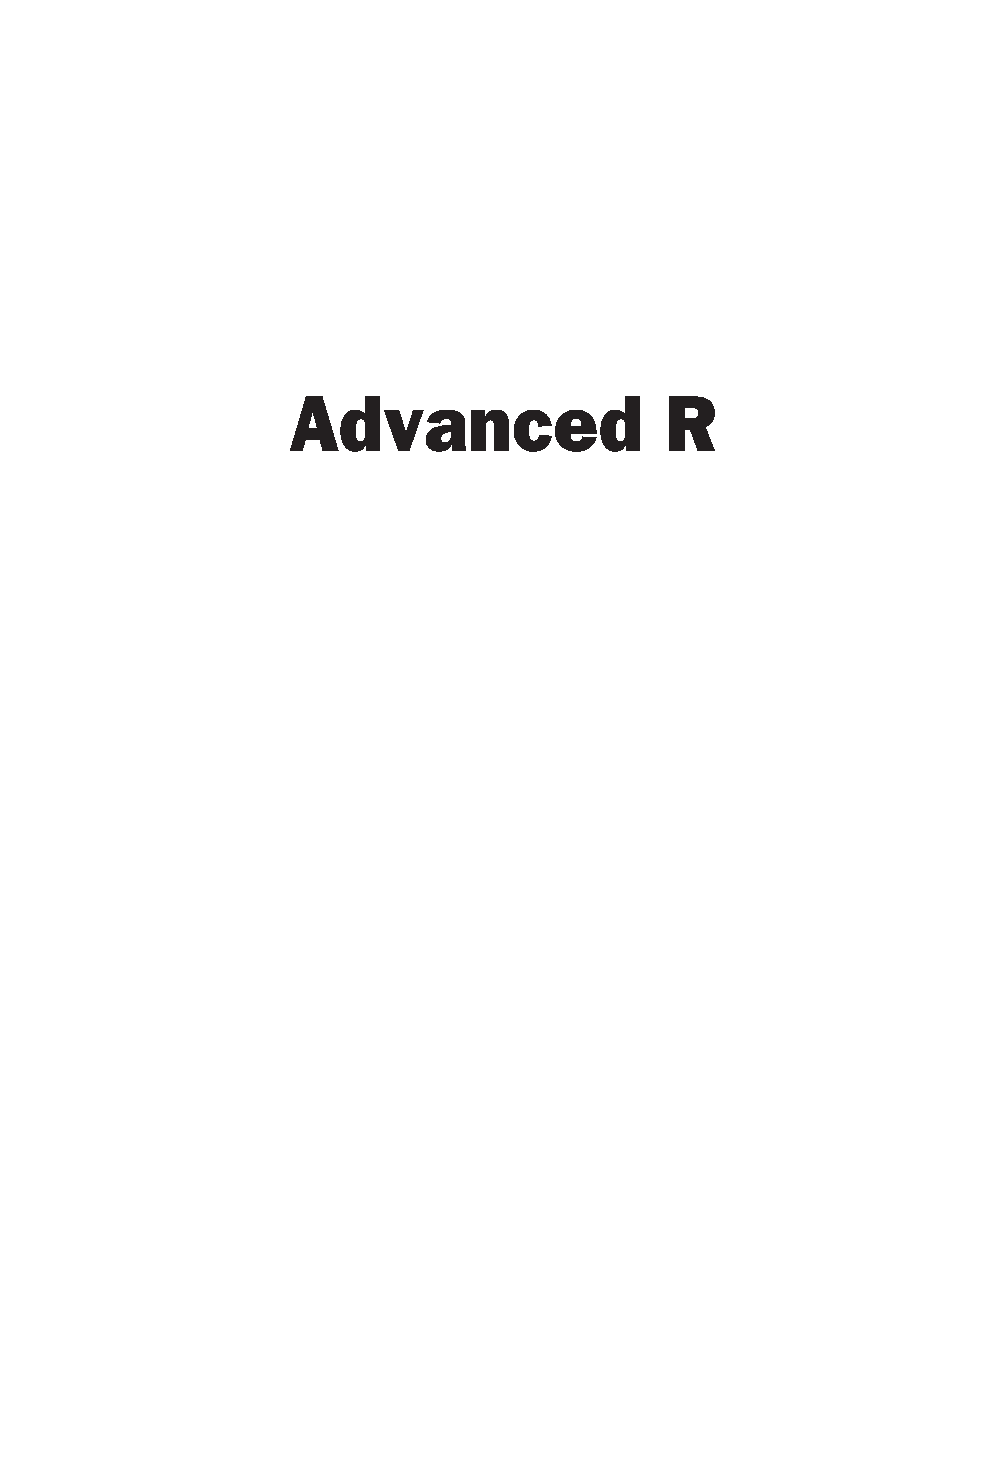
\includegraphics{K20319_FM1}}

\clearpage\vspace*{-69pt}
\centerline{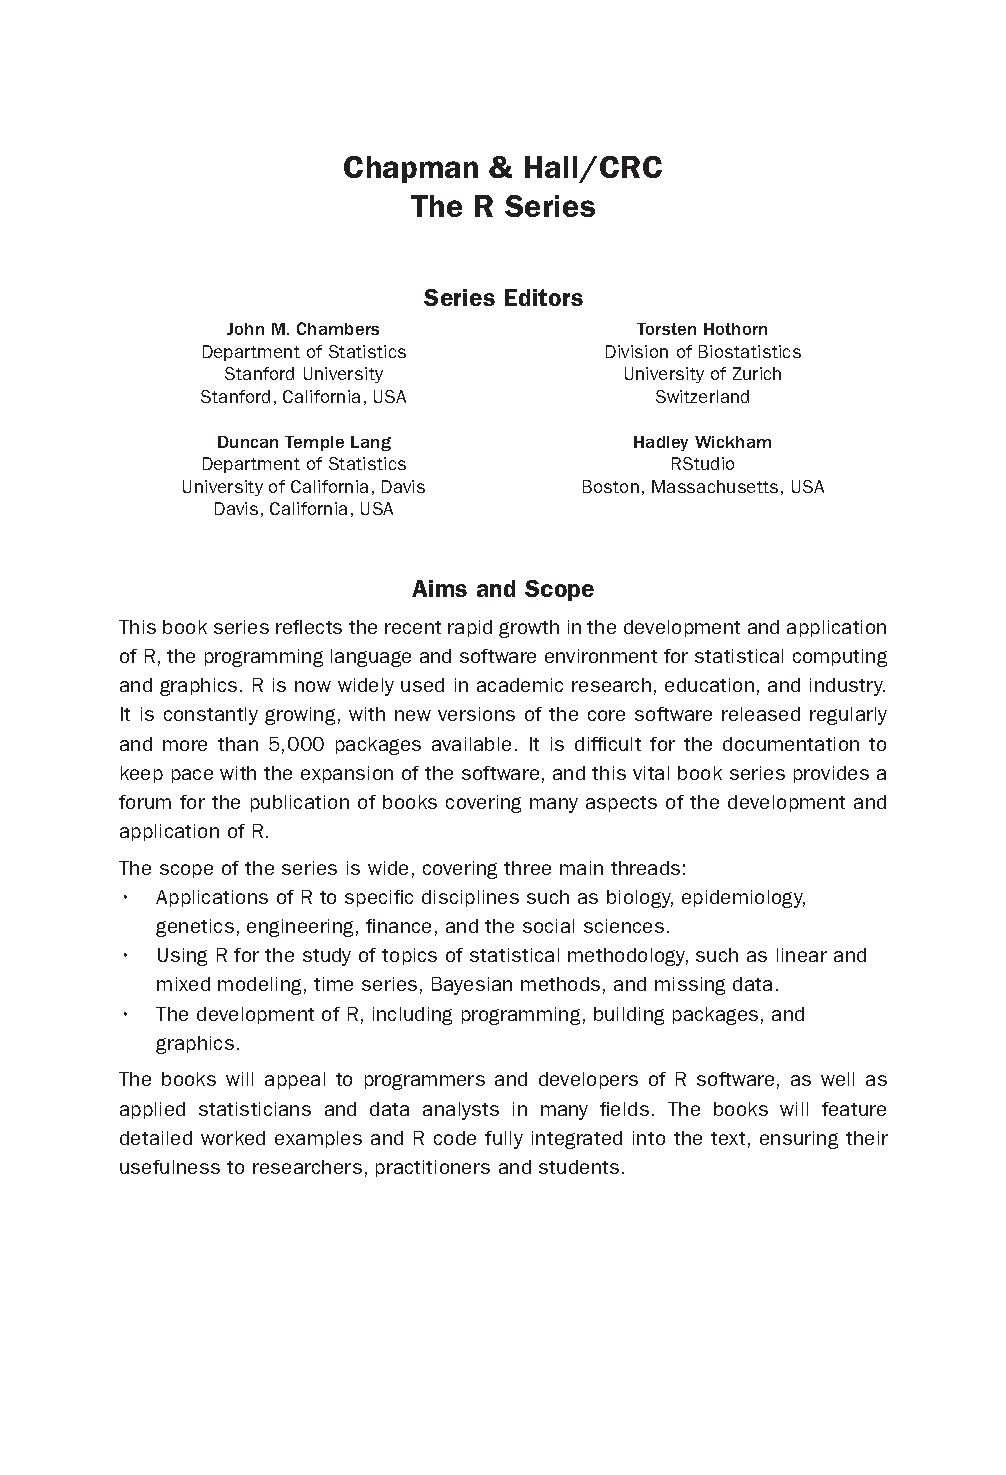
\includegraphics{K20319_FM2}}

\clearpage\vspace*{-69pt}
\centerline{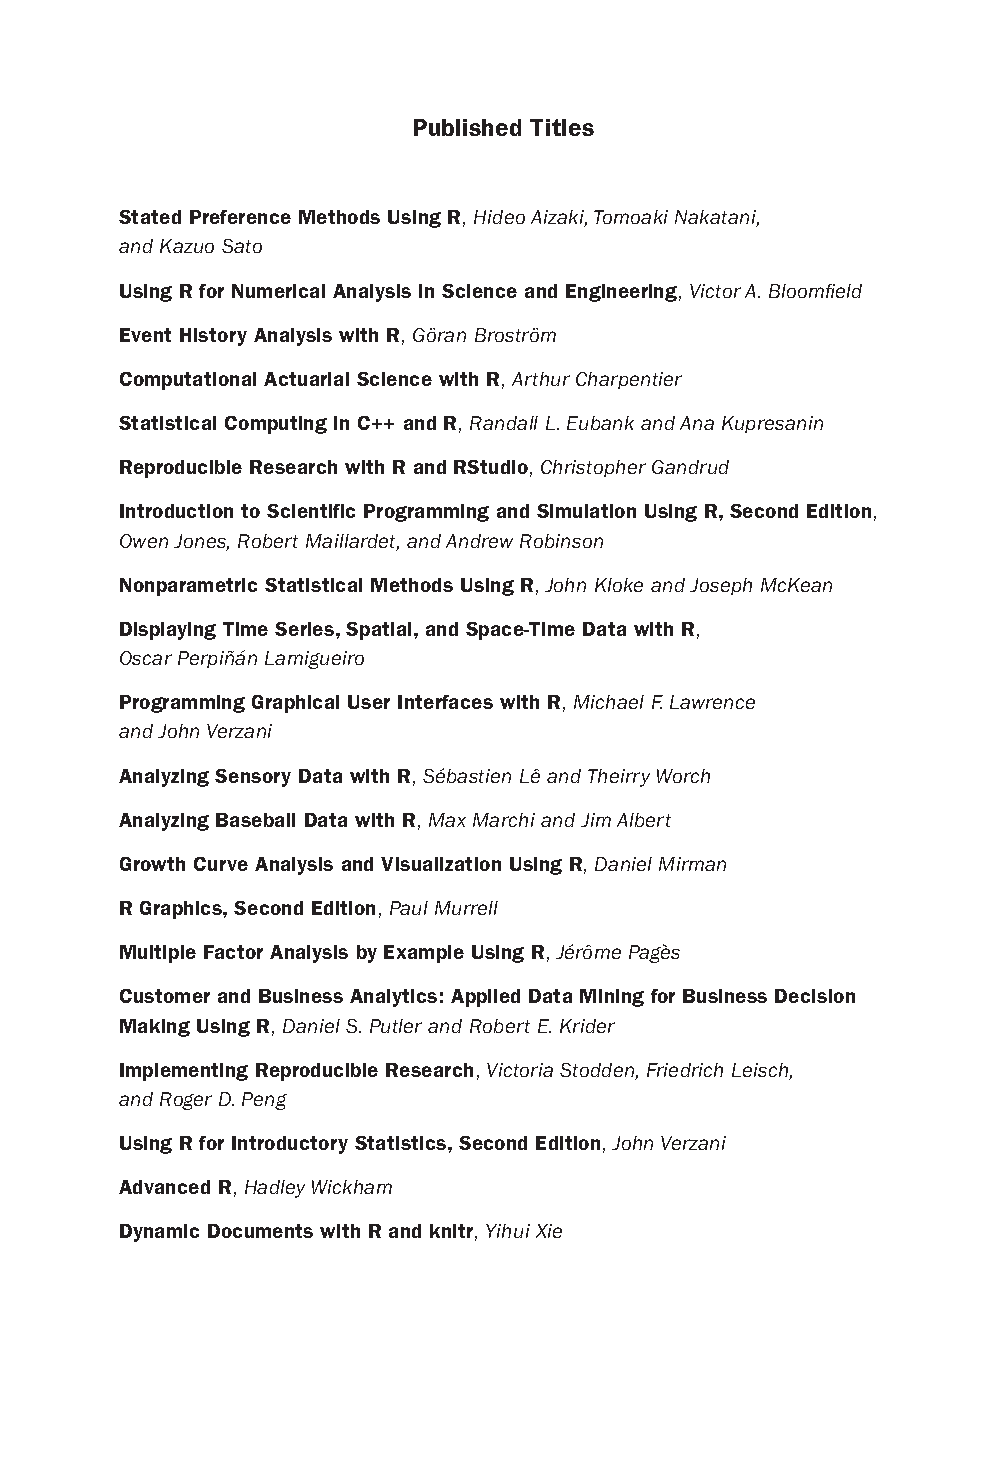
\includegraphics{K20319_FM3}}

\clearpage\vspace*{-69pt}
\centerline{
\includegraphics{K20319_FM4}}

\clearpage\vspace*{-69pt}
\centerline{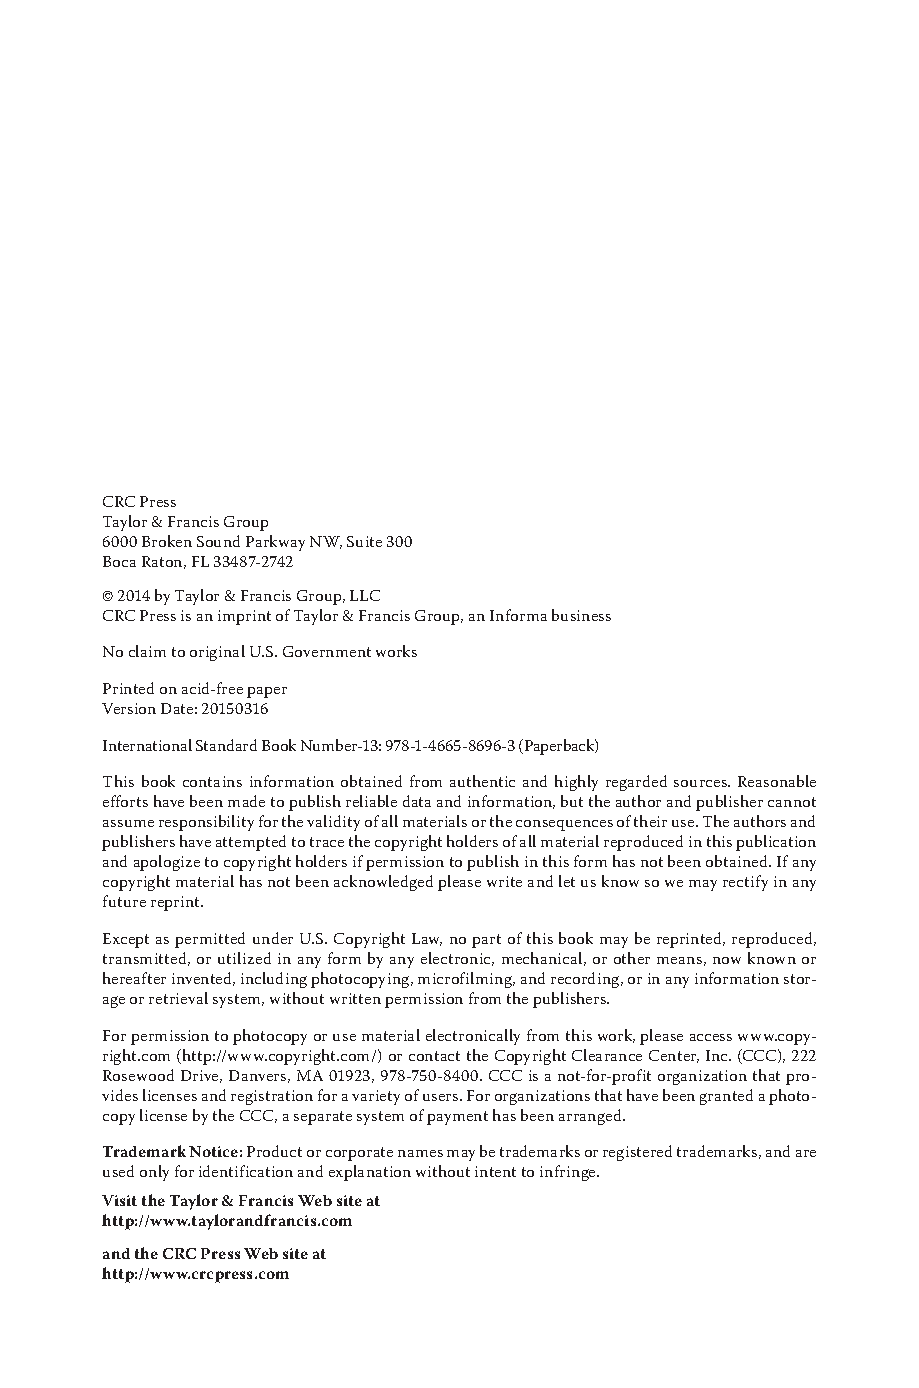
\includegraphics{K20319_Paperback_Discl}}



\frontmatter\pagestyle{headings}
%\maketitle

\setcounter{page}{7}
\cleardoublepage
\vspace*{\stretch{1}}
\hfill
\begin{minipage}[t]{0.66\textwidth}
\raggedleft
\thispagestyle{empty}
\textit{To Jeff, who makes me happy, and who made sure I had a life outside this book.}
\end{minipage}
\vspace*{\stretch{3}}
\clearpage
% \listoffigures
% \listoftables
\tableofcontents

\mainmatter


\chapter{Introduction}
\label{introduction}

With more than 10 years experience programming in R, I've had the luxury
of being able to spend a lot time trying to figure out and understand
how the language works. This book is my attempt to pass on what I've
learned so you can quickly become an effective R programmer. Reading it
will help you avoid the mistakes I've made and dead ends I've gone down,
and will teach you useful tools, techniques and idioms that can help you
to attack many types of problems. In the process, I hope to show that,
despite its frustrating quirks, R is, at its heart, an elegant and
beautiful language, well tailored for data analysis and statistics.

If you are new to R, you might wonder what makes learning such a quirky
language worthwhile. To me, some of the best features are:

\begin{itemize}
\item
  Free, open source and available on every major platform. As a result,
  if you do your analysis in R, anyone can easily replicate it.
\item
  A massive set of packages for statistical modelling, machine learning,
  visualisation, and the importing and manipulation of data. Whatever
  model or visualisation you're trying to do, chances are that someone
  has already tried to do it. At a minimum, you can learn from their
  efforts.
\item
  Cutting edge tools. Researchers in statistics and machine learning
  will often publish an R package to accompany their articles. This
  means immediate access to the very latest statistical techniques and
  implementations.
\item
  Deep-seated support in the language for data analysis. This includes
  features likes missing values, data frames, and subsetting.
\item
  A fantastic community. It is easy to get help from experts on the
  \href{https://stat.ethz.ch/mailman/listinfo/r-help}{R-help mailing
  list},
  \href{http://stackoverflow.com/questions/tagged/r}{stackoverflow}, or
  subject specific mailing lists like
  \href{https://stat.ethz.ch/mailman/listinfo/r-sig-mixed-models}{R-SIG-mixed-models}
  or \href{https://groups.google.com/forum/\#!forum/ggplot2}{ggplot2}.
  You can also connect with other R learners via
  \href{https://twitter.com/search?q=\%23rstats}{twitter},
  \href{http://www.linkedin.com/groups/R-Project-Statistical-Computing-77616}{linkedin},
  and through many local
  \href{http://blog.revolutionanalytics.com/local-r-groups.html}{user
  groups}.
\item
  Powerful tools for communicating your results. R packages make it easy
  to produce html or pdf \href{http://yihui.name/knitr/}{reports}, or
  create \href{http://www.rstudio.com/shiny/}{interactive websites}.
\item
  A strong foundation in functional programming. The ideas of functional
  programming are well suited to solving many of the challenges of data
  analysis. This helps R provide a powerful and flexible toolkit which
  allows you to write concise yet descriptive code.
\item
  An \href{http://www.rstudio.com/ide/}{IDE} tailored to the needs of
  interactive data analysis and statistical programming.
\item
  Powerful metaprogramming facilities. R is not just a programming
  language, it is also an environment for interactive data analysis. Its
  metaprogramming capabilities allow you to write magically succinct and
  concise functions and provides an excellent environment for designing
  domain specific languages.
\item
  Designed to connect to high-performance programming languages like C,
  Fortran and C++.
\end{itemize}

Of course, R is not perfect. R's biggest challenge is that most R users
are not programmers. This means that:

\begin{itemize}
\item
  Much of the R code you'll see in the wild is usually written in haste
  to solve a pressing problem. As a result, code is not very elegant,
  fast or easy to understand. Also, users do not revise code to address
  those shortcomings.
\item
  Compared to other programming languages, the R community tends to be
  more focussed on results instead of processes. Knowledge of software
  engineering best practices is patchy: for instance, not enough R
  programmers use source code control or automated testing.
\item
  Metaprogramming is a double-edged sword. Too many R functions use
  tricks to reduce the amount of typing at the cost of making code that
  is hard to understand and that can fail in unexpected ways.
\item
  Inconsistency is rife across contributed packages, even within base R.
  The R APIs have evolved over 20 years. You are confronted with this
  fact every time you use R. Having to memorise many special cases makes
  learning R tough.
\item
  R is not a particularly fast programming language. Poorly written R
  code can be terribly slow. R is also a profligate user of memory.
  Tools for parallel processing are not mature.
\end{itemize}

Personally, I think these challenges create a great opportunity for
experienced programmers to have a profound positive impact on R and the
R community. R users do care about writing high quality code,
particularly for reproducible research, but they don't yet have the
skills to do so. I hope this book will not only encourage programmers
from other languages to contribute to R but to also help more R users to
become R programmers.

\section{Who should read this book}\label{who-should-read-this-book}

This book is aimed at two complementary audiences:

\begin{itemize}
\item
  Intermediate R programmers who want to dive deeper into R and learn
  new strategies for solving diverse problems
\item
  Programmers from other languages who are learning R and want to
  understand why R works the way it does.
\end{itemize}

To get the most out of this book, you'll need to have written a decent
amount of code in either R or other programming languages. Although you
might not know all the details, you should be familiar with how
functions work in R and although you may currently struggle to use them
effectively, you should be somewhat familiar with the apply family of
functions (like \texttt{apply()} and \texttt{lapply()}).

\section{What you will get out of this
book}\label{what-you-will-get-out-of-this-book}

This book describes the skills I think an advanced R programmer should
have: the ability to produce reusable code that can be used in a wide
variety of circumstances.

After reading this book, you will:

\begin{itemize}
\item
  Be familiar with the fundamentals of R. You will understand complex
  data types and the best ways to perform operations on them.You will
  have a deep understanding of how functions work, and be able to
  recognise and use the four object systems in R.
\item
  Understand what functional programming means, and why it is useful
  tool for data analysis. You'll be able to quickly learn how to use
  existing tools, and have the knowledge to create your own functional
  tools when needed.
\item
  Appreciate the double-edged sword of metaprogramming. You'll be able
  to create functions that use non-standard evaluation in a principled
  way, saving typing and creating elegant code to expressing important
  operations. You'll also understand the dangers of metaprogramming and
  why you should be careful about its use.
\item
  Have a good intuition for which operations in R are slow or use a lot
  of memory. You'll know how to use profiling to pinpoint performance
  bottlenecks, and you'll know enough C++ to convert slow R functions to
  fast C++ equivalents.
\item
  Be comfortable reading and understanding the majority of R code.
  You'll recognise common idioms (even if you wouldn't use them
  yourself) and be able to critique others' code.
\end{itemize}

\section{Meta-techniques}\label{meta-techniques}

There are two meta-techniques that are tremendously helpful for
improving your skills as an R programmer: reading source code and
adopting a scientific mindset.

Reading source code is important because it'll help you write better
code. A great place to start developing this skill would be looking at
source code of the functions and packages you use most. Through exposure
to new ways of doing things, you'll find things that are worth emulating
in your own code and you'll develop a sense of taste for what makes good
R code. This exposure is also valuable because of the things you may not
like either because their virtues are not be obvious or because they
might violate your sensibilities. Such things are nonetheless valuable
because they expose you to the idioms and styles used by other
programmers. This ability to read any code becomes particularly
important when you start using the more esoteric parts of R. Since the
documentation there will often be lacking, the only way to figure out
how a function works will depend on your ability to understand and
experiment with the source code.

A scientific mindset is extremely helpful when learning R. If you don't
understand how something works, develop a hypothesis, design some
experiments, run them and record the results. This exercise is extremely
useful since if you can't figure something out and need to get help, you
can easily show others what you tried. Also, when you learn the right
answer, you'll be mentally prepared to update your world view. I often
find that when I clearly describe a problem to someone else (the art of
creating a
\href{http://stackoverflow.com/questions/5963269}{reproducible
example}), I figure out the solution myself.

\section{Recommended reading}\label{recommended-reading}

R is still a relatively young language, and the resources to help you
understand it are still maturing. In my personal journey to understand
R, I've found it particularly helpful to refer to resources from other
programming languages. R has aspects of both functional and
object-oriented (OO) programming languages. Learning how these concepts
are expressed in R will help you leverage your existing knowledge of
other programming languages, and will help you identify areas where you
can improve.

To understand why R's object systems work the way they do, I found
\href{http://mitpress.mit.edu/sicp/full-text/book/book.html}{The
Structure and Interpretation of Computer Programs} (SICP) by Harold
Abelson and Gerald Jay Sussman, particularly helpful. It's a concise but
deep book. After reading it, I felt for the first time that I could
actually design my own object-oriented system. The book was my first
introduction to the generic function style of OO common in R. It helped
me understand its strengths and weaknesses. SICP also talks a lot about
functional programming, and how to create simple functions which become
powerful when combined.

To understand the tradeoffs that R has made compared to other
programming languages, I found
\href{http://amzn.com/0262220695?tag=devtools-20}{Concepts, Techniques
and Models of Computer Programming} by Peter van Roy and Sef Haridi
extremely helpful. It helped me understand that R's copy-on-modify
semantics make it substantially easier to reason about code, and that
while its current implementation is not particularly efficient, it is a
solvable problem.

If you want to learn to be a better programmer, there's no place better
to turn than \href{http://amzn.com/020161622X?tag=devtools-20}{The
Pragmatic Programmer} by Andrew Hunt and David Thomas. This book is
language agnostic, and provides great advice for how to be a better
programmer.

\section{Getting help}\label{getting-help}

Currently, there are two main venues to get help when you're stuck and
can't figure out what's causing the problem:
\href{http://stackoverflow.com}{stackoverflow} and the R-help mailing
list. You can get fantastic help in both venues, but they do have their
own cultures and expectations. It's usually a good idea to spend a
little time lurking, learning about community expectations, before you
put up your first post.

Some good general advice:

\begin{itemize}
\item
  Make sure you have the latest version of R and of the package (or
  packages) you are having problems with. It may be that your problem is
  the result of a recently fixed bug.
\item
  Spend some time creating a
  \href{http://stackoverflow.com/questions/5963269}{reproducible
  example}. This is often a useful process in its own right, because in
  the course of making the problem reproducible you often figure out
  what's causing the problem.
\item
  Look for related problems before posting. If someone has already asked
  your question and it has been answered, it's much faster for everyone
  if you use the existing answer.
\end{itemize}

\section{Acknowledgements}\label{intro-ack}

I would like to thank the tireless contributors to R-help and, more
recently,
\href{http://stackoverflow.com/questions/tagged/r}{stackoverflow}. There
are too many to name individually, but I'd particularly like to thank
Luke Tierney, John Chambers, Dirk Eddelbuettel, JJ Allaire and Brian
Ripley for generously giving their time and correcting my countless
misunderstandings.

This book was \href{https://github.com/hadley/adv-r/}{written in the
open}, and chapters were advertised on
\href{https://twitter.com/hadleywickham}{twitter} when complete. It is
truly a community effort: many people read drafts, fixed typos,
suggested improvements and contributed content. Without those
contributors, the book wouldn't be nearly as good as it is, and I'm
deeply grateful for their help. Special thanks go to Peter Li, who read
the book from cover-to-cover and provided many fixes. Other outstanding
contributors were Aaron Schumacher, @crtahlin, Lingbing Feng,
@juancentro and @johnbaums.

Thanks go to all contributers in alphabetical order: Aaron Schumacher,
Aaron Wolen, @aaronwolen, @absolutelyNoWarranty, Adam Hunt, @agrabovsky,
@ajdm, @alexbbrown, @allegretto, @AmeliaMN, @andrewla, Andy Teucher,
Anton Antonov, @aranlunzer, @arilamstein, @avilella, @baptiste,
@blindjesse, @blmoore, @bnjmn, Brandon Hurr, @BrianDiggs, @Bryce, C.
Jason Liang, @Carson, @cdrv, Ching Boon, @chiphogg, Christopher Brown,
@christophergandrud, Clay Ford, @cornelius1729, @cplouffe, Craig Citro,
@crossfitAL, @crowding, Crt Ahlin, @crtahlin, @cscheid, @csgillespie,
@cusanovich, @cwarden, @cwickham, Daniel Lee, @darrkj, @Dasonk, David
Hajage, David LeBauer, @dchudz, dennis feehan, @dfeehan, Dirk
Eddelbuettel, @dkahle, @dlebauer, @dlschweizer, @dmontaner,
@dougmitarotonda, @dpatschke, @duncandonutz, @EdFineOKL, @EDiLD,
@eipi10, @elegrand, @EmilRehnberg, Eric C. Anderson, @etb, @fabian-s,
Facundo Muñoz, @flammy0530, @fpepin, Frank Farach, @fyears, Garrett
Grolemund, @garrettgman, @gavinsimpson, @gggtest, Gökçen Eraslan,
@gregorp, @gsee, @gsk3, @gthb, @hassaad85, @i, Iain Dillingham,
@ijlyttle, Ilan Man, @imanuelcostigan, @initdch, Jason Asher, Jason
Knight, @jasondavies, @jastingo, @jcborras, Jeff Allen, @jeharmse,
@jentjr, @JestonBlu, @JimInNashville, @jinlong25, JJ Allaire, Jochen Van
de Velde, Johann Hibschman, John Blischak, john verzani, @johnbaums,
@johnjosephhorton, @juancentro, @kdauria, @kenahoo, @kent37, Kevin
Markham, Kevin Ushey, @kforner, Kirill Müller, Kun Ren, Laurent Gatto,
@Lawrence-Liu, @ldfmrails, @lgatto, @liangcj, Lingbing Feng, @lynaghk,
Maarten Kruijver, Mamoun Benghezal, @mannyishere, Matt Pettis,
@mattbaggott, Matthew Grogan, @mattmalin, Michael Kane, @michaelbach,
@mjsduncan, @Mullefa, @myqlarson, Nacho Caballero, Nick Carchedi,
@nstjhp, @ogennadi, Oliver Keyes, Parker Abercrombie, @patperu, @pdb61,
@pengyu, Peter F Schulam, Peter Lindbrook, Peter Meilstrup,
@philchalmers, @picasa, @piccolbo, @pierreroudier, @pooryorick, R. Mark
Sharp, Ramnath Vaidyanathan, @ramnathv, @Rappster, Ricardo Pietrobon,
Richard Cotton, @richardreeve, @rmflight, @rmsharp, Robert M Flight,
@RobertZK, @robiRagan, Romain François, @rubenfcasal, @sailingwave,
@sbgraves237, Scott Ritchie, @scottko, @scottl, Sean Anderson, Sean
Carmody, Sean Wilkinson, @sebastian-c, @shabbychef, Shannon Rush, Simon
O'Hanlon, Simon Potter, @ste-fan, Stefan Widgren, @stephens999, Steven
Pav, @strongh, @stuttungur, @surmann, @swnydick, @taekyunk, Tal Galili,
@talgalili, @tdenes, @Thomas, @thomasherbig, @thomaszumbrunn, Tim Cole,
tj mahr, @tjmahr, Tom Buckley, Tom Crockett, @ttriche, @twjacobs,
@tyhenkaline, @tylerritchie, @ulrichatz, @varun729, @victorkryukov,
@vijaybarve, @vzemlys, @wchi144, @wibeasley, @WilCrofter, William Doane,
Winston Chang, @wmc3, @wordnerd, Yoni Ben-Meshulam, @zackham,
@zerokarmaleft, Zhongpeng Lin.

\section{Conventions}\label{conventions}

Throughout this book I use \texttt{f()} to refer to functions,
\texttt{g} to return to function parameters, and \texttt{h/} to paths.
Larger code blocks intermingle input and output. Output is placed in
comments so that you can copy and paste from electronic versions. Output
comments look like \texttt{\#\textgreater{}} to distinguish them regular
comments.

\section{Colophon}\label{colophon}

This book was written in \href{http://rmarkdown.rstudio.com/}{Rmarkdown}
inside \href{http://www.rstudio.com/ide/}{Rstudio}.
\href{http://yihui.name/knitr/}{knitr} and
\href{http://johnmacfarlane.net/pandoc/}{pandoc} converted the raw
Rmarkdown to html and pdf. The \href{http://adv-r.had.co.nz}{website}
was made with \href{http://jekyllrb.com/}{jekyll}, styled with
\href{http://getbootstrap.com/}{bootstrap}, and automatically published
to amazon's \href{http://aws.amazon.com/s3/}{S3} with
\href{https://github.com/laurilehmijoki/s3_website}{s3\_website} by
\href{https://travis-ci.org/}{travis-ci}. The complete source is
available from \href{https://github.com/hadley/adv-r}{github}.

Code is set in
\href{http://levien.com/type/myfonts/inconsolata.html}{inconsolata}.


\part{Foundations}
\chapter{Data structures}\label{data-structures}

This chapter summarises the most important data structures in base R.
You've probably used many (if not all) of them before, but you may not
have thought deeply about how they are interrelated. In this brief
overview, I won't discuss individual types in depth. Instead, I'll show
you how they fit together as a whole. If you need more details, you can
find them in R's documentation.

R's base data structures can be organised by their dimensionality (1d,
2d, or nd) and whether they're homogeneous (all contents must be of the
same type) or heterogeneous (the contents can be of different types).
This gives rise to the five data types most often used in data analysis:

\begin{longtable}[c]{@{}lll@{}}
\toprule\addlinespace
& Homogeneous & Heterogeneous
\\\addlinespace
\midrule\endhead
1d & Atomic vector & List
\\\addlinespace
2d & Matrix & Data frame
\\\addlinespace
nd & Array &
\\\addlinespace
\bottomrule
\end{longtable}

Almost all other objects are built upon these foundations. In
\hyperref[oo-field-guide]{the OO field guide} you'll see how more
complicated objects are built of these simple pieces. Note that R has
0-dimensional, or scalar types. Individual numbers or strings, which you
might think would be scalars, are actually vectors of length one.

Given an object, the best way to understand what data structures it's
composed of is to use \texttt{str()}. \texttt{str()} is short for
structure and it gives a compact, human readable description of any R
data structure.

\paragraph{Quiz}\label{quiz}

Take this short quiz to determine if you need to read this chapter. If
the answers quickly come to mind, you can comfortably skip this chapter.
You can check your answers in
\hyperref[data-structure-answers]{answers}.

\begin{enumerate}
\def\labelenumi{\arabic{enumi}.}
\item
  What are the three properties of a vector, other than its contents?
\item
  What are the four common types of atomic vectors? What are the two
  rare types?
\item
  What are attributes? How do you get them and set them?
\item
  How is a list different from an atomic vector? How is a matrix
  different from a data frame?
\item
  Can you have a list that is a matrix? Can a data frame have a column
  that is a matrix?
\end{enumerate}

\paragraph{Outline}\label{outline}

\begin{itemize}
\item
  \hyperref[vectors]{Vectors} introduces you to atomic vectors and
  lists, R's 1d data structures.
\item
  \hyperref[attributes]{Attributes} takes a small detour to discuss
  attributes, R's flexible metadata specification. Here you'll learn
  about factors, an important data structure created by setting
  attributes of an atomic vector.
\item
  \hyperref[matrices-and-arrays]{Matrices and arrays} introdues matrices
  and arrays, data structures for storing 2d and higher dimensional
  data.
\item
  \hyperref[data-frames]{Data frames} teaches you about the data frame,
  the most important data structure for storing data in R. Data frames
  combine the behaviour of lists and matrices to make a structure
  ideally suited for the needs of statistical data.
\end{itemize}

\hyperdef{}{vectors}{\section{Vectors}\label{vectors}}

The basic data structure in R is the vector. Vectors comes in two
flavours: atomic vectors and lists. They have three common properties:

\begin{itemize}
\itemsep1pt\parskip0pt\parsep0pt
\item
  Type, \texttt{typeof()}, what it is.
\item
  Length, \texttt{length()}, how many elements it contains.
\item
  Attributes, \texttt{attributes()}, additional arbitrary metadata.
\end{itemize}

They differ in the types of their elements: all elements of an atomic
vector must be the same type, whereas the elements of a list can have
different types.

NB: \texttt{is.vector()} does not test if an object is a vector. Instead
it returns \texttt{TRUE} only if the object is a vector with no
attributes apart from names. Use
\texttt{is.atomic(x) \textbar{}\textbar{} is.list(x)} to test if an
object is actually a vector.

\subsection{Atomic vectors}\label{atomic-vectors}

There are four common types of atomic vector that I'll discuss in
detail: logical, integer, double (often called numeric), and character.
There are two rare types that I will not discuss further: complex and
raw.

Atomic vectors are usually created with \texttt{c()}, short for combine:

\begin{Shaded}
\begin{Highlighting}[]
\NormalTok{dbl_var <-}\StringTok{ }\KeywordTok{c}\NormalTok{(}\DecValTok{1}\NormalTok{, }\FloatTok{2.5}\NormalTok{, }\FloatTok{4.5}\NormalTok{)}
\CommentTok{# With the L suffix, you get an integer rather than a double}
\NormalTok{int_var <-}\StringTok{ }\KeywordTok{c}\NormalTok{(1L, 6L, 10L)}
\CommentTok{# Use TRUE and FALSE (or T and F) to create logical vectors}
\NormalTok{log_var <-}\StringTok{ }\KeywordTok{c}\NormalTok{(}\OtherTok{TRUE}\NormalTok{, }\OtherTok{FALSE}\NormalTok{, T, F)}
\NormalTok{chr_var <-}\StringTok{ }\KeywordTok{c}\NormalTok{(}\StringTok{"these are"}\NormalTok{, }\StringTok{"some strings"}\NormalTok{)}
\end{Highlighting}
\end{Shaded}

Atomic vectors are always flat, even if you nest \texttt{c()}'s:

\begin{Shaded}
\begin{Highlighting}[]
\KeywordTok{c}\NormalTok{(}\DecValTok{1}\NormalTok{, }\KeywordTok{c}\NormalTok{(}\DecValTok{2}\NormalTok{, }\KeywordTok{c}\NormalTok{(}\DecValTok{3}\NormalTok{, }\DecValTok{4}\NormalTok{)))}
\CommentTok{#> [1] 1 2 3 4}
\CommentTok{# the same as}
\KeywordTok{c}\NormalTok{(}\DecValTok{1}\NormalTok{, }\DecValTok{2}\NormalTok{, }\DecValTok{3}\NormalTok{, }\DecValTok{4}\NormalTok{)}
\CommentTok{#> [1] 1 2 3 4}
\end{Highlighting}
\end{Shaded}

Missing values are specified with \texttt{NA}, which is a logical vector
of length 1. \texttt{NA} will always be coerced to the correct type if
used inside \texttt{c()}, or you can create NA's of a specific types
with \texttt{NA\_real\_} (a double vector), \texttt{NA\_integer\_} and
\texttt{NA\_character\_}.

\subsubsection{Types and tests}\label{types-and-tests}

Given a vector, you can determine its type with \texttt{typeof()}, or
check if it's a specific type with an ``is'' function:
\texttt{is.character()}, \texttt{is.double()}, \texttt{is.integer()},
\texttt{is.logical()}, or, more generally, \texttt{is.atomic()}.

\begin{Shaded}
\begin{Highlighting}[]
\NormalTok{int_var <-}\StringTok{ }\KeywordTok{c}\NormalTok{(1L, 6L, 10L)}
\KeywordTok{typeof}\NormalTok{(int_var)}
\CommentTok{#> [1] "integer"}
\KeywordTok{is.integer}\NormalTok{(int_var)}
\CommentTok{#> [1] TRUE}
\KeywordTok{is.atomic}\NormalTok{(int_var)}
\CommentTok{#> [1] TRUE}

\NormalTok{dbl_var <-}\StringTok{ }\KeywordTok{c}\NormalTok{(}\DecValTok{1}\NormalTok{, }\FloatTok{2.5}\NormalTok{, }\FloatTok{4.5}\NormalTok{)}
\KeywordTok{typeof}\NormalTok{(dbl_var)}
\CommentTok{#> [1] "double"}
\KeywordTok{is.double}\NormalTok{(dbl_var)}
\CommentTok{#> [1] TRUE}
\KeywordTok{is.atomic}\NormalTok{(dbl_var)}
\CommentTok{#> [1] TRUE}
\end{Highlighting}
\end{Shaded}

NB: \texttt{is.numeric()} is a general test for the ``numberliness'' of
a vector and returns \texttt{TRUE} for both integer and double vectors.
It is not a specific test for double vectors, which are often called
numeric.

\begin{Shaded}
\begin{Highlighting}[]
\KeywordTok{is.numeric}\NormalTok{(int_var)}
\CommentTok{#> [1] TRUE}
\KeywordTok{is.numeric}\NormalTok{(dbl_var)}
\CommentTok{#> [1] TRUE}
\end{Highlighting}
\end{Shaded}

\subsubsection{Coercion}\label{coercion}

All elements of an atomic vector must be the same type, so when you
attempt to combine different types they will be \textbf{coerced} to the
most flexible type. Types from least to most flexible are: logical,
integer, double and character.

For example, combining a character and an integer yields a character:

\begin{Shaded}
\begin{Highlighting}[]
\KeywordTok{str}\NormalTok{(}\KeywordTok{c}\NormalTok{(}\StringTok{"a"}\NormalTok{, }\DecValTok{1}\NormalTok{))}
\CommentTok{#>  chr [1:2] "a" "1"}
\end{Highlighting}
\end{Shaded}

When a logical vector is coerced to an integer or double, \texttt{TRUE}
becomes 1 and \texttt{FALSE} becomes 0. This is very useful in
conjunction with \texttt{sum()} and \texttt{mean()}

\begin{Shaded}
\begin{Highlighting}[]
\NormalTok{x <-}\StringTok{ }\KeywordTok{c}\NormalTok{(}\OtherTok{FALSE}\NormalTok{, }\OtherTok{FALSE}\NormalTok{, }\OtherTok{TRUE}\NormalTok{)}
\KeywordTok{as.numeric}\NormalTok{(x)}
\CommentTok{#> [1] 0 0 1}
\CommentTok{# Total number of TRUEs}
\KeywordTok{sum}\NormalTok{(x)}
\CommentTok{#> [1] 1}
\CommentTok{# Proportion of TRUEs}
\KeywordTok{mean}\NormalTok{(x)}
\CommentTok{#> [1] 0.3333}
\end{Highlighting}
\end{Shaded}

Coercion often happens automatically. Most mathematical functions
(\texttt{+}, \texttt{log}, \texttt{abs}, etc.) will coerce to a double
or integer, and most logical operations (\texttt{\&},
\texttt{\textbar{}}, \texttt{any}, etc) will coerce to a logical. You
will usually get a warning message if the coercion might lose
information. If confusion is likely, explicitly coerce with
\texttt{as.character()}, \texttt{as.double()}, \texttt{as.integer()}, or
\texttt{as.logical()}.

\subsection{Lists}\label{lists}

Lists are different from atomic vectors because their elements can be of
any type, including lists. You construct lists by using \texttt{list()}
instead of \texttt{c()}:

\begin{Shaded}
\begin{Highlighting}[]
\NormalTok{x <-}\StringTok{ }\KeywordTok{list}\NormalTok{(}\DecValTok{1}\NormalTok{:}\DecValTok{3}\NormalTok{, }\StringTok{"a"}\NormalTok{, }\KeywordTok{c}\NormalTok{(}\OtherTok{TRUE}\NormalTok{, }\OtherTok{FALSE}\NormalTok{, }\OtherTok{TRUE}\NormalTok{), }\KeywordTok{c}\NormalTok{(}\FloatTok{2.3}\NormalTok{, }\FloatTok{5.9}\NormalTok{))}
\KeywordTok{str}\NormalTok{(x)}
\CommentTok{#> List of 4}
\CommentTok{#>  $ : int [1:3] 1 2 3}
\CommentTok{#>  $ : chr "a"}
\CommentTok{#>  $ : logi [1:3] TRUE FALSE TRUE}
\CommentTok{#>  $ : num [1:2] 2.3 5.9}
\end{Highlighting}
\end{Shaded}

Lists are sometimes called \textbf{recursive} vectors, because a list
can contain other lists. This makes them fundamentally different from
atomic vectors.

\begin{Shaded}
\begin{Highlighting}[]
\NormalTok{x <-}\StringTok{ }\KeywordTok{list}\NormalTok{(}\KeywordTok{list}\NormalTok{(}\KeywordTok{list}\NormalTok{(}\KeywordTok{list}\NormalTok{())))}
\KeywordTok{str}\NormalTok{(x)}
\CommentTok{#> List of 1}
\CommentTok{#>  $ :List of 1}
\CommentTok{#>   ..$ :List of 1}
\CommentTok{#>   .. ..$ : list()}
\KeywordTok{is.recursive}\NormalTok{(x)}
\CommentTok{#> [1] TRUE}
\end{Highlighting}
\end{Shaded}

\texttt{c()} will combine several lists into one. If given a combination
of atomic vectors and lists, \texttt{c()} will coerce the vectors to
list before combining them. Compare the results of \texttt{list()} and
\texttt{c()}:

\begin{Shaded}
\begin{Highlighting}[]
\NormalTok{x <-}\StringTok{ }\KeywordTok{list}\NormalTok{(}\KeywordTok{list}\NormalTok{(}\DecValTok{1}\NormalTok{, }\DecValTok{2}\NormalTok{), }\KeywordTok{c}\NormalTok{(}\DecValTok{3}\NormalTok{, }\DecValTok{4}\NormalTok{))}
\NormalTok{y <-}\StringTok{ }\KeywordTok{c}\NormalTok{(}\KeywordTok{list}\NormalTok{(}\DecValTok{1}\NormalTok{, }\DecValTok{2}\NormalTok{), }\KeywordTok{c}\NormalTok{(}\DecValTok{3}\NormalTok{, }\DecValTok{4}\NormalTok{))}
\KeywordTok{str}\NormalTok{(x)}
\CommentTok{#> List of 2}
\CommentTok{#>  $ :List of 2}
\CommentTok{#>   ..$ : num 1}
\CommentTok{#>   ..$ : num 2}
\CommentTok{#>  $ : num [1:2] 3 4}
\KeywordTok{str}\NormalTok{(y)}
\CommentTok{#> List of 4}
\CommentTok{#>  $ : num 1}
\CommentTok{#>  $ : num 2}
\CommentTok{#>  $ : num 3}
\CommentTok{#>  $ : num 4}
\end{Highlighting}
\end{Shaded}

The \texttt{typeof()} a list is \texttt{list}, you can test for a list
with \texttt{is.list()} and coerce to a list with \texttt{as.list()}.
You can turn a list into an atomic vector with \texttt{unlist()}. If the
elements of a list have different types, \texttt{unlist()} uses the same
coercion rules as \texttt{c()},

Lists are used to build up many of the more complicated data structures
in R. For example, both data frames (described in
\hyperref[data-frames]{data frames}) and linear models objects (as
produced by \texttt{lm()}) are lists:

\begin{Shaded}
\begin{Highlighting}[]
\KeywordTok{is.list}\NormalTok{(mtcars)}
\CommentTok{#> [1] TRUE}

\NormalTok{mod <-}\StringTok{ }\KeywordTok{lm}\NormalTok{(mpg ~}\StringTok{ }\NormalTok{wt, }\DataTypeTok{data =} \NormalTok{mtcars)}
\KeywordTok{is.list}\NormalTok{(mod)}
\CommentTok{#> [1] TRUE}
\end{Highlighting}
\end{Shaded}

\subsection{Exercises}\label{exercises}

\begin{enumerate}
\def\labelenumi{\arabic{enumi}.}
\item
  What are the six types of atomic vector? How does a list differ from
  an atomic vector?
\item
  What makes \texttt{is.vector()} and \texttt{is.numeric()}
  fundamentally different to \texttt{is.list()} and
  \texttt{is.character()}?
\item
  Test your knowledge of vector coercion rules by predicting the output
  of the following uses of \texttt{c()}:

\begin{Shaded}
\begin{Highlighting}[]
\KeywordTok{c}\NormalTok{(}\DecValTok{1}\NormalTok{, }\OtherTok{FALSE}\NormalTok{)}
\KeywordTok{c}\NormalTok{(}\StringTok{"a"}\NormalTok{, }\DecValTok{1}\NormalTok{)}
\KeywordTok{c}\NormalTok{(}\KeywordTok{list}\NormalTok{(}\DecValTok{1}\NormalTok{), }\StringTok{"a"}\NormalTok{)}
\KeywordTok{c}\NormalTok{(}\OtherTok{TRUE}\NormalTok{, 1L)}
\end{Highlighting}
\end{Shaded}
\item
  Why do you need to use \texttt{unlist()} to convert a list to an
  atomic vector? Why doesn't \texttt{as.vector()} work?
\item
  Why is \texttt{1 == "1"} true? Why is \texttt{-1 \textless{} FALSE}
  true? Why is \texttt{"one" \textless{} 2} false?
\item
  Why is the default missing value, \texttt{NA}, a logical vector?
  What's special about logical vectors? (Hint: think about
  \texttt{c(FALSE, NA\_character\_)}.)
\end{enumerate}

\hyperdef{}{attributes}{\section{Attributes}\label{attributes}}

All objects can have arbitrary additional attributes, used to store
metadata about the object. Attributes can be thought of as a named list
(with unique names). Attributes can be accessed individually with
\texttt{attr()} or all at once (as a list) with \texttt{attributes()}.

\begin{Shaded}
\begin{Highlighting}[]
\NormalTok{y <-}\StringTok{ }\DecValTok{1}\NormalTok{:}\DecValTok{10}
\KeywordTok{attr}\NormalTok{(y, }\StringTok{"my_attribute"}\NormalTok{) <-}\StringTok{ "This is a vector"}
\KeywordTok{attr}\NormalTok{(y, }\StringTok{"my_attribute"}\NormalTok{)}
\CommentTok{#> [1] "This is a vector"}
\KeywordTok{str}\NormalTok{(}\KeywordTok{attributes}\NormalTok{(y))}
\CommentTok{#> List of 1}
\CommentTok{#>  $ my_attribute: chr "This is a vector"}
\end{Highlighting}
\end{Shaded}

The \texttt{structure()} function returns a new object with modified
attributes:

\begin{Shaded}
\begin{Highlighting}[]
\KeywordTok{structure}\NormalTok{(}\DecValTok{1}\NormalTok{:}\DecValTok{10}\NormalTok{, }\DataTypeTok{my_attribute =} \StringTok{"This is a vector"}\NormalTok{)}
\CommentTok{#>  [1]  1  2  3  4  5  6  7  8  9 10}
\CommentTok{#> attr(,"my_attribute")}
\CommentTok{#> [1] "This is a vector"}
\end{Highlighting}
\end{Shaded}

By default, most attributes are lost when modifying a vector:

\begin{Shaded}
\begin{Highlighting}[]
\KeywordTok{attributes}\NormalTok{(y[}\DecValTok{1}\NormalTok{])}
\CommentTok{#> NULL}
\KeywordTok{attributes}\NormalTok{(}\KeywordTok{sum}\NormalTok{(y))}
\CommentTok{#> NULL}
\end{Highlighting}
\end{Shaded}

The only attributes not lost are the three most important:

\begin{itemize}
\item
  Names, a character vector giving each element a names, descrbied in
  \hyperref[vector-names]{names}.
\item
  Dimensions, used to turn vectors into matrices and arrays, described
  in \hyperref[matrices-and-arrays]{matrices and arrays}.
\item
  Class, used to implement the S3 object system, described
  \hyperref[s3]{S3}.
\end{itemize}

Each of these attributes has a specific accessor function to get and
values. When working with these attributes, use \texttt{names(x)},
\texttt{class(x)} and \texttt{dim(x)}, not \texttt{attr(x, "names")},
\texttt{attr(x, "class")}, and \texttt{attr(x, "dim")}.

\hyperdef{}{vector-names}{\subsubsection{Names}\label{vector-names}}

You can name a vector in three ways:

\begin{itemize}
\item
  When creating it: \texttt{x \textless{}- c(a = 1, b = 2, c = 3)}.
\item
  By modifying an existing vector in place:
  \texttt{x \textless{}- 1:3; names(x) \textless{}- c("a", "b", "c")}.
\item
  By creating a modified copy of a vector:
  \texttt{x \textless{}- setNames(1:3, c("a", "b", "c"))}.
\end{itemize}

Names don't have to be unique. However, character subsetting,
\hyperref[lookup-tables]{subsetting}, is most important reason to use
names and it is most useful when the names are unique.

Not all elements of a vector need to have a name. If some names are
missing, \texttt{names()} will return an empty string for those
elements. If all names are missing, \texttt{names()} will return
\texttt{NULL}.

\begin{Shaded}
\begin{Highlighting}[]
\NormalTok{y <-}\StringTok{ }\KeywordTok{c}\NormalTok{(}\DataTypeTok{a =} \DecValTok{1}\NormalTok{, }\DecValTok{2}\NormalTok{, }\DecValTok{3}\NormalTok{)}
\KeywordTok{names}\NormalTok{(y)}
\CommentTok{#> [1] "a" ""  ""}

\NormalTok{z <-}\StringTok{ }\KeywordTok{c}\NormalTok{(}\DecValTok{1}\NormalTok{, }\DecValTok{2}\NormalTok{, }\DecValTok{3}\NormalTok{)}
\KeywordTok{names}\NormalTok{(z)}
\CommentTok{#> NULL}
\end{Highlighting}
\end{Shaded}

You can create a new vector without names using \texttt{unname(x)}, or
remove names in place with \texttt{names(x) \textless{}- NULL}.

\subsection{Factors}\label{factors}

One important application of attributes is the factor. A factor is a
vector that can contain only predefined values, and is used to store
categorical data. Factors are built on top of integer vectors using two
attributes: the \texttt{class()}, ``factor'', which makes them behave
differently to regular integer vectors, and the \texttt{levels()}, which
defines the set of allowed values.

\begin{Shaded}
\begin{Highlighting}[]
\NormalTok{x <-}\StringTok{ }\KeywordTok{factor}\NormalTok{(}\KeywordTok{c}\NormalTok{(}\StringTok{"a"}\NormalTok{, }\StringTok{"b"}\NormalTok{, }\StringTok{"b"}\NormalTok{, }\StringTok{"a"}\NormalTok{))}
\NormalTok{x}
\CommentTok{#> [1] a b b a}
\CommentTok{#> Levels: a b}
\KeywordTok{class}\NormalTok{(x)}
\CommentTok{#> [1] "factor"}
\KeywordTok{levels}\NormalTok{(x)}
\CommentTok{#> [1] "a" "b"}

\CommentTok{# You can't use values that are not in the levels}
\NormalTok{x[}\DecValTok{2}\NormalTok{] <-}\StringTok{ "c"}
\CommentTok{#> Warning: invalid factor level, NA generated}
\NormalTok{x}
\CommentTok{#> [1] a    <NA> b    a   }
\CommentTok{#> Levels: a b}

\CommentTok{# NB: you can't combine factors}
\KeywordTok{c}\NormalTok{(}\KeywordTok{factor}\NormalTok{(}\StringTok{"a"}\NormalTok{), }\KeywordTok{factor}\NormalTok{(}\StringTok{"b"}\NormalTok{))}
\CommentTok{#> [1] 1 1}
\end{Highlighting}
\end{Shaded}

Factors are useful when you know the possible values a variable may
take, even if you don't see all values in a given dataset. Using a
factor instead of a character vector makes it obvious when some groups
contain no observations:

\begin{Shaded}
\begin{Highlighting}[]
\NormalTok{sex_char <-}\StringTok{ }\KeywordTok{c}\NormalTok{(}\StringTok{"m"}\NormalTok{, }\StringTok{"m"}\NormalTok{, }\StringTok{"m"}\NormalTok{)}
\NormalTok{sex_factor <-}\StringTok{ }\KeywordTok{factor}\NormalTok{(sex_char, }\DataTypeTok{levels =} \KeywordTok{c}\NormalTok{(}\StringTok{"m"}\NormalTok{, }\StringTok{"f"}\NormalTok{))}

\KeywordTok{table}\NormalTok{(sex_char)}
\CommentTok{#> sex_char}
\CommentTok{#> m }
\CommentTok{#> 3}
\KeywordTok{table}\NormalTok{(sex_factor)}
\CommentTok{#> sex_factor}
\CommentTok{#> m f }
\CommentTok{#> 3 0}
\end{Highlighting}
\end{Shaded}

Sometimes when a data frame is read directly from a file, a column you'd
thought would produce a numeric vector instead produces a factor. This
is caused by a non-numeric value in the column, often a missing value
encoded in a special way like \texttt{.} or \texttt{-}. To remedy the
situation, coerce the vector from a factor to a character vector, and
then from a character to a double vector. (Be sure to check for missing
values after this process.) Of course, a much better plan is to discover
what caused the problem in the first place and fix that; using the
\texttt{na.strings} argument to \texttt{read.csv()} is often a good
place to start.

\begin{Shaded}
\begin{Highlighting}[]
\CommentTok{# Reading in "text" instead of from a file here:}
\NormalTok{z <-}\StringTok{ }\KeywordTok{read.csv}\NormalTok{(}\DataTypeTok{text=}\StringTok{"value}\CharTok{\textbackslash{}n}\StringTok{12}\CharTok{\textbackslash{}n}\StringTok{1}\CharTok{\textbackslash{}n}\StringTok{.}\CharTok{\textbackslash{}n}\StringTok{9"}\NormalTok{)}
\KeywordTok{typeof}\NormalTok{(z$value)}
\CommentTok{#> [1] "integer"}
\KeywordTok{as.double}\NormalTok{(z$value)}
\CommentTok{#> [1] 3 2 1 4}
\CommentTok{# Oops, that's not right: 3 2 1 4 are the levels of a factor, }
\CommentTok{# not the values we read in!}
\KeywordTok{class}\NormalTok{(z$value)}
\CommentTok{#> [1] "factor"}
\CommentTok{# We can fix it now:}
\KeywordTok{as.double}\NormalTok{(}\KeywordTok{as.character}\NormalTok{(z$value))}
\CommentTok{#> Warning: NAs introduced by coercion}
\CommentTok{#> [1] 12  1 NA  9}
\CommentTok{# Or change how we read it in:}
\NormalTok{z <-}\StringTok{ }\KeywordTok{read.csv}\NormalTok{(}\DataTypeTok{text=}\StringTok{"value}\CharTok{\textbackslash{}n}\StringTok{12}\CharTok{\textbackslash{}n}\StringTok{1}\CharTok{\textbackslash{}n}\StringTok{.}\CharTok{\textbackslash{}n}\StringTok{9"}\NormalTok{, }\DataTypeTok{na.strings=}\StringTok{"."}\NormalTok{)}
\KeywordTok{typeof}\NormalTok{(z$value)}
\CommentTok{#> [1] "integer"}
\KeywordTok{class}\NormalTok{(z$value)}
\CommentTok{#> [1] "integer"}
\NormalTok{z$value}
\CommentTok{#> [1] 12  1 NA  9}
\CommentTok{# Perfect! :)}
\end{Highlighting}
\end{Shaded}

Unfortunately, most data loading functions in R automatically convert
character vectors to factors. This is suboptimal, because there's no way
for those functions to know the set of all possible levels or their
optimal order. Instead, use the argument
\texttt{stringsAsFactors = FALSE} to suppress this behaviour, and then
manually convert character vectors to factors using your knowledge of
the data. A global option, \texttt{options(stringsAsFactors = FALSE)},
is available to control this behaviour, but I don't recommend using it.
Changing a global option may have unexpected consequences when combined
with other code (either from packages, or code that you're
\texttt{source()}ing), and global options make code harder to understand
because they increase the number of lines you need to read to understand
how a single line of code will behave.

While factors look (and often behave) like character vectors, they are
actually integers. Be careful when treating them like strings. Some
string methods (like \texttt{gsub()} and \texttt{grepl()}) will coerce
factors to strings, while others (like \texttt{nchar()}) will throw an
error, and still others (like \texttt{c()}) will use the underlying
integer values. For this reason, it's usually best to explicitly convert
factors to character vectors if you need string-like behaviour. In early
versions of R, there was a memory advantage to using factors instead of
character vectors, but this is no longer the case.

\subsection{Exercises}\label{exercises-1}

\begin{enumerate}
\def\labelenumi{\arabic{enumi}.}
\item
  An early draft used this code to illustrate \texttt{structure()}:

\begin{Shaded}
\begin{Highlighting}[]
\KeywordTok{structure}\NormalTok{(}\DecValTok{1}\NormalTok{:}\DecValTok{5}\NormalTok{, }\DataTypeTok{comment =} \StringTok{"my attribute"}\NormalTok{)}
\CommentTok{#> [1] 1 2 3 4 5}
\end{Highlighting}
\end{Shaded}

  But when you print that object you don't see the comment attribute.
  Why? Is the attribute missing, or is there something else special
  about it? (Hint: try using help)
\item
  What happens to a factor when you modify its levels?

\begin{Shaded}
\begin{Highlighting}[]
\NormalTok{f1 <-}\StringTok{ }\KeywordTok{factor}\NormalTok{(letters)}
\KeywordTok{levels}\NormalTok{(f1) <-}\StringTok{ }\KeywordTok{rev}\NormalTok{(}\KeywordTok{levels}\NormalTok{(f1))}
\end{Highlighting}
\end{Shaded}
\item
  What does this code do? How do \texttt{f2} and \texttt{f3} differ from
  \texttt{f1}?

\begin{Shaded}
\begin{Highlighting}[]
\NormalTok{f2 <-}\StringTok{ }\KeywordTok{rev}\NormalTok{(}\KeywordTok{factor}\NormalTok{(letters))}

\NormalTok{f3 <-}\StringTok{ }\KeywordTok{factor}\NormalTok{(letters, }\DataTypeTok{levels =} \KeywordTok{rev}\NormalTok{(letters))}
\end{Highlighting}
\end{Shaded}
\end{enumerate}

\hyperdef{}{matrices-and-arrays}{\section{Matrices and
arrays}\label{matrices-and-arrays}}

Adding a \texttt{dim()} attribute to an atomic vector allows it to
behave like a multi-dimensional \textbf{array}. A special case of the
array is the \textbf{matrix}, which has two dimensions. Matrices are
used commonly as part of the mathematical machinery of statistics.
Arrays are much rarer, but worth being aware of.

Matrices and arrays are created with \texttt{matrix()} and
\texttt{array()}, or by using the assignment form of \texttt{dim()}:

\begin{Shaded}
\begin{Highlighting}[]
\CommentTok{# Two scalar arguments to specify rows and columns}
\NormalTok{a <-}\StringTok{ }\KeywordTok{matrix}\NormalTok{(}\DecValTok{1}\NormalTok{:}\DecValTok{6}\NormalTok{, }\DataTypeTok{ncol =} \DecValTok{3}\NormalTok{, }\DataTypeTok{nrow =} \DecValTok{2}\NormalTok{)}
\CommentTok{# One vector argument to describe all dimensions}
\NormalTok{b <-}\StringTok{ }\KeywordTok{array}\NormalTok{(}\DecValTok{1}\NormalTok{:}\DecValTok{12}\NormalTok{, }\KeywordTok{c}\NormalTok{(}\DecValTok{2}\NormalTok{, }\DecValTok{3}\NormalTok{, }\DecValTok{2}\NormalTok{))}

\CommentTok{# You can also modify an object in place by setting dim()}
\NormalTok{c <-}\StringTok{ }\DecValTok{1}\NormalTok{:}\DecValTok{6}
\KeywordTok{dim}\NormalTok{(c) <-}\StringTok{ }\KeywordTok{c}\NormalTok{(}\DecValTok{3}\NormalTok{, }\DecValTok{2}\NormalTok{)}
\NormalTok{c}
\CommentTok{#>      [,1] [,2]}
\CommentTok{#> [1,]    1    4}
\CommentTok{#> [2,]    2    5}
\CommentTok{#> [3,]    3    6}
\KeywordTok{dim}\NormalTok{(c) <-}\StringTok{ }\KeywordTok{c}\NormalTok{(}\DecValTok{2}\NormalTok{, }\DecValTok{3}\NormalTok{)}
\NormalTok{c}
\CommentTok{#>      [,1] [,2] [,3]}
\CommentTok{#> [1,]    1    3    5}
\CommentTok{#> [2,]    2    4    6}
\end{Highlighting}
\end{Shaded}

\texttt{length()} and \texttt{names()} have high-dimensional
generalisations:

\begin{itemize}
\item
  \texttt{length()} generalises to \texttt{nrow()} and \texttt{ncol()}
  for matrices, and \texttt{dim()} for arrays.
\item
  \texttt{names()} generalises to \texttt{rownames()} and
  \texttt{colnames()} for matrices, and \texttt{dimnames()}, a list of
  character vectors, for arrays.
\end{itemize}

\begin{Shaded}
\begin{Highlighting}[]
\KeywordTok{length}\NormalTok{(a)}
\CommentTok{#> [1] 6}
\KeywordTok{nrow}\NormalTok{(a)}
\CommentTok{#> [1] 2}
\KeywordTok{ncol}\NormalTok{(a)}
\CommentTok{#> [1] 3}
\KeywordTok{rownames}\NormalTok{(a) <-}\StringTok{ }\KeywordTok{c}\NormalTok{(}\StringTok{"A"}\NormalTok{, }\StringTok{"B"}\NormalTok{)}
\KeywordTok{colnames}\NormalTok{(a) <-}\StringTok{ }\KeywordTok{c}\NormalTok{(}\StringTok{"a"}\NormalTok{, }\StringTok{"b"}\NormalTok{, }\StringTok{"c"}\NormalTok{)}
\NormalTok{a}
\CommentTok{#>   a b c}
\CommentTok{#> A 1 3 5}
\CommentTok{#> B 2 4 6}

\KeywordTok{length}\NormalTok{(b)}
\CommentTok{#> [1] 12}
\KeywordTok{dim}\NormalTok{(b)}
\CommentTok{#> [1] 2 3 2}
\KeywordTok{dimnames}\NormalTok{(b) <-}\StringTok{ }\KeywordTok{list}\NormalTok{(}\KeywordTok{c}\NormalTok{(}\StringTok{"one"}\NormalTok{, }\StringTok{"two"}\NormalTok{), }\KeywordTok{c}\NormalTok{(}\StringTok{"a"}\NormalTok{, }\StringTok{"b"}\NormalTok{, }\StringTok{"c"}\NormalTok{), }\KeywordTok{c}\NormalTok{(}\StringTok{"A"}\NormalTok{, }\StringTok{"B"}\NormalTok{))}
\NormalTok{b}
\CommentTok{#> , , A}
\CommentTok{#> }
\CommentTok{#>     a b c}
\CommentTok{#> one 1 3 5}
\CommentTok{#> two 2 4 6}
\CommentTok{#> }
\CommentTok{#> , , B}
\CommentTok{#> }
\CommentTok{#>     a  b  c}
\CommentTok{#> one 7  9 11}
\CommentTok{#> two 8 10 12}
\end{Highlighting}
\end{Shaded}

\texttt{c()} generalises to \texttt{cbind()} and \texttt{rbind()} for
matrices, and to \texttt{abind()} (provided by the \texttt{abind}
package) for arrays. You can transpose a matrix with \texttt{t()}; the
generalised equivalent for arrays is \texttt{aperm()}.

You can test if an object is a matrix or array using
\texttt{is.matrix()} and \texttt{is.array()}, or by looking at the
length of the \texttt{dim()}. \texttt{as.matrix()} and
\texttt{as.array()} make it easy to turn an existing vector into a
matrix or array.

Vectors are not the only 1-dimensional data structure. You can have
matrices with a single row or single column, or arrays with a single
dimension. They may print similarly, but will behave differently. The
differences aren't too important, but it's useful to know they exist in
case you get strange output from a function (\texttt{tapply()} is a
frequent offender). As always, use \texttt{str()} to reveal the
differences.

\begin{Shaded}
\begin{Highlighting}[]
\KeywordTok{str}\NormalTok{(}\DecValTok{1}\NormalTok{:}\DecValTok{3}\NormalTok{)                   }\CommentTok{# 1d vector}
\CommentTok{#>  int [1:3] 1 2 3}
\KeywordTok{str}\NormalTok{(}\KeywordTok{matrix}\NormalTok{(}\DecValTok{1}\NormalTok{:}\DecValTok{3}\NormalTok{, }\DataTypeTok{ncol =} \DecValTok{1}\NormalTok{)) }\CommentTok{# column vector}
\CommentTok{#>  int [1:3, 1] 1 2 3}
\KeywordTok{str}\NormalTok{(}\KeywordTok{matrix}\NormalTok{(}\DecValTok{1}\NormalTok{:}\DecValTok{3}\NormalTok{, }\DataTypeTok{nrow =} \DecValTok{1}\NormalTok{)) }\CommentTok{# row vector}
\CommentTok{#>  int [1, 1:3] 1 2 3}
\KeywordTok{str}\NormalTok{(}\KeywordTok{array}\NormalTok{(}\DecValTok{1}\NormalTok{:}\DecValTok{3}\NormalTok{, }\DecValTok{3}\NormalTok{))         }\CommentTok{# "array" vector}
\CommentTok{#>  int [1:3(1d)] 1 2 3}
\end{Highlighting}
\end{Shaded}

While atomic vectors are most commonly turned into matrices, the
dimension attribute can also be set on lists to make list-matrices or
list-arrays:

\begin{Shaded}
\begin{Highlighting}[]
\NormalTok{l <-}\StringTok{ }\KeywordTok{list}\NormalTok{(}\DecValTok{1}\NormalTok{:}\DecValTok{3}\NormalTok{, }\StringTok{"a"}\NormalTok{, }\OtherTok{TRUE}\NormalTok{, }\FloatTok{1.0}\NormalTok{)}
\KeywordTok{dim}\NormalTok{(l) <-}\StringTok{ }\KeywordTok{c}\NormalTok{(}\DecValTok{2}\NormalTok{, }\DecValTok{2}\NormalTok{)}
\NormalTok{l}
\CommentTok{#>      [,1]      [,2]}
\CommentTok{#> [1,] Integer,3 TRUE}
\CommentTok{#> [2,] "a"       1}
\end{Highlighting}
\end{Shaded}

These are relatively esoteric data structures, but can be useful if you
want to arrange objects into a grid-like structure. For example, if
you're running models on a spatio-temporal grid, it might be natural to
preserve the grid structure by storing the models in a 3d array.

\subsection{Exercises}\label{exercises-2}

\begin{enumerate}
\def\labelenumi{\arabic{enumi}.}
\item
  What does \texttt{dim()} return when applied to a vector?
\item
  If \texttt{is.matrix(x)} is \texttt{TRUE}, what will
  \texttt{is.array(x)} return?
\item
  How would you describe the following three objects? What makes them
  different to \texttt{1:5}?

\begin{Shaded}
\begin{Highlighting}[]
\NormalTok{x1 <-}\StringTok{ }\KeywordTok{array}\NormalTok{(}\DecValTok{1}\NormalTok{:}\DecValTok{5}\NormalTok{, }\KeywordTok{c}\NormalTok{(}\DecValTok{1}\NormalTok{, }\DecValTok{1}\NormalTok{, }\DecValTok{5}\NormalTok{))}
\NormalTok{x2 <-}\StringTok{ }\KeywordTok{array}\NormalTok{(}\DecValTok{1}\NormalTok{:}\DecValTok{5}\NormalTok{, }\KeywordTok{c}\NormalTok{(}\DecValTok{1}\NormalTok{, }\DecValTok{5}\NormalTok{, }\DecValTok{1}\NormalTok{))}
\NormalTok{x3 <-}\StringTok{ }\KeywordTok{array}\NormalTok{(}\DecValTok{1}\NormalTok{:}\DecValTok{5}\NormalTok{, }\KeywordTok{c}\NormalTok{(}\DecValTok{5}\NormalTok{, }\DecValTok{1}\NormalTok{, }\DecValTok{1}\NormalTok{))}
\end{Highlighting}
\end{Shaded}
\end{enumerate}

\hyperdef{}{data-frames}{\section{Data frames}\label{data-frames}}

A data frame is the most common way of storing data in R, and if
\href{http://vita.had.co.nz/papers/tidy-data.pdf}{used systematically}
makes data analysis easier. Under the hood, a data frame is a list of
equal-length vectors. This makes it a 2-dimensional structure, so it
shares properties of both the matrix and the list. This means that a
data frame has \texttt{names()}, \texttt{colnames()} and
\texttt{rownames()}, although \texttt{names()} and \texttt{colnames()}
are the same thing. The \texttt{length()} of a data frame is the length
of the underlying list and so is the same as \texttt{ncol()},
\texttt{nrow()} gives the number of rows.

As described in \hyperref[subsetting]{subsetting}, you can subset a data
frame like a 1d structure (where it behaves like a list), or a 2d
structure (where it behaves like a matrix).

\subsection{Creation}\label{creation}

You create a data frame using \texttt{data.frame()}, which takes named
vectors as input:

\begin{Shaded}
\begin{Highlighting}[]
\NormalTok{df <-}\StringTok{ }\KeywordTok{data.frame}\NormalTok{(}\DataTypeTok{x =} \DecValTok{1}\NormalTok{:}\DecValTok{3}\NormalTok{, }\DataTypeTok{y =} \KeywordTok{c}\NormalTok{(}\StringTok{"a"}\NormalTok{, }\StringTok{"b"}\NormalTok{, }\StringTok{"c"}\NormalTok{))}
\KeywordTok{str}\NormalTok{(df)}
\CommentTok{#> 'data.frame':    3 obs. of  2 variables:}
\CommentTok{#>  $ x: int  1 2 3}
\CommentTok{#>  $ y: Factor w/ 3 levels "a","b","c": 1 2 3}
\end{Highlighting}
\end{Shaded}

Beware \texttt{data.frame()}'s default behaviour which turns strings
into factors. Use \texttt{stringAsFactors = FALSE} to suppress this
behaviour:

\begin{Shaded}
\begin{Highlighting}[]
\NormalTok{df <-}\StringTok{ }\KeywordTok{data.frame}\NormalTok{(}
  \DataTypeTok{x =} \DecValTok{1}\NormalTok{:}\DecValTok{3}\NormalTok{,}
  \DataTypeTok{y =} \KeywordTok{c}\NormalTok{(}\StringTok{"a"}\NormalTok{, }\StringTok{"b"}\NormalTok{, }\StringTok{"c"}\NormalTok{),}
  \DataTypeTok{stringsAsFactors =} \OtherTok{FALSE}\NormalTok{)}
\KeywordTok{str}\NormalTok{(df)}
\CommentTok{#> 'data.frame':    3 obs. of  2 variables:}
\CommentTok{#>  $ x: int  1 2 3}
\CommentTok{#>  $ y: chr  "a" "b" "c"}
\end{Highlighting}
\end{Shaded}

\subsection{Testing and coercion}\label{testing-and-coercion}

Because a \texttt{data.frame} is an S3 class, its type reflects the
underlying vector used to build it: the list. To check if an object is a
data frame, use \texttt{class()} or test explicitly with
\texttt{is.data.frame()}:

\begin{Shaded}
\begin{Highlighting}[]
\KeywordTok{typeof}\NormalTok{(df)}
\CommentTok{#> [1] "list"}
\KeywordTok{class}\NormalTok{(df)}
\CommentTok{#> [1] "data.frame"}
\KeywordTok{is.data.frame}\NormalTok{(df)}
\CommentTok{#> [1] TRUE}
\end{Highlighting}
\end{Shaded}

You can coerce an object to a data frame with \texttt{as.data.frame()}:

\begin{itemize}
\item
  A vector will create a one-column data frame.
\item
  A list will create one column for each element; it's an error if
  they're not all the same length.
\item
  A matrix will create a data frame with the same number of columns and
  rows.
\end{itemize}

\subsection{Combining data frames}\label{combining-data-frames}

You can combine data frames using \texttt{cbind()} and \texttt{rbind()}:

\begin{Shaded}
\begin{Highlighting}[]
\KeywordTok{cbind}\NormalTok{(df, }\KeywordTok{data.frame}\NormalTok{(}\DataTypeTok{z =} \DecValTok{3}\NormalTok{:}\DecValTok{1}\NormalTok{))}
\CommentTok{#>   x y z}
\CommentTok{#> 1 1 a 3}
\CommentTok{#> 2 2 b 2}
\CommentTok{#> 3 3 c 1}
\KeywordTok{rbind}\NormalTok{(df, }\KeywordTok{data.frame}\NormalTok{(}\DataTypeTok{x =} \DecValTok{10}\NormalTok{, }\DataTypeTok{y =} \StringTok{"z"}\NormalTok{))}
\CommentTok{#>    x y}
\CommentTok{#> 1  1 a}
\CommentTok{#> 2  2 b}
\CommentTok{#> 3  3 c}
\CommentTok{#> 4 10 z}
\end{Highlighting}
\end{Shaded}

When combining column-wise, the number of rows must match, but rownames
are ignored. When combining row-wise, both the number and names of
columns must match. Use \texttt{plyr::rbind.fill()} to combine data
frames that don't have the same columns.

It's a common mistake to try and create a data frame by
\texttt{cbind()}ing vectors together. This doesn't work because
\texttt{cbind()} will create a matrix unless one of the arguments is
already a data frame. Instead use \texttt{data.frame()} directly:

\begin{Shaded}
\begin{Highlighting}[]
\NormalTok{bad <-}\StringTok{ }\KeywordTok{data.frame}\NormalTok{(}\KeywordTok{cbind}\NormalTok{(}\DataTypeTok{a =} \DecValTok{1}\NormalTok{:}\DecValTok{2}\NormalTok{, }\DataTypeTok{b =} \KeywordTok{c}\NormalTok{(}\StringTok{"a"}\NormalTok{, }\StringTok{"b"}\NormalTok{)))}
\KeywordTok{str}\NormalTok{(bad)}
\CommentTok{#> 'data.frame':    2 obs. of  2 variables:}
\CommentTok{#>  $ a: Factor w/ 2 levels "1","2": 1 2}
\CommentTok{#>  $ b: Factor w/ 2 levels "a","b": 1 2}
\NormalTok{good <-}\StringTok{ }\KeywordTok{data.frame}\NormalTok{(}\DataTypeTok{a =} \DecValTok{1}\NormalTok{:}\DecValTok{2}\NormalTok{, }\DataTypeTok{b =} \KeywordTok{c}\NormalTok{(}\StringTok{"a"}\NormalTok{, }\StringTok{"b"}\NormalTok{),}
  \DataTypeTok{stringsAsFactors =} \OtherTok{FALSE}\NormalTok{)}
\KeywordTok{str}\NormalTok{(good)}
\CommentTok{#> 'data.frame':    2 obs. of  2 variables:}
\CommentTok{#>  $ a: int  1 2}
\CommentTok{#>  $ b: chr  "a" "b"}
\end{Highlighting}
\end{Shaded}

The conversion rules for \texttt{cbind()} are complicated and best
avoided by ensuring all inputs are of the same type.

\subsection{Special columns}\label{special-columns}

Since a data frame is a list of vectors, it is possible for a data frame
to have a column that is a list:

\begin{Shaded}
\begin{Highlighting}[]
\NormalTok{df <-}\StringTok{ }\KeywordTok{data.frame}\NormalTok{(}\DataTypeTok{x =} \DecValTok{1}\NormalTok{:}\DecValTok{3}\NormalTok{)}
\NormalTok{df$y <-}\StringTok{ }\KeywordTok{list}\NormalTok{(}\DecValTok{1}\NormalTok{:}\DecValTok{2}\NormalTok{, }\DecValTok{1}\NormalTok{:}\DecValTok{3}\NormalTok{, }\DecValTok{1}\NormalTok{:}\DecValTok{4}\NormalTok{)}
\NormalTok{df}
\CommentTok{#>   x          y}
\CommentTok{#> 1 1       1, 2}
\CommentTok{#> 2 2    1, 2, 3}
\CommentTok{#> 3 3 1, 2, 3, 4}
\end{Highlighting}
\end{Shaded}

However, when a list is given to \texttt{data.frame()}, it tries to put
each item of the list into its own column, so this fails:

\begin{Shaded}
\begin{Highlighting}[]
\KeywordTok{data.frame}\NormalTok{(}\DataTypeTok{x =} \DecValTok{1}\NormalTok{:}\DecValTok{3}\NormalTok{, }\DataTypeTok{y =} \KeywordTok{list}\NormalTok{(}\DecValTok{1}\NormalTok{:}\DecValTok{2}\NormalTok{, }\DecValTok{1}\NormalTok{:}\DecValTok{3}\NormalTok{, }\DecValTok{1}\NormalTok{:}\DecValTok{4}\NormalTok{))}
\CommentTok{#> Error: arguments imply differing number of rows: 2, 3, 4}
\end{Highlighting}
\end{Shaded}

A workaround is to use \texttt{I()}, which causes \texttt{data.frame()}
to treat the list as one unit:

\begin{Shaded}
\begin{Highlighting}[]
\NormalTok{dfl <-}\StringTok{ }\KeywordTok{data.frame}\NormalTok{(}\DataTypeTok{x =} \DecValTok{1}\NormalTok{:}\DecValTok{3}\NormalTok{, }\DataTypeTok{y =} \KeywordTok{I}\NormalTok{(}\KeywordTok{list}\NormalTok{(}\DecValTok{1}\NormalTok{:}\DecValTok{2}\NormalTok{, }\DecValTok{1}\NormalTok{:}\DecValTok{3}\NormalTok{, }\DecValTok{1}\NormalTok{:}\DecValTok{4}\NormalTok{)))}
\KeywordTok{str}\NormalTok{(dfl)}
\CommentTok{#> 'data.frame':    3 obs. of  2 variables:}
\CommentTok{#>  $ x: int  1 2 3}
\CommentTok{#>  $ y:List of 3}
\CommentTok{#>   ..$ : int  1 2}
\CommentTok{#>   ..$ : int  1 2 3}
\CommentTok{#>   ..$ : int  1 2 3 4}
\CommentTok{#>   ..- attr(*, "class")= chr "AsIs"}
\NormalTok{dfl[}\DecValTok{2}\NormalTok{, }\StringTok{"y"}\NormalTok{]}
\CommentTok{#> [[1]]}
\CommentTok{#> [1] 1 2 3}
\end{Highlighting}
\end{Shaded}

\texttt{I()} adds the \texttt{AsIs} class to its input, but this can
usually be safely ignored.

Similarly, it's also possible to have a column of a data frame that's a
matrix or array, as long as the number of rows matches the data frame:

\begin{Shaded}
\begin{Highlighting}[]
\NormalTok{dfm <-}\StringTok{ }\KeywordTok{data.frame}\NormalTok{(}\DataTypeTok{x =} \DecValTok{1}\NormalTok{:}\DecValTok{3}\NormalTok{, }\DataTypeTok{y =} \KeywordTok{I}\NormalTok{(}\KeywordTok{matrix}\NormalTok{(}\DecValTok{1}\NormalTok{:}\DecValTok{9}\NormalTok{, }\DataTypeTok{nrow =} \DecValTok{3}\NormalTok{)))}
\KeywordTok{str}\NormalTok{(dfm)}
\CommentTok{#> 'data.frame':    3 obs. of  2 variables:}
\CommentTok{#>  $ x: int  1 2 3}
\CommentTok{#>  $ y: 'AsIs' int [1:3, 1:3] 1 2 3 4 5 6 7 8 9}
\NormalTok{dfm[}\DecValTok{2}\NormalTok{, }\StringTok{"y"}\NormalTok{]}
\CommentTok{#>      [,1] [,2] [,3]}
\CommentTok{#> [1,]    2    5    8}
\end{Highlighting}
\end{Shaded}

Use list and array columns with caution: many functions that work with
data frames assume that all columns are atomic vectors.

\subsection{Exercises}\label{exercises-3}

\begin{enumerate}
\def\labelenumi{\arabic{enumi}.}
\item
  What attributes does a data frame possess?
\item
  What does \texttt{as.matrix()} do when applied to a data frame with
  columns of different types?
\item
  Can you have a data frame with 0 rows? What about 0 columns?
\end{enumerate}

\hyperdef{}{data-structure-answers}{\section{Answers}\label{data-structure-answers}}

\begin{enumerate}
\def\labelenumi{\arabic{enumi}.}
\item
  The three properties of a vector are type, length, type and
  attributes.
\item
  The four common types of atomic vector are logical, integer, double
  (sometimes called numeric) and character. The two rarer types are
  complex and raw.
\item
  Attributes allow you to associate arbitrary additional metadata to any
  object. You can get and set individual attributes with
  \texttt{attr(x, "y")} and \texttt{attr(x, "y") \textless{}- value}; or
  get and set all attributes at once with \texttt{attributes()}.
\item
  The elements of a list can be any type (even a list); the elements of
  an atomic vector are all of the same type. Similarly, every element of
  matrix must be the same type; in a data frame, the different columns
  can have different types.
\item
  You can make ``list-array'' by assuming dimensions to a list. You can
  make can a matrix a column of a data frame with
  \texttt{df\$x \textless{}- matrix()}, or using \texttt{I()} when
  creating a new data frame \texttt{data.frame(x = I(matrix())}.
\end{enumerate}

\chapter{Subsetting}\label{subsetting}

R's subsetting operators are powerful and fast. Mastery of subsetting
allows you to succinctly express complex operations in a way that few
other languages can match. Subsetting is hard to learn because you need
to master a number of interrelated concepts:

\begin{itemize}
\item
  The three subsetting operators.
\item
  The six types of subsetting.
\item
  Important differences in behaviour for different objects (e.g.,
  vectors, lists, factors, matrices, and data frames).
\item
  The use of subsetting in conjunction with assignment.
\end{itemize}

This chapter helps you master subsetting by starting with the simplest
type of subsetting: subsetting an atomic vector with \texttt{{[}}. It
then gradually extends your knowledge, first to more complicated data
types (like arrays and lists), and then to the other subsetting
operators, \texttt{{[}{[}} and \texttt{\$}. You'll then learn how
subsetting and assignment can be combined to modify parts of an object,
and, finally, you'll see a large number of useful applications.

Subsetting is a natural complement to \texttt{str()}: \texttt{str()}
shows you the structure of any object, and subsetting allows you to pull
out the pieces that you're interested in. \index{subsetting}

\paragraph{Quiz}

Take this short quiz to determine if you need to read this chapter. If
the answers quickly come to mind, you can comfortably skip this chapter.
Check your answers in \hyperref[subsetting-answers]{answers}.

\begin{enumerate}
\def\labelenumi{\arabic{enumi}.}
\item
  What is the result of subsetting a vector with positive integers,
  negative integers, a logical vector, or a character vector?
\item
  What's the difference between \texttt{{[}}, \texttt{{[}{[}}, and
  \texttt{\$} when applied to a list?
\item
  When should you use \texttt{drop = FALSE}?
\item
  If \texttt{x} is a matrix, what does \texttt{x{[}{]} \textless{}- 0}
  do? How is it different to \texttt{x \textless{}- 0}?
\item
  How can you use a named vector to relabel categorical variables?
\end{enumerate}

\paragraph{Outline}

\begin{itemize}
\item
  \hyperref[data-types]{Data types} starts by teaching you about
  \texttt{{[}}. You'll start by learning the six types of data that you
  can use to subset atomic vectors. You'll then learn how those six data
  types act when used to subset lists, matrices, data frames, and S3
  objects.
\item
  \hyperref[subsetting-operators]{Subsetting operators} expands your
  knowledge of subsetting operators to include \texttt{{[}{[}} and
  \texttt{\$}, focussing on the important principles of simplifying
  vs.~preserving.
\item
  In \hyperref[subassignment]{Subsetting and assignment} you'll learn
  the art of subassignment, combining subsetting and assignment to
  modify parts of an object.
\item
  \hyperref[applications]{Applications} leads you through eight
  important, but not obvious, applications of subsetting to solve
  problems that you often encounter in a data analysis.
\end{itemize}

\hyperdef{}{data-types}{\section{Data types}\label{data-types}}

It's easiest to learn how subsetting works for atomic vectors, and then
how it generalises to higher dimensions and other more complicated
objects. We'll start with \texttt{{[}}, the most commonly used operator.
\hyperref[subsetting-operators]{Subsetting operators} will cover
\texttt{{[}{[}} and \texttt{\$}, the two other main subsetting
operators.

\subsection{Atomic vectors}

Let's explore the different types of subsetting with a simple vector,
\texttt{x}. \index{subsetting!atomic vectors}
\index{atomic vectors!subsetting} \indexc{[}

\begin{Shaded}
\begin{Highlighting}[]
\NormalTok{x <-}\StringTok{ }\KeywordTok{c}\NormalTok{(}\FloatTok{2.1}\NormalTok{, }\FloatTok{4.2}\NormalTok{, }\FloatTok{3.3}\NormalTok{, }\FloatTok{5.4}\NormalTok{)}
\end{Highlighting}
\end{Shaded}

Note that the number after the decimal point gives the original position
in the vector.

There are five things that you can use to subset a vector:

\begin{itemize}
\item
  \textbf{Positive integers} return elements at the specified positions:
  \index{subsetting!with positive integers}

\begin{Shaded}
\begin{Highlighting}[]
\NormalTok{x[}\KeywordTok{c}\NormalTok{(}\DecValTok{3}\NormalTok{, }\DecValTok{1}\NormalTok{)]}
\CommentTok{#> [1] 3.3 2.1}
\NormalTok{x[}\KeywordTok{order}\NormalTok{(x)]}
\CommentTok{#> [1] 2.1 3.3 4.2 5.4}

\CommentTok{# Duplicated indices yield duplicated values}
\NormalTok{x[}\KeywordTok{c}\NormalTok{(}\DecValTok{1}\NormalTok{, }\DecValTok{1}\NormalTok{)]}
\CommentTok{#> [1] 2.1 2.1}

\CommentTok{# Real numbers are silently truncated to integers}
\NormalTok{x[}\KeywordTok{c}\NormalTok{(}\FloatTok{2.1}\NormalTok{, }\FloatTok{2.9}\NormalTok{)]}
\CommentTok{#> [1] 4.2 4.2}
\end{Highlighting}
\end{Shaded}
\item
  \textbf{Negative integers} omit elements at the specified positions:
  \index{subsetting!with negative integers}

\begin{Shaded}
\begin{Highlighting}[]
\NormalTok{x[-}\KeywordTok{c}\NormalTok{(}\DecValTok{3}\NormalTok{, }\DecValTok{1}\NormalTok{)]}
\CommentTok{#> [1] 4.2 5.4}
\end{Highlighting}
\end{Shaded}

  You can't mix positive and negative integers in a single subset:

\begin{Shaded}
\begin{Highlighting}[]
\NormalTok{x[}\KeywordTok{c}\NormalTok{(-}\DecValTok{1}\NormalTok{, }\DecValTok{2}\NormalTok{)]}
\CommentTok{#> Error: only 0's may be mixed with negative subscripts}
\end{Highlighting}
\end{Shaded}
\item
  \textbf{Logical vectors} select elements where the corresponding
  logical value is \texttt{TRUE}. This is probably the most useful type
  of subsetting because you write the expression that creates the
  logical vector: \index{subsetting!with logical vectors}

\begin{Shaded}
\begin{Highlighting}[]
\NormalTok{x[}\KeywordTok{c}\NormalTok{(}\OtherTok{TRUE}\NormalTok{, }\OtherTok{TRUE}\NormalTok{, }\OtherTok{FALSE}\NormalTok{, }\OtherTok{FALSE}\NormalTok{)]}
\CommentTok{#> [1] 2.1 4.2}
\NormalTok{x[x >}\StringTok{ }\DecValTok{3}\NormalTok{]}
\CommentTok{#> [1] 4.2 3.3 5.4}
\end{Highlighting}
\end{Shaded}

  If the logical vector is shorter than the vector being subsetted, it
  will be \emph{recycled} to be the same length.

\begin{Shaded}
\begin{Highlighting}[]
\NormalTok{x[}\KeywordTok{c}\NormalTok{(}\OtherTok{TRUE}\NormalTok{, }\OtherTok{FALSE}\NormalTok{)]}
\CommentTok{#> [1] 2.1 3.3}
\CommentTok{# Equivalent to}
\NormalTok{x[}\KeywordTok{c}\NormalTok{(}\OtherTok{TRUE}\NormalTok{, }\OtherTok{FALSE}\NormalTok{, }\OtherTok{TRUE}\NormalTok{, }\OtherTok{FALSE}\NormalTok{)]}
\CommentTok{#> [1] 2.1 3.3}
\end{Highlighting}
\end{Shaded}

  A missing value in the index always yields a missing value in the
  output:

\begin{Shaded}
\begin{Highlighting}[]
\NormalTok{x[}\KeywordTok{c}\NormalTok{(}\OtherTok{TRUE}\NormalTok{, }\OtherTok{TRUE}\NormalTok{, }\OtherTok{NA}\NormalTok{, }\OtherTok{FALSE}\NormalTok{)]}
\CommentTok{#> [1] 2.1 4.2  NA}
\end{Highlighting}
\end{Shaded}
\item
  \textbf{Nothing} returns the original vector. This is not useful for
  vectors but is very useful for matrices, data frames, and arrays. It
  can also be useful in conjunction with assignment.

\begin{Shaded}
\begin{Highlighting}[]
\NormalTok{x[]}
\CommentTok{#> [1] 2.1 4.2 3.3 5.4}
\end{Highlighting}
\end{Shaded}
\item
  \textbf{Zero} returns a zero-length vector. This is not something you
  usually do on purpose, but it can be helpful for generating test data.

\begin{Shaded}
\begin{Highlighting}[]
\NormalTok{x[}\DecValTok{0}\NormalTok{]}
\CommentTok{#> numeric(0)}
\end{Highlighting}
\end{Shaded}
\end{itemize}

If the vector is named, you can also use:

\begin{itemize}
\item
  \textbf{Character vectors} to return elements with matching names.
  \index{subsetting!with character vectors}

\begin{Shaded}
\begin{Highlighting}[]
\NormalTok{(y <-}\StringTok{ }\KeywordTok{setNames}\NormalTok{(x, letters[}\DecValTok{1}\NormalTok{:}\DecValTok{4}\NormalTok{]))}
\CommentTok{#>   a   b   c   d }
\CommentTok{#> 2.1 4.2 3.3 5.4}
\NormalTok{y[}\KeywordTok{c}\NormalTok{(}\StringTok{"d"}\NormalTok{, }\StringTok{"c"}\NormalTok{, }\StringTok{"a"}\NormalTok{)]}
\CommentTok{#>   d   c   a }
\CommentTok{#> 5.4 3.3 2.1}

\CommentTok{# Like integer indices, you can repeat indices}
\NormalTok{y[}\KeywordTok{c}\NormalTok{(}\StringTok{"a"}\NormalTok{, }\StringTok{"a"}\NormalTok{, }\StringTok{"a"}\NormalTok{)]}
\CommentTok{#>   a   a   a }
\CommentTok{#> 2.1 2.1 2.1}

\CommentTok{# When subsetting with [ names are always matched exactly}
\NormalTok{z <-}\StringTok{ }\KeywordTok{c}\NormalTok{(}\DataTypeTok{abc =} \DecValTok{1}\NormalTok{, }\DataTypeTok{def =} \DecValTok{2}\NormalTok{)}
\NormalTok{z[}\KeywordTok{c}\NormalTok{(}\StringTok{"a"}\NormalTok{, }\StringTok{"d"}\NormalTok{)]}
\CommentTok{#> <NA> <NA> }
\CommentTok{#>   NA   NA}
\end{Highlighting}
\end{Shaded}
\end{itemize}

\subsection{Lists}

Subsetting a list works in the same way as subsetting an atomic vector.
Using \texttt{{[}} will always return a list; \texttt{{[}{[}} and
\texttt{\$}, as described below, let you pull out the components of the
list. \index{lists!subsetting} \index{subsetting!lists}

\subsection{Matrices and arrays}\label{matrix-subsetting}

You can subset higher-dimensional structures in three ways:
\index{subsetting!arrays} \index{arrays!subsetting}

\begin{itemize}
\itemsep1pt\parskip0pt\parsep0pt
\item
  With multiple vectors.
\item
  With a single vector.
\item
  With a matrix.
\end{itemize}

The most common way of subsetting matrices (2d) and arrays
(\textgreater{}2d) is a simple generalisation of 1d subsetting: you
supply a 1d index for each dimension, separated by a comma. Blank
subsetting is now useful because it lets you keep all rows or all
columns.

\begin{Shaded}
\begin{Highlighting}[]
\NormalTok{a <-}\StringTok{ }\KeywordTok{matrix}\NormalTok{(}\DecValTok{1}\NormalTok{:}\DecValTok{9}\NormalTok{, }\DataTypeTok{nrow =} \DecValTok{3}\NormalTok{)}
\KeywordTok{colnames}\NormalTok{(a) <-}\StringTok{ }\KeywordTok{c}\NormalTok{(}\StringTok{"A"}\NormalTok{, }\StringTok{"B"}\NormalTok{, }\StringTok{"C"}\NormalTok{)}
\NormalTok{a[}\DecValTok{1}\NormalTok{:}\DecValTok{2}\NormalTok{, ]}
\CommentTok{#>      A B C}
\CommentTok{#> [1,] 1 4 7}
\CommentTok{#> [2,] 2 5 8}
\NormalTok{a[}\KeywordTok{c}\NormalTok{(T, F, T), }\KeywordTok{c}\NormalTok{(}\StringTok{"B"}\NormalTok{, }\StringTok{"A"}\NormalTok{)]}
\CommentTok{#>      B A}
\CommentTok{#> [1,] 4 1}
\CommentTok{#> [2,] 6 3}
\NormalTok{a[}\DecValTok{0}\NormalTok{, -}\DecValTok{2}\NormalTok{]}
\CommentTok{#>      A C}
\end{Highlighting}
\end{Shaded}

By default, \texttt{{[}} will simplify the results to the lowest
possible dimensionality. See \hyperref[simplify-preserve]{simplifying
vs.~preserving} to learn how to avoid this.

Because matrices and arrays are implemented as vectors with special
attributes, you can subset them with a single vector. In that case, they
will behave like a vector. Arrays in R are stored in column-major order:

\begin{Shaded}
\begin{Highlighting}[]
\NormalTok{(vals <-}\StringTok{ }\KeywordTok{outer}\NormalTok{(}\DecValTok{1}\NormalTok{:}\DecValTok{5}\NormalTok{, }\DecValTok{1}\NormalTok{:}\DecValTok{5}\NormalTok{, }\DataTypeTok{FUN =} \StringTok{"paste"}\NormalTok{, }\DataTypeTok{sep =} \StringTok{","}\NormalTok{))}
\CommentTok{#>      [,1]  [,2]  [,3]  [,4]  [,5] }
\CommentTok{#> [1,] "1,1" "1,2" "1,3" "1,4" "1,5"}
\CommentTok{#> [2,] "2,1" "2,2" "2,3" "2,4" "2,5"}
\CommentTok{#> [3,] "3,1" "3,2" "3,3" "3,4" "3,5"}
\CommentTok{#> [4,] "4,1" "4,2" "4,3" "4,4" "4,5"}
\CommentTok{#> [5,] "5,1" "5,2" "5,3" "5,4" "5,5"}
\NormalTok{vals[}\KeywordTok{c}\NormalTok{(}\DecValTok{4}\NormalTok{, }\DecValTok{15}\NormalTok{)]}
\CommentTok{#> [1] "4,1" "5,3"}
\end{Highlighting}
\end{Shaded}

You can also subset higher-dimensional data structures with an integer
matrix (or, if named, a character matrix). Each row in the matrix
specifies the location of one value, where each column corresponds to a
dimension in the array being subsetted. This means that you use a 2
column matrix to subset a matrix, a 3 column matrix to subset a 3d
array, and so on. The result is a vector of values:

\begin{Shaded}
\begin{Highlighting}[]
\NormalTok{vals <-}\StringTok{ }\KeywordTok{outer}\NormalTok{(}\DecValTok{1}\NormalTok{:}\DecValTok{5}\NormalTok{, }\DecValTok{1}\NormalTok{:}\DecValTok{5}\NormalTok{, }\DataTypeTok{FUN =} \StringTok{"paste"}\NormalTok{, }\DataTypeTok{sep =} \StringTok{","}\NormalTok{)}
\NormalTok{select <-}\StringTok{ }\KeywordTok{matrix}\NormalTok{(}\DataTypeTok{ncol =} \DecValTok{2}\NormalTok{, }\DataTypeTok{byrow =} \OtherTok{TRUE}\NormalTok{, }\KeywordTok{c}\NormalTok{(}
  \DecValTok{1}\NormalTok{, }\DecValTok{1}\NormalTok{,}
  \DecValTok{3}\NormalTok{, }\DecValTok{1}\NormalTok{,}
  \DecValTok{2}\NormalTok{, }\DecValTok{4}
\NormalTok{))}
\NormalTok{vals[select]}
\CommentTok{#> [1] "1,1" "3,1" "2,4"}
\end{Highlighting}
\end{Shaded}

\subsection{Data frames}\label{df-subsetting}

Data frames possess the characteristics of both lists and matrices: if
you subset with a single vector, they behave like lists; if you subset
with two vectors, they behave like matrices.
\index{subsetting!data frames} \index{data frames!subsetting}

\begin{Shaded}
\begin{Highlighting}[]
\NormalTok{df <-}\StringTok{ }\KeywordTok{data.frame}\NormalTok{(}\DataTypeTok{x =} \DecValTok{1}\NormalTok{:}\DecValTok{3}\NormalTok{, }\DataTypeTok{y =} \DecValTok{3}\NormalTok{:}\DecValTok{1}\NormalTok{, }\DataTypeTok{z =} \NormalTok{letters[}\DecValTok{1}\NormalTok{:}\DecValTok{3}\NormalTok{])}

\NormalTok{df[df$x ==}\StringTok{ }\DecValTok{2}\NormalTok{, ]}
\CommentTok{#>   x y z}
\CommentTok{#> 2 2 2 b}
\NormalTok{df[}\KeywordTok{c}\NormalTok{(}\DecValTok{1}\NormalTok{, }\DecValTok{3}\NormalTok{), ]}
\CommentTok{#>   x y z}
\CommentTok{#> 1 1 3 a}
\CommentTok{#> 3 3 1 c}

\CommentTok{# There are two ways to select columns from a data frame}
\CommentTok{# Like a list:}
\NormalTok{df[}\KeywordTok{c}\NormalTok{(}\StringTok{"x"}\NormalTok{, }\StringTok{"z"}\NormalTok{)]}
\CommentTok{#>   x z}
\CommentTok{#> 1 1 a}
\CommentTok{#> 2 2 b}
\CommentTok{#> 3 3 c}
\CommentTok{# Like a matrix}
\NormalTok{df[, }\KeywordTok{c}\NormalTok{(}\StringTok{"x"}\NormalTok{, }\StringTok{"z"}\NormalTok{)]}
\CommentTok{#>   x z}
\CommentTok{#> 1 1 a}
\CommentTok{#> 2 2 b}
\CommentTok{#> 3 3 c}

\CommentTok{# There's an important difference if you select a single }
\CommentTok{# column: matrix subsetting simplifies by default, list }
\CommentTok{# subsetting does not.}
\KeywordTok{str}\NormalTok{(df[}\StringTok{"x"}\NormalTok{])}
\CommentTok{#> 'data.frame':    3 obs. of  1 variable:}
\CommentTok{#>  $ x: int  1 2 3}
\KeywordTok{str}\NormalTok{(df[, }\StringTok{"x"}\NormalTok{])}
\CommentTok{#>  int [1:3] 1 2 3}
\end{Highlighting}
\end{Shaded}

\subsection{S3 objects}

S3 objects are made up of atomic vectors, arrays, and lists, so you can
always pull apart an S3 object using the techniques described above and
the knowledge you gain from \texttt{str()}. \index{subsetting!S3}
\index{S3!subsetting}

\subsection{S4 objects}

There are also two additional subsetting operators that are needed for
S4 objects: \texttt{@} (equivalent to \texttt{\$}), and \texttt{slot()}
(equivalent to \texttt{{[}{[}}). \texttt{@} is more restrictive than
\texttt{\$} in that it will return an error if the slot does not exist.
These are described in more detail in \hyperref[s4]{the OO field guide}.
\index{subsetting!S4} \index{S4!subsetting} \indexc{@}

\subsection{Exercises}

\begin{enumerate}
\def\labelenumi{\arabic{enumi}.}
\item
  Fix each of the following common data frame subsetting errors:

\begin{Shaded}
\begin{Highlighting}[]
\NormalTok{mtcars[mtcars$cyl =}\StringTok{ }\DecValTok{4}\NormalTok{, ]}
\NormalTok{mtcars[-}\DecValTok{1}\NormalTok{:}\DecValTok{4}\NormalTok{, ]}
\NormalTok{mtcars[mtcars$cyl <=}\StringTok{ }\DecValTok{5}\NormalTok{]}
\NormalTok{mtcars[mtcars$cyl ==}\StringTok{ }\DecValTok{4} \NormalTok{|}\StringTok{ }\DecValTok{6}\NormalTok{, ]}
\end{Highlighting}
\end{Shaded}
\item
  Why does \texttt{x \textless{}- 1:5; x{[}NA{]}} yield five missing
  values? (Hint: why is it different from \texttt{x{[}NA\_real\_{]}}?)
\item
  What does \texttt{upper.tri()} return? How does subsetting a matrix
  with it work? Do we need any additional subsetting rules to describe
  its behaviour?

\begin{Shaded}
\begin{Highlighting}[]
\NormalTok{x <-}\StringTok{ }\KeywordTok{outer}\NormalTok{(}\DecValTok{1}\NormalTok{:}\DecValTok{5}\NormalTok{, }\DecValTok{1}\NormalTok{:}\DecValTok{5}\NormalTok{, }\DataTypeTok{FUN =} \StringTok{"*"}\NormalTok{)}
\NormalTok{x[}\KeywordTok{upper.tri}\NormalTok{(x)]}
\end{Highlighting}
\end{Shaded}
\item
  Why does \texttt{mtcars{[}1:20{]}} return a error? How does it differ
  from the similar \texttt{mtcars{[}1:20, {]}}?
\item
  Implement your own function that extracts the diagonal entries from a
  matrix (it should behave like \texttt{diag(x)} where \texttt{x} is a
  matrix).
\item
  What does \texttt{df{[}is.na(df){]} \textless{}- 0} do? How does it
  work?
\end{enumerate}

\hyperdef{}{subsetting-operators}{\section{Subsetting
operators}\label{subsetting-operators}}

There are two other subsetting operators: \texttt{{[}{[}} and
\texttt{\$}. \texttt{{[}{[}} is similar to \texttt{{[}}, except it can
only return a single value and it allows you to pull pieces out of a
list. \texttt{\$} is a useful shorthand for \texttt{{[}{[}} combined
with character subsetting. \indexc{[[} \indexc{\$}

You need \texttt{{[}{[}} when working with lists. This is because when
\texttt{{[}} is applied to a list it always returns a list: it never
gives you the contents of the list. To get the contents, you need
\texttt{{[}{[}}:

\begin{quote}
``If list \texttt{x} is a train carrying objects, then
\texttt{x{[}{[}5{]}{]}} is the object in car 5; \texttt{x{[}4:6{]}} is a
train of cars 4-6.''

--- @RLangTip
\end{quote}

Because it can return only a single value, you must use \texttt{{[}{[}}
with either a single positive integer or a string:
\index{subsetting!lists} \index{lists!subsetting}

\begin{Shaded}
\begin{Highlighting}[]
\NormalTok{a <-}\StringTok{ }\KeywordTok{list}\NormalTok{(}\DataTypeTok{a =} \DecValTok{1}\NormalTok{, }\DataTypeTok{b =} \DecValTok{2}\NormalTok{)}
\NormalTok{a[[}\DecValTok{1}\NormalTok{]]}
\CommentTok{#> [1] 1}
\NormalTok{a[[}\StringTok{"a"}\NormalTok{]]}
\CommentTok{#> [1] 1}

\CommentTok{# If you do supply a vector it indexes recursively}
\NormalTok{b <-}\StringTok{ }\KeywordTok{list}\NormalTok{(}\DataTypeTok{a =} \KeywordTok{list}\NormalTok{(}\DataTypeTok{b =} \KeywordTok{list}\NormalTok{(}\DataTypeTok{c =} \KeywordTok{list}\NormalTok{(}\DataTypeTok{d =} \DecValTok{1}\NormalTok{))))}
\NormalTok{b[[}\KeywordTok{c}\NormalTok{(}\StringTok{"a"}\NormalTok{, }\StringTok{"b"}\NormalTok{, }\StringTok{"c"}\NormalTok{, }\StringTok{"d"}\NormalTok{)]]}
\CommentTok{#> [1] 1}
\CommentTok{# Same as}
\NormalTok{b[[}\StringTok{"a"}\NormalTok{]][[}\StringTok{"b"}\NormalTok{]][[}\StringTok{"c"}\NormalTok{]][[}\StringTok{"d"}\NormalTok{]]}
\CommentTok{#> [1] 1}
\end{Highlighting}
\end{Shaded}

Because data frames are lists of columns, you can use \texttt{{[}{[}} to
extract a column from data frames: \texttt{mtcars{[}{[}1{]}{]}},
\texttt{mtcars{[}{[}"cyl"{]}{]}}. \index{subsetting!data frames}
\index{data frames!subsetting}

S3 and S4 objects can override the standard behaviour of \texttt{{[}}
and \texttt{{[}{[}} so they behave differently for different types of
objects. The key difference is usually how you select between
simplifying or preserving behaviours, and what the default is.

\hyperdef{}{simplify-preserve}{\subsection{Simplifying vs.~preserving
subsetting}\label{simplify-preserve}}

It's important to understand the distinction between simplifying and
preserving subsetting. Simplifying subsets returns the simplest possible
data structure that can represent the output, and is useful
interactively because it usually gives you what you want. Preserving
subsetting keeps the structure of the output the same as the input, and
is generally better for programming because the result will always be
the same type. Omitting \texttt{drop = FALSE} when subsetting matrices
and data frames is one of the most common sources of programming errors.
(It will work for your test cases, but then someone will pass in a
single column data frame and it will fail in an unexpected and unclear
way.) \indexc{drop = FALSE} \index{subsetting!simplifying}
\index{subsetting!preserving}

Unfortunately, how you switch between simplifying and preserving differs
for different data types, as summarised in the table below.

\begin{longtable}[c]{@{}lll@{}}
\toprule\addlinespace
& Simplifying & Preserving
\\\addlinespace
\midrule\endhead
Vector & \texttt{x{[}{[}1{]}{]}} & \texttt{x{[}1{]}}
\\\addlinespace
List & \texttt{x{[}{[}1{]}{]}} & \texttt{x{[}1{]}}
\\\addlinespace
Factor & \texttt{x{[}1:4, drop = T{]}} & \texttt{x{[}1:4{]}}
\\\addlinespace
Array & \texttt{x{[}1, {]}} \textbf{or} \texttt{x{[}, 1{]}} &
\texttt{x{[}1, , drop = F{]}} \textbf{or} \texttt{x{[}, 1, drop = F{]}}
\\\addlinespace
Data frame & \texttt{x{[}, 1{]}} \textbf{or} \texttt{x{[}{[}1{]}{]}} &
\texttt{x{[}, 1, drop = F{]}} \textbf{or} \texttt{x{[}1{]}}
\\\addlinespace
\bottomrule
\end{longtable}

Preserving is the same for all data types: you get the same type of
output as input. Simplifying behaviour varies slightly between different
data types, as described below:

\begin{itemize}
\item
  \textbf{Atomic vector}: removes names.

\begin{Shaded}
\begin{Highlighting}[]
\NormalTok{x <-}\StringTok{ }\KeywordTok{c}\NormalTok{(}\DataTypeTok{a =} \DecValTok{1}\NormalTok{, }\DataTypeTok{b =} \DecValTok{2}\NormalTok{)}
\NormalTok{x[}\DecValTok{1}\NormalTok{]}
\CommentTok{#> a }
\CommentTok{#> 1}
\NormalTok{x[[}\DecValTok{1}\NormalTok{]]}
\CommentTok{#> [1] 1}
\end{Highlighting}
\end{Shaded}
\item
  \textbf{List}: return the object inside the list, not a single element
  list.

\begin{Shaded}
\begin{Highlighting}[]
\NormalTok{y <-}\StringTok{ }\KeywordTok{list}\NormalTok{(}\DataTypeTok{a =} \DecValTok{1}\NormalTok{, }\DataTypeTok{b =} \DecValTok{2}\NormalTok{)}
\KeywordTok{str}\NormalTok{(y[}\DecValTok{1}\NormalTok{])}
\CommentTok{#> List of 1}
\CommentTok{#>  $ a: num 1}
\KeywordTok{str}\NormalTok{(y[[}\DecValTok{1}\NormalTok{]])}
\CommentTok{#>  num 1}
\end{Highlighting}
\end{Shaded}
\item
  \textbf{Factor}: drops any unused levels.

\begin{Shaded}
\begin{Highlighting}[]
\NormalTok{z <-}\StringTok{ }\KeywordTok{factor}\NormalTok{(}\KeywordTok{c}\NormalTok{(}\StringTok{"a"}\NormalTok{, }\StringTok{"b"}\NormalTok{))}
\NormalTok{z[}\DecValTok{1}\NormalTok{]}
\CommentTok{#> [1] a}
\CommentTok{#> Levels: a b}
\NormalTok{z[}\DecValTok{1}\NormalTok{, drop =}\StringTok{ }\OtherTok{TRUE}\NormalTok{]}
\CommentTok{#> [1] a}
\CommentTok{#> Levels: a}
\end{Highlighting}
\end{Shaded}
\item
  \textbf{Matrix} or \textbf{array}: if any of the dimensions has length
  1, drops that dimension.

\begin{Shaded}
\begin{Highlighting}[]
\NormalTok{a <-}\StringTok{ }\KeywordTok{matrix}\NormalTok{(}\DecValTok{1}\NormalTok{:}\DecValTok{4}\NormalTok{, }\DataTypeTok{nrow =} \DecValTok{2}\NormalTok{)}
\NormalTok{a[}\DecValTok{1}\NormalTok{, , drop =}\StringTok{ }\OtherTok{FALSE}\NormalTok{]}
\CommentTok{#>      [,1] [,2]}
\CommentTok{#> [1,]    1    3}
\NormalTok{a[}\DecValTok{1}\NormalTok{, ]}
\CommentTok{#> [1] 1 3}
\end{Highlighting}
\end{Shaded}
\item
  \textbf{Data frame}: if output is a single column, returns a vector
  instead of a data frame.

\begin{Shaded}
\begin{Highlighting}[]
\NormalTok{df <-}\StringTok{ }\KeywordTok{data.frame}\NormalTok{(}\DataTypeTok{a =} \DecValTok{1}\NormalTok{:}\DecValTok{2}\NormalTok{, }\DataTypeTok{b =} \DecValTok{1}\NormalTok{:}\DecValTok{2}\NormalTok{)}
\KeywordTok{str}\NormalTok{(df[}\DecValTok{1}\NormalTok{])}
\CommentTok{#> 'data.frame':    2 obs. of  1 variable:}
\CommentTok{#>  $ a: int  1 2}
\KeywordTok{str}\NormalTok{(df[[}\DecValTok{1}\NormalTok{]])}
\CommentTok{#>  int [1:2] 1 2}
\KeywordTok{str}\NormalTok{(df[, }\StringTok{"a"}\NormalTok{, }\DataTypeTok{drop =} \OtherTok{FALSE}\NormalTok{])}
\CommentTok{#> 'data.frame':    2 obs. of  1 variable:}
\CommentTok{#>  $ a: int  1 2}
\KeywordTok{str}\NormalTok{(df[, }\StringTok{"a"}\NormalTok{])}
\CommentTok{#>  int [1:2] 1 2}
\end{Highlighting}
\end{Shaded}
\end{itemize}

\subsection{\texttt{\$}}

\texttt{\$} is a shorthand operator, where \texttt{x\$y} is equivalent
to \texttt{x{[}{[}"y", exact = FALSE{]}{]}}. It's often used to access
variables in a data frame, as in \texttt{mtcars\$cyl} or
\texttt{diamonds\$carat}. \indexc{\$} \indexc{[[}

One common mistake with \texttt{\$} is to try and use it when you have
the name of a column stored in a variable:

\begin{Shaded}
\begin{Highlighting}[]
\NormalTok{var <-}\StringTok{ "cyl"}
\CommentTok{# Doesn't work - mtcars$var translated to mtcars[["var"]]}
\NormalTok{mtcars$var}
\CommentTok{#> NULL}

\CommentTok{# Instead use [[}
\NormalTok{mtcars[[var]]}
\CommentTok{#>  [1] 6 6 4 6 8 6 8 4 4 6 6 8 8 8 8 8 8 4 4 4 4 8 8 8 8 4 4 4 8}
\CommentTok{#> [30] 6 8 4}
\end{Highlighting}
\end{Shaded}

There's one important difference between \texttt{\$} and
\texttt{{[}{[}}. \texttt{\$} does partial matching:

\begin{Shaded}
\begin{Highlighting}[]
\NormalTok{x <-}\StringTok{ }\KeywordTok{list}\NormalTok{(}\DataTypeTok{abc =} \DecValTok{1}\NormalTok{)}
\NormalTok{x$a}
\CommentTok{#> [1] 1}
\NormalTok{x[[}\StringTok{"a"}\NormalTok{]]}
\CommentTok{#> NULL}
\end{Highlighting}
\end{Shaded}

If you want to avoid this behaviour you can set the global option
\texttt{warnPartialMatchDollar} to \texttt{TRUE}. Use with caution: it
may affect behaviour in other code you have loaded (e.g., from a
package).

\subsection{Missing/out of bounds indices}

\texttt{{[}} and \texttt{{[}{[}} differ slightly in their behaviour when
the index is out of bounds (OOB), for example, when you try to extract
the fifth element of a length four vector, or subset a vector with
\texttt{NA} or \texttt{NULL}: \index{subsetting!with NA \& NULL}
\index{subsetting!out of bounds}

\begin{Shaded}
\begin{Highlighting}[]
\NormalTok{x <-}\StringTok{ }\DecValTok{1}\NormalTok{:}\DecValTok{4}
\KeywordTok{str}\NormalTok{(x[}\DecValTok{5}\NormalTok{])}
\CommentTok{#>  int NA}
\KeywordTok{str}\NormalTok{(x[}\OtherTok{NA_real_}\NormalTok{])}
\CommentTok{#>  int NA}
\KeywordTok{str}\NormalTok{(x[}\OtherTok{NULL}\NormalTok{])}
\CommentTok{#>  int(0)}
\end{Highlighting}
\end{Shaded}

The following table summarises the results of subsetting atomic vectors
and lists with \texttt{{[}} and \texttt{{[}{[}} and different types of
OOB value.

\begin{longtable}[c]{@{}llll@{}}
\toprule\addlinespace
Operator & Index & Atomic & List
\\\addlinespace
\midrule\endhead
\texttt{{[}} & OOB & \texttt{NA} & \texttt{list(NULL)}
\\\addlinespace
\texttt{{[}} & \texttt{NA\_real\_} & \texttt{NA} & \texttt{list(NULL)}
\\\addlinespace
\texttt{{[}} & \texttt{NULL} & \texttt{x{[}0{]}} & \texttt{list(NULL)}
\\\addlinespace
\texttt{{[}{[}} & OOB & Error & Error
\\\addlinespace
\texttt{{[}{[}} & \texttt{NA\_real\_} & Error & \texttt{NULL}
\\\addlinespace
\texttt{{[}{[}} & \texttt{NULL} & Error & Error
\\\addlinespace
\bottomrule
\end{longtable}

If the input vector is named, then the names of OOB, missing, or
\texttt{NULL} components will be \texttt{"\textless{}NA\textgreater{}"}.

\subsection{Exercises}

\begin{enumerate}
\def\labelenumi{\arabic{enumi}.}
\itemsep1pt\parskip0pt\parsep0pt
\item
  Given a linear model, e.g.,
  \texttt{mod \textless{}- lm(mpg \textasciitilde{} wt, data = mtcars)},
  extract the residual degrees of freedom. Extract the R squared from
  the model summary (\texttt{summary(mod)})
\end{enumerate}

\hyperdef{}{subassignment}{\section{Subsetting and
assignment}\label{subassignment}}

All subsetting operators can be combined with assignment to modify
selected values of the input vector. \index{subsetting!subassignment}
\index{assignment!subassignment}

\begin{Shaded}
\begin{Highlighting}[]
\NormalTok{x <-}\StringTok{ }\DecValTok{1}\NormalTok{:}\DecValTok{5}
\NormalTok{x[}\KeywordTok{c}\NormalTok{(}\DecValTok{1}\NormalTok{, }\DecValTok{2}\NormalTok{)] <-}\StringTok{ }\DecValTok{2}\NormalTok{:}\DecValTok{3}
\NormalTok{x}
\CommentTok{#> [1] 2 3 3 4 5}

\CommentTok{# The length of the LHS needs to match the RHS}
\NormalTok{x[-}\DecValTok{1}\NormalTok{] <-}\StringTok{ }\DecValTok{4}\NormalTok{:}\DecValTok{1}
\NormalTok{x}
\CommentTok{#> [1] 2 4 3 2 1}

\CommentTok{# Note that there's no checking for duplicate indices}
\NormalTok{x[}\KeywordTok{c}\NormalTok{(}\DecValTok{1}\NormalTok{, }\DecValTok{1}\NormalTok{)] <-}\StringTok{ }\DecValTok{2}\NormalTok{:}\DecValTok{3}
\NormalTok{x}
\CommentTok{#> [1] 3 4 3 2 1}

\CommentTok{# You can't combine integer indices with NA}
\NormalTok{x[}\KeywordTok{c}\NormalTok{(}\DecValTok{1}\NormalTok{, }\OtherTok{NA}\NormalTok{)] <-}\StringTok{ }\KeywordTok{c}\NormalTok{(}\DecValTok{1}\NormalTok{, }\DecValTok{2}\NormalTok{)}
\CommentTok{#> Error: NAs are not allowed in subscripted assignments}
\CommentTok{# But you can combine logical indices with NA}
\CommentTok{# (where they're treated as false).}
\NormalTok{x[}\KeywordTok{c}\NormalTok{(T, F, }\OtherTok{NA}\NormalTok{)] <-}\StringTok{ }\DecValTok{1}
\NormalTok{x}
\CommentTok{#> [1] 1 4 3 1 1}

\CommentTok{# This is mostly useful when conditionally modifying vectors}
\NormalTok{df <-}\StringTok{ }\KeywordTok{data.frame}\NormalTok{(}\DataTypeTok{a =} \KeywordTok{c}\NormalTok{(}\DecValTok{1}\NormalTok{, }\DecValTok{10}\NormalTok{, }\OtherTok{NA}\NormalTok{))}
\NormalTok{df$a[df$a <}\StringTok{ }\DecValTok{5}\NormalTok{] <-}\StringTok{ }\DecValTok{0}
\NormalTok{df$a}
\CommentTok{#> [1]  0 10 NA}
\end{Highlighting}
\end{Shaded}

Subsetting with nothing can be useful in conjunction with assignment
because it will preserve the original object class and structure.
Compare the following two expressions. In the first, \texttt{mtcars}
will remain as a data frame. In the second, \texttt{mtcars} will become
a list.

\begin{Shaded}
\begin{Highlighting}[]
\NormalTok{mtcars[] <-}\StringTok{ }\KeywordTok{lapply}\NormalTok{(mtcars, as.integer)}
\NormalTok{mtcars <-}\StringTok{ }\KeywordTok{lapply}\NormalTok{(mtcars, as.integer)}
\end{Highlighting}
\end{Shaded}

With lists, you can use subsetting + assignment + \texttt{NULL} to
remove components from a list. To add a literal \texttt{NULL} to a list,
use \texttt{{[}} and \texttt{list(NULL)}:
\index{lists!removing an element}

\begin{Shaded}
\begin{Highlighting}[]
\NormalTok{x <-}\StringTok{ }\KeywordTok{list}\NormalTok{(}\DataTypeTok{a =} \DecValTok{1}\NormalTok{, }\DataTypeTok{b =} \DecValTok{2}\NormalTok{)}
\NormalTok{x[[}\StringTok{"b"}\NormalTok{]] <-}\StringTok{ }\OtherTok{NULL}
\KeywordTok{str}\NormalTok{(x)}
\CommentTok{#> List of 1}
\CommentTok{#>  $ a: num 1}

\NormalTok{y <-}\StringTok{ }\KeywordTok{list}\NormalTok{(}\DataTypeTok{a =} \DecValTok{1}\NormalTok{)}
\NormalTok{y[}\StringTok{"b"}\NormalTok{] <-}\StringTok{ }\KeywordTok{list}\NormalTok{(}\OtherTok{NULL}\NormalTok{)}
\KeywordTok{str}\NormalTok{(y)}
\CommentTok{#> List of 2}
\CommentTok{#>  $ a: num 1}
\CommentTok{#>  $ b: NULL}
\end{Highlighting}
\end{Shaded}

\hyperdef{}{applications}{\section{Applications}\label{applications}}

The basic principles described above give rise to a wide variety of
useful applications. Some of the most important are described below.
Many of these basic techniques are wrapped up into more concise
functions (e.g., \texttt{subset()}, \texttt{merge()},
\texttt{plyr::arrange()}), but it is useful to understand how they are
implemented with basic subsetting. This will allow you to adapt to new
situations that are not dealt with by existing functions.

\subsection{Lookup tables (character subsetting)}\label{lookup-tables}

Character matching provides a powerful way to make lookup tables. Say
you want to convert abbreviations: \index{lookup tables}

\begin{Shaded}
\begin{Highlighting}[]
\NormalTok{x <-}\StringTok{ }\KeywordTok{c}\NormalTok{(}\StringTok{"m"}\NormalTok{, }\StringTok{"f"}\NormalTok{, }\StringTok{"u"}\NormalTok{, }\StringTok{"f"}\NormalTok{, }\StringTok{"f"}\NormalTok{, }\StringTok{"m"}\NormalTok{, }\StringTok{"m"}\NormalTok{)}
\NormalTok{lookup <-}\StringTok{ }\KeywordTok{c}\NormalTok{(}\DataTypeTok{m =} \StringTok{"Male"}\NormalTok{, }\DataTypeTok{f =} \StringTok{"Female"}\NormalTok{, }\DataTypeTok{u =} \OtherTok{NA}\NormalTok{)}
\NormalTok{lookup[x]}
\CommentTok{#>        m        f        u        f        f        m }
\CommentTok{#>   "Male" "Female"       NA "Female" "Female"   "Male" }
\CommentTok{#>        m }
\CommentTok{#>   "Male"}
\KeywordTok{unname}\NormalTok{(lookup[x])}
\CommentTok{#> [1] "Male"   "Female" NA       "Female" "Female" "Male"  }
\CommentTok{#> [7] "Male"}

\CommentTok{# Or with fewer output values}
\KeywordTok{c}\NormalTok{(}\DataTypeTok{m =} \StringTok{"Known"}\NormalTok{, }\DataTypeTok{f =} \StringTok{"Known"}\NormalTok{, }\DataTypeTok{u =} \StringTok{"Unknown"}\NormalTok{)[x]}
\CommentTok{#>         m         f         u         f         f         m }
\CommentTok{#>   "Known"   "Known" "Unknown"   "Known"   "Known"   "Known" }
\CommentTok{#>         m }
\CommentTok{#>   "Known"}
\end{Highlighting}
\end{Shaded}

If you don't want names in the result, use \texttt{unname()} to remove
them.

\subsection{Matching and merging by hand (integer
subsetting)}\label{matching-merging}

You may have a more complicated lookup table which has multiple columns
of information. Suppose we have a vector of integer grades, and a table
that describes their properties: \index{matching \& merging}

\begin{Shaded}
\begin{Highlighting}[]
\NormalTok{grades <-}\StringTok{ }\KeywordTok{c}\NormalTok{(}\DecValTok{1}\NormalTok{, }\DecValTok{2}\NormalTok{, }\DecValTok{2}\NormalTok{, }\DecValTok{3}\NormalTok{, }\DecValTok{1}\NormalTok{)}

\NormalTok{info <-}\StringTok{ }\KeywordTok{data.frame}\NormalTok{(}
  \DataTypeTok{grade =} \DecValTok{3}\NormalTok{:}\DecValTok{1}\NormalTok{,}
  \DataTypeTok{desc =} \KeywordTok{c}\NormalTok{(}\StringTok{"Excellent"}\NormalTok{, }\StringTok{"Good"}\NormalTok{, }\StringTok{"Poor"}\NormalTok{),}
  \DataTypeTok{fail =} \KeywordTok{c}\NormalTok{(F, F, T)}
\NormalTok{)}
\end{Highlighting}
\end{Shaded}

We want to duplicate the info table so that we have a row for each value
in \texttt{grades}. We can do this in two ways, either using
\texttt{match()} and integer subsetting, or \texttt{rownames()} and
character subsetting: \indexc{match()}

\begin{Shaded}
\begin{Highlighting}[]
\NormalTok{grades}
\CommentTok{#> [1] 1 2 2 3 1}

\CommentTok{# Using match}
\NormalTok{id <-}\StringTok{ }\KeywordTok{match}\NormalTok{(grades, info$grade)}
\NormalTok{info[id, ]}
\CommentTok{#>     grade      desc  fail}
\CommentTok{#> 3       1      Poor  TRUE}
\CommentTok{#> 2       2      Good FALSE}
\CommentTok{#> 2.1     2      Good FALSE}
\CommentTok{#> 1       3 Excellent FALSE}
\CommentTok{#> 3.1     1      Poor  TRUE}

\CommentTok{# Using rownames}
\KeywordTok{rownames}\NormalTok{(info) <-}\StringTok{ }\NormalTok{info$grade}
\NormalTok{info[}\KeywordTok{as.character}\NormalTok{(grades), ]}
\CommentTok{#>     grade      desc  fail}
\CommentTok{#> 1       1      Poor  TRUE}
\CommentTok{#> 2       2      Good FALSE}
\CommentTok{#> 2.1     2      Good FALSE}
\CommentTok{#> 3       3 Excellent FALSE}
\CommentTok{#> 1.1     1      Poor  TRUE}
\end{Highlighting}
\end{Shaded}

If you have multiple columns to match on, you'll need to first collapse
them to a single column (with \texttt{interaction()}, \texttt{paste()},
or \texttt{plyr::id()}). You can also use \texttt{merge()} or
\texttt{plyr::join()}, which do the same thing for you --- read the
source code to see how. \indexc{merge()}

\subsection{Random samples/bootstrap (integer subsetting)}

You can use integer indices to perform random sampling or bootstrapping
of a vector or data frame. \texttt{sample()} generates a vector of
indices, then subsetting to access the values: \indexc{sample()}
\index{sampling} \index{random sampling} \index{bootstrapping}

\begin{Shaded}
\begin{Highlighting}[]
\NormalTok{df <-}\StringTok{ }\KeywordTok{data.frame}\NormalTok{(}\DataTypeTok{x =} \KeywordTok{rep}\NormalTok{(}\DecValTok{1}\NormalTok{:}\DecValTok{3}\NormalTok{, }\DataTypeTok{each =} \DecValTok{2}\NormalTok{), }\DataTypeTok{y =} \DecValTok{6}\NormalTok{:}\DecValTok{1}\NormalTok{, }\DataTypeTok{z =} \NormalTok{letters[}\DecValTok{1}\NormalTok{:}\DecValTok{6}\NormalTok{])}

\CommentTok{# Randomly reorder}
\NormalTok{df[}\KeywordTok{sample}\NormalTok{(}\KeywordTok{nrow}\NormalTok{(df)), ]}
\CommentTok{#>   x y z}
\CommentTok{#> 1 1 6 a}
\CommentTok{#> 6 3 1 f}
\CommentTok{#> 4 2 3 d}
\CommentTok{#> 2 1 5 b}
\CommentTok{#> 5 3 2 e}
\CommentTok{#> 3 2 4 c}
\CommentTok{# Select 3 random rows}
\NormalTok{df[}\KeywordTok{sample}\NormalTok{(}\KeywordTok{nrow}\NormalTok{(df), }\DecValTok{3}\NormalTok{), ]}
\CommentTok{#>   x y z}
\CommentTok{#> 3 2 4 c}
\CommentTok{#> 1 1 6 a}
\CommentTok{#> 6 3 1 f}
\CommentTok{# Select 6 bootstrap replicates}
\NormalTok{df[}\KeywordTok{sample}\NormalTok{(}\KeywordTok{nrow}\NormalTok{(df), }\DecValTok{6}\NormalTok{, }\DataTypeTok{rep =} \NormalTok{T), ]}
\CommentTok{#>     x y z}
\CommentTok{#> 3   2 4 c}
\CommentTok{#> 2   1 5 b}
\CommentTok{#> 6   3 1 f}
\CommentTok{#> 1   1 6 a}
\CommentTok{#> 1.1 1 6 a}
\CommentTok{#> 1.2 1 6 a}
\end{Highlighting}
\end{Shaded}

The arguments of \texttt{sample()} control the number of samples to
extract, and whether sampling is performed with or without replacement.

\subsection{Ordering (integer subsetting)}

\texttt{order()} takes a vector as input and returns an integer vector
describing how the subsetted vector should be ordered: \indexc{order()}
\index{sorting}

\begin{Shaded}
\begin{Highlighting}[]
\NormalTok{x <-}\StringTok{ }\KeywordTok{c}\NormalTok{(}\StringTok{"b"}\NormalTok{, }\StringTok{"c"}\NormalTok{, }\StringTok{"a"}\NormalTok{)}
\KeywordTok{order}\NormalTok{(x)}
\CommentTok{#> [1] 3 1 2}
\NormalTok{x[}\KeywordTok{order}\NormalTok{(x)]}
\CommentTok{#> [1] "a" "b" "c"}
\end{Highlighting}
\end{Shaded}

To break ties, you can supply additional variables to \texttt{order()},
and you can change from ascending to descending order using
\texttt{decreasing = TRUE}. By default, any missing values will be put
at the end of the vector; however, you can remove them with
\texttt{na.last = NA} or put at the front with \texttt{na.last = FALSE}.

For two or more dimensions, \texttt{order()} and integer subsetting
makes it easy to order either the rows or columns of an object:

\begin{Shaded}
\begin{Highlighting}[]
\CommentTok{# Randomly reorder df}
\NormalTok{df2 <-}\StringTok{ }\NormalTok{df[}\KeywordTok{sample}\NormalTok{(}\KeywordTok{nrow}\NormalTok{(df)), }\DecValTok{3}\NormalTok{:}\DecValTok{1}\NormalTok{]}
\NormalTok{df2}
\CommentTok{#>   z y x}
\CommentTok{#> 6 f 1 3}
\CommentTok{#> 3 c 4 2}
\CommentTok{#> 4 d 3 2}
\CommentTok{#> 1 a 6 1}
\CommentTok{#> 2 b 5 1}
\CommentTok{#> 5 e 2 3}

\NormalTok{df2[}\KeywordTok{order}\NormalTok{(df2$x), ]}
\CommentTok{#>   z y x}
\CommentTok{#> 1 a 6 1}
\CommentTok{#> 2 b 5 1}
\CommentTok{#> 3 c 4 2}
\CommentTok{#> 4 d 3 2}
\CommentTok{#> 6 f 1 3}
\CommentTok{#> 5 e 2 3}
\NormalTok{df2[, }\KeywordTok{order}\NormalTok{(}\KeywordTok{names}\NormalTok{(df2))]}
\CommentTok{#>   x y z}
\CommentTok{#> 6 3 1 f}
\CommentTok{#> 3 2 4 c}
\CommentTok{#> 4 2 3 d}
\CommentTok{#> 1 1 6 a}
\CommentTok{#> 2 1 5 b}
\CommentTok{#> 5 3 2 e}
\end{Highlighting}
\end{Shaded}

More concise, but less flexible, functions are available for sorting
vectors, \texttt{sort()}, and data frames, \texttt{plyr::arrange()}.
\indexc{sort()}

\subsection{Expanding aggregated counts (integer subsetting)}

Sometimes you get a data frame where identical rows have been collapsed
into one and a count column has been added. \texttt{rep()} and integer
subsetting make it easy to uncollapse the data by subsetting with a
repeated row index:

\begin{Shaded}
\begin{Highlighting}[]
\NormalTok{df <-}\StringTok{ }\KeywordTok{data.frame}\NormalTok{(}\DataTypeTok{x =} \KeywordTok{c}\NormalTok{(}\DecValTok{2}\NormalTok{, }\DecValTok{4}\NormalTok{, }\DecValTok{1}\NormalTok{), }\DataTypeTok{y =} \KeywordTok{c}\NormalTok{(}\DecValTok{9}\NormalTok{, }\DecValTok{11}\NormalTok{, }\DecValTok{6}\NormalTok{), }\DataTypeTok{n =} \KeywordTok{c}\NormalTok{(}\DecValTok{3}\NormalTok{, }\DecValTok{5}\NormalTok{, }\DecValTok{1}\NormalTok{))}
\KeywordTok{rep}\NormalTok{(}\DecValTok{1}\NormalTok{:}\KeywordTok{nrow}\NormalTok{(df), df$n)}
\CommentTok{#> [1] 1 1 1 2 2 2 2 2 3}
\NormalTok{df[}\KeywordTok{rep}\NormalTok{(}\DecValTok{1}\NormalTok{:}\KeywordTok{nrow}\NormalTok{(df), df$n), ]}
\CommentTok{#>     x  y n}
\CommentTok{#> 1   2  9 3}
\CommentTok{#> 1.1 2  9 3}
\CommentTok{#> 1.2 2  9 3}
\CommentTok{#> 2   4 11 5}
\CommentTok{#> 2.1 4 11 5}
\CommentTok{#> 2.2 4 11 5}
\CommentTok{#> 2.3 4 11 5}
\CommentTok{#> 2.4 4 11 5}
\CommentTok{#> 3   1  6 1}
\end{Highlighting}
\end{Shaded}

\subsection{Removing columns from data frames (character subsetting)}

There are two ways to remove columns from a data frame. You can set
individual columns to NULL: \index{data frames!remove columns}

\begin{Shaded}
\begin{Highlighting}[]
\NormalTok{df <-}\StringTok{ }\KeywordTok{data.frame}\NormalTok{(}\DataTypeTok{x =} \DecValTok{1}\NormalTok{:}\DecValTok{3}\NormalTok{, }\DataTypeTok{y =} \DecValTok{3}\NormalTok{:}\DecValTok{1}\NormalTok{, }\DataTypeTok{z =} \NormalTok{letters[}\DecValTok{1}\NormalTok{:}\DecValTok{3}\NormalTok{])}
\NormalTok{df$z <-}\StringTok{ }\OtherTok{NULL}
\end{Highlighting}
\end{Shaded}

Or you can subset to return only the columns you want:

\begin{Shaded}
\begin{Highlighting}[]
\NormalTok{df <-}\StringTok{ }\KeywordTok{data.frame}\NormalTok{(}\DataTypeTok{x =} \DecValTok{1}\NormalTok{:}\DecValTok{3}\NormalTok{, }\DataTypeTok{y =} \DecValTok{3}\NormalTok{:}\DecValTok{1}\NormalTok{, }\DataTypeTok{z =} \NormalTok{letters[}\DecValTok{1}\NormalTok{:}\DecValTok{3}\NormalTok{])}
\NormalTok{df[}\KeywordTok{c}\NormalTok{(}\StringTok{"x"}\NormalTok{, }\StringTok{"y"}\NormalTok{)]}
\CommentTok{#>   x y}
\CommentTok{#> 1 1 3}
\CommentTok{#> 2 2 2}
\CommentTok{#> 3 3 1}
\end{Highlighting}
\end{Shaded}

If you know the columns you don't want, use set operations to work out
which colums to keep:

\begin{Shaded}
\begin{Highlighting}[]
\NormalTok{df[}\KeywordTok{setdiff}\NormalTok{(}\KeywordTok{names}\NormalTok{(df), }\StringTok{"z"}\NormalTok{)]}
\CommentTok{#>   x y}
\CommentTok{#> 1 1 3}
\CommentTok{#> 2 2 2}
\CommentTok{#> 3 3 1}
\end{Highlighting}
\end{Shaded}

\subsection{Selecting rows based on a condition (logical subsetting)}

Because it allows you to easily combine conditions from multiple
columns, logical subsetting is probably the most commonly used technique
for extracting rows out of a data frame.
\index{subsetting!with logical vectors}

\begin{Shaded}
\begin{Highlighting}[]
\NormalTok{mtcars[mtcars$gear ==}\StringTok{ }\DecValTok{5}\NormalTok{, ]}
\CommentTok{#>     mpg cyl  disp  hp drat    wt qsec vs am gear carb}
\CommentTok{#> 27 26.0   4 120.3  91 4.43 2.140 16.7  0  1    5    2}
\CommentTok{#> 28 30.4   4  95.1 113 3.77 1.513 16.9  1  1    5    2}
\CommentTok{#> 29 15.8   8 351.0 264 4.22 3.170 14.5  0  1    5    4}
\CommentTok{#> 30 19.7   6 145.0 175 3.62 2.770 15.5  0  1    5    6}
\CommentTok{#> 31 15.0   8 301.0 335 3.54 3.570 14.6  0  1    5    8}
\NormalTok{mtcars[mtcars$gear ==}\StringTok{ }\DecValTok{5} \NormalTok{&}\StringTok{ }\NormalTok{mtcars$cyl ==}\StringTok{ }\DecValTok{4}\NormalTok{, ]}
\CommentTok{#>     mpg cyl  disp  hp drat    wt qsec vs am gear carb}
\CommentTok{#> 27 26.0   4 120.3  91 4.43 2.140 16.7  0  1    5    2}
\CommentTok{#> 28 30.4   4  95.1 113 3.77 1.513 16.9  1  1    5    2}
\end{Highlighting}
\end{Shaded}

Remember to use the vector boolean operators \texttt{\&} and
\texttt{\textbar{}}, not the short-circuiting scalar operators
\texttt{\&\&} and \texttt{\textbar{}\textbar{}} which are more useful
inside if statements. Don't forget
\href{http://en.wikipedia.org/wiki/De_Morgan's_laws}{De Morgan's laws},
which can be useful to simplify negations:

\begin{itemize}
\itemsep1pt\parskip0pt\parsep0pt
\item
  \texttt{!(X \& Y)} is the same as \texttt{!X \textbar{} !Y}
\item
  \texttt{!(X \textbar{} Y)} is the same as \texttt{!X \& !Y}
\end{itemize}

For example, \texttt{!(X \& !(Y \textbar{} Z))} simplifies to
\texttt{!X \textbar{} !!(Y\textbar{}Z)}, and then to
\texttt{!X \textbar{} Y \textbar{} Z}.

\texttt{subset()} is a specialised shorthand function for subsetting
data frames, and saves some typing because you don't need to repeat the
name of the data frame. You'll learn how it works in
\hyperref[nse]{non-standard evaluation}. \indexc{subset()}

\begin{Shaded}
\begin{Highlighting}[]
\KeywordTok{subset}\NormalTok{(mtcars, gear ==}\StringTok{ }\DecValTok{5}\NormalTok{)}
\CommentTok{#>     mpg cyl  disp  hp drat    wt qsec vs am gear carb}
\CommentTok{#> 27 26.0   4 120.3  91 4.43 2.140 16.7  0  1    5    2}
\CommentTok{#> 28 30.4   4  95.1 113 3.77 1.513 16.9  1  1    5    2}
\CommentTok{#> 29 15.8   8 351.0 264 4.22 3.170 14.5  0  1    5    4}
\CommentTok{#> 30 19.7   6 145.0 175 3.62 2.770 15.5  0  1    5    6}
\CommentTok{#> 31 15.0   8 301.0 335 3.54 3.570 14.6  0  1    5    8}
\KeywordTok{subset}\NormalTok{(mtcars, gear ==}\StringTok{ }\DecValTok{5} \NormalTok{&}\StringTok{ }\NormalTok{cyl ==}\StringTok{ }\DecValTok{4}\NormalTok{)}
\CommentTok{#>     mpg cyl  disp  hp drat    wt qsec vs am gear carb}
\CommentTok{#> 27 26.0   4 120.3  91 4.43 2.140 16.7  0  1    5    2}
\CommentTok{#> 28 30.4   4  95.1 113 3.77 1.513 16.9  1  1    5    2}
\end{Highlighting}
\end{Shaded}

\subsection{Boolean algebra vs.~sets (logical \& integer subsetting)}

It's useful to be aware of the natural equivalence between set
operations (integer subsetting) and boolean algebra (logical
subsetting). Using set operations is more effective when:
\index{Boolean algebra} \index{set algebra}

\begin{itemize}
\item
  You want to find the first (or last) \texttt{TRUE}.
\item
  You have very few \texttt{TRUE}s and very many \texttt{FALSE}s; a set
  representation may be faster and require less storage.
\end{itemize}

\texttt{which()} allows you to convert a boolean representation to an
integer representation. There's no reverse operation in base R but we
can easily create one: \indexc{which()}

\begin{Shaded}
\begin{Highlighting}[]
\NormalTok{x <-}\StringTok{ }\KeywordTok{sample}\NormalTok{(}\DecValTok{10}\NormalTok{) <}\StringTok{ }\DecValTok{4}
\KeywordTok{which}\NormalTok{(x)}
\CommentTok{#> [1] 3 4 9}

\NormalTok{unwhich <-}\StringTok{ }\NormalTok{function(x, n) \{}
  \NormalTok{out <-}\StringTok{ }\KeywordTok{rep_len}\NormalTok{(}\OtherTok{FALSE}\NormalTok{, n)}
  \NormalTok{out[x] <-}\StringTok{ }\OtherTok{TRUE}
  \NormalTok{out}
\NormalTok{\}}
\KeywordTok{unwhich}\NormalTok{(}\KeywordTok{which}\NormalTok{(x), }\DecValTok{10}\NormalTok{)}
\CommentTok{#>  [1] FALSE FALSE  TRUE  TRUE FALSE FALSE FALSE FALSE  TRUE}
\CommentTok{#> [10] FALSE}
\end{Highlighting}
\end{Shaded}

Let's create two logical vectors and their integer equivalents and then
explore the relationship between boolean and set operations.

\begin{Shaded}
\begin{Highlighting}[]
\NormalTok{(x1 <-}\StringTok{ }\DecValTok{1}\NormalTok{:}\DecValTok{10} \NormalTok\StringTok{ }\DecValTok{2} \NormalTok{==}\StringTok{ }\DecValTok{0}\NormalTok{)}
\CommentTok{#>  [1] FALSE  TRUE FALSE  TRUE FALSE  TRUE FALSE  TRUE FALSE}
\CommentTok{#> [10]  TRUE}
\NormalTok{(x2 <-}\StringTok{ }\KeywordTok{which}\NormalTok{(x1))}
\CommentTok{#> [1]  2  4  6  8 10}
\NormalTok{(y1 <-}\StringTok{ }\DecValTok{1}\NormalTok{:}\DecValTok{10} \NormalTok\StringTok{ }\DecValTok{5} \NormalTok{==}\StringTok{ }\DecValTok{0}\NormalTok{)}
\CommentTok{#>  [1] FALSE FALSE FALSE FALSE  TRUE FALSE FALSE FALSE FALSE}
\CommentTok{#> [10]  TRUE}
\NormalTok{(y2 <-}\StringTok{ }\KeywordTok{which}\NormalTok{(y1))}
\CommentTok{#> [1]  5 10}

\CommentTok{# X & Y <-> intersect(x, y)}
\NormalTok{x1 &}\StringTok{ }\NormalTok{y1}
\CommentTok{#>  [1] FALSE FALSE FALSE FALSE FALSE FALSE FALSE FALSE FALSE}
\CommentTok{#> [10]  TRUE}
\KeywordTok{intersect}\NormalTok{(x2, y2)}
\CommentTok{#> [1] 10}

\CommentTok{# X | Y <-> union(x, y)}
\NormalTok{x1 |}\StringTok{ }\NormalTok{y1}
\CommentTok{#>  [1] FALSE  TRUE FALSE  TRUE  TRUE  TRUE FALSE  TRUE FALSE}
\CommentTok{#> [10]  TRUE}
\KeywordTok{union}\NormalTok{(x2, y2)}
\CommentTok{#> [1]  2  4  6  8 10  5}

\CommentTok{# X & !Y <-> setdiff(x, y)}
\NormalTok{x1 &}\StringTok{ }\NormalTok{!y1}
\CommentTok{#>  [1] FALSE  TRUE FALSE  TRUE FALSE  TRUE FALSE  TRUE FALSE}
\CommentTok{#> [10] FALSE}
\KeywordTok{setdiff}\NormalTok{(x2, y2)}
\CommentTok{#> [1] 2 4 6 8}

\CommentTok{# xor(X, Y) <-> setdiff(union(x, y), intersect(x, y))}
\KeywordTok{xor}\NormalTok{(x1, y1)}
\CommentTok{#>  [1] FALSE  TRUE FALSE  TRUE  TRUE  TRUE FALSE  TRUE FALSE}
\CommentTok{#> [10] FALSE}
\KeywordTok{setdiff}\NormalTok{(}\KeywordTok{union}\NormalTok{(x2, y2), }\KeywordTok{intersect}\NormalTok{(x2, y2))}
\CommentTok{#> [1] 2 4 6 8 5}
\end{Highlighting}
\end{Shaded}

When first learning subsetting, a common mistake is to use
\texttt{x{[}which(y){]}} instead of \texttt{x{[}y{]}}. Here the
\texttt{which()} achieves nothing: it switches from logical to integer
subsetting but the result will be exactly the same. Also beware that
\texttt{x{[}-which(y){]}} is \textbf{not} equivalent to
\texttt{x{[}!y{]}}: if \texttt{y} is all FALSE, \texttt{which(y)} will
be \texttt{integer(0)} and \texttt{-integer(0)} is still
\texttt{integer(0)}, so you'll get no values, instead of all values. In
general, avoid switching from logical to integer subsetting unless you
want, for example, the first or last \texttt{TRUE} value.

\subsection{Exercises}

\begin{enumerate}
\def\labelenumi{\arabic{enumi}.}
\item
  How would you randomly permute the columns of a data frame? (This is
  an important technique in random forests.) Can you simultaneously
  permute the rows and columns in one step?
\item
  How would you select a random sample of \texttt{m} rows from a data
  frame? What if the sample had to be contiguous (i.e., with an initial
  row, a final row, and every row in between)?
\item
  How could you put the columns in a data frame in alphabetical order?
\end{enumerate}

\hyperdef{}{subsetting-answers}{\section{Answers}\label{subsetting-answers}}

\begin{enumerate}
\def\labelenumi{\arabic{enumi}.}
\item
  Positive integers select elements at specific positions, negative
  integers drop elements; logical vectors keep elements at positions
  corresponding to \texttt{TRUE}; character vectors select elements with
  matching names.
\item
  \texttt{{[}} selects sub-lists. It always returns a list; if you use
  it with a single positive integer, it returns a list of length one.
  \texttt{{[}{[}} selects an element within a list. \texttt{\$} is a
  convenient shorthand: \texttt{x\$y} is equivalent to
  \texttt{x{[}{[}"y"{]}{]}}.
\item
  Use \texttt{drop = FALSE} if you are subsetting a matrix, array, or
  data frame and you want to preserve the original dimensions. You
  should almost always use it when subsetting inside a function.
\item
  If \texttt{x} is a matrix, \texttt{x{[}{]} \textless{}- 0} will
  replace every element with 0, keeping the same number of rows and
  columns. \texttt{x \textless{}- 0} completely replaces the matrix with
  the value 0.
\item
  A named character vector can act as a simple lookup table:
  \texttt{c(x = 1, y = 2, z = 3){[}c("y", "z", "x"){]}}
\end{enumerate}

\chapter{Vocabulary}\label{vocabulary}

An important part of being fluent in R is having a good working
vocabulary. Below, I have listed the functions that I believe constitute
such a vocabulary. You don't need to be intimately familiar with the
details of every function, but you should at least be aware that they
all exist. If there are functions in this list that you've never heard
of, I strongly recommend that you read their documentation.
\index{vocabulary}

I came up with this list by looking through all the functions in the
base, stats, and utils packages, and extracting those that I think are
most useful. The list also includes a few pointers to particularly
important functions in other packages, and some of the more important
\texttt{options()}.

\section{The basics}

\begin{Shaded}
\begin{Highlighting}[]
\CommentTok{# The first functions to learn}
\NormalTok{?}
\NormalTok{str}

\CommentTok{# Important operators and assignment}
\NormalTok{%in%, match}
\NormalTok{=, <-, <<-}
\ErrorTok{$}\NormalTok{, [, [[, head, tail, subset}
\NormalTok{with}
\NormalTok{assign, get}

\CommentTok{# Comparison }
\NormalTok{all.equal, identical}
\NormalTok{!=, ==, >, >=, <, <=}
\NormalTok{is.na, complete.cases}
\NormalTok{is.finite}

\CommentTok{# Basic math}
\NormalTok{*, +, -, /, ^, %%, %/%}
\NormalTok{abs, sign}
\NormalTok{acos, asin, atan, atan2}
\NormalTok{sin, cos, tan}
\NormalTok{ceiling, floor, round, trunc, signif}
\NormalTok{exp, log, log10, log2, sqrt}

\NormalTok{max, min, prod, sum}
\NormalTok{cummax, cummin, cumprod, cumsum, diff}
\NormalTok{pmax, pmin}
\NormalTok{range}
\NormalTok{mean, median, cor, sd, var}
\NormalTok{rle}

\CommentTok{# Functions to do with functions}
\NormalTok{function}
\NormalTok{missing}
\NormalTok{on.exit}
\NormalTok{return, invisible}

\CommentTok{# Logical & sets }
\NormalTok{&, |, !, xor}
\NormalTok{all, any}
\NormalTok{intersect, union, setdiff, setequal}
\NormalTok{which}

\CommentTok{# Vectors and matrices}
\NormalTok{c, matrix}
\CommentTok{# automatic coercion rules character > numeric > logical}
\NormalTok{length, dim, ncol, nrow}
\NormalTok{cbind, rbind}
\NormalTok{names, colnames, rownames}
\NormalTok{t}
\NormalTok{diag}
\NormalTok{sweep}
\NormalTok{as.matrix, data.matrix}

\CommentTok{# Making vectors }
\NormalTok{c}
\NormalTok{rep, rep_len}
\NormalTok{seq, seq_len, seq_along}
\NormalTok{rev}
\NormalTok{sample}
\NormalTok{choose, factorial, combn}
\NormalTok{(is/as).(character/numeric/logical/...)}

\CommentTok{# Lists & data.frames }
\NormalTok{list, unlist}
\NormalTok{data.frame, as.data.frame}
\NormalTok{split}
\NormalTok{expand.grid}

\CommentTok{# Control flow }
\NormalTok{if, &&, ||}\StringTok{ }\NormalTok{(short circuiting)}
\NormalTok{for, while}
\NormalTok{next, break}
\NormalTok{switch}
\NormalTok{ifelse}

\CommentTok{# Apply & friends}
\NormalTok{lapply, sapply, vapply}
\NormalTok{apply}
\NormalTok{tapply}
\NormalTok{replicate}
\end{Highlighting}
\end{Shaded}

\section{Common data structures}

\begin{Shaded}
\begin{Highlighting}[]
\CommentTok{# Date time}
\NormalTok{ISOdate, ISOdatetime, strftime, strptime, date}
\NormalTok{difftime}
\NormalTok{julian, months, quarters, weekdays}
\KeywordTok{library}\NormalTok{(lubridate)}

\CommentTok{# Character manipulation }
\NormalTok{grep, agrep}
\NormalTok{gsub}
\NormalTok{strsplit}
\NormalTok{chartr}
\NormalTok{nchar}
\NormalTok{tolower, toupper}
\NormalTok{substr}
\NormalTok{paste}
\KeywordTok{library}\NormalTok{(stringr)}

\CommentTok{# Factors }
\NormalTok{factor, levels, nlevels}
\NormalTok{reorder, relevel}
\NormalTok{cut, findInterval}
\NormalTok{interaction}
\KeywordTok{options}\NormalTok{(}\DataTypeTok{stringsAsFactors =} \OtherTok{FALSE}\NormalTok{)}

\CommentTok{# Array manipulation}
\NormalTok{array}
\NormalTok{dim}
\NormalTok{dimnames}
\NormalTok{aperm}
\KeywordTok{library}\NormalTok{(abind)}
\end{Highlighting}
\end{Shaded}

\section{Statistics}

\begin{Shaded}
\begin{Highlighting}[]
\CommentTok{# Ordering and tabulating }
\NormalTok{duplicated, unique}
\NormalTok{merge}
\NormalTok{order, rank, quantile}
\NormalTok{sort}
\NormalTok{table, ftable}

\CommentTok{# Linear models }
\NormalTok{fitted, predict, resid, rstandard}
\NormalTok{lm, glm}
\NormalTok{hat, influence.measures}
\NormalTok{logLik, df, deviance}
\NormalTok{formula, ~, I}
\NormalTok{anova, coef, confint, vcov}
\NormalTok{contrasts}

\CommentTok{# Miscellaneous tests}
\KeywordTok{apropos}\NormalTok{(}\StringTok{"}\CharTok{\textbackslash{}\textbackslash{}}\StringTok{.test$"}\NormalTok{)}

\CommentTok{# Random variables }
\NormalTok{(q, p, d, r) *}\StringTok{ }\NormalTok{(beta, binom, cauchy, chisq, exp, f, gamma, geom, }
  \NormalTok{hyper, lnorm, logis, multinom, nbinom, norm, pois, signrank, t, }
  \NormalTok{unif, weibull, wilcox, birthday, tukey)}

\CommentTok{# Matrix algebra }
\NormalTok{crossprod, tcrossprod}
\NormalTok{eigen, qr, svd}
\NormalTok{%*%, %o%, outer}
\NormalTok{rcond}
\NormalTok{solve}
\end{Highlighting}
\end{Shaded}

\section{Working with R}

\begin{Shaded}
\begin{Highlighting}[]
\CommentTok{# Workspace }
\NormalTok{ls, exists, rm}
\NormalTok{getwd, setwd}
\NormalTok{q}
\NormalTok{source}
\NormalTok{install.packages, library, require}

\CommentTok{# Help}
\NormalTok{help, ?}
\NormalTok{help.search}
\NormalTok{apropos}
\NormalTok{RSiteSearch}
\NormalTok{citation}
\NormalTok{demo}
\NormalTok{example}
\NormalTok{vignette}

\CommentTok{# Debugging}
\NormalTok{traceback}
\NormalTok{browser}
\NormalTok{recover}
\KeywordTok{options}\NormalTok{(}\DataTypeTok{error =} \NormalTok{)}
\NormalTok{stop, warning, message}
\NormalTok{tryCatch, try}
\end{Highlighting}
\end{Shaded}

\section{I/O}

\begin{Shaded}
\begin{Highlighting}[]
\CommentTok{# Output}
\NormalTok{print, cat}
\NormalTok{message, warning}
\NormalTok{dput}
\NormalTok{format}
\NormalTok{sink, capture.output}

\CommentTok{# Reading and writing data}
\NormalTok{data}
\NormalTok{count.fields}
\NormalTok{read.csv, write.csv}
\NormalTok{read.delim, write.delim}
\NormalTok{read.fwf}
\NormalTok{readLines, writeLines}
\NormalTok{readRDS, saveRDS}
\NormalTok{load, save}
\KeywordTok{library}\NormalTok{(foreign)}

\CommentTok{# Files and directories }
\NormalTok{dir}
\NormalTok{basename, dirname, tools::file_ext}
\NormalTok{file.path}
\NormalTok{path.expand, normalizePath}
\NormalTok{file.choose}
\NormalTok{file.copy, file.create, file.remove, file.rename, dir.create}
\NormalTok{file.exists, file.info}
\NormalTok{tempdir, tempfile}
\NormalTok{download.file, }\KeywordTok{library}\NormalTok{(downloader)}
\end{Highlighting}
\end{Shaded}


\chapter{Style guide}\label{style}

Good coding style is like using correct punctuation. You can manage
without it, but it sure makes things easier to read. As with styles of
punctuation, there are many possible variations. The following guide
describes the style that I use (in this book and elsewhere). It is based
on Google's
\href{http://google-styleguide.googlecode.com/svn/trunk/google-r-style.html}{R
style guide}, with a few tweaks. You don't have to use my style, but you
really should use a consistent style. \index{style guide}
\index{code style}

Good style is important because while your code only has one author,
it'll usually have multiple readers. This is especially true when you're
writing code with others. In that case, it's a good idea to agree on a
common style up-front. Since no style is strictly better than another,
working with others may mean that you'll need to sacrifice some
preferred aspects of your style.

The formatR package, by Yihui Xie, makes it easier to clean up poorly
formatted code. It can't do everything, but it can quickly get your code
from terrible to pretty good. Make sure to read
\href{http://yihui.name/formatR/}{the introduction} before using it.

\section{Notation and naming}

\subsection{File names}

File names should be meaningful and end in \texttt{.R}.

\begin{verbatim}
# Good
fit-models.R
utility-functions.R

# Bad
foo.r
stuff.r
\end{verbatim}

If files need to be run in sequence, prefix them with numbers:

\begin{verbatim}
0-download.R
1-parse.R
2-explore.R
\end{verbatim}

\subsection{Object names}

\begin{quote}
``There are only two hard things in Computer Science: cache invalidation
and naming things.''

--- Phil Karlton
\end{quote}

Variable and function names should be lowercase. Use an underscore
(\texttt{\_}) to separate words within a name. Generally, variable names
should be nouns and function names should be verbs. Strive for names
that are concise and meaningful (this is not easy!).

\begin{Shaded}
\begin{Highlighting}[]
\CommentTok{# Good}
\NormalTok{day_one}
\NormalTok{day_1}

\CommentTok{# Bad}
\NormalTok{first_day_of_the_month}
\NormalTok{DayOne}
\NormalTok{dayone}
\NormalTok{djm1}
\end{Highlighting}
\end{Shaded}

Where possible, avoid using names of existing functions and variables.
This will cause confusion for the readers of your code.

\begin{Shaded}
\begin{Highlighting}[]
\CommentTok{# Bad}
\NormalTok{T <-}\StringTok{ }\OtherTok{FALSE}
\NormalTok{c <-}\StringTok{ }\DecValTok{10}
\NormalTok{mean <-}\StringTok{ }\NormalTok{function(x) }\KeywordTok{sum}\NormalTok{(x)}
\end{Highlighting}
\end{Shaded}

\section{Syntax}

\subsection{Spacing}

Place spaces around all infix operators (\texttt{=}, \texttt{+},
\texttt{-}, \texttt{\textless{}-}, etc.). The same rule applies when
using \texttt{=} in function calls. Always put a space after a comma,
and never before (just like in regular English).

\begin{Shaded}
\begin{Highlighting}[]
\CommentTok{# Good}
\NormalTok{average <-}\StringTok{ }\KeywordTok{mean}\NormalTok{(feet /}\StringTok{ }\DecValTok{12} \NormalTok{+}\StringTok{ }\NormalTok{inches, }\DataTypeTok{na.rm =} \OtherTok{TRUE}\NormalTok{)}

\CommentTok{# Bad}
\NormalTok{average<-}\KeywordTok{mean}\NormalTok{(feet/}\DecValTok{12}\NormalTok{+inches,}\DataTypeTok{na.rm=}\OtherTok{TRUE}\NormalTok{)}
\end{Highlighting}
\end{Shaded}

There's a small exception to this rule: \texttt{:}, \texttt{::} and
\texttt{:::} don't need spaces around them.

\begin{Shaded}
\begin{Highlighting}[]
\CommentTok{# Good}
\NormalTok{x <-}\StringTok{ }\DecValTok{1}\NormalTok{:}\DecValTok{10}
\NormalTok{base::get}

\CommentTok{# Bad}
\NormalTok{x <-}\StringTok{ }\DecValTok{1} \NormalTok{:}\StringTok{ }\DecValTok{10}
\NormalTok{base ::}\StringTok{ }\NormalTok{get}
\end{Highlighting}
\end{Shaded}

Place a space before left parentheses, except in a function call.

\begin{Shaded}
\begin{Highlighting}[]
\CommentTok{# Good}
\NormalTok{if (debug) }\KeywordTok{do}\NormalTok{(x)}
\KeywordTok{plot}\NormalTok{(x, y)}

\CommentTok{# Bad}
\NormalTok{if(debug)}\KeywordTok{do}\NormalTok{(x)}
\KeywordTok{plot} \NormalTok{(x, y)}
\end{Highlighting}
\end{Shaded}

Extra spacing (i.e., more than one space in a row) is ok if it improves
alignment of equal signs or assignments (\texttt{\textless{}-}).

\begin{Shaded}
\begin{Highlighting}[]
\KeywordTok{list}\NormalTok{(}
  \DataTypeTok{total =} \NormalTok{a +}\StringTok{ }\NormalTok{b +}\StringTok{ }\NormalTok{c, }
  \DataTypeTok{mean  =} \NormalTok{(a +}\StringTok{ }\NormalTok{b +}\StringTok{ }\NormalTok{c) /}\StringTok{ }\NormalTok{n}
\NormalTok{)}
\end{Highlighting}
\end{Shaded}

Do not place spaces around code in parentheses or square brackets
(unless there's a comma, in which case see above).

\begin{Shaded}
\begin{Highlighting}[]
\CommentTok{# Good}
\NormalTok{if (debug) }\KeywordTok{do}\NormalTok{(x)}
\NormalTok{diamonds[}\DecValTok{5}\NormalTok{, ]}

\CommentTok{# Bad}
\NormalTok{if ( debug ) }\KeywordTok{do}\NormalTok{(x)  }\CommentTok{# No spaces around debug}
\NormalTok{x[}\DecValTok{1}\NormalTok{,]   }\CommentTok{# Needs a space after the comma}
\NormalTok{x[}\DecValTok{1} \NormalTok{,]  }\CommentTok{# Space goes after comma not before}
\end{Highlighting}
\end{Shaded}

\subsection{Curly braces}

An opening curly brace should never go on its own line and should always
be followed by a new line. A closing curly brace should always go on its
own line, unless it's followed by \texttt{else}.

Always indent the code inside curly braces.

\begin{Shaded}
\begin{Highlighting}[]
\CommentTok{# Good}

\NormalTok{if (y <}\StringTok{ }\DecValTok{0} \NormalTok{&&}\StringTok{ }\NormalTok{debug) \{}
  \KeywordTok{message}\NormalTok{(}\StringTok{"Y is negative"}\NormalTok{)}
\NormalTok{\}}

\NormalTok{if (y ==}\StringTok{ }\DecValTok{0}\NormalTok{) \{}
  \KeywordTok{log}\NormalTok{(x)}
\NormalTok{\} else \{}
  \NormalTok{y ^}\StringTok{ }\NormalTok{x}
\NormalTok{\}}

\CommentTok{# Bad}

\NormalTok{if (y <}\StringTok{ }\DecValTok{0} \NormalTok{&&}\StringTok{ }\NormalTok{debug)}
\KeywordTok{message}\NormalTok{(}\StringTok{"Y is negative"}\NormalTok{)}

\NormalTok{if (y ==}\StringTok{ }\DecValTok{0}\NormalTok{) \{}
  \KeywordTok{log}\NormalTok{(x)}
\NormalTok{\} }
\NormalTok{else \{}
  \NormalTok{y ^}\StringTok{ }\NormalTok{x}
\NormalTok{\}}
\end{Highlighting}
\end{Shaded}

It's ok to leave very short statements on the same line:

\begin{Shaded}
\begin{Highlighting}[]
\NormalTok{if (y <}\StringTok{ }\DecValTok{0} \NormalTok{&&}\StringTok{ }\NormalTok{debug) }\KeywordTok{message}\NormalTok{(}\StringTok{"Y is negative"}\NormalTok{)}
\end{Highlighting}
\end{Shaded}

\subsection{Line length}

Strive to limit your code to 80 characters per line. This fits
comfortably on a printed page with a reasonably sized font. If you find
yourself running out of room, this is a good indication that you should
encapsulate some of the work in a separate function.

\subsection{Indentation}

When indenting your code, use two spaces. Never use tabs or mix tabs and
spaces.

The only exception is if a function definition runs over multiple lines.
In that case, indent the second line to where the definition starts:

\begin{Shaded}
\begin{Highlighting}[]
\NormalTok{long_function_name <-}\StringTok{ }\NormalTok{function(}\DataTypeTok{a =} \StringTok{"a long argument"}\NormalTok{, }
                               \DataTypeTok{b =} \StringTok{"another argument"}\NormalTok{,}
                               \DataTypeTok{c =} \StringTok{"another long argument"}\NormalTok{) \{}
  \CommentTok{# As usual code is indented by two spaces.}
\NormalTok{\}}
\end{Highlighting}
\end{Shaded}

\subsection{Assignment}

Use \texttt{\textless{}-}, not \texttt{=}, for assignment.
\index{assignment}

\begin{Shaded}
\begin{Highlighting}[]
\CommentTok{# Good}
\NormalTok{x <-}\StringTok{ }\DecValTok{5}
\CommentTok{# Bad}
\NormalTok{x =}\StringTok{ }\DecValTok{5}
\end{Highlighting}
\end{Shaded}

\section{Organisation}

\subsection{Commenting guidelines}

Comment your code. Each line of a comment should begin with the comment
symbol and a single space: \texttt{\#}. Comments should explain the why,
not the what. \index{comments}

Use commented lines of \texttt{-} and \texttt{=} to break up your file
into easily readable chunks.

\begin{Shaded}
\begin{Highlighting}[]
\CommentTok{# Load data ---------------------------}

\CommentTok{# Plot data ---------------------------}
\end{Highlighting}
\end{Shaded}


\chapter{Functions}

Functions are a fundamental building block of R: to master many of the
more advanced techniques in this book, you need a solid foundation in
how functions work. You've probably already created many R functions,
and you're familiar with the basics of how they work. The focus of this
chapter is to turn your existing, informal knowledge of functions into a
rigorous understanding of what functions are and how they work. You'll
see some interesting tricks and techniques in this chapter, but most of
what you'll learn will be more important as the building blocks for more
advanced techniques. \index{functions}

The most important thing to understand about R is that functions are
objects in their own right. You can work with them exactly the same way
you work with any other type of object. This theme will be explored in
depth in \hyperref[functional-programming]{functional programming}.

\paragraph{Quiz}

Answer the following questions to see if you can safely skip this
chapter. You can find the answers at the end of the chapter in
\hyperref[function-answers]{answers}.

\begin{enumerate}
\def\labelenumi{\arabic{enumi}.}
\item
  What are the three components of a function?
\item
  What does the following code return?

\begin{Shaded}
\begin{Highlighting}[]
\NormalTok{y <-}\StringTok{ }\DecValTok{10}
\NormalTok{f1 <-}\StringTok{ }\NormalTok{function(x) \{}
  \NormalTok{function() \{}
    \NormalTok{x +}\StringTok{ }\DecValTok{10}
  \NormalTok{\}}
\NormalTok{\}}
\KeywordTok{f1}\NormalTok{(}\DecValTok{1}\NormalTok{)()}
\end{Highlighting}
\end{Shaded}
\item
  How would you more typically write this code?

\begin{Shaded}
\begin{Highlighting}[]
\StringTok{`}\DataTypeTok{+}\StringTok{`}\NormalTok{(}\DecValTok{1}\NormalTok{, }\StringTok{`}\DataTypeTok{*}\StringTok{`}\NormalTok{(}\DecValTok{2}\NormalTok{, }\DecValTok{3}\NormalTok{))}
\end{Highlighting}
\end{Shaded}
\item
  How could you make this call easier to read?

\begin{Shaded}
\begin{Highlighting}[]
\KeywordTok{mean}\NormalTok{(, }\OtherTok{TRUE}\NormalTok{, }\DataTypeTok{x =} \KeywordTok{c}\NormalTok{(}\DecValTok{1}\NormalTok{:}\DecValTok{10}\NormalTok{, }\OtherTok{NA}\NormalTok{))}
\end{Highlighting}
\end{Shaded}
\item
  Does the following function throw an error when called? Why/why not?

\begin{Shaded}
\begin{Highlighting}[]
\NormalTok{f2 <-}\StringTok{ }\NormalTok{function(a, b) \{}
  \NormalTok{a *}\StringTok{ }\DecValTok{10}
\NormalTok{\}}
\KeywordTok{f2}\NormalTok{(}\DecValTok{10}\NormalTok{, }\KeywordTok{stop}\NormalTok{(}\StringTok{"This is an error!"}\NormalTok{))}
\end{Highlighting}
\end{Shaded}
\item
  What is an infix function? How do you write it? What's a replacement
  function? How do you write it?
\item
  What function do you use to ensure that a cleanup action occurs
  regardless of how a function terminates?
\end{enumerate}

\paragraph{Outline}

\begin{itemize}
\item
  \hyperref[function-components]{Function components} describes the
  three main components of a function.
\item
  \hyperref[lexical-scoping]{Lexical scoping} teaches you how R finds
  values from names, the process of lexical scoping.
\item
  \hyperref[all-calls]{Every operation in a function call} shows you
  that everything that happens in R is a result of a function call, even
  if it doesn't look like it.
\item
  \hyperref[function-arguments]{Function arguments} discusses the three
  ways of supplying arguments to a function, how to call a function
  given a list of arguments, and the impact of lazy evaluation.
\item
  \hyperref[special-calls]{Special calls} describes two special types of
  function: infix and replacement functions.
\item
  \hyperref[return-values]{Return values} discusses how and when
  functions return values, and how you can ensure that a function does
  something before it exits.
\end{itemize}

\paragraph{Prerequisites}

The only package you'll need is \texttt{pryr}, which is used to explore
what happens when modifying vectors in place. Install it with
\texttt{install.packages("pryr")}.

\hyperdef{}{function-components}{\section{Function
components}\label{function-components}}

All R functions have three parts: \index{functions!body}
\index{functions!formals} \index{functions!environment}

\begin{itemize}
\item
  the \texttt{body()}, the code inside the function.
\item
  the \texttt{formals()}, the list of arguments which controls how you
  can call the function.
\item
  the \texttt{environment()}, the ``map'' of the location of the
  function's variables.
\end{itemize}

When you print a function in R, it shows you these three important
components. If the environment isn't displayed, it means that the
function was created in the global environment. \indexc{formals()}
\indexc{body()} \index{environments!of a function}

\begin{Shaded}
\begin{Highlighting}[]
\NormalTok{f <-}\StringTok{ }\NormalTok{function(x) x^}\DecValTok{2}
\NormalTok{f}
\CommentTok{#> function(x) x^2}

\KeywordTok{formals}\NormalTok{(f)}
\CommentTok{#> $x}
\KeywordTok{body}\NormalTok{(f)}
\CommentTok{#> x^2}
\KeywordTok{environment}\NormalTok{(f)}
\CommentTok{#> <environment: R_GlobalEnv>}
\end{Highlighting}
\end{Shaded}

The assignment forms of \texttt{body()}, \texttt{formals()}, and
\texttt{environment()} can also be used to modify functions.

Like all objects in R, functions can also possess any number of
additional \texttt{attributes()}. One attribute used by base R is
``srcref'', short for source reference, which points to the source code
used to create the function. Unlike \texttt{body()}, this contains code
comments and other formatting. You can also add attributes to a
function. For example, you can set the \texttt{class()} and add a custom
\texttt{print()} method. \index{functions!attributes}

\subsection{Primitive functions}

There is one exception to the rule that functions have three components.
Primitive functions, like \texttt{sum()}, call C code directly with
\texttt{.Primitive()} and contain no R code. Therefore their
\texttt{formals()}, \texttt{body()}, and \texttt{environment()} are all
\texttt{NULL}: \index{primitive functions}
\index{functions!primitive|see{primitive functions}}
\index{.Primitive@\texttt{.Primitive()}|see{Primitive functions}}

\begin{Shaded}
\begin{Highlighting}[]
\NormalTok{sum}
\CommentTok{#> function (..., na.rm = FALSE)  .Primitive("sum")}
\KeywordTok{formals}\NormalTok{(sum)}
\CommentTok{#> NULL}
\KeywordTok{body}\NormalTok{(sum)}
\CommentTok{#> NULL}
\KeywordTok{environment}\NormalTok{(sum)}
\CommentTok{#> NULL}
\end{Highlighting}
\end{Shaded}

Primitive functions are only found in the \texttt{base} package, and
since they operate at a low level, they can be more efficient (primitive
replacement functions don't have to make copies), and can have different
rules for argument matching (e.g., \texttt{switch} and \texttt{call}).
This, however, comes at a cost of behaving differently from all other
functions in R. Hence the R core team generally avoids creating them
unless there is no other option.

\subsection{Exercises}

\begin{enumerate}
\def\labelenumi{\arabic{enumi}.}
\item
  What function allows you to tell if an object is a function? What
  function allows you to tell if a function is a primitive function?
\item
  This code makes a list of all functions in the base package.

\begin{Shaded}
\begin{Highlighting}[]
\NormalTok{objs <-}\StringTok{ }\KeywordTok{mget}\NormalTok{(}\KeywordTok{ls}\NormalTok{(}\StringTok{"package:base"}\NormalTok{), }\DataTypeTok{inherits =} \OtherTok{TRUE}\NormalTok{)}
\NormalTok{funs <-}\StringTok{ }\KeywordTok{Filter}\NormalTok{(is.function, objs)}
\end{Highlighting}
\end{Shaded}

  Use it to answer the following questions:

  \begin{enumerate}
  \def\labelenumii{\alph{enumii}.}
  \item
    Which base function has the most arguments?
  \item
    How many base functions have no arguments? What's special about
    those functions?
  \item
    How could you adapt the code to find all primitive functions?
  \end{enumerate}
\item
  What are the three important components of a function?
\item
  When does printing a function not show what environment it was created
  in?
\end{enumerate}

\hyperdef{}{lexical-scoping}{\section{Lexical
scoping}\label{lexical-scoping}}

Scoping is the set of rules that govern how R looks up the value of a
symbol. In the example below, scoping is the set of rules that R applies
to go from the symbol \texttt{x} to its value \texttt{10}:
\index{scoping!lexical|see{lexical scoping}} \index{lexical scoping}

\begin{Shaded}
\begin{Highlighting}[]
\NormalTok{x <-}\StringTok{ }\DecValTok{10}
\NormalTok{x}
\CommentTok{#> [1] 10}
\end{Highlighting}
\end{Shaded}

Understanding scoping allows you to:

\begin{itemize}
\item
  build tools by composing functions, as described in
  \hyperref[functional-programming]{functional programming}.
\item
  overrule the usual evaluation rules and do non-standard evaluation, as
  described in \hyperref[nse]{non-standard evaluation}.
\end{itemize}

R has two types of scoping: \textbf{lexical scoping}, implemented
automatically at the language level, and \textbf{dynamic scoping}, used
in select functions to save typing during interactive analysis. We
discuss lexical scoping here because it is intimately tied to function
creation. Dynamic scoping is described in more detail in
\hyperref[scoping-issues]{scoping issues}.

Lexical scoping looks up symbol values based on how functions were
nested when they were created, not how they are nested when they are
called. With lexical scoping, you don't need to know how the function is
called to figure out where the value of a variable will be looked up.
You just need to look at the function's definition.

The ``lexical'' in lexical scoping doesn't correspond to the usual
English definition (``of or relating to words or the vocabulary of a
language as distinguished from its grammar and construction'') but comes
from the computer science term ``lexing'', which is part of the process
that converts code represented as text to meaningful pieces that the
programming language understands.

There are four basic principles behind R's implementation of lexical
scoping:

\begin{itemize}
\itemsep1pt\parskip0pt\parsep0pt
\item
  name masking
\item
  functions vs.~variables
\item
  a fresh start
\item
  dynamic lookup
\end{itemize}

You probably know many of these principles already, although you might
not have thought about them explicitly. Test your knowledge by mentally
running through the code in each block before looking at the answers.

\subsection{Name masking}

The following example illustrates the most basic principle of lexical
scoping, and you should have no problem predicting the output.

\begin{Shaded}
\begin{Highlighting}[]
\NormalTok{f <-}\StringTok{ }\NormalTok{function() \{}
  \NormalTok{x <-}\StringTok{ }\DecValTok{1}
  \NormalTok{y <-}\StringTok{ }\DecValTok{2}
  \KeywordTok{c}\NormalTok{(x, y)}
\NormalTok{\}}
\KeywordTok{f}\NormalTok{()}
\KeywordTok{rm}\NormalTok{(f)}
\end{Highlighting}
\end{Shaded}

If a name isn't defined inside a function, R will look one level up.

\begin{Shaded}
\begin{Highlighting}[]
\NormalTok{x <-}\StringTok{ }\DecValTok{2}
\NormalTok{g <-}\StringTok{ }\NormalTok{function() \{}
  \NormalTok{y <-}\StringTok{ }\DecValTok{1}
  \KeywordTok{c}\NormalTok{(x, y)}
\NormalTok{\}}
\KeywordTok{g}\NormalTok{()}
\KeywordTok{rm}\NormalTok{(x, g)}
\end{Highlighting}
\end{Shaded}

The same rules apply if a function is defined inside another function:
look inside the current function, then where that function was defined,
and so on, all the way up to the global environment, and then on to
other loaded packages. Run the following code in your head, then confirm
the output by running the R code.

\begin{Shaded}
\begin{Highlighting}[]
\NormalTok{x <-}\StringTok{ }\DecValTok{1}
\NormalTok{h <-}\StringTok{ }\NormalTok{function() \{}
  \NormalTok{y <-}\StringTok{ }\DecValTok{2}
  \NormalTok{i <-}\StringTok{ }\NormalTok{function() \{}
    \NormalTok{z <-}\StringTok{ }\DecValTok{3}
    \KeywordTok{c}\NormalTok{(x, y, z)}
  \NormalTok{\}}
  \KeywordTok{i}\NormalTok{()}
\NormalTok{\}}
\KeywordTok{h}\NormalTok{()}
\KeywordTok{rm}\NormalTok{(x, h)}
\end{Highlighting}
\end{Shaded}

The same rules apply to closures, functions created by other functions.
Closures will be described in more detail in
\hyperref[functional-programming]{functional programming}; here we'll
just look at how they interact with scoping. The following function,
\texttt{j()}, returns a function. What do you think this function will
return when we call it? \index{closures!scoping}

\begin{Shaded}
\begin{Highlighting}[]
\NormalTok{j <-}\StringTok{ }\NormalTok{function(x) \{}
  \NormalTok{y <-}\StringTok{ }\DecValTok{2}
  \NormalTok{function() \{}
    \KeywordTok{c}\NormalTok{(x, y)}
  \NormalTok{\}}
\NormalTok{\}}
\NormalTok{k <-}\StringTok{ }\KeywordTok{j}\NormalTok{(}\DecValTok{1}\NormalTok{)}
\KeywordTok{k}\NormalTok{()}
\KeywordTok{rm}\NormalTok{(j, k)}
\end{Highlighting}
\end{Shaded}

This seems a little magical (how does R know what the value of
\texttt{y} is after the function has been called). It works because
\texttt{k} preserves the environment in which it was defined and because
the environment includes the value of \texttt{y}.
\hyperref[environments]{Environments} gives some pointers on how you can
dive in and figure out what values are stored in the environment
associated with each function.

\subsection{Functions vs.~variables}

The same principles apply regardless of the type of associated value ---
finding functions works exactly the same way as finding variables:

\begin{Shaded}
\begin{Highlighting}[]
\NormalTok{l <-}\StringTok{ }\NormalTok{function(x) x +}\StringTok{ }\DecValTok{1}
\NormalTok{m <-}\StringTok{ }\NormalTok{function() \{}
  \NormalTok{l <-}\StringTok{ }\NormalTok{function(x) x *}\StringTok{ }\DecValTok{2}
  \KeywordTok{l}\NormalTok{(}\DecValTok{10}\NormalTok{)}
\NormalTok{\}}
\KeywordTok{m}\NormalTok{()}
\CommentTok{#> [1] 20}
\KeywordTok{rm}\NormalTok{(l, m)}
\end{Highlighting}
\end{Shaded}

For functions, there is one small tweak to the rule. If you are using a
name in a context where it's obvious that you want a function (e.g.,
\texttt{f(3)}), R will ignore objects that are not functions while it is
searching. In the following example \texttt{n} takes on a different
value depending on whether R is looking for a function or a variable.

\begin{Shaded}
\begin{Highlighting}[]
\NormalTok{n <-}\StringTok{ }\NormalTok{function(x) x /}\StringTok{ }\DecValTok{2}
\NormalTok{o <-}\StringTok{ }\NormalTok{function() \{}
  \NormalTok{n <-}\StringTok{ }\DecValTok{10}
  \KeywordTok{n}\NormalTok{(n)}
\NormalTok{\}}
\KeywordTok{o}\NormalTok{()}
\CommentTok{#> [1] 5}
\KeywordTok{rm}\NormalTok{(n, o)}
\end{Highlighting}
\end{Shaded}

However, using the same name for functions and other objects will make
for confusing code, and is generally best avoided.

\subsection{A fresh start}\label{fresh-start}

What happens to the values in between invocations of a function? What
will happen the first time you run this function? What will happen the
second time? (If you haven't seen \texttt{exists()} before: it returns
\texttt{TRUE} if there's a variable of that name, otherwise it returns
\texttt{FALSE}.)

\begin{Shaded}
\begin{Highlighting}[]
\NormalTok{j <-}\StringTok{ }\NormalTok{function() \{}
  \NormalTok{if (!}\KeywordTok{exists}\NormalTok{(}\StringTok{"a"}\NormalTok{)) \{}
    \NormalTok{a <-}\StringTok{ }\DecValTok{1}
  \NormalTok{\} else \{}
    \NormalTok{a <-}\StringTok{ }\NormalTok{a +}\StringTok{ }\DecValTok{1}
  \NormalTok{\}}
  \KeywordTok{print}\NormalTok{(a)}
\NormalTok{\}}
\KeywordTok{j}\NormalTok{()}
\KeywordTok{rm}\NormalTok{(j)}
\end{Highlighting}
\end{Shaded}

You might be surprised that it returns the same value, \texttt{1}, every
time. This is because every time a function is called, a new environment
is created to host execution. A function has no way to tell what
happened the last time it was run; each invocation is completely
independent. (We'll see some ways to get around this in
\hyperref[mutable-state]{mutable state}.)

\subsection{Dynamic lookup}

Lexical scoping determines where to look for values, not when to look
for them. R looks for values when the function is run, not when it's
created. This means that the output of a function can be different
depending on objects outside its environment:

\begin{Shaded}
\begin{Highlighting}[]
\NormalTok{f <-}\StringTok{ }\NormalTok{function() x}
\NormalTok{x <-}\StringTok{ }\DecValTok{15}
\KeywordTok{f}\NormalTok{()}
\CommentTok{#> [1] 15}

\NormalTok{x <-}\StringTok{ }\DecValTok{20}
\KeywordTok{f}\NormalTok{()}
\CommentTok{#> [1] 20}
\end{Highlighting}
\end{Shaded}

You generally want to avoid this behaviour because it means the function
is no longer self-contained. This is a common error --- if you make a
spelling mistake in your code, you won't get an error when you create
the function, and you might not even get one when you run the function,
depending on what variables are defined in the global environment.

One way to detect this problem is the \texttt{findGlobals()} function
from \texttt{codetools}. This function lists all the external
dependencies of a function: \indexc{findGlobals()}

\begin{Shaded}
\begin{Highlighting}[]
\NormalTok{f <-}\StringTok{ }\NormalTok{function() x +}\StringTok{ }\DecValTok{1}
\NormalTok{codetools::}\KeywordTok{findGlobals}\NormalTok{(f)}
\CommentTok{#> [1] "+" "x"}
\end{Highlighting}
\end{Shaded}

Another way to try and solve the problem would be to manually change the
environment of the function to the \texttt{emptyenv()}, an environment
which contains absolutely nothing:

\begin{Shaded}
\begin{Highlighting}[]
\KeywordTok{environment}\NormalTok{(f) <-}\StringTok{ }\KeywordTok{emptyenv}\NormalTok{()}
\KeywordTok{f}\NormalTok{()}
\CommentTok{#> Error: could not find function "+"}
\end{Highlighting}
\end{Shaded}

This doesn't work because R relies on lexical scoping to find
\emph{everything}, even the \texttt{+} operator. It's never possible to
make a function completely self-contained because you must always rely
on functions defined in base R or other packages.

You can use this same idea to do other things that are extremely
ill-advised. For example, since all of the standard operators in R are
functions, you can override them with your own alternatives. If you ever
are feeling particularly evil, run the following code while your friend
is away from their computer:

\begin{Shaded}
\begin{Highlighting}[]
\StringTok{`}\DataTypeTok{(}\StringTok{`} \NormalTok{<-}\StringTok{ }\NormalTok{function(e1) \{}
  \NormalTok{if (}\KeywordTok{is.numeric}\NormalTok{(e1) &&}\StringTok{ }\KeywordTok{runif}\NormalTok{(}\DecValTok{1}\NormalTok{) <}\StringTok{ }\FloatTok{0.1}\NormalTok{) \{}
    \NormalTok{e1 +}\StringTok{ }\DecValTok{1}
  \NormalTok{\} else \{}
    \NormalTok{e1}
  \NormalTok{\}}
\NormalTok{\}}
\KeywordTok{replicate}\NormalTok{(}\DecValTok{50}\NormalTok{, (}\DecValTok{1} \NormalTok{+}\StringTok{ }\DecValTok{2}\NormalTok{))}
\CommentTok{#>  [1] 3 3 3 3 3 3 4 3 3 3 3 3 4 3 3 3 3 3 3 3 3 3 3 3 3 3 3 3 3}
\CommentTok{#> [30] 3 3 3 3 4 3 3 4 3 3 3 3 3 3 3 3 3 3 3 3 4}
\KeywordTok{rm}\NormalTok{(}\StringTok{"("}\NormalTok{)}
\end{Highlighting}
\end{Shaded}

This will introduce a particularly pernicious bug: 10\% of the time, 1
will be added to any numeric calculation inside parentheses. This is
another good reason to regularly restart with a clean R session!

\subsection{Exercises}

\begin{enumerate}
\def\labelenumi{\arabic{enumi}.}
\item
  What does the following code return? Why? What does each of the three
  \texttt{c}'s mean?

\begin{Shaded}
\begin{Highlighting}[]
\NormalTok{c <-}\StringTok{ }\DecValTok{10}
\KeywordTok{c}\NormalTok{(}\DataTypeTok{c =} \NormalTok{c)}
\end{Highlighting}
\end{Shaded}
\item
  What are the four principles that govern how R looks for values?
\item
  What does the following function return? Make a prediction before
  running the code yourself.

\begin{Shaded}
\begin{Highlighting}[]
\NormalTok{f <-}\StringTok{ }\NormalTok{function(x) \{}
  \NormalTok{f <-}\StringTok{ }\NormalTok{function(x) \{}
    \NormalTok{f <-}\StringTok{ }\NormalTok{function(x) \{}
      \NormalTok{x ^}\StringTok{ }\DecValTok{2}
    \NormalTok{\}}
    \KeywordTok{f}\NormalTok{(x) +}\StringTok{ }\DecValTok{1}
  \NormalTok{\}}
  \KeywordTok{f}\NormalTok{(x) *}\StringTok{ }\DecValTok{2}
\NormalTok{\}}
\KeywordTok{f}\NormalTok{(}\DecValTok{10}\NormalTok{)}
\end{Highlighting}
\end{Shaded}
\end{enumerate}

\hyperdef{}{all-calls}{\section{Every operation is a function
call}\label{all-calls}}

\begin{quote}
``To understand computations in R, two slogans are helpful:

\begin{itemize}
\itemsep1pt\parskip0pt\parsep0pt
\item
  Everything that exists is an object.
\item
  Everything that happens is a function call."
\end{itemize}

--- John Chambers
\end{quote}

The previous example of redefining \texttt{(} works because every
operation in R is a function call, whether or not it looks like one.
This includes infix operators like \texttt{+}, control flow operators
like \texttt{for}, \texttt{if}, and \texttt{while}, subsetting operators
like \texttt{{[}{]}} and \texttt{\$}, and even the curly brace
\texttt{\{}. This means that each pair of statements in the following
example is exactly equivalent. Note that \texttt{`}, the backtick, lets
you refer to functions or variables that have otherwise reserved or
illegal names: \index{reserved names} \indexc{`}
\index{backticks|see{\texttt{`}}}

\begin{Shaded}
\begin{Highlighting}[]
\NormalTok{x <-}\StringTok{ }\DecValTok{10}\NormalTok{; y <-}\StringTok{ }\DecValTok{5}
\NormalTok{x +}\StringTok{ }\NormalTok{y}
\CommentTok{#> [1] 15}
\StringTok{`}\DataTypeTok{+}\StringTok{`}\NormalTok{(x, y)}
\CommentTok{#> [1] 15}

\NormalTok{for (i in }\DecValTok{1}\NormalTok{:}\DecValTok{2}\NormalTok{) }\KeywordTok{print}\NormalTok{(i)}
\CommentTok{#> [1] 1}
\CommentTok{#> [1] 2}
\StringTok{`}\DataTypeTok{for}\StringTok{`}\NormalTok{(i, }\DecValTok{1}\NormalTok{:}\DecValTok{2}\NormalTok{, }\KeywordTok{print}\NormalTok{(i))}
\CommentTok{#> [1] 1}
\CommentTok{#> [1] 2}

\NormalTok{if (i ==}\StringTok{ }\DecValTok{1}\NormalTok{) }\KeywordTok{print}\NormalTok{(}\StringTok{"yes!"}\NormalTok{) else }\KeywordTok{print}\NormalTok{(}\StringTok{"no."}\NormalTok{)}
\CommentTok{#> [1] "no."}
\StringTok{`}\DataTypeTok{if}\StringTok{`}\NormalTok{(i ==}\StringTok{ }\DecValTok{1}\NormalTok{, }\KeywordTok{print}\NormalTok{(}\StringTok{"yes!"}\NormalTok{), }\KeywordTok{print}\NormalTok{(}\StringTok{"no."}\NormalTok{))}
\CommentTok{#> [1] "no."}

\NormalTok{x[}\DecValTok{3}\NormalTok{]}
\CommentTok{#> [1] NA}
\StringTok{`}\DataTypeTok{[}\StringTok{`}\NormalTok{(x, }\DecValTok{3}\NormalTok{)}
\CommentTok{#> [1] NA}

\NormalTok{\{ }\KeywordTok{print}\NormalTok{(}\DecValTok{1}\NormalTok{); }\KeywordTok{print}\NormalTok{(}\DecValTok{2}\NormalTok{); }\KeywordTok{print}\NormalTok{(}\DecValTok{3}\NormalTok{) \}}
\CommentTok{#> [1] 1}
\CommentTok{#> [1] 2}
\CommentTok{#> [1] 3}
\StringTok{`}\DataTypeTok{\{}\StringTok{`}\NormalTok{(}\KeywordTok{print}\NormalTok{(}\DecValTok{1}\NormalTok{), }\KeywordTok{print}\NormalTok{(}\DecValTok{2}\NormalTok{), }\KeywordTok{print}\NormalTok{(}\DecValTok{3}\NormalTok{))}
\CommentTok{#> [1] 1}
\CommentTok{#> [1] 2}
\CommentTok{#> [1] 3}
\end{Highlighting}
\end{Shaded}

It is possible to override the definitions of these special functions,
but this is almost certainly a bad idea. However, there are occasions
when it might be useful: it allows you to do something that would have
otherwise been impossible. For example, this feature makes it possible
for the \texttt{dplyr} package to translate R expressions into SQL
expressions. \hyperref[dsl]{Domain specific languages} uses this idea to
create domain specific languages that allow you to concisely express new
concepts using existing R constructs.

It's more often useful to treat special functions as ordinary functions.
For example, we could use \texttt{sapply()} to add 3 to every element of
a list by first defining a function \texttt{add()}, like this:
\indexc{sapply()}

\begin{Shaded}
\begin{Highlighting}[]
\NormalTok{add <-}\StringTok{ }\NormalTok{function(x, y) x +}\StringTok{ }\NormalTok{y}
\KeywordTok{sapply}\NormalTok{(}\DecValTok{1}\NormalTok{:}\DecValTok{10}\NormalTok{, add, }\DecValTok{3}\NormalTok{)}
\CommentTok{#>  [1]  4  5  6  7  8  9 10 11 12 13}
\end{Highlighting}
\end{Shaded}

But we can also get the same effect using the built-in \texttt{+}
function.

\begin{Shaded}
\begin{Highlighting}[]
\KeywordTok{sapply}\NormalTok{(}\DecValTok{1}\NormalTok{:}\DecValTok{5}\NormalTok{, }\StringTok{`}\DataTypeTok{+}\StringTok{`}\NormalTok{, }\DecValTok{3}\NormalTok{)}
\CommentTok{#> [1] 4 5 6 7 8}
\KeywordTok{sapply}\NormalTok{(}\DecValTok{1}\NormalTok{:}\DecValTok{5}\NormalTok{, }\StringTok{"+"}\NormalTok{, }\DecValTok{3}\NormalTok{)}
\CommentTok{#> [1] 4 5 6 7 8}
\end{Highlighting}
\end{Shaded}

Note the difference between \texttt{`+`} and \texttt{"+"}. The first one
is the value of the object called \texttt{+}, and the second is a string
containing the character \texttt{+}. The second version works because
\texttt{lapply} can be given the name of a function instead of the
function itself: if you read the source of \texttt{lapply()}, you'll see
the first line uses \texttt{match.fun()} to find functions given their
names.

A more useful application is to combine \texttt{lapply()} or
\texttt{sapply()} with subsetting:

\begin{Shaded}
\begin{Highlighting}[]
\NormalTok{x <-}\StringTok{ }\KeywordTok{list}\NormalTok{(}\DecValTok{1}\NormalTok{:}\DecValTok{3}\NormalTok{, }\DecValTok{4}\NormalTok{:}\DecValTok{9}\NormalTok{, }\DecValTok{10}\NormalTok{:}\DecValTok{12}\NormalTok{)}
\KeywordTok{sapply}\NormalTok{(x, }\StringTok{"["}\NormalTok{, }\DecValTok{2}\NormalTok{)}
\CommentTok{#> [1]  2  5 11}

\CommentTok{# equivalent to}
\KeywordTok{sapply}\NormalTok{(x, function(x) x[}\DecValTok{2}\NormalTok{])}
\CommentTok{#> [1]  2  5 11}
\end{Highlighting}
\end{Shaded}

Remembering that everything that happens in R is a function call will
help you in \hyperref[metaprogramming]{metaprogramming}.

\hyperdef{}{function-arguments}{\section{Function
arguments}\label{function-arguments}}

It's useful to distinguish between the formal arguments and the actual
arguments of a function. The formal arguments are a property of the
function, whereas the actual or calling arguments can vary each time you
call the function. This section discusses how calling arguments are
mapped to formal arguments, how you can call a function given a list of
arguments, how default arguments work, and the impact of lazy
evaluation.

\subsection{Calling functions}

When calling a function you can specify arguments by position, by
complete name, or by partial name. Arguments are matched first by exact
name (perfect matching), then by prefix matching, and finally by
position. \index{functions!arguments}

\begin{Shaded}
\begin{Highlighting}[]
\NormalTok{f <-}\StringTok{ }\NormalTok{function(abcdef, bcde1, bcde2) \{}
  \KeywordTok{list}\NormalTok{(}\DataTypeTok{a =} \NormalTok{abcdef, }\DataTypeTok{b1 =} \NormalTok{bcde1, }\DataTypeTok{b2 =} \NormalTok{bcde2)}
\NormalTok{\}}
\KeywordTok{str}\NormalTok{(}\KeywordTok{f}\NormalTok{(}\DecValTok{1}\NormalTok{, }\DecValTok{2}\NormalTok{, }\DecValTok{3}\NormalTok{))}
\CommentTok{#> List of 3}
\CommentTok{#>  $ a : num 1}
\CommentTok{#>  $ b1: num 2}
\CommentTok{#>  $ b2: num 3}
\KeywordTok{str}\NormalTok{(}\KeywordTok{f}\NormalTok{(}\DecValTok{2}\NormalTok{, }\DecValTok{3}\NormalTok{, }\DataTypeTok{abcdef =} \DecValTok{1}\NormalTok{))}
\CommentTok{#> List of 3}
\CommentTok{#>  $ a : num 1}
\CommentTok{#>  $ b1: num 2}
\CommentTok{#>  $ b2: num 3}

\CommentTok{# Can abbreviate long argument names:}
\KeywordTok{str}\NormalTok{(}\KeywordTok{f}\NormalTok{(}\DecValTok{2}\NormalTok{, }\DecValTok{3}\NormalTok{, }\DataTypeTok{a =} \DecValTok{1}\NormalTok{))}
\CommentTok{#> List of 3}
\CommentTok{#>  $ a : num 1}
\CommentTok{#>  $ b1: num 2}
\CommentTok{#>  $ b2: num 3}

\CommentTok{# But this doesn't work because abbreviation is ambiguous}
\KeywordTok{str}\NormalTok{(}\KeywordTok{f}\NormalTok{(}\DecValTok{1}\NormalTok{, }\DecValTok{3}\NormalTok{, }\DataTypeTok{b =} \DecValTok{1}\NormalTok{))}
\CommentTok{#> Error: argument 3 matches multiple formal arguments}
\end{Highlighting}
\end{Shaded}

Generally, you only want to use positional matching for the first one or
two arguments; they will be the most commonly used, and most readers
will know what they are. Avoid using positional matching for less
commonly used arguments, and only use readable abbreviations with
partial matching. (If you are writing code for a package that you want
to publish on CRAN you can not use partial matching, and must use
complete names.) Named arguments should always come after unnamed
arguments. If a function uses \texttt{...} (discussed in more detail
below), you can only specify arguments listed after \texttt{...} with
their full name.

These are good calls:

\begin{Shaded}
\begin{Highlighting}[]
\KeywordTok{mean}\NormalTok{(}\DecValTok{1}\NormalTok{:}\DecValTok{10}\NormalTok{)}
\KeywordTok{mean}\NormalTok{(}\DecValTok{1}\NormalTok{:}\DecValTok{10}\NormalTok{, }\DataTypeTok{trim =} \FloatTok{0.05}\NormalTok{)}
\end{Highlighting}
\end{Shaded}

This is probably overkill:

\begin{Shaded}
\begin{Highlighting}[]
\KeywordTok{mean}\NormalTok{(}\DataTypeTok{x =} \DecValTok{1}\NormalTok{:}\DecValTok{10}\NormalTok{)}
\end{Highlighting}
\end{Shaded}

And these are just confusing:

\begin{Shaded}
\begin{Highlighting}[]
\KeywordTok{mean}\NormalTok{(}\DecValTok{1}\NormalTok{:}\DecValTok{10}\NormalTok{, }\DataTypeTok{n =} \NormalTok{T)}
\KeywordTok{mean}\NormalTok{(}\DecValTok{1}\NormalTok{:}\DecValTok{10}\NormalTok{, , }\OtherTok{FALSE}\NormalTok{)}
\KeywordTok{mean}\NormalTok{(}\DecValTok{1}\NormalTok{:}\DecValTok{10}\NormalTok{, }\FloatTok{0.05}\NormalTok{)}
\KeywordTok{mean}\NormalTok{(, }\OtherTok{TRUE}\NormalTok{, }\DataTypeTok{x =} \KeywordTok{c}\NormalTok{(}\DecValTok{1}\NormalTok{:}\DecValTok{10}\NormalTok{, }\OtherTok{NA}\NormalTok{))}
\end{Highlighting}
\end{Shaded}

\subsection{Calling a function given a list of arguments}

Suppose you had a list of function arguments: \indexc{do.call()}

\begin{Shaded}
\begin{Highlighting}[]
\NormalTok{args <-}\StringTok{ }\KeywordTok{list}\NormalTok{(}\DecValTok{1}\NormalTok{:}\DecValTok{10}\NormalTok{, }\DataTypeTok{na.rm =} \OtherTok{TRUE}\NormalTok{)}
\end{Highlighting}
\end{Shaded}

How could you then send that list to \texttt{mean()}? You need
\texttt{do.call()}:

\begin{Shaded}
\begin{Highlighting}[]
\KeywordTok{do.call}\NormalTok{(mean, }\KeywordTok{list}\NormalTok{(}\DecValTok{1}\NormalTok{:}\DecValTok{10}\NormalTok{, }\DataTypeTok{na.rm =} \OtherTok{TRUE}\NormalTok{))}
\CommentTok{#> [1] 5.5}
\CommentTok{# Equivalent to}
\KeywordTok{mean}\NormalTok{(}\DecValTok{1}\NormalTok{:}\DecValTok{10}\NormalTok{, }\DataTypeTok{na.rm =} \OtherTok{TRUE}\NormalTok{)}
\CommentTok{#> [1] 5.5}
\end{Highlighting}
\end{Shaded}

\subsection{Default and missing arguments}

Function arguments in R can have default values.
\index{functions!default values}

\begin{Shaded}
\begin{Highlighting}[]
\NormalTok{f <-}\StringTok{ }\NormalTok{function(}\DataTypeTok{a =} \DecValTok{1}\NormalTok{, }\DataTypeTok{b =} \DecValTok{2}\NormalTok{) \{}
  \KeywordTok{c}\NormalTok{(a, b)}
\NormalTok{\}}
\KeywordTok{f}\NormalTok{()}
\CommentTok{#> [1] 1 2}
\end{Highlighting}
\end{Shaded}

Since arguments in R are evaluated lazily (more on that below), the
default value can be defined in terms of other arguments:

\begin{Shaded}
\begin{Highlighting}[]
\NormalTok{g <-}\StringTok{ }\NormalTok{function(}\DataTypeTok{a =} \DecValTok{1}\NormalTok{, }\DataTypeTok{b =} \NormalTok{a *}\StringTok{ }\DecValTok{2}\NormalTok{) \{}
  \KeywordTok{c}\NormalTok{(a, b)}
\NormalTok{\}}
\KeywordTok{g}\NormalTok{()}
\CommentTok{#> [1] 1 2}
\KeywordTok{g}\NormalTok{(}\DecValTok{10}\NormalTok{)}
\CommentTok{#> [1] 10 20}
\end{Highlighting}
\end{Shaded}

Default arguments can even be defined in terms of variables created
within the function. This is used frequently in base R functions, but I
think it is bad practice, because you can't understand what the default
values will be without reading the complete source code.

\begin{Shaded}
\begin{Highlighting}[]
\NormalTok{h <-}\StringTok{ }\NormalTok{function(}\DataTypeTok{a =} \DecValTok{1}\NormalTok{, }\DataTypeTok{b =} \NormalTok{d) \{}
  \NormalTok{d <-}\StringTok{ }\NormalTok{(a +}\StringTok{ }\DecValTok{1}\NormalTok{) ^}\StringTok{ }\DecValTok{2}
  \KeywordTok{c}\NormalTok{(a, b)}
\NormalTok{\}}
\KeywordTok{h}\NormalTok{()}
\CommentTok{#> [1] 1 4}
\KeywordTok{h}\NormalTok{(}\DecValTok{10}\NormalTok{)}
\CommentTok{#> [1]  10 121}
\end{Highlighting}
\end{Shaded}

You can determine if an argument was supplied or not with the
\texttt{missing()} function. \indexc{missing()}

\begin{Shaded}
\begin{Highlighting}[]
\NormalTok{i <-}\StringTok{ }\NormalTok{function(a, b) \{}
  \KeywordTok{c}\NormalTok{(}\KeywordTok{missing}\NormalTok{(a), }\KeywordTok{missing}\NormalTok{(b))}
\NormalTok{\}}
\KeywordTok{i}\NormalTok{()}
\CommentTok{#> [1] TRUE TRUE}
\KeywordTok{i}\NormalTok{(}\DataTypeTok{a =} \DecValTok{1}\NormalTok{)}
\CommentTok{#> [1] FALSE  TRUE}
\KeywordTok{i}\NormalTok{(}\DataTypeTok{b =} \DecValTok{2}\NormalTok{)}
\CommentTok{#> [1]  TRUE FALSE}
\KeywordTok{i}\NormalTok{(}\DecValTok{1}\NormalTok{, }\DecValTok{2}\NormalTok{)}
\CommentTok{#> [1] FALSE FALSE}
\end{Highlighting}
\end{Shaded}

Sometimes you want to add a non-trivial default value, which might take
several lines of code to compute. Instead of inserting that code in the
function definition, you could use \texttt{missing()} to conditionally
compute it if needed. However, this makes it hard to know which
arguments are required and which are optional without carefully reading
the documentation. Instead, I usually set the default value to
\texttt{NULL} and use \texttt{is.null()} to check if the argument was
supplied.

\subsection{Lazy evaluation}\label{lazy-evaluation}

By default, R function arguments are lazy --- they're only evaluated if
they're actually used: \index{lazy evaluation}
\index{functions!lazy evaluation}

\begin{Shaded}
\begin{Highlighting}[]
\NormalTok{f <-}\StringTok{ }\NormalTok{function(x) \{}
  \DecValTok{10}
\NormalTok{\}}
\KeywordTok{f}\NormalTok{(}\KeywordTok{stop}\NormalTok{(}\StringTok{"This is an error!"}\NormalTok{))}
\CommentTok{#> [1] 10}
\end{Highlighting}
\end{Shaded}

If you want to ensure that an argument is evaluated you can use
\texttt{force()}: \indexc{force()}

\begin{Shaded}
\begin{Highlighting}[]
\NormalTok{f <-}\StringTok{ }\NormalTok{function(x) \{}
  \KeywordTok{force}\NormalTok{(x)}
  \DecValTok{10}
\NormalTok{\}}
\KeywordTok{f}\NormalTok{(}\KeywordTok{stop}\NormalTok{(}\StringTok{"This is an error!"}\NormalTok{))}
\CommentTok{#> Error: This is an error!}
\end{Highlighting}
\end{Shaded}

This is important when creating closures with \texttt{lapply()} or a
loop:

\begin{Shaded}
\begin{Highlighting}[]
\NormalTok{add <-}\StringTok{ }\NormalTok{function(x) \{}
  \NormalTok{function(y) x +}\StringTok{ }\NormalTok{y}
\NormalTok{\}}
\NormalTok{adders <-}\StringTok{ }\KeywordTok{lapply}\NormalTok{(}\DecValTok{1}\NormalTok{:}\DecValTok{10}\NormalTok{, add)}
\NormalTok{adders[[}\DecValTok{1}\NormalTok{]](}\DecValTok{10}\NormalTok{)}
\CommentTok{#> [1] 20}
\NormalTok{adders[[}\DecValTok{10}\NormalTok{]](}\DecValTok{10}\NormalTok{)}
\CommentTok{#> [1] 20}
\end{Highlighting}
\end{Shaded}

\texttt{x} is lazily evaluated the first time that you call one of the
adder functions. At this point, the loop is complete and the final value
of \texttt{x} is 10. Therefore all of the adder functions will add 10 on
to their input, probably not what you wanted! Manually forcing
evaluation fixes the problem:

\begin{Shaded}
\begin{Highlighting}[]
\NormalTok{add <-}\StringTok{ }\NormalTok{function(x) \{}
  \KeywordTok{force}\NormalTok{(x)}
  \NormalTok{function(y) x +}\StringTok{ }\NormalTok{y}
\NormalTok{\}}
\NormalTok{adders2 <-}\StringTok{ }\KeywordTok{lapply}\NormalTok{(}\DecValTok{1}\NormalTok{:}\DecValTok{10}\NormalTok{, add)}
\NormalTok{adders2[[}\DecValTok{1}\NormalTok{]](}\DecValTok{10}\NormalTok{)}
\CommentTok{#> [1] 11}
\NormalTok{adders2[[}\DecValTok{10}\NormalTok{]](}\DecValTok{10}\NormalTok{)}
\CommentTok{#> [1] 20}
\end{Highlighting}
\end{Shaded}

This code is exactly equivalent to

\begin{Shaded}
\begin{Highlighting}[]
\NormalTok{add <-}\StringTok{ }\NormalTok{function(x) \{}
  \NormalTok{x}
  \NormalTok{function(y) x +}\StringTok{ }\NormalTok{y}
\NormalTok{\}}
\end{Highlighting}
\end{Shaded}

because the force function is defined as
\texttt{force \textless{}- function(x) x}. However, using this function
clearly indicates that you're forcing evaluation, not that you've
accidentally typed \texttt{x}.

Default arguments are evaluated inside the function. This means that if
the expression depends on the current environment the results will
differ depending on whether you use the default value or explicitly
provide one.

\begin{Shaded}
\begin{Highlighting}[]
\NormalTok{f <-}\StringTok{ }\NormalTok{function(}\DataTypeTok{x =} \KeywordTok{ls}\NormalTok{()) \{}
  \NormalTok{a <-}\StringTok{ }\DecValTok{1}
  \NormalTok{x}
\NormalTok{\}}

\CommentTok{# ls() evaluated inside f:}
\KeywordTok{f}\NormalTok{()}
\CommentTok{#> [1] "a" "x"}

\CommentTok{# ls() evaluated in global environment:}
\KeywordTok{f}\NormalTok{(}\KeywordTok{ls}\NormalTok{())}
\CommentTok{#>  [1] "add"      "adders"   "adders2"  "args"     "f"       }
\CommentTok{#>  [6] "funs"     "g"        "h"        "i"        "metadata"}
\CommentTok{#> [11] "objs"     "x"        "y"}
\end{Highlighting}
\end{Shaded}

More technically, an unevaluated argument is called a \textbf{promise},
or (less commonly) a thunk. A promise is made up of two parts:
\index{promises} \index{thunks|see{promises}}

\begin{itemize}
\item
  The expression which gives rise to the delayed computation. (It can be
  accessed with \texttt{substitute()}. See \hyperref[nse]{non-standard
  evaluation} for more details.)
\item
  The environment where the expression was created and where it should
  be evaluated.
\end{itemize}

The first time a promise is accessed the expression is evaluated in the
environment where it was created. This value is cached, so that
subsequent access to the evaluated promise does not recompute the value
(but the original expression is still associated with the value, so
\texttt{substitute()} can continue to access it). You can find more
information about a promise using \texttt{pryr::promise\_info()}. This
uses some C++ code to extract information about the promise without
evaluating it, which is impossible to do in pure R code.

Laziness is useful in if statements --- the second statement below will
be evaluated only if the first is true. If it wasn't, the statement
would return an error because \texttt{NULL \textgreater{} 0} is a
logical vector of length 0 and not a valid input to \texttt{if}.
\indexc{if}

\begin{Shaded}
\begin{Highlighting}[]
\NormalTok{x <-}\StringTok{ }\OtherTok{NULL}
\NormalTok{if (!}\KeywordTok{is.null}\NormalTok{(x) &&}\StringTok{ }\NormalTok{x >}\StringTok{ }\DecValTok{0}\NormalTok{) \{}

\NormalTok{\}}
\end{Highlighting}
\end{Shaded}

We could implement ``\&\&'' ourselves:

\begin{Shaded}
\begin{Highlighting}[]
\StringTok{`}\DataTypeTok{&&}\StringTok{`} \NormalTok{<-}\StringTok{ }\NormalTok{function(x, y) \{}
  \NormalTok{if (!x) }\KeywordTok{return}\NormalTok{(}\OtherTok{FALSE}\NormalTok{)}
  \NormalTok{if (!y) }\KeywordTok{return}\NormalTok{(}\OtherTok{FALSE}\NormalTok{)}

  \OtherTok{TRUE}
\NormalTok{\}}
\NormalTok{a <-}\StringTok{ }\OtherTok{NULL}
\NormalTok{!}\KeywordTok{is.null}\NormalTok{(a) &&}\StringTok{ }\NormalTok{a >}\StringTok{ }\DecValTok{0}
\CommentTok{#> [1] FALSE}
\end{Highlighting}
\end{Shaded}

This function would not work without lazy evaluation because both
\texttt{x} and \texttt{y} would always be evaluated, testing
\texttt{a \textgreater{} 0} even when \texttt{a} was NULL.

Sometimes you can also use laziness to eliminate an if statement
altogether. For example, instead of:

\begin{Shaded}
\begin{Highlighting}[]
\NormalTok{if (}\KeywordTok{is.null}\NormalTok{(a)) }\KeywordTok{stop}\NormalTok{(}\StringTok{"a is null"}\NormalTok{)}
\CommentTok{#> Error: a is null}
\end{Highlighting}
\end{Shaded}

You could write:

\begin{Shaded}
\begin{Highlighting}[]
\NormalTok{!}\KeywordTok{is.null}\NormalTok{(a) ||}\StringTok{ }\KeywordTok{stop}\NormalTok{(}\StringTok{"a is null"}\NormalTok{)}
\CommentTok{#> Error: a is null}
\end{Highlighting}
\end{Shaded}

\subsection{\texttt{...}}

There is a special argument called \texttt{...} . This argument will
match any arguments not otherwise matched, and can be easily passed on
to other functions. This is useful if you want to collect arguments to
call another function, but you don't want to prespecify their possible
names. \texttt{...} is often used in conjunction with S3 generic
functions to allow individual methods to be more flexible. \indexc{...}

One relatively sophisticated user of \texttt{...} is the base
\texttt{plot()} function. \texttt{plot()} is a generic method with
arguments \texttt{x}, \texttt{y} and \texttt{...} . To understand what
\texttt{...} does for a given function we need to read the help:
``Arguments to be passed to methods, such as graphical parameters''.
Most simple invocations of \texttt{plot()} end up calling
\texttt{plot.default()} which has many more arguments, but also has
\texttt{...} . Again, reading the documentation reveals that
\texttt{...} accepts ``other graphical parameters'', which are listed in
the help for \texttt{par()}. This allows us to write code like:

\begin{Shaded}
\begin{Highlighting}[]
\KeywordTok{plot}\NormalTok{(}\DecValTok{1}\NormalTok{:}\DecValTok{5}\NormalTok{, }\DataTypeTok{col =} \StringTok{"red"}\NormalTok{)}
\KeywordTok{plot}\NormalTok{(}\DecValTok{1}\NormalTok{:}\DecValTok{5}\NormalTok{, }\DataTypeTok{cex =} \DecValTok{5}\NormalTok{, }\DataTypeTok{pch =} \DecValTok{20}\NormalTok{)}
\end{Highlighting}
\end{Shaded}

This illustrates both the advantages and disadvantages of \texttt{...}:
it makes \texttt{plot()} very flexible, but to understand how to use it,
we have to carefully read the documentation. Additionally, if we read
the source code for \texttt{plot.default}, we can discover undocumented
features. It's possible to pass along other arguments to \texttt{Axis()}
and \texttt{box()}:

\begin{Shaded}
\begin{Highlighting}[]
\KeywordTok{plot}\NormalTok{(}\DecValTok{1}\NormalTok{:}\DecValTok{5}\NormalTok{, }\DataTypeTok{bty =} \StringTok{"u"}\NormalTok{)}
\KeywordTok{plot}\NormalTok{(}\DecValTok{1}\NormalTok{:}\DecValTok{5}\NormalTok{, }\DataTypeTok{labels =} \OtherTok{FALSE}\NormalTok{)}
\end{Highlighting}
\end{Shaded}

To capture \texttt{...} in a form that is easier to work with, you can
use \texttt{list(...)}. (See \hyperref[capturing-dots]{capturing
unevaluated dots} for other ways to capture \texttt{...} without
evaluating the arguments.)

\begin{Shaded}
\begin{Highlighting}[]
\NormalTok{f <-}\StringTok{ }\NormalTok{function(...) \{}
  \KeywordTok{names}\NormalTok{(}\KeywordTok{list}\NormalTok{(...))}
\NormalTok{\}}
\KeywordTok{f}\NormalTok{(}\DataTypeTok{a =} \DecValTok{1}\NormalTok{, }\DataTypeTok{b =} \DecValTok{2}\NormalTok{)}
\CommentTok{#> [1] "a" "b"}
\end{Highlighting}
\end{Shaded}

Using \texttt{...} comes at a price --- any misspelled arguments will
not raise an error, and any arguments after \texttt{...} must be fully
named. This makes it easy for typos to go unnoticed:

\begin{Shaded}
\begin{Highlighting}[]
\KeywordTok{sum}\NormalTok{(}\DecValTok{1}\NormalTok{, }\DecValTok{2}\NormalTok{, }\OtherTok{NA}\NormalTok{, }\DataTypeTok{na.mr =} \OtherTok{TRUE}\NormalTok{)}
\CommentTok{#> [1] NA}
\end{Highlighting}
\end{Shaded}

It's often better to be explicit rather than implicit, so you might
instead ask users to supply a list of additional arguments. That's
certainly easier if you're trying to use \texttt{...} with multiple
additional functions.

\subsection{Exercises}

\begin{enumerate}
\def\labelenumi{\arabic{enumi}.}
\item
  Clarify the following list of odd function calls:

\begin{Shaded}
\begin{Highlighting}[]
\NormalTok{x <-}\StringTok{ }\KeywordTok{sample}\NormalTok{(}\DataTypeTok{replace =} \OtherTok{TRUE}\NormalTok{, }\DecValTok{20}\NormalTok{, }\DataTypeTok{x =} \KeywordTok{c}\NormalTok{(}\DecValTok{1}\NormalTok{:}\DecValTok{10}\NormalTok{, }\OtherTok{NA}\NormalTok{))}
\NormalTok{y <-}\StringTok{ }\KeywordTok{runif}\NormalTok{(}\DataTypeTok{min =} \DecValTok{0}\NormalTok{, }\DataTypeTok{max =} \DecValTok{1}\NormalTok{, }\DecValTok{20}\NormalTok{)}
\KeywordTok{cor}\NormalTok{(}\DataTypeTok{m =} \StringTok{"k"}\NormalTok{, }\DataTypeTok{y =} \NormalTok{y, }\DataTypeTok{u =} \StringTok{"p"}\NormalTok{, }\DataTypeTok{x =} \NormalTok{x)}
\end{Highlighting}
\end{Shaded}
\item
  What does this function return? Why? Which principle does it
  illustrate?

\begin{Shaded}
\begin{Highlighting}[]
\NormalTok{f1 <-}\StringTok{ }\NormalTok{function(}\DataTypeTok{x =} \NormalTok{\{y <-}\StringTok{ }\DecValTok{1}\NormalTok{; }\DecValTok{2}\NormalTok{\}, }\DataTypeTok{y =} \DecValTok{0}\NormalTok{) \{}
  \NormalTok{x +}\StringTok{ }\NormalTok{y}
\NormalTok{\}}
\KeywordTok{f1}\NormalTok{()}
\end{Highlighting}
\end{Shaded}
\item
  What does this function return? Why? Which principle does it
  illustrate?

\begin{Shaded}
\begin{Highlighting}[]
\NormalTok{f2 <-}\StringTok{ }\NormalTok{function(}\DataTypeTok{x =} \NormalTok{z) \{}
  \NormalTok{z <-}\StringTok{ }\DecValTok{100}
  \NormalTok{x}
\NormalTok{\}}
\KeywordTok{f2}\NormalTok{()}
\end{Highlighting}
\end{Shaded}
\end{enumerate}

\hyperdef{}{special-calls}{\section{Special calls}\label{special-calls}}

R supports two additional syntaxes for calling special types of
functions: infix and replacement functions.

\hyperdef{}{infix-functions}{\subsection{Infix
functions}\label{infix-functions}}

Most functions in R are ``prefix'' operators: the name of the function
comes before the arguments. You can also create infix functions where
the function name comes in between its arguments, like \texttt{+} or
\texttt{-}. All user created infix functions must start and end with
\texttt{\%} and R comes with the following infix functions predefined:
\texttt{\%\%}, \texttt{\%*\%}, \texttt{\%/\%}, \texttt{\%in\%},
\texttt{\%o\%}, \texttt{\%x\%}. (The complete list of built-in infix
operators that don't need \texttt{\%} is:
\texttt{::, :::, \$, @, \^{}, *, /, +, -, \textgreater{}, \textgreater{}=, \textless{}, \textless{}=, ==, !=, !, \&, \&\&, \textbar{}, \textbar{}\textbar{}, \textasciitilde{}, \textless{}-, \textless{}\textless{}-})
\index{functions!infix} \index{infix functions} \indexc{\%\%}

For example, we could create a new operator that pastes together
strings:

\begin{Shaded}
\begin{Highlighting}[]
\StringTok{`}\DataTypeTok\StringTok{`} \NormalTok{<-}\StringTok{ }\NormalTok{function(a, b) }\KeywordTok{paste}\NormalTok{(a, b, }\DataTypeTok{sep =} \StringTok{""}\NormalTok{)}
\StringTok{"new"} \NormalTok\StringTok{ " string"}
\CommentTok{#> [1] "new string"}
\end{Highlighting}
\end{Shaded}

Note that when creating the function, you have to put the name in
backticks because it's a special name. This is just a syntactic sugar
for an ordinary function call; as far as R is concerned there is no
difference between these two expressions:

\begin{Shaded}
\begin{Highlighting}[]
\StringTok{"new"} \NormalTok\StringTok{ " string"}
\CommentTok{#> [1] "new string"}
\StringTok{`}\DataTypeTok\StringTok{`}\NormalTok{(}\StringTok{"new"}\NormalTok{, }\StringTok{" string"}\NormalTok{)}
\CommentTok{#> [1] "new string"}
\end{Highlighting}
\end{Shaded}

Or indeed between \indexc{`}

\begin{Shaded}
\begin{Highlighting}[]
\DecValTok{1} \NormalTok{+}\StringTok{ }\DecValTok{5}
\CommentTok{#> [1] 6}
\StringTok{`}\DataTypeTok{+}\StringTok{`}\NormalTok{(}\DecValTok{1}\NormalTok{, }\DecValTok{5}\NormalTok{)}
\CommentTok{#> [1] 6}
\end{Highlighting}
\end{Shaded}

The names of infix functions are more flexible than regular R functions:
they can contain any sequence of characters (except ``\%'', of course).
You will need to escape any special characters in the string used to
define the function, but not when you call it:

\begin{Shaded}
\begin{Highlighting}[]
\StringTok{`}\DataTypeTok\StringTok{`} \NormalTok{<-}\StringTok{ }\NormalTok{function(a, b) }\KeywordTok{paste}\NormalTok{(a, b)}
\StringTok{`}\DataTypeTok\StringTok{`} \NormalTok{<-}\StringTok{ }\NormalTok{function(a, b) }\KeywordTok{paste}\NormalTok{(a, b)}
\StringTok{`}\DataTypeTok\StringTok{`} \NormalTok{<-}\StringTok{ }\NormalTok{function(a, b) }\KeywordTok{paste}\NormalTok{(a, b)}

\StringTok{"a"} \NormalTok\StringTok{ "b"}
\CommentTok{#> [1] "a b"}
\StringTok{"a"} \NormalTok\StringTok{ "b"}
\CommentTok{#> [1] "a b"}
\StringTok{"a"} \NormalTok\StringTok{ "b"}
\CommentTok{#> [1] "a b"}
\end{Highlighting}
\end{Shaded}

R's default precedence rules mean that infix operators are composed from
left to right:

\begin{Shaded}
\begin{Highlighting}[]
\StringTok{`}\DataTypeTok\StringTok{`} \NormalTok{<-}\StringTok{ }\NormalTok{function(a, b) }\KeywordTok{paste0}\NormalTok{(}\StringTok{"("}\NormalTok{, a, }\StringTok{" %-% "}\NormalTok{, b, }\StringTok{")"}\NormalTok{)}
\StringTok{"a"} \NormalTok\StringTok{ "b"} \NormalTok\StringTok{ "c"}
\CommentTok{#> [1] "((a %-% b) %-% c)"}
\end{Highlighting}
\end{Shaded}

There's one infix function that I use very often. It's inspired by
Ruby's \texttt{\textbar{}\textbar{}} logical or operator, although it
works a little differently in R because Ruby has a more flexible
definition of what evaluates to \texttt{TRUE} in an if statement. It's
useful as a way of providing a default value in case the output of
another function is \texttt{NULL}:

\begin{Shaded}
\begin{Highlighting}[]
\StringTok{`}\DataTypeTok\StringTok{`} \NormalTok{<-}\StringTok{ }\NormalTok{function(a, b) if (!}\KeywordTok{is.null}\NormalTok{(a)) a else b}
\KeywordTok{function_that_might_return_null}\NormalTok{() %||%}\StringTok{ }\NormalTok{default value}
\end{Highlighting}
\end{Shaded}

\hyperdef{}{replacement-functions}{\subsection{Replacement
functions}\label{replacement-functions}}

Replacement functions act like they modify their arguments in place, and
have the special name \texttt{xxx\textless{}-}. They typically have two
arguments (\texttt{x} and \texttt{value}), although they can have more,
and they must return the modified object. For example, the following
function allows you to modify the second element of a vector:
\index{replacement functions} \index{functions!replacement}

\begin{Shaded}
\begin{Highlighting}[]
\StringTok{`}\DataTypeTok{second<-}\StringTok{`} \NormalTok{<-}\StringTok{ }\NormalTok{function(x, value) \{}
  \NormalTok{x[}\DecValTok{2}\NormalTok{] <-}\StringTok{ }\NormalTok{value}
  \NormalTok{x}
\NormalTok{\}}
\NormalTok{x <-}\StringTok{ }\DecValTok{1}\NormalTok{:}\DecValTok{10}
\KeywordTok{second}\NormalTok{(x) <-}\StringTok{ }\NormalTok{5L}
\NormalTok{x}
\CommentTok{#>  [1]  1  5  3  4  5  6  7  8  9 10}
\end{Highlighting}
\end{Shaded}

When R evaluates the assignment \texttt{second(x) \textless{}- 5}, it
notices that the left hand side of the \texttt{\textless{}-} is not a
simple name, so it looks for a function named
\texttt{second\textless{}-} to do the replacement.
\index{assignment!replacement functions}

I say they ``act'' like they modify their arguments in place, because
they actually create a modified copy. We can see that by using
\texttt{pryr::address()} to find the memory address of the underlying
object.

\begin{Shaded}
\begin{Highlighting}[]
\KeywordTok{library}\NormalTok{(pryr)}
\NormalTok{x <-}\StringTok{ }\DecValTok{1}\NormalTok{:}\DecValTok{10}
\KeywordTok{address}\NormalTok{(x)}
\CommentTok{#> [1] "0x7fee4b5669b8"}
\KeywordTok{second}\NormalTok{(x) <-}\StringTok{ }\NormalTok{6L}
\KeywordTok{address}\NormalTok{(x)}
\CommentTok{#> [1] "0x7fee4b458e78"}
\end{Highlighting}
\end{Shaded}

Built-in functions that are implemented using \texttt{.Primitive()} will
modify in place: \index{primitive functions}

\begin{Shaded}
\begin{Highlighting}[]
\NormalTok{x <-}\StringTok{ }\DecValTok{1}\NormalTok{:}\DecValTok{10}
\KeywordTok{address}\NormalTok{(x)}
\CommentTok{#> [1] "0x103945110"}

\NormalTok{x[}\DecValTok{2}\NormalTok{] <-}\StringTok{ }\NormalTok{7L}
\KeywordTok{address}\NormalTok{(x)}
\CommentTok{#> [1] "0x103945110"}
\end{Highlighting}
\end{Shaded}

It's important to be aware of this behaviour since it has important
performance implications.

If you want to supply additional arguments, they go in between
\texttt{x} and \texttt{value}:

\begin{Shaded}
\begin{Highlighting}[]
\StringTok{`}\DataTypeTok{modify<-}\StringTok{`} \NormalTok{<-}\StringTok{ }\NormalTok{function(x, position, value) \{}
  \NormalTok{x[position] <-}\StringTok{ }\NormalTok{value}
  \NormalTok{x}
\NormalTok{\}}
\KeywordTok{modify}\NormalTok{(x, }\DecValTok{1}\NormalTok{) <-}\StringTok{ }\DecValTok{10}
\NormalTok{x}
\CommentTok{#>  [1] 10  6  3  4  5  6  7  8  9 10}
\end{Highlighting}
\end{Shaded}

When you call \texttt{modify(x, 1) \textless{}- 10}, behind the scenes R
turns it into:

\begin{Shaded}
\begin{Highlighting}[]
\NormalTok{x <-}\StringTok{ `}\DataTypeTok{modify<-}\StringTok{`}\NormalTok{(x, }\DecValTok{1}\NormalTok{, }\DecValTok{10}\NormalTok{)}
\end{Highlighting}
\end{Shaded}

This means you can't do things like:

\begin{Shaded}
\begin{Highlighting}[]
\KeywordTok{modify}\NormalTok{(}\KeywordTok{get}\NormalTok{(}\StringTok{"x"}\NormalTok{), }\DecValTok{1}\NormalTok{) <-}\StringTok{ }\DecValTok{10}
\end{Highlighting}
\end{Shaded}

because that gets turned into the invalid code:

\begin{Shaded}
\begin{Highlighting}[]
\KeywordTok{get}\NormalTok{(}\StringTok{"x"}\NormalTok{) <-}\StringTok{ `}\DataTypeTok{modify<-}\StringTok{`}\NormalTok{(}\KeywordTok{get}\NormalTok{(}\StringTok{"x"}\NormalTok{), }\DecValTok{1}\NormalTok{, }\DecValTok{10}\NormalTok{)}
\end{Highlighting}
\end{Shaded}

It's often useful to combine replacement and subsetting:

\begin{Shaded}
\begin{Highlighting}[]
\NormalTok{x <-}\StringTok{ }\KeywordTok{c}\NormalTok{(}\DataTypeTok{a =} \DecValTok{1}\NormalTok{, }\DataTypeTok{b =} \DecValTok{2}\NormalTok{, }\DataTypeTok{c =} \DecValTok{3}\NormalTok{)}
\KeywordTok{names}\NormalTok{(x)}
\CommentTok{#> [1] "a" "b" "c"}
\KeywordTok{names}\NormalTok{(x)[}\DecValTok{2}\NormalTok{] <-}\StringTok{ "two"}
\KeywordTok{names}\NormalTok{(x)}
\CommentTok{#> [1] "a"   "two" "c"}
\end{Highlighting}
\end{Shaded}

This works because the expression
\texttt{names(x){[}2{]} \textless{}- "two"} is evaluated as if you had
written:

\begin{Shaded}
\begin{Highlighting}[]
\StringTok{`}\DataTypeTok{*tmp*}\StringTok{`} \NormalTok{<-}\StringTok{ }\KeywordTok{names}\NormalTok{(x)}
\StringTok{`}\DataTypeTok{*tmp*}\StringTok{`}\NormalTok{[}\DecValTok{2}\NormalTok{] <-}\StringTok{ "two"}
\KeywordTok{names}\NormalTok{(x) <-}\StringTok{ `}\DataTypeTok{*tmp*}\StringTok{`}
\end{Highlighting}
\end{Shaded}

(Yes, it really does create a local variable named \texttt{*tmp*}, which
is removed afterwards.)

\subsection{Exercises}

\begin{enumerate}
\def\labelenumi{\arabic{enumi}.}
\item
  Create a list of all the replacement functions found in the base
  package. Which ones are primitive functions?
\item
  What are valid names for user created infix functions?
\item
  Create an infix \texttt{xor()} operator.
\item
  Create infix versions of the set functions \texttt{intersect()},
  \texttt{union()}, and \texttt{setdiff()}.
\item
  Create a replacement function that modifies a random location in a
  vector.
\end{enumerate}

\hyperdef{}{return-values}{\section{Return values}\label{return-values}}

The last expression evaluated in a function becomes the return value,
the result of invoking the function. \index{functions!return value}

\begin{Shaded}
\begin{Highlighting}[]
\NormalTok{f <-}\StringTok{ }\NormalTok{function(x) \{}
  \NormalTok{if (x <}\StringTok{ }\DecValTok{10}\NormalTok{) \{}
    \DecValTok{0}
  \NormalTok{\} else \{}
    \DecValTok{10}
  \NormalTok{\}}
\NormalTok{\}}
\KeywordTok{f}\NormalTok{(}\DecValTok{5}\NormalTok{)}
\CommentTok{#> [1] 0}
\KeywordTok{f}\NormalTok{(}\DecValTok{15}\NormalTok{)}
\CommentTok{#> [1] 10}
\end{Highlighting}
\end{Shaded}

Generally, I think it's good style to reserve the use of an explicit
\texttt{return()} for when you are returning early, such as for an
error, or a simple case of the function. This style of programming can
also reduce the level of indentation, and generally make functions
easier to understand because you can reason about them locally.
\indexc{return()}

\begin{Shaded}
\begin{Highlighting}[]
\NormalTok{f <-}\StringTok{ }\NormalTok{function(x, y) \{}
  \NormalTok{if (!x) }\KeywordTok{return}\NormalTok{(y)}

  \CommentTok{# complicated processing here}
\NormalTok{\}}
\end{Highlighting}
\end{Shaded}

Functions can return only a single object. But this is not a limitation
because you can return a list containing any number of objects.

The functions that are the easiest to understand and reason about are
pure functions: functions that always map the same input to the same
output and have no other impact on the workspace. In other words, pure
functions have no \textbf{side effects}: they don't affect the state of
the world in any way apart from the value they return.
\index{pure functions}

R protects you from one type of side effect: most R objects have
copy-on-modify semantics. So modifying a function argument does not
change the original value: \index{copy-on-modify}

\begin{Shaded}
\begin{Highlighting}[]
\NormalTok{f <-}\StringTok{ }\NormalTok{function(x) \{}
  \NormalTok{x$a <-}\StringTok{ }\DecValTok{2}
  \NormalTok{x}
\NormalTok{\}}
\NormalTok{x <-}\StringTok{ }\KeywordTok{list}\NormalTok{(}\DataTypeTok{a =} \DecValTok{1}\NormalTok{)}
\KeywordTok{f}\NormalTok{(x)}
\CommentTok{#> $a}
\CommentTok{#> [1] 2}
\NormalTok{x$a}
\CommentTok{#> [1] 1}
\end{Highlighting}
\end{Shaded}

(There are two important exceptions to the copy-on-modify rule:
environments and reference classes. These can be modified in place, so
extra care is needed when working with them.)

This is notably different to languages like Java where you can modify
the inputs of a function. This copy-on-modify behaviour has important
performance consequences which are discussed in depth in
\hyperref[profiling]{profiling}. (Note that the performance consequences
are a result of R's implementation of copy-on-modify semantics; they are
not true in general. Clojure is a new language that makes extensive use
of copy-on-modify semantics with limited performance consequences.)

Most base R functions are pure, with a few notable exceptions:

\begin{itemize}
\item
  \texttt{library()} which loads a package, and hence modifies the
  search path.
\item
  \texttt{setwd()}, \texttt{Sys.setenv()}, \texttt{Sys.setlocale()}
  which change the working directory, environment variables, and the
  locale, respectively.
\item
  \texttt{plot()} and friends which produce graphical output.
\item
  \texttt{write()}, \texttt{write.csv()}, \texttt{saveRDS()}, etc. which
  save output to disk.
\item
  \texttt{options()} and \texttt{par()} which modify global settings.
\item
  S4 related functions which modify global tables of classes and
  methods.
\item
  Random number generators which produce different numbers each time you
  run them.
\end{itemize}

It's generally a good idea to minimise the use of side-effects, and
where possible, to minimise the footprint of side effects by separating
pure from impure functions. Pure functions are easier to test (because
all you need to worry about are the input values and the output), and
are less likely to work differently on different versions of R or on
different platforms. For example, this is one of the motivating
principles of ggplot2: most operations work on an object that represents
a plot, and only the final \texttt{print} or \texttt{plot} call has the
side effect of actually drawing the plot.

Functions can return \texttt{invisible} values, which are not printed
out by default when you call the function. \indexc{invisible()}
\index{functions!invisible results}

\begin{Shaded}
\begin{Highlighting}[]
\NormalTok{f1 <-}\StringTok{ }\NormalTok{function() }\DecValTok{1}
\NormalTok{f2 <-}\StringTok{ }\NormalTok{function() }\KeywordTok{invisible}\NormalTok{(}\DecValTok{1}\NormalTok{)}

\KeywordTok{f1}\NormalTok{()}
\CommentTok{#> [1] 1}
\KeywordTok{f2}\NormalTok{()}
\KeywordTok{f1}\NormalTok{() ==}\StringTok{ }\DecValTok{1}
\CommentTok{#> [1] TRUE}
\KeywordTok{f2}\NormalTok{() ==}\StringTok{ }\DecValTok{1}
\CommentTok{#> [1] TRUE}
\end{Highlighting}
\end{Shaded}

You can force an invisible value to be displayed by wrapping it in
parentheses:

\begin{Shaded}
\begin{Highlighting}[]
\NormalTok{(}\KeywordTok{f2}\NormalTok{())}
\CommentTok{#> [1] 1}
\end{Highlighting}
\end{Shaded}

The most common function that returns invisibly is
\texttt{\textless{}-}: \index{assignment}

\begin{Shaded}
\begin{Highlighting}[]
\NormalTok{a <-}\StringTok{ }\DecValTok{2}
\NormalTok{(a <-}\StringTok{ }\DecValTok{2}\NormalTok{)}
\CommentTok{#> [1] 2}
\end{Highlighting}
\end{Shaded}

This is what makes it possible to assign one value to multiple
variables:

\begin{Shaded}
\begin{Highlighting}[]
\NormalTok{a <-}\StringTok{ }\NormalTok{b <-}\StringTok{ }\NormalTok{c <-}\StringTok{ }\NormalTok{d <-}\StringTok{ }\DecValTok{2}
\end{Highlighting}
\end{Shaded}

because this is parsed as:

\begin{Shaded}
\begin{Highlighting}[]
\NormalTok{(a <-}\StringTok{ }\NormalTok{(b <-}\StringTok{ }\NormalTok{(c <-}\StringTok{ }\NormalTok{(d <-}\StringTok{ }\DecValTok{2}\NormalTok{))))}
\CommentTok{#> [1] 2}
\end{Highlighting}
\end{Shaded}

\hyperdef{}{on-exit}{\subsection{On exit}\label{on-exit}}

As well as returning a value, functions can set up other triggers to
occur when the function is finished using \texttt{on.exit()}. This is
often used as a way to guarantee that changes to the global state are
restored when the function exits. The code in \texttt{on.exit()} is run
regardless of how the function exits, whether with an explicit (early)
return, an error, or simply reaching the end of the function body.
\indexc{on.exit()}

\begin{Shaded}
\begin{Highlighting}[]
\NormalTok{in_dir <-}\StringTok{ }\NormalTok{function(dir, code) \{}
  \NormalTok{old <-}\StringTok{ }\KeywordTok{setwd}\NormalTok{(dir)}
  \KeywordTok{on.exit}\NormalTok{(}\KeywordTok{setwd}\NormalTok{(old))}

  \KeywordTok{force}\NormalTok{(code)}
\NormalTok{\}}
\KeywordTok{getwd}\NormalTok{()}
\CommentTok{#> [1] "/Users/hadley/Documents/adv-r/adv-r"}
\KeywordTok{in_dir}\NormalTok{(}\StringTok{"~"}\NormalTok{, }\KeywordTok{getwd}\NormalTok{())}
\CommentTok{#> [1] "/Users/hadley"}
\end{Highlighting}
\end{Shaded}

The basic pattern is simple:

\begin{itemize}
\item
  We first set the directory to a new location, capturing the current
  location from the output of \texttt{setwd()}.
\item
  We then use \texttt{on.exit()} to ensure that the working directory is
  returned to the previous value regardless of how the function exits.
\item
  Finally, we explicitly force evaluation of the code. (We don't
  actually need \texttt{force()} here, but it makes it clear to readers
  what we're doing.)
\end{itemize}

\textbf{Caution}: If you're using multiple \texttt{on.exit()} calls
within a function, make sure to set \texttt{add = TRUE}. Unfortunately,
the default in \texttt{on.exit()} is \texttt{add = FALSE}, so that every
time you run it, it overwrites existing exit expressions. Because of the
way \texttt{on.exit()} is implemented, it's not possible to create a
variant with \texttt{add = TRUE}, so you must be careful when using it.

\subsection{Exercises}

\begin{enumerate}
\def\labelenumi{\arabic{enumi}.}
\item
  How does the \texttt{chdir} parameter of \texttt{source()} compare to
  \texttt{in\_dir()}? Why might you prefer one approach to the other?
\item
  What function undoes the action of \texttt{library()}? How do you save
  and restore the values of \texttt{options()} and \texttt{par()}?
\item
  Write a function that opens a graphics device, runs the supplied code,
  and closes the graphics device (always, regardless of whether or not
  the plotting code worked).
\item
  We can use \texttt{on.exit()} to implement a simple version of
  \texttt{capture.output()}.

\begin{Shaded}
\begin{Highlighting}[]
\NormalTok{capture.output2 <-}\StringTok{ }\NormalTok{function(code) \{}
  \NormalTok{temp <-}\StringTok{ }\KeywordTok{tempfile}\NormalTok{()}
  \KeywordTok{on.exit}\NormalTok{(}\KeywordTok{file.remove}\NormalTok{(temp), }\DataTypeTok{add =} \OtherTok{TRUE}\NormalTok{)}

  \KeywordTok{sink}\NormalTok{(temp)}
  \KeywordTok{on.exit}\NormalTok{(}\KeywordTok{sink}\NormalTok{(), }\DataTypeTok{add =} \OtherTok{TRUE}\NormalTok{)}

  \KeywordTok{force}\NormalTok{(code)}
  \KeywordTok{readLines}\NormalTok{(temp)}
\NormalTok{\}}
\KeywordTok{capture.output2}\NormalTok{(}\KeywordTok{cat}\NormalTok{(}\StringTok{"a"}\NormalTok{, }\StringTok{"b"}\NormalTok{, }\StringTok{"c"}\NormalTok{, }\DataTypeTok{sep =} \StringTok{"}\CharTok{\textbackslash{}n}\StringTok{"}\NormalTok{))}
\CommentTok{#> [1] "a" "b" "c"}
\end{Highlighting}
\end{Shaded}

  Compare \texttt{capture.output()} to \texttt{capture.output2()}. How
  do the functions differ? What features have I removed to make the key
  ideas easier to see? How have I rewritten the key ideas to be easier
  to understand?
\end{enumerate}

\hyperdef{}{function-answers}{\section{Quiz
answers}\label{function-answers}}

\enlargethispage*{\baselineskip}

\begin{enumerate}
\def\labelenumi{\arabic{enumi}.}
\item
  The three components of a function are its body, arguments, and
  environment.
\item
  \texttt{f1(1)()} returns 11.
\item
  You'd normally write it in infix style: \texttt{1 + (2 * 3)}.
\item
  Rewriting the call to \texttt{mean(c(1:10, NA), na.rm = TRUE)} is
  easier to understand.
\item
  No, it does not throw an error because the second argument is never
  used so it's never evaluated.
\item
  See \hyperref[infix-functions]{infix} and
  \hyperref[replacement-functions]{replacement functions}.
\item
  You use \texttt{on.exit()}; see \hyperref[on-exit]{on exit} for
  details.
\end{enumerate}

\chapter{OO field guide}\label{oo}

This chapter is a field guide for recognising and working with R's
objects in the wild. R has three object oriented systems (plus the base
types), so it can be a bit intimidating. The goal of this guide is not
to make you an expert in all four systems, but to help you identify
which system you're working with and to help you use it effectively.
\index{object-oriented programming}

Central to any object-oriented system are the concepts of class and
method. A \textbf{class} defines the behaviour of \textbf{objects} by
describing their attributes and their relationship to other classes. The
class is also used when selecting \textbf{methods}, functions that
behave differently depending on the class of their input. Classes are
usually organised in a hierarchy: if a method does not exist for a
child, then the parent's method is used instead; the child
\textbf{inherits} behaviour from the parent.

R's three OO systems differ in how classes and methods are defined:

\begin{itemize}
\item
  \textbf{S3} implements a style of OO programming called
  generic-function OO. This is different from most programming
  languages, like Java, C++, and C\#, which implement message-passing
  OO. With message-passing, messages (methods) are sent to objects and
  the object determines which function to call. Typically, this object
  has a special appearance in the method call, usually appearing before
  the name of the method/message: e.g.,
  \texttt{canvas.drawRect("blue")}. S3 is different. While computations
  are still carried out via methods, a special type of function called a
  \textbf{generic function} decides which method to call, e.g.,
  \texttt{drawRect(canvas, "blue")}. S3 is a very casual system. It has
  no formal definition of classes.
\item
  \textbf{S4} works similarly to S3, but is more formal. There are two
  major differences to S3. S4 has formal class definitions, which
  describe the representation and inheritance for each class, and has
  special helper functions for defining generics and methods. S4 also
  has multiple dispatch, which means that generic functions can pick
  methods based on the class of any number of arguments, not just one.
\item
  \textbf{Reference classes}, called RC for short, are quite different
  from S3 and S4. RC implements message-passing OO, so methods belong to
  classes, not functions. \texttt{\$} is used to separate objects and
  methods, so method calls look like \texttt{canvas\$drawRect("blue")}.
  RC objects are also mutable: they don't use R's usual copy-on-modify
  semantics, but are modified in place. This makes them harder to reason
  about, but allows them to solve problems that are difficult to solve
  with S3 or S4.
\end{itemize}

There's also one other system that's not quite OO, but it's important to
mention here:

\begin{itemize}
\itemsep1pt\parskip0pt\parsep0pt
\item
  \textbf{base types}, the internal C-level types that underlie the
  other OO systems. Base types are mostly manipulated using C code, but
  they're important to know about because they provide the building
  blocks for the other OO systems.
\end{itemize}

The following sections describe each system in turn, starting with base
types. You'll learn how to recognise the OO system that an object
belongs to, how method dispatch works, and how to create new objects,
classes, generics, and methods for that system. The chapter concludes
with a few remarks on when to use each system.

\paragraph{Prerequisites}

You'll need the pryr package, \texttt{install.packages("pryr")}, to
access useful functions for examining OO properties.

\paragraph{Quiz}

Think you know this material already? If you can answer the following
questions correctly, you can safely skip this chapter. Find the answers
at the end of the chapter in \hyperref[oo-answers]{answers}.

\begin{enumerate}
\def\labelenumi{\arabic{enumi}.}
\item
  How do you tell what OO system (base, S3, S4, or RC) an object is
  associated with?
\item
  How do you determine the base type (like integer or list) of an
  object?
\item
  What is a generic function?
\item
  What are the main differences between S3 and S4? What are the main
  differences between S4 \& RC?
\end{enumerate}

\paragraph{Outline}

\begin{itemize}
\item
  \hyperref[base-types]{Base types} teaches you about R's base object
  system. Only R-core can add new classes to this system, but it's
  important to know about because it underpins the three other systems.
\item
  \hyperref[s3]{S3} shows you the basics of the S3 object system. It's
  the simplest and most commonly used OO system.
\item
  \hyperref[s4]{S4} discusses the more formal and rigorous S4 system.
\item
  \hyperref[rc]{RC} teaches you about R's newest OO system: reference
  classes, or RC for short.
\item
  \hyperref[picking-a-system]{Picking a system} advises on which OO
  system to use if you're starting a new project.
\end{itemize}

\hyperdef{}{base-types}{\section{Base types}\label{base-types}}

Underlying every R object is a C structure (or struct) that describes
how that object is stored in memory. The struct includes the contents of
the object, the information needed for memory management, and, most
importantly for this section, a \textbf{type}. This is the \textbf{base
type} of an R object. Base types are not really an object system because
only the R core team can create new types. As a result, new base types
are added very rarely: the most recent change, in 2011, added two exotic
types that you never see in R, but are useful for diagnosing memory
problems (\texttt{NEWSXP} and \texttt{FREESXP}). Prior to that, the last
type added was a special base type for S4 objects (\texttt{S4SXP}) in
2005. \indexc{SEXP} \index{base types} \index{objects!base types}

\hyperref[data-structures]{Data structures} explains the most common
base types (atomic vectors and lists), but base types also encompass
functions, environments, and other more exotic objects likes names,
calls, and promises that you'll learn about later in the book. You can
determine an object's base type with \texttt{typeof()}. Unfortunately
the names of base types are not used consistently throughout R, and type
and the corresponding ``is'' function may use different names:
\indexc{typeof()}

\begin{Shaded}
\begin{Highlighting}[]
\CommentTok{# The type of a function is "closure"}
\NormalTok{f <-}\StringTok{ }\NormalTok{function() \{\}}
\KeywordTok{typeof}\NormalTok{(f)}
\CommentTok{#> [1] "closure"}
\KeywordTok{is.function}\NormalTok{(f)}
\CommentTok{#> [1] TRUE}

\CommentTok{# The type of a primitive function is "builtin"}
\KeywordTok{typeof}\NormalTok{(sum)}
\CommentTok{#> [1] "builtin"}
\KeywordTok{is.primitive}\NormalTok{(sum)}
\CommentTok{#> [1] TRUE}
\end{Highlighting}
\end{Shaded}

You may have heard of \texttt{mode()} and \texttt{storage.mode()}. I
recommend ignoring these functions because they're just aliases of the
names returned by \texttt{typeof()}, and exist solely for S
compatibility. Read their source code if you want to understand exactly
what they do. \indexc{mode()}

Functions that behave differently for different base types are almost
always written in C, where dispatch occurs using switch statements
(e.g., \texttt{switch(TYPEOF(x))}). Even if you never write C code, it's
important to understand base types because everything else is built on
top of them: S3 objects can be built on top of any base type, S4 objects
use a special base type, and RC objects are a combination of S4 and
environments (another base type). To see if an object is a pure base
type, i.e., it doesn't also have S3, S4, or RC behaviour, check that
\texttt{is.object(x)} returns \texttt{FALSE}.

\hyperdef{}{s3}{\section{S3}\label{s3}}

S3 is R's first and simplest OO system. It is the only OO system used in
the base and stats packages, and it's the most commonly used system in
CRAN packages. S3 is informal and ad hoc, but it has a certain elegance
in its minimalism: you can't take away any part of it and still have a
useful OO system. \index{S3} \index{objects!S3|see{S3}}

\subsection{Recognising objects, generic functions, and methods}

Most objects that you encounter are S3 objects. But unfortunately
there's no simple way to test if an object is an S3 object in base R.
The closest you can come is \texttt{is.object(x) \& !isS4(x)}, i.e.,
it's an object, but not S4. An easier way is to use
\texttt{pryr::otype()}: \indexc{otype()}

\begin{Shaded}
\begin{Highlighting}[]
\KeywordTok{library}\NormalTok{(pryr)}

\NormalTok{df <-}\StringTok{ }\KeywordTok{data.frame}\NormalTok{(}\DataTypeTok{x =} \DecValTok{1}\NormalTok{:}\DecValTok{10}\NormalTok{, }\DataTypeTok{y =} \NormalTok{letters[}\DecValTok{1}\NormalTok{:}\DecValTok{10}\NormalTok{])}
\KeywordTok{otype}\NormalTok{(df)    }\CommentTok{# A data frame is an S3 class}
\CommentTok{#> [1] "S3"}
\KeywordTok{otype}\NormalTok{(df$x)  }\CommentTok{# A numeric vector isn't}
\CommentTok{#> [1] "base"}
\KeywordTok{otype}\NormalTok{(df$y)  }\CommentTok{# A factor is}
\CommentTok{#> [1] "S3"}
\end{Highlighting}
\end{Shaded}

In S3, methods belong to functions, called \textbf{generic functions},
or generics for short. S3 methods do not belong to objects or classes.
This is different from most other programming languages, but is a
legitimate OO style. \index{functions!generics|see{generics}}
\index{S3!generics} \index{generics!S3}

To determine if a function is an S3 generic, you can inspect its source
code for a call to \texttt{UseMethod()}: that's the function that
figures out the correct method to call, the process of \textbf{method
dispatch}. Similar to \texttt{otype()}, pryr also provides
\texttt{ftype()} which describes the object system, if any, associated
with a function: \indexc{UseMethod()}

\begin{Shaded}
\begin{Highlighting}[]
\NormalTok{mean}
\CommentTok{#> function (x, ...) }
\CommentTok{#> UseMethod("mean")}
\CommentTok{#> <bytecode: 0x7f96ac563c68>}
\CommentTok{#> <environment: namespace:base>}
\KeywordTok{ftype}\NormalTok{(mean)}
\CommentTok{#> [1] "s3"      "generic"}
\end{Highlighting}
\end{Shaded}

Some S3 generics, like \texttt{{[}}, \texttt{sum()}, and
\texttt{cbind()}, don't call \texttt{UseMethod()} because they are
implemented in C. Instead, they call the C functions
\texttt{DispatchGroup()} or \texttt{DispatchOrEval()}. Functions that do
method dispatch in C code are called \textbf{internal generics} and are
documented in \texttt{?"internal generic"}. \texttt{ftype()} knows about
these special cases too.

Given a class, the job of an S3 generic is to call the right S3 method.
You can recognise S3 methods by their names, which look like
\texttt{generic.class()}. For example, the Date method for the
\texttt{mean()} generic is called \texttt{mean.Date()}, and the factor
method for \texttt{print()} is called \texttt{print.factor()}.
\index{methods!S3} \index{S3!methods}

This is the reason that most modern style guides discourage the use of
\texttt{.} in function names: it makes them look like S3 methods. For
example, is \texttt{t.test()} the \texttt{test} method for \texttt{t}
objects? Similarly, the use of \texttt{.} in class names can also be
confusing: is \texttt{print.data.frame()} the \texttt{print()} method
for \texttt{data.frames}, or the \texttt{print.data()} method for
\texttt{frames}? \texttt{pryr::ftype()} knows about these exceptions, so
you can use it to figure out if a function is an S3 method or generic:

\begin{Shaded}
\begin{Highlighting}[]
\KeywordTok{ftype}\NormalTok{(t.data.frame) }\CommentTok{# data frame method for t()}
\CommentTok{#> [1] "s3"     "method"}
\KeywordTok{ftype}\NormalTok{(t.test)       }\CommentTok{# generic function for t tests}
\CommentTok{#> [1] "s3"      "generic"}
\end{Highlighting}
\end{Shaded}

You can see all the methods that belong to a generic with
\texttt{methods()}:

\begin{Shaded}
\begin{Highlighting}[]
\KeywordTok{methods}\NormalTok{(}\StringTok{"mean"}\NormalTok{)}
\CommentTok{#> [1] mean.Date     mean.default  mean.difftime mean.POSIXct }
\CommentTok{#> [5] mean.POSIXlt}
\KeywordTok{methods}\NormalTok{(}\StringTok{"t.test"}\NormalTok{)}
\CommentTok{#> [1] t.test.default* t.test.formula*}
\CommentTok{#> }
\CommentTok{#>    Non-visible functions are asterisked}
\end{Highlighting}
\end{Shaded}

(Apart from methods defined in the base package, most S3 methods will
not be visible: use \texttt{getS3method()} to read their source code.)

You can also list all generics that have a method for a given class:

\begin{Shaded}
\begin{Highlighting}[]
\KeywordTok{methods}\NormalTok{(}\DataTypeTok{class =} \StringTok{"ts"}\NormalTok{)}
\CommentTok{#>  [1] [.ts*            [<-.ts*          aggregate.ts    }
\CommentTok{#>  [4] as.data.frame.ts cbind.ts*        cycle.ts*       }
\CommentTok{#>  [7] diff.ts*         diffinv.ts*      kernapply.ts*   }
\CommentTok{#> [10] lines.ts*        monthplot.ts*    na.omit.ts*     }
\CommentTok{#> [13] Ops.ts*          plot.ts          print.ts*       }
\CommentTok{#> [16] t.ts*            time.ts*         window.ts*      }
\CommentTok{#> [19] window<-.ts*    }
\CommentTok{#> }
\CommentTok{#>    Non-visible functions are asterisked}
\end{Highlighting}
\end{Shaded}

There's no way to list all S3 classes, as you'll learn in the following
section.

\subsection{Defining classes and creating objects}

S3 is a simple and ad hoc system; it has no formal definition of a
class. To make an object an instance of a class, you just take an
existing base object and set the class attribute. You can do that during
creation with \texttt{structure()}, or after the fact with
\texttt{class\textless{}-()}: \index{S3!classes} \index{classes!S3}

\begin{Shaded}
\begin{Highlighting}[]
\CommentTok{# Create and assign class in one step}
\NormalTok{foo <-}\StringTok{ }\KeywordTok{structure}\NormalTok{(}\KeywordTok{list}\NormalTok{(), }\DataTypeTok{class =} \StringTok{"foo"}\NormalTok{)}

\CommentTok{# Create, then set class}
\NormalTok{foo <-}\StringTok{ }\KeywordTok{list}\NormalTok{()}
\KeywordTok{class}\NormalTok{(foo) <-}\StringTok{ "foo"}
\end{Highlighting}
\end{Shaded}

S3 objects are usually built on top of lists, or atomic vectors with
attributes. (You can refresh your memory of attributes with
\hyperref[attributes]{attributes}.) You can also turn functions into S3
objects. Other base types are either rarely seen in R, or have unusual
semantics that don't work well with attributes.

You can determine the class of any object using \texttt{class(x)}, and
see if an object inherits from a specific class using
\texttt{inherits(x, "classname")}. \index{attributes!class}

\begin{Shaded}
\begin{Highlighting}[]
\KeywordTok{class}\NormalTok{(foo)}
\CommentTok{#> [1] "foo"}
\KeywordTok{inherits}\NormalTok{(foo, }\StringTok{"foo"}\NormalTok{)}
\CommentTok{#> [1] TRUE}
\end{Highlighting}
\end{Shaded}

The class of an S3 object can be a vector, which describes behaviour
from most to least specific. For example, the class of the
\texttt{glm()} object is \texttt{c("glm", "lm")} indicating that
generalised linear models inherit behaviour from linear models. Class
names are usually lower case, and you should avoid \texttt{.}.
Otherwise, opinion is mixed whether to use underscores
(\texttt{my\_class}) or CamelCase (\texttt{MyClass}) for multi-word
class names.

Most S3 classes provide a constructor function:

\begin{Shaded}
\begin{Highlighting}[]
\NormalTok{foo <-}\StringTok{ }\NormalTok{function(x) \{}
  \NormalTok{if (!}\KeywordTok{is.numeric}\NormalTok{(x)) }\KeywordTok{stop}\NormalTok{(}\StringTok{"X must be numeric"}\NormalTok{)}
  \KeywordTok{structure}\NormalTok{(}\KeywordTok{list}\NormalTok{(x), }\DataTypeTok{class =} \StringTok{"foo"}\NormalTok{)}
\NormalTok{\}}
\end{Highlighting}
\end{Shaded}

You should use it if it's available (like for \texttt{factor()} and
\texttt{data.frame()}). This ensures that you're creating the class with
the correct components. Constructor functions usually have the same name
as the class.

Apart from developer supplied constructor functions, S3 has no checks
for correctness. This means you can change the class of existing
objects:

\begin{Shaded}
\begin{Highlighting}[]
\CommentTok{# Create a linear model}
\NormalTok{mod <-}\StringTok{ }\KeywordTok{lm}\NormalTok{(}\KeywordTok{log}\NormalTok{(mpg) ~}\StringTok{ }\KeywordTok{log}\NormalTok{(disp), }\DataTypeTok{data =} \NormalTok{mtcars)}
\KeywordTok{class}\NormalTok{(mod)}
\CommentTok{#> [1] "lm"}
\KeywordTok{print}\NormalTok{(mod)}
\CommentTok{#> }
\CommentTok{#> Call:}
\CommentTok{#> lm(formula = log(mpg) ~ log(disp), data = mtcars)}
\CommentTok{#> }
\CommentTok{#> Coefficients:}
\CommentTok{#> (Intercept)    log(disp)  }
\CommentTok{#>       5.381       -0.459}

\CommentTok{# Turn it into a data frame (?!)}
\KeywordTok{class}\NormalTok{(mod) <-}\StringTok{ "data.frame"}
\CommentTok{# But unsurprisingly this doesn't work very well}
\KeywordTok{print}\NormalTok{(mod)}
\CommentTok{#>  [1] coefficients  residuals     effects       rank         }
\CommentTok{#>  [5] fitted.values assign        qr            df.residual  }
\CommentTok{#>  [9] xlevels       call          terms         model        }
\CommentTok{#> <0 rows> (or 0-length row.names)}
\CommentTok{# However, the data is still there}
\NormalTok{mod$coefficients}
\CommentTok{#> (Intercept)   log(disp) }
\CommentTok{#>      5.3810     -0.4586}
\end{Highlighting}
\end{Shaded}

If you've used other OO languages, this might make you feel queasy. But
surprisingly, this flexibility causes few problems: while you \emph{can}
change the type of an object, you never should. R doesn't protect you
from yourself: you can easily shoot yourself in the foot. As long as you
don't aim the gun at your foot and pull the trigger, you won't have a
problem.

\subsection{Creating new methods and generics}

To add a new generic, create a function that calls \texttt{UseMethod()}.
\texttt{UseMethod()} takes two arguments: the name of the generic
function, and the argument to use for method dispatch. If you omit the
second argument it will dispatch on the first argument to the function.
There's no need to pass any of the arguments of the generic to
\texttt{UseMethod()} and you shouldn't do so. \texttt{UseMethod()} uses
black magic to find them out for itself. \indexc{UseMethod()}
\index{S3!new generic}

\begin{Shaded}
\begin{Highlighting}[]
\NormalTok{f <-}\StringTok{ }\NormalTok{function(x) }\KeywordTok{UseMethod}\NormalTok{(}\StringTok{"f"}\NormalTok{)}
\end{Highlighting}
\end{Shaded}

A generic isn't useful without some methods. To add a method, you just
create a regular function with the correct (\texttt{generic.class})
name: \index{S3!new methods}

\begin{Shaded}
\begin{Highlighting}[]
\NormalTok{f.a <-}\StringTok{ }\NormalTok{function(x) }\StringTok{"Class a"}

\NormalTok{a <-}\StringTok{ }\KeywordTok{structure}\NormalTok{(}\KeywordTok{list}\NormalTok{(), }\DataTypeTok{class =} \StringTok{"a"}\NormalTok{)}
\KeywordTok{class}\NormalTok{(a)}
\CommentTok{#> [1] "a"}
\KeywordTok{f}\NormalTok{(a)}
\CommentTok{#> [1] "Class a"}
\end{Highlighting}
\end{Shaded}

Adding a method to an existing generic works in the same way:

\begin{Shaded}
\begin{Highlighting}[]
\NormalTok{mean.a <-}\StringTok{ }\NormalTok{function(x) }\StringTok{"a"}
\KeywordTok{mean}\NormalTok{(a)}
\CommentTok{#> [1] "a"}
\end{Highlighting}
\end{Shaded}

As you can see, there's no check to make sure that the method returns
the class compatible with the generic. It's up to you to make sure that
your method doesn't violate the expectations of existing code.

\subsection{Method dispatch}

S3 method dispatch is relatively simple. \texttt{UseMethod()} creates a
vector of function names, like
\texttt{paste0("generic", ".", c(class(x), "default"))} and looks for
each in turn. The ``default'' class makes it possible to set up a fall
back method for otherwise unknown classes.
\index{S3!method dispatch rules}

\begin{Shaded}
\begin{Highlighting}[]
\NormalTok{f <-}\StringTok{ }\NormalTok{function(x) }\KeywordTok{UseMethod}\NormalTok{(}\StringTok{"f"}\NormalTok{)}
\NormalTok{f.a <-}\StringTok{ }\NormalTok{function(x) }\StringTok{"Class a"}
\NormalTok{f.default <-}\StringTok{ }\NormalTok{function(x) }\StringTok{"Unknown class"}

\KeywordTok{f}\NormalTok{(}\KeywordTok{structure}\NormalTok{(}\KeywordTok{list}\NormalTok{(), }\DataTypeTok{class =} \StringTok{"a"}\NormalTok{))}
\CommentTok{#> [1] "Class a"}
\CommentTok{# No method for b class, so uses method for a class}
\KeywordTok{f}\NormalTok{(}\KeywordTok{structure}\NormalTok{(}\KeywordTok{list}\NormalTok{(), }\DataTypeTok{class =} \KeywordTok{c}\NormalTok{(}\StringTok{"b"}\NormalTok{, }\StringTok{"a"}\NormalTok{)))}
\CommentTok{#> [1] "Class a"}
\CommentTok{# No method for c class, so falls back to default}
\KeywordTok{f}\NormalTok{(}\KeywordTok{structure}\NormalTok{(}\KeywordTok{list}\NormalTok{(), }\DataTypeTok{class =} \StringTok{"c"}\NormalTok{))}
\CommentTok{#> [1] "Unknown class"}
\end{Highlighting}
\end{Shaded}

Group generic methods add a little more complexity. Group generics make
it possible to implement methods for multiple generics with one
function. The four group generics and the functions they include are:
\index{group generics} \index{S3!group generics}

\begin{itemize}
\itemsep1pt\parskip0pt\parsep0pt
\item
  Math: \texttt{abs}, \texttt{sign}, \texttt{sqrt}, \texttt{floor},
  \texttt{cos}, \texttt{sin}, \texttt{log}, \texttt{exp}, \ldots{}
\item
  Ops: \texttt{+}, \texttt{-}, \texttt{*}, \texttt{/}, \texttt{\^{}},
  \texttt{\%\%}, \texttt{\%/\%}, \texttt{\&}, \texttt{\textbar{}},
  \texttt{!}, \texttt{==}, \texttt{!=}, \texttt{\textless{}},
  \texttt{\textless{}=}, \texttt{\textgreater{}=},
  \texttt{\textgreater{}}
\item
  Summary: \texttt{all}, \texttt{any}, \texttt{sum}, \texttt{prod},
  \texttt{min}, \texttt{max}, \texttt{range}
\item
  Complex: \texttt{Arg}, \texttt{Conj}, \texttt{Im}, \texttt{Mod},
  \texttt{Re}
\end{itemize}

Group generics are a relatively advanced technique and are beyond the
scope of this chapter but you can find out more about them in
\texttt{?groupGeneric}. The most important thing to take away from this
is to recognise that \texttt{Math}, \texttt{Ops}, \texttt{Summary}, and
\texttt{Complex} aren't real functions, but instead represent groups of
functions. Note that inside a group generic function a special variable
\texttt{.Generic} provides the actual generic function called.

If you have complex class hierarchies it's sometimes useful to call the
``parent'' method. It's a little bit tricky to define exactly what that
means, but it's basically the method that would have been called if the
current method did not exist. Again, this is an advanced technique: you
can read about it in \texttt{?NextMethod}. \indexc{NextMethod()}

Because methods are normal R functions, you can call them directly:

\begin{Shaded}
\begin{Highlighting}[]
\NormalTok{c <-}\StringTok{ }\KeywordTok{structure}\NormalTok{(}\KeywordTok{list}\NormalTok{(), }\DataTypeTok{class =} \StringTok{"c"}\NormalTok{)}
\CommentTok{# Call the correct method:}
\KeywordTok{f.default}\NormalTok{(c)}
\CommentTok{#> [1] "Unknown class"}
\CommentTok{# Force R to call the wrong method:}
\KeywordTok{f.a}\NormalTok{(c)}
\CommentTok{#> [1] "Class a"}
\end{Highlighting}
\end{Shaded}

However, this is just as dangerous as changing the class of an object,
so you shouldn't do it. Please don't point the loaded gun at your foot!
The only reason to call the method directly is that sometimes you can
get considerable performance improvements by skipping method dispatch.
See \hyperref[be-lazy]{performance} for details.

You can also call an S3 generic with a non-S3 object. Non-internal S3
generics will dispatch on the \textbf{implicit class} of base types.
(Internal generics don't do that for performance reasons.) The rules to
determine the implicit class of a base type are somewhat complex, but
are shown in the function below: \index{implicit class}
\index{base types!implicit class}

\begin{Shaded}
\begin{Highlighting}[]
\NormalTok{iclass <-}\StringTok{ }\NormalTok{function(x) \{}
  \NormalTok{if (}\KeywordTok{is.object}\NormalTok{(x)) \{}
    \KeywordTok{stop}\NormalTok{(}\StringTok{"x is not a primitive type"}\NormalTok{, }\DataTypeTok{call. =} \OtherTok{FALSE}\NormalTok{)}
  \NormalTok{\}}

  \KeywordTok{c}\NormalTok{(}
    \NormalTok{if (}\KeywordTok{is.matrix}\NormalTok{(x)) }\StringTok{"matrix"}\NormalTok{,}
    \NormalTok{if (}\KeywordTok{is.array}\NormalTok{(x) &&}\StringTok{ }\NormalTok{!}\KeywordTok{is.matrix}\NormalTok{(x)) }\StringTok{"array"}\NormalTok{,}
    \NormalTok{if (}\KeywordTok{is.double}\NormalTok{(x)) }\StringTok{"double"}\NormalTok{,}
    \NormalTok{if (}\KeywordTok{is.integer}\NormalTok{(x)) }\StringTok{"integer"}\NormalTok{,}
    \KeywordTok{mode}\NormalTok{(x)}
  \NormalTok{)}
\NormalTok{\}}
\KeywordTok{iclass}\NormalTok{(}\KeywordTok{matrix}\NormalTok{(}\DecValTok{1}\NormalTok{:}\DecValTok{5}\NormalTok{))}
\CommentTok{#> [1] "matrix"  "integer" "numeric"}
\KeywordTok{iclass}\NormalTok{(}\KeywordTok{array}\NormalTok{(}\FloatTok{1.5}\NormalTok{))}
\CommentTok{#> [1] "array"   "double"  "numeric"}
\end{Highlighting}
\end{Shaded}

\subsection{Exercises}

\begin{enumerate}
\def\labelenumi{\arabic{enumi}.}
\item
  Read the source code for \texttt{t()} and \texttt{t.test()} and
  confirm that \texttt{t.test()} is an S3 generic and not an S3 method.
  What happens if you create an object with class \texttt{test} and call
  \texttt{t()} with it?
\item
  What classes have a method for the \texttt{Math} group generic in base
  R? Read the source code. How do the methods work?
\item
  R has two classes for representing date time data, \texttt{POSIXct}
  and \texttt{POSIXlt}, which both inherit from \texttt{POSIXt}. Which
  generics have different behaviours for the two classes? Which generics
  share the same behaviour?
\item
  Which base generic has the greatest number of defined methods?
\item
  \texttt{UseMethod()} calls methods in a special way. Predict what the
  following code will return, then run it and read the help for
  \texttt{UseMethod()} to figure out what's going on. Write down the
  rules in the simplest form possible.

\begin{Shaded}
\begin{Highlighting}[]
\NormalTok{y <-}\StringTok{ }\DecValTok{1}
\NormalTok{g <-}\StringTok{ }\NormalTok{function(x) \{}
  \NormalTok{y <-}\StringTok{ }\DecValTok{2}
  \KeywordTok{UseMethod}\NormalTok{(}\StringTok{"g"}\NormalTok{)}
\NormalTok{\}}
\NormalTok{g.numeric <-}\StringTok{ }\NormalTok{function(x) y}
\KeywordTok{g}\NormalTok{(}\DecValTok{10}\NormalTok{)}

\NormalTok{h <-}\StringTok{ }\NormalTok{function(x) \{}
  \NormalTok{x <-}\StringTok{ }\DecValTok{10}
  \KeywordTok{UseMethod}\NormalTok{(}\StringTok{"h"}\NormalTok{)}
\NormalTok{\}}
\NormalTok{h.character <-}\StringTok{ }\NormalTok{function(x) }\KeywordTok{paste}\NormalTok{(}\StringTok{"char"}\NormalTok{, x)}
\NormalTok{h.numeric <-}\StringTok{ }\NormalTok{function(x) }\KeywordTok{paste}\NormalTok{(}\StringTok{"num"}\NormalTok{, x)}

\KeywordTok{h}\NormalTok{(}\StringTok{"a"}\NormalTok{)}
\end{Highlighting}
\end{Shaded}
\item
  Internal generics don't dispatch on the implicit class of base types.
  Carefully read \texttt{?"internal generic"} to determine why the
  length of \texttt{f} and \texttt{g} is different in the example below.
  What function helps distinguish between the behaviour of \texttt{f}
  and \texttt{g}?

\begin{Shaded}
\begin{Highlighting}[]
\NormalTok{f <-}\StringTok{ }\NormalTok{function() }\DecValTok{1}
\NormalTok{g <-}\StringTok{ }\NormalTok{function() }\DecValTok{2}
\KeywordTok{class}\NormalTok{(g) <-}\StringTok{ "function"}

\KeywordTok{class}\NormalTok{(f)}
\KeywordTok{class}\NormalTok{(g)}

\NormalTok{length.function <-}\StringTok{ }\NormalTok{function(x) }\StringTok{"function"}
\KeywordTok{length}\NormalTok{(f)}
\KeywordTok{length}\NormalTok{(g)}
\end{Highlighting}
\end{Shaded}
\end{enumerate}

\hyperdef{}{s4}{\section{S4}\label{s4}}

S4 works in a similar way to S3, but it adds formality and rigour.
Methods still belong to functions, not classes, but:
\index{objects!S4|see{S4}} \index{S4}

\begin{itemize}
\item
  Classes have formal definitions which describe their fields and
  inheritance structures (parent classes).
\item
  Method dispatch can be based on multiple arguments to a generic
  function, not just one.
\item
  There is a special operator, \texttt{@}, for extracting slots (aka
  fields) from an S4 object.
\end{itemize}

All S4 related code is stored in the \texttt{methods} package. This
package is always available when you're running R interactively, but may
not be available when running R in batch mode. For this reason, it's a
good idea to include an explicit \texttt{library(methods)} whenever
you're using S4.

S4 is a rich and complex system. There's no way to explain it fully in a
few pages. Here I'll focus on the key ideas underlying S4 so you can use
existing S4 objects effectively. To learn more, some good references
are:

\begin{itemize}
\item
  \href{http://www.bioconductor.org/help/course-materials/2010/AdvancedR/S4InBioconductor.pdf}{S4
  system development in Bioconductor}
\item
  John Chambers'
  \href{http://amzn.com/0387759352?tag=devtools-20}{\emph{Software for
  Data Analysis}}
\item
  \href{http://stackoverflow.com/search?tab=votes\&q=user\%3a547331\%20\%5bs4\%5d\%20is\%3aanswe}{Martin
  Morgan's answers to S4 questions on stackoverflow}
\end{itemize}

\subsection{Recognising objects, generic functions, and methods}

Recognising S4 objects, generics, and methods is easy. You can identify
an S4 object because \texttt{str()} describes it as a ``formal'' class,
\texttt{isS4()} returns \texttt{TRUE}, and \texttt{pryr::otype()}
returns ``S4''. S4 generics and methods are also easy to identify
because they are S4 objects with well defined classes.

There aren't any S4 classes in the commonly used base packages (stats,
graphics, utils, datasets, and base), so we'll start by creating an S4
object from the built-in stats4 package, which provides some S4 classes
and methods associated with maximum likelihood estimation:

\begin{Shaded}
\begin{Highlighting}[]
\KeywordTok{library}\NormalTok{(stats4)}

\CommentTok{# From example(mle)}
\NormalTok{y <-}\StringTok{ }\KeywordTok{c}\NormalTok{(}\DecValTok{26}\NormalTok{, }\DecValTok{17}\NormalTok{, }\DecValTok{13}\NormalTok{, }\DecValTok{12}\NormalTok{, }\DecValTok{20}\NormalTok{, }\DecValTok{5}\NormalTok{, }\DecValTok{9}\NormalTok{, }\DecValTok{8}\NormalTok{, }\DecValTok{5}\NormalTok{, }\DecValTok{4}\NormalTok{, }\DecValTok{8}\NormalTok{)}
\NormalTok{nLL <-}\StringTok{ }\NormalTok{function(lambda) -}\StringTok{ }\KeywordTok{sum}\NormalTok{(}\KeywordTok{dpois}\NormalTok{(y, lambda, }\DataTypeTok{log =} \OtherTok{TRUE}\NormalTok{))}
\NormalTok{fit <-}\StringTok{ }\KeywordTok{mle}\NormalTok{(nLL, }\DataTypeTok{start =} \KeywordTok{list}\NormalTok{(}\DataTypeTok{lambda =} \DecValTok{5}\NormalTok{), }\DataTypeTok{nobs =} \KeywordTok{length}\NormalTok{(y))}

\CommentTok{# An S4 object}
\KeywordTok{isS4}\NormalTok{(fit)}
\CommentTok{#> [1] TRUE}
\KeywordTok{otype}\NormalTok{(fit)}
\CommentTok{#> [1] "S4"}

\CommentTok{# An S4 generic}
\KeywordTok{isS4}\NormalTok{(nobs)}
\CommentTok{#> [1] TRUE}
\KeywordTok{ftype}\NormalTok{(nobs)}
\CommentTok{#> [1] "s4"      "generic"}

\CommentTok{# Retrieve an S4 method, described later}
\NormalTok{mle_nobs <-}\StringTok{ }\KeywordTok{method_from_call}\NormalTok{(}\KeywordTok{nobs}\NormalTok{(fit))}
\KeywordTok{isS4}\NormalTok{(mle_nobs)}
\CommentTok{#> [1] TRUE}
\KeywordTok{ftype}\NormalTok{(mle_nobs)}
\CommentTok{#> [1] "s4"     "method"}
\end{Highlighting}
\end{Shaded}

Use \texttt{is()} with one argument to list all classes that an object
inherits from. Use \texttt{is()} with two arguments to test if an object
inherits from a specific class.

\begin{Shaded}
\begin{Highlighting}[]
\KeywordTok{is}\NormalTok{(fit)}
\CommentTok{#> [1] "mle"}
\KeywordTok{is}\NormalTok{(fit, }\StringTok{"mle"}\NormalTok{)}
\CommentTok{#> [1] TRUE}
\end{Highlighting}
\end{Shaded}

You can get a list of all S4 generics with \texttt{getGenerics()}, and a
list of all S4 classes with \texttt{getClasses()}. This list includes
shim classes for S3 classes and base types. You can list all S4 methods
with \texttt{showMethods()}, optionally restricting selection either by
\texttt{generic} or by \texttt{class} (or both). It's also a good idea
to supply \texttt{where = search()} to restrict the search to methods
available in the global environment.

\subsection{Defining classes and creating objects}

In S3, you can turn any object into an object of a particular class just
by setting the class attribute. S4 is much stricter: you must define the
representation of a class with \texttt{setClass()}, and create an new
object with \texttt{new()}. You can find the documentation for a class
with a special syntax: \texttt{class?className}, e.g.,
\texttt{class?mle}. \index{S4!classes} \index{classes!S4}

An S4 class has three key properties:

\begin{itemize}
\item
  A \textbf{name}: an alpha-numeric class identifier. By convention, S4
  class names use UpperCamelCase.
\item
  A named list of \textbf{slots} (fields), which defines slot names and
  permitted classes. For example, a person class might be represented by
  a character name and a numeric age:
  \texttt{list(name = "character", age = "numeric")}. \index{slots}
\item
  A string giving the class it inherits from, or, in S4 terminology,
  that it \textbf{contains}. You can provide multiple classes for
  multiple inheritance, but this is an advanced technique which adds
  much complexity.
\end{itemize}

In \texttt{slots} and \texttt{contains} you can use S4 classes, S3
classes registered with \texttt{setOldClass()}, or the implicit class of
a base type. In \texttt{slots} you can also use the special class
\texttt{ANY} which does not restrict the input.

S4 classes have other optional properties like a \texttt{validity}
method that tests if an object is valid, and a \texttt{prototype} object
that defines default slot values. See \texttt{?setClass} for more
details.

The following example creates a Person class with fields name and age,
and an Employee class that inherits from Person. The Employee class
inherits the slots and methods from the Person, and adds an additional
slot, boss. To create objects we call \texttt{new()} with the name of
the class, and name-value pairs of slot values. \indexc{setClass()}
\indexc{new()}

\begin{Shaded}
\begin{Highlighting}[]
\KeywordTok{setClass}\NormalTok{(}\StringTok{"Person"}\NormalTok{,}
  \DataTypeTok{slots =} \KeywordTok{list}\NormalTok{(}\DataTypeTok{name =} \StringTok{"character"}\NormalTok{, }\DataTypeTok{age =} \StringTok{"numeric"}\NormalTok{))}
\KeywordTok{setClass}\NormalTok{(}\StringTok{"Employee"}\NormalTok{,}
  \DataTypeTok{slots =} \KeywordTok{list}\NormalTok{(}\DataTypeTok{boss =} \StringTok{"Person"}\NormalTok{),}
  \DataTypeTok{contains =} \StringTok{"Person"}\NormalTok{)}

\NormalTok{alice <-}\StringTok{ }\KeywordTok{new}\NormalTok{(}\StringTok{"Person"}\NormalTok{, }\DataTypeTok{name =} \StringTok{"Alice"}\NormalTok{, }\DataTypeTok{age =} \DecValTok{40}\NormalTok{)}
\NormalTok{john <-}\StringTok{ }\KeywordTok{new}\NormalTok{(}\StringTok{"Employee"}\NormalTok{, }\DataTypeTok{name =} \StringTok{"John"}\NormalTok{, }\DataTypeTok{age =} \DecValTok{20}\NormalTok{, }\DataTypeTok{boss =} \NormalTok{alice)}
\end{Highlighting}
\end{Shaded}

Most S4 classes also come with a constructor function with the same name
as the class: if that exists, use it instead of calling \texttt{new()}
directly.

To access slots of an S4 object use \texttt{@} or \texttt{slot()}:
\index{subsetting!S4} \index{S4|subsetting}

\begin{Shaded}
\begin{Highlighting}[]
\NormalTok{alice@age}
\CommentTok{#> [1] 40}
\KeywordTok{slot}\NormalTok{(john, }\StringTok{"boss"}\NormalTok{)}
\CommentTok{#> An object of class "Person"}
\CommentTok{#> Slot "name":}
\CommentTok{#> [1] "Alice"}
\CommentTok{#> }
\CommentTok{#> Slot "age":}
\CommentTok{#> [1] 40}
\end{Highlighting}
\end{Shaded}

(\texttt{@} is equivalent to \texttt{\$}, and \texttt{slot()} to
\texttt{{[}{[}}.)

If an S4 object contains (inherits) from an S3 class or a base type, it
will have a special \texttt{.Data} slot which contains the underlying
base type or S3 object: \indexc{.Data}

\begin{Shaded}
\begin{Highlighting}[]
\KeywordTok{setClass}\NormalTok{(}\StringTok{"RangedNumeric"}\NormalTok{,}
  \DataTypeTok{contains =} \StringTok{"numeric"}\NormalTok{,}
  \DataTypeTok{slots =} \KeywordTok{list}\NormalTok{(}\DataTypeTok{min =} \StringTok{"numeric"}\NormalTok{, }\DataTypeTok{max =} \StringTok{"numeric"}\NormalTok{))}
\NormalTok{rn <-}\StringTok{ }\KeywordTok{new}\NormalTok{(}\StringTok{"RangedNumeric"}\NormalTok{, }\DecValTok{1}\NormalTok{:}\DecValTok{10}\NormalTok{, }\DataTypeTok{min =} \DecValTok{1}\NormalTok{, }\DataTypeTok{max =} \DecValTok{10}\NormalTok{)}
\NormalTok{rn@min}
\CommentTok{#> [1] 1}
\NormalTok{rn@.Data}
\CommentTok{#>  [1]  1  2  3  4  5  6  7  8  9 10}
\end{Highlighting}
\end{Shaded}

Since R is an interactive programming language, it's possible to create
new classes or redefine existing classes at any time. This can be a
problem when you're interactively experimenting with S4. If you modify a
class, make sure you also recreate any objects of that class, otherwise
you'll end up with invalid objects.

\subsection{Creating new methods and generics}

S4 provides special functions for creating new generics and methods.
\texttt{setGeneric()} creates a new generic or converts an existing
function into a generic. \texttt{setMethod()} takes the name of the
generic, the classes the method should be associated with, and a
function that implements the method. For example, we could take
\texttt{union()}, which usually just works on vectors, and make it work
with data frames: \index{S4!generics} \index{S4!methods}
\index{generics!S4} \index{methods!S4}

\begin{Shaded}
\begin{Highlighting}[]
\KeywordTok{setGeneric}\NormalTok{(}\StringTok{"union"}\NormalTok{)}
\CommentTok{#> [1] "union"}
\KeywordTok{setMethod}\NormalTok{(}\StringTok{"union"}\NormalTok{,}
  \KeywordTok{c}\NormalTok{(}\DataTypeTok{x =} \StringTok{"data.frame"}\NormalTok{, }\DataTypeTok{y =} \StringTok{"data.frame"}\NormalTok{),}
  \NormalTok{function(x, y) \{}
    \KeywordTok{unique}\NormalTok{(}\KeywordTok{rbind}\NormalTok{(x, y))}
  \NormalTok{\}}
\NormalTok{)}
\CommentTok{#> [1] "union"}
\end{Highlighting}
\end{Shaded}

If you create a new generic from scratch, you need to supply a function
that calls \texttt{standardGeneric()}:

\begin{Shaded}
\begin{Highlighting}[]
\KeywordTok{setGeneric}\NormalTok{(}\StringTok{"myGeneric"}\NormalTok{, function(x) \{}
  \KeywordTok{standardGeneric}\NormalTok{(}\StringTok{"myGeneric"}\NormalTok{)}
\NormalTok{\})}
\CommentTok{#> [1] "myGeneric"}
\end{Highlighting}
\end{Shaded}

\texttt{standardGeneric()} is the S4 equivalent to \texttt{UseMethod()}.

\subsection{Method dispatch}

If an S4 generic dispatches on a single class with a single parent, then
S4 method dispatch is the same as S3 dispatch. The main difference is
how you set up default values: S4 uses the special class \texttt{ANY} to
match any class and ``missing'' to match a missing argument. Like S3, S4
also has group generics, documented in \texttt{?S4groupGeneric}, and a
way to call the ``parent'' method, \texttt{callNextMethod()}.
\index{S4!method dispatch rules}

Method dispatch becomes considerably more complicated if you dispatch on
multiple arguments, or if your classes use multiple inheritance. The
rules are described in \texttt{?Methods}, but they are complicated and
it's difficult to predict which method will be called. For this reason,
I strongly recommend avoiding multiple inheritance and multiple dispatch
unless absolutely necessary.

Finally, there are two methods that find which method gets called given
the specification of a generic call:

\begin{Shaded}
\begin{Highlighting}[]
\CommentTok{# From methods: takes generic name and class names}
\KeywordTok{selectMethod}\NormalTok{(}\StringTok{"nobs"}\NormalTok{, }\KeywordTok{list}\NormalTok{(}\StringTok{"mle"}\NormalTok{))}

\CommentTok{# From pryr: takes an unevaluated function call}
\KeywordTok{method_from_call}\NormalTok{(}\KeywordTok{nobs}\NormalTok{(fit))}
\end{Highlighting}
\end{Shaded}

\subsection{Exercises}

\begin{enumerate}
\def\labelenumi{\arabic{enumi}.}
\item
  Which S4 generic has the most methods defined for it? Which S4 class
  has the most methods associated with it?
\item
  What happens if you define a new S4 class that doesn't ``contain'' an
  existing class? (Hint: read about virtual classes in
  \texttt{?Classes}.)
\item
  What happens if you pass an S4 object to an S3 generic? What happens
  if you pass an S3 object to an S4 generic? (Hint: read
  \texttt{?setOldClass} for the second case.)
\end{enumerate}

\hyperdef{}{rc}{\section{RC}\label{rc}}

Reference classes (or RC for short) are the newest OO system in R. They
were introduced in version 2.12. They are fundamentally different to S3
and S4 because: \index{RC} \index{reference classes|see{RC}}
\index{objects!RC|see{RC}}

\begin{itemize}
\item
  RC methods belong to objects, not functions
\item
  RC objects are mutable: the usual R copy-on-modify semantics do not
  apply
\end{itemize}

These properties make RC objects behave more like objects do in most
other programming languages, e.g., Python, Ruby, Java, and C\#.
Reference classes are implemented using R code: they are a special S4
class that wraps around an environment.

\subsection{Defining classes and creating objects}

Since there aren't any reference classes provided by the base R
packages, we'll start by creating one. RC classes are best used for
describing stateful objects, objects that change over time, so we'll
create a simple class to model a bank account. \index{RC!classes}
\index{classes!RC}

Creating a new RC class is similar to creating a new S4 class, but you
use \texttt{setRefClass()} instead of \texttt{setClass()}. The first,
and only required argument, is an alphanumeric \textbf{name}. While you
can use \texttt{new()} to create new RC objects, it's good style to use
the object returned by \texttt{setRefClass()} to generate new objects.
(You can also do that with S4 classes, but it's less common.)
\indexc{setRefClass()}

\begin{Shaded}
\begin{Highlighting}[]
\NormalTok{Account <-}\StringTok{ }\KeywordTok{setRefClass}\NormalTok{(}\StringTok{"Account"}\NormalTok{)}
\NormalTok{Account$}\KeywordTok{new}\NormalTok{()}
\CommentTok{#> Reference class object of class "Account"}
\end{Highlighting}
\end{Shaded}

\texttt{setRefClass()} also accepts a list of name-class pairs that
define class \textbf{fields} (equivalent to S4 slots). Additional named
arguments passed to \texttt{new()} will set initial values of the
fields. You can get and set field values with \texttt{\$}:
\index{fields}

\begin{Shaded}
\begin{Highlighting}[]
\NormalTok{Account <-}\StringTok{ }\KeywordTok{setRefClass}\NormalTok{(}\StringTok{"Account"}\NormalTok{,}
  \DataTypeTok{fields =} \KeywordTok{list}\NormalTok{(}\DataTypeTok{balance =} \StringTok{"numeric"}\NormalTok{))}

\NormalTok{a <-}\StringTok{ }\NormalTok{Account$}\KeywordTok{new}\NormalTok{(}\DataTypeTok{balance =} \DecValTok{100}\NormalTok{)}
\NormalTok{a$balance}
\CommentTok{#> [1] 100}
\NormalTok{a$balance <-}\StringTok{ }\DecValTok{200}
\NormalTok{a$balance}
\CommentTok{#> [1] 200}
\end{Highlighting}
\end{Shaded}

Instead of supplying a class name for the field, you can provide a
single argument function which will act as an accessor method. This
allows you to add custom behaviour when getting or setting a field. See
\texttt{?setRefClass} for more details.

Note that RC objects are \textbf{mutable}, i.e., they have reference
semantics, and are not copied-on-modify:
\index{copy-on-modify!exceptions}

\begin{Shaded}
\begin{Highlighting}[]
\NormalTok{b <-}\StringTok{ }\NormalTok{a}
\NormalTok{b$balance}
\CommentTok{#> [1] 200}
\NormalTok{a$balance <-}\StringTok{ }\DecValTok{0}
\NormalTok{b$balance}
\CommentTok{#> [1] 0}
\end{Highlighting}
\end{Shaded}

For this reason, RC objects come with a \texttt{copy()} method that
allow you to make a copy of the object:

\begin{Shaded}
\begin{Highlighting}[]
\NormalTok{c <-}\StringTok{ }\NormalTok{a$}\KeywordTok{copy}\NormalTok{()}
\NormalTok{c$balance}
\CommentTok{#> [1] 0}
\NormalTok{a$balance <-}\StringTok{ }\DecValTok{100}
\NormalTok{c$balance}
\CommentTok{#> [1] 0}
\end{Highlighting}
\end{Shaded}

An object is not very useful without some behaviour defined by
\textbf{methods}. RC methods are associated with a class and can modify
its fields in place. In the following example, note that you access the
value of fields with their name, and modify them with
\texttt{\textless{}\textless{}-}. You'll learn more about
\texttt{\textless{}\textless{}-} in \hyperref[binding]{Environments}.
\index{RC!methods} \index{methods!RC} \indexc{<<-}

\begin{Shaded}
\begin{Highlighting}[]
\NormalTok{Account <-}\StringTok{ }\KeywordTok{setRefClass}\NormalTok{(}\StringTok{"Account"}\NormalTok{,}
  \DataTypeTok{fields =} \KeywordTok{list}\NormalTok{(}\DataTypeTok{balance =} \StringTok{"numeric"}\NormalTok{),}
  \DataTypeTok{methods =} \KeywordTok{list}\NormalTok{(}
    \DataTypeTok{withdraw =} \NormalTok{function(x) \{}
      \NormalTok{balance <<-}\StringTok{ }\NormalTok{balance -}\StringTok{ }\NormalTok{x}
    \NormalTok{\},}
    \DataTypeTok{deposit =} \NormalTok{function(x) \{}
      \NormalTok{balance <<-}\StringTok{ }\NormalTok{balance +}\StringTok{ }\NormalTok{x}
    \NormalTok{\}}
  \NormalTok{)}
\NormalTok{)}
\end{Highlighting}
\end{Shaded}

You call an RC method in the same way as you access a field:

\begin{Shaded}
\begin{Highlighting}[]
\NormalTok{a <-}\StringTok{ }\NormalTok{Account$}\KeywordTok{new}\NormalTok{(}\DataTypeTok{balance =} \DecValTok{100}\NormalTok{)}
\NormalTok{a$}\KeywordTok{deposit}\NormalTok{(}\DecValTok{100}\NormalTok{)}
\NormalTok{a$balance}
\CommentTok{#> [1] 200}
\end{Highlighting}
\end{Shaded}

The final important argument to \texttt{setRefClass()} is
\texttt{contains}. This is the name of the parent RC class to inherit
behaviour from. The following example creates a new type of bank account
that returns an error preventing the balance from going below 0.

\begin{Shaded}
\begin{Highlighting}[]
\NormalTok{NoOverdraft <-}\StringTok{ }\KeywordTok{setRefClass}\NormalTok{(}\StringTok{"NoOverdraft"}\NormalTok{,}
  \DataTypeTok{contains =} \StringTok{"Account"}\NormalTok{,}
  \DataTypeTok{methods =} \KeywordTok{list}\NormalTok{(}
    \DataTypeTok{withdraw =} \NormalTok{function(x) \{}
      \NormalTok{if (balance <}\StringTok{ }\NormalTok{x) }\KeywordTok{stop}\NormalTok{(}\StringTok{"Not enough money"}\NormalTok{)}
      \NormalTok{balance <<-}\StringTok{ }\NormalTok{balance -}\StringTok{ }\NormalTok{x}
    \NormalTok{\}}
  \NormalTok{)}
\NormalTok{)}
\NormalTok{accountJohn <-}\StringTok{ }\NormalTok{NoOverdraft$}\KeywordTok{new}\NormalTok{(}\DataTypeTok{balance =} \DecValTok{100}\NormalTok{)}
\NormalTok{accountJohn$}\KeywordTok{deposit}\NormalTok{(}\DecValTok{50}\NormalTok{)}
\NormalTok{accountJohn$balance}
\CommentTok{#> [1] 150}
\NormalTok{accountJohn$}\KeywordTok{withdraw}\NormalTok{(}\DecValTok{200}\NormalTok{)}
\CommentTok{#> Error: Not enough money}
\end{Highlighting}
\end{Shaded}

All reference classes eventually inherit from \texttt{envRefClass}. It
provides useful methods like \texttt{copy()} (shown above),
\texttt{callSuper()} (to call the parent field), \texttt{field()} (to
get the value of a field given its name), \texttt{export()} (equivalent
to \texttt{as()}), and \texttt{show()} (overridden to control printing).
See the inheritance section in \texttt{setRefClass()} for more details.

\subsection{Recognising objects and methods}

You can recognise RC objects because they are S4 objects
(\texttt{isS4(x)}) that inherit from ``refClass''
(\texttt{is(x, "refClass")}). \texttt{pryr::otype()} will return ``RC''.
RC methods are also S4 objects, with class \texttt{refMethodDef}.

\subsection{Method dispatch}

Method dispatch is very simple in RC because methods are associated with
classes, not functions. When you call \texttt{x\$f()}, R will look for a
method f in the class of x, then in its parent, then its parent's
parent, and so on. From within a method, you can call the parent method
directly with \texttt{callSuper(...)}. \index{RC!method dispatch rules}

\subsection{Exercises}

\begin{enumerate}
\def\labelenumi{\arabic{enumi}.}
\item
  Use a field function to prevent the account balance from being
  directly manipulated. (Hint: create a ``hidden'' \texttt{.balance}
  field, and read the help for the fields argument in
  \texttt{setRefClass()}.)
\item
  I claimed that there aren't any RC classes in base R, but that was a
  bit of a simplification. Use \texttt{getClasses()} and find which
  classes \texttt{extend()} from \texttt{envRefClass}. What are the
  classes used for? (Hint: recall how to look up the documentation for a
  class.)
\end{enumerate}

\hyperdef{}{picking-a-system}{\section{Picking a
system}\label{picking-a-system}}

Three OO systems is a lot for one language, but for most R programming,
S3 suffices. In R you usually create fairly simple objects and methods
for pre-existing generic functions like \texttt{print()},
\texttt{summary()}, and \texttt{plot()}. S3 is well suited to this task,
and the majority of OO code that I have written in R is S3. S3 is a
little quirky, but it gets the job done with a minimum of code.
\index{objects!which system?}

If you are creating more complicated systems of interrelated objects, S4
may be more appropriate. A good example is the \texttt{Matrix} package
by Douglas Bates and Martin Maechler. It is designed to efficiently
store and compute with many different types of sparse matrices. As of
version 1.1.3, it defines 102 classes and 20 generic functions. The
package is well written and well commented, and the accompanying
vignette (\texttt{vignette("Intro2Matrix", package = "Matrix")}) gives a
good overview of the structure of the package. S4 is also used
extensively by Bioconductor packages, which need to model complicated
interrelationships between biological objects. Bioconductor provides
many \href{https://www.google.com/search?q=bioconductor+s4}{good
resources} for learning S4. If you've mastered S3, S4 is relatively easy
to pick up; the ideas are all the same, it is just more formal, more
strict, and more verbose.

If you've programmed in a mainstream OO language, RC will seem very
natural. But because they can introduce side effects through mutable
state, they are harder to understand. For example, when you usually call
\texttt{f(a, b)} in R you can assume that \texttt{a} and \texttt{b} will
not be modified. But if \texttt{a} and \texttt{b} are RC objects, they
might be modified in the place. Generally, when using RC objects you
want to minimise side effects as much as possible, and use them only
where mutable states are absolutely required. The majority of functions
should still be ``functional'', and free of side effects. This makes
code easier to reason about and easier for other R programmers to
understand.

\hyperdef{}{oo-answers}{\section{Quiz answers}\label{oo-answers}}

\begin{enumerate}
\def\labelenumi{\arabic{enumi}.}
\item
  To determine the OO system of an object, you use a process of
  elimination. If \texttt{!is.object(x)}, it's a base object. If
  \texttt{!isS4(x)}, it's S3. If \texttt{!is(x, "refClass")}, it's S4;
  otherwise it's RC.
\item
  Use \texttt{typeof()} to determine the base class of an object.
\item
  A generic function calls specific methods depending on the class of it
  inputs. In S3 and S4 object systems, methods belong to generic
  functions, not classes like in other programming languages.
\item
  S4 is more formal than S3, and supports multiple inheritance and
  multiple dispatch. RC objects have reference semantics, and methods
  belong to classes, not functions.
\end{enumerate}

\chapter{Environments}\label{environments}

The environment is the data structure that powers scoping. This chapter
dives deep into environments, describing their structure in depth, and
using them to improve your understanding of the four scoping rules
described in \hyperref[lexical-scoping]{lexical scoping}.
\index{environments}

Environments can also be useful data structures in their own right
because they have reference semantics. When you modify a binding in an
environment, the environment is not copied; it's modified in place.
Reference semantics are not often needed, but can be extremely useful.

\paragraph{Quiz}

If you can answer the following questions correctly, you already know
the most important topics in this chapter. You can find the answers at
the end of the chapter in \hyperref[env-answers]{answers}.

\begin{enumerate}
\def\labelenumi{\arabic{enumi}.}
\item
  List at least three ways that an environment is different to a list.
\item
  What is the parent of the global environment? What is the only
  environment that doesn't have a parent?
\item
  What is the enclosing environment of a function? Why is it important?
\item
  How do you determine the environment from which a function was called?
\item
  How are \texttt{\textless{}-} and \texttt{\textless{}\textless{}-}
  different?
\end{enumerate}

\paragraph{Outline}

\begin{itemize}
\item
  \hyperref[env-basics]{Environment basics} introduces you to the basic
  properties of an environment and shows you how to create your own.
\item
  \hyperref[env-recursion]{Recursing over environments} provides a
  function template for computing with environments, illustrating the
  idea with a useful function.
\item
  \hyperref[function-envs]{Function environments} revises R's scoping
  rules in more depth, showing how they correspond to four types of
  environment associated with each function.
\item
  \hyperref[binding]{Binding names to values} describes the rules that
  names must follow (and how to bend them), and shows some variations on
  binding a name to a value.
\item
  \hyperref[explicit-envs]{Explicit environments} discusses three
  problems where environments are useful data structures in their own
  right, independent of the role they place in scoping.
\end{itemize}

\paragraph{Prerequisites}

This chapter uses many functions from the \texttt{pryr} package to pry
open R and look inside at the messy details. You can install
\texttt{pryr} by running \texttt{install.packages("pryr")}

\hyperdef{}{env-basics}{\section{Environment basics}\label{env-basics}}

The job of an environment is to associate, or \textbf{bind}, a set of
names to a set of values. You can think of an environment as a bag of
names: \index{bindings} \index{assignment|see{bindings}}

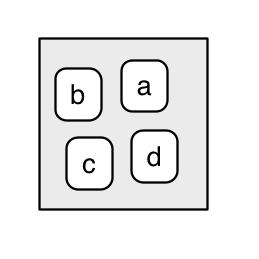
\includegraphics[width=1.18in]{diagrams/environments.png/bag-of-names.png}

Each name points to an object stored elsewhere in memory:

\begin{Shaded}
\begin{Highlighting}[]
\NormalTok{e <-}\StringTok{ }\KeywordTok{new.env}\NormalTok{()}
\NormalTok{e$a <-}\StringTok{ }\OtherTok{FALSE}
\NormalTok{e$b <-}\StringTok{ "a"}
\NormalTok{e$c <-}\StringTok{ }\FloatTok{2.3}
\NormalTok{e$d <-}\StringTok{ }\DecValTok{1}\NormalTok{:}\DecValTok{3}
\end{Highlighting}
\end{Shaded}

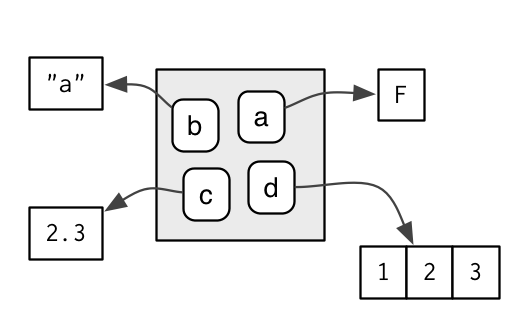
\includegraphics[width=2.36in]{diagrams/environments.png/bindings.png}

The objects don't live in the environment so multiple names can point to
the same object:

\begin{Shaded}
\begin{Highlighting}[]
\NormalTok{e$a <-}\StringTok{ }\NormalTok{e$d}
\end{Highlighting}
\end{Shaded}

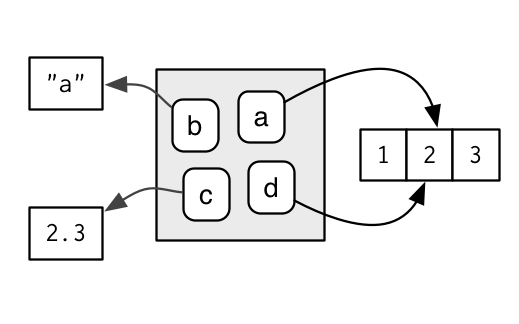
\includegraphics[width=2.36in]{diagrams/environments.png/multiple-names.png}

Confusingly they can also point to different objects that have the same
value:

\begin{Shaded}
\begin{Highlighting}[]
\NormalTok{e$a <-}\StringTok{ }\DecValTok{1}\NormalTok{:}\DecValTok{3}
\end{Highlighting}
\end{Shaded}

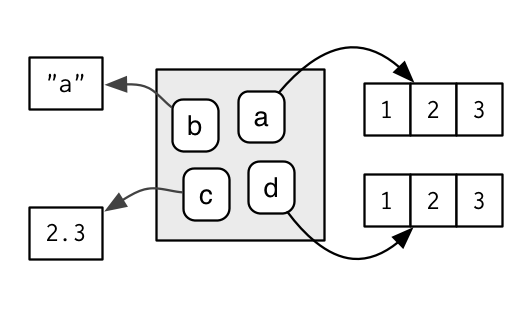
\includegraphics[width=2.36in]{diagrams/environments.png/copies.png}

If an object has no names pointing to it, it gets automatically deleted
by the garbage collector. This process is described in more detail in
\hyperref[gc]{gc}.

Every environment has a parent, another environment. In diagrams, I'll
represent the pointer to parent with a small black circle. The parent is
used to implement lexical scoping: if a name is not found in an
environment, then R will look in its parent (and so on). Only one
environment doesn't have a parent: the \textbf{empty} environment.
\index{environments!empty}

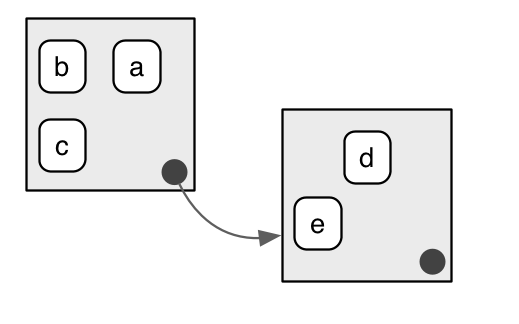
\includegraphics[width=2.36in]{diagrams/environments.png/parents.png}

We use the metaphor of a family to refer to environments. The
grandparent of an environment is the parent's parent, and the ancestors
include all parent environments up to the empty environment. It's rare
to talk about the children of an environment because there are no back
links: given an environment we have no way to find its children.

Generally, an environment is similar to a list, with four important
exceptions:

\begin{itemize}
\item
  Every object in an environment has a unique name.
\item
  The objects in an environment are not ordered (i.e., it doesn't make
  sense to ask what the first object in an environment is).
\item
  An environment has a parent.
\item
  Environments have reference semantics.
\end{itemize}

More technically, an environment is made up of two components, the
\textbf{frame}, which contains the name-object bindings (and behaves
much like a named list), and the parent environment. Unfortunately
``frame'' is used inconsistently in R. For example,
\texttt{parent.frame()} doesn't give you the parent frame of an
environment. Instead, it gives you the \emph{calling} environment. This
is discussed in more detail in \hyperref[calling-environments]{calling
environments}. \index{frames} \index{environments!parent}

There are four special environments:

\begin{itemize}
\item
  The \texttt{globalenv()}, or global environment, is the interactive
  workspace. This is the environment in which you normally work. The
  parent of the global environment is the last package that you attached
  with \texttt{library()} or \texttt{require()}.
\item
  The \texttt{baseenv()}, or base environment, is the environment of the
  base package. Its parent is the empty environment.
\item
  The \texttt{emptyenv()}, or empty environment, is the ultimate
  ancestor of all environments, and the only environment without a
  parent.
\item
  The \texttt{environment()} is the current environment.
\end{itemize}

\texttt{search()} lists all parents of the global environment. This is
called the search path because objects in these environments can be
found from the top-level interactive workspace. It contains one
environment for each attached package and any other objects that you've
\texttt{attach()}ed. It also contains a special environment called
\texttt{Autoloads} which is used to save memory by only loading package
objects (like big datasets) when needed. \indexc{search()}

You can access any environment on the search list using
\texttt{as.environment()}.

\begin{Shaded}
\begin{Highlighting}[]
\KeywordTok{search}\NormalTok{()}
\CommentTok{#> [1] ".GlobalEnv"        "package:stats"     "package:graphics" }
\CommentTok{#> [4] "package:grDevices" "package:utils"     "package:datasets" }
\CommentTok{#> [7] "package:methods"   "Autoloads"         "package:base"     }

\KeywordTok{as.environment}\NormalTok{(}\StringTok{"package:stats"}\NormalTok{)}
\CommentTok{#> <environment: package:stats>}
\end{Highlighting}
\end{Shaded}

\texttt{globalenv()}, \texttt{baseenv()}, the environments on the search
path, and \texttt{emptyenv()} are connected as shown below. Each time
you load a new package with \texttt{library()} it is inserted between
the global environment and the package that was previously at the top of
the search path.

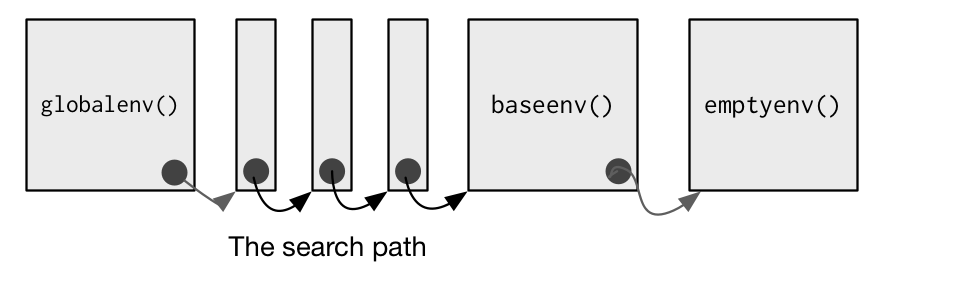
\includegraphics[width=4.35in]{diagrams/environments.png/search-path.png}

To create an environment manually, use \texttt{new.env()}. You can list
the bindings in the environment's frame with \texttt{ls()} and see its
parent with \texttt{parent.env()}. \index{environments!creating}

\begin{Shaded}
\begin{Highlighting}[]
\NormalTok{e <-}\StringTok{ }\KeywordTok{new.env}\NormalTok{()}
\CommentTok{# the default parent provided by new.env() is environment from }
\CommentTok{# which it is called - in this case that's the global environment.}
\KeywordTok{parent.env}\NormalTok{(e)}
\CommentTok{#> <environment: R_GlobalEnv>}
\KeywordTok{ls}\NormalTok{(e)}
\CommentTok{#> character(0)}
\end{Highlighting}
\end{Shaded}

The easiest way to modify the bindings in an environment is to treat it
like a list:

\begin{Shaded}
\begin{Highlighting}[]
\NormalTok{e$a <-}\StringTok{ }\DecValTok{1}
\NormalTok{e$b <-}\StringTok{ }\DecValTok{2}
\KeywordTok{ls}\NormalTok{(e)}
\CommentTok{#> [1] "a" "b"}
\NormalTok{e$a}
\CommentTok{#> [1] 1}
\end{Highlighting}
\end{Shaded}

By default, \texttt{ls()} only shows names that don't begin with
\texttt{.}. Use \texttt{all.names = TRUE} to show all bindings in an
environment: \indexc{ls()}

\begin{Shaded}
\begin{Highlighting}[]
\NormalTok{e$.a <-}\StringTok{ }\DecValTok{2}
\KeywordTok{ls}\NormalTok{(e)}
\CommentTok{#> [1] "a" "b"}
\KeywordTok{ls}\NormalTok{(e, }\DataTypeTok{all.names =} \OtherTok{TRUE}\NormalTok{)}
\CommentTok{#> [1] ".a" "a"  "b"}
\end{Highlighting}
\end{Shaded}

Another useful way to view an environment is \texttt{ls.str()}. It is
more useful than \texttt{str()} because it shows each object in the
environment. Like \texttt{ls()}, it also has an \texttt{all.names}
argument.

\begin{Shaded}
\begin{Highlighting}[]
\KeywordTok{str}\NormalTok{(e)}
\CommentTok{#> <environment: 0x7fba6aac1ad8>}
\KeywordTok{ls.str}\NormalTok{(e)}
\CommentTok{#> a :  num 1}
\CommentTok{#> b :  num 2}
\end{Highlighting}
\end{Shaded}

Given a name, you can extract the value to which it is bound with
\texttt{\$}, \texttt{{[}{[}}, or \texttt{get()}:

\begin{itemize}
\item
  \texttt{\$} and \texttt{{[}{[}} look only in one environment and
  return \texttt{NULL} if there is no binding associated with the name.
  \indexc{\$} \indexc{[[}
\item
  \texttt{get()} uses the regular scoping rules and throws an error if
  the binding is not found. \indexc{get()}
\end{itemize}

\begin{Shaded}
\begin{Highlighting}[]
\NormalTok{e$c <-}\StringTok{ }\DecValTok{3}
\NormalTok{e$c}
\CommentTok{#> [1] 3}
\NormalTok{e[[}\StringTok{"c"}\NormalTok{]]}
\CommentTok{#> [1] 3}
\KeywordTok{get}\NormalTok{(}\StringTok{"c"}\NormalTok{, }\DataTypeTok{envir =} \NormalTok{e)}
\CommentTok{#> [1] 3}
\end{Highlighting}
\end{Shaded}

Deleting objects from environments works a little differently from
lists. With a list you can remove an entry by setting it to
\texttt{NULL}. In environments, that will create a new binding to
\texttt{NULL}. Instead, use \texttt{rm()} to remove the binding.
\indexc{rm()} \index{environments!removing an element}

\begin{Shaded}
\begin{Highlighting}[]
\NormalTok{e <-}\StringTok{ }\KeywordTok{new.env}\NormalTok{()}

\NormalTok{e$a <-}\StringTok{ }\DecValTok{1}
\NormalTok{e$a <-}\StringTok{ }\OtherTok{NULL}
\KeywordTok{ls}\NormalTok{(e)}
\CommentTok{#> [1] "a"}

\KeywordTok{rm}\NormalTok{(}\StringTok{"a"}\NormalTok{, }\DataTypeTok{envir =} \NormalTok{e)}
\KeywordTok{ls}\NormalTok{(e)}
\CommentTok{#> character(0)}
\end{Highlighting}
\end{Shaded}

You can determine if a binding exists in an environment with
\texttt{exists()}. Like \texttt{get()}, its default behaviour is to
follow the regular scoping rules and look in parent environments. If you
don't want this behavior, use \texttt{inherits = FALSE}:

\begin{Shaded}
\begin{Highlighting}[]
\NormalTok{x <-}\StringTok{ }\DecValTok{10}
\KeywordTok{exists}\NormalTok{(}\StringTok{"x"}\NormalTok{, }\DataTypeTok{envir =} \NormalTok{e)}
\CommentTok{#> [1] TRUE}
\KeywordTok{exists}\NormalTok{(}\StringTok{"x"}\NormalTok{, }\DataTypeTok{envir =} \NormalTok{e, }\DataTypeTok{inherits =} \OtherTok{FALSE}\NormalTok{)}
\CommentTok{#> [1] FALSE}
\end{Highlighting}
\end{Shaded}

To compare environments, you must use \texttt{identical()} not
\texttt{==}:

\begin{Shaded}
\begin{Highlighting}[]
\KeywordTok{identical}\NormalTok{(}\KeywordTok{globalenv}\NormalTok{(), }\KeywordTok{environment}\NormalTok{())}
\CommentTok{#> [1] TRUE}
\KeywordTok{globalenv}\NormalTok{() ==}\StringTok{ }\KeywordTok{environment}\NormalTok{()}
\CommentTok{#> Error in globalenv() == environment(): comparison (1) is possible only for atomic and list types}
\end{Highlighting}
\end{Shaded}

\subsection{Exercises}

\begin{enumerate}
\def\labelenumi{\arabic{enumi}.}
\item
  List three ways in which an environment differs from a list.
\item
  If you don't supply an explicit environment, where do \texttt{ls()}
  and \texttt{rm()} look? Where does \texttt{\textless{}-} make
  bindings?
\item
  Using \texttt{parent.env()} and a loop (or a recursive function),
  verify that the ancestors of \texttt{globalenv()} include
  \texttt{baseenv()} and \texttt{emptyenv()}. Use the same basic idea to
  implement your own version of \texttt{search()}.
\end{enumerate}

\hyperdef{}{env-recursion}{\section{Recursing over
environments}\label{env-recursion}}

Environments form a tree, so it's often convenient to write a recursive
function. This section shows you how by applying your new knowledge of
environments to understand the helpful \texttt{pryr::where()}. Given a
name, \texttt{where()} finds the environment \emph{where} that name is
defined, using R's regular scoping rules:
\index{recursion!over environments}

\begin{Shaded}
\begin{Highlighting}[]
\KeywordTok{library}\NormalTok{(pryr)}
\NormalTok{x <-}\StringTok{ }\DecValTok{5}
\KeywordTok{where}\NormalTok{(}\StringTok{"x"}\NormalTok{)}
\CommentTok{#> <environment: R_GlobalEnv>}
\KeywordTok{where}\NormalTok{(}\StringTok{"mean"}\NormalTok{)}
\CommentTok{#> <environment: base>}
\end{Highlighting}
\end{Shaded}

The definition of \texttt{where()} is straightforward. It has two
arguments: the name to look for (as a string), and the environment in
which to start the search. (We'll learn later why
\texttt{parent.frame()} is a good default in
\hyperref[calling-environments]{calling environments}.)

\begin{Shaded}
\begin{Highlighting}[]
\NormalTok{where <-}\StringTok{ }\NormalTok{function(name, }\DataTypeTok{env =} \KeywordTok{parent.frame}\NormalTok{()) \{}
  \NormalTok{if (}\KeywordTok{identical}\NormalTok{(env, }\KeywordTok{emptyenv}\NormalTok{())) \{}
    \CommentTok{# Base case}
    \KeywordTok{stop}\NormalTok{(}\StringTok{"Can't find "}\NormalTok{, name, }\DataTypeTok{call. =} \OtherTok{FALSE}\NormalTok{)}
    
  \NormalTok{\} else if (}\KeywordTok{exists}\NormalTok{(name, }\DataTypeTok{envir =} \NormalTok{env, }\DataTypeTok{inherits =} \OtherTok{FALSE}\NormalTok{)) \{}
    \CommentTok{# Success case}
    \NormalTok{env}
    
  \NormalTok{\} else \{}
    \CommentTok{# Recursive case}
    \KeywordTok{where}\NormalTok{(name, }\KeywordTok{parent.env}\NormalTok{(env))}
    
  \NormalTok{\}}
\NormalTok{\}}
\end{Highlighting}
\end{Shaded}

There are three cases:

\begin{itemize}
\item
  The base case: we've reached the empty environment and haven't found
  the binding. We can't go any further, so we throw an error.
\item
  The successful case: the name exists in this environment, so we return
  the environment.
\item
  The recursive case: the name was not found in this environment, so try
  the parent.
\end{itemize}

It's easier to see what's going on with an example. Imagine you have two
environments as in the following diagram:

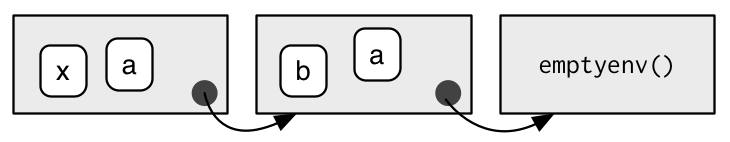
\includegraphics[width=3.32in]{diagrams/environments.png/where-ex.png}

\begin{itemize}
\item
  If you're looking for \texttt{a}, \texttt{where()} will find it in the
  first environment.
\item
  If you're looking for \texttt{b}, it's not in the first environment,
  so \texttt{where()} will look in its parent and find it there.
\item
  If you're looking for \texttt{c}, it's not in the first environment,
  or the second environment, so \texttt{where()} reaches the empty
  environment and throws an error.
\end{itemize}

It's natural to work with environments recursively, so \texttt{where()}
provides a useful template. Removing the specifics of \texttt{where()}
shows the structure more clearly:

\begin{Shaded}
\begin{Highlighting}[]
\NormalTok{f <-}\StringTok{ }\NormalTok{function(..., }\DataTypeTok{env =} \KeywordTok{parent.frame}\NormalTok{()) \{}
  \NormalTok{if (}\KeywordTok{identical}\NormalTok{(env, }\KeywordTok{emptyenv}\NormalTok{())) \{}
    \CommentTok{# base case}
  \NormalTok{\} else if (success) \{}
    \CommentTok{# success case}
  \NormalTok{\} else \{}
    \CommentTok{# recursive case}
    \KeywordTok{f}\NormalTok{(..., }\DataTypeTok{env =} \KeywordTok{parent.env}\NormalTok{(env))}
  \NormalTok{\}}
\NormalTok{\}}
\end{Highlighting}
\end{Shaded}

\begin{shortbox}\Boxhead{Iteration vs. recursion}

It's possible to use a loop instead of recursion. This might run
slightly faster (because we eliminate some function calls), but I think
it's harder to understand. I include it because you might find it easier
to see what's happening if you're less familiar with recursive
functions.

\begin{Shaded}
\begin{Highlighting}[]
\NormalTok{is_empty <-}\StringTok{ }\NormalTok{function(x) }\KeywordTok{identical}\NormalTok{(x, }\KeywordTok{emptyenv}\NormalTok{())}

\NormalTok{f2 <-}\StringTok{ }\NormalTok{function(..., }\DataTypeTok{env =} \KeywordTok{parent.frame}\NormalTok{()) \{}
  \NormalTok{while(!}\KeywordTok{is_empty}\NormalTok{(env)) \{}
    \NormalTok{if (success) \{}
      \CommentTok{# success case}
      \KeywordTok{return}\NormalTok{()}
    \NormalTok{\}}
    \CommentTok{# inspect parent}
    \NormalTok{env <-}\StringTok{ }\KeywordTok{parent.env}\NormalTok{(env)}
  \NormalTok{\}}

  \CommentTok{# base case}
\NormalTok{\}}
\end{Highlighting}
\end{Shaded}

\end{shortbox}

\subsection{Exercises}

\begin{enumerate}
\def\labelenumi{\arabic{enumi}.}
\item
  Modify \texttt{where()} to find all environments that contain a
  binding for \texttt{name}.
\item
  Write your own version of \texttt{get()} using a function written in
  the style of \texttt{where()}.
\item
  Write a function called \texttt{fget()} that finds only function
  objects. It should have two arguments, \texttt{name} and \texttt{env},
  and should obey the regular scoping rules for functions: if there's an
  object with a matching name that's not a function, look in the parent.
  For an added challenge, also add an \texttt{inherits} argument which
  controls whether the function recurses up the parents or only looks in
  one environment.
\item
  Write your own version of \texttt{exists(inherits = FALSE)} (Hint: use
  \texttt{ls()}.) Write a recursive version that behaves like
  \texttt{exists(inherits = TRUE)}.
\end{enumerate}

\hyperdef{}{function-envs}{\section{Function
environments}\label{function-envs}}

Most environments are not created by you with \texttt{new.env()} but are
created as a consequence of using functions. This section discusses the
four types of environments associated with a function: enclosing,
binding, execution, and calling. \index{functions!environments}

The \textbf{enclosing} environment is the environment where the function
was created. Every function has one and only one enclosing environment.
For the three other types of environment, there may be 0, 1, or many
environments associated with each function:

\begin{itemize}
\item
  Binding a function to a name with \texttt{\textless{}-} defines a
  \textbf{binding} environment.
\item
  Calling a function creates an ephemeral \textbf{execution} environment
  that stores variables created during execution.
\item
  Every execution environment is associated with a \textbf{calling}
  environment, which tells you where the function was called.
\end{itemize}

The following sections will explain why each of these environments is
important, how to access them, and how you might use them.

\subsection{The enclosing environment}

When a function is created, it gains a reference to the environment
where it was made. This is the \textbf{enclosing environment} and is
used for lexical scoping. You can determine the enclosing environment of
a function by calling \texttt{environment()} with a function as its
first argument: \index{environments!enclosing}

\begin{Shaded}
\begin{Highlighting}[]
\NormalTok{y <-}\StringTok{ }\DecValTok{1}
\NormalTok{f <-}\StringTok{ }\NormalTok{function(x) x +}\StringTok{ }\NormalTok{y}
\KeywordTok{environment}\NormalTok{(f)}
\CommentTok{#> <environment: R_GlobalEnv>}
\end{Highlighting}
\end{Shaded}

In diagrams, I'll depict functions as rounded rectangles. The enclosing
environment of a function is given by a small black circle:

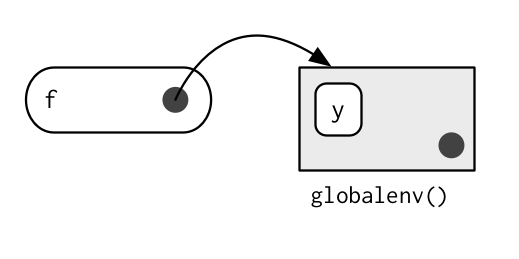
\includegraphics[width=2.06in]{diagrams/environments.png/enclosing.png}

\subsection{Binding environments}

The previous diagram is too simple because functions don't have names.
Instead, the name of a function is defined by a binding. The binding
environments of a function are all the environments which have a binding
to it. The following diagram better reflects this relationship because
the enclosing environment contains a binding from \texttt{f} to the
function: \index{environments!binding names}

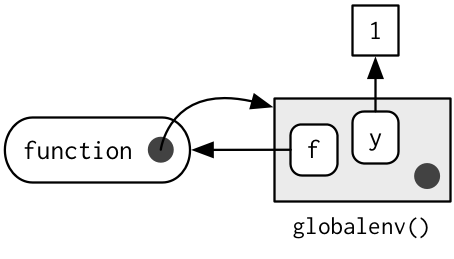
\includegraphics[width=2.06in]{diagrams/environments.png/binding.png}

In this case the enclosing and binding environments are the same. They
will be different if you assign a function into a different environment:

\begin{Shaded}
\begin{Highlighting}[]
\NormalTok{e <-}\StringTok{ }\KeywordTok{new.env}\NormalTok{()}
\NormalTok{e$g <-}\StringTok{ }\NormalTok{function() }\DecValTok{1}
\end{Highlighting}
\end{Shaded}

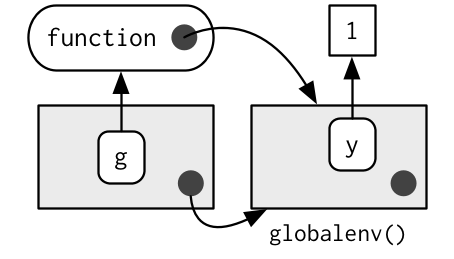
\includegraphics[width=2.06in]{diagrams/environments.png/binding-2.png}

The enclosing environment belongs to the function, and never changes,
even if the function is moved to a different environment. The enclosing
environment determines how the function finds values; the binding
environments determine how we find the function.

The distinction between the binding environment and the enclosing
environment is important for package namespaces. Package namespaces keep
packages independent. For example, if package A uses the base
\texttt{mean()} function, what happens if package B creates its own
\texttt{mean()} function? Namespaces ensure that package A continues to
use the base \texttt{mean()} function, and that package A is not
affected by package B (unless explicitly asked for). \index{namespaces}

Namespaces are implemented using environments, taking advantage of the
fact that functions don't have to live in their enclosing environments.
For example, take the base function \texttt{sd()}. It's binding and
enclosing environments are different:

\begin{Shaded}
\begin{Highlighting}[]
\KeywordTok{environment}\NormalTok{(sd)}
\CommentTok{#> <environment: namespace:stats>}
\KeywordTok{where}\NormalTok{(}\StringTok{"sd"}\NormalTok{)}
\CommentTok{#> <environment: package:stats>}
\end{Highlighting}
\end{Shaded}

The definition of \texttt{sd()} uses \texttt{var()}, but if we make our
own version of \texttt{var()} it doesn't affect \texttt{sd()}:

\begin{Shaded}
\begin{Highlighting}[]
\NormalTok{x <-}\StringTok{ }\DecValTok{1}\NormalTok{:}\DecValTok{10}
\KeywordTok{sd}\NormalTok{(x)}
\CommentTok{#> [1] 3.03}
\NormalTok{var <-}\StringTok{ }\NormalTok{function(x, }\DataTypeTok{na.rm =} \OtherTok{TRUE}\NormalTok{) }\DecValTok{100}
\KeywordTok{sd}\NormalTok{(x)}
\CommentTok{#> [1] 3.03}
\end{Highlighting}
\end{Shaded}

This works because every package has two environments associated with
it: the \emph{package} environment and the \emph{namespace} environment.
The package environment contains every publicly accessible function, and
is placed on the search path. The namespace environment contains all
functions (including internal functions), and its parent environment is
a special imports environment that contains bindings to all the
functions that the package needs. Every exported function in a package
is bound into the \emph{package} environment, but enclosed by the
\emph{namespace} environment. This complicated relationship is
illustrated by the following diagram:

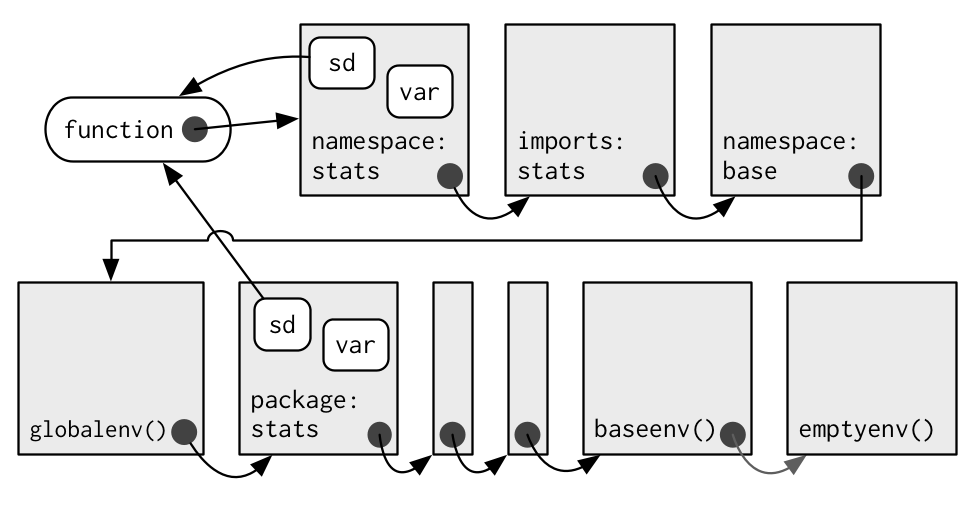
\includegraphics[width=4.35in]{diagrams/environments.png/namespace.png}

When we type \texttt{var} into the console, it's found first in the
global environment. When \texttt{sd()} looks for \texttt{var()} it finds
it first in its namespace environment so never looks in the
\texttt{globalenv()}.

\subsection{Execution environments}

What will the following function return the first time it's run? What
about the second? \index{environments!execution}

\begin{Shaded}
\begin{Highlighting}[]
\NormalTok{g <-}\StringTok{ }\NormalTok{function(x) \{}
  \NormalTok{if (!}\KeywordTok{exists}\NormalTok{(}\StringTok{"a"}\NormalTok{, }\DataTypeTok{inherits =} \OtherTok{FALSE}\NormalTok{)) \{}
    \KeywordTok{message}\NormalTok{(}\StringTok{"Defining a"}\NormalTok{)}
    \NormalTok{a <-}\StringTok{ }\DecValTok{1}
  \NormalTok{\} else \{}
    \NormalTok{a <-}\StringTok{ }\NormalTok{a +}\StringTok{ }\DecValTok{1}
  \NormalTok{\}}
  \NormalTok{a}
\NormalTok{\}}
\KeywordTok{g}\NormalTok{(}\DecValTok{10}\NormalTok{)}
\KeywordTok{g}\NormalTok{(}\DecValTok{10}\NormalTok{)}
\end{Highlighting}
\end{Shaded}

This function returns the same value every time it is called because of
the fresh start principle, described in \hyperref[fresh-start]{a fresh
start}. Each time a function is called, a new environment is created to
host execution. The parent of the execution environment is the enclosing
environment of the function. Once the function has completed, this
environment is thrown away.

Let's depict that graphically with a simpler function. I draw execution
environments around the function they belong to with a dotted border.

\begin{Shaded}
\begin{Highlighting}[]
\NormalTok{h <-}\StringTok{ }\NormalTok{function(x) \{}
  \NormalTok{a <-}\StringTok{ }\DecValTok{2}
  \NormalTok{x +}\StringTok{ }\NormalTok{a}
\NormalTok{\}}
\NormalTok{y <-}\StringTok{ }\KeywordTok{h}\NormalTok{(}\DecValTok{1}\NormalTok{)}
\end{Highlighting}
\end{Shaded}

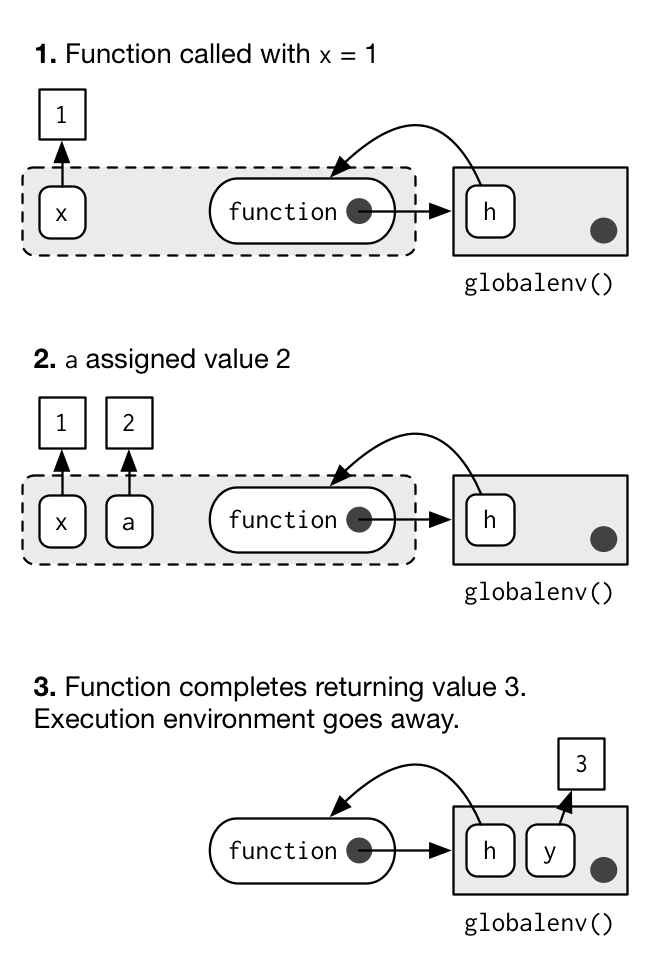
\includegraphics[width=2.95in]{diagrams/environments.png/execution.png}

When you create a function inside another function, the enclosing
environment of the child function is the execution environment of the
parent, and the execution environment is no longer ephemeral. The
following example illustrates that idea with a function factory,
\texttt{plus()}. We use that factory to create a function called
\texttt{plus\_one()}. The enclosing environment of \texttt{plus\_one()}
is the execution environment of \texttt{plus()} where \texttt{x} is
bound to the value 1. \index{closures|environment}

\begin{Shaded}
\begin{Highlighting}[]
\NormalTok{plus <-}\StringTok{ }\NormalTok{function(x) \{}
  \NormalTok{function(y) x +}\StringTok{ }\NormalTok{y}
\NormalTok{\}}
\NormalTok{plus_one <-}\StringTok{ }\KeywordTok{plus}\NormalTok{(}\DecValTok{1}\NormalTok{)}
\KeywordTok{identical}\NormalTok{(}\KeywordTok{parent.env}\NormalTok{(}\KeywordTok{environment}\NormalTok{(plus_one)), }\KeywordTok{environment}\NormalTok{(plus))}
\CommentTok{#> [1] TRUE}
\end{Highlighting}
\end{Shaded}

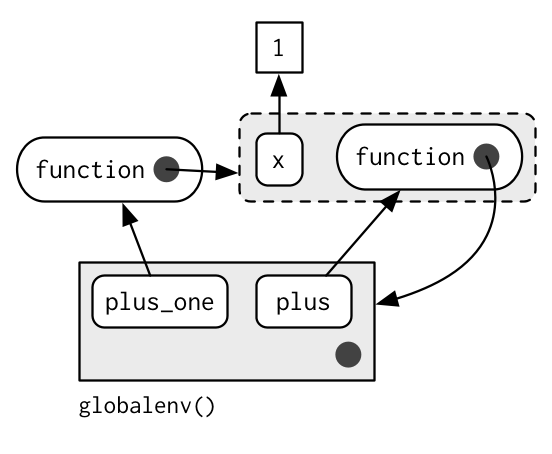
\includegraphics[width=2.51in]{diagrams/environments.png/closure-2.png}

You'll learn more about function factories in
\hyperref[functional-programming]{functional programming}.

\hyperdef{}{calling-environments}{\subsection{Calling
environments}\label{calling-environments}}

Look at the following code. What do you expect \texttt{i()} to return
when the code is run? \index{environments|calling}

\begin{Shaded}
\begin{Highlighting}[]
\NormalTok{h <-}\StringTok{ }\NormalTok{function() \{}
  \NormalTok{x <-}\StringTok{ }\DecValTok{10}
  \NormalTok{function() \{}
    \NormalTok{x}
  \NormalTok{\}}
\NormalTok{\}}
\NormalTok{i <-}\StringTok{ }\KeywordTok{h}\NormalTok{()}
\NormalTok{x <-}\StringTok{ }\DecValTok{20}
\KeywordTok{i}\NormalTok{()}
\end{Highlighting}
\end{Shaded}

The top-level \texttt{x} (bound to 20) is a red herring: using the
regular scoping rules, \texttt{h()} looks first where it is defined and
finds that the value associated with \texttt{x} is 10. However, it's
still meaningful to ask what value \texttt{x} is associated within the
environment where \texttt{i()} is called: \texttt{x} is 10 in the
environment where \texttt{h()} is defined, but it is 20 in the
environment where \texttt{h()} is called.

We can access this environment using the unfortunately named
\texttt{parent.frame()}. This function returns the \textbf{environment}
where the function was called. We can also use this function to look up
the value of names in that environment:

\begin{Shaded}
\begin{Highlighting}[]
\NormalTok{f2 <-}\StringTok{ }\NormalTok{function() \{}
  \NormalTok{x <-}\StringTok{ }\DecValTok{10}
  \NormalTok{function() \{}
    \NormalTok{def <-}\StringTok{ }\KeywordTok{get}\NormalTok{(}\StringTok{"x"}\NormalTok{, }\KeywordTok{environment}\NormalTok{())}
    \NormalTok{cll <-}\StringTok{ }\KeywordTok{get}\NormalTok{(}\StringTok{"x"}\NormalTok{, }\KeywordTok{parent.frame}\NormalTok{())}
    \KeywordTok{list}\NormalTok{(}\DataTypeTok{defined =} \NormalTok{def, }\DataTypeTok{called =} \NormalTok{cll)}
  \NormalTok{\}}
\NormalTok{\}}
\NormalTok{g2 <-}\StringTok{ }\KeywordTok{f2}\NormalTok{()}
\NormalTok{x <-}\StringTok{ }\DecValTok{20}
\KeywordTok{str}\NormalTok{(}\KeywordTok{g2}\NormalTok{())}
\CommentTok{#> List of 2}
\CommentTok{#>  $ defined: num 10}
\CommentTok{#>  $ called : num 20}
\end{Highlighting}
\end{Shaded}

In more complicated scenarios, there's not just one parent call, but a
sequence of calls which lead all the way back to the initiating
function, called from the top-level. The following code generates a call
stack three levels deep. The open-ended arrows represent the calling
environment of each execution environment.

\begin{Shaded}
\begin{Highlighting}[]
\NormalTok{x <-}\StringTok{ }\DecValTok{0}
\NormalTok{y <-}\StringTok{ }\DecValTok{10}
\NormalTok{f <-}\StringTok{ }\NormalTok{function() \{}
  \NormalTok{x <-}\StringTok{ }\DecValTok{1}
  \KeywordTok{g}\NormalTok{()}
\NormalTok{\}}
\NormalTok{g <-}\StringTok{ }\NormalTok{function() \{}
  \NormalTok{x <-}\StringTok{ }\DecValTok{2}
  \KeywordTok{h}\NormalTok{()}
\NormalTok{\}}
\NormalTok{h <-}\StringTok{ }\NormalTok{function() \{}
  \NormalTok{x <-}\StringTok{ }\DecValTok{3}
  \NormalTok{x +}\StringTok{ }\NormalTok{y}
\NormalTok{\}}
\KeywordTok{f}\NormalTok{()}
\CommentTok{#> [1] 13}
\end{Highlighting}
\end{Shaded}

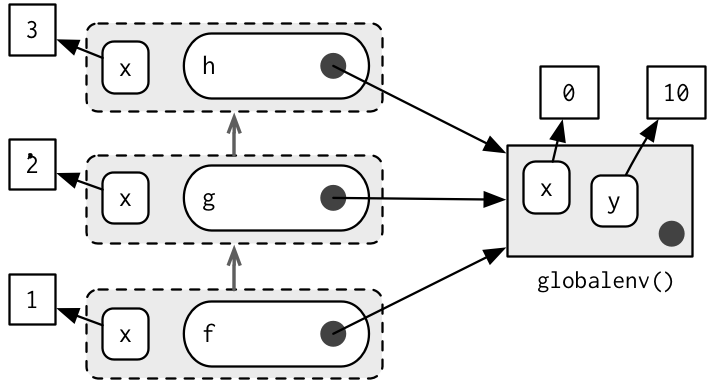
\includegraphics[width=3.25in]{diagrams/environments.png/calling.png}

Note that each execution environment has two parents: a calling
environment and an enclosing environment. R's regular scoping rules only
use the enclosing parent; \texttt{parent.frame()} allows you to access
the calling parent.

Looking up variables in the calling environment rather than in the
enclosing environment is called \textbf{dynamic scoping}. Few languages
implement dynamic scoping (Emacs Lisp is a
\href{http://www.gnu.org/software/emacs/emacs-paper.html\#SEC15}{notable
exception}.) This is because dynamic scoping makes it much harder to
reason about how a function operates: not only do you need to know how
it was defined, you also need to know in what context it was called.
Dynamic scoping is primarily useful for developing functions that aid
interactive data analysis. It is one of the topics discussed in
\hyperref[nse]{non-standard evaluation}. \index{scoping!dynamic}
\index{dynamic scoping}

\subsection{Exercises}

\begin{enumerate}
\def\labelenumi{\arabic{enumi}.}
\item
  List the four environments associated with a function. What does each
  one do? Why is the distinction between enclosing and binding
  environments particularly important?
\item
  Draw a diagram that shows the enclosing environments of this function:

\begin{Shaded}
\begin{Highlighting}[]
\NormalTok{f1 <-}\StringTok{ }\NormalTok{function(x1) \{}
  \NormalTok{f2 <-}\StringTok{ }\NormalTok{function(x2) \{}
    \NormalTok{f3 <-}\StringTok{ }\NormalTok{function(x3) \{}
      \NormalTok{x1 +}\StringTok{ }\NormalTok{x2 +}\StringTok{ }\NormalTok{x3}
    \NormalTok{\}}
    \KeywordTok{f3}\NormalTok{(}\DecValTok{3}\NormalTok{)}
  \NormalTok{\}}
  \KeywordTok{f2}\NormalTok{(}\DecValTok{2}\NormalTok{)}
\NormalTok{\}}
\KeywordTok{f1}\NormalTok{(}\DecValTok{1}\NormalTok{)}
\end{Highlighting}
\end{Shaded}
\item
  Expand your previous diagram to show function bindings.
\item
  Expand it again to show the execution and calling environments.
\item
  Write an enhanced version of \texttt{str()} that provides more
  information about functions. Show where the function was found and
  what environment it was defined in.
\end{enumerate}

\hyperdef{}{binding}{\section{Binding names to values}\label{binding}}

Assignment is the act of binding (or rebinding) a name to a value in an
environment. It is the counterpart to scoping, the set of rules that
determines how to find the value associated with a name. Compared to
most languages, R has extremely flexible tools for binding names to
values. In fact, you can not only bind values to names, but you can also
bind expressions (promises) or even functions, so that every time you
access the value associated with a name, you get something different!
\index{bindings}

You've probably used regular assignment in R thousands of times. Regular
assignment creates a binding between a name and an object in the current
environment. Names usually consist of letters, digits, \texttt{.} and
\texttt{\_}, and can't begin with \texttt{\_}. If you try to use a name
that doesn't follow these rules, you get an error:

\begin{Shaded}
\begin{Highlighting}[]
\NormalTok{_abc <-}\StringTok{ }\DecValTok{1}
\CommentTok{# Error: unexpected input in "_"}
\end{Highlighting}
\end{Shaded}

Reserved words (like \texttt{TRUE}, \texttt{NULL}, \texttt{if}, and
\texttt{function}) follow the rules but are reserved by R for other
purposes:

\begin{Shaded}
\begin{Highlighting}[]
\NormalTok{if <-}\StringTok{ }\DecValTok{10}
\CommentTok{#> Error: unexpected assignment in "if <-"}
\end{Highlighting}
\end{Shaded}

A complete list of reserved words can be found in \texttt{?Reserved}.
\index{reserved names} \indexc{`} \index{non-syntactic names}

It's possible to override the usual rules and use a name with any
sequence of characters by surrounding the name with backticks:

\begin{Shaded}
\begin{Highlighting}[]
\StringTok{`}\DataTypeTok{a + b}\StringTok{`} \NormalTok{<-}\StringTok{ }\DecValTok{3}
\StringTok{`}\DataTypeTok{:)}\StringTok{`} \NormalTok{<-}\StringTok{ "smile"}
\StringTok{`}\DataTypeTok{    }\StringTok{`} \NormalTok{<-}\StringTok{ "spaces"}
\KeywordTok{ls}\NormalTok{()}
\CommentTok{#  [1] "    "   ":)"     "a + b"}
\StringTok{`}\DataTypeTok{:)}\StringTok{`}
\CommentTok{#  [1] "smile"}
\end{Highlighting}
\end{Shaded}

\begin{shortbox}\Boxhead{Quotes}

You can also create non-syntactic bindings using single and double
quotes instead of backticks, but I don't recommend it. The ability to
use strings on the left hand side of the assignment arrow is a
historical artefact, used before R supported backticks.

\end{shortbox}

The regular assignment arrow, \texttt{\textless{}-}, always creates a
variable in the current environment. The deep assignment arrow,
\texttt{\textless{}\textless{}-}, never creates a variable in the
current environment, but instead modifies an existing variable found by
walking up the parent environments. You can also do deep binding with
\texttt{assign()}: \texttt{name \textless{}\textless{}- value} is
equivalent to \texttt{assign("name", value, inherits = TRUE)}.

\begin{Shaded}
\begin{Highlighting}[]
\NormalTok{x <-}\StringTok{ }\DecValTok{0}
\NormalTok{f <-}\StringTok{ }\NormalTok{function() \{}
  \NormalTok{x <<-}\StringTok{ }\DecValTok{1}
\NormalTok{\}}
\KeywordTok{f}\NormalTok{()}
\NormalTok{x}
\CommentTok{#> [1] 1}
\end{Highlighting}
\end{Shaded}

If \texttt{\textless{}\textless{}-} doesn't find an existing variable,
it will create one in the global environment. This is usually
undesirable, because global variables introduce non-obvious dependencies
between functions. \texttt{\textless{}\textless{}-} is most often used
in conjunction with a closure, as described in
\hyperref[closures]{Closures}.

There are two other special types of binding, delayed and active:

\begin{itemize}
\item
  Rather than assigning the result of an expression immediately, a
  \textbf{delayed binding} creates and stores a promise to evaluate the
  expression when needed. We can create delayed bindings with the
  special assignment operator \texttt{\%\textless{}d-\%}, provided by
  the pryr package.

\begin{Shaded}
\begin{Highlighting}[]
\KeywordTok{library}\NormalTok{(pryr)}
\KeywordTok{system.time}\NormalTok{(b %<d-%}\StringTok{ }\NormalTok{\{}\KeywordTok{Sys.sleep}\NormalTok{(}\DecValTok{1}\NormalTok{); }\DecValTok{1}\NormalTok{\})}
\CommentTok{#>    user  system elapsed }
\CommentTok{#>   0.000   0.000   0.001}
\KeywordTok{system.time}\NormalTok{(b)}
\CommentTok{#>    user  system elapsed }
\CommentTok{#>   0.000   0.000   1.001}
\end{Highlighting}
\end{Shaded}

  \texttt{\%\textless{}d-\%} is a wrapper around the base
  \texttt{delayedAssign()} function, which you may need to use directly
  if you need more control. Delayed bindings are used to implement
  \texttt{autoload()}, which makes R behave as if the package data is in
  memory, even though it's only loaded from disk when you ask for it.
  \index{bindings!delayed}
\item
  \textbf{Active} are not bound to a constant object. Instead, they're
  re-computed every time they're accessed:

\begin{Shaded}
\begin{Highlighting}[]
\NormalTok{x %<a-%}\StringTok{ }\KeywordTok{runif}\NormalTok{(}\DecValTok{1}\NormalTok{)}
\NormalTok{x}
\CommentTok{#> [1] 0.0808}
\NormalTok{x}
\CommentTok{#> [1] 0.834}
\KeywordTok{rm}\NormalTok{(x)}
\end{Highlighting}
\end{Shaded}

  \texttt{\%\textless{}a-\%} is a wrapper for the base function
  \texttt{makeActiveBinding()}. You may want to use this function
  directly if you want more control. Active bindings are used to
  implement reference class fields. \index{bindings!active}
\end{itemize}

\subsection{Exercises}

\begin{enumerate}
\def\labelenumi{\arabic{enumi}.}
\item
  What does this function do? How does it differ from
  \texttt{\textless{}\textless{}-} and why might you prefer it?

\begin{Shaded}
\begin{Highlighting}[]
\NormalTok{rebind <-}\StringTok{ }\NormalTok{function(name, value, }\DataTypeTok{env =} \KeywordTok{parent.frame}\NormalTok{()) \{}
  \NormalTok{if (}\KeywordTok{identical}\NormalTok{(env, }\KeywordTok{emptyenv}\NormalTok{())) \{}
    \KeywordTok{stop}\NormalTok{(}\StringTok{"Can't find "}\NormalTok{, name, }\DataTypeTok{call. =} \OtherTok{FALSE}\NormalTok{)}
  \NormalTok{\} else if (}\KeywordTok{exists}\NormalTok{(name, }\DataTypeTok{envir =} \NormalTok{env, }\DataTypeTok{inherits =} \OtherTok{FALSE}\NormalTok{)) \{}
    \KeywordTok{assign}\NormalTok{(name, value, }\DataTypeTok{envir =} \NormalTok{env)}
  \NormalTok{\} else \{}
    \KeywordTok{rebind}\NormalTok{(name, value, }\KeywordTok{parent.env}\NormalTok{(env))}
  \NormalTok{\}}
\NormalTok{\}}
\KeywordTok{rebind}\NormalTok{(}\StringTok{"a"}\NormalTok{, }\DecValTok{10}\NormalTok{)}
\CommentTok{#> Error: Can't find a}
\NormalTok{a <-}\StringTok{ }\DecValTok{5}
\KeywordTok{rebind}\NormalTok{(}\StringTok{"a"}\NormalTok{, }\DecValTok{10}\NormalTok{)}
\NormalTok{a}
\CommentTok{#> [1] 10}
\end{Highlighting}
\end{Shaded}
\item
  Create a version of \texttt{assign()} that will only bind new names,
  never re-bind old names. Some programming languages only do this, and
  are known as
  \href{http://en.wikipedia.org/wiki/Assignment_(computer_science)\#Single_assignment}{single
  assignment languages}.
\item
  Write an assignment function that can do active, delayed, and locked
  bindings. What might you call it? What arguments should it take? Can
  you guess which sort of assignment it should do based on the input?
\end{enumerate}

\hyperdef{}{explicit-envs}{\section{Explicit
environments}\label{explicit-envs}}

As well as powering scoping, environments are also useful data
structures in their own right because they have \textbf{reference
semantics}. Unlike most objects in R, when you modify an environment, it
does not make a copy. For example, look at this \texttt{modify()}
function. \index{copy-on-modify!exceptions} \index{reference semantics}

\begin{Shaded}
\begin{Highlighting}[]
\NormalTok{modify <-}\StringTok{ }\NormalTok{function(x) \{}
  \NormalTok{x$a <-}\StringTok{ }\DecValTok{2}
  \KeywordTok{invisible}\NormalTok{()}
\NormalTok{\}}
\end{Highlighting}
\end{Shaded}

If you apply it to a list, the original list is not changed because
modifying a list actually creates and modifies a copy.

\begin{Shaded}
\begin{Highlighting}[]
\NormalTok{x_l <-}\StringTok{ }\KeywordTok{list}\NormalTok{()}
\NormalTok{x_l$a <-}\StringTok{ }\DecValTok{1}
\KeywordTok{modify}\NormalTok{(x_l)}
\NormalTok{x_l$a}
\CommentTok{#> [1] 1}
\end{Highlighting}
\end{Shaded}

However, if you apply it to an environment, the original environment
\emph{is} modified:

\begin{Shaded}
\begin{Highlighting}[]
\NormalTok{x_e <-}\StringTok{ }\KeywordTok{new.env}\NormalTok{()}
\NormalTok{x_e$a <-}\StringTok{ }\DecValTok{1}
\KeywordTok{modify}\NormalTok{(x_e)}
\NormalTok{x_e$a}
\CommentTok{#> [1] 2}
\end{Highlighting}
\end{Shaded}

Just as you can use a list to pass data between functions, you can also
use an environment. When creating your own environment, note that you
should set its parent environment to be the empty environment. This
ensures you don't accidentally inherit objects from somewhere else:

\begin{Shaded}
\begin{Highlighting}[]
\NormalTok{x <-}\StringTok{ }\DecValTok{1}
\NormalTok{e1 <-}\StringTok{ }\KeywordTok{new.env}\NormalTok{()}
\KeywordTok{get}\NormalTok{(}\StringTok{"x"}\NormalTok{, }\DataTypeTok{envir =} \NormalTok{e1)}
\CommentTok{#> [1] 1}

\NormalTok{e2 <-}\StringTok{ }\KeywordTok{new.env}\NormalTok{(}\DataTypeTok{parent =} \KeywordTok{emptyenv}\NormalTok{())}
\KeywordTok{get}\NormalTok{(}\StringTok{"x"}\NormalTok{, }\DataTypeTok{envir =} \NormalTok{e2)}
\CommentTok{#> Error in get("x", envir = e2): object 'x' not found}
\end{Highlighting}
\end{Shaded}

Environments are data structures useful for solving three common
problems:

\begin{itemize}
\itemsep1pt\parskip0pt\parsep0pt
\item
  Avoiding copies of large data.
\item
  Managing state within a package.
\item
  Efficiently looking up values from names.
\end{itemize}

These are described in turn below.

\subsection{Avoiding copies}

Since environments have reference semantics, you'll never accidentally
create a copy. This makes it a useful vessel for large objects. It's a
common technique for bioconductor packages which often have to manage
large genomic objects. Changes to R 3.1.0 have made this use
substantially less important because modifying a list no longer makes a
deep copy. Previously, modifying a single element of a list would cause
every element to be copied, an expensive operation if some elements are
large. Now, modifying a list efficiently reuses existing vectors, saving
much time.

\subsection{Package state}

Explicit environments are useful in packages because they allow you to
maintain state across function calls. Normally, objects in a package are
locked, so you can't modify them directly. Instead, you can do something
like this:

\begin{Shaded}
\begin{Highlighting}[]
\NormalTok{my_env <-}\StringTok{ }\KeywordTok{new.env}\NormalTok{(}\DataTypeTok{parent =} \KeywordTok{emptyenv}\NormalTok{())}
\NormalTok{my_env$a <-}\StringTok{ }\DecValTok{1}

\NormalTok{get_a <-}\StringTok{ }\NormalTok{function() \{}
  \NormalTok{my_env$a}
\NormalTok{\}}
\NormalTok{set_a <-}\StringTok{ }\NormalTok{function(value) \{}
  \NormalTok{old <-}\StringTok{ }\NormalTok{my_env$a}
  \NormalTok{my_env$a <-}\StringTok{ }\NormalTok{value}
  \KeywordTok{invisible}\NormalTok{(old)}
\NormalTok{\}}
\end{Highlighting}
\end{Shaded}

Returning the old value from setter functions is a good pattern because
it makes it easier to reset the previous value in conjunction with
\texttt{on.exit()} (see more in \hyperref[on-exit]{on exit}).

\subsection{As a hashmap}

A hashmap is a data structure that takes constant, O(1), time to find an
object based on its name. Environments provide this behaviour by
default, so can be used to simulate a hashmap. See the CRAN package
\texttt{hash} for a complete development of this idea. \index{hashmaps}
\index{dictionaries}

\hyperdef{}{env-answers}{\section{Quiz answers}\label{env-answers}}

\begin{enumerate}
\def\labelenumi{\arabic{enumi}.}
\item
  There are four ways: every object in an environment must have a name;
  order doesn't matter; environments have parents; environments have
  reference semantics.
\item
  The parent of the global environment is the last package that you
  loaded. The only environment that doesn't have a parent is the empty
  environment.
\item
  The enclosing environment of a function is the environment where it
  was created. It determines where a function looks for variables.
\item
  Use \texttt{parent.frame()}.
\item
  \texttt{\textless{}-} always creates a binding in the current
  environment; \texttt{\textless{}\textless{}-} rebinds an existing name
  in a parent of the current environment.
\end{enumerate}

\chapter{Debugging, condition handling, and defensive
programming}\label{debugging}

What happens when something goes wrong with your R code? What do you do?
What tools do you have to address the problem? This chapter will teach
you how to fix unanticipated problems (debugging), show you how
functions can communicate problems and how you can take action based on
those communications (condition handling), and teach you how to avoid
common problems before they occur (defensive programming).

Debugging is the art and science of fixing unexpected problems in your
code. In this section you'll learn the tools and techniques that help
you get to the root cause of an error. You'll learn general strategies
for debugging, useful R functions like \texttt{traceback()} and
\texttt{browser()}, and interactive tools in RStudio.

Not all problems are unexpected. When writing a function, you can often
anticipate potential problems (like a non-existent file or the wrong
type of input). Communicating these problems to the user is the job of
\textbf{conditions}: errors, warnings, and messages.

\begin{itemize}
\item
  Fatal errors are raised by \texttt{stop()} and force all execution to
  terminate. Errors are used when there is no way for a function to
  continue. \index{errors} \indexc{stop()}
\item
  Warnings are generated by \texttt{warning()} and are used to display
  potential problems, such as when some elements of a vectorised input
  are invalid, like \texttt{log(-1:2)}.
\item
  Messages are generated by \texttt{message()} and are used to give
  informative output in a way that can easily be suppressed by the user
  (\texttt{?suppressMessages()}). I often use messages to let the user
  know what value the function has chosen for an important missing
  argument.
\end{itemize}

Conditions are usually displayed prominently, in a bold font or coloured
red depending on your R interface. You can tell them apart because
errors always start with ``Error'' and warnings with ``Warning
message''. Function authors can also communicate with their users with
\texttt{print()} or \texttt{cat()}, but I think that's a bad idea
because it's hard to capture and selectively ignore this sort of output.
Printed output is not a condition, so you can't use any of the useful
condition handling tools you'll learn about below.

Condition handling tools, like \texttt{withCallingHandlers()},
\texttt{tryCatch()}, and \texttt{try()} allow you to take specific
actions when a condition occurs. For example, if you're fitting many
models, you might want to continue fitting the others even if one fails
to converge. R offers an exceptionally powerful condition handling
system based on ideas from Common Lisp, but it's currently not very well
documented or often used. This chapter will introduce you to the most
important basics, but if you want to learn more, I recommend the
following two sources:

\begin{itemize}
\item
  \href{http://homepage.stat.uiowa.edu/~luke/R/exceptions/simpcond.html}{\emph{A
  prototype of a condition system for R}} by Robert Gentleman and Luke
  Tierney. This describes an early version of R's condition system.
  While the implementation has changed somewhat since this document was
  written, it provides a good overview of how the pieces fit together,
  and some motivation for its design.
\item
  \href{http://www.gigamonkeys.com/book/beyond-exception-handling-conditions-and-restarts.html}{\emph{Beyond
  Exception Handling: Conditions and Restarts}} by Peter Seibel. This
  describes exception handling in Lisp, which happens to be very similar
  to R's approach. It provides useful motivation and more sophisticated
  examples. I have provided an R translation of the chapter at
  \url{http://adv-r.had.co.nz/beyond-exception-handling.html}.
\end{itemize}

The chapter concludes with a discussion of ``defensive'' programming:
ways to avoid common errors before they occur. In the short run you'll
spend more time writing code, but in the long run you'll save time
because error messages will be more informative and will let you narrow
in on the root cause more quickly. The basic principle of defensive
programming is to ``fail fast'', to raise an error as soon as something
goes wrong. In R, this takes three particular forms: checking that
inputs are correct, avoiding non-standard evaluation, and avoiding
functions that can return different types of output.

\paragraph{Quiz}

Want to skip this chapter? Go for it, if you can answer the questions
below. Find the answers at the end of the chapter in
\hyperref[debugging-answers]{answers}.

\begin{enumerate}
\def\labelenumi{\arabic{enumi}.}
\item
  How can you find out where an error occured?
\item
  What does \texttt{browser()} do? List the five useful single-key
  commands that you can use inside of a \texttt{browser()} environment.
\item
  What function do you use to ignore errors in block of code?
\item
  Why might you want to create an error with a custom S3 class?
\end{enumerate}

\paragraph{Outline}

\begin{enumerate}
\def\labelenumi{\arabic{enumi}.}
\item
  \hyperref[debugging-techniques]{Debugging techniques} outlines a
  general approach for finding and resolving bugs.
\item
  \hyperref[debugging-tools]{Debugging tools} introduces you to the R
  functions and Rstudio features that help you locate exactly where an
  error occurred.
\item
  \hyperref[condition-handling]{Condition handling} shows you how you
  can catch conditions (errors, warnings, and messages) in your own
  code. This allows you to create code that's both more robust and more
  informative in the presence of errors.
\item
  \hyperref[defensive-programming]{Defensive programming} introduces you
  to some important techniques for defensive programming, techniques
  that help prevent bugs from occurring in the first place.
\end{enumerate}

\hyperdef{}{debugging-techniques}{\section{Debugging
techniques}\label{debugging-techniques}}

\begin{quote}
``Finding your bug is a process of confirming the many things that you
believe are true --- until you find one which is not true.''

---Norm Matloff
\end{quote}

Debugging code is challenging. Many bugs are subtle and hard to find.
Indeed, if a bug was obvious, you probably would've been able to avoid
it in the first place. While it's true that with a good technique, you
can productively debug a problem with just \texttt{print()}, there are
times when additional help would be welcome. In this section, we'll
discuss some useful tools, which R and RStudio provide, and outline a
general procedure for debugging. \index{debugging} \index{bugs}

While the procedure below is by no means foolproof, it will hopefully
help you to organise your thoughts when debugging. There are four steps:

\begin{enumerate}
\def\labelenumi{\arabic{enumi}.}
\item
  \textbf{Realise that you have a bug}

  If you're reading this chapter, you've probably already completed this
  step. It is a surprisingly important one: you can't fix a bug until
  you know it exists. This is one reason why automated test suites are
  important when producing high-quality code. Unfortunately, automated
  testing is outside the scope of this book, but you can read more about
  it at \url{http://r-pkgs.had.co.nz/tests.html}.
\item
  \textbf{Make it repeatable}

  Once you've determined you have a bug, you need to be able to
  reproduce it on command. Without this, it becomes extremely difficult
  to isolate its cause and to confirm that you've successfully fixed it.

  Generally, you will start with a big block of code that you know
  causes the error and then slowly whittle it down to get to the
  smallest possible snippet that still causes the error. Binary search
  is particularly useful for this. To do a binary search, you repeatedly
  remove half of the code until you find the bug. This is fast because,
  with each step, you reduce the amount of code to look through by half.

  If it takes a long time to generate the bug, it's also worthwhile to
  figure out how to generate it faster. The quicker you can do this, the
  quicker you can figure out the cause.

  As you work on creating a minimal example, you'll also discover
  similar inputs that don't trigger the bug. Make note of them: they
  will be helpful when diagnosing the cause of the bug.

  If you're using automated testing, this is also a good time to create
  an automated test case. If your existing test coverage is low, take
  the opportunity to add some nearby tests to ensure that existing good
  behaviour is preserved. This reduces the chances of creating a new
  bug.
\item
  \textbf{Figure out where it is}

  If you're lucky, one of the tools in the following section will help
  you to quickly identify the line of code that's causing the bug.
  Usually, however, you'll have to think a bit more about the problem.
  It's a great idea to adopt the scientific method. Generate hypotheses,
  design experiments to test them, and record your results. This may
  seem like a lot of work, but a systematic approach will end up saving
  you time. I often waste a lot of time relying on my intuition to solve
  a bug (``oh, it must be an off-by-one error, so I'll just subtract 1
  here''), when I would have been better off taking a systematic
  approach.
\item
  \textbf{Fix it and test it}

  Once you've found the bug, you need to figure out how to fix it and to
  check that the fix actually worked. Again, it's very useful to have
  automated tests in place. Not only does this help to ensure that
  you've actually fixed the bug, it also helps to ensure you haven't
  introduced any new bugs in the process. In the absence of automated
  tests, make sure to carefully record the correct output, and check
  against the inputs that previously failed.
\end{enumerate}

\hyperdef{}{debugging-tools}{\section{Debugging
tools}\label{debugging-tools}}

To implement a strategy of debugging, you'll need tools. In this
section, you'll learn about the tools provided by R and the RStudio IDE.
RStudio's integrated debugging support makes life easier by exposing
existing R tools in a user friendly way. I'll show you both the R and
RStudio ways so that you can work with whatever environment you use. You
may also want to refer to the official
\href{http://www.rstudio.com/ide/docs/debugging/overview}{RStudio
debugging documentation} which always reflects the tools in the latest
version of RStudio.

There are three key debugging tools:

\begin{itemize}
\item
  RStudio's error inspector and \texttt{traceback()} which list the
  sequence of calls that lead to the error.
\item
  RStudio's ``Rerun with Debug'' tool and
  \texttt{options(error = browser)} which open an interactive session
  where the error occurred.
\item
  RStudio's breakpoints and \texttt{browser()} which open an interactive
  session at an arbitrary location in the code.
\end{itemize}

I'll explain each tool in more detail below.

You shouldn't need to use these tools when writing new functions. If you
find yourself using them frequently with new code, you may want to
reconsider your approach. Instead of trying to write one big function
all at once, work interactively on small pieces. If you start small, you
can quickly identify why something doesn't work. But if you start large,
you may end up struggling to identify the source of the problem.

\subsection{Determining the sequence of calls}

The first tool is the \textbf{call stack}, the sequence of calls that
lead up to an error. Here's a simple example: you can see that
\texttt{f()} calls \texttt{g()} calls \texttt{h()} calls \texttt{i()}
which adds together a number and a string creating a error:
\index{call stack} \indexc{traceback()}

\begin{Shaded}
\begin{Highlighting}[]
\NormalTok{f <-}\StringTok{ }\NormalTok{function(a) }\KeywordTok{g}\NormalTok{(a)}
\NormalTok{g <-}\StringTok{ }\NormalTok{function(b) }\KeywordTok{h}\NormalTok{(b)}
\NormalTok{h <-}\StringTok{ }\NormalTok{function(c) }\KeywordTok{i}\NormalTok{(c)}
\NormalTok{i <-}\StringTok{ }\NormalTok{function(d) }\StringTok{"a"} \NormalTok{+}\StringTok{ }\NormalTok{d}
\KeywordTok{f}\NormalTok{(}\DecValTok{10}\NormalTok{)}
\end{Highlighting}
\end{Shaded}

When we run this code in Rstudio we see:

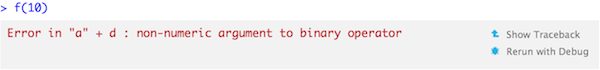
\includegraphics[width=4.35in]{screenshots/traceback-hidden.png}

Two options appear to the right of the error message: ``Show Traceback''
and ``Rerun with Debug''. If you click ``Show traceback'' you see:

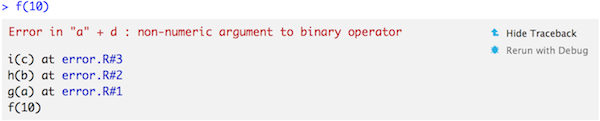
\includegraphics[width=4.35in]{screenshots/traceback-shown.png}

If you're not using Rstudio, you can use \texttt{traceback()} to get the
same information:

\begin{Shaded}
\begin{Highlighting}[]
\KeywordTok{traceback}\NormalTok{()}
\CommentTok{# 4: i(c) at exceptions-example.R#3}
\CommentTok{# 3: h(b) at exceptions-example.R#2}
\CommentTok{# 2: g(a) at exceptions-example.R#1}
\CommentTok{# 1: f(10)}
\end{Highlighting}
\end{Shaded}

Read the call stack from bottom to top: the initial call is
\texttt{f()}, which calls \texttt{g()}, then \texttt{h()}, then
\texttt{i()}, which triggers the error. If you're calling code that you
\texttt{source()}d into R, the traceback will also display the location
of the function, in the form \texttt{filename.r\#linenumber}. These are
clickable in Rstudio, and will take you to the corresponding line of
code in the editor.

Sometimes this is enough information to let you track down the error and
fix it. However, it's usually not. \texttt{traceback()} shows you where
the error occurred, but not why. The next useful tool is the interactive
debugger, which allows you to pause execution of a function and
interactively explore its state.

\subsection{Browsing on error}

The easiest way to enter the interactive debugger is through RStudio's
``Rerun with Debug'' tool. This reruns the command that created the
error, pausing execution where the error occurred. You're now in an
interactive state inside the function, and you can interact with any
object defined there. You'll see the corresponding code in the editor
(with the statement that will be run next highlighted), objects in the
current environment in the ``Environment'' pane, the call stack in a
``Traceback'' pane, and you can run arbitrary R code in the console.
\index{debugger, interactive}

As well as any regular R function, there are a few special commands you
can use in debug mode. You can access them either with the Rstudio
toolbar (
\includegraphics[width=2.48in]{screenshots/debug-toolbar.png})
or with the keyboard:

\begin{itemize}
\item
  Next, \texttt{n}: executes the next step in the function. Be careful
  if you have a variable named \texttt{n}; to print it you'll need to do
  \texttt{print(n)}.
\item
  Step into, 
\includegraphics[width=0.24in]{screenshots/step-into.png}
  or \texttt{s}: works like next, but if the next step is a function, it
  will step into that function so you can work through each line.
\item
  Finish, 
\includegraphics[width=0.24in]{screenshots/finish-loop.png} or
  \texttt{f}: finishes execution of the current loop or function.
\item
  Continue, \texttt{c}: leaves interactive debugging and continues
  regular execution of the function. This is useful if you've fixed the
  bad state and want to check that the function proceeds correctly.
\item
  Stop, \texttt{Q}: stops debugging, terminates the function, and
  returns to the global workspace. Use this once you've figured out
  where the problem is, and you're ready to fix it and reload the code.
\end{itemize}

There are two other slightly less useful commands that aren't available
in the toolbar:

\begin{itemize}
\item
  Enter: repeats the previous command. I find this too easy to activate
  accidentally, so I turn it off using
  \texttt{options(browserNLdisabled = TRUE)}.
\item
  \texttt{where}: prints stack trace of active calls (the interactive
  equivalent of \texttt{traceback}).
\end{itemize}

To enter this style of debugging outside of RStudio, you can use the
\texttt{error} option which specifies a function to run when an error
occurs. The function most similar to Rstudio's debug is
\texttt{browser()}: this will start an interactive console in the
environment where the error occurred. Use
\texttt{options(error = browser)} to turn it on, re-run the previous
command, then use \texttt{options(error = NULL)} to return to the
default error behaviour. You could automate this with the
\texttt{browseOnce()} function as defined below: \indexc{options(error)}

\begin{Shaded}
\begin{Highlighting}[]
\NormalTok{browseOnce <-}\StringTok{ }\NormalTok{function() \{}
  \NormalTok{old <-}\StringTok{ }\KeywordTok{getOption}\NormalTok{(}\StringTok{"error"}\NormalTok{)}
  \NormalTok{function() \{}
    \KeywordTok{options}\NormalTok{(}\DataTypeTok{error =} \NormalTok{old)}
    \KeywordTok{browser}\NormalTok{()}
  \NormalTok{\}}
\NormalTok{\}}
\KeywordTok{options}\NormalTok{(}\DataTypeTok{error =} \KeywordTok{browseOnce}\NormalTok{())}

\NormalTok{f <-}\StringTok{ }\NormalTok{function() }\KeywordTok{stop}\NormalTok{(}\StringTok{"!"}\NormalTok{)}
\CommentTok{# Enters browser}
\KeywordTok{f}\NormalTok{()}
\CommentTok{# Runs normally}
\KeywordTok{f}\NormalTok{()}
\end{Highlighting}
\end{Shaded}

(You'll learn more about functions that return functions in
\hyperref[functional-programming]{Functional programming}.)

There are two other useful functions that you can use with the
\texttt{error} option:

\begin{itemize}
\item
  \texttt{recover} is a step up from \texttt{browser}, as it allows you
  to enter the environment of any of the calls in the call stack. This
  is useful because often the root cause of the error is a number of
  calls back. \indexc{recover()}
\item
  \texttt{dump.frames} is an equivalent to \texttt{recover} for
  non-interactive code. It creates a \texttt{last.dump.rda} file in the
  current working directory. Then, in a later interactive R session, you
  load that file, and use \texttt{debugger()} to enter an interactive
  debugger with the same interface as \texttt{recover()}. This allows
  interactive debugging of batch code. \indexc{dump.frames()}

\begin{Shaded}
\begin{Highlighting}[]
\CommentTok{# In batch R process ----}
\NormalTok{dump_and_quit <-}\StringTok{ }\NormalTok{function() \{}
  \CommentTok{# Save debugging info to file last.dump.rda}
  \KeywordTok{dump.frames}\NormalTok{(}\DataTypeTok{to.file =} \OtherTok{TRUE}\NormalTok{)}
  \CommentTok{# Quit R with error status}
  \KeywordTok{q}\NormalTok{(}\DataTypeTok{status =} \DecValTok{1}\NormalTok{)}
\NormalTok{\}}
\KeywordTok{options}\NormalTok{(}\DataTypeTok{error =} \NormalTok{dump_and_quit)}

\CommentTok{# In a later interactive session ----}
\KeywordTok{load}\NormalTok{(}\StringTok{"last.dump.rda"}\NormalTok{)}
\KeywordTok{debugger}\NormalTok{()}
\end{Highlighting}
\end{Shaded}
\end{itemize}

To reset error behaviour to the default, use
\texttt{options(error = NULL)}. Then errors will print a message and
abort function execution.

\subsection{Browsing arbitrary code}

As well as entering an interactive console on error, you can enter it at
an arbitrary code location by using either an Rstudio breakpoint or
\texttt{browser()}. You can set a breakpoint in Rstudio by clicking to
the left of the line number, or pressing \texttt{Shift + F9}.
Equivalently, add \texttt{browser()} where you want execution to pause.
Breakpoints behave similarly to \texttt{browser()} but they are easier
to set (one click instead of nine key presses), and you don't run the
risk of accidentally including a \texttt{browser()} statement in your
source code. There are two small downsides to breakpoints:
\indexc{browser()} \index{breakpoints}

\begin{itemize}
\item
  There are a few unusual situations in which breakpoints will not work:
  read
  \href{http://www.rstudio.com/ide/docs/debugging/breakpoint-troubleshooting}{breakpoint
  troubleshooting} for more details.
\item
  RStudio currently does not support conditional breakpoints, whereas
  you can always put \texttt{browser()} inside an \texttt{if} statement.
\end{itemize}

As well as adding \texttt{browser()} yourself, there are two other
functions that will add it to code:

\begin{itemize}
\item
  \texttt{debug()} inserts a browser statement in the first line of the
  specified function. \texttt{undebug()} removes it. Alternatively, you
  can use \texttt{debugonce()} to browse only on the next run.
  \indexc{debug()}
\item
  \texttt{utils::setBreakpoint()} works similarly, but instead of taking
  a function name, it takes a file name and line number and finds the
  appropriate function for you. \indexc{setBreakpoint()}
\end{itemize}

These two functions are both special cases of \texttt{trace()}, which
inserts arbitrary code at any position in an existing function.
\texttt{trace()} is occasionally useful when you're debugging code that
you don't have the source for. To remove tracing from a function, use
\texttt{untrace()}. You can only perform one trace per function, but
that one trace can call multiple functions. \indexc{trace()}

\subsection{The call stack: \texttt{traceback()}, \texttt{where}, and
\texttt{recover()}}

Unfortunately the call stacks printed by \texttt{traceback()},
\texttt{browser()} + \texttt{where}, and \texttt{recover()} are not
consistent. The following table shows how the call stacks from a simple
nested set of calls are displayed by the three tools. \index{call stack}

\begin{longtable}[c]{@{}lll@{}}
\toprule\addlinespace
\texttt{traceback()} & \texttt{where} & \texttt{recover()}
\\\addlinespace
\midrule\endhead
\texttt{4: stop("Error")} & \texttt{where 1: stop("Error")} &
\texttt{1: f()}
\\\addlinespace
\texttt{3: h(x)} & \texttt{where 2: h(x)} & \texttt{2: g(x)}
\\\addlinespace
\texttt{2: g(x)} & \texttt{where 3: g(x)} & \texttt{3: h(x)}
\\\addlinespace
\texttt{1: f()} & \texttt{where 4: f()} &
\\\addlinespace
\bottomrule
\end{longtable}

Note that numbering is different between \texttt{traceback()} and
\texttt{where}, and that \texttt{recover()} displays calls in the
opposite order, and omits the call to \texttt{stop()}. RStudio displays
calls in the same order as \texttt{traceback()} but omits the numbers.

\subsection{Other types of failure}

There are other ways for a function to fail apart from throwing an error
or returning an incorrect result.

\begin{itemize}
\item
  A function may generate an unexpected warning. The easiest way to
  track down warnings is to convert them into errors with
  \texttt{options(warn = 2)} and use the regular debugging tools. When
  you do this you'll see some extra calls in the call stack, like
  \texttt{doWithOneRestart()}, \texttt{withOneRestart()},
  \texttt{withRestarts()}, and \texttt{.signalSimpleWarning()}. Ignore
  these: they are internal functions used to turn warnings into errors.
  \index{debugging!warnings}
\item
  A function may generate an unexpected message. There's no built-in
  tool to help solve this problem, but it's possible to create one:
  \index{debugging!messages}

\begin{Shaded}
\begin{Highlighting}[]
\NormalTok{message2error <-}\StringTok{ }\NormalTok{function(code) \{}
  \KeywordTok{withCallingHandlers}\NormalTok{(code, }\DataTypeTok{message =} \NormalTok{function(e) }\KeywordTok{stop}\NormalTok{(e))}
\NormalTok{\}}

\NormalTok{f <-}\StringTok{ }\NormalTok{function() }\KeywordTok{g}\NormalTok{()}
\NormalTok{g <-}\StringTok{ }\NormalTok{function() }\KeywordTok{message}\NormalTok{(}\StringTok{"Hi!"}\NormalTok{)}
\KeywordTok{g}\NormalTok{()}
\CommentTok{# Error in message("Hi!"): Hi!}
\KeywordTok{message2error}\NormalTok{(}\KeywordTok{g}\NormalTok{())}
\KeywordTok{traceback}\NormalTok{()}
\CommentTok{# 10: stop(e) at #2}
\CommentTok{# 9: (function (e) stop(e))(list(message = "Hi!\textbackslash{}n", }
\CommentTok{#      call = message("Hi!")))}
\CommentTok{# 8: signalCondition(cond)}
\CommentTok{# 7: doWithOneRestart(return(expr), restart)}
\CommentTok{# 6: withOneRestart(expr, restarts[[1L]])}
\CommentTok{# 5: withRestarts()}
\CommentTok{# 4: message("Hi!") at #1}
\CommentTok{# 3: g()}
\CommentTok{# 2: withCallingHandlers(code, message = function(e) stop(e)) }
\CommentTok{#      at #2}
\CommentTok{# 1: message2error(g())}
\end{Highlighting}
\end{Shaded}

  As with warnings, you'll need to ignore some of the calls on the
  traceback (i.e., the first two and the last seven).
\item
  A function might never return. This is particularly hard to debug
  automatically, but sometimes terminating the function and looking at
  the call stack is informative. Otherwise, use the basic debugging
  strategies described above.
\item
  The worst scenario is that your code might crash R completely, leaving
  you with no way to interactively debug your code. This indicates a bug
  in underlying C code. This is hard to debug. Sometimes an interactive
  debugger, like \texttt{gdb}, can be useful, but describing how to use
  it is beyond the scope of this book. \index{debugging!C code}

  If the crash is caused by base R code, post a reproducible example to
  R-help. If it's in a package, contact the package maintainer. If it's
  your own C or C++ code, you'll need to use numerous \texttt{print()}
  statements to narrow down the location of the bug, and then you'll
  need to use many more print statements to figure out which data
  structure doesn't have the properties that you expect.
\end{itemize}

\hyperdef{}{condition-handling}{\section{Condition
handling}\label{condition-handling}}

Unexpected errors require interactive debugging to figure out what went
wrong. Some errors, however, are expected, and you want to handle them
automatically. In R, expected errors crop up most frequently when you're
fitting many models to different datasets, such as bootstrap replicates.
Sometimes the model might fail to fit and throw an error, but you don't
want to stop everything. Instead, you want to fit as many models as
possible and then perform diagnostics after the fact. \index{conditions}

In R, there are three tools for handling conditions (including errors)
programmatically:

\begin{itemize}
\item
  \texttt{try()} gives you the ability to continue execution even when
  an error occurs.
\item
  \texttt{tryCatch()} lets you specify \textbf{handler} functions that
  control what happens when a condition is signalled.
\item
  \texttt{withCallingHandlers()} is a variant of \texttt{tryCatch()}
  that runs its handlers in a different context. It's rarely needed, but
  is useful to be aware of.
\end{itemize}

The following sections describe these tools in more detail.

\subsection{Ignore errors with try}\label{try}

\texttt{try()} allows execution to continue even after an error has
occurred. For example, normally if you run a function that throws an
error, it terminates immediately and doesn't return a value:
\indexc{try()}

\begin{Shaded}
\begin{Highlighting}[]
\NormalTok{f1 <-}\StringTok{ }\NormalTok{function(x) \{}
  \KeywordTok{log}\NormalTok{(x)}
  \DecValTok{10}
\NormalTok{\}}
\KeywordTok{f1}\NormalTok{(}\StringTok{"x"}\NormalTok{)}
\CommentTok{#> Error: non-numeric argument to mathematical function}
\end{Highlighting}
\end{Shaded}

However, if you wrap the statement that creates the error in
\texttt{try()}, the error message will be printed but execution will
continue:

\begin{Shaded}
\begin{Highlighting}[]
\NormalTok{f2 <-}\StringTok{ }\NormalTok{function(x) \{}
  \KeywordTok{try}\NormalTok{(}\KeywordTok{log}\NormalTok{(x))}
  \DecValTok{10}
\NormalTok{\}}
\KeywordTok{f2}\NormalTok{(}\StringTok{"a"}\NormalTok{)}
\CommentTok{#> Error in log(x) : non-numeric argument to mathematical function}
\CommentTok{#> [1] 10}
\end{Highlighting}
\end{Shaded}

You can suppress the message with \texttt{try(..., silent = TRUE)}.

To pass larger blocks of code to \texttt{try()}, wrap them in
\texttt{\{\}}:

\begin{Shaded}
\begin{Highlighting}[]
\KeywordTok{try}\NormalTok{(\{}
  \NormalTok{a <-}\StringTok{ }\DecValTok{1}
  \NormalTok{b <-}\StringTok{ "x"}
  \NormalTok{a +}\StringTok{ }\NormalTok{b}
\NormalTok{\})}
\end{Highlighting}
\end{Shaded}

You can also capture the output of the \texttt{try()} function. If
successful, it will be the last result evaluated in the block (just like
a function). If unsuccessful it will be an (invisible) object of class
``try-error'':

\begin{Shaded}
\begin{Highlighting}[]
\NormalTok{success <-}\StringTok{ }\KeywordTok{try}\NormalTok{(}\DecValTok{1} \NormalTok{+}\StringTok{ }\DecValTok{2}\NormalTok{)}
\NormalTok{failure <-}\StringTok{ }\KeywordTok{try}\NormalTok{(}\StringTok{"a"} \NormalTok{+}\StringTok{ "b"}\NormalTok{)}
\KeywordTok{class}\NormalTok{(success)}
\CommentTok{#> [1] "numeric"}
\KeywordTok{class}\NormalTok{(failure)}
\CommentTok{#> [1] "try-error"}
\end{Highlighting}
\end{Shaded}

\texttt{try()} is particularly useful when you're applying a function to
multiple elements in a list:

\begin{Shaded}
\begin{Highlighting}[]
\NormalTok{elements <-}\StringTok{ }\KeywordTok{list}\NormalTok{(}\DecValTok{1}\NormalTok{:}\DecValTok{10}\NormalTok{, }\KeywordTok{c}\NormalTok{(-}\DecValTok{1}\NormalTok{, }\DecValTok{10}\NormalTok{), }\KeywordTok{c}\NormalTok{(T, F), letters)}
\NormalTok{results <-}\StringTok{ }\KeywordTok{lapply}\NormalTok{(elements, log)}
\CommentTok{#> Warning: NaNs produced}
\CommentTok{#> Error: non-numeric argument to mathematical function}
\NormalTok{results <-}\StringTok{ }\KeywordTok{lapply}\NormalTok{(elements, function(x) }\KeywordTok{try}\NormalTok{(}\KeywordTok{log}\NormalTok{(x)))}
\CommentTok{#> Warning: NaNs produced}
\end{Highlighting}
\end{Shaded}

There isn't a built-in function to test for the try-error class, so
we'll define one. Then you can easily find the locations of errors with
\texttt{sapply()} (as discussed in \hyperref[functionals]{Functionals}),
and extract the successes or look at the inputs that lead to failures.

\begin{Shaded}
\begin{Highlighting}[]
\NormalTok{is.error <-}\StringTok{ }\NormalTok{function(x) }\KeywordTok{inherits}\NormalTok{(x, }\StringTok{"try-error"}\NormalTok{)}
\NormalTok{succeeded <-}\StringTok{ }\NormalTok{!}\KeywordTok{sapply}\NormalTok{(results, is.error)}

\CommentTok{# look at successful results}
\KeywordTok{str}\NormalTok{(results[succeeded])}
\CommentTok{#> List of 3}
\CommentTok{#>  $ : num [1:10] 0 0.693 1.099 1.386 1.609 ...}
\CommentTok{#>  $ : num [1:2] NaN 2.3}
\CommentTok{#>  $ : num [1:2] 0 -Inf}

\CommentTok{# look at inputs that failed}
\KeywordTok{str}\NormalTok{(elements[!succeeded])}
\CommentTok{#> List of 1}
\CommentTok{#>  $ : chr [1:26] "a" "b" "c" "d" ...}
\end{Highlighting}
\end{Shaded}

Another useful \texttt{try()} idiom is using a default value if an
expression fails. Simply assign the default value outside the try block,
and then run the risky code:

\begin{Shaded}
\begin{Highlighting}[]
\NormalTok{default <-}\StringTok{ }\OtherTok{NULL}
\KeywordTok{try}\NormalTok{(default <-}\StringTok{ }\KeywordTok{read.csv}\NormalTok{(}\StringTok{"possibly-bad-input.csv"}\NormalTok{), }\DataTypeTok{silent =} \OtherTok{TRUE}\NormalTok{)}
\end{Highlighting}
\end{Shaded}

There is also \texttt{plyr::failwith()}, which makes this strategy even
easier to implement. See \hyperref[output-fos]{Function Operators} for
more details.

\subsection{Handle conditions with \texttt{tryCatch()}}

\texttt{tryCatch()} is a general tool for handling conditions: in
addition to errors, you can take different actions for warnings,
messages, and interrupts. You've seen errors (made by \texttt{stop()}),
warnings (\texttt{warning()}) and messages (\texttt{message()}) before,
but interrupts are new. They can't be generated directly by the
programmer, but are raised when the user attempts to terminate execution
by pressing Ctrl + Break, Escape, or Ctrl + C (depending on the
platform). \indexc{tryCatch()} \index{errors!catching}

With \texttt{tryCatch()} you map conditions to \textbf{handlers}, named
functions that are called with the condition as an input. If a condition
is signalled, \texttt{tryCatch()} will call the first handler whose name
matches one of the classes of the condition. The only useful built-in
names are \texttt{error}, \texttt{warning}, \texttt{message},
\texttt{interrupt}, and the catch-all \texttt{condition}. A handler
function can do anything, but typically it will either return a value or
create a more informative error message. For example, the
\texttt{show\_condition()} function below sets up handlers that return
the type of condition signalled: \index{error handlers}

\begin{Shaded}
\begin{Highlighting}[]
\NormalTok{show_condition <-}\StringTok{ }\NormalTok{function(code) \{}
  \KeywordTok{tryCatch}\NormalTok{(code,}
    \DataTypeTok{error =} \NormalTok{function(c) }\StringTok{"error"}\NormalTok{,}
    \DataTypeTok{warning =} \NormalTok{function(c) }\StringTok{"warning"}\NormalTok{,}
    \DataTypeTok{message =} \NormalTok{function(c) }\StringTok{"message"}
  \NormalTok{)}
\NormalTok{\}}
\KeywordTok{show_condition}\NormalTok{(}\KeywordTok{stop}\NormalTok{(}\StringTok{"!"}\NormalTok{))}
\CommentTok{#> [1] "error"}
\KeywordTok{show_condition}\NormalTok{(}\KeywordTok{warning}\NormalTok{(}\StringTok{"?!"}\NormalTok{))}
\CommentTok{#> [1] "warning"}
\KeywordTok{show_condition}\NormalTok{(}\KeywordTok{message}\NormalTok{(}\StringTok{"?"}\NormalTok{))}
\CommentTok{#> [1] "message"}

\CommentTok{# If no condition is captured, tryCatch returns the }
\CommentTok{# value of the input}
\KeywordTok{show_condition}\NormalTok{(}\DecValTok{10}\NormalTok{)}
\CommentTok{#> [1] 10}
\end{Highlighting}
\end{Shaded}

You can use \texttt{tryCatch()} to implement \texttt{try()}. A simple
implementation is shown below. \texttt{base::try()} is more complicated
in order to make the error message look more like what you'd see if
\texttt{tryCatch()} wasn't used. Note the use of
\texttt{conditionMessage()} to extract the message associated with the
original error.

\begin{Shaded}
\begin{Highlighting}[]
\NormalTok{try2 <-}\StringTok{ }\NormalTok{function(code, }\DataTypeTok{silent =} \OtherTok{FALSE}\NormalTok{) \{}
  \KeywordTok{tryCatch}\NormalTok{(code, }\DataTypeTok{error =} \NormalTok{function(c) \{}
    \NormalTok{msg <-}\StringTok{ }\KeywordTok{conditionMessage}\NormalTok{(c)}
    \NormalTok{if (!silent) }\KeywordTok{message}\NormalTok{(c)}
    \KeywordTok{invisible}\NormalTok{(}\KeywordTok{structure}\NormalTok{(msg, }\DataTypeTok{class =} \StringTok{"try-error"}\NormalTok{))}
  \NormalTok{\})}
\NormalTok{\}}

\KeywordTok{try2}\NormalTok{(}\DecValTok{1}\NormalTok{)}
\CommentTok{#> [1] 1}
\KeywordTok{try2}\NormalTok{(}\KeywordTok{stop}\NormalTok{(}\StringTok{"Hi"}\NormalTok{))}
\KeywordTok{try2}\NormalTok{(}\KeywordTok{stop}\NormalTok{(}\StringTok{"Hi"}\NormalTok{), }\DataTypeTok{silent =} \OtherTok{TRUE}\NormalTok{)}
\end{Highlighting}
\end{Shaded}

As well as returning default values when a condition is signalled,
handlers can be used to make more informative error messages. For
example, by modifying the message stored in the error condition object,
the following function wraps \texttt{read.csv()} to add the file name to
any errors:

\begin{Shaded}
\begin{Highlighting}[]
\NormalTok{read.csv2 <-}\StringTok{ }\NormalTok{function(file, ...) \{}
  \KeywordTok{tryCatch}\NormalTok{(}\KeywordTok{read.csv}\NormalTok{(file, ...), }\DataTypeTok{error =} \NormalTok{function(c) \{}
    \NormalTok{c$message <-}\StringTok{ }\KeywordTok{paste0}\NormalTok{(c$message, }\StringTok{" (in "}\NormalTok{, file, }\StringTok{")"}\NormalTok{)}
    \KeywordTok{stop}\NormalTok{(c)}
  \NormalTok{\})}
\NormalTok{\}}
\KeywordTok{read.csv}\NormalTok{(}\StringTok{"code/dummy.csv"}\NormalTok{)}
\CommentTok{#> Error: cannot open the connection}
\KeywordTok{read.csv2}\NormalTok{(}\StringTok{"code/dummy.csv"}\NormalTok{)}
\CommentTok{#> Error: cannot open the connection (in code/dummy.csv)}
\end{Highlighting}
\end{Shaded}

Catching interrupts can be useful if you want to take special action
when the user tries to abort running code. But be careful, it's easy to
create a loop that you can never escape (unless you kill R)!
\index{interrupts}

\begin{Shaded}
\begin{Highlighting}[]
\CommentTok{# Don't let the user interrupt the code}
\NormalTok{i <-}\StringTok{ }\DecValTok{1}
\NormalTok{while(i <}\StringTok{ }\DecValTok{3}\NormalTok{) \{}
  \KeywordTok{tryCatch}\NormalTok{(\{}
    \KeywordTok{Sys.sleep}\NormalTok{(}\FloatTok{0.5}\NormalTok{)}
    \KeywordTok{message}\NormalTok{(}\StringTok{"Try to escape"}\NormalTok{)}
  \NormalTok{\}, }\DataTypeTok{interrupt =} \NormalTok{function(x) \{}
    \KeywordTok{message}\NormalTok{(}\StringTok{"Try again!"}\NormalTok{)}
    \NormalTok{i <<-}\StringTok{ }\NormalTok{i +}\StringTok{ }\DecValTok{1}
  \NormalTok{\})}
\NormalTok{\}}
\end{Highlighting}
\end{Shaded}

\texttt{tryCatch()} has one other argument: \texttt{finally}. It
specifies a block of code (not a function) to run regardless of whether
the initial expression succeeds or fails. This can be useful for clean
up (e.g., deleting files, closing connections). This is functionally
equivalent to using \texttt{on.exit()} but it can wrap smaller chunks of
code than an entire function. \indexc{on.exit()}

\subsection{\texttt{withCallingHandlers()}}

An alternative to \texttt{tryCatch()} is \texttt{withCallingHandlers()}.
There are two main differences between these functions:
\indexc{withCallingHandlers()}

\begin{itemize}
\item
  The return value of \texttt{tryCatch()} handlers is returned by
  \texttt{tryCatch()}, whereas the return value of
  \texttt{withCallingHandlers()} handlers is ignored:

\begin{Shaded}
\begin{Highlighting}[]
\NormalTok{f <-}\StringTok{ }\NormalTok{function() }\KeywordTok{stop}\NormalTok{(}\StringTok{"!"}\NormalTok{)}
\KeywordTok{tryCatch}\NormalTok{(}\KeywordTok{f}\NormalTok{(), }\DataTypeTok{error =} \NormalTok{function(e) }\DecValTok{1}\NormalTok{)}
\CommentTok{#> [1] 1}
\KeywordTok{withCallingHandlers}\NormalTok{(}\KeywordTok{f}\NormalTok{(), }\DataTypeTok{error =} \NormalTok{function(e) }\DecValTok{1}\NormalTok{)}
\CommentTok{#> Error: !}
\end{Highlighting}
\end{Shaded}
\item
  The handlers in \texttt{withCallingHandlers()} are called in the
  context of the call that generated the condition whereas the handlers
  in \texttt{tryCatch()} are called in the context of
  \texttt{tryCatch()}. This is shown here with \texttt{sys.calls()},
  which is the run-time equivalent of \texttt{traceback()} --- it lists
  all calls leading to the current function.

\begin{Shaded}
\begin{Highlighting}[]
\NormalTok{f <-}\StringTok{ }\NormalTok{function() }\KeywordTok{g}\NormalTok{()}
\NormalTok{g <-}\StringTok{ }\NormalTok{function() }\KeywordTok{h}\NormalTok{()}
\NormalTok{h <-}\StringTok{ }\NormalTok{function() }\KeywordTok{stop}\NormalTok{(}\StringTok{"!"}\NormalTok{)}

\KeywordTok{tryCatch}\NormalTok{(}\KeywordTok{f}\NormalTok{(), }\DataTypeTok{error =} \NormalTok{function(e) }\KeywordTok{print}\NormalTok{(}\KeywordTok{sys.calls}\NormalTok{()))}
\CommentTok{# [[1]] tryCatch(f(), error = function(e) print(sys.calls()))}
\CommentTok{# [[2]] tryCatchList(expr, classes, parentenv, handlers)}
\CommentTok{# [[3]] tryCatchOne(expr, names, parentenv, handlers[[1L]])}
\CommentTok{# [[4]] value[[3L]](cond)}

\KeywordTok{withCallingHandlers}\NormalTok{(}\KeywordTok{f}\NormalTok{(), }\DataTypeTok{error =} \NormalTok{function(e) }\KeywordTok{print}\NormalTok{(}\KeywordTok{sys.calls}\NormalTok{()))}
\CommentTok{# [[1]] withCallingHandlers(f(), }
\CommentTok{#    error = function(e) print(sys.calls()))}
\CommentTok{# [[2]] f()}
\CommentTok{# [[3]] g()}
\CommentTok{# [[4]] h()}
\CommentTok{# [[5]] stop("!")}
\CommentTok{# [[6]] .handleSimpleError(}
\CommentTok{#    function (e) print(sys.calls()), "!", quote(h()))}
\CommentTok{# [[7]] h(simpleError(msg, call))}
\end{Highlighting}
\end{Shaded}

  This also affects the order in which \texttt{on.exit()} is called.
\end{itemize}

These subtle differences are rarely useful, except when you're trying to
capture exactly what went wrong and pass it on to another function. For
most purposes, you should never need to use
\texttt{withCallingHandlers()}.

\subsection{Custom signal classes}

One of the challenges of error handling in R is that most functions just
call \texttt{stop()} with a string. That means if you want to figure out
if a particular error occurred, you have to look at the text of the
error message. This is error prone, not only because the text of the
error might change over time, but also because many error messages are
translated, so the message might be completely different to what you
expect. \index{errors!custom classes}

R has a little known and little used feature to solve this problem.
Conditions are S3 classes, so you can define your own classes if you
want to distinguish different types of error. Each condition signalling
function, \texttt{stop()}, \texttt{warning()}, and \texttt{message()},
can be given either a list of strings, or a custom S3 condition object.
Custom condition objects are not used very often, but are very useful
because they make it possible for the user to respond to different
errors in different ways. For example, ``expected'' errors (like a model
failing to converge for some input datasets) can be silently ignored,
while unexpected errors (like no disk space available) can be propagated
to the user.

R doesn't come with a built-in constructor function for conditions, but
we can easily add one. Conditions must contain \texttt{message} and
\texttt{call} components, and may contain other useful components. When
creating a new condition, it should always inherit from
\texttt{condition} and one of \texttt{error}, \texttt{warning}, or
\texttt{message}.

\begin{Shaded}
\begin{Highlighting}[]
\NormalTok{condition <-}\StringTok{ }\NormalTok{function(subclass, message, }\DataTypeTok{call =} \KeywordTok{sys.call}\NormalTok{(-}\DecValTok{1}\NormalTok{), ...) \{}
  \KeywordTok{structure}\NormalTok{(}
    \DataTypeTok{class =} \KeywordTok{c}\NormalTok{(subclass, }\StringTok{"condition"}\NormalTok{),}
    \KeywordTok{list}\NormalTok{(}\DataTypeTok{message =} \NormalTok{message, }\DataTypeTok{call =} \NormalTok{call),}
    \NormalTok{...}
  \NormalTok{)}
\NormalTok{\}}
\NormalTok{is.condition <-}\StringTok{ }\NormalTok{function(x) }\KeywordTok{inherits}\NormalTok{(x, }\StringTok{"condition"}\NormalTok{)}
\end{Highlighting}
\end{Shaded}

You can signal an arbitrary condition with \texttt{signalCondition()},
but nothing will happen unless you've instantiated a custom signal
handler (with \texttt{tryCatch()} or \texttt{withCallingHandlers()}).
Instead, use \texttt{stop()}, \texttt{warning()}, or \texttt{message()}
as appropriate to trigger the usual handling. R won't complain if the
class of your condition doesn't match the function, but you should avoid
this in real code. \indexc{stop()}

\begin{Shaded}
\begin{Highlighting}[]
\NormalTok{c <-}\StringTok{ }\KeywordTok{condition}\NormalTok{(}\KeywordTok{c}\NormalTok{(}\StringTok{"my_error"}\NormalTok{, }\StringTok{"error"}\NormalTok{), }\StringTok{"This is an error"}\NormalTok{)}
\KeywordTok{signalCondition}\NormalTok{(c)}
\CommentTok{# NULL}
\KeywordTok{stop}\NormalTok{(c)}
\CommentTok{# Error: This is an error}
\KeywordTok{warning}\NormalTok{(c)}
\CommentTok{# Warning message: This is an error}
\KeywordTok{message}\NormalTok{(c)}
\CommentTok{# This is an error}
\end{Highlighting}
\end{Shaded}

You can then use \texttt{tryCatch()} to take different actions for
different types of errors. In this example we make a convenient
\texttt{custom\_stop()} function that allows us to signal error
conditions with arbitrary classes. In a real application, it would be
better to have individual S3 constructor functions that you could
document, describing the error classes in more detail.

\begin{Shaded}
\begin{Highlighting}[]
\NormalTok{custom_stop <-}\StringTok{ }\NormalTok{function(subclass, message, }\DataTypeTok{call =} \KeywordTok{sys.call}\NormalTok{(-}\DecValTok{1}\NormalTok{), }
                        \NormalTok{...) \{}
  \NormalTok{c <-}\StringTok{ }\KeywordTok{condition}\NormalTok{(}\KeywordTok{c}\NormalTok{(subclass, }\StringTok{"error"}\NormalTok{), message, }\DataTypeTok{call =} \NormalTok{call, ...)}
  \KeywordTok{stop}\NormalTok{(c)}
\NormalTok{\}}

\NormalTok{my_log <-}\StringTok{ }\NormalTok{function(x) \{}
  \NormalTok{if (!}\KeywordTok{is.numeric}\NormalTok{(x))}
    \KeywordTok{custom_stop}\NormalTok{(}\StringTok{"invalid_class"}\NormalTok{, }\StringTok{"my_log() needs numeric input"}\NormalTok{)}
  \NormalTok{if (}\KeywordTok{any}\NormalTok{(x <}\StringTok{ }\DecValTok{0}\NormalTok{))}
    \KeywordTok{custom_stop}\NormalTok{(}\StringTok{"invalid_value"}\NormalTok{, }\StringTok{"my_log() needs positive inputs"}\NormalTok{)}

  \KeywordTok{log}\NormalTok{(x)}
\NormalTok{\}}
\KeywordTok{tryCatch}\NormalTok{(}
  \KeywordTok{my_log}\NormalTok{(}\StringTok{"a"}\NormalTok{),}
  \DataTypeTok{invalid_class =} \NormalTok{function(c) }\StringTok{"class"}\NormalTok{,}
  \DataTypeTok{invalid_value =} \NormalTok{function(c) }\StringTok{"value"}
\NormalTok{)}
\CommentTok{#> [1] "class"}
\end{Highlighting}
\end{Shaded}

Note that when using \texttt{tryCatch()} with multiple handlers and
custom classes, the first handler to match any class in the signal's
class hierarchy is called, not the best match. For this reason, you need
to make sure to put the most specific handlers first:

\begin{Shaded}
\begin{Highlighting}[]
\KeywordTok{tryCatch}\NormalTok{(}\KeywordTok{customStop}\NormalTok{(}\StringTok{"my_error"}\NormalTok{, }\StringTok{"!"}\NormalTok{),}
  \DataTypeTok{error =} \NormalTok{function(c) }\StringTok{"error"}\NormalTok{,}
  \DataTypeTok{my_error =} \NormalTok{function(c) }\StringTok{"my_error"}
\NormalTok{)}
\CommentTok{#> [1] "error"}
\KeywordTok{tryCatch}\NormalTok{(}\KeywordTok{custom_stop}\NormalTok{(}\StringTok{"my_error"}\NormalTok{, }\StringTok{"!"}\NormalTok{),}
  \DataTypeTok{my_error =} \NormalTok{function(c) }\StringTok{"my_error"}\NormalTok{,}
  \DataTypeTok{error =} \NormalTok{function(c) }\StringTok{"error"}
\NormalTok{)}
\CommentTok{#> [1] "my_error"}
\end{Highlighting}
\end{Shaded}

\subsection{Exercises}

\begin{itemize}
\item
  Compare the following two implementations of \texttt{message2error()}.
  What is the main advantage of \texttt{withCallingHandlers()} in this
  scenario? (Hint: look carefully at the traceback.)

\begin{Shaded}
\begin{Highlighting}[]
\NormalTok{message2error <-}\StringTok{ }\NormalTok{function(code) \{}
  \KeywordTok{withCallingHandlers}\NormalTok{(code, }\DataTypeTok{message =} \NormalTok{function(e) }\KeywordTok{stop}\NormalTok{(e))}
\NormalTok{\}}
\NormalTok{message2error <-}\StringTok{ }\NormalTok{function(code) \{}
  \KeywordTok{tryCatch}\NormalTok{(code, }\DataTypeTok{message =} \NormalTok{function(e) }\KeywordTok{stop}\NormalTok{(e))}
\NormalTok{\}}
\end{Highlighting}
\end{Shaded}
\end{itemize}

\hyperdef{}{defensive-programming}{\section{Defensive
programming}\label{defensive-programming}}

Defensive programming is the art of making code fail in a well-defined
manner even when something unexpected occurs. A key principle of
defensive programming is to ``fail fast'': as soon as something wrong is
discovered, signal an error. This is more work for author of the
function (you!), but it makes debugging easier for users because they
get errors early rather than later, after unexpected input has passed
through several functions. \index{defensive programming}
\index{fail fast}

In R, the ``fail fast'' principle is implemented in three ways:

\begin{itemize}
\item
  Be strict about what you accept. For example, if your function is not
  vectorised in its inputs, but uses functions that are, make sure to
  check that the inputs are scalars. You can use \texttt{stopifnot()},
  the \href{https://github.com/hadley/assertthat}{assertthat} package,
  or simple \texttt{if} statements and \texttt{stop()}.
\item
  Avoid functions that use non-standard evaluation, like
  \texttt{subset}, \texttt{transform}, and \texttt{with}. These
  functions save time when used interactively, but because they make
  assumptions to reduce typing, when they fail, they often fail with
  uninformative error messages. You can learn more about non-standard
  evaluation in \hyperref[nse]{non-standard evaluation}.
\item
  Avoid functions that return different types of output depending on
  their input. The two biggest offenders are \texttt{{[}} and
  \texttt{sapply()}. Whenever subsetting a data frame in a function, you
  should always use \texttt{drop = FALSE}, otherwise you will
  accidentally convert 1-column data frames into vectors. Similarly,
  never use \texttt{sapply()} inside a function: always use the stricter
  \texttt{vapply()} which will throw an error if the inputs are
  incorrect types and return the correct type of output even for
  zero-length inputs.
\end{itemize}

There is a tension between interactive analysis and programming. When
you're working interactively, you want R to do what you mean. If it
guesses wrong, you want to discover that right away so you can fix it.
When you're programming, you want functions that signal errors if
anything is even slightly wrong or underspecified. Keep this tension in
mind when writing functions. If you're writing functions to facilitate
interactive data analysis, feel free to guess what the analyst wants and
recover from minor misspecifications automatically. If you're writing
functions for programming, be strict. Never try to guess what the caller
wants.

\subsection{Exercises}

\begin{itemize}
\item
  The goal of the \texttt{col\_means()} function defined below is to
  compute the means of all numeric columns in a data frame.

\begin{Shaded}
\begin{Highlighting}[]
\NormalTok{col_means <-}\StringTok{ }\NormalTok{function(df) \{}
  \NormalTok{numeric <-}\StringTok{ }\KeywordTok{sapply}\NormalTok{(df, is.numeric)}
  \NormalTok{numeric_cols <-}\StringTok{ }\NormalTok{df[, numeric]}

  \KeywordTok{data.frame}\NormalTok{(}\KeywordTok{lapply}\NormalTok{(numeric_cols, mean))}
\NormalTok{\}}
\end{Highlighting}
\end{Shaded}

  However, the function is not robust to unusual inputs. Look at the
  following results, decide which ones are incorrect, and modify
  \texttt{col\_means()} to be more robust. (Hint: there are two function
  calls in \texttt{col\_means()} that are particularly prone to
  problems.)

\begin{Shaded}
\begin{Highlighting}[]
\KeywordTok{col_means}\NormalTok{(mtcars)}
\KeywordTok{col_means}\NormalTok{(mtcars[, }\DecValTok{0}\NormalTok{])}
\KeywordTok{col_means}\NormalTok{(mtcars[}\DecValTok{0}\NormalTok{, ])}
\KeywordTok{col_means}\NormalTok{(mtcars[, }\StringTok{"mpg"}\NormalTok{, }\DataTypeTok{drop =} \NormalTok{F])}
\KeywordTok{col_means}\NormalTok{(}\DecValTok{1}\NormalTok{:}\DecValTok{10}\NormalTok{)}
\KeywordTok{col_means}\NormalTok{(}\KeywordTok{as.matrix}\NormalTok{(mtcars))}
\KeywordTok{col_means}\NormalTok{(}\KeywordTok{as.list}\NormalTok{(mtcars))}

\NormalTok{mtcars2 <-}\StringTok{ }\NormalTok{mtcars}
\NormalTok{mtcars2[-}\DecValTok{1}\NormalTok{] <-}\StringTok{ }\KeywordTok{lapply}\NormalTok{(mtcars2[-}\DecValTok{1}\NormalTok{], as.character)}
\KeywordTok{col_means}\NormalTok{(mtcars2)}
\end{Highlighting}
\end{Shaded}
\item
  The following function ``lags'' a vector, returning a version of
  \texttt{x} that is \texttt{n} values behind the original. Improve the
  function so that it (1) returns a useful error message if \texttt{n}
  is not a vector, and (2) has reasonable behaviour when \texttt{n} is 0
  or longer than \texttt{x}.

\begin{Shaded}
\begin{Highlighting}[]
\NormalTok{lag <-}\StringTok{ }\NormalTok{function(x, }\DataTypeTok{n =} \NormalTok{1L) \{}
  \NormalTok{xlen <-}\StringTok{ }\KeywordTok{length}\NormalTok{(x)}
  \KeywordTok{c}\NormalTok{(}\KeywordTok{rep}\NormalTok{(}\OtherTok{NA}\NormalTok{, n), x[}\KeywordTok{seq_len}\NormalTok{(xlen -}\StringTok{ }\NormalTok{n)])}
\NormalTok{\}}
\end{Highlighting}
\end{Shaded}
\end{itemize}

\hyperdef{}{debugging-answers}{\section{Quiz
answers}\label{debugging-answers}}

\begin{enumerate}
\def\labelenumi{\arabic{enumi}.}
\item
  The most useful tool to determine where a error occured is
  \texttt{traceback()}. Or use Rstudio, which displays it automatically
  where an error occurs.
\item
  \texttt{browser()} pauses execution at the specified line and allows
  you to enter an interactive environment. In that environment, there
  are five useful commands: \texttt{n}, execute the next command;
  \texttt{s}, step into the next function; \texttt{f}, finish the
  current loop or function; \texttt{c}, continue execution normally;
  \texttt{Q}, stop the function and return to the console.
\item
  You could use \texttt{try()} or \texttt{tryCatch()}.
\item
  Because you can then capture specific types of error with
  \texttt{tryCatch()}, rather than relying on the comparison of error
  strings, which is risky, especially when messages are translated.
\end{enumerate}


\part{Functional programming}
\chapter{Functional programming}\label{functional-programming}

R, at its heart, is a functional programming (FP) language. This means
that it provides many tools for the creation and manipulation of
functions. In particular, R has what's known as first class functions.
You can do anything with functions that you can do with vectors: you can
assign them to variables, store them in lists, pass them as arguments to
other functions, create them inside functions, and even return them as
the result of a function. \index{functional programming}

The chapter starts by showing a motivating example, removing redundancy
and duplication in code used to clean and summarise data. Then you'll
learn about the three building blocks of functional programming:
anonymous functions, closures (functions written by functions), and
lists of functions. These pieces are twined together in the conclusion
which shows how to build a suite of tools for numerical integration,
starting from very simple primitives. This is a recurring theme in FP:
start with small, easy-to-understand building blocks, combine them into
more complex structures, and apply them with confidence.

The discussion of functional programming continues in the following two
chapters: \hyperref[functionals]{functionals} explores functions that
take functions as arguments and return vectors as output, and
\hyperref[function-operators]{function operators} explores functions
that take functions as input and return them as output.

\paragraph{Outline}

\begin{itemize}
\item
  \hyperref[fp-motivation]{Motivation} motivates functional programming
  using a common problem: cleaning and summarising data before serious
  analysis.
\item
  \hyperref[anonymous-functions]{Anonymous functions} shows you a side
  of functions that you might not have known about: you can use
  functions without giving them a name.
\item
  \hyperref[closures]{Closures} introduces the closure, a function
  written by another function. A closure can access its own arguments,
  and variables defined in its parent.
\item
  \hyperref[lists-of-functions]{Lists of functions} shows how to put
  functions in a list, and explains why you might care.
\item
  \hyperref[numerical-integration]{Numerical integration} concludes the
  chapter with a case study that uses anonymous functions, closures and
  lists of functions to build a flexible toolkit for numerical
  integration.
\end{itemize}

\paragraph{Prequisites}

You should be familiar with the basic rules of lexical scoping, as
described in \hyperref[lexical-scoping]{lexical scoping}. Make sure
you've installed the pryr package with \texttt{install.packages("pryr")}

\hyperdef{}{fp-motivation}{\section{Motivation}\label{fp-motivation}}

Imagine you've loaded a data file, like the one below, that uses \(-99\)
to represent missing values. You want to replace all the \(-99\)s with
\texttt{NA}s.

\begin{Shaded}
\begin{Highlighting}[]
\CommentTok{# Generate a sample dataset}
\KeywordTok{set.seed}\NormalTok{(}\DecValTok{1014}\NormalTok{)}
\NormalTok{df <-}\StringTok{ }\KeywordTok{data.frame}\NormalTok{(}\KeywordTok{replicate}\NormalTok{(}\DecValTok{6}\NormalTok{, }\KeywordTok{sample}\NormalTok{(}\KeywordTok{c}\NormalTok{(}\DecValTok{1}\NormalTok{:}\DecValTok{10}\NormalTok{, -}\DecValTok{99}\NormalTok{), }\DecValTok{6}\NormalTok{, }\DataTypeTok{rep =} \OtherTok{TRUE}\NormalTok{)))}
\KeywordTok{names}\NormalTok{(df) <-}\StringTok{ }\NormalTok{letters[}\DecValTok{1}\NormalTok{:}\DecValTok{6}\NormalTok{]}
\NormalTok{df}
\CommentTok{#>    a  b c   d   e f}
\CommentTok{#> 1  1  6 1   5 -99 1}
\CommentTok{#> 2 10  4 4 -99   9 3}
\CommentTok{#> 3  7  9 5   4   1 4}
\CommentTok{#> 4  2  9 3   8   6 8}
\CommentTok{#> 5  1 10 5   9   8 6}
\CommentTok{#> 6  6  2 1   3   8 5}
\end{Highlighting}
\end{Shaded}

When you first started writing R code, you might have solved the problem
with copy-and-paste:

\begin{Shaded}
\begin{Highlighting}[]
\NormalTok{df$a[df$a ==}\StringTok{ }\NormalTok{-}\DecValTok{99}\NormalTok{] <-}\StringTok{ }\OtherTok{NA}
\NormalTok{df$b[df$b ==}\StringTok{ }\NormalTok{-}\DecValTok{99}\NormalTok{] <-}\StringTok{ }\OtherTok{NA}
\NormalTok{df$c[df$c ==}\StringTok{ }\NormalTok{-}\DecValTok{98}\NormalTok{] <-}\StringTok{ }\OtherTok{NA}
\NormalTok{df$d[df$d ==}\StringTok{ }\NormalTok{-}\DecValTok{99}\NormalTok{] <-}\StringTok{ }\OtherTok{NA}
\NormalTok{df$e[df$e ==}\StringTok{ }\NormalTok{-}\DecValTok{99}\NormalTok{] <-}\StringTok{ }\OtherTok{NA}
\NormalTok{df$f[df$g ==}\StringTok{ }\NormalTok{-}\DecValTok{99}\NormalTok{] <-}\StringTok{ }\OtherTok{NA}
\end{Highlighting}
\end{Shaded}

One problem with copy-and-paste is that it's easy to make mistakes. Can
you spot the two in the block above? These mistakes are inconsistencies
that arose because we didn't have an authorative description of the
desired action (replace \(-99\) with \texttt{NA}). Duplicating an action
makes bugs more likely and makes it harder to change code. For example,
if the code for a missing value changes from \(-99\) to 9999, you'd need
to make the change in multiple places.

To prevent bugs and to make more flexible code, adopt the ``do not
repeat yourself'', or DRY, principle. Popularised by the
\href{http://pragprog.com/about}{``pragmatic programmers''}, Dave Thomas
and Andy Hunt, this principle states: ``every piece of knowledge must
have a single, unambiguous, authoritative representation within a
system''. FP tools are valuable because they provide tools to reduce
duplication.

We can start applying FP ideas by writing a function that fixes the
missing values in a single vector:

\begin{Shaded}
\begin{Highlighting}[]
\NormalTok{fix_missing <-}\StringTok{ }\NormalTok{function(x) \{}
  \NormalTok{x[x ==}\StringTok{ }\NormalTok{-}\DecValTok{99}\NormalTok{] <-}\StringTok{ }\OtherTok{NA}
  \NormalTok{x}
\NormalTok{\}}
\NormalTok{df$a <-}\StringTok{ }\KeywordTok{fix_missing}\NormalTok{(df$a)}
\NormalTok{df$b <-}\StringTok{ }\KeywordTok{fix_missing}\NormalTok{(df$b)}
\NormalTok{df$c <-}\StringTok{ }\KeywordTok{fix_missing}\NormalTok{(df$c)}
\NormalTok{df$d <-}\StringTok{ }\KeywordTok{fix_missing}\NormalTok{(df$d)}
\NormalTok{df$e <-}\StringTok{ }\KeywordTok{fix_missing}\NormalTok{(df$e)}
\NormalTok{df$f <-}\StringTok{ }\KeywordTok{fix_missing}\NormalTok{(df$e)}
\end{Highlighting}
\end{Shaded}

This reduces the scope of possible mistakes, but it doesn't eliminate
them: you can no longer accidentally type -98 instead of -99, but you
can still mess up the name of variable. The next step is to remove this
possible source of error by combining two functions. One function,
\texttt{fix\_missing()}, knows how to fix a single vector; the other,
\texttt{lapply()}, knows how to do something to each column in a data
frame.

\texttt{lapply()} takes three inputs: \texttt{x}, a list; \texttt{f}, a
function; and \texttt{...}, other arguments to pass to \texttt{f()}. It
applies the function to each element of the list and returns a new list.
\texttt{lapply(x, f, ...)} is equivalent to the following for loop:

\begin{Shaded}
\begin{Highlighting}[]
\NormalTok{out <-}\StringTok{ }\KeywordTok{vector}\NormalTok{(}\StringTok{"list"}\NormalTok{, }\KeywordTok{length}\NormalTok{(x))}
\NormalTok{for (i in }\KeywordTok{seq_along}\NormalTok{(x)) \{}
  \NormalTok{out[[i]] <-}\StringTok{ }\KeywordTok{f}\NormalTok{(x[[i]], ...)}
\NormalTok{\}}
\end{Highlighting}
\end{Shaded}

The real \texttt{lapply()} is rather more complicated since it's
implemented in C for efficiency, but the essence of the algorithm is the
same. \texttt{lapply()} is called a \textbf{functional}, because it
takes a function as an argument. Functionals are an important part of
functional programming. You'll learn more about them in
\hyperref[functionals]{functionals}.

We can apply \texttt{lapply()} to this problem because data frames are
lists. We just need a neat little trick to make sure we get back a data
frame, not a list. Instead of assigning the results of \texttt{lapply()}
to \texttt{df}, we'll assign them to \texttt{df{[}{]}}. R's usual rules
ensure that we get a data frame, not a list. (If this comes as a
surprise, you might want to read \hyperref[subassignment]{subsetting and
assignment}.) Putting these pieces together gives us:

\begin{Shaded}
\begin{Highlighting}[]
\NormalTok{fix_missing <-}\StringTok{ }\NormalTok{function(x) \{}
  \NormalTok{x[x ==}\StringTok{ }\NormalTok{-}\DecValTok{99}\NormalTok{] <-}\StringTok{ }\OtherTok{NA}
  \NormalTok{x}
\NormalTok{\}}
\NormalTok{df[] <-}\StringTok{ }\KeywordTok{lapply}\NormalTok{(df, fix_missing)}
\end{Highlighting}
\end{Shaded}

This code has five advantages over copy and paste:

\begin{itemize}
\item
  It's more compact.
\item
  If the code for a missing value changes, it only needs to be updated
  in one place.
\item
  It works for any number of columns. There is no way to accidentally
  miss a column.
\item
  There is no way to accidentally treat one column differently than
  another.
\item
  It is easy to generalise this technique to a subset of columns:

\begin{Shaded}
\begin{Highlighting}[]
\NormalTok{df[}\DecValTok{1}\NormalTok{:}\DecValTok{5}\NormalTok{] <-}\StringTok{ }\KeywordTok{lapply}\NormalTok{(df[}\DecValTok{1}\NormalTok{:}\DecValTok{5}\NormalTok{], fix_missing)}
\end{Highlighting}
\end{Shaded}
\end{itemize}

The key idea is function composition. Take two simple functions, one
which does something to every column and one which fixes missing values,
and combine them to fix missing values in every column. Writing simple
functions that can be understood in isolation and then composed is a
powerful technique.

What if different columns used different codes for missing values? You
might be tempted to copy-and-paste:

\begin{Shaded}
\begin{Highlighting}[]
\NormalTok{fix_missing_99 <-}\StringTok{ }\NormalTok{function(x) \{}
  \NormalTok{x[x ==}\StringTok{ }\NormalTok{-}\DecValTok{99}\NormalTok{] <-}\StringTok{ }\OtherTok{NA}
  \NormalTok{x}
\NormalTok{\}}
\NormalTok{fix_missing_999 <-}\StringTok{ }\NormalTok{function(x) \{}
  \NormalTok{x[x ==}\StringTok{ }\NormalTok{-}\DecValTok{999}\NormalTok{] <-}\StringTok{ }\OtherTok{NA}
  \NormalTok{x}
\NormalTok{\}}
\NormalTok{fix_missing_9999 <-}\StringTok{ }\NormalTok{function(x) \{}
  \NormalTok{x[x ==}\StringTok{ }\NormalTok{-}\DecValTok{999}\NormalTok{] <-}\StringTok{ }\OtherTok{NA}
  \NormalTok{x}
\NormalTok{\}}
\end{Highlighting}
\end{Shaded}

As before, it's easy to create bugs. Instead we could use closures,
functions that make and return functions. Closures allow us to make
functions based on a template:

\begin{Shaded}
\begin{Highlighting}[]
\NormalTok{missing_fixer <-}\StringTok{ }\NormalTok{function(na_value) \{}
  \NormalTok{function(x) \{}
    \NormalTok{x[x ==}\StringTok{ }\NormalTok{na_value] <-}\StringTok{ }\OtherTok{NA}
    \NormalTok{x}
  \NormalTok{\}}
\NormalTok{\}}
\NormalTok{fix_missing_99 <-}\StringTok{ }\KeywordTok{missing_fixer}\NormalTok{(-}\DecValTok{99}\NormalTok{)}
\NormalTok{fix_missing_999 <-}\StringTok{ }\KeywordTok{missing_fixer}\NormalTok{(-}\DecValTok{999}\NormalTok{)}

\KeywordTok{fix_missing_99}\NormalTok{(}\KeywordTok{c}\NormalTok{(-}\DecValTok{99}\NormalTok{, -}\DecValTok{999}\NormalTok{))}
\CommentTok{#> [1]   NA -999}
\KeywordTok{fix_missing_999}\NormalTok{(}\KeywordTok{c}\NormalTok{(-}\DecValTok{99}\NormalTok{, -}\DecValTok{999}\NormalTok{))}
\CommentTok{#> [1] -99  NA}
\end{Highlighting}
\end{Shaded}

\begin{shortbox}\Boxhead{Extra argument}

In this case, you could argue that we should just add another argument:

\begin{Shaded}
\begin{Highlighting}[]
\NormalTok{fix_missing <-}\StringTok{ }\NormalTok{function(x, na.value) \{}
  \NormalTok{x[x ==}\StringTok{ }\NormalTok{na.value] <-}\StringTok{ }\OtherTok{NA}
  \NormalTok{x}
\NormalTok{\}}
\end{Highlighting}
\end{Shaded}

That's a reasonable solution here, but it doesn't always work well in
every situation. We'll see more compelling uses for closures in
\hyperref[functionals-math]{MLE}.

\end{shortbox}

Now consider a related problem. Once you've cleaned up your data, you
might want to compute the same set of numerical summaries for each
variable. You could write code like this:

\begin{Shaded}
\begin{Highlighting}[]
\KeywordTok{mean}\NormalTok{(df$a)}
\KeywordTok{median}\NormalTok{(df$a)}
\KeywordTok{sd}\NormalTok{(df$a)}
\KeywordTok{mad}\NormalTok{(df$a)}
\KeywordTok{IQR}\NormalTok{(df$a)}

\KeywordTok{mean}\NormalTok{(df$b)}
\KeywordTok{median}\NormalTok{(df$b)}
\KeywordTok{sd}\NormalTok{(df$b)}
\KeywordTok{mad}\NormalTok{(df$b)}
\KeywordTok{IQR}\NormalTok{(df$b)}
\end{Highlighting}
\end{Shaded}

But again, you'd be better off identifying and removing duplicate items.
Take a minute or two to think about how you might tackle this problem
before reading on.

One approach would be to write a summary function and then apply it to
each column:

\begin{Shaded}
\begin{Highlighting}[]
\NormalTok{summary <-}\StringTok{ }\NormalTok{function(x) \{}
  \KeywordTok{c}\NormalTok{(}\KeywordTok{mean}\NormalTok{(x), }\KeywordTok{median}\NormalTok{(x), }\KeywordTok{sd}\NormalTok{(x), }\KeywordTok{mad}\NormalTok{(x), }\KeywordTok{IQR}\NormalTok{(x))}
\NormalTok{\}}
\KeywordTok{lapply}\NormalTok{(df, summary)}
\end{Highlighting}
\end{Shaded}

That's a great start, but there's still some duplication. It's easier to
see if we make the summary function more realistic:

\begin{Shaded}
\begin{Highlighting}[]
\NormalTok{summary <-}\StringTok{ }\NormalTok{function(x) \{}
 \KeywordTok{c}\NormalTok{(}\KeywordTok{mean}\NormalTok{(x, }\DataTypeTok{na.rm =} \OtherTok{TRUE}\NormalTok{),}
   \KeywordTok{median}\NormalTok{(x, }\DataTypeTok{na.rm =} \OtherTok{TRUE}\NormalTok{),}
   \KeywordTok{sd}\NormalTok{(x, }\DataTypeTok{na.rm =} \OtherTok{TRUE}\NormalTok{),}
   \KeywordTok{mad}\NormalTok{(x, }\DataTypeTok{na.rm =} \OtherTok{TRUE}\NormalTok{),}
   \KeywordTok{IQR}\NormalTok{(x, }\DataTypeTok{na.rm =} \OtherTok{TRUE}\NormalTok{))}
\NormalTok{\}}
\end{Highlighting}
\end{Shaded}

All five functions are called with the same arguments (\texttt{x} and
\texttt{na.rm}) repeated five times. As always, duplication makes our
code fragile: it's easier to introduce bugs and harder to adapt to
changing requirements.

To remove this source of duplication, you can take advantage of another
functional programming technique: storing functions in lists.

\begin{Shaded}
\begin{Highlighting}[]
\NormalTok{summary <-}\StringTok{ }\NormalTok{function(x) \{}
  \NormalTok{funs <-}\StringTok{ }\KeywordTok{c}\NormalTok{(mean, median, sd, mad, IQR)}
  \KeywordTok{lapply}\NormalTok{(funs, function(f) }\KeywordTok{f}\NormalTok{(x, }\DataTypeTok{na.rm =} \OtherTok{TRUE}\NormalTok{))}
\NormalTok{\}}
\end{Highlighting}
\end{Shaded}

This chapter discusses these techniques in more detail. But before you
can start learning them, you need to learn the simplest FP tool, the
anonymous function.

\hyperdef{}{anonymous-functions}{\section{Anonymous
functions}\label{anonymous-functions}}

In R, functions are objects in their own right. They aren't
automatically bound to a name. Unlike many languages (e.g., C, C++,
Python, and Ruby), R doesn't have a special syntax for creating a named
function: when you create a function, you use the regular assignment
operator to give it a name. If you choose not to give the function a
name, you get an \textbf{anonymous function}.
\index{functions!anonymous} \index{anoynmous functions}

You use an anonymous function when it's not worth the effort to give it
a name:

\begin{Shaded}
\begin{Highlighting}[]
\KeywordTok{lapply}\NormalTok{(mtcars, function(x) }\KeywordTok{length}\NormalTok{(}\KeywordTok{unique}\NormalTok{(x)))}
\KeywordTok{Filter}\NormalTok{(function(x) !}\KeywordTok{is.numeric}\NormalTok{(x), mtcars)}
\KeywordTok{integrate}\NormalTok{(function(x) }\KeywordTok{sin}\NormalTok{(x) ^}\StringTok{ }\DecValTok{2}\NormalTok{, }\DecValTok{0}\NormalTok{, pi)}
\end{Highlighting}
\end{Shaded}

Like all functions in R, anonymous functions have \texttt{formals()}, a
\texttt{body()}, and a parent \texttt{environment()}:

\begin{Shaded}
\begin{Highlighting}[]
\KeywordTok{formals}\NormalTok{(function(}\DataTypeTok{x =} \DecValTok{4}\NormalTok{) }\KeywordTok{g}\NormalTok{(x) +}\StringTok{ }\KeywordTok{h}\NormalTok{(x))}
\CommentTok{#> $x}
\CommentTok{#> [1] 4}
\KeywordTok{body}\NormalTok{(function(}\DataTypeTok{x =} \DecValTok{4}\NormalTok{) }\KeywordTok{g}\NormalTok{(x) +}\StringTok{ }\KeywordTok{h}\NormalTok{(x))}
\CommentTok{#> g(x) + h(x)}
\KeywordTok{environment}\NormalTok{(function(}\DataTypeTok{x =} \DecValTok{4}\NormalTok{) }\KeywordTok{g}\NormalTok{(x) +}\StringTok{ }\KeywordTok{h}\NormalTok{(x))}
\CommentTok{#> <environment: R_GlobalEnv>}
\end{Highlighting}
\end{Shaded}

You can call an anonymous function without giving it a name, but the
code is a little tricky to read because you must use parentheses in two
different ways: first, to call a function, and second to make it clear
that you want to call the anonymous function itself, as opposed to
calling a (possibly invalid) function \emph{inside} the anonymous
function:

\begin{Shaded}
\begin{Highlighting}[]
\CommentTok{# This does not call the anonymous function.}
\CommentTok{# (Note that "3" is not a valid function.)}
\NormalTok{function(x) }\DecValTok{3}\NormalTok{()}
\CommentTok{#> function(x) 3()}

\CommentTok{# With appropriate parenthesis, the function is called:}
\NormalTok{(function(x) }\DecValTok{3}\NormalTok{)()}
\CommentTok{#> [1] 3}

\CommentTok{# So this anonymous function syntax}
\NormalTok{(function(x) x +}\StringTok{ }\DecValTok{3}\NormalTok{)(}\DecValTok{10}\NormalTok{)}
\CommentTok{#> [1] 13}

\CommentTok{# behaves exactly the same as}
\NormalTok{f <-}\StringTok{ }\NormalTok{function(x) x +}\StringTok{ }\DecValTok{3}
\KeywordTok{f}\NormalTok{(}\DecValTok{10}\NormalTok{)}
\CommentTok{#> [1] 13}
\end{Highlighting}
\end{Shaded}

You can call anonymous functions with named arguments, but doing so is a
good sign that your function needs a name.

One of the most common uses for anonymous functions is to create
closures, functions made by other functions. Closures are described in
the next section.

\subsection{Exercises}

\begin{enumerate}
\def\labelenumi{\arabic{enumi}.}
\item
  Given a function, like \texttt{"mean"}, \texttt{match.fun()} lets you
  find a function. Given a function, can you find its name? Why doesn't
  that make sense in R?
\item
  Use \texttt{lapply()} and an anonymous function to find the
  coefficient of variation (the standard deviation divided by the mean)
  for all columns in the \texttt{mtcars} dataset.
\item
  Use \texttt{integrate()} and an anonymous function to find the area
  under the curve for the following functions. Use
  \href{http://www.wolframalpha.com/}{Wolfram Alpha} to check your
  answers.

  \begin{enumerate}
  \def\labelenumii{\arabic{enumii}.}
  \itemsep1pt\parskip0pt\parsep0pt
  \item
    \texttt{y = x \^{} 2 - x}, x in {[}0, 10{]}
  \item
    \texttt{y = sin(x) + cos(x)}, x in {[}-\(\pi\), \(\pi\){]}
  \item
    \texttt{y = exp(x) / x}, x in {[}10, 20{]}
  \end{enumerate}
\item
  A good rule of thumb is that an anonymous function should fit on one
  line and shouldn't need to use \texttt{\{\}}. Review your code. Where
  could you have used an anonymous function instead of a named function?
  Where should you have used a named function instead of an anonymous
  function?
\end{enumerate}

\hyperdef{}{closures}{\section{Closures}\label{closures}}

\begin{quote}
``An object is data with functions. A closure is a function with data.''
--- John D. Cook
\end{quote}

One use of anonymous functions is to create small functions that are not
worth naming. Another important use is to create closures, functions
written by functions. Closures get their name because they
\textbf{enclose} the environment of the parent function and can access
all its variables. This is useful because it allows us to have two
levels of parameters: a parent level that controls operation and a child
level that does the work. \index{closures}
\index{functions!closures|see{closures}}

The following example uses this idea to generate a family of power
functions in which a parent function (\texttt{power()}) creates two
child functions (\texttt{square()} and \texttt{cube()}).

\begin{Shaded}
\begin{Highlighting}[]
\NormalTok{power <-}\StringTok{ }\NormalTok{function(exponent) \{}
  \NormalTok{function(x) \{}
    \NormalTok{x ^}\StringTok{ }\NormalTok{exponent}
  \NormalTok{\}}
\NormalTok{\}}

\NormalTok{square <-}\StringTok{ }\KeywordTok{power}\NormalTok{(}\DecValTok{2}\NormalTok{)}
\KeywordTok{square}\NormalTok{(}\DecValTok{2}\NormalTok{)}
\CommentTok{#> [1] 4}
\KeywordTok{square}\NormalTok{(}\DecValTok{4}\NormalTok{)}
\CommentTok{#> [1] 16}

\NormalTok{cube <-}\StringTok{ }\KeywordTok{power}\NormalTok{(}\DecValTok{3}\NormalTok{)}
\KeywordTok{cube}\NormalTok{(}\DecValTok{2}\NormalTok{)}
\CommentTok{#> [1] 8}
\KeywordTok{cube}\NormalTok{(}\DecValTok{4}\NormalTok{)}
\CommentTok{#> [1] 64}
\end{Highlighting}
\end{Shaded}

When you print a closure, you don't see anything terribly useful:

\begin{Shaded}
\begin{Highlighting}[]
\NormalTok{square}
\CommentTok{#> function(x) \{}
\CommentTok{#>     x ^ exponent}
\CommentTok{#>   \}}
\CommentTok{#> <environment: 0x7fda09128f20>}
\NormalTok{cube}
\CommentTok{#> function(x) \{}
\CommentTok{#>     x ^ exponent}
\CommentTok{#>   \}}
\CommentTok{#> <environment: 0x7fda04748a60>}
\end{Highlighting}
\end{Shaded}

That's because the function itself doesn't change. The difference is the
enclosing environment, \texttt{environment(square)}. One way to see the
contents of the environment is to convert it to a list:
\index{environments!of a closure}

\begin{Shaded}
\begin{Highlighting}[]
\KeywordTok{as.list}\NormalTok{(}\KeywordTok{environment}\NormalTok{(square))}
\CommentTok{#> $exponent}
\CommentTok{#> [1] 2}
\KeywordTok{as.list}\NormalTok{(}\KeywordTok{environment}\NormalTok{(cube))}
\CommentTok{#> $exponent}
\CommentTok{#> [1] 3}
\end{Highlighting}
\end{Shaded}

Another way to see what's going on is to use \texttt{pryr::unenclose()}.
This function replaces variables defined in the enclosing environment
with their values:

\begin{Shaded}
\begin{Highlighting}[]
\KeywordTok{library}\NormalTok{(pryr)}
\KeywordTok{unenclose}\NormalTok{(square)}
\CommentTok{#> function (x) }
\CommentTok{#> \{}
\CommentTok{#>     x^2}
\CommentTok{#> \}}
\KeywordTok{unenclose}\NormalTok{(cube)}
\CommentTok{#> function (x) }
\CommentTok{#> \{}
\CommentTok{#>     x^3}
\CommentTok{#> \}}
\end{Highlighting}
\end{Shaded}

The parent environment of a closure is the execution environment of the
function that created it, as shown by this code:

\begin{Shaded}
\begin{Highlighting}[]
\NormalTok{power <-}\StringTok{ }\NormalTok{function(exponent) \{}
  \KeywordTok{print}\NormalTok{(}\KeywordTok{environment}\NormalTok{())}
  \NormalTok{function(x) x ^}\StringTok{ }\NormalTok{exponent}
\NormalTok{\}}
\NormalTok{zero <-}\StringTok{ }\KeywordTok{power}\NormalTok{(}\DecValTok{0}\NormalTok{)}
\CommentTok{#> <environment: 0x7fda04cc0b18>}
\KeywordTok{environment}\NormalTok{(zero)}
\CommentTok{#> <environment: 0x7fda04cc0b18>}
\end{Highlighting}
\end{Shaded}

The execution environment normally disappears after the function returns
a value. However, functions capture their enclosing environments. This
means when function a returns function b, function b captures and stores
the execution environment of function a, and it doesn't disappear. (This
has important consequences for memory use, see \hyperref[gc]{memory
usage} for details.)

In R, almost every function is a closure. All functions remember the
environment in which they were created, typically either the global
environment, if it's a function that you've written, or a package
environment, if it's a function that someone else has written. The only
exception is primitive functions, which call C code directly and don't
have an associated environment. \index{primitive functions}

Closures are useful for making function factories, and are one way to
manage mutable state in R.

\subsection{Function factories}

A function factory is a factory for making new functions. We've already
seen two examples of function factories, \texttt{missing\_fixer()} and
\texttt{power()}. You call it with arguments that describe the desired
actions, and it returns a function that will do the work for you. For
\texttt{missing\_fixer()} and \texttt{power()}, there's not much benefit
in using a function factory instead of a single function with multiple
arguments. Function factories are most useful when:
\index{function factories}

\begin{itemize}
\item
  The different levels are more complex, with multiple arguments and
  complicated bodies.
\item
  Some work only needs to be done once, when the function is generated.
\end{itemize}

Function factories are particularly well suited to maximum likelihood
problems, and you'll see a more compelling use of them in
\hyperref[functionals-math]{mathematical functionals}.

\subsection{Mutable state}\label{mutable-state}

Having variables at two levels allows you to maintain state across
function invocations. This is possible because while the execution
environment is refreshed every time, the enclosing environment is
constant. The key to managing variables at different levels is the
double arrow assignment operator (\texttt{\textless{}\textless{}-}).
Unlike the usual single arrow assignment (\texttt{\textless{}-}) that
always assigns in the current environment, the double arrow operator
will keep looking up the chain of parent environments until it finds a
matching name. (\hyperref[binding]{Binding names to values} has more
details on how it works.) \indexc{<<-} \index{copy-on-modify!exceptions}

Together, a static parent environment and
\texttt{\textless{}\textless{}-} make it possible to maintain state
across function calls. The following example shows a counter that
records how many times a function has been called. Each time
\texttt{new\_counter} is run, it creates an environment, initialises the
counter \texttt{i} in this environment, and then creates a new function.

\begin{Shaded}
\begin{Highlighting}[]
\NormalTok{new_counter <-}\StringTok{ }\NormalTok{function() \{}
  \NormalTok{i <-}\StringTok{ }\DecValTok{0}
  \NormalTok{function() \{}
    \NormalTok{i <<-}\StringTok{ }\NormalTok{i +}\StringTok{ }\DecValTok{1}
    \NormalTok{i}
  \NormalTok{\}}
\NormalTok{\}}
\end{Highlighting}
\end{Shaded}

The new function is a closure, and its enclosing environment is the
environment created when \texttt{new\_counter()} is run. Ordinarily,
function execution environments are temporary, but a closure maintains
access to the environment in which it was created. In the example below,
closures \texttt{counter\_one()} and \texttt{counter\_two()} each get
their own enclosing environments when run, so they can maintain
different counts.

\begin{Shaded}
\begin{Highlighting}[]
\NormalTok{counter_one <-}\StringTok{ }\KeywordTok{new_counter}\NormalTok{()}
\NormalTok{counter_two <-}\StringTok{ }\KeywordTok{new_counter}\NormalTok{()}

\KeywordTok{counter_one}\NormalTok{()}
\CommentTok{#> [1] 1}
\KeywordTok{counter_one}\NormalTok{()}
\CommentTok{#> [1] 2}
\KeywordTok{counter_two}\NormalTok{()}
\CommentTok{#> [1] 1}
\end{Highlighting}
\end{Shaded}

The counters get around the ``fresh start'' limitation by not modifying
variables in their local environment. Since the changes are made in the
unchanging parent (or enclosing) environment, they are preserved across
function calls.

What happens if you don't use a closure? What happens if you use
\texttt{\textless{}-} instead of \texttt{\textless{}\textless{}-}? Make
predictions about what will happen if you replace
\texttt{new\_counter()} with the variants below, then run the code and
check your predictions.

\begin{Shaded}
\begin{Highlighting}[]
\NormalTok{i <-}\StringTok{ }\DecValTok{0}
\NormalTok{new_counter2 <-}\StringTok{ }\NormalTok{function() \{}
  \NormalTok{i <<-}\StringTok{ }\NormalTok{i +}\StringTok{ }\DecValTok{1}
  \NormalTok{i}
\NormalTok{\}}
\NormalTok{new_counter3 <-}\StringTok{ }\NormalTok{function() \{}
  \NormalTok{i <-}\StringTok{ }\DecValTok{0}
  \NormalTok{function() \{}
    \NormalTok{i <-}\StringTok{ }\NormalTok{i +}\StringTok{ }\DecValTok{1}
    \NormalTok{i}
  \NormalTok{\}}
\NormalTok{\}}
\end{Highlighting}
\end{Shaded}

Modifying values in a parent environment is an important technique
because it is one way to generate ``mutable state'' in R. Mutable state
is normally hard because every time it looks like you're modifying an
object, you're actually creating and then modifying a copy. However, if
you do need mutable objects and your code is not very simple, it's
usually better to use reference classes, as described in
\hyperref[rc]{RC}.

The power of closures is tightly coupled with the more advanced ideas in
\hyperref[functionals]{functionals} and
\hyperref[function-operators]{function operators}. You'll see many more
closures in those two chapters. The following section discusses the
third technique of functional programming in R: the ability to store
functions in a list.

\subsection{Exercises}

\begin{enumerate}
\def\labelenumi{\arabic{enumi}.}
\item
  Why are functions created by other functions called closures?
\item
  What does the following statistical function do? What would be a
  better name for it? (The existing name is a bit of a hint.)

\begin{Shaded}
\begin{Highlighting}[]
\NormalTok{bc <-}\StringTok{ }\NormalTok{function(lambda) \{}
  \NormalTok{if (lambda ==}\StringTok{ }\DecValTok{0}\NormalTok{) \{}
    \NormalTok{function(x) }\KeywordTok{log}\NormalTok{(x)}
  \NormalTok{\} else \{}
    \NormalTok{function(x) (x ^}\StringTok{ }\NormalTok{lambda -}\StringTok{ }\DecValTok{1}\NormalTok{) /}\StringTok{ }\NormalTok{lambda}
  \NormalTok{\}}
\NormalTok{\}}
\end{Highlighting}
\end{Shaded}
\item
  What does \texttt{approxfun()} do? What does it return?
\item
  What does \texttt{ecdf()} do? What does it return?
\item
  Create a function that creates functions that compute the ith
  \href{http://en.wikipedia.org/wiki/Central_moment}{central moment} of
  a numeric vector. You can test it by running the following code:

\begin{Shaded}
\begin{Highlighting}[]
\NormalTok{m1 <-}\StringTok{ }\KeywordTok{moment}\NormalTok{(}\DecValTok{1}\NormalTok{)}
\NormalTok{m2 <-}\StringTok{ }\KeywordTok{moment}\NormalTok{(}\DecValTok{2}\NormalTok{)}

\NormalTok{x <-}\StringTok{ }\KeywordTok{runif}\NormalTok{(}\DecValTok{100}\NormalTok{)}
\KeywordTok{stopifnot}\NormalTok{(}\KeywordTok{all.equal}\NormalTok{(}\KeywordTok{m1}\NormalTok{(x), }\DecValTok{0}\NormalTok{))}
\KeywordTok{stopifnot}\NormalTok{(}\KeywordTok{all.equal}\NormalTok{(}\KeywordTok{m2}\NormalTok{(x), }\KeywordTok{var}\NormalTok{(x) *}\StringTok{ }\DecValTok{99} \NormalTok{/}\StringTok{ }\DecValTok{100}\NormalTok{))}
\end{Highlighting}
\end{Shaded}
\item
  Create a function \texttt{pick()} that takes an index, \texttt{i}, as
  an argument and returns a function with an argument \texttt{x} that
  subsets \texttt{x} with \texttt{i}.

\begin{Shaded}
\begin{Highlighting}[]
\KeywordTok{lapply}\NormalTok{(mtcars, }\KeywordTok{pick}\NormalTok{(}\DecValTok{5}\NormalTok{))}
\CommentTok{# should do the same as this}
\KeywordTok{lapply}\NormalTok{(mtcars, function(x) x[[}\DecValTok{5}\NormalTok{]])}
\end{Highlighting}
\end{Shaded}
\end{enumerate}

\hyperdef{}{lists-of-functions}{\section{Lists of
functions}\label{lists-of-functions}}

In R, functions can be stored in lists. This makes it easier to work
with groups of related functions, in the same way a data frame makes it
easier to work with groups of related vectors.
\index{lists!of functions}

We'll start with a simple benchmarking example. Imagine you are
comparing the performance of multiple ways of computing the arithmetic
mean. You could do this by storing each approach (function) in a list:

\begin{Shaded}
\begin{Highlighting}[]
\NormalTok{compute_mean <-}\StringTok{ }\KeywordTok{list}\NormalTok{(}
  \DataTypeTok{base =} \NormalTok{function(x) }\KeywordTok{mean}\NormalTok{(x),}
  \DataTypeTok{sum =} \NormalTok{function(x) }\KeywordTok{sum}\NormalTok{(x) /}\StringTok{ }\KeywordTok{length}\NormalTok{(x),}
  \DataTypeTok{manual =} \NormalTok{function(x) \{}
    \NormalTok{total <-}\StringTok{ }\DecValTok{0}
    \NormalTok{n <-}\StringTok{ }\KeywordTok{length}\NormalTok{(x)}
    \NormalTok{for (i in }\KeywordTok{seq_along}\NormalTok{(x)) \{}
      \NormalTok{total <-}\StringTok{ }\NormalTok{total +}\StringTok{ }\NormalTok{x[i] /}\StringTok{ }\NormalTok{n}
    \NormalTok{\}}
    \NormalTok{total}
  \NormalTok{\}}
\NormalTok{)}
\end{Highlighting}
\end{Shaded}

Calling a function from a list is straightforward. You extract it then
call it:

\begin{Shaded}
\begin{Highlighting}[]
\NormalTok{x <-}\StringTok{ }\KeywordTok{runif}\NormalTok{(}\FloatTok{1e5}\NormalTok{)}
\KeywordTok{system.time}\NormalTok{(compute_mean$}\KeywordTok{base}\NormalTok{(x))}
\CommentTok{#>    user  system elapsed }
\CommentTok{#>   0.000   0.000   0.001}
\KeywordTok{system.time}\NormalTok{(compute_mean[[}\DecValTok{2}\NormalTok{]](x))}
\CommentTok{#>    user  system elapsed }
\CommentTok{#>       0       0       0}
\KeywordTok{system.time}\NormalTok{(compute_mean[[}\StringTok{"manual"}\NormalTok{]](x))}
\CommentTok{#>    user  system elapsed }
\CommentTok{#>   0.071   0.004   0.082}
\end{Highlighting}
\end{Shaded}

To call each function (e.g., to check that they all return the same
results), use \texttt{lapply()}. We'll need either an anonymous function
or a new named function, since there isn't a built-in function to handle
this situation.

\begin{Shaded}
\begin{Highlighting}[]
\KeywordTok{lapply}\NormalTok{(compute_mean, function(f) }\KeywordTok{f}\NormalTok{(x))}
\CommentTok{#> $base}
\CommentTok{#> [1] 0.499}
\CommentTok{#> }
\CommentTok{#> $sum}
\CommentTok{#> [1] 0.499}
\CommentTok{#> }
\CommentTok{#> $manual}
\CommentTok{#> [1] 0.499}

\NormalTok{call_fun <-}\StringTok{ }\NormalTok{function(f, ...) }\KeywordTok{f}\NormalTok{(...)}
\KeywordTok{lapply}\NormalTok{(compute_mean, call_fun, x)}
\CommentTok{#> $base}
\CommentTok{#> [1] 0.499}
\CommentTok{#> }
\CommentTok{#> $sum}
\CommentTok{#> [1] 0.499}
\CommentTok{#> }
\CommentTok{#> $manual}
\CommentTok{#> [1] 0.499}
\end{Highlighting}
\end{Shaded}

To time each function, we can combine \texttt{lapply()} and
\texttt{system.time()}:

\begin{Shaded}
\begin{Highlighting}[]
\KeywordTok{lapply}\NormalTok{(compute_mean, function(f) }\KeywordTok{system.time}\NormalTok{(}\KeywordTok{f}\NormalTok{(x)))}
\CommentTok{#> $base}
\CommentTok{#>    user  system elapsed }
\CommentTok{#>   0.001   0.000   0.000 }
\CommentTok{#> }
\CommentTok{#> $sum}
\CommentTok{#>    user  system elapsed }
\CommentTok{#>       0       0       0 }
\CommentTok{#> }
\CommentTok{#> $manual}
\CommentTok{#>    user  system elapsed }
\CommentTok{#>   0.054   0.002   0.058}
\end{Highlighting}
\end{Shaded}

Another use for a list of functions is to summarise an object in
multiple ways. To do that, we could store each summary function in a
list, and then run them all with \texttt{lapply()}:

\begin{Shaded}
\begin{Highlighting}[]
\NormalTok{x <-}\StringTok{ }\DecValTok{1}\NormalTok{:}\DecValTok{10}
\NormalTok{funs <-}\StringTok{ }\KeywordTok{list}\NormalTok{(}
  \DataTypeTok{sum =} \NormalTok{sum,}
  \DataTypeTok{mean =} \NormalTok{mean,}
  \DataTypeTok{median =} \NormalTok{median}
\NormalTok{)}
\KeywordTok{lapply}\NormalTok{(funs, function(f) }\KeywordTok{f}\NormalTok{(x))}
\CommentTok{#> $sum}
\CommentTok{#> [1] 55}
\CommentTok{#> }
\CommentTok{#> $mean}
\CommentTok{#> [1] 5.5}
\CommentTok{#> }
\CommentTok{#> $median}
\CommentTok{#> [1] 5.5}
\end{Highlighting}
\end{Shaded}\vspace*{-2pt}

What if we wanted our summary functions to automatically remove missing
values? One approach would be make a list of anonymous functions that
call our summary functions with the appropriate arguments:\vspace*{-4pt}

\begin{Shaded}
\begin{Highlighting}[]
\NormalTok{funs2 <-}\StringTok{ }\KeywordTok{list}\NormalTok{(}
  \DataTypeTok{sum =} \NormalTok{function(x, ...) }\KeywordTok{sum}\NormalTok{(x, ..., }\DataTypeTok{na.rm =} \OtherTok{TRUE}\NormalTok{),}
  \DataTypeTok{mean =} \NormalTok{function(x, ...) }\KeywordTok{mean}\NormalTok{(x, ..., }\DataTypeTok{na.rm =} \OtherTok{TRUE}\NormalTok{),}
  \DataTypeTok{median =} \NormalTok{function(x, ...) }\KeywordTok{median}\NormalTok{(x, ..., }\DataTypeTok{na.rm =} \OtherTok{TRUE}\NormalTok{)}
\NormalTok{)}
\KeywordTok{lapply}\NormalTok{(funs2, function(f) }\KeywordTok{f}\NormalTok{(x))}
\CommentTok{#> $sum}
\CommentTok{#> [1] 55}
\CommentTok{#> }
\CommentTok{#> $mean}
\CommentTok{#> [1] 5.5}
\CommentTok{#> }
\CommentTok{#> $median}
\CommentTok{#> [1] 5.5}
\end{Highlighting}
\end{Shaded}\vspace*{-6pt}

This, however, leads to a lot of duplication. Apart from a different
function name, each function is almost identical. A better approach
would be to modify our \texttt{lapply()} call to include the extra
argument:

\begin{Shaded}
\begin{Highlighting}[]
\KeywordTok{lapply}\NormalTok{(funs, function(f) }\KeywordTok{f}\NormalTok{(x, }\DataTypeTok{na.rm =} \OtherTok{TRUE}\NormalTok{))}
\end{Highlighting}
\end{Shaded}

\subsection{Moving lists of functions to the global environment}

From time to time you may create a list of functions that you want to be
available without having to use a special syntax. For example, imagine
you want to create HTML code by mapping each tag to an R function. The
following example uses a function factory to create functions for the
tags \texttt{\textless{}p\textgreater{}} (paragraph),
\texttt{\textless{}b\textgreater{}} (bold), and
\texttt{\textless{}i\textgreater{}} (italics).

\begin{Shaded}
\begin{Highlighting}[]
\NormalTok{simple_tag <-}\StringTok{ }\NormalTok{function(tag) \{}
  \KeywordTok{force}\NormalTok{(tag)}
  \NormalTok{function(...) \{}
    \KeywordTok{paste0}\NormalTok{(}\StringTok{"<"}\NormalTok{, tag, }\StringTok{">"}\NormalTok{, }\KeywordTok{paste0}\NormalTok{(...), }\StringTok{"</"}\NormalTok{, tag, }\StringTok{">"}\NormalTok{)}
  \NormalTok{\}}
\NormalTok{\}}
\NormalTok{tags <-}\StringTok{ }\KeywordTok{c}\NormalTok{(}\StringTok{"p"}\NormalTok{, }\StringTok{"b"}\NormalTok{, }\StringTok{"i"}\NormalTok{)}
\NormalTok{html <-}\StringTok{ }\KeywordTok{lapply}\NormalTok{(}\KeywordTok{setNames}\NormalTok{(tags, tags), simple_tag)}
\end{Highlighting}
\end{Shaded}

I've put the functions in a list because I don't want them to be
available all the time. The risk of a conflict between an existing R
function and an HTML tag is high. But keeping them in a list makes code
more verbose:

\begin{Shaded}
\begin{Highlighting}[]
\NormalTok{html$}\KeywordTok{p}\NormalTok{(}\StringTok{"This is "}\NormalTok{, html$}\KeywordTok{b}\NormalTok{(}\StringTok{"bold"}\NormalTok{), }\StringTok{" text."}\NormalTok{)}
\CommentTok{#> [1] "<p>This is <b>bold</b> text.</p>"}
\end{Highlighting}
\end{Shaded}

Depending on how long we want the effect to last, you have three options
to eliminate the use of \texttt{html\$}:

\begin{itemize}
\item
  For a very temporary effect, you can use \texttt{with()}:
  \indexc{with()}

\begin{Shaded}
\begin{Highlighting}[]
\KeywordTok{with}\NormalTok{(html, }\KeywordTok{p}\NormalTok{(}\StringTok{"This is "}\NormalTok{, }\KeywordTok{b}\NormalTok{(}\StringTok{"bold"}\NormalTok{), }\StringTok{" text."}\NormalTok{))}
\CommentTok{#> [1] "<p>This is <b>bold</b> text.</p>"}
\end{Highlighting}
\end{Shaded}
\item
  For a longer effect, you can \texttt{attach()} the functions to the
  search path, then \texttt{detach()} when you're done:

\begin{Shaded}
\begin{Highlighting}[]
\KeywordTok{attach}\NormalTok{(html)}
\KeywordTok{p}\NormalTok{(}\StringTok{"This is "}\NormalTok{, }\KeywordTok{b}\NormalTok{(}\StringTok{"bold"}\NormalTok{), }\StringTok{" text."}\NormalTok{)}
\CommentTok{#> [1] "<p>This is <b>bold</b> text.</p>"}
\KeywordTok{detach}\NormalTok{(html)}
\end{Highlighting}
\end{Shaded}
\item
  Finally, you could copy the functions to the global environment with
  \texttt{list2env()}. You can undo this by deleting the functions after
  you're done. \indexc{list2env()}

\begin{Shaded}
\begin{Highlighting}[]
\KeywordTok{list2env}\NormalTok{(html, }\KeywordTok{environment}\NormalTok{())}
\CommentTok{#> <environment: R_GlobalEnv>}
\KeywordTok{p}\NormalTok{(}\StringTok{"This is "}\NormalTok{, }\KeywordTok{b}\NormalTok{(}\StringTok{"bold"}\NormalTok{), }\StringTok{" text."}\NormalTok{)}
\CommentTok{#> [1] "<p>This is <b>bold</b> text.</p>"}
\KeywordTok{rm}\NormalTok{(}\DataTypeTok{list =} \KeywordTok{names}\NormalTok{(html), }\DataTypeTok{envir =} \KeywordTok{environment}\NormalTok{())}
\end{Highlighting}
\end{Shaded}
\end{itemize}

I recommend the first option, using \texttt{with()}, because it makes it
very clear when code is being executed in a special context and what
that context is.

\subsection{Exercises}

\begin{enumerate}
\def\labelenumi{\arabic{enumi}.}
\item
  Implement a summary function that works like \texttt{base::summary()},
  but uses a list of functions. Modify the function so it returns a
  closure, making it possible to use it as a function factory.
\item
  Which of the following commands is equivalent to
  \texttt{with(x, f(z))}?

  \begin{enumerate}
  \def\labelenumii{(\alph{enumii})}
  \itemsep1pt\parskip0pt\parsep0pt
  \item
    \texttt{x\$f(x\$z)}.
  \item
    \texttt{f(x\$z)}.
  \item
    \texttt{x\$f(z)}.
  \item
    \texttt{f(z)}.
  \item
    It depends.
  \end{enumerate}
\end{enumerate}

\hyperdef{}{numerical-integration}{\section{Case study: numerical
integration}\label{numerical-integration}}

To conclude this chapter, I'll develop a simple numerical integration
tool using first-class functions. Each step in the development of the
tool is driven by a desire to reduce duplication and to make the
approach more general. \index{integration}

The idea behind numerical integration is simple: find the area under a
curve by approximating the curve with simpler components. The two
simplest approaches are the \textbf{midpoint} and \textbf{trapezoid}
rules. The midpoint rule approximates a curve with a rectangle. The
trapezoid rule uses a trapezoid. Each takes the function we want to
integrate, \texttt{f}, and a range of values, from \texttt{a} to
\texttt{b}, to integrate over. For this example, I'll try to integrate
\texttt{sin x} from 0 to \(\pi\). This is a good choice for testing
because it has a simple answer: 2.

\begin{Shaded}
\begin{Highlighting}[]
\NormalTok{midpoint <-}\StringTok{ }\NormalTok{function(f, a, b) \{}
  \NormalTok{(b -}\StringTok{ }\NormalTok{a) *}\StringTok{ }\KeywordTok{f}\NormalTok{((a +}\StringTok{ }\NormalTok{b) /}\StringTok{ }\DecValTok{2}\NormalTok{)}
\NormalTok{\}}

\NormalTok{trapezoid <-}\StringTok{ }\NormalTok{function(f, a, b) \{}
  \NormalTok{(b -}\StringTok{ }\NormalTok{a) /}\StringTok{ }\DecValTok{2} \NormalTok{*}\StringTok{ }\NormalTok{(}\KeywordTok{f}\NormalTok{(a) +}\StringTok{ }\KeywordTok{f}\NormalTok{(b))}
\NormalTok{\}}

\KeywordTok{midpoint}\NormalTok{(sin, }\DecValTok{0}\NormalTok{, pi)}
\CommentTok{#> [1] 3.14}
\KeywordTok{trapezoid}\NormalTok{(sin, }\DecValTok{0}\NormalTok{, pi)}
\CommentTok{#> [1] 1.92e-16}
\end{Highlighting}
\end{Shaded}

Neither of these functions gives a very good approximation. To make them
more accurate using the idea that underlies calculus: we'll break up the
range into smaller pieces and integrate each piece using one of the
simple rules. This is called \textbf{composite integration}. I'll
implement it using two new functions:

\begin{Shaded}
\begin{Highlighting}[]
\NormalTok{midpoint_composite <-}\StringTok{ }\NormalTok{function(f, a, b, }\DataTypeTok{n =} \DecValTok{10}\NormalTok{) \{}
  \NormalTok{points <-}\StringTok{ }\KeywordTok{seq}\NormalTok{(a, b, }\DataTypeTok{length =} \NormalTok{n +}\StringTok{ }\DecValTok{1}\NormalTok{)}
  \NormalTok{h <-}\StringTok{ }\NormalTok{(b -}\StringTok{ }\NormalTok{a) /}\StringTok{ }\NormalTok{n}

  \NormalTok{area <-}\StringTok{ }\DecValTok{0}
  \NormalTok{for (i in }\KeywordTok{seq_len}\NormalTok{(n)) \{}
    \NormalTok{area <-}\StringTok{ }\NormalTok{area +}\StringTok{ }\NormalTok{h *}\StringTok{ }\KeywordTok{f}\NormalTok{((points[i] +}\StringTok{ }\NormalTok{points[i +}\StringTok{ }\DecValTok{1}\NormalTok{]) /}\StringTok{ }\DecValTok{2}\NormalTok{)}
  \NormalTok{\}}
  \NormalTok{area}
\NormalTok{\}}

\NormalTok{trapezoid_composite <-}\StringTok{ }\NormalTok{function(f, a, b, }\DataTypeTok{n =} \DecValTok{10}\NormalTok{) \{}
  \NormalTok{points <-}\StringTok{ }\KeywordTok{seq}\NormalTok{(a, b, }\DataTypeTok{length =} \NormalTok{n +}\StringTok{ }\DecValTok{1}\NormalTok{)}
  \NormalTok{h <-}\StringTok{ }\NormalTok{(b -}\StringTok{ }\NormalTok{a) /}\StringTok{ }\NormalTok{n}

  \NormalTok{area <-}\StringTok{ }\DecValTok{0}
  \NormalTok{for (i in }\KeywordTok{seq_len}\NormalTok{(n)) \{}
    \NormalTok{area <-}\StringTok{ }\NormalTok{area +}\StringTok{ }\NormalTok{h /}\StringTok{ }\DecValTok{2} \NormalTok{*}\StringTok{ }\NormalTok{(}\KeywordTok{f}\NormalTok{(points[i]) +}\StringTok{ }\KeywordTok{f}\NormalTok{(points[i +}\StringTok{ }\DecValTok{1}\NormalTok{]))}
  \NormalTok{\}}
  \NormalTok{area}
\NormalTok{\}}

\KeywordTok{midpoint_composite}\NormalTok{(sin, }\DecValTok{0}\NormalTok{, pi, }\DataTypeTok{n =} \DecValTok{10}\NormalTok{)}
\CommentTok{#> [1] 2.01}
\KeywordTok{midpoint_composite}\NormalTok{(sin, }\DecValTok{0}\NormalTok{, pi, }\DataTypeTok{n =} \DecValTok{100}\NormalTok{)}
\CommentTok{#> [1] 2}
\KeywordTok{trapezoid_composite}\NormalTok{(sin, }\DecValTok{0}\NormalTok{, pi, }\DataTypeTok{n =} \DecValTok{10}\NormalTok{)}
\CommentTok{#> [1] 1.98}
\KeywordTok{trapezoid_composite}\NormalTok{(sin, }\DecValTok{0}\NormalTok{, pi, }\DataTypeTok{n =} \DecValTok{100}\NormalTok{)}
\CommentTok{#> [1] 2}
\end{Highlighting}
\end{Shaded}

You'll notice that there's a lot of duplication between
\texttt{midpoint\_composite()} and \texttt{trapezoid\_composite()}.
Apart from the internal rule used to integrate over a range, they are
basically the same. From these specific functions you can extract a more
general composite integration function:

\begin{Shaded}
\begin{Highlighting}[]
\NormalTok{composite <-}\StringTok{ }\NormalTok{function(f, a, b, }\DataTypeTok{n =} \DecValTok{10}\NormalTok{, rule) \{}
  \NormalTok{points <-}\StringTok{ }\KeywordTok{seq}\NormalTok{(a, b, }\DataTypeTok{length =} \NormalTok{n +}\StringTok{ }\DecValTok{1}\NormalTok{)}

  \NormalTok{area <-}\StringTok{ }\DecValTok{0}
  \NormalTok{for (i in }\KeywordTok{seq_len}\NormalTok{(n)) \{}
    \NormalTok{area <-}\StringTok{ }\NormalTok{area +}\StringTok{ }\KeywordTok{rule}\NormalTok{(f, points[i], points[i +}\StringTok{ }\DecValTok{1}\NormalTok{])}
  \NormalTok{\}}

  \NormalTok{area}
\NormalTok{\}}

\KeywordTok{composite}\NormalTok{(sin, }\DecValTok{0}\NormalTok{, pi, }\DataTypeTok{n =} \DecValTok{10}\NormalTok{, }\DataTypeTok{rule =} \NormalTok{midpoint)}
\CommentTok{#> [1] 2.01}
\KeywordTok{composite}\NormalTok{(sin, }\DecValTok{0}\NormalTok{, pi, }\DataTypeTok{n =} \DecValTok{10}\NormalTok{, }\DataTypeTok{rule =} \NormalTok{trapezoid)}
\CommentTok{#> [1] 1.98}
\end{Highlighting}
\end{Shaded}

This function takes two functions as arguments: the function to
integrate and the integration rule. We can now add even better rules for
integrating over smaller ranges:

\begin{Shaded}
\begin{Highlighting}[]
\NormalTok{simpson <-}\StringTok{ }\NormalTok{function(f, a, b) \{}
  \NormalTok{(b -}\StringTok{ }\NormalTok{a) /}\StringTok{ }\DecValTok{6} \NormalTok{*}\StringTok{ }\NormalTok{(}\KeywordTok{f}\NormalTok{(a) +}\StringTok{ }\DecValTok{4} \NormalTok{*}\StringTok{ }\KeywordTok{f}\NormalTok{((a +}\StringTok{ }\NormalTok{b) /}\StringTok{ }\DecValTok{2}\NormalTok{) +}\StringTok{ }\KeywordTok{f}\NormalTok{(b))}
\NormalTok{\}}

\NormalTok{boole <-}\StringTok{ }\NormalTok{function(f, a, b) \{}
  \NormalTok{pos <-}\StringTok{ }\NormalTok{function(i) a +}\StringTok{ }\NormalTok{i *}\StringTok{ }\NormalTok{(b -}\StringTok{ }\NormalTok{a) /}\StringTok{ }\DecValTok{4}
  \NormalTok{fi <-}\StringTok{ }\NormalTok{function(i) }\KeywordTok{f}\NormalTok{(}\KeywordTok{pos}\NormalTok{(i))}

  \NormalTok{(b -}\StringTok{ }\NormalTok{a) /}\StringTok{ }\DecValTok{90} \NormalTok{*}
\StringTok{    }\NormalTok{(}\DecValTok{7} \NormalTok{*}\StringTok{ }\KeywordTok{fi}\NormalTok{(}\DecValTok{0}\NormalTok{) +}\StringTok{ }\DecValTok{32} \NormalTok{*}\StringTok{ }\KeywordTok{fi}\NormalTok{(}\DecValTok{1}\NormalTok{) +}\StringTok{ }\DecValTok{12} \NormalTok{*}\StringTok{ }\KeywordTok{fi}\NormalTok{(}\DecValTok{2}\NormalTok{) +}\StringTok{ }\DecValTok{32} \NormalTok{*}\StringTok{ }\KeywordTok{fi}\NormalTok{(}\DecValTok{3}\NormalTok{) +}\StringTok{ }\DecValTok{7} \NormalTok{*}\StringTok{ }\KeywordTok{fi}\NormalTok{(}\DecValTok{4}\NormalTok{))}
\NormalTok{\}}

\KeywordTok{composite}\NormalTok{(sin, }\DecValTok{0}\NormalTok{, pi, }\DataTypeTok{n =} \DecValTok{10}\NormalTok{, }\DataTypeTok{rule =} \NormalTok{simpson)}
\CommentTok{#> [1] 2}
\KeywordTok{composite}\NormalTok{(sin, }\DecValTok{0}\NormalTok{, pi, }\DataTypeTok{n =} \DecValTok{10}\NormalTok{, }\DataTypeTok{rule =} \NormalTok{boole)}
\CommentTok{#> [1] 2}
\end{Highlighting}
\end{Shaded}

It turns out that the midpoint, trapezoid, Simpson, and Boole rules are
all examples of a more general family called
\href{http://en.wikipedia.org/wiki/Newton\%E2\%80\%93Cotes_formulas}{Newton-Cotes
rules}. (They are polynomials of increasing complexity.) We can use this
common structure to write a function that can generate any general
Newton-Cotes rule:

\begin{Shaded}
\begin{Highlighting}[]
\NormalTok{newton_cotes <-}\StringTok{ }\NormalTok{function(coef, }\DataTypeTok{open =} \OtherTok{FALSE}\NormalTok{) \{}
  \NormalTok{n <-}\StringTok{ }\KeywordTok{length}\NormalTok{(coef) +}\StringTok{ }\NormalTok{open}

  \NormalTok{function(f, a, b) \{}
    \NormalTok{pos <-}\StringTok{ }\NormalTok{function(i) a +}\StringTok{ }\NormalTok{i *}\StringTok{ }\NormalTok{(b -}\StringTok{ }\NormalTok{a) /}\StringTok{ }\NormalTok{n}
    \NormalTok{points <-}\StringTok{ }\KeywordTok{pos}\NormalTok{(}\KeywordTok{seq.int}\NormalTok{(}\DecValTok{0}\NormalTok{, }\KeywordTok{length}\NormalTok{(coef) -}\StringTok{ }\DecValTok{1}\NormalTok{))}

    \NormalTok{(b -}\StringTok{ }\NormalTok{a) /}\StringTok{ }\KeywordTok{sum}\NormalTok{(coef) *}\StringTok{ }\KeywordTok{sum}\NormalTok{(}\KeywordTok{f}\NormalTok{(points) *}\StringTok{ }\NormalTok{coef)}
  \NormalTok{\}}
\NormalTok{\}}

\NormalTok{boole <-}\StringTok{ }\KeywordTok{newton_cotes}\NormalTok{(}\KeywordTok{c}\NormalTok{(}\DecValTok{7}\NormalTok{, }\DecValTok{32}\NormalTok{, }\DecValTok{12}\NormalTok{, }\DecValTok{32}\NormalTok{, }\DecValTok{7}\NormalTok{))}
\NormalTok{milne <-}\StringTok{ }\KeywordTok{newton_cotes}\NormalTok{(}\KeywordTok{c}\NormalTok{(}\DecValTok{2}\NormalTok{, -}\DecValTok{1}\NormalTok{, }\DecValTok{2}\NormalTok{), }\DataTypeTok{open =} \OtherTok{TRUE}\NormalTok{)}
\KeywordTok{composite}\NormalTok{(sin, }\DecValTok{0}\NormalTok{, pi, }\DataTypeTok{n =} \DecValTok{10}\NormalTok{, }\DataTypeTok{rule =} \NormalTok{milne)}
\CommentTok{#> [1] 1.99}
\end{Highlighting}
\end{Shaded}

Mathematically, the next step in improving numerical integration is to
move from a grid of evenly spaced points to a grid where the points are
closer together near the end of the range, such as Gaussian quadrature.
That's beyond the scope of this case study, but you could implement it
with similar techniques.

\subsection{Exercises}

\begin{enumerate}
\def\labelenumi{\arabic{enumi}.}
\item
  Instead of creating individual functions (e.g., \texttt{midpoint()},
  \texttt{trapezoid()}, \texttt{simpson()}, etc.), we could store them
  in a list. If we did that, how would that change the code? Can you
  create the list of functions from a list of coefficients for the
  Newton-Cotes formulae?
\item
  The trade-off between integration rules is that more complex rules are
  slower to compute, but need fewer pieces. For \texttt{sin()} in the
  range {[}0, \(\pi\){]}, determine the number of pieces needed so that
  each rule will be equally accurate. Illustrate your results with a
  graph. How do they change for different functions?
  \texttt{sin(1 / x\^{}2)} is particularly challenging.
\end{enumerate}

\chapter{Functionals}\label{functionals}

\begin{quote}
``To become significantly more reliable, code must become more
transparent. In particular, nested conditions and loops must be viewed
with great suspicion. Complicated control flows confuse programmers.
Messy code often hides bugs.''

--- Bjarne Stroustrup
\end{quote}

A higher-order function is a function that takes a function as an input
or returns a function as output. We've already seen one type of higher
order function: closures, functions returned by another function. The
complement to a closure is a \textbf{functional}, a function that takes
a function as an input and returns a vector as output. Here's a simple
functional: it calls the function provided as input with 1000 random
uniform numbers. \index{functionals}

\begin{Shaded}
\begin{Highlighting}[]
\NormalTok{randomise <-}\StringTok{ }\NormalTok{function(f) }\KeywordTok{f}\NormalTok{(}\KeywordTok{runif}\NormalTok{(}\FloatTok{1e3}\NormalTok{))}
\KeywordTok{randomise}\NormalTok{(mean)}
\CommentTok{#> [1] 0.5101}
\KeywordTok{randomise}\NormalTok{(mean)}
\CommentTok{#> [1] 0.4965}
\KeywordTok{randomise}\NormalTok{(sum)}
\CommentTok{#> [1] 516.4}
\end{Highlighting}
\end{Shaded}

The chances are that you've already used a functional: the three most
frequently used are \texttt{lapply()}, \texttt{apply()}, and
\texttt{tapply()}. All three take a function as input (among other
things) and return a vector as output.

A common use of functionals is as an alternative to for loops. For loops
have a bad rap in R. They have a reputation for being slow (although
that reputation is only partly true, see
\hyperref[modification]{modification in place} for more details). But
the real downside of for loops is that they're not very expressive. A
for loop conveys that it's iterating over something, but doesn't clearly
convey a high level goal. Instead of using a for loop, it's better to
use a functional. Each functional is tailored for a specific task, so
when you recognise the functional you know immediately why it's being
used. Functionals play other roles as well as replacements for
for-loops. They are useful for encapsulating common data manipulation
tasks like split-apply-combine, for thinking ``functionally'', and for
working with mathematical functions. \index{for loops}

Functionals reduce bugs in your code by better communicating intent.
Functionals implemented in base R are well tested (i.e., bug-free) and
efficient, because they're used by so many people. Many are written in
C, and use special tricks to enhance performance. That said, using
functionals will not always produce the fastest code. Instead, it helps
you clearly communicate and build tools that solve a wide range of
problems. It's a mistake to focus on speed until you know it'll be a
problem. Once you have clear, correct code you can make it fast using
the techniques you'll learn in \hyperref[profiling]{improving the speed
of your code}.

\paragraph{Outline}

\begin{itemize}
\item
  \hyperref[lapply]{My first functional: lapply()} introduces your first
  functional: \texttt{lapply()}.
\item
  \hyperref[functionals-loop]{For loop functionals} shows you variants
  of \texttt{lapply()} that produce different outputs, take different
  inputs, and distribute computation in different ways.
\item
  \hyperref[functionals-ds]{Data structure functionals} discusses
  functionals that work with more complex data strutures like matrices
  and arrays.
\item
  \hyperref[functionals-fp]{Functional programming} teaches you about
  the powerful \texttt{Reduce()} and \texttt{Filter()} functions which
  are useful for working with lists.
\item
  \hyperref[functionals-math]{Mathematical functionals} discusses
  functionals that you might be familiar with from mathematics, like
  root finding, integration, and optimisation.
\item
  \hyperref[functionals-not]{Loops that shouldn't be converted to
  functions} provides some important caveats about when you shouldn't
  attempt to convert a loop into a functional.
\item
  \hyperref[function-family]{A family of functions} finishes off the
  chapter by showing you how functionals can take a simple building
  block and use it to create a set of powerful and consistent tools.
\end{itemize}

\paragraph{Prerequisites}

You'll use closures frequently used in conjunction with functionals. If
you need a refresher, review \hyperref[closures]{closures}.

\hyperdef{}{lapply}{\section{My first functional:
lapply()}\label{lapply}}

The simplest functional is \texttt{lapply()}, which you may already be
familiar with. \texttt{lapply()} takes a function, applies it to each
element in a list, and returns the results in the form of a list.
\texttt{lapply()} is the building block for many other functionals, so
it's important to understand how it works. Here's a pictorial
representation: \indexc{lapply()}

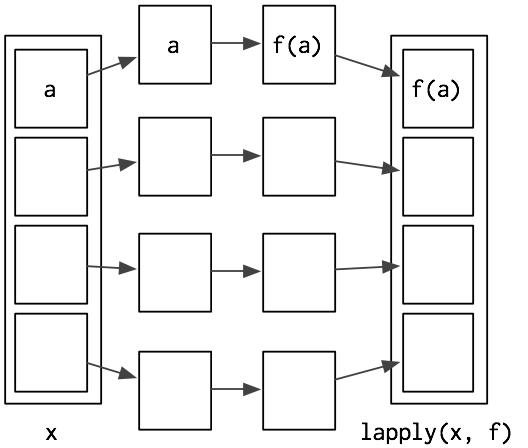
\includegraphics[width=2.4in]{diagrams/lapply.png}

\texttt{lapply()} is written in C for performance, but we can create a
simple R implementation that does the same thing:

\begin{Shaded}
\begin{Highlighting}[]
\NormalTok{lapply2 <-}\StringTok{ }\NormalTok{function(x, f, ...) \{}
  \NormalTok{out <-}\StringTok{ }\KeywordTok{vector}\NormalTok{(}\StringTok{"list"}\NormalTok{, }\KeywordTok{length}\NormalTok{(x))}
  \NormalTok{for (i in }\KeywordTok{seq_along}\NormalTok{(x)) \{}
    \NormalTok{out[[i]] <-}\StringTok{ }\KeywordTok{f}\NormalTok{(x[[i]], ...)}
  \NormalTok{\}}
  \NormalTok{out}
\NormalTok{\}}
\end{Highlighting}
\end{Shaded}

From this code, you can see that \texttt{lapply()} is a wrapper for a
common for loop pattern: create a container for output, apply
\texttt{f()} to each component of a list, and fill the container with
the results. All other for loop functionals are variations on this
theme: they simply use different types of input or output.

\texttt{lapply()} makes it easier to work with lists by eliminating much
of the boilerplate associated with looping. This allows you to focus on
the function that you're applying:

\begin{Shaded}
\begin{Highlighting}[]
\CommentTok{# Create some random data}
\NormalTok{l <-}\StringTok{ }\KeywordTok{replicate}\NormalTok{(}\DecValTok{20}\NormalTok{, }\KeywordTok{runif}\NormalTok{(}\KeywordTok{sample}\NormalTok{(}\DecValTok{1}\NormalTok{:}\DecValTok{10}\NormalTok{, }\DecValTok{1}\NormalTok{)), }\DataTypeTok{simplify =} \OtherTok{FALSE}\NormalTok{)}

\CommentTok{# With a for loop}
\NormalTok{out <-}\StringTok{ }\KeywordTok{vector}\NormalTok{(}\StringTok{"list"}\NormalTok{, }\KeywordTok{length}\NormalTok{(l))}
\NormalTok{for (i in }\KeywordTok{seq_along}\NormalTok{(l)) \{}
  \NormalTok{out[[i]] <-}\StringTok{ }\KeywordTok{length}\NormalTok{(l[[i]])}
\NormalTok{\}}
\KeywordTok{unlist}\NormalTok{(out)}
\CommentTok{#>  [1] 10  2  1  7  1 10 10  5  3  7  5  1  4 10  2  4  6  3  8}
\CommentTok{#> [20]  2}

\CommentTok{# With lapply}
\KeywordTok{unlist}\NormalTok{(}\KeywordTok{lapply}\NormalTok{(l, length))}
\CommentTok{#>  [1] 10  2  1  7  1 10 10  5  3  7  5  1  4 10  2  4  6  3  8}
\CommentTok{#> [20]  2}
\end{Highlighting}
\end{Shaded}

(I'm using \texttt{unlist()} to convert the output from a list to a
vector to make it more compact. We'll see other ways of making the
output a vector shortly.)

Since data frames are also lists, \texttt{lapply()} is also useful when
you want to do something to each column of a data frame:
\index{data frames!modifying each column}

\begin{Shaded}
\begin{Highlighting}[]
\CommentTok{# What class is each column?}
\KeywordTok{unlist}\NormalTok{(}\KeywordTok{lapply}\NormalTok{(mtcars, class))}
\CommentTok{#>       mpg       cyl      disp        hp      drat        wt }
\CommentTok{#> "numeric" "numeric" "numeric" "numeric" "numeric" "numeric" }
\CommentTok{#>      qsec        vs        am      gear      carb }
\CommentTok{#> "numeric" "numeric" "numeric" "numeric" "numeric"}

\CommentTok{# Divide each column by the mean}
\NormalTok{mtcars[] <-}\StringTok{ }\KeywordTok{lapply}\NormalTok{(mtcars, function(x) x /}\StringTok{ }\KeywordTok{mean}\NormalTok{(x))}
\end{Highlighting}
\end{Shaded}

The pieces of \texttt{x} are always supplied as the first argument to
\texttt{f}. If you want to vary a different argument, you can use an
anonymous function. The following example varies the amount of trimming
applied when computing the mean of a fixed \texttt{x}.

\begin{Shaded}
\begin{Highlighting}[]
\NormalTok{trims <-}\StringTok{ }\KeywordTok{c}\NormalTok{(}\DecValTok{0}\NormalTok{, }\FloatTok{0.1}\NormalTok{, }\FloatTok{0.2}\NormalTok{, }\FloatTok{0.5}\NormalTok{)}
\NormalTok{x <-}\StringTok{ }\KeywordTok{rcauchy}\NormalTok{(}\DecValTok{1000}\NormalTok{)}
\KeywordTok{unlist}\NormalTok{(}\KeywordTok{lapply}\NormalTok{(trims, function(trim) }\KeywordTok{mean}\NormalTok{(x, }\DataTypeTok{trim =} \NormalTok{trim)))}
\CommentTok{#> [1] -20.89074  -0.01300   0.02146   0.04547}
\end{Highlighting}
\end{Shaded}

\subsection{Looping patterns}

It's useful to remember that there are three basic ways to loop over a
vector: \index{loops!common patterns}

\begin{enumerate}
\def\labelenumi{\arabic{enumi}.}
\itemsep1pt\parskip0pt\parsep0pt
\item
  loop over the elements: \texttt{for (x in xs)}
\item
  loop over the numeric indices: \texttt{for (i in seq\_along(xs))}
\item
  loop over the names: \texttt{for (nm in names(xs))}
\end{enumerate}

The first form is usually not a good choice for a for loop because it
leads to inefficient ways of saving output. With this form it's very
natural to save the output by extending a datastructure, like in this
example:

\begin{Shaded}
\begin{Highlighting}[]
\NormalTok{xs <-}\StringTok{ }\KeywordTok{runif}\NormalTok{(}\FloatTok{1e3}\NormalTok{)}
\NormalTok{res <-}\StringTok{ }\KeywordTok{c}\NormalTok{()}
\NormalTok{for (x in xs) \{}
  \CommentTok{# This is slow!}
  \NormalTok{res <-}\StringTok{ }\KeywordTok{c}\NormalTok{(res, }\KeywordTok{sqrt}\NormalTok{(x))}
\NormalTok{\}}
\end{Highlighting}
\end{Shaded}

This is slow because each time you extend the vector, R has to copy all
of the existing elements. \hyperref[avoid-copies]{Avoid copies}
discusses this problem in more depth. Instead, it's much better to
create the space you'll need for the output and then fill it in. This is
easiest with the second form: \index{avoiding copies}

\begin{Shaded}
\begin{Highlighting}[]
\NormalTok{res <-}\StringTok{ }\KeywordTok{numeric}\NormalTok{(}\KeywordTok{length}\NormalTok{(xs))}
\NormalTok{for (i in }\KeywordTok{seq_along}\NormalTok{(xs)) \{}
  \NormalTok{res[i] <-}\StringTok{ }\KeywordTok{sqrt}\NormalTok{(xs[i])}
\NormalTok{\}}
\end{Highlighting}
\end{Shaded}

Just as there are three basic ways to use a for loop, there are three
basic ways to use \texttt{lapply()}:

\begin{Shaded}
\begin{Highlighting}[]
\KeywordTok{lapply}\NormalTok{(xs, function(x) \{\})}
\KeywordTok{lapply}\NormalTok{(}\KeywordTok{seq_along}\NormalTok{(xs), function(i) \{\})}
\KeywordTok{lapply}\NormalTok{(}\KeywordTok{names}\NormalTok{(xs), function(nm) \{\})}
\end{Highlighting}
\end{Shaded}

Typically you'd use the first form because \texttt{lapply()} takes care
of saving the output for you. However, if you need to know the position
or name of the element you're working with, you should use the second or
third form. Both give you an element's position (\texttt{i},
\texttt{nm}) and value (\texttt{xs{[}{[}i{]}{]}},
\texttt{xs{[}{[}nm{]}{]}}). If you're struggling to solve a problem
using one form, you might find it easier with another.

\subsection{Exercises}

\begin{enumerate}
\def\labelenumi{\arabic{enumi}.}
\item
  Why are the following two invocations of \texttt{lapply()} equivalent?

\begin{Shaded}
\begin{Highlighting}[]
\NormalTok{trims <-}\StringTok{ }\KeywordTok{c}\NormalTok{(}\DecValTok{0}\NormalTok{, }\FloatTok{0.1}\NormalTok{, }\FloatTok{0.2}\NormalTok{, }\FloatTok{0.5}\NormalTok{)}
\NormalTok{x <-}\StringTok{ }\KeywordTok{rcauchy}\NormalTok{(}\DecValTok{100}\NormalTok{)}

\KeywordTok{lapply}\NormalTok{(trims, function(trim) }\KeywordTok{mean}\NormalTok{(x, }\DataTypeTok{trim =} \NormalTok{trim))}
\KeywordTok{lapply}\NormalTok{(trims, mean, }\DataTypeTok{x =} \NormalTok{x)}
\end{Highlighting}
\end{Shaded}
\item
  The function below scales a vector so it falls in the range {[}0,
  1{]}. How would you apply it to every column of a data frame? How
  would you apply it to every numeric column in a data frame?

\begin{Shaded}
\begin{Highlighting}[]
\NormalTok{scale01 <-}\StringTok{ }\NormalTok{function(x) \{}
  \NormalTok{rng <-}\StringTok{ }\KeywordTok{range}\NormalTok{(x, }\DataTypeTok{na.rm =} \OtherTok{TRUE}\NormalTok{)}
  \NormalTok{(x -}\StringTok{ }\NormalTok{rng[}\DecValTok{1}\NormalTok{]) /}\StringTok{ }\NormalTok{(rng[}\DecValTok{2}\NormalTok{] -}\StringTok{ }\NormalTok{rng[}\DecValTok{1}\NormalTok{])}
\NormalTok{\}}
\end{Highlighting}
\end{Shaded}
\item
  Use both for loops and \texttt{lapply()} to fit linear models to the
  \texttt{mtcars} using the formulas stored in this list:

\begin{Shaded}
\begin{Highlighting}[]
\NormalTok{formulas <-}\StringTok{ }\KeywordTok{list}\NormalTok{(}
  \NormalTok{mpg ~}\StringTok{ }\NormalTok{disp,}
  \NormalTok{mpg ~}\StringTok{ }\KeywordTok{I}\NormalTok{(}\DecValTok{1} \NormalTok{/}\StringTok{ }\NormalTok{disp),}
  \NormalTok{mpg ~}\StringTok{ }\NormalTok{disp +}\StringTok{ }\NormalTok{wt,}
  \NormalTok{mpg ~}\StringTok{ }\KeywordTok{I}\NormalTok{(}\DecValTok{1} \NormalTok{/}\StringTok{ }\NormalTok{disp) +}\StringTok{ }\NormalTok{wt}
\NormalTok{)}
\end{Highlighting}
\end{Shaded}
\item
  Fit the model \texttt{mpg \textasciitilde{} disp} to each of the
  bootstrap replicates of \texttt{mtcars} in the list below by using a
  for loop and \texttt{lapply()}. Can you do it without an anonymous
  function?

\begin{Shaded}
\begin{Highlighting}[]
\NormalTok{bootstraps <-}\StringTok{ }\KeywordTok{lapply}\NormalTok{(}\DecValTok{1}\NormalTok{:}\DecValTok{10}\NormalTok{, function(i) \{}
  \NormalTok{rows <-}\StringTok{ }\KeywordTok{sample}\NormalTok{(}\DecValTok{1}\NormalTok{:}\KeywordTok{nrow}\NormalTok{(mtcars), }\DataTypeTok{rep =} \OtherTok{TRUE}\NormalTok{)}
  \NormalTok{mtcars[rows, ]}
\NormalTok{\})}
\end{Highlighting}
\end{Shaded}
\item
  For each model in the previous two exercises, extract $R^2$ using the
  function below.

\begin{Shaded}
\begin{Highlighting}[]
\NormalTok{rsq <-}\StringTok{ }\NormalTok{function(mod) }\KeywordTok{summary}\NormalTok{(mod)$r.squared}
\end{Highlighting}
\end{Shaded}
\end{enumerate}

\hyperdef{}{functionals-loop}{\section{For loop functionals: friends of
lapply()}\label{functionals-loop}}

The key to using functionals in place of for loops is recognising that
common looping patterns are already implemented in existing base
functionals. Once you've mastered these existing functionals, the next
step is to start writing your own: if you discover you're duplicating
the same looping pattern in many places, you should extract it out into
its own function.

The following sections build on \texttt{lapply()} and discuss:

\begin{itemize}
\item
  \texttt{sapply()} and \texttt{vapply()}, variants of \texttt{lapply()}
  that produce vectors, matrices, and arrays as \textbf{output}, instead
  of lists.
\item
  \texttt{Map()} and \texttt{mapply()} which iterate over multiple
  \textbf{input} data structures in parallel.
\item
  \texttt{mclapply()} and \texttt{mcMap()}, parallel versions of
  \texttt{lapply()} and \texttt{Map()}.
\item
  Writing a new function, \texttt{rollapply()}, to solve a new problem.
\end{itemize}

\subsection{Vector output: \texttt{sapply} and \texttt{vapply}}

\texttt{sapply()} and \texttt{vapply()} are very similar to
\texttt{lapply()} except they simplify their output to produce an atomic
vector. While \texttt{sapply()} guesses, \texttt{vapply()} takes an
additional argument specifying the output type. \texttt{sapply()} is
great for interactive use because it saves typing, but if you use it
inside your functions you'll get weird errors if you supply the wrong
type of input. \texttt{vapply()} is more verbose, but gives more
informative error messages and never fails silently. It is better suited
for use inside other functions. \indexc{sapply()} \indexc{vapply()}

The following example illustrates these differences. When given a data
frame, \texttt{sapply()} and \texttt{vapply()} return the same results.
When given an empty list, \texttt{sapply()} returns another empty list
instead of the more correct zero-length logical vector.

\begin{Shaded}
\begin{Highlighting}[]
\KeywordTok{sapply}\NormalTok{(mtcars, is.numeric)}
\CommentTok{#>  mpg  cyl disp   hp drat   wt qsec   vs   am gear carb }
\CommentTok{#> TRUE TRUE TRUE TRUE TRUE TRUE TRUE TRUE TRUE TRUE TRUE}
\KeywordTok{vapply}\NormalTok{(mtcars, is.numeric, }\KeywordTok{logical}\NormalTok{(}\DecValTok{1}\NormalTok{))}
\CommentTok{#>  mpg  cyl disp   hp drat   wt qsec   vs   am gear carb }
\CommentTok{#> TRUE TRUE TRUE TRUE TRUE TRUE TRUE TRUE TRUE TRUE TRUE}
\KeywordTok{sapply}\NormalTok{(}\KeywordTok{list}\NormalTok{(), is.numeric)}
\CommentTok{#> list()}
\KeywordTok{vapply}\NormalTok{(}\KeywordTok{list}\NormalTok{(), is.numeric, }\KeywordTok{logical}\NormalTok{(}\DecValTok{1}\NormalTok{))}
\CommentTok{#> logical(0)}
\end{Highlighting}
\end{Shaded}

If the function returns results of different types or lengths,
\texttt{sapply()} will silently return a list, while \texttt{vapply()}
will throw an error. \texttt{sapply()} is fine for interactive use
because you'll normally notice if something goes wrong, but it's
dangerous when writing functions.

The following example illustrates a possible problem when extracting the
class of columns in data frame: if you falsely assume that class only
has one value and use \texttt{sapply()}, you won't find out about the
problem until some future function is given a list instead of a
character vector.

\begin{Shaded}
\begin{Highlighting}[]
\NormalTok{df <-}\StringTok{ }\KeywordTok{data.frame}\NormalTok{(}\DataTypeTok{x =} \DecValTok{1}\NormalTok{:}\DecValTok{10}\NormalTok{, }\DataTypeTok{y =} \NormalTok{letters[}\DecValTok{1}\NormalTok{:}\DecValTok{10}\NormalTok{])}
\KeywordTok{sapply}\NormalTok{(df, class)}
\CommentTok{#>         x         y }
\CommentTok{#> "integer"  "factor"}
\KeywordTok{vapply}\NormalTok{(df, class, }\KeywordTok{character}\NormalTok{(}\DecValTok{1}\NormalTok{))}
\CommentTok{#>         x         y }
\CommentTok{#> "integer"  "factor"}

\NormalTok{df2 <-}\StringTok{ }\KeywordTok{data.frame}\NormalTok{(}\DataTypeTok{x =} \DecValTok{1}\NormalTok{:}\DecValTok{10}\NormalTok{, }\DataTypeTok{y =} \KeywordTok{Sys.time}\NormalTok{() +}\StringTok{ }\DecValTok{1}\NormalTok{:}\DecValTok{10}\NormalTok{)}
\KeywordTok{sapply}\NormalTok{(df2, class)}
\CommentTok{#> $x}
\CommentTok{#> [1] "integer"}
\CommentTok{#> }
\CommentTok{#> $y}
\CommentTok{#> [1] "POSIXct" "POSIXt"}
\KeywordTok{vapply}\NormalTok{(df2, class, }\KeywordTok{character}\NormalTok{(}\DecValTok{1}\NormalTok{))}
\CommentTok{#> Error: values must be length 1,}
\CommentTok{#>  but FUN(X[[2]]) result is length 2}
\end{Highlighting}
\end{Shaded}

\texttt{sapply()} is a thin wrapper around \texttt{lapply()} that
transforms a list into a vector in the final step. \texttt{vapply()} is
an implementation of \texttt{lapply()} that assigns results to a vector
(or matrix) of appropriate type instead of as a list. The following code
shows a pure R implementation of the essence of \texttt{sapply()} and
\texttt{vapply()} (the real functions have better error handling and
preserve names, among other things).

\begin{Shaded}
\begin{Highlighting}[]
\NormalTok{sapply2 <-}\StringTok{ }\NormalTok{function(x, f, ...) \{}
  \NormalTok{res <-}\StringTok{ }\KeywordTok{lapply2}\NormalTok{(x, f, ...)}
  \KeywordTok{simplify2array}\NormalTok{(res)}
\NormalTok{\}}

\NormalTok{vapply2 <-}\StringTok{ }\NormalTok{function(x, f, f.value, ...) \{}
  \NormalTok{out <-}\StringTok{ }\KeywordTok{matrix}\NormalTok{(}\KeywordTok{rep}\NormalTok{(f.value, }\KeywordTok{length}\NormalTok{(x)), }\DataTypeTok{nrow =} \KeywordTok{length}\NormalTok{(x))}
  \NormalTok{for (i in }\KeywordTok{seq_along}\NormalTok{(x)) \{}
    \NormalTok{res <-}\StringTok{ }\KeywordTok{f}\NormalTok{(x[i], ...)}
    \KeywordTok{stopifnot}\NormalTok{(}
      \KeywordTok{length}\NormalTok{(res) ==}\StringTok{ }\KeywordTok{length}\NormalTok{(f.value),}
      \KeywordTok{typeof}\NormalTok{(res) ==}\StringTok{ }\KeywordTok{typeof}\NormalTok{(f.value)}
    \NormalTok{)}
    \NormalTok{out[i, ] <-}\StringTok{ }\NormalTok{res}
  \NormalTok{\}}
  \NormalTok{out}
\NormalTok{\}}
\end{Highlighting}
\end{Shaded}

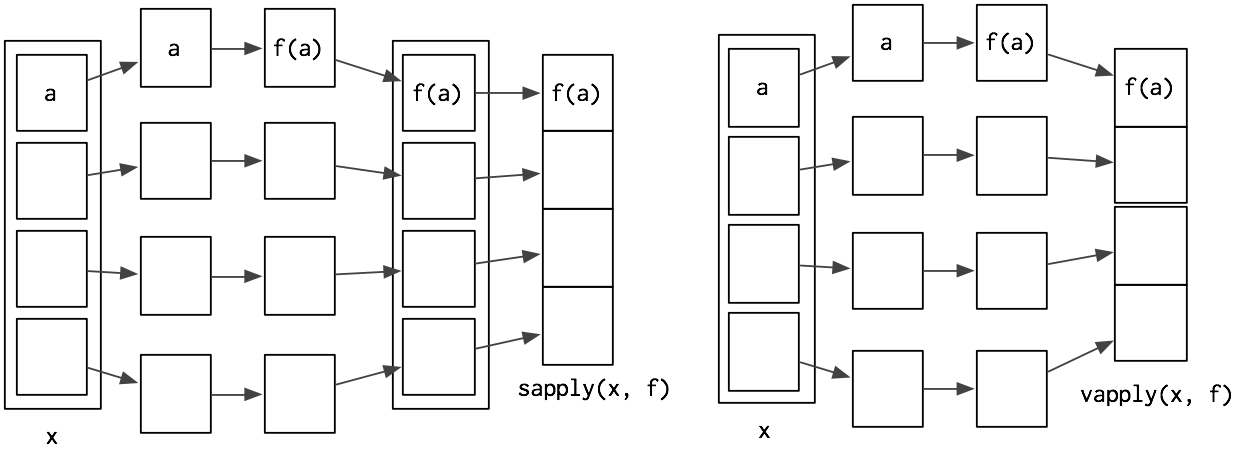
\includegraphics[width=4.35in]{diagrams/sapply-vapply.png}

\texttt{vapply()} and \texttt{sapply()} have different outputs from
\texttt{lapply()}. The following section discusses \texttt{Map()}, which
has different inputs.

\subsection{Multiple inputs: \texttt{Map} (and
\texttt{mapply})}\label{map}

With \texttt{lapply()}, only one argument to the function varies; the
others are fixed. This makes it poorly suited for some problems. For
example, how would you find a weighted mean when you have two lists, one
of observations and the other of weights? \indexc{Map()}

\begin{Shaded}
\begin{Highlighting}[]
\CommentTok{# Generate some sample data}
\NormalTok{xs <-}\StringTok{ }\KeywordTok{replicate}\NormalTok{(}\DecValTok{5}\NormalTok{, }\KeywordTok{runif}\NormalTok{(}\DecValTok{10}\NormalTok{), }\DataTypeTok{simplify =} \OtherTok{FALSE}\NormalTok{)}
\NormalTok{ws <-}\StringTok{ }\KeywordTok{replicate}\NormalTok{(}\DecValTok{5}\NormalTok{, }\KeywordTok{rpois}\NormalTok{(}\DecValTok{10}\NormalTok{, }\DecValTok{5}\NormalTok{) +}\StringTok{ }\DecValTok{1}\NormalTok{, }\DataTypeTok{simplify =} \OtherTok{FALSE}\NormalTok{)}
\end{Highlighting}
\end{Shaded}

It's easy to use \texttt{lapply()} to compute the unweighted means:

\begin{Shaded}
\begin{Highlighting}[]
\KeywordTok{unlist}\NormalTok{(}\KeywordTok{lapply}\NormalTok{(xs, mean))}
\CommentTok{#> [1] 0.6134 0.5228 0.4685 0.5108 0.5004}
\end{Highlighting}
\end{Shaded}

But how could we supply the weights to \texttt{weighted.mean()}?
\texttt{lapply(x, means, w)} won't work because the additional arguments
to \texttt{lapply()} are passed to every call. We could change looping
forms:

\begin{Shaded}
\begin{Highlighting}[]
\KeywordTok{unlist}\NormalTok{(}\KeywordTok{lapply}\NormalTok{(}\KeywordTok{seq_along}\NormalTok{(xs), function(i) \{}
  \KeywordTok{weighted.mean}\NormalTok{(xs[[i]], ws[[i]])}
\NormalTok{\}))}
\CommentTok{#> [1] 0.6659 0.4797 0.4326 0.4845 0.5218}
\end{Highlighting}
\end{Shaded}

This works, but it's a little clumsy. A cleaner alternative is to use
\texttt{Map}, a variant of \texttt{lapply()}, where all arguments can
vary. This lets us write:

\begin{Shaded}
\begin{Highlighting}[]
\KeywordTok{unlist}\NormalTok{(}\KeywordTok{Map}\NormalTok{(weighted.mean, xs, ws))}
\CommentTok{#> [1] 0.6659 0.4797 0.4326 0.4845 0.5218}
\end{Highlighting}
\end{Shaded}

Note that the order of arguments is a little different: function is the
first argument for \texttt{Map()} and the second for \texttt{lapply()}.

This is equivalent to:

\begin{Shaded}
\begin{Highlighting}[]
\KeywordTok{stopifnot}\NormalTok{(}\KeywordTok{length}\NormalTok{(xs) ==}\StringTok{ }\KeywordTok{length}\NormalTok{(ws))}
\NormalTok{out <-}\StringTok{ }\KeywordTok{vector}\NormalTok{(}\StringTok{"list"}\NormalTok{, }\KeywordTok{length}\NormalTok{(xs))}
\NormalTok{for (i in }\KeywordTok{seq_along}\NormalTok{(xs)) \{}
  \NormalTok{out[[i]] <-}\StringTok{ }\KeywordTok{weighted.mean}\NormalTok{(xs[[i]], ws[[i]])}
\NormalTok{\}}
\end{Highlighting}
\end{Shaded}

There's a natural equivalence between \texttt{Map()} and
\texttt{lapply()} because you can always convert a \texttt{Map()} to an
\texttt{lapply()} that iterates over indices. But using \texttt{Map()}
is more concise, and more clearly indicates what you're trying to do.

\texttt{Map} is useful whenever you have two (or more) lists (or data
frames) that you need to process in parallel. For example, another way
of standardising columns is to first compute the means and then divide
by them. We could do this with \texttt{lapply()}, but if we do it in two
steps, we can more easily check the results at each step, which is
particularly important if the first step is more complicated.

\begin{Shaded}
\begin{Highlighting}[]
\NormalTok{mtmeans <-}\StringTok{ }\KeywordTok{lapply}\NormalTok{(mtcars, mean)}
\NormalTok{mtmeans[] <-}\StringTok{ }\KeywordTok{Map}\NormalTok{(}\StringTok{`}\DataTypeTok{/}\StringTok{`}\NormalTok{, mtcars, mtmeans)}

\CommentTok{# In this case, equivalent to}
\NormalTok{mtcars[] <-}\StringTok{ }\KeywordTok{lapply}\NormalTok{(mtcars, function(x) x /}\StringTok{ }\KeywordTok{mean}\NormalTok{(x))}
\end{Highlighting}
\end{Shaded}

If some of the arguments should be fixed and constant, use an anonymous
function:

\begin{Shaded}
\begin{Highlighting}[]
\KeywordTok{Map}\NormalTok{(function(x, w) }\KeywordTok{weighted.mean}\NormalTok{(x, w, }\DataTypeTok{na.rm =} \OtherTok{TRUE}\NormalTok{), xs, ws)}
\end{Highlighting}
\end{Shaded}

We'll see a more compact way to express the same idea in the next
chapter.

\begin{shortbox}\Boxhead{mapply}

You may be more familiar with \texttt{mapply()} than \texttt{Map()}. I
prefer \texttt{Map()} because:

\begin{itemize}
\item
  It's equivalent to \texttt{mapply} with \texttt{simplify = FALSE},
  which is almost always what you want.
\item
  Instead of using an anonymous function to provide constant inputs,
  \texttt{mapply} has the \texttt{MoreArgs} argument that takes a list
  of extra arguments that will be supplied, as is, to each call. This
  breaks R's usual lazy evaluation semantics, and is inconsistent with
  other functions.
\end{itemize}

In brief, \texttt{mapply()} adds more complication for little gain.
\indexc{mapply()}

\end{shortbox}

\subsection{Rolling computations}

What if you need a for loop replacement that doesn't exist in base R?
You can often create your own by recognising common looping structures
and implementing your own wrapper. For example, you might be interested
in smoothing your data using a rolling (or running) mean function:
\index{rolling calculation}

\begin{Shaded}
\begin{Highlighting}[]
\NormalTok{rollmean <-}\StringTok{ }\NormalTok{function(x, n) \{}
  \NormalTok{out <-}\StringTok{ }\KeywordTok{rep}\NormalTok{(}\OtherTok{NA}\NormalTok{, }\KeywordTok{length}\NormalTok{(x))}

  \NormalTok{offset <-}\StringTok{ }\KeywordTok{trunc}\NormalTok{(n /}\StringTok{ }\DecValTok{2}\NormalTok{)}
  \NormalTok{for (i in (offset +}\StringTok{ }\DecValTok{1}\NormalTok{):(}\KeywordTok{length}\NormalTok{(x) -}\StringTok{ }\NormalTok{n +}\StringTok{ }\NormalTok{offset -}\StringTok{ }\DecValTok{1}\NormalTok{)) \{}
    \NormalTok{out[i] <-}\StringTok{ }\KeywordTok{mean}\NormalTok{(x[(i -}\StringTok{ }\NormalTok{offset):(i +}\StringTok{ }\NormalTok{offset -}\StringTok{ }\DecValTok{1}\NormalTok{)])}
  \NormalTok{\}}
  \NormalTok{out}
\NormalTok{\}}
\NormalTok{x <-}\StringTok{ }\KeywordTok{seq}\NormalTok{(}\DecValTok{1}\NormalTok{, }\DecValTok{3}\NormalTok{, }\DataTypeTok{length =} \FloatTok{1e2}\NormalTok{) +}\StringTok{ }\KeywordTok{runif}\NormalTok{(}\FloatTok{1e2}\NormalTok{)}
\KeywordTok{plot}\NormalTok{(x)}
\KeywordTok{lines}\NormalTok{(}\KeywordTok{rollmean}\NormalTok{(x, }\DecValTok{5}\NormalTok{), }\DataTypeTok{col =} \StringTok{"blue"}\NormalTok{, }\DataTypeTok{lwd =} \DecValTok{2}\NormalTok{)}
\KeywordTok{lines}\NormalTok{(}\KeywordTok{rollmean}\NormalTok{(x, }\DecValTok{10}\NormalTok{), }\DataTypeTok{col =} \StringTok{"red"}\NormalTok{, }\DataTypeTok{lwd =} \DecValTok{2}\NormalTok{)}
\end{Highlighting}
\end{Shaded}

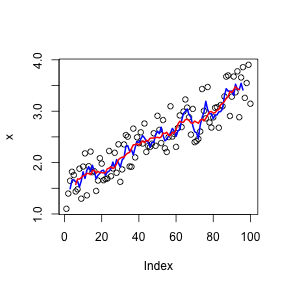
\includegraphics{figures/roll-mean.pdf}

But if the noise was more variable (i.e., it has a longer tail), you
might worry that your rolling mean was too sensitive to outliers.
Instead, you might want to compute a rolling median.

\begin{Shaded}
\begin{Highlighting}[]
\NormalTok{x <-}\StringTok{ }\KeywordTok{seq}\NormalTok{(}\DecValTok{1}\NormalTok{, }\DecValTok{3}\NormalTok{, }\DataTypeTok{length =} \FloatTok{1e2}\NormalTok{) +}\StringTok{ }\KeywordTok{rt}\NormalTok{(}\FloatTok{1e2}\NormalTok{, }\DataTypeTok{df =} \DecValTok{2}\NormalTok{) /}\StringTok{ }\DecValTok{3}
\KeywordTok{plot}\NormalTok{(x)}
\KeywordTok{lines}\NormalTok{(}\KeywordTok{rollmean}\NormalTok{(x, }\DecValTok{5}\NormalTok{), }\DataTypeTok{col =} \StringTok{"red"}\NormalTok{, }\DataTypeTok{lwd =} \DecValTok{2}\NormalTok{)}
\end{Highlighting}
\end{Shaded}

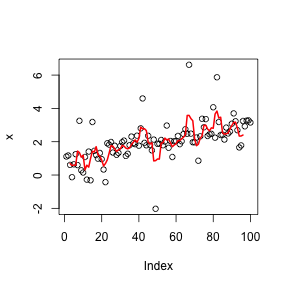
\includegraphics{figures/outliers.pdf}

To change \texttt{rollmean()} to \texttt{rollmedian()}, all you need to
do is replace \texttt{mean} with \texttt{median} inside the loop. But
instead of copying and pasting to create a new function, we could
extract the idea of computing a rolling summary into its own function:
\indexc{rollapply()}

\begin{Shaded}
\begin{Highlighting}[]
\NormalTok{rollapply <-}\StringTok{ }\NormalTok{function(x, n, f, ...) \{}
  \NormalTok{out <-}\StringTok{ }\KeywordTok{rep}\NormalTok{(}\OtherTok{NA}\NormalTok{, }\KeywordTok{length}\NormalTok{(x))}

  \NormalTok{offset <-}\StringTok{ }\KeywordTok{trunc}\NormalTok{(n /}\StringTok{ }\DecValTok{2}\NormalTok{)}
  \NormalTok{for (i in (offset +}\StringTok{ }\DecValTok{1}\NormalTok{):(}\KeywordTok{length}\NormalTok{(x) -}\StringTok{ }\NormalTok{n +}\StringTok{ }\NormalTok{offset +}\StringTok{ }\DecValTok{1}\NormalTok{)) \{}
    \NormalTok{out[i] <-}\StringTok{ }\KeywordTok{f}\NormalTok{(x[(i -}\StringTok{ }\NormalTok{offset):(i +}\StringTok{ }\NormalTok{offset)], ...)}
  \NormalTok{\}}
  \NormalTok{out}
\NormalTok{\}}
\KeywordTok{plot}\NormalTok{(x)}
\KeywordTok{lines}\NormalTok{(}\KeywordTok{rollapply}\NormalTok{(x, }\DecValTok{5}\NormalTok{, median), }\DataTypeTok{col =} \StringTok{"red"}\NormalTok{, }\DataTypeTok{lwd =} \DecValTok{2}\NormalTok{)}
\end{Highlighting}
\end{Shaded}

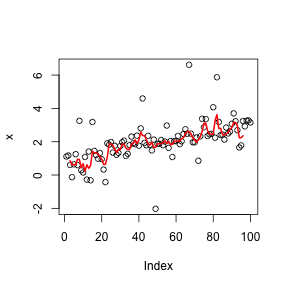
\includegraphics{figures/roll-apply.pdf}

You might notice that the internal loop looks pretty similar to a
\texttt{vapply()} loop, so we could rewrite the function as:

\begin{Shaded}
\begin{Highlighting}[]
\NormalTok{rollapply <-}\StringTok{ }\NormalTok{function(x, n, f, ...) \{}
  \NormalTok{offset <-}\StringTok{ }\KeywordTok{trunc}\NormalTok{(n /}\StringTok{ }\DecValTok{2}\NormalTok{)}
  \NormalTok{locs <-}\StringTok{ }\NormalTok{(offset +}\StringTok{ }\DecValTok{1}\NormalTok{):(}\KeywordTok{length}\NormalTok{(x) -}\StringTok{ }\NormalTok{n +}\StringTok{ }\NormalTok{offset +}\StringTok{ }\DecValTok{1}\NormalTok{)}
  \NormalTok{num <-}\StringTok{ }\KeywordTok{vapply}\NormalTok{(}
    \NormalTok{locs, }
    \NormalTok{function(i) }\KeywordTok{f}\NormalTok{(x[(i -}\StringTok{ }\NormalTok{offset):(i +}\StringTok{ }\NormalTok{offset)], ...),}
    \KeywordTok{numeric}\NormalTok{(}\DecValTok{1}\NormalTok{)}
  \NormalTok{)}

  \KeywordTok{c}\NormalTok{(}\KeywordTok{rep}\NormalTok{(}\OtherTok{NA}\NormalTok{, offset), num)}
\NormalTok{\}}
\end{Highlighting}
\end{Shaded}

This is effectively the same as the implementation in
\texttt{zoo::rollapply()}, which provides many more features and much
more error checking.

\subsection{Parallelisation}

One interesting thing about the implementation of \texttt{lapply()} is
that because each iteration is isolated from all others, the order in
which they are computed doesn't matter. For example, \texttt{lapply3()}
scrambles the order of computation, but the results are always the same:
\index{parallel computing} \index{multicore}

\begin{Shaded}
\begin{Highlighting}[]
\NormalTok{lapply3 <-}\StringTok{ }\NormalTok{function(x, f, ...) \{}
  \NormalTok{out <-}\StringTok{ }\KeywordTok{vector}\NormalTok{(}\StringTok{"list"}\NormalTok{, }\KeywordTok{length}\NormalTok{(x))}
  \NormalTok{for (i in }\KeywordTok{sample}\NormalTok{(}\KeywordTok{seq_along}\NormalTok{(x))) \{}
    \NormalTok{out[[i]] <-}\StringTok{ }\KeywordTok{f}\NormalTok{(x[[i]], ...)}
  \NormalTok{\}}
  \NormalTok{out}
\NormalTok{\}}
\KeywordTok{unlist}\NormalTok{(}\KeywordTok{lapply}\NormalTok{(}\DecValTok{1}\NormalTok{:}\DecValTok{10}\NormalTok{, sqrt))}
\CommentTok{#>  [1] 1.000 1.414 1.732 2.000 2.236 2.449 2.646 2.828 3.000}
\CommentTok{#> [10] 3.162}
\KeywordTok{unlist}\NormalTok{(}\KeywordTok{lapply3}\NormalTok{(}\DecValTok{1}\NormalTok{:}\DecValTok{10}\NormalTok{, sqrt))}
\CommentTok{#>  [1] 1.000 1.414 1.732 2.000 2.236 2.449 2.646 2.828 3.000}
\CommentTok{#> [10] 3.162}
\end{Highlighting}
\end{Shaded}

This has a very important consequence: since we can compute each element
in any order, it's easy to dispatch the tasks to different cores, and
compute them in parallel. This is what \texttt{parallel::mclapply()}
(and \texttt{parallel::mcMap()}) does. (These functions are not
available in Windows, but you can use the similar \texttt{parLapply()}
with a bit more work. See \hyperref[parallelise]{parallelise} for more
details.) \indexc{mclapply()}

\begin{Shaded}
\begin{Highlighting}[]
\KeywordTok{library}\NormalTok{(parallel)}
\KeywordTok{unlist}\NormalTok{(}\KeywordTok{mclapply}\NormalTok{(}\DecValTok{1}\NormalTok{:}\DecValTok{10}\NormalTok{, sqrt, }\DataTypeTok{mc.cores =} \DecValTok{4}\NormalTok{))}
\CommentTok{#>  [1] 1.000 1.414 1.732 2.000 2.236 2.449 2.646 2.828 3.000}
\CommentTok{#> [10] 3.162}
\end{Highlighting}
\end{Shaded}

In this case, \texttt{mclapply()} is actually slower than
\texttt{lapply()}. This is because the cost of the individual
computations is low, and additional work is needed to send the
computation to the different cores and to collect the results.

If we take a more realistic example, generating bootstrap replicates of
a linear model for example, the advantages are clearer:
\index{bootstrapping}

\begin{Shaded}
\begin{Highlighting}[]
\NormalTok{boot_df <-}\StringTok{ }\NormalTok{function(x) x[}\KeywordTok{sample}\NormalTok{(}\KeywordTok{nrow}\NormalTok{(x), }\DataTypeTok{rep =} \NormalTok{T), ]}
\NormalTok{rsquared <-}\StringTok{ }\NormalTok{function(mod) }\KeywordTok{summary}\NormalTok{(mod)$r.square}
\NormalTok{boot_lm <-}\StringTok{ }\NormalTok{function(i) \{}
  \KeywordTok{rsquared}\NormalTok{(}\KeywordTok{lm}\NormalTok{(mpg ~}\StringTok{ }\NormalTok{wt +}\StringTok{ }\NormalTok{disp, }\DataTypeTok{data =} \KeywordTok{boot_df}\NormalTok{(mtcars)))}
\NormalTok{\}}

\KeywordTok{system.time}\NormalTok{(}\KeywordTok{lapply}\NormalTok{(}\DecValTok{1}\NormalTok{:}\DecValTok{500}\NormalTok{, boot_lm))}
\CommentTok{#>    user  system elapsed }
\CommentTok{#>   0.801   0.005   0.807}
\KeywordTok{system.time}\NormalTok{(}\KeywordTok{mclapply}\NormalTok{(}\DecValTok{1}\NormalTok{:}\DecValTok{500}\NormalTok{, boot_lm, }\DataTypeTok{mc.cores =} \DecValTok{2}\NormalTok{))}
\CommentTok{#>    user  system elapsed }
\CommentTok{#>   0.401   0.031   0.438}
\end{Highlighting}
\end{Shaded}

While increasing the number of cores will not always lead to linear
improvement, switching from \texttt{lapply()} or \texttt{Map()} to its
parallelised forms can dramatically improve computational performance.

\subsection{Exercises}

\begin{enumerate}
\def\labelenumi{\arabic{enumi}.}
\item
  Use \texttt{vapply()} to:

  \begin{enumerate}
  \def\labelenumii{\alph{enumii})}
  \item
    Compute the standard deviation of every column in a numeric data
    frame.
  \item
    Compute the standard deviation of every numeric column in a mixed
    data frame. (Hint: you'll need to use \texttt{vapply()} twice.)
  \end{enumerate}
\item
  Why is using \texttt{sapply()} to get the \texttt{class()} of each
  element in a data frame dangerous?
\item
  The following code simulates the performance of a t-test for
  non-normal data. Use \texttt{sapply()} and an anonymous function to
  extract the p-value from every trial.

\begin{Shaded}
\begin{Highlighting}[]
\NormalTok{trials <-}\StringTok{ }\KeywordTok{replicate}\NormalTok{(}
  \DecValTok{100}\NormalTok{, }
  \KeywordTok{t.test}\NormalTok{(}\KeywordTok{rpois}\NormalTok{(}\DecValTok{10}\NormalTok{, }\DecValTok{10}\NormalTok{), }\KeywordTok{rpois}\NormalTok{(}\DecValTok{7}\NormalTok{, }\DecValTok{10}\NormalTok{)),}
  \DataTypeTok{simplify =} \OtherTok{FALSE}
\NormalTok{)}
\end{Highlighting}
\end{Shaded}

  Extra challenge: get rid of the anonymous function by using
  \texttt{{[}{[}} directly.
\item
  What does \texttt{replicate()} do? What sort of for loop does it
  eliminate? Why do its arguments differ from \texttt{lapply()} and
  friends?
\item
  Implement a version of \texttt{lapply()} that supplies \texttt{FUN}
  with both the name and the value of each component.
\item
  Implement a combination of \texttt{Map()} and \texttt{vapply()} to
  create an \texttt{lapply()} variant that iterates in parallel over all
  of its inputs and stores its outputs in a vector (or a matrix). What
  arguments should the function take?
\item
  Implement \texttt{mcsapply()}, a multicore version of
  \texttt{sapply()}. Can you implement \texttt{mcvapply()}, a parallel
  version of \texttt{vapply()}? Why or why not?
\end{enumerate}

\hyperdef{}{functionals-ds}{\section{Manipulating matrices and data
frames}\label{functionals-ds}}

Functionals can also be used to eliminate loops in common data
manipulation tasks. In this section, we'll give a brief overview of the
available options, hint at how they can help you, and point you in the
right direction to learn more. We'll cover three categories of data
structure functionals:

\begin{itemize}
\item
  \texttt{apply()}, \texttt{sweep()}, and \texttt{outer()} with work
  with matrices.
\item
  \texttt{tapply()} summarises a vector by groups defined by another
  vector.
\item
  the \texttt{plyr} package, which generalises \texttt{tapply()} to make
  it easy to work with data frames, lists, or arrays as inputs, and data
  frames, lists, or arrays as outputs.
\end{itemize}

\subsection{Matrix and array operations}

So far, all the functionals we've seen work with 1d input structures.
The three functionals in this section provide useful tools for working
with higher-dimensional data structures. \texttt{apply()} is a variant
of \texttt{sapply()} that works with matrices and arrays. You can think
of it as an operation that summarises a matrix or array by collapsing
each row or column to a single number. It has four arguments:
\indexc{apply()}

\begin{itemize}
\itemsep1pt\parskip0pt\parsep0pt
\item
  \texttt{X}, the matrix or array to summarise
\item
  \texttt{MARGIN}, an integer vector giving the dimensions to summarise
  over, 1 = rows, 2 = columns, etc.
\item
  \texttt{FUN}, a summary function
\item
  \texttt{...} other arguments passed on to \texttt{FUN}
\end{itemize}

A typical example of \texttt{apply()} looks like this

\begin{Shaded}
\begin{Highlighting}[]
\NormalTok{a <-}\StringTok{ }\KeywordTok{matrix}\NormalTok{(}\DecValTok{1}\NormalTok{:}\DecValTok{20}\NormalTok{, }\DataTypeTok{nrow =} \DecValTok{5}\NormalTok{)}
\KeywordTok{apply}\NormalTok{(a, }\DecValTok{1}\NormalTok{, mean)}
\CommentTok{#> [1]  8.5  9.5 10.5 11.5 12.5}
\KeywordTok{apply}\NormalTok{(a, }\DecValTok{2}\NormalTok{, mean)}
\CommentTok{#> [1]  3  8 13 18}
\end{Highlighting}
\end{Shaded}

There are a few caveats to using \texttt{apply()}. It doesn't have a
simplify argument, so you can never be completely sure what type of
output you'll get. This means that \texttt{apply()} is not safe to use
inside a function unless you carefully check the inputs.
\texttt{apply()} is also not idempotent in the sense that if the summary
function is the identity operator, the output is not always the same as
the input:

\begin{Shaded}
\begin{Highlighting}[]
\NormalTok{a1 <-}\StringTok{ }\KeywordTok{apply}\NormalTok{(a, }\DecValTok{1}\NormalTok{, identity)}
\KeywordTok{identical}\NormalTok{(a, a1)}
\CommentTok{#> [1] FALSE}
\KeywordTok{identical}\NormalTok{(a, }\KeywordTok{t}\NormalTok{(a1))}
\CommentTok{#> [1] TRUE}
\NormalTok{a2 <-}\StringTok{ }\KeywordTok{apply}\NormalTok{(a, }\DecValTok{2}\NormalTok{, identity)}
\KeywordTok{identical}\NormalTok{(a, a2)}
\CommentTok{#> [1] TRUE}
\end{Highlighting}
\end{Shaded}

(You can put high-dimensional arrays back in the right order using
\texttt{aperm()}, or use \texttt{plyr::aaply()}, which is idempotent.)

\texttt{sweep()} allows you to ``sweep'' out the values of a summary
statistic. It is often used with \texttt{apply()} to standardise arrays.
The following example scales the rows of a matrix so that all values lie
between 0 and 1. \indexc{sweep()}

\begin{Shaded}
\begin{Highlighting}[]
\NormalTok{x <-}\StringTok{ }\KeywordTok{matrix}\NormalTok{(}\KeywordTok{rnorm}\NormalTok{(}\DecValTok{20}\NormalTok{, }\DecValTok{0}\NormalTok{, }\DecValTok{10}\NormalTok{), }\DataTypeTok{nrow =} \DecValTok{4}\NormalTok{)}
\NormalTok{x1 <-}\StringTok{ }\KeywordTok{sweep}\NormalTok{(x, }\DecValTok{1}\NormalTok{, }\KeywordTok{apply}\NormalTok{(x, }\DecValTok{1}\NormalTok{, min), }\StringTok{`}\DataTypeTok{-}\StringTok{`}\NormalTok{)}
\NormalTok{x2 <-}\StringTok{ }\KeywordTok{sweep}\NormalTok{(x1, }\DecValTok{1}\NormalTok{, }\KeywordTok{apply}\NormalTok{(x1, }\DecValTok{1}\NormalTok{, max), }\StringTok{`}\DataTypeTok{/}\StringTok{`}\NormalTok{)}
\end{Highlighting}
\end{Shaded}

The final matrix functional is \texttt{outer()}. It's a little different
in that it takes multiple vector inputs and creates a matrix or array
output where the input function is run over every combination of the
inputs: \indexc{outer()}

\begin{Shaded}
\begin{Highlighting}[]
\CommentTok{# Create a times table}
\KeywordTok{outer}\NormalTok{(}\DecValTok{1}\NormalTok{:}\DecValTok{3}\NormalTok{, }\DecValTok{1}\NormalTok{:}\DecValTok{10}\NormalTok{, }\StringTok{"*"}\NormalTok{)}
\CommentTok{#>      [,1] [,2] [,3] [,4] [,5] [,6] [,7] [,8] [,9] [,10]}
\CommentTok{#> [1,]    1    2    3    4    5    6    7    8    9    10}
\CommentTok{#> [2,]    2    4    6    8   10   12   14   16   18    20}
\CommentTok{#> [3,]    3    6    9   12   15   18   21   24   27    30}
\end{Highlighting}
\end{Shaded}

Good places to learn more about \texttt{apply()} and friends are:

\begin{itemize}
\item
  \href{http://petewerner.blogspot.com/2012/12/using-apply-sapply-lapply-in-r.html}{``Using
  apply, sapply, lapply in R''} by Peter Werner.
\item
  \href{http://rforpublichealth.blogspot.no/2012/09/the-infamous-apply-function.html}{``The
  infamous apply function''} by Slawa Rokicki.
\item
  \href{http://forgetfulfunctor.blogspot.com/2011/07/r-apply-function-tutorial-with-examples.html}{``The
  R apply function - a tutorial with examples''} by axiomOfChoice.
\item
  The stackoverflow question
  \href{http://stackoverflow.com/questions/3505701}{``R Grouping
  functions: \texttt{sapply} vs. \texttt{lapply} vs. \texttt{apply} vs.
  \texttt{tapply} vs. \texttt{by} vs. \texttt{aggregate}''}.
\end{itemize}

\subsection{Group apply}

You can think about \texttt{tapply()} as a generalisation to
\texttt{apply()} that allows for ``ragged'' arrays, arrays where each
row can have a different number of columns. This is often needed when
you're trying to summarise a data set. For example, imagine you've
collected pulse rate data from a medical trial, and you want to compare
the two groups: \indexc{tapply()}

\begin{Shaded}
\begin{Highlighting}[]
\NormalTok{pulse <-}\StringTok{ }\KeywordTok{round}\NormalTok{(}\KeywordTok{rnorm}\NormalTok{(}\DecValTok{22}\NormalTok{, }\DecValTok{70}\NormalTok{, }\DecValTok{10} \NormalTok{/}\StringTok{ }\DecValTok{3}\NormalTok{)) +}\StringTok{ }\KeywordTok{rep}\NormalTok{(}\KeywordTok{c}\NormalTok{(}\DecValTok{0}\NormalTok{, }\DecValTok{5}\NormalTok{), }\KeywordTok{c}\NormalTok{(}\DecValTok{10}\NormalTok{, }\DecValTok{12}\NormalTok{))}
\NormalTok{group <-}\StringTok{ }\KeywordTok{rep}\NormalTok{(}\KeywordTok{c}\NormalTok{(}\StringTok{"A"}\NormalTok{, }\StringTok{"B"}\NormalTok{), }\KeywordTok{c}\NormalTok{(}\DecValTok{10}\NormalTok{, }\DecValTok{12}\NormalTok{))}

\KeywordTok{tapply}\NormalTok{(pulse, group, length)}
\CommentTok{#>  A  B }
\CommentTok{#> 10 12}
\KeywordTok{tapply}\NormalTok{(pulse, group, mean)}
\CommentTok{#>     A     B }
\CommentTok{#> 70.20 75.25}
\end{Highlighting}
\end{Shaded}

\texttt{tapply()} works by creating a ``ragged'' data structure from a
set of inputs, and then applying a function to the individual elements
of that structure. The first task is actually what the \texttt{split()}
function does. It takes two inputs and returns a list which groups
elements together from the first vector according to elements, or
categories, from the second vector:

\begin{Shaded}
\begin{Highlighting}[]
\KeywordTok{split}\NormalTok{(pulse, group)}
\CommentTok{#> $A}
\CommentTok{#>  [1] 78 70 66 71 66 74 70 70 68 69}
\CommentTok{#> }
\CommentTok{#> $B}
\CommentTok{#>  [1] 73 72 68 77 76 73 74 76 82 82 77 73}
\end{Highlighting}
\end{Shaded}

Then \texttt{tapply()} is just the combination of \texttt{split()} and
\texttt{sapply()}:

\begin{Shaded}
\begin{Highlighting}[]
\NormalTok{tapply2 <-}\StringTok{ }\NormalTok{function(x, group, f, ..., }\DataTypeTok{simplify =} \OtherTok{TRUE}\NormalTok{) \{}
  \NormalTok{pieces <-}\StringTok{ }\KeywordTok{split}\NormalTok{(x, group)}
  \KeywordTok{sapply}\NormalTok{(pieces, f, }\DataTypeTok{simplify =} \NormalTok{simplify)}
\NormalTok{\}}
\KeywordTok{tapply2}\NormalTok{(pulse, group, length)}
\CommentTok{#>  A  B }
\CommentTok{#> 10 12}
\KeywordTok{tapply2}\NormalTok{(pulse, group, mean)}
\CommentTok{#>     A     B }
\CommentTok{#> 70.20 75.25}
\end{Highlighting}
\end{Shaded}

Being able to rewrite \texttt{tapply()} as a combination of
\texttt{split()} and \texttt{sapply()} is a good indication that we've
identified some useful building blocks. \indexc{split()}

\subsection{The plyr package}

One challenge with using the base functionals is that they have grown
organically over time, and have been written by multiple authors. This
means that they are not very consistent: \index{plyr}

\begin{itemize}
\item
  With \texttt{tapply()} and \texttt{sapply()}, the simplify argument is
  called \texttt{simplify}. With \texttt{mapply()}, it's called
  \texttt{SIMPLIFY}. With \texttt{apply()}, the argument is absent.
\item
  \texttt{vapply()} is a variant of \texttt{sapply()} that allows you to
  describe what the output should be, but there are no corresponding
  variants for \texttt{tapply()}, \texttt{apply()}, or \texttt{Map()}.
\item
  The first argument of most base functionals is a vector, but the first
  argument in \texttt{Map()} is a function.
\end{itemize}

This makes learning these operators challenging, as you have to memorise
all of the variations. Additionally, if you think about the possible
combinations of input and output types, base R only covers a partial set
of cases:

\begin{longtable}[c]{@{}llll@{}}
\toprule\addlinespace
& list & data frame & array
\\\addlinespace
\midrule\endhead
list & \texttt{lapply()} & & \texttt{sapply()}
\\\addlinespace
data frame & \texttt{by()} & &
\\\addlinespace
array & & & \texttt{apply()}
\\\addlinespace
\bottomrule
\end{longtable}

This was one of the driving motivations behind the creation of the plyr
package. It provides consistently named functions with consistently
named arguments and covers all combinations of input and output data
structures:

\begin{longtable}[c]{@{}llll@{}}
\toprule\addlinespace
& list & data frame & array
\\\addlinespace
\midrule\endhead
list & \texttt{llply()} & \texttt{ldply()} & \texttt{laply()}
\\\addlinespace
data frame & \texttt{dlply()} & \texttt{ddply()} & \texttt{daply()}
\\\addlinespace
array & \texttt{alply()} & \texttt{adply()} & \texttt{aaply()}
\\\addlinespace
\bottomrule
\end{longtable}

Each of these functions splits up the input, applies a function to each
piece, and then combines the results. Overall, this process is called
``split-apply-combine''. You can read more about it and plyr in
\href{http://www.jstatsoft.org/v40/i01/}{``The Split-Apply-Combine
Strategy for Data Analysis''}, an open-access article published in the
\emph{Journal of Statistical Software}.
\index{split-apply-combine strategy}

\subsection{Exercises}

\begin{enumerate}
\def\labelenumi{\arabic{enumi}.}
\item
  How does \texttt{apply()} arrange the output? Read the documentation
  and perform some experiments.
\item
  There's no equivalent to \texttt{split()} + \texttt{vapply()}. Should
  there be? When would it be useful? Implement one yourself.
\item
  Implement a pure R version of \texttt{split()}. (Hint: use
  \texttt{unique()} and subsetting.) Can you do it without a for loop?
\item
  What other types of input and output are missing? Brainstorm before
  you look up some answers in the
  \href{http://www.jstatsoft.org/v40/i01/}{plyr paper}.
\end{enumerate}

\hyperdef{}{functionals-fp}{\section{Manipulating
lists}\label{functionals-fp}}

Another way of thinking about functionals is as a set of general tools
for altering, subsetting, and collapsing lists. Every functional
programming language has three tools for this: \texttt{Map()},
\texttt{Reduce()}, and \texttt{Filter()}. We've seen \texttt{Map()}
already, and the following sections describe \texttt{Reduce()}, a
powerful tool for extending two-argument functions, and
\texttt{Filter()}, a member of an important class of functionals that
work with predicates, functions that return a single \texttt{TRUE} or
\texttt{FALSE}.

\subsection{\texttt{Reduce()}}

\texttt{Reduce()} reduces a vector, \texttt{x}, to a single value by
recursively calling a function, \texttt{f}, two arguments at a time. It
combines the first two elements with \texttt{f}, then combines the
result of that call with the third element, and so on. Calling
\texttt{Reduce(f, 1:3)} is equivalent to \texttt{f(f(1, 2), 3)}. Reduce
is also known as fold, because it folds together adjacent elements in
the list. \indexc{Reduce()} \index{fold}

The following two examples show what \texttt{Reduce} does with an infix
and prefix function:

\begin{Shaded}
\begin{Highlighting}[]
\KeywordTok{Reduce}\NormalTok{(}\StringTok{`}\DataTypeTok{+}\StringTok{`}\NormalTok{, }\DecValTok{1}\NormalTok{:}\DecValTok{3}\NormalTok{) }\CommentTok{# -> ((1 + 2) + 3)}
\KeywordTok{Reduce}\NormalTok{(sum, }\DecValTok{1}\NormalTok{:}\DecValTok{3}\NormalTok{) }\CommentTok{# -> sum(sum(1, 2), 3)}
\end{Highlighting}
\end{Shaded}

The essence of \texttt{Reduce()} can be described by a simple for loop:

\begin{Shaded}
\begin{Highlighting}[]
\NormalTok{Reduce2 <-}\StringTok{ }\NormalTok{function(f, x) \{}
  \NormalTok{out <-}\StringTok{ }\NormalTok{x[[}\DecValTok{1}\NormalTok{]]}
  \NormalTok{for(i in }\KeywordTok{seq}\NormalTok{(}\DecValTok{2}\NormalTok{, }\KeywordTok{length}\NormalTok{(x))) \{}
    \NormalTok{out <-}\StringTok{ }\KeywordTok{f}\NormalTok{(out, x[[i]])}
  \NormalTok{\}}
  \NormalTok{out}
\NormalTok{\}}
\end{Highlighting}
\end{Shaded}

The real \texttt{Reduce()} is more complicated because it includes
arguments to control whether the values are reduced from the left or
from the right (\texttt{right}), an optional initial value
(\texttt{init}), and an option to output intermediate results
(\texttt{accumulate}).

\texttt{Reduce()} is an elegant way of extending a function that works
with two inputs into a function that can deal with any number of inputs.
It's useful for implementing many types of recursive operations, like
merges and intersections. (We'll see another use in the final case
study.) Imagine you have a list of numeric vectors, and you want to find
the values that occur in every element:

\begin{Shaded}
\begin{Highlighting}[]
\NormalTok{l <-}\StringTok{ }\KeywordTok{replicate}\NormalTok{(}\DecValTok{5}\NormalTok{, }\KeywordTok{sample}\NormalTok{(}\DecValTok{1}\NormalTok{:}\DecValTok{10}\NormalTok{, }\DecValTok{15}\NormalTok{, }\DataTypeTok{replace =} \NormalTok{T), }\DataTypeTok{simplify =} \OtherTok{FALSE}\NormalTok{)}
\KeywordTok{str}\NormalTok{(l)}
\CommentTok{#> List of 5}
\CommentTok{#>  $ : int [1:15] 4 8 3 7 5 5 3 4 8 9 ...}
\CommentTok{#>  $ : int [1:15] 10 4 8 6 10 9 3 7 4 6 ...}
\CommentTok{#>  $ : int [1:15] 1 8 3 8 8 4 10 8 3 5 ...}
\CommentTok{#>  $ : int [1:15] 6 10 5 5 2 10 10 4 2 8 ...}
\CommentTok{#>  $ : int [1:15] 6 7 8 10 3 6 9 1 5 1 ...}
\end{Highlighting}
\end{Shaded}

You could do that by intersecting each element in turn:

\begin{Shaded}
\begin{Highlighting}[]
\KeywordTok{intersect}\NormalTok{(}\KeywordTok{intersect}\NormalTok{(}\KeywordTok{intersect}\NormalTok{(}\KeywordTok{intersect}\NormalTok{(l[[}\DecValTok{1}\NormalTok{]], l[[}\DecValTok{2}\NormalTok{]]),}
  \NormalTok{l[[}\DecValTok{3}\NormalTok{]]), l[[}\DecValTok{4}\NormalTok{]]), l[[}\DecValTok{5}\NormalTok{]])}
\CommentTok{#> [1] 4 8 7 6}
\end{Highlighting}
\end{Shaded}

That's hard to read. With \texttt{Reduce()}, the equivalent is:

\begin{Shaded}
\begin{Highlighting}[]
\KeywordTok{Reduce}\NormalTok{(intersect, l)}
\CommentTok{#> [1] 4 8 7 6}
\end{Highlighting}
\end{Shaded}

\subsection{Predicate functionals}

A \textbf{predicate} is a function that returns a single \texttt{TRUE}
or \texttt{FALSE}, like \texttt{is.character}, \texttt{all}, or
\texttt{is.NULL}. A predicate functional applies a predicate to each
element of a list or data frame. There are three useful predicate
functionals in base R: \texttt{Filter()}, \texttt{Find()}, and
\texttt{Position()}. \index{predicates}
\index{functions!predict|see{predicates}}

\begin{itemize}
\item
  \texttt{Filter()} selects only those elements which match the
  predicate. \indexc{Filter()}
\item
  \texttt{Find()} returns the first element which matches the predicate
  (or the last element if \texttt{right = TRUE}). \indexc{Find()}
\item
  \texttt{Position()} returns the position of the first element that
  matches the predicate (or the last element if \texttt{right = TRUE}).
  \indexc{Position()}
\end{itemize}

Another useful predicate functional is \texttt{where()}, a custom
functional generates a logical vector from a list (or a data frame) and
a predicate: \indexc{where()}

\begin{Shaded}
\begin{Highlighting}[]
\NormalTok{where <-}\StringTok{ }\NormalTok{function(f, x) \{}
  \KeywordTok{vapply}\NormalTok{(x, f, }\KeywordTok{logical}\NormalTok{(}\DecValTok{1}\NormalTok{))}
\NormalTok{\}}
\end{Highlighting}
\end{Shaded}

The following example shows how you might use these functionals with a
data frame:

\begin{Shaded}
\begin{Highlighting}[]
\NormalTok{df <-}\StringTok{ }\KeywordTok{data.frame}\NormalTok{(}\DataTypeTok{x =} \DecValTok{1}\NormalTok{:}\DecValTok{3}\NormalTok{, }\DataTypeTok{y =} \KeywordTok{c}\NormalTok{(}\StringTok{"a"}\NormalTok{, }\StringTok{"b"}\NormalTok{, }\StringTok{"c"}\NormalTok{))}
\KeywordTok{where}\NormalTok{(is.factor, df)}
\CommentTok{#>     x     y }
\CommentTok{#> FALSE  TRUE}
\KeywordTok{str}\NormalTok{(}\KeywordTok{Filter}\NormalTok{(is.factor, df))}
\CommentTok{#> 'data.frame':    3 obs. of  1 variable:}
\CommentTok{#>  $ y: Factor w/ 3 levels "a","b","c": 1 2 3}
\KeywordTok{str}\NormalTok{(}\KeywordTok{Find}\NormalTok{(is.factor, df))}
\CommentTok{#>  Factor w/ 3 levels "a","b","c": 1 2 3}
\KeywordTok{Position}\NormalTok{(is.factor, df)}
\CommentTok{#> [1] 2}
\end{Highlighting}
\end{Shaded}

\subsection{Exercises}

\begin{enumerate}
\def\labelenumi{\arabic{enumi}.}
\item
  Why isn't \texttt{is.na()} a predicate function? What base R function
  is closest to being a predicate version of \texttt{is.na()}?
\item
  Use \texttt{Filter()} and \texttt{vapply()} to create a function that
  applies a summary statistic to every numeric column in a data frame.
\item
  What's the relationship between \texttt{which()} and
  \texttt{Position()}? What's the relationship between \texttt{where()}
  and \texttt{Filter()}?
\item
  Implement \texttt{Any()}, a function that takes a list and a predicate
  function, and returns \texttt{TRUE} if the predicate function returns
  \texttt{TRUE} for any of the inputs. Implement \texttt{All()}
  similarly.
\item
  Implement the \texttt{span()} function from Haskell: given a list
  \texttt{x} and a predicate function \texttt{f}, \texttt{span} returns
  the location of the longest sequential run of elements where the
  predicate is true. (Hint: you might find \texttt{rle()} helpful.)
\end{enumerate}

\hyperdef{}{functionals-math}{\section{Mathematical
functionals}\label{functionals-math}}

Functionals are very common in mathematics. The limit, the maximum, the
roots (the set of points where \texttt{f(x) = 0}), and the definite
integral are all functionals: given a function, they return a single
number (or vector of numbers). At first glance, these functions don't
seem to fit in with the theme of eliminating loops, but if you dig
deeper you'll find out that they are all implemented using an algorithm
that involves iteration.

In this section we'll use some of R's built-in mathematical functionals.
There are three functionals that work with functions to return single
numeric values: \indexc{integrate()} \indexc{uniroot()}
\indexc{optimise()}

\begin{itemize}
\itemsep1pt\parskip0pt\parsep0pt
\item
  \texttt{integrate()} finds the area under the curve defined by
  \texttt{f()}
\item
  \texttt{uniroot()} finds where \texttt{f()} hits zero
\item
  \texttt{optimise()} finds the location of lowest (or highest) value of
  \texttt{f()}
\end{itemize}

Let's explore how these are used with a simple function, \texttt{sin()}:

\begin{Shaded}
\begin{Highlighting}[]
\KeywordTok{integrate}\NormalTok{(sin, }\DecValTok{0}\NormalTok{, pi)}
\CommentTok{#> 2 with absolute error < 2.2e-14}
\KeywordTok{str}\NormalTok{(}\KeywordTok{uniroot}\NormalTok{(sin, pi *}\StringTok{ }\KeywordTok{c}\NormalTok{(}\DecValTok{1} \NormalTok{/}\StringTok{ }\DecValTok{2}\NormalTok{, }\DecValTok{3} \NormalTok{/}\StringTok{ }\DecValTok{2}\NormalTok{)))}
\CommentTok{#> List of 5}
\CommentTok{#>  $ root      : num 3.14}
\CommentTok{#>  $ f.root    : num 1.22e-16}
\CommentTok{#>  $ iter      : int 2}
\CommentTok{#>  $ init.it   : int NA}
\CommentTok{#>  $ estim.prec: num 6.1e-05}
\KeywordTok{str}\NormalTok{(}\KeywordTok{optimise}\NormalTok{(sin, }\KeywordTok{c}\NormalTok{(}\DecValTok{0}\NormalTok{, }\DecValTok{2} \NormalTok{*}\StringTok{ }\NormalTok{pi)))}
\CommentTok{#> List of 2}
\CommentTok{#>  $ minimum  : num 4.71}
\CommentTok{#>  $ objective: num -1}
\KeywordTok{str}\NormalTok{(}\KeywordTok{optimise}\NormalTok{(sin, }\KeywordTok{c}\NormalTok{(}\DecValTok{0}\NormalTok{, pi), }\DataTypeTok{maximum =} \OtherTok{TRUE}\NormalTok{))}
\CommentTok{#> List of 2}
\CommentTok{#>  $ maximum  : num 1.57}
\CommentTok{#>  $ objective: num 1}
\end{Highlighting}
\end{Shaded}

In statistics, optimisation is often used for maximum likelihood
estimation (MLE). In MLE, we have two sets of parameters: the data,
which is fixed for a given problem, and the parameters, which vary as we
try to find the maximum. These two sets of parameters make the problem
well suited for closures. Combining closures with optimisation gives
rise to the following approach to solving MLE problems.
\index{maximum likelihood}

The following example shows how we might find the maximum likelihood
estimate for $\lambda$, if our data come from a Poisson distribution.
First, we create a function factory that, given a dataset, returns a
function that computes the negative log likelihood (NLL) for parameter
\texttt{lambda}. In R, it's common to work with the negative since
\texttt{optimise()} defaults to finding the minimum.
\index{closures!maximum likelihood}

\begin{Shaded}
\begin{Highlighting}[]
\NormalTok{poisson_nll <-}\StringTok{ }\NormalTok{function(x) \{}
  \NormalTok{n <-}\StringTok{ }\KeywordTok{length}\NormalTok{(x)}
  \NormalTok{sum_x <-}\StringTok{ }\KeywordTok{sum}\NormalTok{(x)}
  \NormalTok{function(lambda) \{}
    \NormalTok{n *}\StringTok{ }\NormalTok{lambda -}\StringTok{ }\NormalTok{sum_x *}\StringTok{ }\KeywordTok{log}\NormalTok{(lambda) }\CommentTok{# + terms not involving lambda}
  \NormalTok{\}}
\NormalTok{\}}
\end{Highlighting}
\end{Shaded}

Note how the closure allows us to precompute values that are constant
with respect to the data.

We can use this function factory to generate specific NLL functions for
input data. Then \texttt{optimise()} allows us to find the best values
(the maximum likelihood estimates), given a generous starting range.

\begin{Shaded}
\begin{Highlighting}[]
\NormalTok{x1 <-}\StringTok{ }\KeywordTok{c}\NormalTok{(}\DecValTok{41}\NormalTok{, }\DecValTok{30}\NormalTok{, }\DecValTok{31}\NormalTok{, }\DecValTok{38}\NormalTok{, }\DecValTok{29}\NormalTok{, }\DecValTok{24}\NormalTok{, }\DecValTok{30}\NormalTok{, }\DecValTok{29}\NormalTok{, }\DecValTok{31}\NormalTok{, }\DecValTok{38}\NormalTok{)}
\NormalTok{x2 <-}\StringTok{ }\KeywordTok{c}\NormalTok{(}\DecValTok{6}\NormalTok{, }\DecValTok{4}\NormalTok{, }\DecValTok{7}\NormalTok{, }\DecValTok{3}\NormalTok{, }\DecValTok{3}\NormalTok{, }\DecValTok{7}\NormalTok{, }\DecValTok{5}\NormalTok{, }\DecValTok{2}\NormalTok{, }\DecValTok{2}\NormalTok{, }\DecValTok{7}\NormalTok{, }\DecValTok{5}\NormalTok{, }\DecValTok{4}\NormalTok{, }\DecValTok{12}\NormalTok{, }\DecValTok{6}\NormalTok{, }\DecValTok{9}\NormalTok{)}
\NormalTok{nll1 <-}\StringTok{ }\KeywordTok{poisson_nll}\NormalTok{(x1)}
\NormalTok{nll2 <-}\StringTok{ }\KeywordTok{poisson_nll}\NormalTok{(x2)}

\KeywordTok{optimise}\NormalTok{(nll1, }\KeywordTok{c}\NormalTok{(}\DecValTok{0}\NormalTok{, }\DecValTok{100}\NormalTok{))$minimum}
\CommentTok{#> [1] 32.1}
\KeywordTok{optimise}\NormalTok{(nll2, }\KeywordTok{c}\NormalTok{(}\DecValTok{0}\NormalTok{, }\DecValTok{100}\NormalTok{))$minimum}
\CommentTok{#> [1] 5.467}
\end{Highlighting}
\end{Shaded}

We can check that these values are correct by comparing them to the
analytic solution: in this case, it's just the mean of the data, 32.1
and 5.4667.

Another important mathematical functional is \texttt{optim()}. It is a
generalisation of \texttt{optimise()} that works with more than one
dimension. If you're interested in how it works, you might want to
explore the \texttt{Rvmmin} package, which provides a pure-R
implementation of \texttt{optim()}. Interestingly \texttt{Rvmmin} is no
slower than \texttt{optim()}, even though it is written in R, not C. For
this problem, the bottleneck lies not in controlling the optimisation
but with having to evaluate the function multiple times.
\indexc{optim()}

\subsection{Exercises}

\begin{enumerate}
\def\labelenumi{\arabic{enumi}.}
\item
  Implement \texttt{arg\_max()}. It should take a function and a vector
  of inputs, and return the elements of the input where the function
  returns the highest value. For example,
  \texttt{arg\_max(-10:5, function(x) x \^{} 2)} should return -10.
  \texttt{arg\_max(-5:5, function(x) x \^{} 2)} should return
  \texttt{c(-5, 5)}. Also implement the matching \texttt{arg\_min()}
  function.
\item
  Challenge: read about the
  \href{http://mitpress.mit.edu/sicp/full-text/book/book-Z-H-12.html\#\%_sec_1.3}{fixed
  point algorithm}. Complete the exercises using R.
\end{enumerate}

\hyperdef{}{functionals-not}{\section{Loops that should be left as
is}\label{functionals-not}}

Some loops have no natural functional equivalent. In this section you'll
learn about three common cases: \index{loops!when to use}

\begin{itemize}
\itemsep1pt\parskip0pt\parsep0pt
\item
  modifying in place
\item
  recursive functions
\item
  while loops
\end{itemize}

It's possible to torture these problems to use a functional, but it's
not a good idea. You'll create code that is harder to understand,
eliminating the main reason for using functionals in the first case.

\subsection{Modifying in place}

If you need to modify part of an existing data frame, it's often better
to use a for loop. For example, the following code performs a
variable-by-variable transformation by matching the names of a list of
functions to the names of variables in a data frame.

\begin{Shaded}
\begin{Highlighting}[]
\NormalTok{trans <-}\StringTok{ }\KeywordTok{list}\NormalTok{(}
  \DataTypeTok{disp =} \NormalTok{function(x) x *}\StringTok{ }\FloatTok{0.0163871}\NormalTok{,}
  \DataTypeTok{am =} \NormalTok{function(x) }\KeywordTok{factor}\NormalTok{(x, }\DataTypeTok{levels =} \KeywordTok{c}\NormalTok{(}\StringTok{"auto"}\NormalTok{, }\StringTok{"manual"}\NormalTok{))}
\NormalTok{)}
\NormalTok{for(var in }\KeywordTok{names}\NormalTok{(trans)) \{}
  \NormalTok{mtcars[[var]] <-}\StringTok{ }\NormalTok{trans[[var]](mtcars[[var]])}
\NormalTok{\}}
\end{Highlighting}
\end{Shaded}

We wouldn't normally use \texttt{lapply()} to replace this loop
directly, but it is \emph{possible}. Just replace the loop with
\texttt{lapply()} by using \texttt{\textless{}\textless{}-}:
\indexc{<<-}

\begin{Shaded}
\begin{Highlighting}[]
\KeywordTok{lapply}\NormalTok{(}\KeywordTok{names}\NormalTok{(trans), function(var) \{}
  \NormalTok{mtcars[[var]] <<-}\StringTok{ }\NormalTok{trans[[var]](mtcars[[var]])}
\NormalTok{\})}
\end{Highlighting}
\end{Shaded}

The for loop is gone, but the code is longer and much harder to
understand. The reader needs to understand
\texttt{\textless{}\textless{}-} and how
\texttt{x{[}{[}y{]}{]} \textless{}\textless{}- z} works (it's not
simple!). In short, we've taken a simple, easily understood for loop,
and turned it into something few people will understand: not a good
idea!

\subsection{Recursive relationships}

It's hard to convert a for loop into a functional when the relationship
between elements is not independent, or is defined recursively. For
example, exponential smoothing works by taking a weighted average of the
current and previous data points. The \texttt{exps()} function below
implements exponential smoothing with a for loop.
\index{recurrence relations}

\begin{Shaded}
\begin{Highlighting}[]
\NormalTok{exps <-}\StringTok{ }\NormalTok{function(x, alpha) \{}
  \NormalTok{s <-}\StringTok{ }\KeywordTok{numeric}\NormalTok{(}\KeywordTok{length}\NormalTok{(x) +}\StringTok{ }\DecValTok{1}\NormalTok{)}
  \NormalTok{for (i in }\KeywordTok{seq_along}\NormalTok{(s)) \{}
    \NormalTok{if (i ==}\StringTok{ }\DecValTok{1}\NormalTok{) \{}
      \NormalTok{s[i] <-}\StringTok{ }\NormalTok{x[i]}
    \NormalTok{\} else \{}
      \NormalTok{s[i] <-}\StringTok{ }\NormalTok{alpha *}\StringTok{ }\NormalTok{x[i -}\StringTok{ }\DecValTok{1}\NormalTok{] +}\StringTok{ }\NormalTok{(}\DecValTok{1} \NormalTok{-}\StringTok{ }\NormalTok{alpha) *}\StringTok{ }\NormalTok{s[i -}\StringTok{ }\DecValTok{1}\NormalTok{]}
    \NormalTok{\}}
  \NormalTok{\}}
  \NormalTok{s}
\NormalTok{\}}
\NormalTok{x <-}\StringTok{ }\KeywordTok{runif}\NormalTok{(}\DecValTok{6}\NormalTok{)}
\KeywordTok{exps}\NormalTok{(x, }\FloatTok{0.5}\NormalTok{)}
\CommentTok{#> [1] 0.2375 0.2375 0.5580 0.4994 0.2830 0.3351 0.4693}
\end{Highlighting}
\end{Shaded}

We can't eliminate the for loop because none of the functionals we've
seen allow the output at position \texttt{i} to depend on both the input
and output at position \texttt{i - 1}.

One way to eliminate the for loop in this case is to
\href{http://en.wikipedia.org/wiki/Recurrence_relation\#Solving}{solve
the recurrence relation} by removing the recursion and replacing it with
explicit references. This requires a new set of mathematical tools, and
is challenging, but it can pay off by producing a simpler function.

\subsection{While loops}

Another type of looping construct in R is the \texttt{while} loop. It
keeps running until some condition is met. \texttt{while} loops are more
general than \texttt{for} loops: you can rewrite every for loop as a
while loop, but you can't do the reverse. For example, we could turn
this for loop: \index{loops!while} \indexc{while}

\begin{Shaded}
\begin{Highlighting}[]
\NormalTok{for (i in }\DecValTok{1}\NormalTok{:}\DecValTok{10}\NormalTok{) }\KeywordTok{print}\NormalTok{(i)}
\end{Highlighting}
\end{Shaded}

into this while loop:

\begin{Shaded}
\begin{Highlighting}[]
\NormalTok{i <-}\StringTok{ }\DecValTok{1}
\NormalTok{while(i <=}\StringTok{ }\DecValTok{10}\NormalTok{) \{}
  \KeywordTok{print}\NormalTok{(i)}
  \NormalTok{i <-}\StringTok{ }\NormalTok{i +}\StringTok{ }\DecValTok{1}
\NormalTok{\}}
\end{Highlighting}
\end{Shaded}

Not every while loop can be turned into a for loop because many while
loops don't know in advance how many times they will be run:

\begin{Shaded}
\begin{Highlighting}[]
\NormalTok{i <-}\StringTok{ }\DecValTok{0}
\NormalTok{while(}\OtherTok{TRUE}\NormalTok{) \{}
  \NormalTok{if (}\KeywordTok{runif}\NormalTok{(}\DecValTok{1}\NormalTok{) >}\StringTok{ }\FloatTok{0.9}\NormalTok{) break}
  \NormalTok{i <-}\StringTok{ }\NormalTok{i +}\StringTok{ }\DecValTok{1}
\NormalTok{\}}
\end{Highlighting}
\end{Shaded}

This is a common problem when you're writing simulations.

In this case we can remove the loop by recognising a special feature of
the problem. Here we're counting the number of successes before
Bernoulli trial with p = 0.1 fails. This is a geometric random variable,
so you could replace the code with
\texttt{i \textless{}- rgeom(1, 0.1)}. Reformulating the problem in this
way is hard to do in general, but you'll benefit greatly if you can do
it for your problem.

\hyperdef{}{function-family}{\section{A family of
functions}\label{function-family}}

To finish off the chapter, this case study shows how you can use
functionals to take a simple building block and make it powerful and
general. I'll start with a simple idea, adding two numbers together, and
use functionals to extend it to summing multiple numbers, computing
parallel and cumulative sums, and summing across array dimensions.

We'll start by defining a very simple addition function, one which takes
two scalar arguments:

\begin{Shaded}
\begin{Highlighting}[]
\NormalTok{add <-}\StringTok{ }\NormalTok{function(x, y) \{}
  \KeywordTok{stopifnot}\NormalTok{(}\KeywordTok{length}\NormalTok{(x) ==}\StringTok{ }\DecValTok{1}\NormalTok{, }\KeywordTok{length}\NormalTok{(y) ==}\StringTok{ }\DecValTok{1}\NormalTok{,}
    \KeywordTok{is.numeric}\NormalTok{(x), }\KeywordTok{is.numeric}\NormalTok{(y))}
  \NormalTok{x +}\StringTok{ }\NormalTok{y}
\NormalTok{\}}
\end{Highlighting}
\end{Shaded}

(We're using R's existing addition operator here, which does much more,
but the focus here is on how we can take very simple building blocks and
extend them to do more.)

I'll also add an \texttt{na.rm} argument. A helper function will make
this a bit easier: if \texttt{x} is missing it should return \texttt{y},
if \texttt{y} is missing it should return \texttt{x}, and if both
\texttt{x} and \texttt{y} are missing then it should return another
argument to the function: \texttt{identity}. This function is probably a
bit more general than what we need now, but it's useful if we implement
other binary operators.

\begin{Shaded}
\begin{Highlighting}[]
\NormalTok{rm_na <-}\StringTok{ }\NormalTok{function(x, y, identity) \{}
  \NormalTok{if (}\KeywordTok{is.na}\NormalTok{(x) &&}\StringTok{ }\KeywordTok{is.na}\NormalTok{(y)) \{}
    \NormalTok{identity}
  \NormalTok{\} else if (}\KeywordTok{is.na}\NormalTok{(x)) \{}
    \NormalTok{y}
  \NormalTok{\} else \{}
    \NormalTok{x}
  \NormalTok{\}}
\NormalTok{\}}
\KeywordTok{rm_na}\NormalTok{(}\OtherTok{NA}\NormalTok{, }\DecValTok{10}\NormalTok{, }\DecValTok{0}\NormalTok{)}
\CommentTok{#> [1] 10}
\KeywordTok{rm_na}\NormalTok{(}\DecValTok{10}\NormalTok{, }\OtherTok{NA}\NormalTok{, }\DecValTok{0}\NormalTok{)}
\CommentTok{#> [1] 10}
\KeywordTok{rm_na}\NormalTok{(}\OtherTok{NA}\NormalTok{, }\OtherTok{NA}\NormalTok{, }\DecValTok{0}\NormalTok{)}
\CommentTok{#> [1] 0}
\end{Highlighting}
\end{Shaded}

This allows us to write a version of \texttt{add()} that can deal with
missing values if needed:

\begin{Shaded}
\begin{Highlighting}[]
\NormalTok{add <-}\StringTok{ }\NormalTok{function(x, y, }\DataTypeTok{na.rm =} \OtherTok{FALSE}\NormalTok{) \{}
  \NormalTok{if (na.rm &&}\StringTok{ }\NormalTok{(}\KeywordTok{is.na}\NormalTok{(x) ||}\StringTok{ }\KeywordTok{is.na}\NormalTok{(y))) }\KeywordTok{rm_na}\NormalTok{(x, y, }\DecValTok{0}\NormalTok{) else x +}\StringTok{ }\NormalTok{y}
\NormalTok{\}}
\KeywordTok{add}\NormalTok{(}\DecValTok{10}\NormalTok{, }\OtherTok{NA}\NormalTok{)}
\CommentTok{#> [1] NA}
\KeywordTok{add}\NormalTok{(}\DecValTok{10}\NormalTok{, }\OtherTok{NA}\NormalTok{, }\DataTypeTok{na.rm =} \OtherTok{TRUE}\NormalTok{)}
\CommentTok{#> [1] 10}
\KeywordTok{add}\NormalTok{(}\OtherTok{NA}\NormalTok{, }\OtherTok{NA}\NormalTok{)}
\CommentTok{#> [1] NA}
\KeywordTok{add}\NormalTok{(}\OtherTok{NA}\NormalTok{, }\OtherTok{NA}\NormalTok{, }\DataTypeTok{na.rm =} \OtherTok{TRUE}\NormalTok{)}
\CommentTok{#> [1] 0}
\end{Highlighting}
\end{Shaded}

Why did we pick an identity of \texttt{0}? Why should
\texttt{add(NA, NA, na.rm = TRUE)} return 0? Well, for every other input
it returns a number, so even if both arguments are \texttt{NA}, it
should still do that. What number should it return? We can figure it out
because additional is associative, which means that the order of
additional doesn't matter. That means that the following two function
calls should return the same value:

\begin{Shaded}
\begin{Highlighting}[]
\KeywordTok{add}\NormalTok{(}\KeywordTok{add}\NormalTok{(}\DecValTok{3}\NormalTok{, }\OtherTok{NA}\NormalTok{, }\DataTypeTok{na.rm =} \OtherTok{TRUE}\NormalTok{), }\OtherTok{NA}\NormalTok{, }\DataTypeTok{na.rm =} \OtherTok{TRUE}\NormalTok{)}
\CommentTok{#> [1] 3}
\KeywordTok{add}\NormalTok{(}\DecValTok{3}\NormalTok{, }\KeywordTok{add}\NormalTok{(}\OtherTok{NA}\NormalTok{, }\OtherTok{NA}\NormalTok{, }\DataTypeTok{na.rm =} \OtherTok{TRUE}\NormalTok{), }\DataTypeTok{na.rm =} \OtherTok{TRUE}\NormalTok{)}
\CommentTok{#> [1] 3}
\end{Highlighting}
\end{Shaded}

This implies that \texttt{add(NA, NA, na.rm = TRUE)} must be 0, and
hence \texttt{identity = 0} is the correct default.

Now that we have the basics working, we can extend the function to deal
with more complicated inputs. One obvious generalisation is to add more
than two numbers. We can do this by iteratively adding two numbers: if
the input is \texttt{c(1, 2, 3)} we compute \texttt{add(add(1, 2), 3)}.
This is a simple application of \texttt{Reduce()}:

\begin{Shaded}
\begin{Highlighting}[]
\NormalTok{r_add <-}\StringTok{ }\NormalTok{function(xs, }\DataTypeTok{na.rm =} \OtherTok{TRUE}\NormalTok{) \{}
  \KeywordTok{Reduce}\NormalTok{(function(x, y) }\KeywordTok{add}\NormalTok{(x, y, }\DataTypeTok{na.rm =} \NormalTok{na.rm), xs)}
\NormalTok{\}}
\KeywordTok{r_add}\NormalTok{(}\KeywordTok{c}\NormalTok{(}\DecValTok{1}\NormalTok{, }\DecValTok{4}\NormalTok{, }\DecValTok{10}\NormalTok{))}
\CommentTok{#> [1] 15}
\end{Highlighting}
\end{Shaded}

This looks good, but we need to test a few special cases:

\begin{Shaded}
\begin{Highlighting}[]
\KeywordTok{r_add}\NormalTok{(}\OtherTok{NA}\NormalTok{, }\DataTypeTok{na.rm =} \OtherTok{TRUE}\NormalTok{)}
\CommentTok{#> [1] NA}
\KeywordTok{r_add}\NormalTok{(}\KeywordTok{numeric}\NormalTok{())}
\CommentTok{#> NULL}
\end{Highlighting}
\end{Shaded}

These are incorrect. In the first case, we get a missing value even
though we've explicitly asked to ignore them. In the second case, we get
\texttt{NULL} instead of a length one numeric vector (as we do for every
other set of inputs).

The two problems are related. If we give \texttt{Reduce()} a length one
vector, it doesn't have anything to reduce, so it just returns the
input. If we give it an input of length zero, it always returns
\texttt{NULL}. The easiest way to fix this problem is to use the
\texttt{init} argument of \texttt{Reduce()}. This is added to the start
of every input vector:

\begin{Shaded}
\begin{Highlighting}[]
\NormalTok{r_add <-}\StringTok{ }\NormalTok{function(xs, }\DataTypeTok{na.rm =} \OtherTok{TRUE}\NormalTok{) \{}
  \KeywordTok{Reduce}\NormalTok{(function(x, y) }\KeywordTok{add}\NormalTok{(x, y, }\DataTypeTok{na.rm =} \NormalTok{na.rm), xs, }\DataTypeTok{init =} \DecValTok{0}\NormalTok{)}
\NormalTok{\}}
\KeywordTok{r_add}\NormalTok{(}\KeywordTok{c}\NormalTok{(}\DecValTok{1}\NormalTok{, }\DecValTok{4}\NormalTok{, }\DecValTok{10}\NormalTok{))}
\CommentTok{#> [1] 15}
\KeywordTok{r_add}\NormalTok{(}\OtherTok{NA}\NormalTok{, }\DataTypeTok{na.rm =} \OtherTok{TRUE}\NormalTok{)}
\CommentTok{#> [1] 0}
\KeywordTok{r_add}\NormalTok{(}\KeywordTok{numeric}\NormalTok{())}
\CommentTok{#> [1] 0}
\end{Highlighting}
\end{Shaded}

\texttt{r\_add()} is equivalent to \texttt{sum()}.

It would be nice to have a vectorised version of \texttt{add()} so that
we can perform the addition of two vectors of numbers in element-wise
fashion. We could use \texttt{Map()} or \texttt{vapply()} to implement
this, but neither is perfect. \texttt{Map()} returns a list, instead of
a numeric vector, so we need to use \texttt{simplify2array()}.
\texttt{vapply()} returns a vector but it requires us to loop over a set
of indices.

\begin{Shaded}
\begin{Highlighting}[]
\NormalTok{v_add1 <-}\StringTok{ }\NormalTok{function(x, y, }\DataTypeTok{na.rm =} \OtherTok{FALSE}\NormalTok{) \{}
  \KeywordTok{stopifnot}\NormalTok{(}\KeywordTok{length}\NormalTok{(x) ==}\StringTok{ }\KeywordTok{length}\NormalTok{(y), }\KeywordTok{is.numeric}\NormalTok{(x), }\KeywordTok{is.numeric}\NormalTok{(y))}
  \NormalTok{if (}\KeywordTok{length}\NormalTok{(x) ==}\StringTok{ }\DecValTok{0}\NormalTok{) }\KeywordTok{return}\NormalTok{(}\KeywordTok{numeric}\NormalTok{())}
  \KeywordTok{simplify2array}\NormalTok{(}
    \KeywordTok{Map}\NormalTok{(function(x, y) }\KeywordTok{add}\NormalTok{(x, y, }\DataTypeTok{na.rm =} \NormalTok{na.rm), x, y)}
  \NormalTok{)}
\NormalTok{\}}

\NormalTok{v_add2 <-}\StringTok{ }\NormalTok{function(x, y, }\DataTypeTok{na.rm =} \OtherTok{FALSE}\NormalTok{) \{}
  \KeywordTok{stopifnot}\NormalTok{(}\KeywordTok{length}\NormalTok{(x) ==}\StringTok{ }\KeywordTok{length}\NormalTok{(y), }\KeywordTok{is.numeric}\NormalTok{(x), }\KeywordTok{is.numeric}\NormalTok{(y))}
  \KeywordTok{vapply}\NormalTok{(}\KeywordTok{seq_along}\NormalTok{(x), function(i) }\KeywordTok{add}\NormalTok{(x[i], y[i], }\DataTypeTok{na.rm =} \NormalTok{na.rm),}
    \KeywordTok{numeric}\NormalTok{(}\DecValTok{1}\NormalTok{))}
\NormalTok{\}}
\end{Highlighting}
\end{Shaded}

A few test cases help to ensure that it behaves as we expect. We're a
bit stricter than base R here because we don't do recycling. (You could
add that if you wanted, but I find that recycling is a frequent source
of silent bugs.)

\begin{Shaded}
\begin{Highlighting}[]
\CommentTok{# Both versions give the same results}
\KeywordTok{v_add1}\NormalTok{(}\DecValTok{1}\NormalTok{:}\DecValTok{10}\NormalTok{, }\DecValTok{1}\NormalTok{:}\DecValTok{10}\NormalTok{)}
\CommentTok{#>  [1]  2  4  6  8 10 12 14 16 18 20}
\KeywordTok{v_add1}\NormalTok{(}\KeywordTok{numeric}\NormalTok{(), }\KeywordTok{numeric}\NormalTok{())}
\CommentTok{#> numeric(0)}
\KeywordTok{v_add1}\NormalTok{(}\KeywordTok{c}\NormalTok{(}\DecValTok{1}\NormalTok{, }\OtherTok{NA}\NormalTok{), }\KeywordTok{c}\NormalTok{(}\DecValTok{1}\NormalTok{, }\OtherTok{NA}\NormalTok{))}
\CommentTok{#> [1]  2 NA}
\KeywordTok{v_add1}\NormalTok{(}\KeywordTok{c}\NormalTok{(}\DecValTok{1}\NormalTok{, }\OtherTok{NA}\NormalTok{), }\KeywordTok{c}\NormalTok{(}\DecValTok{1}\NormalTok{, }\OtherTok{NA}\NormalTok{), }\DataTypeTok{na.rm =} \OtherTok{TRUE}\NormalTok{)}
\CommentTok{#> [1] 2 0}
\end{Highlighting}
\end{Shaded}

Another variant of \texttt{add()} is the cumulative sum. We can
implement it with \texttt{Reduce()} by setting the \texttt{accumulate}
argument to \texttt{TRUE}:

\begin{Shaded}
\begin{Highlighting}[]
\NormalTok{c_add <-}\StringTok{ }\NormalTok{function(xs, }\DataTypeTok{na.rm =} \OtherTok{FALSE}\NormalTok{) \{}
  \KeywordTok{Reduce}\NormalTok{(function(x, y) }\KeywordTok{add}\NormalTok{(x, y, }\DataTypeTok{na.rm =} \NormalTok{na.rm), xs,}
    \DataTypeTok{accumulate =} \OtherTok{TRUE}\NormalTok{)}
\NormalTok{\}}
\KeywordTok{c_add}\NormalTok{(}\DecValTok{1}\NormalTok{:}\DecValTok{10}\NormalTok{)}
\CommentTok{#>  [1]  1  3  6 10 15 21 28 36 45 55}
\KeywordTok{c_add}\NormalTok{(}\DecValTok{10}\NormalTok{:}\DecValTok{1}\NormalTok{)}
\CommentTok{#>  [1] 10 19 27 34 40 45 49 52 54 55}
\end{Highlighting}
\end{Shaded}

This is equivalent to \texttt{cumsum()}.

Finally, we might want to define addition for more complicated data
structures like matrices. We could create \texttt{row} and \texttt{col}
variants that sum across rows and columns, respectively, or we could go
the whole hog and define an array version that could sum across any
arbitrary set of dimensions. These are easily implemented as
combinations of \texttt{add()} and \texttt{apply()}.

\begin{Shaded}
\begin{Highlighting}[]
\NormalTok{row_sum <-}\StringTok{ }\NormalTok{function(x, }\DataTypeTok{na.rm =} \OtherTok{FALSE}\NormalTok{) \{}
  \KeywordTok{apply}\NormalTok{(x, }\DecValTok{1}\NormalTok{, add, }\DataTypeTok{na.rm =} \NormalTok{na.rm)}
\NormalTok{\}}
\NormalTok{col_sum <-}\StringTok{ }\NormalTok{function(x, }\DataTypeTok{na.rm =} \OtherTok{FALSE}\NormalTok{) \{}
  \KeywordTok{apply}\NormalTok{(x, }\DecValTok{2}\NormalTok{, add, }\DataTypeTok{na.rm =} \NormalTok{na.rm)}
\NormalTok{\}}
\NormalTok{arr_sum <-}\StringTok{ }\NormalTok{function(x, dim, }\DataTypeTok{na.rm =} \OtherTok{FALSE}\NormalTok{) \{}
  \KeywordTok{apply}\NormalTok{(x, dim, add, }\DataTypeTok{na.rm =} \NormalTok{na.rm)}
\NormalTok{\}}
\end{Highlighting}
\end{Shaded}

The first two are equivalent to \texttt{rowSums()} and
\texttt{colSums()}.

If every function we have created has an existing equivalent in base R,
why did we bother? There are two main reasons:

\begin{itemize}
\item
  Since all variants were implemented by combining a simple binary
  operator (\texttt{add()}) and a well-tested functional
  (\texttt{Reduce()}, \texttt{Map()}, \texttt{apply()}), we know that
  our variants will behave consistently.
\item
  We can apply the same infrastructure to other operators, especially
  those that might not have the full suite of variants in base R.
\end{itemize}

The downside of this approach is that these implementations are not that
efficient. (For example, \texttt{colSums(x)} is much faster than
\texttt{apply(x, 2, sum)}.) However, even if they aren't that fast,
simple implementations are still a good starting point because they're
less likely to have bugs. When you create faster versions, you can
compare the results to make sure your fast versions are still correct.

If you enjoyed this section, you might also enjoy
\href{http://stevelosh.com/blog/2013/03/list-out-of-lambda/}{``List out
of lambda''}, a blog article by Steve Losh that shows how you can
produce high level language structures (like lists) out of more
primitive language features (like closures, aka lambdas).

\subsection{Exercises}

\begin{enumerate}
\def\labelenumi{\arabic{enumi}.}
\item
  Implement \texttt{smaller} and \texttt{larger} functions that, given
  two inputs, return either the smaller or the larger value. Implement
  \texttt{na.rm = TRUE}: what should the identity be? (Hint:
  \texttt{smaller(x, smaller(NA, NA, na.rm = TRUE), na.rm = TRUE)} must
  be \texttt{x}, so \texttt{smaller(NA, NA, na.rm = TRUE)} must be
  bigger than any other value of x.) Use \texttt{smaller} and
  \texttt{larger} to implement equivalents of \texttt{min()},
  \texttt{max()}, \texttt{pmin()}, \texttt{pmax()}, and new functions
  \texttt{row\_min()} and \texttt{row\_max()}.
\item
  Create a table that has \emph{and}, \emph{or}, \emph{add},
  \emph{multiply}, \emph{smaller}, and \emph{larger} in the columns and
  \emph{binary operator}, \emph{reducing variant}, \emph{vectorised
  variant}, and \emph{array variants} in the rows.

  \begin{enumerate}
  \def\labelenumii{\alph{enumii})}
  \item
    Fill in the cells with the names of base R functions that perform
    each of the roles.
  \item
    Compare the names and arguments of the existing R functions. How
    consistent are they? How could you improve them?
  \item
    Complete the matrix by implementing any missing functions.
  \end{enumerate}
\item
  How does \texttt{paste()} fit into this structure? What is the scalar
  binary function that underlies \texttt{paste()}? What are the
  \texttt{sep} and \texttt{collapse} arguments to \texttt{paste()}
  equivalent to? Are there any \texttt{paste} variants that don't have
  existing R implementations?
\end{enumerate}

\chapter{Function operators}\label{function-operators}

In this chapter, you'll learn about function operators (FOs). A function
operator is a function that takes one (or more) functions as input and
returns a function as output. In some ways, function operators are
similar to functionals: there's nothing you can't do without them, but
they can make your code more readable and expressive, and they can help
you write code faster. The main difference is that functionals extract
common patterns of loop use, where function operators extract common
patterns of anonymous function use. \index{function operators}

The following code shows a simple function operator, \texttt{chatty()}.
It wraps a function, making a new function that prints out its first
argument. It's useful because it gives you a window to see how
functionals, like \texttt{vapply()}, work.

\begin{Shaded}
\begin{Highlighting}[]
\NormalTok{chatty <-}\StringTok{ }\NormalTok{function(f) \{}
  \NormalTok{function(x, ...) \{}
    \NormalTok{res <-}\StringTok{ }\KeywordTok{f}\NormalTok{(x, ...)}
    \KeywordTok{cat}\NormalTok{(}\StringTok{"Processing "}\NormalTok{, x, }\StringTok{"}\CharTok{\textbackslash{}n}\StringTok{"}\NormalTok{, }\DataTypeTok{sep =} \StringTok{""}\NormalTok{)}
    \NormalTok{res}
  \NormalTok{\}}
\NormalTok{\}}
\NormalTok{f <-}\StringTok{ }\NormalTok{function(x) x ^}\StringTok{ }\DecValTok{2}
\NormalTok{s <-}\StringTok{ }\KeywordTok{c}\NormalTok{(}\DecValTok{3}\NormalTok{, }\DecValTok{2}\NormalTok{, }\DecValTok{1}\NormalTok{)}
\KeywordTok{chatty}\NormalTok{(f)(}\DecValTok{1}\NormalTok{)}
\CommentTok{#> Processing 1}
\CommentTok{#> [1] 1}

\KeywordTok{vapply}\NormalTok{(s, }\KeywordTok{chatty}\NormalTok{(f), }\KeywordTok{numeric}\NormalTok{(}\DecValTok{1}\NormalTok{))}
\CommentTok{#> Processing 3}
\CommentTok{#> Processing 2}
\CommentTok{#> Processing 1}
\CommentTok{#> [1] 9 4 1}
\end{Highlighting}
\end{Shaded}

In the last chapter, we saw that many built-in functionals, like
\texttt{Reduce()}, \texttt{Filter()}, and \texttt{Map()}, have very few
arguments, so we had to use anonymous functions to modify how they
worked. In this chapter, we'll build specialised substitutes for common
anonymous functions that allow us to communicate our intent more
clearly. For example, in \hyperref[map]{multiple inputs} we used an
anonymous function with \texttt{Map()} to supply fixed arguments:

\begin{Shaded}
\begin{Highlighting}[]
\KeywordTok{Map}\NormalTok{(function(x, y) }\KeywordTok{f}\NormalTok{(x, y, zs), xs, ys)}
\end{Highlighting}
\end{Shaded}

Later in this chapter, we'll learn about partial application using the
\texttt{partial()} function. Partial application encapsulates the use of
an anonymous function to supply default arguments, and allows us to
write succinct code:

\begin{Shaded}
\begin{Highlighting}[]
\KeywordTok{Map}\NormalTok{(}\KeywordTok{partial}\NormalTok{(f, }\DataTypeTok{zs =} \NormalTok{zs), xs, yz)}
\end{Highlighting}
\end{Shaded}

This is an important use of FOs: by transforming the input function, you
eliminate parameters from a functional. In fact, as long as the inputs
and outputs of the function remain the same, this approach allows your
functionals to be more extensible, often in ways you haven't thought of.

The chapter covers four important types of FO: behaviour, input, output,
and combining. For each type, I'll show you some useful FOs, and how you
can use as another to decompose problems: as combinations of multiple
functions instead of combinations of arguments. The goal is not to
exhaustively list every possible FO, but to show a selection that
demonstrate how they work together with other FP techniques. For your
own work, you'll need to think about and experiment with how function
operators can help you solve recurring problems.

\paragraph{Outline}

\begin{itemize}
\item
  \hyperref[behavioural-fos]{Behavioural FOs} introduces you to FOs that
  change the behaviour of a function like automatically logging usage to
  disk or ensuring that a function is run only once.
\item
  \hyperref[output-fos]{Output FOs} shows you how to write FOs that
  manipulate the output of a function. These can do simple things like
  capturing errors, or fundamentally change what the function does.
\item
  \hyperref[input-fos]{Input FOs} describes how to modify the inputs to
  a function using a FO like \texttt{Vectorize()} or \texttt{partial()}.
\item
  \hyperref[combining-fos]{Combining FOs} shows the power of FOs that
  combine multiple functions with function composition and logical
  operations.
\end{itemize}

\paragraph{Prerequisites}

As well as writing FOs from scratch, this chapter uses function
operators from the memoise, plyr, and pryr packages. Install them by
running \texttt{install.packages(c("memoise", "plyr", "pryr"))}.

\hyperdef{}{behavioural-fos}{\section{Behavioural
FOs}\label{behavioural-fos}}

Behavioural FOs leave the inputs and outputs of a function unchanged,
but add some extra behaviour. In this section, we'll look at functions
which implement three useful behaviours:

\begin{itemize}
\itemsep1pt\parskip0pt\parsep0pt
\item
  Add a delay to avoid swamping a server with requests.
\item
  Print to console every n invocations to check on a long running
  process.
\item
  Cache previous computations to improve performance.
\end{itemize}

To motivate these behaviours, imagine we want to download a long vector
of URLs. That's pretty simple with \texttt{lapply()} and
\texttt{download\_file()}:

\begin{Shaded}
\begin{Highlighting}[]
\NormalTok{download_file <-}\StringTok{ }\NormalTok{function(url, ...) \{}
  \KeywordTok{download.file}\NormalTok{(url, }\KeywordTok{basename}\NormalTok{(url), ...)}
\NormalTok{\}}
\KeywordTok{lapply}\NormalTok{(urls, download_file)}
\end{Highlighting}
\end{Shaded}

(\texttt{download\_file()} is a simple wrapper around
\texttt{utils::download.file()} which provides a reasonable default for
the file name.)

There are a number of useful behaviours we might want to add to this
function. If the list was long, we might want to print a \texttt{.}
every ten URLs so we know that the function's still working. If we're
downloading files over the internet, we might want to add a small delay
between each request to avoid hammering the server. Implementing these
behaviours in a for loop is rather complicated. We can no longer use
\texttt{lapply()} because we need an external counter:

\begin{Shaded}
\begin{Highlighting}[]
\NormalTok{i <-}\StringTok{ }\DecValTok{1}
\NormalTok{for(url in urls) \{}
  \NormalTok{i <-}\StringTok{ }\NormalTok{i +}\StringTok{ }\DecValTok{1}
  \NormalTok{if (i %%}\StringTok{ }\DecValTok{10} \NormalTok{==}\StringTok{ }\DecValTok{0}\NormalTok{) }\KeywordTok{cat}\NormalTok{(}\StringTok{"."}\NormalTok{)}
  \KeywordTok{Sys.delay}\NormalTok{(}\DecValTok{1}\NormalTok{)}
  \KeywordTok{download_file}\NormalTok{(url)}
\NormalTok{\}}
\end{Highlighting}
\end{Shaded}

Understanding this code is hard because different concerns (iteration,
printing, and downloading) are interleaved. In the remainder of this
section we'll create FOs that encapsulate each behaviour and allow us to
write code like this:

\begin{Shaded}
\begin{Highlighting}[]
\KeywordTok{lapply}\NormalTok{(urls, }\KeywordTok{dot_every}\NormalTok{(}\DecValTok{10}\NormalTok{, }\KeywordTok{delay_by}\NormalTok{(}\DecValTok{1}\NormalTok{, download_file)))}
\end{Highlighting}
\end{Shaded}

Implementing \texttt{delay\_by()} is straightforward, and follows the
same basic template that we'll see for the majority of FOs in this
chapter: \indexc{delay\_by()}

\begin{Shaded}
\begin{Highlighting}[]
\NormalTok{delay_by <-}\StringTok{ }\NormalTok{function(delay, f) \{}
  \NormalTok{function(...) \{}
    \KeywordTok{Sys.sleep}\NormalTok{(delay)}
    \KeywordTok{f}\NormalTok{(...)}
  \NormalTok{\}}
\NormalTok{\}}
\KeywordTok{system.time}\NormalTok{(}\KeywordTok{runif}\NormalTok{(}\DecValTok{100}\NormalTok{))}
\CommentTok{#>    user  system elapsed }
\CommentTok{#>   0.001   0.000   0.000}
\KeywordTok{system.time}\NormalTok{(}\KeywordTok{delay_by}\NormalTok{(}\FloatTok{0.1}\NormalTok{, runif)(}\DecValTok{100}\NormalTok{))}
\CommentTok{#>    user  system elapsed }
\CommentTok{#>   0.000   0.000   0.105}
\end{Highlighting}
\end{Shaded}

\texttt{dot\_every()} is a little bit more complicated because it needs
to manage a counter. Fortunately, we saw how to do that in
\hyperref[mutable-state]{mutable state}. \indexc{dot\_every()}

\begin{Shaded}
\begin{Highlighting}[]
\NormalTok{dot_every <-}\StringTok{ }\NormalTok{function(n, f) \{}
  \NormalTok{i <-}\StringTok{ }\DecValTok{1}
  \NormalTok{function(...) \{}
    \NormalTok{if (i %%}\StringTok{ }\NormalTok{n ==}\StringTok{ }\DecValTok{0}\NormalTok{) }\KeywordTok{cat}\NormalTok{(}\StringTok{"."}\NormalTok{)}
    \NormalTok{i <<-}\StringTok{ }\NormalTok{i +}\StringTok{ }\DecValTok{1}
    \KeywordTok{f}\NormalTok{(...)}
  \NormalTok{\}}
\NormalTok{\}}
\NormalTok{x <-}\StringTok{ }\KeywordTok{lapply}\NormalTok{(}\DecValTok{1}\NormalTok{:}\DecValTok{100}\NormalTok{, runif)}
\NormalTok{x <-}\StringTok{ }\KeywordTok{lapply}\NormalTok{(}\DecValTok{1}\NormalTok{:}\DecValTok{100}\NormalTok{, }\KeywordTok{dot_every}\NormalTok{(}\DecValTok{10}\NormalTok{, runif))}
\CommentTok{#> ..........}
\end{Highlighting}
\end{Shaded}

Notice that I've made the function the last argument in each FO. This
makes it easier to read when we compose multiple function operators. If
the function were the first argument, then instead of:

\begin{Shaded}
\begin{Highlighting}[]
\NormalTok{download <-}\StringTok{ }\KeywordTok{dot_every}\NormalTok{(}\DecValTok{10}\NormalTok{, }\KeywordTok{delay_by}\NormalTok{(}\DecValTok{1}\NormalTok{, download_file))}
\end{Highlighting}
\end{Shaded}

we'd have

\begin{Shaded}
\begin{Highlighting}[]
\NormalTok{download <-}\StringTok{ }\KeywordTok{dot_every}\NormalTok{(}\KeywordTok{delay_by}\NormalTok{(download_file, }\DecValTok{1}\NormalTok{), }\DecValTok{10}\NormalTok{)}
\end{Highlighting}
\end{Shaded}

That's harder to follow because (e.g.) the argument of
\texttt{dot\_every()} is far away from its call. This is sometimes
called the \href{http://en.wikipedia.org/wiki/Dagwood_sandwich}{Dagwood
sandwich} problem: you have too much filling (too many long arguments)
between your slices of bread (parentheses).
\index{Dagwood sandwich problem}

I've also tried to give the FOs descriptive names: delay by 1 (second),
(print a) dot every 10 (invocations). The more clearly the function
names used in your code express your intent, the easier it will be for
others (including future you) to read and understand the code.

\subsection{Memoisation}

Another thing you might worry about when downloading multiple files is
accidentally downloading the same file multiple times. You could avoid
this by calling \texttt{unique()} on the list of input URLs, or manually
managing a data structure that mapped the URL to the result. An
alternative approach is to use memoisation: modify a function to
automatically cache its results. \index{memoisation}

\begin{Shaded}
\begin{Highlighting}[]
\KeywordTok{library}\NormalTok{(memoise)}
\end{Highlighting}
\end{Shaded}

\begin{Shaded}
\begin{Highlighting}[]
\NormalTok{slow_function <-}\StringTok{ }\NormalTok{function(x) \{}
  \KeywordTok{Sys.sleep}\NormalTok{(}\DecValTok{1}\NormalTok{)}
  \DecValTok{10}
\NormalTok{\}}
\KeywordTok{system.time}\NormalTok{(}\KeywordTok{slow_function}\NormalTok{())}
\CommentTok{#>    user  system elapsed }
\CommentTok{#>    0.00    0.00    1.01}
\KeywordTok{system.time}\NormalTok{(}\KeywordTok{slow_function}\NormalTok{())}
\CommentTok{#>    user  system elapsed }
\CommentTok{#>       0       0       1}
\NormalTok{fast_function <-}\StringTok{ }\KeywordTok{memoise}\NormalTok{(slow_function)}
\KeywordTok{system.time}\NormalTok{(}\KeywordTok{fast_function}\NormalTok{())}
\CommentTok{#>    user  system elapsed }
\CommentTok{#>   0.001   0.000   1.001}
\KeywordTok{system.time}\NormalTok{(}\KeywordTok{fast_function}\NormalTok{())}
\CommentTok{#>    user  system elapsed }
\CommentTok{#>   0.001   0.000   0.000}
\end{Highlighting}
\end{Shaded}

Memoisation is an example of the classic computer science tradeoff of
memory versus speed. A memoised function can run much faster because it
stores all of the previous inputs and outputs, using more memory.

A realistic use of memoisation is computing the Fibonacci series. The
Fibonacci series is defined recursively: the first two values are 1 and
1, then f(n) = f(n - 1) + f(n - 2). A naive version implemented in R
would be very slow because, for example, \texttt{fib(10)} computes
\texttt{fib(9)} and \texttt{fib(8)}, and \texttt{fib(9)} computes
\texttt{fib(8)} and \texttt{fib(7)}, and so on. As a result, the value
for each value in the series gets computed many, many times. Memoising
\texttt{fib()} makes the implementation much faster because each value
is computed only once. \index{Fibonacci series}

\begin{Shaded}
\begin{Highlighting}[]
\NormalTok{fib <-}\StringTok{ }\NormalTok{function(n) \{}
  \NormalTok{if (n <}\StringTok{ }\DecValTok{2}\NormalTok{) }\KeywordTok{return}\NormalTok{(}\DecValTok{1}\NormalTok{)}
  \KeywordTok{fib}\NormalTok{(n -}\StringTok{ }\DecValTok{2}\NormalTok{) +}\StringTok{ }\KeywordTok{fib}\NormalTok{(n -}\StringTok{ }\DecValTok{1}\NormalTok{)}
\NormalTok{\}}
\KeywordTok{system.time}\NormalTok{(}\KeywordTok{fib}\NormalTok{(}\DecValTok{23}\NormalTok{))}
\CommentTok{#>    user  system elapsed }
\CommentTok{#>   0.069   0.003   0.071}
\KeywordTok{system.time}\NormalTok{(}\KeywordTok{fib}\NormalTok{(}\DecValTok{24}\NormalTok{))}
\CommentTok{#>    user  system elapsed }
\CommentTok{#>   0.106   0.001   0.106}

\NormalTok{fib2 <-}\StringTok{ }\KeywordTok{memoise}\NormalTok{(function(n) \{}
  \NormalTok{if (n <}\StringTok{ }\DecValTok{2}\NormalTok{) }\KeywordTok{return}\NormalTok{(}\DecValTok{1}\NormalTok{)}
  \KeywordTok{fib2}\NormalTok{(n -}\StringTok{ }\DecValTok{2}\NormalTok{) +}\StringTok{ }\KeywordTok{fib2}\NormalTok{(n -}\StringTok{ }\DecValTok{1}\NormalTok{)}
\NormalTok{\})}
\KeywordTok{system.time}\NormalTok{(}\KeywordTok{fib2}\NormalTok{(}\DecValTok{23}\NormalTok{))}
\CommentTok{#>    user  system elapsed }
\CommentTok{#>   0.002   0.000   0.003}
\KeywordTok{system.time}\NormalTok{(}\KeywordTok{fib2}\NormalTok{(}\DecValTok{24}\NormalTok{))}
\CommentTok{#>    user  system elapsed }
\CommentTok{#>       0       0       0}
\end{Highlighting}
\end{Shaded}

It doesn't make sense to memoise all functions. For example, a memoised
random number generator is no longer random:

\begin{Shaded}
\begin{Highlighting}[]
\NormalTok{runifm <-}\StringTok{ }\KeywordTok{memoise}\NormalTok{(runif)}
\KeywordTok{runifm}\NormalTok{(}\DecValTok{5}\NormalTok{)}
\CommentTok{#> [1] 0.883 0.678 0.073 0.920 0.988}
\KeywordTok{runifm}\NormalTok{(}\DecValTok{5}\NormalTok{)}
\CommentTok{#> [1] 0.883 0.678 0.073 0.920 0.988}
\end{Highlighting}
\end{Shaded}

Once we understand \texttt{memoise()}, it's straightforward to apply to
our problem:

\begin{Shaded}
\begin{Highlighting}[]
\NormalTok{download <-}\StringTok{ }\KeywordTok{dot_every}\NormalTok{(}\DecValTok{10}\NormalTok{, }\KeywordTok{memoise}\NormalTok{(}\KeywordTok{delay_by}\NormalTok{(}\DecValTok{1}\NormalTok{, download_file)))}
\end{Highlighting}
\end{Shaded}

This gives a function that we can easily use with \texttt{lapply()}.
However, if something goes wrong with the loop inside \texttt{lapply()},
it can be difficult to tell what's going on. The next section will show
how we can use FOs to pull back the curtain and look inside.

\subsection{Capturing function invocations}\label{tee}

One challenge with functionals is that it can be hard to see what's
going on inside of them. It's not easy to pry open their internals like
it is with a for loop. Fortunately we can use FOs to peer behind the
curtain with \texttt{tee()}. \indexc{tee()}

\texttt{tee()}, defined below, has three arguments, all functions:
\texttt{f}, the function to modify; \texttt{on\_input}, a function
that's called with the inputs to \texttt{f}; and \texttt{on\_output}, a
function that's called with the output from \texttt{f}.

\begin{Shaded}
\begin{Highlighting}[]
\NormalTok{ignore <-}\StringTok{ }\NormalTok{function(...) }\OtherTok{NULL}
\NormalTok{tee <-}\StringTok{ }\NormalTok{function(f, }\DataTypeTok{on_input =} \NormalTok{ignore, }\DataTypeTok{on_output =} \NormalTok{ignore) \{}
  \NormalTok{function(...) \{}
    \KeywordTok{on_input}\NormalTok{(...)}
    \NormalTok{output <-}\StringTok{ }\KeywordTok{f}\NormalTok{(...)}
    \KeywordTok{on_output}\NormalTok{(output)}
    \NormalTok{output}
  \NormalTok{\}}
\NormalTok{\}}
\end{Highlighting}
\end{Shaded}

(The function is inspired by the unix shell command \texttt{tee}, which
is used to split up streams of file operations so that you can both
display what's happening and save intermediate results to a file.)

We can use \texttt{tee()} to look inside the \texttt{uniroot()}
functional, and see how it iterates its way to a solution. The following
example finds where \texttt{x} and \texttt{cos(x)} intersect:
\indexc{uniroot()}

\begin{Shaded}
\begin{Highlighting}[]
\NormalTok{g <-}\StringTok{ }\NormalTok{function(x) }\KeywordTok{cos}\NormalTok{(x) -}\StringTok{ }\NormalTok{x}
\NormalTok{zero <-}\StringTok{ }\KeywordTok{uniroot}\NormalTok{(g, }\KeywordTok{c}\NormalTok{(-}\DecValTok{5}\NormalTok{, }\DecValTok{5}\NormalTok{))}
\NormalTok{show_x <-}\StringTok{ }\NormalTok{function(x, ...) }\KeywordTok{cat}\NormalTok{(}\KeywordTok{sprintf}\NormalTok{(}\StringTok{"%+.08f"}\NormalTok{, x), }\StringTok{"}\CharTok{\textbackslash{}n}\StringTok{"}\NormalTok{)}

\CommentTok{# The location where the function is evaluated:}
\NormalTok{zero <-}\StringTok{ }\KeywordTok{uniroot}\NormalTok{(}\KeywordTok{tee}\NormalTok{(g, }\DataTypeTok{on_input =} \NormalTok{show_x), }\KeywordTok{c}\NormalTok{(-}\DecValTok{5}\NormalTok{, }\DecValTok{5}\NormalTok{))}
\CommentTok{#> -5.00000000 }
\CommentTok{#> +5.00000000 }
\CommentTok{#> +0.28366219 }
\CommentTok{#> +0.87520341 }
\CommentTok{#> +0.72298040 }
\CommentTok{#> +0.73863091 }
\CommentTok{#> +0.73908529 }
\CommentTok{#> +0.73902425 }
\CommentTok{#> +0.73908529}
\CommentTok{# The value of the function:}
\NormalTok{zero <-}\StringTok{ }\KeywordTok{uniroot}\NormalTok{(}\KeywordTok{tee}\NormalTok{(g, }\DataTypeTok{on_output =} \NormalTok{show_x), }\KeywordTok{c}\NormalTok{(-}\DecValTok{5}\NormalTok{, }\DecValTok{5}\NormalTok{))}
\CommentTok{#> +5.28366219 }
\CommentTok{#> -4.71633781 }
\CommentTok{#> +0.67637474 }
\CommentTok{#> -0.23436269 }
\CommentTok{#> +0.02685676 }
\CommentTok{#> +0.00076012 }
\CommentTok{#> -0.00000026 }
\CommentTok{#> +0.00010189 }
\CommentTok{#> -0.00000026}
\end{Highlighting}
\end{Shaded}

\texttt{cat()} allows us to see what's happening as the function runs,
but it doesn't give us a way to work with the values after the function
as completed. To do that, we could capture the sequence of calls by
creating a function, \texttt{remember()}, that records every argument
called and retrieves them when coerced into a list. The small amount of
S3 code needed is explained in \hyperref[s3]{S3}. \indexc{remember()}

\begin{Shaded}
\begin{Highlighting}[]
\NormalTok{remember <-}\StringTok{ }\NormalTok{function() \{}
  \NormalTok{memory <-}\StringTok{ }\KeywordTok{list}\NormalTok{()}
  \NormalTok{f <-}\StringTok{ }\NormalTok{function(...) \{}
    \CommentTok{# This is inefficient!}
    \NormalTok{memory <<-}\StringTok{ }\KeywordTok{append}\NormalTok{(memory, }\KeywordTok{list}\NormalTok{(...))}
    \KeywordTok{invisible}\NormalTok{()}
  \NormalTok{\}}

  \KeywordTok{structure}\NormalTok{(f, }\DataTypeTok{class =} \StringTok{"remember"}\NormalTok{)}
\NormalTok{\}}
\NormalTok{as.list.remember <-}\StringTok{ }\NormalTok{function(x, ...) \{}
  \KeywordTok{environment}\NormalTok{(x)$memory}
\NormalTok{\}}
\NormalTok{print.remember <-}\StringTok{ }\NormalTok{function(x, ...) \{}
  \KeywordTok{cat}\NormalTok{(}\StringTok{"Remembering...}\CharTok{\textbackslash{}n}\StringTok{"}\NormalTok{)}
  \KeywordTok{str}\NormalTok{(}\KeywordTok{as.list}\NormalTok{(x))}
\NormalTok{\}}
\end{Highlighting}
\end{Shaded}

Now we can draw a picture showing how uniroot zeroes in on the final
answer:

\begin{Shaded}
\begin{Highlighting}[]
\NormalTok{locs <-}\StringTok{ }\KeywordTok{remember}\NormalTok{()}
\NormalTok{vals <-}\StringTok{ }\KeywordTok{remember}\NormalTok{()}
\NormalTok{zero <-}\StringTok{ }\KeywordTok{uniroot}\NormalTok{(}\KeywordTok{tee}\NormalTok{(g, locs, vals), }\KeywordTok{c}\NormalTok{(-}\DecValTok{5}\NormalTok{, }\DecValTok{5}\NormalTok{))}
\NormalTok{x <-}\StringTok{ }\KeywordTok{unlist}\NormalTok{(}\KeywordTok{as.list}\NormalTok{(locs))}
\NormalTok{error <-}\StringTok{ }\KeywordTok{unlist}\NormalTok{(}\KeywordTok{as.list}\NormalTok{(vals))}
\KeywordTok{plot}\NormalTok{(x, }\DataTypeTok{type =} \StringTok{"b"}\NormalTok{); }\KeywordTok{abline}\NormalTok{(}\DataTypeTok{h =} \FloatTok{0.739}\NormalTok{, }\DataTypeTok{col =} \StringTok{"grey50"}\NormalTok{)}
\end{Highlighting}
\end{Shaded}

\includegraphics{figures/uniroot-explore-1.pdf}

\begin{Shaded}
\begin{Highlighting}[]
\KeywordTok{plot}\NormalTok{(error, }\DataTypeTok{type =} \StringTok{"b"}\NormalTok{); }\KeywordTok{abline}\NormalTok{(}\DataTypeTok{h =} \DecValTok{0}\NormalTok{, }\DataTypeTok{col =} \StringTok{"grey50"}\NormalTok{)}
\end{Highlighting}
\end{Shaded}

\includegraphics{figures/uniroot-explore-2.pdf}

\subsection{Laziness}

The function operators we've seen so far follow a common pattern:

\begin{Shaded}
\begin{Highlighting}[]
\NormalTok{funop <-}\StringTok{ }\NormalTok{function(f, otherargs) \{}
  \NormalTok{function(...) \{}
    \CommentTok{# maybe do something}
    \NormalTok{res <-}\StringTok{ }\KeywordTok{f}\NormalTok{(...)}
    \CommentTok{# maybe do something else}
    \NormalTok{res}
  \NormalTok{\}}
\NormalTok{\}}
\end{Highlighting}
\end{Shaded}

Unfortunately there's a problem with this implementation because
function arguments are lazily evaluated: \texttt{f()} may have changed
between applying the FO and evaluating the function. This is a
particular problem if you're using a for loop or \texttt{lapply()} to
apply multiple function operators. In the following example, we take a
list of functions and delay each one. But when we try to evaluate the
mean, we get the sum instead. \index{lazy evaluation}

\begin{Shaded}
\begin{Highlighting}[]
\NormalTok{funs <-}\StringTok{ }\KeywordTok{list}\NormalTok{(}\DataTypeTok{mean =} \NormalTok{mean, }\DataTypeTok{sum =} \NormalTok{sum)}
\NormalTok{funs_m <-}\StringTok{ }\KeywordTok{lapply}\NormalTok{(funs, delay_by, }\DataTypeTok{delay =} \FloatTok{0.1}\NormalTok{)}

\NormalTok{funs_m$}\KeywordTok{mean}\NormalTok{(}\DecValTok{1}\NormalTok{:}\DecValTok{10}\NormalTok{)}
\CommentTok{#> [1] 55}
\end{Highlighting}
\end{Shaded}

We can avoid that problem by explicitly forcing the evaluation of
\texttt{f()}:

\begin{Shaded}
\begin{Highlighting}[]
\NormalTok{delay_by <-}\StringTok{ }\NormalTok{function(delay, f) \{}
  \KeywordTok{force}\NormalTok{(f)}
  \NormalTok{function(...) \{}
    \KeywordTok{Sys.sleep}\NormalTok{(delay)}
    \KeywordTok{f}\NormalTok{(...)}
  \NormalTok{\}}
\NormalTok{\}}

\NormalTok{funs_m <-}\StringTok{ }\KeywordTok{lapply}\NormalTok{(funs, delay_by, }\DataTypeTok{delay =} \FloatTok{0.1}\NormalTok{)}
\NormalTok{funs_m$}\KeywordTok{mean}\NormalTok{(}\DecValTok{1}\NormalTok{:}\DecValTok{10}\NormalTok{)}
\CommentTok{#> [1] 5.5}
\end{Highlighting}
\end{Shaded}

It's good practice to do that whenever you create a new FO.

\subsection{Exercises}

\begin{enumerate}
\def\labelenumi{\arabic{enumi}.}
\item
  Write a FO that logs a time stamp and message to a file every time a
  function is run.
\item
  What does the following function do? What would be a good name for it?

\begin{Shaded}
\begin{Highlighting}[]
\NormalTok{f <-}\StringTok{ }\NormalTok{function(g) \{}
  \KeywordTok{force}\NormalTok{(g)}
  \NormalTok{result <-}\StringTok{ }\OtherTok{NULL}
  \NormalTok{function(...) \{}
    \NormalTok{if (}\KeywordTok{is.null}\NormalTok{(result)) \{}
      \NormalTok{result <<-}\StringTok{ }\KeywordTok{g}\NormalTok{(...)}
    \NormalTok{\}}
    \NormalTok{result}
  \NormalTok{\}}
\NormalTok{\}}
\NormalTok{runif2 <-}\StringTok{ }\KeywordTok{f}\NormalTok{(runif)}
\KeywordTok{runif2}\NormalTok{(}\DecValTok{5}\NormalTok{)}
\CommentTok{#> [1] 0.128 0.756 0.459 0.877 0.618}
\KeywordTok{runif2}\NormalTok{(}\DecValTok{10}\NormalTok{)}
\CommentTok{#> [1] 0.128 0.756 0.459 0.877 0.618}
\end{Highlighting}
\end{Shaded}
\item
  Modify \texttt{delay\_by()} so that instead of delaying by a fixed
  amount of time, it ensures that a certain amount of time has elapsed
  since the function was last called. That is, if you called
  \texttt{g \textless{}- delay\_by(1, f); g(); Sys.sleep(2); g()} there
  shouldn't be an extra delay.
\item
  Write \texttt{wait\_until()} which delays execution until a specific
  time.
\item
  There are three places we could have added a memoise call: why did we
  choose the one we did?

\begin{Shaded}
\begin{Highlighting}[]
\NormalTok{download <-}\StringTok{ }\KeywordTok{memoise}\NormalTok{(}\KeywordTok{dot_every}\NormalTok{(}\DecValTok{10}\NormalTok{, }\KeywordTok{delay_by}\NormalTok{(}\DecValTok{1}\NormalTok{, download_file)))}
\NormalTok{download <-}\StringTok{ }\KeywordTok{dot_every}\NormalTok{(}\DecValTok{10}\NormalTok{, }\KeywordTok{memoise}\NormalTok{(}\KeywordTok{delay_by}\NormalTok{(}\DecValTok{1}\NormalTok{, download_file)))}
\NormalTok{download <-}\StringTok{ }\KeywordTok{dot_every}\NormalTok{(}\DecValTok{10}\NormalTok{, }\KeywordTok{delay_by}\NormalTok{(}\DecValTok{1}\NormalTok{, }\KeywordTok{memoise}\NormalTok{(download_file)))}
\end{Highlighting}
\end{Shaded}
\item
  Why is the \texttt{remember()} function inefficient? How could you
  implement it in more efficient way?
\item
  Why does the following code, from
  \href{http://stackoverflow.com/questions/8440675}{stackoverflow}, not
  do what you expect?

\begin{Shaded}
\begin{Highlighting}[]
\CommentTok{# return a linear function with slope a and intercept b.}
\NormalTok{f <-}\StringTok{ }\NormalTok{function(a, b) function(x) a *}\StringTok{ }\NormalTok{x +}\StringTok{ }\NormalTok{b}

\CommentTok{# create a list of functions with different parameters.}
\NormalTok{fs <-}\StringTok{ }\KeywordTok{Map}\NormalTok{(f, }\DataTypeTok{a =} \KeywordTok{c}\NormalTok{(}\DecValTok{0}\NormalTok{, }\DecValTok{1}\NormalTok{), }\DataTypeTok{b =} \KeywordTok{c}\NormalTok{(}\DecValTok{0}\NormalTok{, }\DecValTok{1}\NormalTok{))}

\NormalTok{fs[[}\DecValTok{1}\NormalTok{]](}\DecValTok{3}\NormalTok{)}
\CommentTok{#> [1] 4}
\CommentTok{# should return 0 * 3 + 0 = 0}
\end{Highlighting}
\end{Shaded}

  How can you modify \texttt{f} so that it works correctly?
\end{enumerate}

\hyperdef{}{output-fos}{\section{Output FOs}\label{output-fos}}

The next step up in complexity is to modify the output of a function.
This could be quite simple, or it could fundamentally change the
operation of the function by returning something completely different to
its usual output. In this section you'll learn about two simple
modifications, \texttt{Negate()} and \texttt{failwith()}, and two
fundamental modifications, \texttt{capture\_it()} and
\texttt{time\_it()}.

\subsection{Minor modifications}

\texttt{base::Negate()} and \texttt{plyr::failwith()} offer two minor,
but useful, modifications of a function that are particularly handy in
conjunction with functionals. \indexc{Negate()} \indexc{failwith()}

\texttt{Negate()} takes a function that returns a logical vector (a
predicate function), and returns the negation of that function. This can
be a useful shortcut when a function returns the opposite of what you
need. The essence of \texttt{Negate()} is very simple:

\begin{Shaded}
\begin{Highlighting}[]
\NormalTok{Negate <-}\StringTok{ }\NormalTok{function(f) \{}
  \KeywordTok{force}\NormalTok{(f)}
  \NormalTok{function(...) !}\KeywordTok{f}\NormalTok{(...)}
\NormalTok{\}}
\NormalTok{(}\KeywordTok{Negate}\NormalTok{(is.null))(}\OtherTok{NULL}\NormalTok{)}
\CommentTok{#> [1] FALSE}
\end{Highlighting}
\end{Shaded}

I often use this idea to make a function, \texttt{compact()}, that
removes all null elements from a list: \indexc{compact()}

\begin{Shaded}
\begin{Highlighting}[]
\NormalTok{compact <-}\StringTok{ }\NormalTok{function(x) }\KeywordTok{Filter}\NormalTok{(}\KeywordTok{Negate}\NormalTok{(is.null), x)}
\end{Highlighting}
\end{Shaded}

\texttt{plyr::failwith()} turns a function that throws an error into a
function that returns a default value when there's an error. Again, the
essence of \texttt{failwith()} is simple; it's just a wrapper around
\texttt{try()}, the function that captures errors and allows execution
to continue. \indexc{try()}

\begin{Shaded}
\begin{Highlighting}[]
\NormalTok{failwith <-}\StringTok{ }\NormalTok{function(}\DataTypeTok{default =} \OtherTok{NULL}\NormalTok{, f, }\DataTypeTok{quiet =} \OtherTok{FALSE}\NormalTok{) \{}
  \KeywordTok{force}\NormalTok{(f)}
  \NormalTok{function(...) \{}
    \NormalTok{out <-}\StringTok{ }\NormalTok{default}
    \KeywordTok{try}\NormalTok{(out <-}\StringTok{ }\KeywordTok{f}\NormalTok{(...), }\DataTypeTok{silent =} \NormalTok{quiet)}
    \NormalTok{out}
  \NormalTok{\}}
\NormalTok{\}}
\KeywordTok{log}\NormalTok{(}\StringTok{"a"}\NormalTok{)}
\CommentTok{#> Error in log("a"): non-numeric argument to mathematical function}
\KeywordTok{failwith}\NormalTok{(}\OtherTok{NA}\NormalTok{, log)(}\StringTok{"a"}\NormalTok{)}
\CommentTok{#> [1] NA}
\KeywordTok{failwith}\NormalTok{(}\OtherTok{NA}\NormalTok{, log, }\DataTypeTok{quiet =} \OtherTok{TRUE}\NormalTok{)(}\StringTok{"a"}\NormalTok{)}
\CommentTok{#> [1] NA}
\end{Highlighting}
\end{Shaded}

(If you haven't seen \texttt{try()} before, it's discussed in more
detail in \hyperref[try]{exceptions and debugging}.)

\texttt{failwith()} is very useful in conjunction with functionals:
instead of the failure propagating and terminating the higher-level
loop, you can complete the iteration and then find out what went wrong.
For example, imagine you're fitting a set of generalised linear models
(GLMs) to a list of data frames. While GLMs can sometimes fail because
of optimisation problems, you'd still want to be able to try to fit all
the models, and later look back at those that failed:
\index{fitting many models}

\begin{Shaded}
\begin{Highlighting}[]
\CommentTok{# If any model fails, all models fail to fit:}
\NormalTok{models <-}\StringTok{ }\KeywordTok{lapply}\NormalTok{(datasets, glm, }\DataTypeTok{formula =} \NormalTok{y ~}\StringTok{ }\NormalTok{x1 +}\StringTok{ }\NormalTok{x2 *}\StringTok{ }\NormalTok{x3)}
\CommentTok{# If a model fails, it will get a NULL value}
\NormalTok{models <-}\StringTok{ }\KeywordTok{lapply}\NormalTok{(datasets, }\KeywordTok{failwith}\NormalTok{(}\OtherTok{NULL}\NormalTok{, glm),}
  \DataTypeTok{formula =} \NormalTok{y ~}\StringTok{ }\NormalTok{x1 +}\StringTok{ }\NormalTok{x2 *}\StringTok{ }\NormalTok{x3)}

\CommentTok{# remove failed models (NULLs) with compact}
\NormalTok{ok_models <-}\StringTok{ }\KeywordTok{compact}\NormalTok{(models)}
\CommentTok{# extract the datasets corresponding to failed models}
\NormalTok{failed_data <-}\StringTok{ }\NormalTok{datasets[}\KeywordTok{vapply}\NormalTok{(models, is.null, }\KeywordTok{logical}\NormalTok{(}\DecValTok{1}\NormalTok{))]}
\end{Highlighting}
\end{Shaded}

I think this is a great example of the power of combining functionals
and function operators: it lets you succinctly express what you need to
solve a common data analysis problem.

\subsection{Changing what a function does}

Other output function operators can have a more profound effect on the
operation of the function. Instead of returning the original return
value, we can return some other effect of the function evaluation. Here
are two examples:

\begin{itemize}
\item
  Return text that the function \texttt{print()}ed:
  \indexc{capture\_it()}

\begin{Shaded}
\begin{Highlighting}[]
\NormalTok{capture_it <-}\StringTok{ }\NormalTok{function(f) \{}
  \KeywordTok{force}\NormalTok{(f)}
  \NormalTok{function(...) \{}
    \KeywordTok{capture.output}\NormalTok{(}\KeywordTok{f}\NormalTok{(...))}
  \NormalTok{\}}
\NormalTok{\}}
\NormalTok{str_out <-}\StringTok{ }\KeywordTok{capture_it}\NormalTok{(str)}
\KeywordTok{str}\NormalTok{(}\DecValTok{1}\NormalTok{:}\DecValTok{10}\NormalTok{)}
\CommentTok{#>  int [1:10] 1 2 3 4 5 6 7 8 9 10}
\KeywordTok{str_out}\NormalTok{(}\DecValTok{1}\NormalTok{:}\DecValTok{10}\NormalTok{)}
\CommentTok{#> [1] " int [1:10] 1 2 3 4 5 6 7 8 9 10"}
\end{Highlighting}
\end{Shaded}
\item
  Return how long a function took to run: \indexc{time\_it()}

\begin{Shaded}
\begin{Highlighting}[]
\NormalTok{time_it <-}\StringTok{ }\NormalTok{function(f) \{}
  \KeywordTok{force}\NormalTok{(f)}
  \NormalTok{function(...) \{}
    \KeywordTok{system.time}\NormalTok{(}\KeywordTok{f}\NormalTok{(...))}
  \NormalTok{\}}
\NormalTok{\}}
\end{Highlighting}
\end{Shaded}
\end{itemize}

\texttt{time\_it()} allows us to rewrite some of the code from the
functionals chapter:

\begin{Shaded}
\begin{Highlighting}[]
\NormalTok{compute_mean <-}\StringTok{ }\KeywordTok{list}\NormalTok{(}
  \DataTypeTok{base =} \NormalTok{function(x) }\KeywordTok{mean}\NormalTok{(x),}
  \DataTypeTok{sum =} \NormalTok{function(x) }\KeywordTok{sum}\NormalTok{(x) /}\StringTok{ }\KeywordTok{length}\NormalTok{(x)}
\NormalTok{)}
\NormalTok{x <-}\StringTok{ }\KeywordTok{runif}\NormalTok{(}\FloatTok{1e6}\NormalTok{)}

\CommentTok{# Previously we used an anonymous function to time execution:}
\CommentTok{# lapply(compute_mean, function(f) system.time(f(x)))}

\CommentTok{# Now we can compose function operators:}
\NormalTok{call_fun <-}\StringTok{ }\NormalTok{function(f, ...) }\KeywordTok{f}\NormalTok{(...)}
\KeywordTok{lapply}\NormalTok{(compute_mean, }\KeywordTok{time_it}\NormalTok{(call_fun), x)}
\CommentTok{#> $base}
\CommentTok{#>    user  system elapsed }
\CommentTok{#>   0.002   0.000   0.002 }
\CommentTok{#> }
\CommentTok{#> $sum}
\CommentTok{#>    user  system elapsed }
\CommentTok{#>   0.001   0.000   0.001}
\end{Highlighting}
\end{Shaded}

In this example, there's not a huge benefit to using function operators,
because the composition is simple and we're applying the same operator
to each function. Generally, using function operators is most effective
when you are using multiple operators or if the gap between creating
them and using them is large.

\subsection{Exercises}

\begin{enumerate}
\def\labelenumi{\arabic{enumi}.}
\item
  Create a \texttt{negative()} FO that flips the sign of the output of
  the function to which it is applied.
\item
  The \texttt{evaluate} package makes it easy to capture all the outputs
  (results, text, messages, warnings, errors, and plots) from an
  expression. Create a function like \texttt{capture\_it()} that also
  captures the warnings and errors generated by a function.
\item
  Create a FO that tracks files created or deleted in the working
  directory (Hint: use \texttt{dir()} and \texttt{setdiff()}.) What
  other global effects of functions might you want to track?
\end{enumerate}

\hyperdef{}{input-fos}{\section{Input FOs}\label{input-fos}}

The next step up in complexity is to modify the inputs of a function.
Again, you can modify how a function works in a minor way (e.g., setting
default argument values), or in a major way (e.g., converting inputs
from scalars to vectors, or vectors to matrices).

\subsection{Prefilling function arguments: partial function application}

A common use of anonymous functions is to make a variant of a function
that has certain arguments ``filled in'' already. This is called
``partial function application'', and is implemented by
\texttt{pryr::partial()}. Once you have read
\hyperref[metaprogramming]{metaprogramming}, I encourage you to read the
source code for \texttt{partial()} and figure out how it works --- it's
only 5 lines of code! \index{partial application} \index{currying}
\indexc{partial()}

\texttt{partial()} allows us to replace code like

\begin{Shaded}
\begin{Highlighting}[]
\NormalTok{f <-}\StringTok{ }\NormalTok{function(a) }\KeywordTok{g}\NormalTok{(a, }\DataTypeTok{b =} \DecValTok{1}\NormalTok{)}
\NormalTok{compact <-}\StringTok{ }\NormalTok{function(x) }\KeywordTok{Filter}\NormalTok{(}\KeywordTok{Negate}\NormalTok{(is.null), x)}
\KeywordTok{Map}\NormalTok{(function(x, y) }\KeywordTok{f}\NormalTok{(x, y, zs), xs, ys)}
\end{Highlighting}
\end{Shaded}

with

\begin{Shaded}
\begin{Highlighting}[]
\NormalTok{f <-}\StringTok{ }\KeywordTok{partial}\NormalTok{(g, }\DataTypeTok{b =} \DecValTok{1}\NormalTok{)}
\NormalTok{compact <-}\StringTok{ }\KeywordTok{partial}\NormalTok{(Filter, }\KeywordTok{Negate}\NormalTok{(is.null))}
\KeywordTok{Map}\NormalTok{(}\KeywordTok{partial}\NormalTok{(f, }\DataTypeTok{zs =} \NormalTok{zs), xs, ys)}
\end{Highlighting}
\end{Shaded}

We can use this idea to simplify the code used when working with lists
of functions. Instead of:

\begin{Shaded}
\begin{Highlighting}[]
\NormalTok{funs2 <-}\StringTok{ }\KeywordTok{list}\NormalTok{(}
  \DataTypeTok{sum =} \NormalTok{function(...) }\KeywordTok{sum}\NormalTok{(..., }\DataTypeTok{na.rm =} \OtherTok{TRUE}\NormalTok{),}
  \DataTypeTok{mean =} \NormalTok{function(...) }\KeywordTok{mean}\NormalTok{(..., }\DataTypeTok{na.rm =} \OtherTok{TRUE}\NormalTok{),}
  \DataTypeTok{median =} \NormalTok{function(...) }\KeywordTok{median}\NormalTok{(..., }\DataTypeTok{na.rm =} \OtherTok{TRUE}\NormalTok{)}
\NormalTok{)}
\end{Highlighting}
\end{Shaded}

we can write:

\begin{Shaded}
\begin{Highlighting}[]
\KeywordTok{library}\NormalTok{(pryr)}
\NormalTok{funs2 <-}\StringTok{ }\KeywordTok{list}\NormalTok{(}
  \DataTypeTok{sum =} \KeywordTok{partial}\NormalTok{(sum, }\DataTypeTok{na.rm =} \OtherTok{TRUE}\NormalTok{),}
  \DataTypeTok{mean =} \KeywordTok{partial}\NormalTok{(mean, }\DataTypeTok{na.rm =} \OtherTok{TRUE}\NormalTok{),}
  \DataTypeTok{median =} \KeywordTok{partial}\NormalTok{(median, }\DataTypeTok{na.rm =} \OtherTok{TRUE}\NormalTok{)}
\NormalTok{)}
\end{Highlighting}
\end{Shaded}

Using partial function application is a straightforward task in many
functional programming languages, but it's not entirely clear how it
should interact with R's lazy evaluation rules. The approach
\texttt{plyr::partial()} takes is to create a function that is as
similar as possible to the anonymous function that you'd create by hand.
Peter Meilstrup takes a different approach in his
\href{https://github.com/crowding/ptools/}{ptools package}. If you're
interested in the topic, you might want to read about the binary
operators he created: \texttt{\%()\%},
\texttt{\%\textgreater{}\textgreater{}\%}, and
\texttt{\%\textless{}\textless{}\%}.

\subsection{Changing input types}

It's also possible to make a major change to a function's input, making
a function work with fundamentally different types of data. There are a
few existing functions that work along these lines:

\begin{itemize}
\item
  \texttt{base::Vectorize()} converts a scalar function to a vector
  function. It takes a non-vectorised function and vectorises it with
  respect to the arguments specified in the \texttt{vectorize.args}
  argument. This doesn't give you any magical performance improvements,
  but it's useful if you want a quick and dirty way of making a
  vectorised function. \indexc{Vectorize()}

  A mildly useful extension to \texttt{sample()} would be to vectorize
  it with respect to size. Doing so would allow you to generate multiple
  samples in one call. \indexc{sample()}

\begin{Shaded}
\begin{Highlighting}[]
\NormalTok{sample2 <-}\StringTok{ }\KeywordTok{Vectorize}\NormalTok{(sample, }\StringTok{"size"}\NormalTok{, }\DataTypeTok{SIMPLIFY =} \OtherTok{FALSE}\NormalTok{)}
\KeywordTok{str}\NormalTok{(}\KeywordTok{sample2}\NormalTok{(}\DecValTok{1}\NormalTok{:}\DecValTok{5}\NormalTok{, }\KeywordTok{c}\NormalTok{(}\DecValTok{1}\NormalTok{, }\DecValTok{1}\NormalTok{, }\DecValTok{3}\NormalTok{)))}
\CommentTok{#> List of 3}
\CommentTok{#>  $ : int 2}
\CommentTok{#>  $ : int 1}
\CommentTok{#>  $ : int [1:3] 2 1 5}
\KeywordTok{str}\NormalTok{(}\KeywordTok{sample2}\NormalTok{(}\DecValTok{1}\NormalTok{:}\DecValTok{5}\NormalTok{, }\DecValTok{5}\NormalTok{:}\DecValTok{3}\NormalTok{))}
\CommentTok{#> List of 3}
\CommentTok{#>  $ : int [1:5] 5 1 2 3 4}
\CommentTok{#>  $ : int [1:4] 2 3 5 1}
\CommentTok{#>  $ : int [1:3] 5 4 2}
\end{Highlighting}
\end{Shaded}

  In this example we have used \texttt{SIMPLIFY = FALSE} to ensure that
  our newly vectorised function always returns a list. This is usually
  what you want.
\item
  \texttt{splat()} converts a function that takes multiple arguments to
  a function that takes a single list of arguments. \indexc{splat()}
  \indexc{do.call()}

\begin{Shaded}
\begin{Highlighting}[]
\NormalTok{splat <-}\StringTok{ }\NormalTok{function (f) \{}
  \KeywordTok{force}\NormalTok{(f)}
  \NormalTok{function(args) \{}
    \KeywordTok{do.call}\NormalTok{(f, args)}
  \NormalTok{\}}
\NormalTok{\}}
\end{Highlighting}
\end{Shaded}

  This is useful if you want to invoke a function with varying
  arguments:

\begin{Shaded}
\begin{Highlighting}[]
\NormalTok{x <-}\StringTok{ }\KeywordTok{c}\NormalTok{(}\OtherTok{NA}\NormalTok{, }\KeywordTok{runif}\NormalTok{(}\DecValTok{100}\NormalTok{), }\DecValTok{1000}\NormalTok{)}
\NormalTok{args <-}\StringTok{ }\KeywordTok{list}\NormalTok{(}
  \KeywordTok{list}\NormalTok{(x),}
  \KeywordTok{list}\NormalTok{(x, }\DataTypeTok{na.rm =} \OtherTok{TRUE}\NormalTok{),}
  \KeywordTok{list}\NormalTok{(x, }\DataTypeTok{na.rm =} \OtherTok{TRUE}\NormalTok{, }\DataTypeTok{trim =} \FloatTok{0.1}\NormalTok{)}
\NormalTok{)}
\KeywordTok{lapply}\NormalTok{(args, }\KeywordTok{splat}\NormalTok{(mean))}
\CommentTok{#> [[1]]}
\CommentTok{#> [1] NA}
\CommentTok{#> }
\CommentTok{#> [[2]]}
\CommentTok{#> [1] 10.4}
\CommentTok{#> }
\CommentTok{#> [[3]]}
\CommentTok{#> [1] 0.478}
\end{Highlighting}
\end{Shaded}
\item
  \texttt{plyr::colwise()} converts a vector function to one that works
  with data frames: \indexc{colwise()}

\begin{Shaded}
\begin{Highlighting}[]
\KeywordTok{median}\NormalTok{(mtcars)}
\CommentTok{#> Error in median.default(mtcars): need numeric data}
\KeywordTok{median}\NormalTok{(mtcars$mpg)}
\CommentTok{#> [1] 19.2}
\NormalTok{plyr::}\KeywordTok{colwise}\NormalTok{(median)(mtcars)}
\CommentTok{#>    mpg cyl disp  hp drat   wt qsec vs am gear carb}
\CommentTok{#> 1 19.2   6  196 123  3.7 3.33 17.7  0  0    4    2}
\end{Highlighting}
\end{Shaded}
\end{itemize}

\subsection{Exercises}

\begin{enumerate}
\def\labelenumi{\arabic{enumi}.}
\item
  Our previous \texttt{download()} function only downloads a single
  file. How can you use \texttt{partial()} and \texttt{lapply()} to
  create a function that downloads multiple files at once? What are the
  pros and cons of using \texttt{partial()} vs. writing a function by
  hand?
\item
  Read the source code for \texttt{plyr::colwise()}. How does the code
  work? What are \texttt{colwise()}'s three main tasks? How could you
  make \texttt{colwise()} simpler by implementing each task as a
  function operator? (Hint: think about \texttt{partial()}.)
\item
  Write FOs that convert a function to return a matrix instead of a data
  frame, or a data frame instead of a matrix. If you understand S3, call
  them \texttt{as.data.frame.function()} and
  \texttt{as.matrix.function()}.
\item
  You've seen five functions that modify a function to change its output
  from one form to another. What are they? Draw a table of the various
  combinations of types of outputs: what should go in the rows and what
  should go in the columns? What function operators might you want to
  write to fill in the missing cells? Come up with example use cases.
\item
  Look at all the examples of using an anonymous function to partially
  apply a function in this and the previous chapter. Replace the
  anonymous function with \texttt{partial()}. What do you think of the
  result? Is it easier or harder to read?
\end{enumerate}

\hyperdef{}{combining-fos}{\section{Combining FOs}\label{combining-fos}}

Besides just operating on single functions, function operators can take
multiple functions as input. One simple example of this is
\texttt{plyr::each()}. It takes a list of vectorised functions and
combines them into a single function. \indexc{each()}

\begin{Shaded}
\begin{Highlighting}[]
\NormalTok{summaries <-}\StringTok{ }\NormalTok{plyr::}\KeywordTok{each}\NormalTok{(mean, sd, median)}
\KeywordTok{summaries}\NormalTok{(}\DecValTok{1}\NormalTok{:}\DecValTok{10}\NormalTok{)}
\CommentTok{#>   mean     sd median }
\CommentTok{#>   5.50   3.03   5.50}
\end{Highlighting}
\end{Shaded}

Two more complicated examples are combining functions through
composition, or through boolean algebra. These capabilities are the glue
that allow us to join multiple functions together.

\subsection{Function composition}

An important way of combining functions is through composition:
\texttt{f(g(x))}. Composition takes a list of functions and applies them
sequentially to the input. It's a replacement for the common pattern of
anonymous function that chains multiple functions together to get the
result you want: \index{functions!composition of} \index{composition}
\indexc{compose()}

\begin{Shaded}
\begin{Highlighting}[]
\KeywordTok{sapply}\NormalTok{(mtcars, function(x) }\KeywordTok{length}\NormalTok{(}\KeywordTok{unique}\NormalTok{(x)))}
\CommentTok{#>  mpg  cyl disp   hp drat   wt qsec   vs   am gear carb }
\CommentTok{#>   25    3   27   22   22   29   30    2    2    3    6}
\end{Highlighting}
\end{Shaded}

A simple version of compose looks like this:

\begin{Shaded}
\begin{Highlighting}[]
\NormalTok{compose <-}\StringTok{ }\NormalTok{function(f, g) \{}
  \NormalTok{function(...) }\KeywordTok{f}\NormalTok{(}\KeywordTok{g}\NormalTok{(...))}
\NormalTok{\}}
\end{Highlighting}
\end{Shaded}

(\texttt{pryr::compose()} provides a more full-featured alternative that
can accept multiple functions and is used for the rest of the examples.)

This allows us to write:

\begin{Shaded}
\begin{Highlighting}[]
\KeywordTok{sapply}\NormalTok{(mtcars, }\KeywordTok{compose}\NormalTok{(length, unique))}
\CommentTok{#>  mpg  cyl disp   hp drat   wt qsec   vs   am gear carb }
\CommentTok{#>   25    3   27   22   22   29   30    2    2    3    6}
\end{Highlighting}
\end{Shaded}

Mathematically, function composition is often denoted with the infix
operator, o, \texttt{(f o g)(x)}. Haskell, a popular functional
programming language, uses \texttt{.} to the same end. In R, we can
create our own infix composition function: \indexc{\%o\%}

\begin{Shaded}
\begin{Highlighting}[]
\StringTok{"%o%"} \NormalTok{<-}\StringTok{ }\NormalTok{compose}
\KeywordTok{sapply}\NormalTok{(mtcars, length %o%}\StringTok{ }\NormalTok{unique)}
\CommentTok{#>  mpg  cyl disp   hp drat   wt qsec   vs   am gear carb }
\CommentTok{#>   25    3   27   22   22   29   30    2    2    3    6}

\KeywordTok{sqrt}\NormalTok{(}\DecValTok{1} \NormalTok{+}\StringTok{ }\DecValTok{8}\NormalTok{)}
\CommentTok{#> [1] 3}
\KeywordTok{compose}\NormalTok{(sqrt, }\StringTok{`}\DataTypeTok{+}\StringTok{`}\NormalTok{)(}\DecValTok{1}\NormalTok{, }\DecValTok{8}\NormalTok{)}
\CommentTok{#> [1] 3}
\NormalTok{(sqrt %o%}\StringTok{ `}\DataTypeTok{+}\StringTok{`}\NormalTok{)(}\DecValTok{1}\NormalTok{, }\DecValTok{8}\NormalTok{)}
\CommentTok{#> [1] 3}
\end{Highlighting}
\end{Shaded}

Compose also allows for a very succinct implementation of
\texttt{Negate}, which is just a partially evaluated version of
\texttt{compose()}. \indexc{Negate()}

\begin{Shaded}
\begin{Highlighting}[]
\NormalTok{Negate <-}\StringTok{ }\KeywordTok{partial}\NormalTok{(compose, }\StringTok{`}\DataTypeTok{!}\StringTok{`}\NormalTok{)}
\end{Highlighting}
\end{Shaded}

We could implement the population standard deviation with function
composition:

\begin{Shaded}
\begin{Highlighting}[]
\NormalTok{square <-}\StringTok{ }\NormalTok{function(x) x^}\DecValTok{2}
\NormalTok{deviation <-}\StringTok{ }\NormalTok{function(x) x -}\StringTok{ }\KeywordTok{mean}\NormalTok{(x)}

\NormalTok{sd2 <-}\StringTok{ }\NormalTok{sqrt %o%}\StringTok{ }\NormalTok{mean %o%}\StringTok{ }\NormalTok{square %o%}\StringTok{ }\NormalTok{deviation}
\KeywordTok{sd2}\NormalTok{(}\DecValTok{1}\NormalTok{:}\DecValTok{10}\NormalTok{)}
\CommentTok{#> [1] 2.87}
\end{Highlighting}
\end{Shaded}

This type of programming is called tacit or point-free programming. (The
term point-free comes from the use of ``point'' to refer to values in
topology; this style is also derogatorily known as pointless). In this
style of programming, you don't explicitly refer to variables. Instead,
you focus on the high-level composition of functions rather than the
low-level flow of data. The focus is on what's being done, not on
objects it's being done to. Since we're using only functions and not
parameters, we use verbs and not nouns. This style is common in Haskell,
and is the typical style in stack based programming languages like Forth
and Factor. It's not a terribly natural or elegant style in R, but it is
fun to play with. \index{point-free programming}
\index{tacit programming}

\texttt{compose()} is particularly useful in conjunction with
\texttt{partial()}, because \texttt{partial()} allows you to supply
additional arguments to the functions being composed. One nice side
effect of this style of programming is that it keeps a function's
arguments near its name. This is important because as the size of the
chunk of code you have to hold in your head grows code becomes harder to
understand.

Below I take the example from the first section of the chapter and
modify it to use the two styles of function composition described above.
Both results are longer than the original code, but they may be easier
to understand because the function and its arguments are closer
together. Note that we still have to read them from right to left
(bottom to top): the first function called is the last one written. We
could define \texttt{compose()} to work in the opposite direction, but
in the long run, this is likely to lead to confusion since we'd create a
small part of the langugage that reads differently from every other
part.

\begin{Shaded}
\begin{Highlighting}[]
\NormalTok{download <-}\StringTok{ }\KeywordTok{dot_every}\NormalTok{(}\DecValTok{10}\NormalTok{, }\KeywordTok{memoise}\NormalTok{(}\KeywordTok{delay_by}\NormalTok{(}\DecValTok{1}\NormalTok{, download_file)))}

\NormalTok{download <-}\StringTok{ }\NormalTok{pryr::}\KeywordTok{compose}\NormalTok{(}
  \KeywordTok{partial}\NormalTok{(dot_every, }\DecValTok{10}\NormalTok{),}
  \NormalTok{memoise,}
  \KeywordTok{partial}\NormalTok{(delay_by, }\DecValTok{1}\NormalTok{),}
  \NormalTok{download_file}
\NormalTok{)}

\NormalTok{download <-}\StringTok{ }\KeywordTok{partial}\NormalTok{(dot_every, }\DecValTok{10}\NormalTok{) %o%}
\StringTok{  }\NormalTok{memoise %o%}
\StringTok{  }\KeywordTok{partial}\NormalTok{(delay_by, }\DecValTok{1}\NormalTok{) %o%}
\StringTok{  }\NormalTok{download_file}
\end{Highlighting}
\end{Shaded}

\subsection{Logical predicates and boolean algebra}

When I use \texttt{Filter()} and other functionals that work with
logical predicates, I often find myself using anonymous functions to
combine multiple conditions: \index{predicate functions}

\begin{Shaded}
\begin{Highlighting}[]
\KeywordTok{Filter}\NormalTok{(function(x) }\KeywordTok{is.character}\NormalTok{(x) ||}\StringTok{ }\KeywordTok{is.factor}\NormalTok{(x), iris)}
\end{Highlighting}
\end{Shaded}

As an alternative, we could define function operators that combine
logical predicates:

\begin{Shaded}
\begin{Highlighting}[]
\NormalTok{and <-}\StringTok{ }\NormalTok{function(f1, f2) \{}
  \KeywordTok{force}\NormalTok{(f1); }\KeywordTok{force}\NormalTok{(f2)}
  \NormalTok{function(...) \{}
    \KeywordTok{f1}\NormalTok{(...) &&}\StringTok{ }\KeywordTok{f2}\NormalTok{(...)}
  \NormalTok{\}}
\NormalTok{\}}

\NormalTok{or <-}\StringTok{ }\NormalTok{function(f1, f2) \{}
  \KeywordTok{force}\NormalTok{(f1); }\KeywordTok{force}\NormalTok{(f2)}
  \NormalTok{function(...) \{}
    \KeywordTok{f1}\NormalTok{(...) ||}\StringTok{ }\KeywordTok{f2}\NormalTok{(...)}
  \NormalTok{\}}
\NormalTok{\}}

\NormalTok{not <-}\StringTok{ }\NormalTok{function(f) \{}
  \KeywordTok{force}\NormalTok{(f)}
  \NormalTok{function(...) \{}
    \NormalTok{!}\KeywordTok{f}\NormalTok{(...)}
  \NormalTok{\}}
\NormalTok{\}}
\end{Highlighting}
\end{Shaded}

This would allow us to write:

\begin{Shaded}
\begin{Highlighting}[]
\KeywordTok{Filter}\NormalTok{(}\KeywordTok{or}\NormalTok{(is.character, is.factor), iris)}
\KeywordTok{Filter}\NormalTok{(}\KeywordTok{not}\NormalTok{(is.numeric), iris)}
\end{Highlighting}
\end{Shaded}

And we now have a boolean algebra on functions, not on the results of
functions. \index{Boolean algebra}

\subsection{Exercises}

\begin{enumerate}
\def\labelenumi{\arabic{enumi}.}
\item
  Implement your own version of \texttt{compose()} using \texttt{Reduce}
  and \texttt{\%o\%}. For bonus points, do it without calling
  \texttt{function}.
\item
  Extend \texttt{and()} and \texttt{or()} to deal with any number of
  input functions. Can you do it with \texttt{Reduce()}? Can you keep
  them lazy (e.g., for \texttt{and()}, the function returns once it sees
  the first \texttt{FALSE})?
\item
  Implement the \texttt{xor()} binary operator. Implement it using the
  existing \texttt{xor()} function. Implement it as a combination of
  \texttt{and()} and \texttt{or()}. What are the advantages and
  disadvantages of each approach? Also think about what you'll call the
  resulting function to avoid a clash with the existing \texttt{xor()}
  function, and how you might change the names of \texttt{and()},
  \texttt{not()}, and \texttt{or()} to keep them consistent.
\item
  Above, we implemented boolean algebra for functions that return a
  logical function. Implement elementary algebra (\texttt{plus()},
  \texttt{minus()}, \texttt{multiply()}, \texttt{divide()},
  \texttt{exponentiate()}, \texttt{log()}) for functions that return
  numeric vectors.
\end{enumerate}


\part{Computing on the language}
\chapter{Non-standard evaluation}\label{nse}

\begin{quote}
``Flexibility in syntax, if it does not lead to ambiguity, would seem a
reasonable thing to ask of an interactive programming language.''

--- Kent Pitman
\end{quote}

R has powerful tools for computing not only on values, but also on the
actions that lead to those values. If you're coming from another
programming language, they are one of the most surprising features of R.
Consider the following simple snippet of code that plots a sine curve:

\begin{Shaded}
\begin{Highlighting}[]
\NormalTok{x <-}\StringTok{ }\KeywordTok{seq}\NormalTok{(}\DecValTok{0}\NormalTok{, }\DecValTok{2} \NormalTok{*}\StringTok{ }\NormalTok{pi, }\DataTypeTok{length =} \DecValTok{100}\NormalTok{)}
\NormalTok{sinx <-}\StringTok{ }\KeywordTok{sin}\NormalTok{(x)}
\KeywordTok{plot}\NormalTok{(x, sinx, }\DataTypeTok{type =} \StringTok{"l"}\NormalTok{)}
\end{Highlighting}
\end{Shaded}

\includegraphics{figures/plot-labels-1.pdf}

Look at the labels on the axes. How did R know that the variable on the
x axis is called \texttt{x} and the variable on the y axis is called
\texttt{sinx}? In most programming languages, you can only access the
values of a function's arguments. In R, you can also access the code
used to compute them. This makes it possible to evaluate code in
non-standard ways: to use what is known as \textbf{non-standard
evaluation}, or NSE for short. NSE is particularly useful for functions
when doing interactive data analysis because it can dramatically reduce
the amount of typing. \index{non-standard evaluation}

\paragraph{Outline}

\begin{itemize}
\item
  \hyperref[capturing-expressions]{Capturing expressions} teaches you
  how to capture unevaluated expressions using \texttt{substitute()}.
\item
  \hyperref[subset]{Non-standard evaluation} shows you \texttt{subset()}
  works with combining \texttt{substitute()} with \texttt{eval()} to
  allow you to succinctly select rows from a data frame.
\item
  \hyperref[scoping-issues]{Scoping issues} discusses scoping issues
  specific to NSE, and will show you how to resolve them.
\item
  \hyperref[calling-from-another-function]{Calling from another
  function} shows why every function that uses NSE should have an escape
  hatch, a version that uses regular evaluation.
\item
  \hyperref[substitute]{Substitute} teaches you how to use
  \texttt{substitute()} to work with functions that don't have an escape
  hatch.
\item
  \hyperref[nse-downsides]{The downsides} finishes off the chapter with
  a discussion of the downsides of NSE.
\end{itemize}

\paragraph{Prerequisites}

Before reading this chapter, make sure you're familiar with environments
(\hyperref[environments]{Environments}) and lexical scoping
(\hyperref[lexical-scoping]{Lexical scoping}). You'll also need to
install the pryr package with \texttt{install.packages("pryr")}. Some
exercises require the plyr package, which you can install from CRAN with
\texttt{install.packages("plyr")}.

\hyperdef{}{capturing-expressions}{\section{Capturing
expressions}\label{capturing-expressions}}

\texttt{substitute()} makes non-standard evaluation possible. It looks
at a function argument and instead of seeing the value, it sees the code
used to compute the value: \indexc{substitute()}

\begin{Shaded}
\begin{Highlighting}[]
\NormalTok{f <-}\StringTok{ }\NormalTok{function(x) \{}
  \KeywordTok{substitute}\NormalTok{(x)}
\NormalTok{\}}
\KeywordTok{f}\NormalTok{(}\DecValTok{1}\NormalTok{:}\DecValTok{10}\NormalTok{)}
\CommentTok{#> 1:10}

\NormalTok{x <-}\StringTok{ }\DecValTok{10}
\KeywordTok{f}\NormalTok{(x)}
\CommentTok{#> x}

\NormalTok{y <-}\StringTok{ }\DecValTok{13}
\KeywordTok{f}\NormalTok{(x +}\StringTok{ }\NormalTok{y^}\DecValTok{2}\NormalTok{)}
\CommentTok{#> x + y^2}
\end{Highlighting}
\end{Shaded}

For now, we won't worry about exactly what \texttt{substitute()} returns
(that's the topic of \hyperref[metaprogramming]{the following chapter}),
but we'll call it an expression.

\texttt{substitute()} works because function arguments are represented
by a special type of object called a \textbf{promise}. A promise
captures the expression needed to compute the value and the environment
in which to compute it. You're not normally aware of promises because
the first time you access a promise its code is evaluated in its
environment, yielding a value. \index{promises}

\texttt{substitute()} is often paired with \texttt{deparse()}. That
function takes the result of \texttt{substitute()}, an expression, and
turns it into a character vector. \indexc{deparse()}

\begin{Shaded}
\begin{Highlighting}[]
\NormalTok{g <-}\StringTok{ }\NormalTok{function(x) }\KeywordTok{deparse}\NormalTok{(}\KeywordTok{substitute}\NormalTok{(x))}
\KeywordTok{g}\NormalTok{(}\DecValTok{1}\NormalTok{:}\DecValTok{10}\NormalTok{)}
\CommentTok{#> [1] "1:10"}
\KeywordTok{g}\NormalTok{(x)}
\CommentTok{#> [1] "x"}
\KeywordTok{g}\NormalTok{(x +}\StringTok{ }\NormalTok{y^}\DecValTok{2}\NormalTok{)}
\CommentTok{#> [1] "x + y^2"}
\end{Highlighting}
\end{Shaded}

There are a lot of functions in Base R that use these ideas. Some use
them to avoid quotes:

\begin{Shaded}
\begin{Highlighting}[]
\KeywordTok{library}\NormalTok{(ggplot2)}
\CommentTok{# the same as}
\KeywordTok{library}\NormalTok{(}\StringTok{"ggplot2"}\NormalTok{)}
\end{Highlighting}
\end{Shaded}

Other functions, like \texttt{plot.default()}, use them to provide
default labels. \texttt{data.frame()} labels variables with the
expression used to compute them:

\begin{Shaded}
\begin{Highlighting}[]
\NormalTok{x <-}\StringTok{ }\DecValTok{1}\NormalTok{:}\DecValTok{4}
\NormalTok{y <-}\StringTok{ }\NormalTok{letters[}\DecValTok{1}\NormalTok{:}\DecValTok{4}\NormalTok{]}
\KeywordTok{names}\NormalTok{(}\KeywordTok{data.frame}\NormalTok{(x, y))}
\CommentTok{#> [1] "x" "y"}
\end{Highlighting}
\end{Shaded}

We'll learn about the ideas that underlie all these examples by looking
at one particularly useful application of NSE: \texttt{subset()}.

\subsection{Exercises}

\begin{enumerate}
\def\labelenumi{\arabic{enumi}.}
\item
  One important feature of \texttt{deparse()} to be aware of when
  programming is that it can return multiple strings if the input is too
  long. For example, the following call produces a vector of length two:

\begin{Shaded}
\begin{Highlighting}[]
\KeywordTok{g}\NormalTok{(a +}\StringTok{ }\NormalTok{b +}\StringTok{ }\NormalTok{c +}\StringTok{ }\NormalTok{d +}\StringTok{ }\NormalTok{e +}\StringTok{ }\NormalTok{f +}\StringTok{ }\NormalTok{g +}\StringTok{ }\NormalTok{h +}\StringTok{ }\NormalTok{i +}\StringTok{ }\NormalTok{j +}\StringTok{ }\NormalTok{k +}\StringTok{ }\NormalTok{l +}\StringTok{ }\NormalTok{m +}
\StringTok{  }\NormalTok{n +}\StringTok{ }\NormalTok{o +}\StringTok{ }\NormalTok{p +}\StringTok{ }\NormalTok{q +}\StringTok{ }\NormalTok{r +}\StringTok{ }\NormalTok{s +}\StringTok{ }\NormalTok{t +}\StringTok{ }\NormalTok{u +}\StringTok{ }\NormalTok{v +}\StringTok{ }\NormalTok{w +}\StringTok{ }\NormalTok{x +}\StringTok{ }\NormalTok{y +}\StringTok{ }\NormalTok{z)}
\end{Highlighting}
\end{Shaded}

  Why does this happen? Carefully read the documentation. Can you write
  a wrapper around \texttt{deparse()} so that it always returns a single
  string?
\item
  Why does \texttt{as.Date.default()} use \texttt{substitute()} and
  \texttt{deparse()}? Why does \texttt{pairwise.t.test()} use them? Read
  the source code.
\item
  \texttt{pairwise.t.test()} assumes that \texttt{deparse()} always
  returns a length one character vector. Can you construct an input that
  violates this expectation? What happens?
\item
  \texttt{f()}, defined above, just calls \texttt{substitute()}. Why
  can't we use it to define \texttt{g()}? In other words, what will the
  following code return? First make a prediction. Then run the code and
  think about the results.

\begin{Shaded}
\begin{Highlighting}[]
\NormalTok{f <-}\StringTok{ }\NormalTok{function(x) }\KeywordTok{substitute}\NormalTok{(x)}
\NormalTok{g <-}\StringTok{ }\NormalTok{function(x) }\KeywordTok{deparse}\NormalTok{(}\KeywordTok{f}\NormalTok{(x))}
\KeywordTok{g}\NormalTok{(}\DecValTok{1}\NormalTok{:}\DecValTok{10}\NormalTok{)}
\KeywordTok{g}\NormalTok{(x)}
\KeywordTok{g}\NormalTok{(x +}\StringTok{ }\NormalTok{y ^}\StringTok{ }\DecValTok{2} \NormalTok{/}\StringTok{ }\NormalTok{z +}\StringTok{ }\KeywordTok{exp}\NormalTok{(a *}\StringTok{ }\KeywordTok{sin}\NormalTok{(b)))}
\end{Highlighting}
\end{Shaded}
\end{enumerate}

\hyperdef{}{subset}{\section{Non-standard evaluation in
subset}\label{subset}}

While printing out the code supplied to an argument value can be useful,
we can actually do more with the unevaluated code. Take
\texttt{subset()}, for example. It's a useful interactive shortcut for
subsetting data frames: instead of repeating the name of data frame many
times, you can save some typing: \indexc{subset()}

\begin{Shaded}
\begin{Highlighting}[]
\NormalTok{sample_df <-}\StringTok{ }\KeywordTok{data.frame}\NormalTok{(}\DataTypeTok{a =} \DecValTok{1}\NormalTok{:}\DecValTok{5}\NormalTok{, }\DataTypeTok{b =} \DecValTok{5}\NormalTok{:}\DecValTok{1}\NormalTok{, }\DataTypeTok{c =} \KeywordTok{c}\NormalTok{(}\DecValTok{5}\NormalTok{, }\DecValTok{3}\NormalTok{, }\DecValTok{1}\NormalTok{, }\DecValTok{4}\NormalTok{, }\DecValTok{1}\NormalTok{))}

\KeywordTok{subset}\NormalTok{(sample_df, a >=}\StringTok{ }\DecValTok{4}\NormalTok{)}
\CommentTok{#>   a b c}
\CommentTok{#> 4 4 2 4}
\CommentTok{#> 5 5 1 1}
\CommentTok{# equivalent to:}
\CommentTok{# sample_df[sample_df$a >= 4, ]}

\KeywordTok{subset}\NormalTok{(sample_df, b ==}\StringTok{ }\NormalTok{c)}
\CommentTok{#>   a b c}
\CommentTok{#> 1 1 5 5}
\CommentTok{#> 5 5 1 1}
\CommentTok{# equivalent to:}
\CommentTok{# sample_df[sample_df$b == sample_df$c, ]}
\end{Highlighting}
\end{Shaded}

\texttt{subset()} is special because it implements different scoping
rules: the expressions \texttt{a \textgreater{}= 4} or \texttt{b == c}
are evaluated in the specified data frame rather than in the current or
global environments. This is the essence of non-standard evaluation.

How does \texttt{subset()} work? We've already seen how to capture an
argument's expression rather than its result, so we just need to figure
out how to evaluate that expression in the right context. Specifically,
we want \texttt{x} to be interpreted as \texttt{sample\_df\$x}, not
\texttt{globalenv()\$x}. To do this, we need \texttt{eval()}. This
function takes an expression and evaluates it in the specified
environment. \indexc{eval()}

Before we can explore \texttt{eval()}, we need one more useful function:
\texttt{quote()}. It captures an unevaluated expression like
\texttt{substitute()}, but doesn't do any of the advanced
transformations that can make \texttt{substitute()} confusing.
\texttt{quote()} always returns its input as is: \indexc{quote()}
\index{quoting}

\begin{Shaded}
\begin{Highlighting}[]
\KeywordTok{quote}\NormalTok{(}\DecValTok{1}\NormalTok{:}\DecValTok{10}\NormalTok{)}
\CommentTok{#> 1:10}
\KeywordTok{quote}\NormalTok{(x)}
\CommentTok{#> x}
\KeywordTok{quote}\NormalTok{(x +}\StringTok{ }\NormalTok{y^}\DecValTok{2}\NormalTok{)}
\CommentTok{#> x + y^2}
\end{Highlighting}
\end{Shaded}

We need \texttt{quote()} to experiment with \texttt{eval()} because
\texttt{eval()}'s first argument is an expression. So if you only
provide one argument, it will evaluate the expression in the current
environment. This makes \texttt{eval(quote(x))} exactly equivalent to
\texttt{x}, regardless of what \texttt{x} is:

\begin{Shaded}
\begin{Highlighting}[]
\KeywordTok{eval}\NormalTok{(}\KeywordTok{quote}\NormalTok{(x <-}\StringTok{ }\DecValTok{1}\NormalTok{))}
\KeywordTok{eval}\NormalTok{(}\KeywordTok{quote}\NormalTok{(x))}
\CommentTok{#> [1] 1}

\KeywordTok{eval}\NormalTok{(}\KeywordTok{quote}\NormalTok{(y))}
\CommentTok{#> Error in eval(expr, envir, enclos): object 'y' not found}
\end{Highlighting}
\end{Shaded}

\texttt{quote()} and \texttt{eval()} are opposites. In the example
below, each \texttt{eval()} peels off one layer of \texttt{quote()}'s.

\begin{Shaded}
\begin{Highlighting}[]
\KeywordTok{quote}\NormalTok{(}\DecValTok{2} \NormalTok{+}\StringTok{ }\DecValTok{2}\NormalTok{)}
\CommentTok{#> 2 + 2}
\KeywordTok{eval}\NormalTok{(}\KeywordTok{quote}\NormalTok{(}\DecValTok{2} \NormalTok{+}\StringTok{ }\DecValTok{2}\NormalTok{))}
\CommentTok{#> [1] 4}

\KeywordTok{quote}\NormalTok{(}\KeywordTok{quote}\NormalTok{(}\DecValTok{2} \NormalTok{+}\StringTok{ }\DecValTok{2}\NormalTok{))}
\CommentTok{#> quote(2 + 2)}
\KeywordTok{eval}\NormalTok{(}\KeywordTok{quote}\NormalTok{(}\KeywordTok{quote}\NormalTok{(}\DecValTok{2} \NormalTok{+}\StringTok{ }\DecValTok{2}\NormalTok{)))}
\CommentTok{#> 2 + 2}
\KeywordTok{eval}\NormalTok{(}\KeywordTok{eval}\NormalTok{(}\KeywordTok{quote}\NormalTok{(}\KeywordTok{quote}\NormalTok{(}\DecValTok{2} \NormalTok{+}\StringTok{ }\DecValTok{2}\NormalTok{))))}
\CommentTok{#> [1] 4}
\end{Highlighting}
\end{Shaded}

\texttt{eval()}'s second argument specifies the environment in which the
code is executed:

\begin{Shaded}
\begin{Highlighting}[]
\NormalTok{x <-}\StringTok{ }\DecValTok{10}
\KeywordTok{eval}\NormalTok{(}\KeywordTok{quote}\NormalTok{(x))}
\CommentTok{#> [1] 10}

\NormalTok{e <-}\StringTok{ }\KeywordTok{new.env}\NormalTok{()}
\NormalTok{e$x <-}\StringTok{ }\DecValTok{20}
\KeywordTok{eval}\NormalTok{(}\KeywordTok{quote}\NormalTok{(x), e)}
\CommentTok{#> [1] 20}
\end{Highlighting}
\end{Shaded}

Because lists and data frames bind names to values in a similar way to
environments, \texttt{eval()}'s second argument need not be limited to
an environment: it can also be a list or a data frame.

\begin{Shaded}
\begin{Highlighting}[]
\KeywordTok{eval}\NormalTok{(}\KeywordTok{quote}\NormalTok{(x), }\KeywordTok{list}\NormalTok{(}\DataTypeTok{x =} \DecValTok{30}\NormalTok{))}
\CommentTok{#> [1] 30}
\KeywordTok{eval}\NormalTok{(}\KeywordTok{quote}\NormalTok{(x), }\KeywordTok{data.frame}\NormalTok{(}\DataTypeTok{x =} \DecValTok{40}\NormalTok{))}
\CommentTok{#> [1] 40}
\end{Highlighting}
\end{Shaded}

This gives us one part of \texttt{subset()}:

\begin{Shaded}
\begin{Highlighting}[]
\KeywordTok{eval}\NormalTok{(}\KeywordTok{quote}\NormalTok{(a >=}\StringTok{ }\DecValTok{4}\NormalTok{), sample_df)}
\CommentTok{#> [1] FALSE FALSE FALSE  TRUE  TRUE}
\KeywordTok{eval}\NormalTok{(}\KeywordTok{quote}\NormalTok{(b ==}\StringTok{ }\NormalTok{c), sample_df)}
\CommentTok{#> [1]  TRUE FALSE FALSE FALSE  TRUE}
\end{Highlighting}
\end{Shaded}

A common mistake when using \texttt{eval()} is to forget to quote the
first argument. Compare the results below:

\begin{Shaded}
\begin{Highlighting}[]
\NormalTok{a <-}\StringTok{ }\DecValTok{10}
\KeywordTok{eval}\NormalTok{(}\KeywordTok{quote}\NormalTok{(a), sample_df)}
\CommentTok{#> [1] 1 2 3 4 5}
\KeywordTok{eval}\NormalTok{(a, sample_df)}
\CommentTok{#> [1] 10}

\KeywordTok{eval}\NormalTok{(}\KeywordTok{quote}\NormalTok{(b), sample_df)}
\CommentTok{#> [1] 5 4 3 2 1}
\KeywordTok{eval}\NormalTok{(b, sample_df)}
\CommentTok{#> Error in eval(b, sample_df): object 'b' not found}
\end{Highlighting}
\end{Shaded}

We can use \texttt{eval()} and \texttt{substitute()} to write
\texttt{subset()}. We first capture the call representing the condition,
then we evaluate it in the context of the data frame and, finally, we
use the result for subsetting:

\begin{Shaded}
\begin{Highlighting}[]
\NormalTok{subset2 <-}\StringTok{ }\NormalTok{function(x, condition) \{}
  \NormalTok{condition_call <-}\StringTok{ }\KeywordTok{substitute}\NormalTok{(condition)}
  \NormalTok{r <-}\StringTok{ }\KeywordTok{eval}\NormalTok{(condition_call, x)}
  \NormalTok{x[r, ]}
\NormalTok{\}}
\KeywordTok{subset2}\NormalTok{(sample_df, a >=}\StringTok{ }\DecValTok{4}\NormalTok{)}
\CommentTok{#>   a b c}
\CommentTok{#> 4 4 2 4}
\CommentTok{#> 5 5 1 1}
\end{Highlighting}
\end{Shaded}

\subsection{Exercises}

\begin{enumerate}
\def\labelenumi{\arabic{enumi}.}
\item
  Predict the results of the following lines of code:

\begin{Shaded}
\begin{Highlighting}[]
\KeywordTok{eval}\NormalTok{(}\KeywordTok{quote}\NormalTok{(}\KeywordTok{eval}\NormalTok{(}\KeywordTok{quote}\NormalTok{(}\KeywordTok{eval}\NormalTok{(}\KeywordTok{quote}\NormalTok{(}\DecValTok{2} \NormalTok{+}\StringTok{ }\DecValTok{2}\NormalTok{))))))}
\KeywordTok{eval}\NormalTok{(}\KeywordTok{eval}\NormalTok{(}\KeywordTok{quote}\NormalTok{(}\KeywordTok{eval}\NormalTok{(}\KeywordTok{quote}\NormalTok{(}\KeywordTok{eval}\NormalTok{(}\KeywordTok{quote}\NormalTok{(}\DecValTok{2} \NormalTok{+}\StringTok{ }\DecValTok{2}\NormalTok{)))))))}
\KeywordTok{quote}\NormalTok{(}\KeywordTok{eval}\NormalTok{(}\KeywordTok{quote}\NormalTok{(}\KeywordTok{eval}\NormalTok{(}\KeywordTok{quote}\NormalTok{(}\KeywordTok{eval}\NormalTok{(}\KeywordTok{quote}\NormalTok{(}\DecValTok{2} \NormalTok{+}\StringTok{ }\DecValTok{2}\NormalTok{)))))))}
\end{Highlighting}
\end{Shaded}
\item
  \texttt{subset2()} has a bug if you use it with a single column data
  frame. What should the following code return? How can you modify
  \texttt{subset2()} so it returns the correct type of object?

\begin{Shaded}
\begin{Highlighting}[]
\NormalTok{sample_df2 <-}\StringTok{ }\KeywordTok{data.frame}\NormalTok{(}\DataTypeTok{x =} \DecValTok{1}\NormalTok{:}\DecValTok{10}\NormalTok{)}
\KeywordTok{subset2}\NormalTok{(sample_df2, x >}\StringTok{ }\DecValTok{8}\NormalTok{)}
\CommentTok{#> [1]  9 10}
\end{Highlighting}
\end{Shaded}
\item
  The real subset function (\texttt{subset.data.frame()}) removes
  missing values in the condition. Modify \texttt{subset2()} to do the
  same: drop the offending rows.
\item
  What happens if you use \texttt{quote()} instead of
  \texttt{substitute()} inside of \texttt{subset2()}?
\item
  The second argument in \texttt{subset()} allows you to select
  variables. It treats variable names as if they were positions. This
  allows you to do things like \texttt{subset(mtcars, , -cyl)} to drop
  the cylinder variable, or \texttt{subset(mtcars, , disp:drat)} to
  select all the variables between \texttt{disp} and \texttt{drat}. How
  does this work? I've made this easier to understand by extracting it
  out into its own function.

\begin{Shaded}
\begin{Highlighting}[]
\NormalTok{select <-}\StringTok{ }\NormalTok{function(df, vars) \{}
  \NormalTok{vars <-}\StringTok{ }\KeywordTok{substitute}\NormalTok{(vars)}
  \NormalTok{var_pos <-}\StringTok{ }\KeywordTok{setNames}\NormalTok{(}\KeywordTok{as.list}\NormalTok{(}\KeywordTok{seq_along}\NormalTok{(df)), }\KeywordTok{names}\NormalTok{(df))}
  \NormalTok{pos <-}\StringTok{ }\KeywordTok{eval}\NormalTok{(vars, var_pos)}
  \NormalTok{df[, pos, drop =}\StringTok{ }\OtherTok{FALSE}\NormalTok{]}
\NormalTok{\}}
\KeywordTok{select}\NormalTok{(mtcars, -cyl)}
\end{Highlighting}
\end{Shaded}
\item
  What does \texttt{evalq()} do? Use it to reduce the amount of typing
  for the examples above that use both \texttt{eval()} and
  \texttt{quote()}.
\end{enumerate}

\hyperdef{}{scoping-issues}{\section{Scoping
issues}\label{scoping-issues}}

It certainly looks like our \texttt{subset2()} function works. But since
we're working with expressions instead of values, we need to test things
more extensively. For example, the following applications of
\texttt{subset2()} should all return the same value because the only
difference between them is the name of a variable:
\index{lexical scoping}

\begin{Shaded}
\begin{Highlighting}[]
\NormalTok{y <-}\StringTok{ }\DecValTok{4}
\NormalTok{x <-}\StringTok{ }\DecValTok{4}
\NormalTok{condition <-}\StringTok{ }\DecValTok{4}
\NormalTok{condition_call <-}\StringTok{ }\DecValTok{4}

\KeywordTok{subset2}\NormalTok{(sample_df, a ==}\StringTok{ }\DecValTok{4}\NormalTok{)}
\CommentTok{#>   a b c}
\CommentTok{#> 4 4 2 4}
\KeywordTok{subset2}\NormalTok{(sample_df, a ==}\StringTok{ }\NormalTok{y)}
\CommentTok{#>   a b c}
\CommentTok{#> 4 4 2 4}
\KeywordTok{subset2}\NormalTok{(sample_df, a ==}\StringTok{ }\NormalTok{x)}
\CommentTok{#>       a  b  c}
\CommentTok{#> 1     1  5  5}
\CommentTok{#> 2     2  4  3}
\CommentTok{#> 3     3  3  1}
\CommentTok{#> 4     4  2  4}
\CommentTok{#> 5     5  1  1}
\CommentTok{#> NA   NA NA NA}
\CommentTok{#> NA.1 NA NA NA}
\KeywordTok{subset2}\NormalTok{(sample_df, a ==}\StringTok{ }\NormalTok{condition)}
\CommentTok{#> Error in eval(expr, envir, enclos): object 'a' not found}
\KeywordTok{subset2}\NormalTok{(sample_df, a ==}\StringTok{ }\NormalTok{condition_call)}
\CommentTok{#> Warning in a == condition_call: longer object length is not a}
\CommentTok{#> multiple of shorter object length}
\CommentTok{#> [1] a b c}
\CommentTok{#> <0 rows> (or 0-length row.names)}
\end{Highlighting}
\end{Shaded}

What went wrong? You can get a hint from the variable names I've chosen:
they are all names of variables defined inside \texttt{subset2()}. If
\texttt{eval()} can't find the variable inside the data frame (its
second argument), it looks in the environment of \texttt{subset2()}.
That's obviously not what we want, so we need some way to tell
\texttt{eval()} where to look if it can't find the variables in the data
frame.

The key is the third argument to \texttt{eval()}: \texttt{enclos}. This
allows us to specify a parent (or enclosing) environment for objects
that don't have one (like lists and data frames). If the binding is not
found in \texttt{env}, \texttt{eval()} will next look in
\texttt{enclos}, and then in the parents of \texttt{enclos}.
\texttt{enclos} is ignored if \texttt{env} is a real environment. We
want to look for \texttt{x} in the environment from which
\texttt{subset2()} was called. In R terminology this is called the
\textbf{parent frame} and is accessed with \texttt{parent.frame()}. This
is an example of
\href{http://en.wikipedia.org/wiki/Scope_\%28programming\%29\#Dynamic_scoping}{dynamic
scope}: the values come from the location where the function was called,
not where it was defined. \indexc{parent.frame()}

With this modification our function now works:

\begin{Shaded}
\begin{Highlighting}[]
\NormalTok{subset2 <-}\StringTok{ }\NormalTok{function(x, condition) \{}
  \NormalTok{condition_call <-}\StringTok{ }\KeywordTok{substitute}\NormalTok{(condition)}
  \NormalTok{r <-}\StringTok{ }\KeywordTok{eval}\NormalTok{(condition_call, x, }\KeywordTok{parent.frame}\NormalTok{())}
  \NormalTok{x[r, ]}
\NormalTok{\}}

\NormalTok{x <-}\StringTok{ }\DecValTok{4}
\KeywordTok{subset2}\NormalTok{(sample_df, a ==}\StringTok{ }\NormalTok{x)}
\CommentTok{#>   a b c}
\CommentTok{#> 4 4 2 4}
\end{Highlighting}
\end{Shaded}

Using \texttt{enclos} is just a shortcut for converting a list or data
frame to an environment. We can get the same behaviour by using
\texttt{list2env()}. It turns a list into an environment with an
explicit parent: \indexc{list2env()}

\begin{Shaded}
\begin{Highlighting}[]
\NormalTok{subset2a <-}\StringTok{ }\NormalTok{function(x, condition) \{}
  \NormalTok{condition_call <-}\StringTok{ }\KeywordTok{substitute}\NormalTok{(condition)}
  \NormalTok{env <-}\StringTok{ }\KeywordTok{list2env}\NormalTok{(x, }\DataTypeTok{parent =} \KeywordTok{parent.frame}\NormalTok{())}
  \NormalTok{r <-}\StringTok{ }\KeywordTok{eval}\NormalTok{(condition_call, env)}
  \NormalTok{x[r, ]}
\NormalTok{\}}

\NormalTok{x <-}\StringTok{ }\DecValTok{5}
\KeywordTok{subset2a}\NormalTok{(sample_df, a ==}\StringTok{ }\NormalTok{x)}
\CommentTok{#>   a b c}
\CommentTok{#> 5 5 1 1}
\end{Highlighting}
\end{Shaded}

\subsection{Exercises}

\begin{enumerate}
\def\labelenumi{\arabic{enumi}.}
\item
  \texttt{plyr::arrange()} works similarly to \texttt{subset()}, but
  instead of selecting rows, it reorders them. How does it work? What
  does \texttt{substitute(order(...))} do? Create a function that does
  only that and experiment with it.
\item
  What does \texttt{transform()} do? Read the documentation. How does it
  work? Read the source code for \texttt{transform.data.frame()}. What
  does \texttt{substitute(list(...))} do?
\item
  \texttt{plyr::mutate()} is similar to \texttt{transform()} but it
  applies the transformations sequentially so that transformation can
  refer to columns that were just created:

\begin{Shaded}
\begin{Highlighting}[]
\NormalTok{df <-}\StringTok{ }\KeywordTok{data.frame}\NormalTok{(}\DataTypeTok{x =} \DecValTok{1}\NormalTok{:}\DecValTok{5}\NormalTok{)}
\KeywordTok{transform}\NormalTok{(df, }\DataTypeTok{x2 =} \NormalTok{x *}\StringTok{ }\NormalTok{x, }\DataTypeTok{x3 =} \NormalTok{x2 *}\StringTok{ }\NormalTok{x)}
\NormalTok{plyr::}\KeywordTok{mutate}\NormalTok{(df, }\DataTypeTok{x2 =} \NormalTok{x *}\StringTok{ }\NormalTok{x, }\DataTypeTok{x3 =} \NormalTok{x2 *}\StringTok{ }\NormalTok{x)}
\end{Highlighting}
\end{Shaded}

  How does mutate work? What's the key difference between
  \texttt{mutate()} and \texttt{transform()}?
\item
  What does \texttt{with()} do? How does it work? Read the source code
  for \texttt{with.default()}. What does \texttt{within()} do? How does
  it work? Read the source code for \texttt{within.data.frame()}. Why is
  the code so much more complex than \texttt{with()}?
\end{enumerate}

\hyperdef{}{calling-from-another-function}{\section{Calling from another
function}\label{calling-from-another-function}}

Typically, computing on the language is most useful when functions are
called directly by users and less useful when they are called by other
functions. While \texttt{subset()} saves typing, it's actually difficult
to use non-interactively. For example, imagine we want to create a
function that randomly reorders a subset of rows of data. A nice way to
do that would be to compose a function that reorders with another that
selects. Let's try that: \index{non-standard evaluation!escape hatches}

\begin{Shaded}
\begin{Highlighting}[]
\NormalTok{subset2 <-}\StringTok{ }\NormalTok{function(x, condition) \{}
  \NormalTok{condition_call <-}\StringTok{ }\KeywordTok{substitute}\NormalTok{(condition)}
  \NormalTok{r <-}\StringTok{ }\KeywordTok{eval}\NormalTok{(condition_call, x, }\KeywordTok{parent.frame}\NormalTok{())}
  \NormalTok{x[r, ]}
\NormalTok{\}}

\NormalTok{scramble <-}\StringTok{ }\NormalTok{function(x) x[}\KeywordTok{sample}\NormalTok{(}\KeywordTok{nrow}\NormalTok{(x)), ]}

\NormalTok{subscramble <-}\StringTok{ }\NormalTok{function(x, condition) \{}
  \KeywordTok{scramble}\NormalTok{(}\KeywordTok{subset2}\NormalTok{(x, condition))}
\NormalTok{\}}
\end{Highlighting}
\end{Shaded}

But it doesn't work:

\begin{Shaded}
\begin{Highlighting}[]
\KeywordTok{subscramble}\NormalTok{(sample_df, a >=}\StringTok{ }\DecValTok{4}\NormalTok{)}
\CommentTok{# Error in eval(expr, envir, enclos) : object 'a' not found}
\KeywordTok{traceback}\NormalTok{()}
\CommentTok{#> 5: eval(expr, envir, enclos)}
\CommentTok{#> 4: eval(condition_call, x, parent.frame()) at #3}
\CommentTok{#> 3: subset2(x, condition) at #1}
\CommentTok{#> 2: scramble(subset2(x, condition)) at #2}
\CommentTok{#> 1: subscramble(sample_df, a >= 4)}
\end{Highlighting}
\end{Shaded}

What's gone wrong? To figure it out, let us \texttt{debug()} subset2()`
and work through the code line-by-line:

\begin{Shaded}
\begin{Highlighting}[]
\KeywordTok{debugonce}\NormalTok{(subset2)}
\KeywordTok{subscramble}\NormalTok{(sample_df, a >=}\StringTok{ }\DecValTok{4}\NormalTok{)}
\CommentTok{#> debugging in: subset2(x, condition)}
\CommentTok{#> debug at #1: \{}
\CommentTok{#>     condition_call <- substitute(condition)}
\CommentTok{#>     r <- eval(condition_call, x, parent.frame())}
\CommentTok{#>     x[r, ]}
\CommentTok{#> \}}
\NormalTok{n}
\CommentTok{#> debug at #2: condition_call <- substitute(condition)}
\NormalTok{n}
\CommentTok{#> debug at #3: r <- eval(condition_call, x, parent.frame())}
\NormalTok{r <-}\StringTok{ }\KeywordTok{eval}\NormalTok{(condition_call, x, }\KeywordTok{parent.frame}\NormalTok{())}
\CommentTok{#> Error in eval(expr, envir, enclos) : object 'a' not found}
\NormalTok{condition_call}
\CommentTok{#> condition}
\KeywordTok{eval}\NormalTok{(condition_call, x)}
\CommentTok{#> Error in eval(expr, envir, enclos) : object 'a' not found}
\NormalTok{Q}
\end{Highlighting}
\end{Shaded}

Can you see what the problem is? \texttt{condition\_call} contains the
expression \texttt{condition}. So when we evaluate
\texttt{condition\_call} it also evaluates \texttt{condition}, which has
the value \texttt{a \textgreater{}= 4}. However, this can't be computed
because there's no object called \texttt{a} in the parent environment.
But, if \texttt{a} were set in the global environment, even more
confusing things can happen:

\begin{Shaded}
\begin{Highlighting}[]
\NormalTok{a <-}\StringTok{ }\DecValTok{4}
\KeywordTok{subscramble}\NormalTok{(sample_df, a ==}\StringTok{ }\DecValTok{4}\NormalTok{)}
\CommentTok{#>   a b c}
\CommentTok{#> 1 1 5 5}
\CommentTok{#> 4 4 2 4}
\CommentTok{#> 2 2 4 3}
\CommentTok{#> 5 5 1 1}
\CommentTok{#> 3 3 3 1}

\NormalTok{a <-}\StringTok{ }\KeywordTok{c}\NormalTok{(}\DecValTok{1}\NormalTok{, }\DecValTok{1}\NormalTok{, }\DecValTok{4}\NormalTok{, }\DecValTok{4}\NormalTok{, }\DecValTok{4}\NormalTok{, }\DecValTok{4}\NormalTok{)}
\KeywordTok{subscramble}\NormalTok{(sample_df, a >=}\StringTok{ }\DecValTok{4}\NormalTok{)}
\CommentTok{#>     a  b  c}
\CommentTok{#> 4   4  2  4}
\CommentTok{#> NA NA NA NA}
\CommentTok{#> 3   3  3  1}
\CommentTok{#> 5   5  1  1}
\end{Highlighting}
\end{Shaded}

This is an example of the general tension between functions that are
designed for interactive use and functions that are safe to program
with. A function that uses \texttt{substitute()} might reduce typing,
but it can be difficult to call from another function.

As a developer, you should always provide an escape hatch: an
alternative version of the function that uses standard evaluation. In
this case, we could write a version of \texttt{subset2()} that takes an
already quoted expression:

\begin{Shaded}
\begin{Highlighting}[]
\NormalTok{subset2_q <-}\StringTok{ }\NormalTok{function(x, condition) \{}
  \NormalTok{r <-}\StringTok{ }\KeywordTok{eval}\NormalTok{(condition, x, }\KeywordTok{parent.frame}\NormalTok{())}
  \NormalTok{x[r, ]}
\NormalTok{\}}
\end{Highlighting}
\end{Shaded}

Here I use the suffix \texttt{\_q} to indicate that it takes a quoted
expression. Most users won't need this function so the name can be a
little longer.

We can then rewrite both \texttt{subset2()} and \texttt{subscramble()}
to use \texttt{subset2\_q()}:

\begin{Shaded}
\begin{Highlighting}[]
\NormalTok{subset2 <-}\StringTok{ }\NormalTok{function(x, condition) \{}
  \KeywordTok{subset2_q}\NormalTok{(x, }\KeywordTok{substitute}\NormalTok{(condition))}
\NormalTok{\}}

\NormalTok{subscramble <-}\StringTok{ }\NormalTok{function(x, condition) \{}
  \NormalTok{condition <-}\StringTok{ }\KeywordTok{substitute}\NormalTok{(condition)}
  \KeywordTok{scramble}\NormalTok{(}\KeywordTok{subset2_q}\NormalTok{(x, condition))}
\NormalTok{\}}

\KeywordTok{subscramble}\NormalTok{(sample_df, a >=}\StringTok{ }\DecValTok{3}\NormalTok{)}
\CommentTok{#>   a b c}
\CommentTok{#> 5 5 1 1}
\CommentTok{#> 4 4 2 4}
\CommentTok{#> 3 3 3 1}
\KeywordTok{subscramble}\NormalTok{(sample_df, a >=}\StringTok{ }\DecValTok{3}\NormalTok{)}
\CommentTok{#>   a b c}
\CommentTok{#> 3 3 3 1}
\CommentTok{#> 5 5 1 1}
\CommentTok{#> 4 4 2 4}
\end{Highlighting}
\end{Shaded}

Base R functions tend to use a different sort of escape hatch. They
often have an argument that turns off NSE. For example,
\texttt{require()} has \texttt{character.only = TRUE}. I don't think
it's a good idea to use an argument to change the behaviour of another
argument because it makes function calls harder to understand.

\subsection{Exercises}

\begin{enumerate}
\def\labelenumi{\arabic{enumi}.}
\item
  The following R functions all use NSE. For each, describe how it uses
  NSE, and read the documentation to determine its escape hatch.

  \begin{itemize}
  \itemsep1pt\parskip0pt\parsep0pt
  \item
    \texttt{rm()}
  \item
    \texttt{library()} and \texttt{require()}
  \item
    \texttt{substitute()}
  \item
    \texttt{data()}
  \item
    \texttt{data.frame()}
  \end{itemize}
\item
  Base functions \texttt{match.fun()}, \texttt{page()}, and
  \texttt{ls()} all try to automatically determine whether you want
  standard or non-standard evaluation. Each uses a different approach.
  Figure out the essence of each approach then compare and contrast.
\item
  Add an escape hatch to \texttt{plyr::mutate()} by splitting it into
  two functions. One function should capture the unevaluated inputs. The
  other should take a data frame and list of expressions and perform the
  computation.
\item
  What's the escape hatch for \texttt{ggplot2::aes()}? What about
  \texttt{plyr::()}? What do they have in common? What are the
  advantages and disadvantages of their differences?
\item
  The version of \texttt{subset2\_q()} I presented is a simplification
  of real code. Why is the following version better?

\begin{Shaded}
\begin{Highlighting}[]
\NormalTok{subset2_q <-}\StringTok{ }\NormalTok{function(x, cond, }\DataTypeTok{env =} \KeywordTok{parent.frame}\NormalTok{()) \{}
  \NormalTok{r <-}\StringTok{ }\KeywordTok{eval}\NormalTok{(cond, x, env)}
  \NormalTok{x[r, ]}
\NormalTok{\}}
\end{Highlighting}
\end{Shaded}

  Rewrite \texttt{subset2()} and \texttt{subscramble()} to use this
  improved version.
\end{enumerate}

\hyperdef{}{substitute}{\section{Substitute}\label{substitute}}

Most functions that use non-standard evaluation provide an escape hatch.
But what happens if you want to call a function that doesn't have one?
For example, imagine you want to create a lattice graphic given the
names of two variables: \indexc{substitute()}

\begin{Shaded}
\begin{Highlighting}[]
\KeywordTok{library}\NormalTok{(lattice)}
\KeywordTok{xyplot}\NormalTok{(mpg ~}\StringTok{ }\NormalTok{disp, }\DataTypeTok{data =} \NormalTok{mtcars)}

\NormalTok{x <-}\StringTok{ }\KeywordTok{quote}\NormalTok{(mpg)}
\NormalTok{y <-}\StringTok{ }\KeywordTok{quote}\NormalTok{(disp)}
\KeywordTok{xyplot}\NormalTok{(x ~}\StringTok{ }\NormalTok{y, }\DataTypeTok{data =} \NormalTok{mtcars)}
\CommentTok{#> Error in tmp[subset]: object of type 'symbol' is not subsettable}
\end{Highlighting}
\end{Shaded}

We might turn to \texttt{substitute()} and use it for another purpose:
to modify an expression. Unfortunately \texttt{substitute()} has a
feature that makes modifying calls interactively a bit of a pain. When
run from the global environment, it never does substitutions: in fact,
in this situation it behaves just like \texttt{quote()}:
\index{calls!modifying}

\begin{Shaded}
\begin{Highlighting}[]
\NormalTok{a <-}\StringTok{ }\DecValTok{1}
\NormalTok{b <-}\StringTok{ }\DecValTok{2}
\KeywordTok{substitute}\NormalTok{(a +}\StringTok{ }\NormalTok{b +}\StringTok{ }\NormalTok{z)}
\CommentTok{#> a + b + z}
\end{Highlighting}
\end{Shaded}

However, if you run it inside a function, \texttt{substitute()} does
substitute and leaves everything else as is:

\begin{Shaded}
\begin{Highlighting}[]
\NormalTok{f <-}\StringTok{ }\NormalTok{function() \{}
  \NormalTok{a <-}\StringTok{ }\DecValTok{1}
  \NormalTok{b <-}\StringTok{ }\DecValTok{2}
  \KeywordTok{substitute}\NormalTok{(a +}\StringTok{ }\NormalTok{b +}\StringTok{ }\NormalTok{z)}
\NormalTok{\}}
\KeywordTok{f}\NormalTok{()}
\CommentTok{#> 1 + 2 + z}
\end{Highlighting}
\end{Shaded}

To make it easier to experiment with \texttt{substitute()},
\texttt{pryr} provides the \texttt{subs()} function. It works exactly
the same way as \texttt{substitute()} except it has a shorter name and
it works in the global environment. These two features make
experimentation easier:

\begin{Shaded}
\begin{Highlighting}[]
\NormalTok{a <-}\StringTok{ }\DecValTok{1}
\NormalTok{b <-}\StringTok{ }\DecValTok{2}
\KeywordTok{subs}\NormalTok{(a +}\StringTok{ }\NormalTok{b +}\StringTok{ }\NormalTok{z)}
\CommentTok{#> 1 + 2 + z}
\end{Highlighting}
\end{Shaded}

The second argument (of both \texttt{subs()} and \texttt{substitute()})
can override the use of the current environment, and provide an
alternative via a list of name-value pairs. The following example uses
this technique to show some variations on substituting a string,
variable name, or function call:

\begin{Shaded}
\begin{Highlighting}[]
\KeywordTok{subs}\NormalTok{(a +}\StringTok{ }\NormalTok{b, }\KeywordTok{list}\NormalTok{(}\DataTypeTok{a =} \StringTok{"y"}\NormalTok{))}
\CommentTok{#> "y" + b}
\KeywordTok{subs}\NormalTok{(a +}\StringTok{ }\NormalTok{b, }\KeywordTok{list}\NormalTok{(}\DataTypeTok{a =} \KeywordTok{quote}\NormalTok{(y)))}
\CommentTok{#> y + b}
\KeywordTok{subs}\NormalTok{(a +}\StringTok{ }\NormalTok{b, }\KeywordTok{list}\NormalTok{(}\DataTypeTok{a =} \KeywordTok{quote}\NormalTok{(}\KeywordTok{y}\NormalTok{())))}
\CommentTok{#> y() + b}
\end{Highlighting}
\end{Shaded}

Remember that every action in R is a function call, so we can also
replace \texttt{+} with another function:

\begin{Shaded}
\begin{Highlighting}[]
\KeywordTok{subs}\NormalTok{(a +}\StringTok{ }\NormalTok{b, }\KeywordTok{list}\NormalTok{(}\StringTok{"+"} \NormalTok{=}\StringTok{ }\KeywordTok{quote}\NormalTok{(f)))}
\CommentTok{#> f(a, b)}
\KeywordTok{subs}\NormalTok{(a +}\StringTok{ }\NormalTok{b, }\KeywordTok{list}\NormalTok{(}\StringTok{"+"} \NormalTok{=}\StringTok{ }\KeywordTok{quote}\NormalTok{(}\StringTok{`}\DataTypeTok{*}\StringTok{`}\NormalTok{)))}
\CommentTok{#> a * b}
\end{Highlighting}
\end{Shaded}

You can also make nonsense code:

\begin{Shaded}
\begin{Highlighting}[]
\KeywordTok{subs}\NormalTok{(y <-}\StringTok{ }\NormalTok{y +}\StringTok{ }\DecValTok{1}\NormalTok{, }\KeywordTok{list}\NormalTok{(}\DataTypeTok{y =} \DecValTok{1}\NormalTok{))}
\CommentTok{#> 1 <- 1 + 1}
\end{Highlighting}
\end{Shaded}

Formally, substitution takes place by examining all the names in the
expression. If the name refers to:

\begin{enumerate}
\def\labelenumi{\arabic{enumi}.}
\item
  an ordinary variable, it's replaced by the value of the variable.
\item
  a promise (a function argument), it's replaced by the expression
  associated with the promise.
\item
  \texttt{...}, it's replaced by the contents of \texttt{...}.
\end{enumerate}

Otherwise it's left as is.

We can use this to create the right call to \texttt{xyplot()}:

\begin{Shaded}
\begin{Highlighting}[]
\NormalTok{x <-}\StringTok{ }\KeywordTok{quote}\NormalTok{(mpg)}
\NormalTok{y <-}\StringTok{ }\KeywordTok{quote}\NormalTok{(disp)}
\KeywordTok{subs}\NormalTok{(}\KeywordTok{xyplot}\NormalTok{(x ~}\StringTok{ }\NormalTok{y, }\DataTypeTok{data =} \NormalTok{mtcars))}
\CommentTok{#> xyplot(mpg ~ disp, data = mtcars)}
\end{Highlighting}
\end{Shaded}

It's even simpler inside a function, because we don't need to explicitly
quote the x and y variables (rule 2 above):

\begin{Shaded}
\begin{Highlighting}[]
\NormalTok{xyplot2 <-}\StringTok{ }\NormalTok{function(x, y, }\DataTypeTok{data =} \NormalTok{data) \{}
  \KeywordTok{substitute}\NormalTok{(}\KeywordTok{xyplot}\NormalTok{(x ~}\StringTok{ }\NormalTok{y, }\DataTypeTok{data =} \NormalTok{data))}
\NormalTok{\}}
\KeywordTok{xyplot2}\NormalTok{(mpg, disp, }\DataTypeTok{data =} \NormalTok{mtcars)}
\CommentTok{#> xyplot(mpg ~ disp, data = mtcars)}
\end{Highlighting}
\end{Shaded}

If we include \texttt{...} in the call to substitute, we can add
additional arguments to the call:

\begin{Shaded}
\begin{Highlighting}[]
\NormalTok{xyplot3 <-}\StringTok{ }\NormalTok{function(x, y, ...) \{}
  \KeywordTok{substitute}\NormalTok{(}\KeywordTok{xyplot}\NormalTok{(x ~}\StringTok{ }\NormalTok{y, ...))}
\NormalTok{\}}
\KeywordTok{xyplot3}\NormalTok{(mpg, disp, }\DataTypeTok{data =} \NormalTok{mtcars, }\DataTypeTok{col =} \StringTok{"red"}\NormalTok{, }\DataTypeTok{aspect =} \StringTok{"xy"}\NormalTok{)}
\CommentTok{#> xyplot(mpg ~ disp, data = mtcars, col = "red", aspect = "xy")}
\end{Highlighting}
\end{Shaded}

To create the plot, we'd then \texttt{eval()} this call.

\subsection{Adding an escape hatch to substitute}

\texttt{substitute()} is itself a function that uses non-standard
evaluation and doesn't have an escape hatch. This means we can't use
\texttt{substitute()} if we already have an expression saved in a
variable: \indexc{substitute\_q()}

\begin{Shaded}
\begin{Highlighting}[]
\NormalTok{x <-}\StringTok{ }\KeywordTok{quote}\NormalTok{(a +}\StringTok{ }\NormalTok{b)}
\KeywordTok{substitute}\NormalTok{(x, }\KeywordTok{list}\NormalTok{(}\DataTypeTok{a =} \DecValTok{1}\NormalTok{, }\DataTypeTok{b =} \DecValTok{2}\NormalTok{))}
\CommentTok{#> x}
\end{Highlighting}
\end{Shaded}

Although \texttt{substitute()} doesn't have a built-in escape hatch, we
can use the function itself to create one:

\begin{Shaded}
\begin{Highlighting}[]
\NormalTok{substitute_q <-}\StringTok{ }\NormalTok{function(x, env) \{}
  \NormalTok{call <-}\StringTok{ }\KeywordTok{substitute}\NormalTok{(}\KeywordTok{substitute}\NormalTok{(y, env), }\KeywordTok{list}\NormalTok{(}\DataTypeTok{y =} \NormalTok{x))}
  \KeywordTok{eval}\NormalTok{(call)}
\NormalTok{\}}

\NormalTok{x <-}\StringTok{ }\KeywordTok{quote}\NormalTok{(a +}\StringTok{ }\NormalTok{b)}
\KeywordTok{substitute_q}\NormalTok{(x, }\KeywordTok{list}\NormalTok{(}\DataTypeTok{a =} \DecValTok{1}\NormalTok{, }\DataTypeTok{b =} \DecValTok{2}\NormalTok{))}
\CommentTok{#> 1 + 2}
\end{Highlighting}
\end{Shaded}

The implementation of \texttt{substitute\_q()} is short, but deep. Let's
work through the example above:
\texttt{substitute\_q(x, list(a = 1, b = 2))}. It's a little tricky
because \texttt{substitute()} uses NSE so we can't use the usual
technique of working through the parentheses inside-out.

\begin{enumerate}
\def\labelenumi{\arabic{enumi}.}
\item
  First \texttt{substitute(substitute(y, env), list(y = x))} is
  evaluated. The expression \texttt{substitute(y, env)} is captured and
  \texttt{y} is replaced by the value of \texttt{x}. Because we've put
  \texttt{x} inside a list, it will be evaluated and the rules of
  substitute will replace \texttt{y} with its value. This yields the
  expression \texttt{substitute(a + b, env)}
\item
  Next we evaluate that expression inside the current function.
  \texttt{substitute()} evaluates its first argument, and looks for name
  value pairs in \texttt{env}. Here, it evaluates as
  \texttt{list(a = 1, b = 2)}. Since these are both values (not
  promises), the result will be \texttt{1 + 2}
\end{enumerate}

A slightly more rigorous version of \texttt{substitute\_q()} is provided
by the pryr package.

\subsection{Capturing unevaluated \ldots{}}\label{capturing-dots}

Another useful technique is to capture all of the unevaluated
expressions in \texttt{...}. Base R functions do this in many ways, but
there's one technique that works well across a wide variety of
situations: \indexc{...}

\begin{Shaded}
\begin{Highlighting}[]
\NormalTok{dots <-}\StringTok{ }\NormalTok{function(...) \{}
  \KeywordTok{eval}\NormalTok{(}\KeywordTok{substitute}\NormalTok{(}\KeywordTok{alist}\NormalTok{(...)))}
\NormalTok{\}}
\end{Highlighting}
\end{Shaded}

This uses the \texttt{alist()} function which simply captures all its
arguments. This function is the same as \texttt{pryr::dots()}. Pryr also
provides \texttt{pryr::named\_dots()}, which, by using deparsed
expressions as default names, ensures that all arguments are named (just
like \texttt{data.frame()}). \indexc{alist()}

\subsection{Exercises}

\begin{enumerate}
\def\labelenumi{\arabic{enumi}.}
\itemsep1pt\parskip0pt\parsep0pt
\item
  Use \texttt{subs()} to convert the LHS to the RHS for each of the
  following pairs:

  \begin{itemize}
  \itemsep1pt\parskip0pt\parsep0pt
  \item
    \texttt{a + b + c} -\textgreater{} \texttt{a * b * c}
  \item
    \texttt{f(g(a, b), c)} -\textgreater{} \texttt{(a + b) * c}
  \item
    \texttt{f(a \textless{} b, c, d)} -\textgreater{}
    \texttt{if (a \textless{} b) c else d}
  \end{itemize}
\item
  For each of the following pairs of expressions, describe why you can't
  use \texttt{subs()} to convert one to the other.

  \begin{itemize}
  \itemsep1pt\parskip0pt\parsep0pt
  \item
    \texttt{a + b + c} -\textgreater{} \texttt{a + b * c}
  \item
    \texttt{f(a, b)} -\textgreater{} \texttt{f(a, b, c)}
  \item
    \texttt{f(a, b, c)} -\textgreater{} \texttt{f(a, b)}
  \end{itemize}
\item
  How does \texttt{pryr::named\_dots()} work? Read the source.
\end{enumerate}

\hyperdef{}{nse-downsides}{\section{The downsides of non-standard
evaluation}\label{nse-downsides}}

The biggest downside of NSE is that functions that use it are no longer
\href{http://en.wikipedia.org/wiki/Referential_transparency_(computer_science)}{referentially
transparent}. A function is \textbf{referentially transparent} if you
can replace its arguments with their values and its behaviour doesn't
change. For example, if a function, \texttt{f()}, is referentially
transparent and both \texttt{x} and \texttt{y} are 10, then
\texttt{f(x)}, \texttt{f(y)}, and \texttt{f(10)} will all return the
same result. Referentially transparent code is easier to reason about
because the names of objects don't matter, and because you can always
work from the innermost parentheses outwards.
\index{non-standard evaluation!drawbacks}

There are many important functions that by their very nature are not
referentially transparent. Take the assignment operator. You can't take
\texttt{a \textless{}- 1} and replace \texttt{a} by its value and get
the same behaviour. This is one reason that people usually write
assignments at the top-level of functions. It's hard to reason about
code like this:

\begin{Shaded}
\begin{Highlighting}[]
\NormalTok{a <-}\StringTok{ }\DecValTok{1}
\NormalTok{b <-}\StringTok{ }\DecValTok{2}
\NormalTok{if ((b <-}\StringTok{ }\NormalTok{a +}\StringTok{ }\DecValTok{1}\NormalTok{) >}\StringTok{ }\NormalTok{(a <-}\StringTok{ }\NormalTok{b -}\StringTok{ }\DecValTok{1}\NormalTok{)) \{}
  \NormalTok{b <-}\StringTok{ }\NormalTok{b +}\StringTok{ }\DecValTok{2}
\NormalTok{\}}
\end{Highlighting}
\end{Shaded}

Using NSE prevents a function from being referentially transparent. This
makes the mental model needed to correctly predict the output much more
complicated. So, it's only worthwhile to use NSE if there is significant
gain. For example, \texttt{library()} and \texttt{require()} can be
called either with or without quotes, because internally they use
\texttt{deparse(substitute(x))} plus some other tricks. This means that
these two lines do exactly the same thing:
\index{referential transparency}

\begin{Shaded}
\begin{Highlighting}[]
\KeywordTok{library}\NormalTok{(ggplot2)}
\KeywordTok{library}\NormalTok{(}\StringTok{"ggplot2"}\NormalTok{)}
\end{Highlighting}
\end{Shaded}

Things start to get complicated if the variable is associated with a
value. What package will this load?

\begin{Shaded}
\begin{Highlighting}[]
\NormalTok{ggplot2 <-}\StringTok{ "plyr"}
\KeywordTok{library}\NormalTok{(ggplot2)}
\end{Highlighting}
\end{Shaded}

There are a number of other R functions that work in this way, like
\texttt{ls()}, \texttt{rm()}, \texttt{data()}, \texttt{demo()},
\texttt{example()}, and \texttt{vignette()}. To me, eliminating two
keystrokes is not worth the loss of referential transparency, and I
don't recommend you use NSE for this purpose.

One situation where non-standard evaluation is worthwhile is
\texttt{data.frame()}. If not explicitly supplied, it uses the input to
automatically name the output variables:

\begin{Shaded}
\begin{Highlighting}[]
\NormalTok{x <-}\StringTok{ }\DecValTok{10}
\NormalTok{y <-}\StringTok{ "a"}
\NormalTok{df <-}\StringTok{ }\KeywordTok{data.frame}\NormalTok{(x, y)}
\KeywordTok{names}\NormalTok{(df)}
\CommentTok{#> [1] "x" "y"}
\end{Highlighting}
\end{Shaded}

I think it's worthwhile because it eliminates a lot of redundancy in the
common scenario when you're creating a data frame from existing
variables. More importantly, if needed, it's easy to override this
behaviour by supplying names for each variable.

Non-standard evaluation allows you to write functions that are extremely
powerful. However, they are harder to understand and to program with. As
well as always providing an escape hatch, carefully consider both the
costs and benefits of NSE before using it in a new domain.

\subsection{Exercises}

\begin{enumerate}
\def\labelenumi{\arabic{enumi}.}
\item
  What does the following function do? What's the escape hatch? Do you
  think that this is an appropriate use of NSE?

\begin{Shaded}
\begin{Highlighting}[]
\NormalTok{nl <-}\StringTok{ }\NormalTok{function(...) \{}
  \NormalTok{dots <-}\StringTok{ }\KeywordTok{named_dots}\NormalTok{(...)}
  \KeywordTok{lapply}\NormalTok{(dots, eval, }\KeywordTok{parent.frame}\NormalTok{())}
\NormalTok{\}}
\end{Highlighting}
\end{Shaded}
\item
  Instead of relying on promises, you can use formulas created with
  \texttt{\textasciitilde{}} to explicitly capture an expression and its
  environment. What are the advantages and disadvantages of making
  quoting explicit? How does it impact referential transparency?
\item
  Read the standard non-standard evaluation rules found at
  \url{http://developer.r-project.org/nonstandard-eval.pdf}.
\end{enumerate}

\chapter{Expressions}\label{metaprogramming}

In \hyperref[nse]{non-standard evaluation}, you learned the basics of
accessing and evaluating the expressions underlying computation in R. In
this chapter, you'll learn how to manipulate these expressions with
code. You're going to learn how to metaprogram: how to create programs
with other programs! \index{metaprogramming}
\index{computing on the language|see{metaprogramming}}

\paragraph{Outline}

\begin{itemize}
\item
  \hyperref[structure-of-expressions]{Structure of expressions} begins
  with a deep dive into the structure of expressions. You'll learn about
  the four components of an expression: constants, names, calls, and
  pairlists.
\item
  \hyperref[names]{Names} goes into further details about names.
\item
  \hyperref[calls]{Calls} gives more details about calls.
\item
  \hyperref[capturing-call]{Capturing the current call} takes a minor
  detour to discuss some common uses of calls in base R.
\item
  \hyperref[pairlists]{Pairlists} completes the discussion of the four
  major components of an expression, and shows how you can create
  functions from their component pieces.
\item
  \hyperref[parsing-and-deparsing]{Parsing and deparsing} discusses how
  to convert back and forth between expressions and text.
\item
  \hyperref[ast-funs]{Walking the call tree with recursive functions}
  concludes the chapter, combining everything you've learned about
  writing functions that can compute on and modify arbitrary R code.
\end{itemize}

\paragraph{Prerequisites}

Throughout this chapter we're going to use tools from the \texttt{pryr}
package to help see what's going on. If you don't already have it,
install it by running \texttt{install.packages("pryr")}.

\hyperdef{}{structure-of-expressions}{\section{Structure of
expressions}\label{structure-of-expressions}}

To compute on the language, we first need to understand the structure of
the language. That will require some new vocabulary, some new tools, and
some new ways of thinking about R code. The first thing you'll need to
understand is the distinction between an operation and a result:
\index{expressions}

\begin{Shaded}
\begin{Highlighting}[]
\NormalTok{x <-}\StringTok{ }\DecValTok{4}
\NormalTok{y <-}\StringTok{ }\NormalTok{x *}\StringTok{ }\DecValTok{10}
\NormalTok{y}
\CommentTok{#> [1] 40}
\end{Highlighting}
\end{Shaded}

We want to distinguish the action of multiplying \texttt{x} by 10 and
assigning that result to \texttt{y} from the actual result (40). As
we've seen in the previous chapter, we can capture the action with
\texttt{quote()}:

\begin{Shaded}
\begin{Highlighting}[]
\NormalTok{z <-}\StringTok{ }\KeywordTok{quote}\NormalTok{(y <-}\StringTok{ }\NormalTok{x *}\StringTok{ }\DecValTok{10}\NormalTok{)}
\NormalTok{z}
\CommentTok{#> y <- x * 10}
\end{Highlighting}
\end{Shaded}

\texttt{quote()} returns an \textbf{expression}: an object that
represents an action that can be performed by R. (Unfortunately
\texttt{expression()} does not return an expression in this sense.
Instead, it returns something more like a list of expressions. See
\hyperref[parsing-and-deparsing]{parsing and deparsing} for more
details.) \indexc{quote()}

An expression is also called an abstract syntax tree (AST) because it
represents the hierarchical tree structure of the code. We'll use
\texttt{pryr::ast()} to see this more clearly:
\index{abstract syntax tree} \indexc{ast()}

\begin{Shaded}
\begin{Highlighting}[]
\KeywordTok{ast}\NormalTok{(y <-}\StringTok{ }\NormalTok{x *}\StringTok{ }\DecValTok{10}\NormalTok{)}
\CommentTok{#> \textbackslash{}- ()}
\CommentTok{#>   \textbackslash{}- `<-}
\CommentTok{#>   \textbackslash{}- `y}
\CommentTok{#>   \textbackslash{}- ()}
\CommentTok{#>     \textbackslash{}- `*}
\CommentTok{#>     \textbackslash{}- `x}
\CommentTok{#>     \textbackslash{}-  10}
\end{Highlighting}
\end{Shaded}

There are four possible components of an expression: constants, names,
calls, and pairlists.

\begin{itemize}
\item
  \textbf{constants} are length one atomic vectors, like \texttt{"a"} or
  \texttt{10}. \texttt{ast()} displays them as is. \index{constants}

\begin{Shaded}
\begin{Highlighting}[]
\KeywordTok{ast}\NormalTok{(}\StringTok{"a"}\NormalTok{)}
\CommentTok{#> \textbackslash{}-  "a"}
\KeywordTok{ast}\NormalTok{(}\DecValTok{1}\NormalTok{)}
\CommentTok{#> \textbackslash{}-  1}
\KeywordTok{ast}\NormalTok{(1L)}
\CommentTok{#> \textbackslash{}-  1L}
\KeywordTok{ast}\NormalTok{(}\OtherTok{TRUE}\NormalTok{)}
\CommentTok{#> \textbackslash{}-  TRUE}
\end{Highlighting}
\end{Shaded}

  Quoting a constant returns it unchanged:

\begin{Shaded}
\begin{Highlighting}[]
\KeywordTok{identical}\NormalTok{(}\DecValTok{1}\NormalTok{, }\KeywordTok{quote}\NormalTok{(}\DecValTok{1}\NormalTok{))}
\CommentTok{#> [1] TRUE}
\KeywordTok{identical}\NormalTok{(}\StringTok{"test"}\NormalTok{, }\KeywordTok{quote}\NormalTok{(}\StringTok{"test"}\NormalTok{))}
\CommentTok{#> [1] TRUE}
\end{Highlighting}
\end{Shaded}
\item
  \textbf{names}, or symbols, represent the name of an object rather
  than its value. \texttt{ast()} prefixes names with a backtick.
  \index{names} \index{symbols|see{names}}

\begin{Shaded}
\begin{Highlighting}[]
\KeywordTok{ast}\NormalTok{(x)}
\CommentTok{#> \textbackslash{}- `x}
\KeywordTok{ast}\NormalTok{(mean)}
\CommentTok{#> \textbackslash{}- `mean}
\KeywordTok{ast}\NormalTok{(}\StringTok{`}\DataTypeTok{an unusual name}\StringTok{`}\NormalTok{)}
\CommentTok{#> \textbackslash{}- `an unusual name}
\end{Highlighting}
\end{Shaded}
\item
  \textbf{calls} represent the action of calling a function. Like lists,
  calls are recursive: they can contain constants, names, pairlists, and
  other calls. \texttt{ast()} prints \texttt{()} and then lists the
  children. The first child is the function that is called, and the
  remaining children are the function's arguments. \index{calls}

\begin{Shaded}
\begin{Highlighting}[]
\KeywordTok{ast}\NormalTok{(}\KeywordTok{f}\NormalTok{())}
\CommentTok{#> \textbackslash{}- ()}
\CommentTok{#>   \textbackslash{}- `f}
\KeywordTok{ast}\NormalTok{(}\KeywordTok{f}\NormalTok{(}\DecValTok{1}\NormalTok{, }\DecValTok{2}\NormalTok{))}
\CommentTok{#> \textbackslash{}- ()}
\CommentTok{#>   \textbackslash{}- `f}
\CommentTok{#>   \textbackslash{}-  1}
\CommentTok{#>   \textbackslash{}-  2}
\KeywordTok{ast}\NormalTok{(}\KeywordTok{f}\NormalTok{(a, b))}
\CommentTok{#> \textbackslash{}- ()}
\CommentTok{#>   \textbackslash{}- `f}
\CommentTok{#>   \textbackslash{}- `a}
\CommentTok{#>   \textbackslash{}- `b}
\KeywordTok{ast}\NormalTok{(}\KeywordTok{f}\NormalTok{(}\KeywordTok{g}\NormalTok{(), }\KeywordTok{h}\NormalTok{(}\DecValTok{1}\NormalTok{, a)))}
\CommentTok{#> \textbackslash{}- ()}
\CommentTok{#>   \textbackslash{}- `f}
\CommentTok{#>   \textbackslash{}- ()}
\CommentTok{#>     \textbackslash{}- `g}
\CommentTok{#>   \textbackslash{}- ()}
\CommentTok{#>     \textbackslash{}- `h}
\CommentTok{#>     \textbackslash{}-  1}
\CommentTok{#>     \textbackslash{}- `a}
\end{Highlighting}
\end{Shaded}

  As mentioned in \hyperref[all-calls]{every operation is a function
  call}, even things that don't look like function calls still have this
  hierarchical structure:

\begin{Shaded}
\begin{Highlighting}[]
\KeywordTok{ast}\NormalTok{(a +}\StringTok{ }\NormalTok{b)}
\CommentTok{#> \textbackslash{}- ()}
\CommentTok{#>   \textbackslash{}- `+}
\CommentTok{#>   \textbackslash{}- `a}
\CommentTok{#>   \textbackslash{}- `b}
\KeywordTok{ast}\NormalTok{(if (x >}\StringTok{ }\DecValTok{1}\NormalTok{) x else }\DecValTok{1}\NormalTok{/x)}
\CommentTok{#> \textbackslash{}- ()}
\CommentTok{#>   \textbackslash{}- `if}
\CommentTok{#>   \textbackslash{}- ()}
\CommentTok{#>     \textbackslash{}- `>}
\CommentTok{#>     \textbackslash{}- `x}
\CommentTok{#>     \textbackslash{}-  1}
\CommentTok{#>   \textbackslash{}- `x}
\CommentTok{#>   \textbackslash{}- ()}
\CommentTok{#>     \textbackslash{}- `/}
\CommentTok{#>     \textbackslash{}-  1}
\CommentTok{#>     \textbackslash{}- `x}
\end{Highlighting}
\end{Shaded}
\item
  \textbf{pairlists}, short for dotted pair lists, are a legacy of R's
  past. They are only used in one place: the formal arguments of a
  function. \texttt{ast()} prints \texttt{{[}{]}} at the top-level of a
  pairlist. Like calls, pairlists are also recursive and can contain
  constants, names, and calls. \index{pairlists}

\begin{Shaded}
\begin{Highlighting}[]
\KeywordTok{ast}\NormalTok{(function(}\DataTypeTok{x =} \DecValTok{1}\NormalTok{, y) x)}
\CommentTok{#> \textbackslash{}- ()}
\CommentTok{#>   \textbackslash{}- `function}
\CommentTok{#>   \textbackslash{}- []}
\CommentTok{#>     \textbackslash{} x = 1}
\CommentTok{#>     \textbackslash{} y =`MISSING}
\CommentTok{#>   \textbackslash{}- `x}
\CommentTok{#>   \textbackslash{}- <srcref>}
\KeywordTok{ast}\NormalTok{(function(}\DataTypeTok{x =} \DecValTok{1}\NormalTok{, }\DataTypeTok{y =} \NormalTok{x *}\StringTok{ }\DecValTok{2}\NormalTok{) \{x /}\StringTok{ }\NormalTok{y\})}
\CommentTok{#> \textbackslash{}- ()}
\CommentTok{#>   \textbackslash{}- `function}
\CommentTok{#>   \textbackslash{}- []}
\CommentTok{#>     \textbackslash{} x = 1}
\CommentTok{#>     \textbackslash{} y =()}
\CommentTok{#>       \textbackslash{}- `*}
\CommentTok{#>       \textbackslash{}- `x}
\CommentTok{#>       \textbackslash{}-  2}
\CommentTok{#>   \textbackslash{}- ()}
\CommentTok{#>     \textbackslash{}- `\{}
\CommentTok{#>     \textbackslash{}- ()}
\CommentTok{#>       \textbackslash{}- `/}
\CommentTok{#>       \textbackslash{}- `x}
\CommentTok{#>       \textbackslash{}- `y}
\CommentTok{#>   \textbackslash{}- <srcref>}
\end{Highlighting}
\end{Shaded}
\end{itemize}

Note that \texttt{str()} does not follow these naming conventions when
describing objects. Instead, it describes names as symbols and calls as
language objects:

\begin{Shaded}
\begin{Highlighting}[]
\KeywordTok{str}\NormalTok{(}\KeywordTok{quote}\NormalTok{(a))}
\CommentTok{#>  symbol a}
\KeywordTok{str}\NormalTok{(}\KeywordTok{quote}\NormalTok{(a +}\StringTok{ }\NormalTok{b))}
\CommentTok{#>  language a + b}
\end{Highlighting}
\end{Shaded}

Using low-level functions, it is possible to create call trees that
contain objects other than constants, names, calls, and pairlists. The
following example uses \texttt{substitute()} to insert a data frame into
a call tree. This is a bad idea, however, because the object does not
print correctly: the printed call looks like it should return ``list''
but when evaluated, it returns ``data.frame''. \indexc{substitute()}

\begin{Shaded}
\begin{Highlighting}[]
\NormalTok{class_df <-}\StringTok{ }\KeywordTok{substitute}\NormalTok{(}\KeywordTok{class}\NormalTok{(df), }\KeywordTok{list}\NormalTok{(}\DataTypeTok{df =} \KeywordTok{data.frame}\NormalTok{(}\DataTypeTok{x =} \DecValTok{10}\NormalTok{)))}
\NormalTok{class_df}
\CommentTok{#> class(list(x = 10))}
\KeywordTok{eval}\NormalTok{(class_df)}
\CommentTok{#> [1] "data.frame"}
\end{Highlighting}
\end{Shaded}

Together these four components define the structure of all R code. They
are explained in more detail in the following sections.

\subsection{Exercises}

\begin{enumerate}
\def\labelenumi{\arabic{enumi}.}
\item
  There's no existing base function that checks if an element is a valid
  component of an expression (i.e., it's a constant, name, call, or
  pairlist). Implement one by guessing the names of the ``is'' functions
  for calls, names, and pairlists.
\item
  \texttt{pryr::ast()} uses non-standard evaluation. What's its escape
  hatch to standard evaluation?
\item
  What does the call tree of an if statement with multiple else
  conditions look like?
\item
  Compare \texttt{ast(x + y \%+\% z)} to \texttt{ast(x \^{} y \%+\% z)}.
  What do they tell you about the precedence of custom infix functions?
\item
  Why can't an expression contain an atomic vector of length greater
  than one? Which one of the six types of atomic vector can't appear in
  an expression? Why?
\end{enumerate}

\hyperdef{}{names}{\section{Names}\label{names}}

Typically, we use \texttt{quote()} to capture names. You can also
convert a string to a name with \texttt{as.name()}. However, this is
most useful only when your function receives strings as input. Otherwise
it involves more typing than using \texttt{quote()}. (You can use
\texttt{is.name()} to test if an object is a name.) \index{names}
\indexc{as.name()}

\begin{Shaded}
\begin{Highlighting}[]
\KeywordTok{as.name}\NormalTok{(}\StringTok{"name"}\NormalTok{)}
\CommentTok{#> name}
\KeywordTok{identical}\NormalTok{(}\KeywordTok{quote}\NormalTok{(name), }\KeywordTok{as.name}\NormalTok{(}\StringTok{"name"}\NormalTok{))}
\CommentTok{#> [1] TRUE}

\KeywordTok{is.name}\NormalTok{(}\StringTok{"name"}\NormalTok{)}
\CommentTok{#> [1] FALSE}
\KeywordTok{is.name}\NormalTok{(}\KeywordTok{quote}\NormalTok{(name))}
\CommentTok{#> [1] TRUE}
\KeywordTok{is.name}\NormalTok{(}\KeywordTok{quote}\NormalTok{(}\KeywordTok{f}\NormalTok{(name)))}
\CommentTok{#> [1] FALSE}
\end{Highlighting}
\end{Shaded}

(Names are also called symbols. \texttt{as.symbol()} and
\texttt{is.symbol()} are identical to \texttt{as.name()} and
\texttt{is.name()}.)

Names that would otherwise be invalid are automatically surrounded by
backticks: \index{non-syntactic names}\vspace*{-3pt}

\begin{Shaded}
\begin{Highlighting}[]
\KeywordTok{as.name}\NormalTok{(}\StringTok{"a b"}\NormalTok{)}
\CommentTok{#> `a b`}
\KeywordTok{as.name}\NormalTok{(}\StringTok{"if"}\NormalTok{)}
\CommentTok{#> `if`}
\end{Highlighting}
\end{Shaded}\vspace*{-3pt}

There's one special name that needs a little extra discussion: the empty
name. It is used to represent missing arguments. This object behaves
strangely. You can't bind it to a variable. If you do, it triggers an
error about missing arguments. It's only useful if you want to
programmatically create a function with missing arguments.\vspace*{-3pt}
\index{names|empty}

\begin{Shaded}
\begin{Highlighting}[]
\NormalTok{f <-}\StringTok{ }\NormalTok{function(x) }\DecValTok{10}
\KeywordTok{formals}\NormalTok{(f)$x}
\KeywordTok{is.name}\NormalTok{(}\KeywordTok{formals}\NormalTok{(f)$x)}
\CommentTok{#> [1] TRUE}
\KeywordTok{as.character}\NormalTok{(}\KeywordTok{formals}\NormalTok{(f)$x)}
\CommentTok{#> [1] ""}

\NormalTok{missing_arg <-}\StringTok{ }\KeywordTok{formals}\NormalTok{(f)$x}
\CommentTok{# Doesn't work!}
\KeywordTok{is.name}\NormalTok{(missing_arg)}
\CommentTok{#> Error in eval(expr, envir, enclos): argument "missing_arg" is} 
\CommentTok{missing, with no default}
\end{Highlighting}
\end{Shaded}\vspace*{-3pt}

To explicitly create it when needed, call \texttt{quote()} with a named
argument:\vspace*{-3pt}

\begin{Shaded}
\begin{Highlighting}[]
\KeywordTok{quote}\NormalTok{(}\DataTypeTok{expr =}\NormalTok{)}
\end{Highlighting}
\end{Shaded}\vspace*{-15pt}

\subsection{Exercises}

\begin{enumerate}
\def\labelenumi{\arabic{enumi}.}
\item
  You can use \texttt{formals()} to both get and set the arguments of a
  function. Use \texttt{formals()} to modify the following function so
  that the default value of \texttt{x} is missing and \texttt{y} is 10.

\begin{Shaded}
\begin{Highlighting}[]
\NormalTok{g <-}\StringTok{ }\NormalTok{function(}\DataTypeTok{x =} \DecValTok{20}\NormalTok{, y) \{}
  \NormalTok{x +}\StringTok{ }\NormalTok{y}
\NormalTok{\}}
\end{Highlighting}
\end{Shaded}
\item
  Write an equivalent to \texttt{get()} using \texttt{as.name()} and
  \texttt{eval()}. Write an equivalent to \texttt{assign()} using
  \texttt{as.name()}, \texttt{substitute()}, and \texttt{eval()}. (Don't
  worry about the multiple ways of choosing an environment; assume that
  the user supplies it explicitly.)
\end{enumerate}

\hyperdef{}{calls}{\section{Calls}\label{calls}}

A call is very similar to a list. It has \texttt{length},
\texttt{{[}{[}} and \texttt{{[}} methods, and is recursive because calls
can contain other calls. The first element of the call is the function
that gets called. It's usually the \emph{name} of a function:
\index{calls}

\begin{Shaded}
\begin{Highlighting}[]
\NormalTok{x <-}\StringTok{ }\KeywordTok{quote}\NormalTok{(}\KeywordTok{read.csv}\NormalTok{(}\StringTok{"important.csv"}\NormalTok{, }\DataTypeTok{row.names =} \OtherTok{FALSE}\NormalTok{))}
\NormalTok{x[[}\DecValTok{1}\NormalTok{]]}
\CommentTok{#> read.csv}
\KeywordTok{is.name}\NormalTok{(x[[}\DecValTok{1}\NormalTok{]])}
\CommentTok{#> [1] TRUE}
\end{Highlighting}
\end{Shaded}

But it can also be another call:

\begin{Shaded}
\begin{Highlighting}[]
\NormalTok{y <-}\StringTok{ }\KeywordTok{quote}\NormalTok{(}\KeywordTok{add}\NormalTok{(}\DecValTok{10}\NormalTok{)(}\DecValTok{20}\NormalTok{))}
\NormalTok{y[[}\DecValTok{1}\NormalTok{]]}
\CommentTok{#> add(10)}
\KeywordTok{is.call}\NormalTok{(y[[}\DecValTok{1}\NormalTok{]])}
\CommentTok{#> [1] TRUE}
\end{Highlighting}
\end{Shaded}

The remaining elements are the arguments. They can be extracted by name
or by position.

\begin{Shaded}
\begin{Highlighting}[]
\NormalTok{x <-}\StringTok{ }\KeywordTok{quote}\NormalTok{(}\KeywordTok{read.csv}\NormalTok{(}\StringTok{"important.csv"}\NormalTok{, }\DataTypeTok{row.names =} \OtherTok{FALSE}\NormalTok{))}
\NormalTok{x[[}\DecValTok{2}\NormalTok{]]}
\CommentTok{#> [1] "important.csv"}
\NormalTok{x$row.names}
\CommentTok{#> [1] FALSE}
\KeywordTok{names}\NormalTok{(x)}
\CommentTok{#> [1] ""          ""          "row.names"}
\end{Highlighting}
\end{Shaded}

The length of a call minus 1 gives the number of arguments:

\begin{Shaded}
\begin{Highlighting}[]
\KeywordTok{length}\NormalTok{(x) -}\StringTok{ }\DecValTok{1}
\CommentTok{#> [1] 2}
\end{Highlighting}
\end{Shaded}

\subsection{Modifying a call}

You can add, modify, and delete elements of the call with the standard
replacement operators, \texttt{\$\textless{}-} and
\texttt{{[}{[}\textless{}-}: \index{calls|modifying}

\begin{Shaded}
\begin{Highlighting}[]
\NormalTok{y <-}\StringTok{ }\KeywordTok{quote}\NormalTok{(}\KeywordTok{read.csv}\NormalTok{(}\StringTok{"important.csv"}\NormalTok{, }\DataTypeTok{row.names =} \OtherTok{FALSE}\NormalTok{))}
\NormalTok{y$row.names <-}\StringTok{ }\OtherTok{TRUE}
\NormalTok{y$col.names <-}\StringTok{ }\OtherTok{FALSE}
\NormalTok{y}
\CommentTok{#> read.csv("important.csv", row.names = TRUE, col.names = FALSE)}

\NormalTok{y[[}\DecValTok{2}\NormalTok{]] <-}\StringTok{ }\KeywordTok{quote}\NormalTok{(}\KeywordTok{paste0}\NormalTok{(filename, }\StringTok{".csv"}\NormalTok{))}
\NormalTok{y[[}\DecValTok{4}\NormalTok{]] <-}\StringTok{ }\OtherTok{NULL}
\NormalTok{y}
\CommentTok{#> read.csv(paste0(filename, ".csv"), row.names = TRUE)}

\NormalTok{y$sep <-}\StringTok{ ","}
\NormalTok{y}
\CommentTok{#> read.csv(paste0(filename, ".csv"), row.names = TRUE, sep = ",")}
\end{Highlighting}
\end{Shaded}

Calls also support the \texttt{{[}} method. But use it with care.
Removing the first element is unlikely to create a useful call.

\begin{Shaded}
\begin{Highlighting}[]
\NormalTok{x[-}\DecValTok{3}\NormalTok{] }\CommentTok{# remove the second argument}
\CommentTok{#> read.csv("important.csv")}
\NormalTok{x[-}\DecValTok{1}\NormalTok{] }\CommentTok{# remove the function name - but it's still a call!}
\CommentTok{#> "important.csv"(row.names = FALSE)}
\NormalTok{x}
\CommentTok{#> read.csv("important.csv", row.names = FALSE)}
\end{Highlighting}
\end{Shaded}

If you want a list of the unevaluated arguments (expressions), use
explicit coercion:

\begin{Shaded}
\begin{Highlighting}[]
\CommentTok{# A list of the unevaluated arguments}
\KeywordTok{as.list}\NormalTok{(x[-}\DecValTok{1}\NormalTok{])}
\CommentTok{#> [[1]]}
\CommentTok{#> [1] "important.csv"}
\CommentTok{#> }
\CommentTok{#> $row.names}
\CommentTok{#> [1] FALSE}
\end{Highlighting}
\end{Shaded}

Generally speaking, because R's function calling semantics are so
flexible, getting or setting arguments by position is dangerous. For
example, even though the values at each position are different, the
following three calls all have the same effect:

\begin{Shaded}
\begin{Highlighting}[]
\NormalTok{m1 <-}\StringTok{ }\KeywordTok{quote}\NormalTok{(}\KeywordTok{read.delim}\NormalTok{(}\StringTok{"data.txt"}\NormalTok{, }\DataTypeTok{sep =} \StringTok{"|"}\NormalTok{))}
\NormalTok{m2 <-}\StringTok{ }\KeywordTok{quote}\NormalTok{(}\KeywordTok{read.delim}\NormalTok{(}\DataTypeTok{s =} \StringTok{"|"}\NormalTok{, }\StringTok{"data.txt"}\NormalTok{))}
\NormalTok{m3 <-}\StringTok{ }\KeywordTok{quote}\NormalTok{(}\KeywordTok{read.delim}\NormalTok{(}\DataTypeTok{file =} \StringTok{"data.txt"}\NormalTok{, , }\StringTok{"|"}\NormalTok{))}
\end{Highlighting}
\end{Shaded}

To work around this problem, pryr provides \texttt{standardise\_call()}.
It uses the base \texttt{match.call()} function to convert all
positional arguments to named arguments: \indexc{standardise\_call()}
\indexc{match.call()}

\begin{Shaded}
\begin{Highlighting}[]
\KeywordTok{standardise_call}\NormalTok{(m1)}
\CommentTok{#> read.delim(file = "data.txt", sep = "|")}
\KeywordTok{standardise_call}\NormalTok{(m2)}
\CommentTok{#> read.delim(file = "data.txt", sep = "|")}
\KeywordTok{standardise_call}\NormalTok{(m3)}
\CommentTok{#> read.delim(file = "data.txt", sep = "|")}
\end{Highlighting}
\end{Shaded}

\subsection{Creating a call from its components}

To create a new call from its components, you can use \texttt{call()} or
\texttt{as.call()}. The first argument to \texttt{call()} is a string
which gives a function name. The other arguments are expressions that
represent the arguments of the call. \indexc{call()} \indexc{as.call()}

\begin{Shaded}
\begin{Highlighting}[]
\KeywordTok{call}\NormalTok{(}\StringTok{":"}\NormalTok{, }\DecValTok{1}\NormalTok{, }\DecValTok{10}\NormalTok{)}
\CommentTok{#> 1:10}
\KeywordTok{call}\NormalTok{(}\StringTok{"mean"}\NormalTok{, }\KeywordTok{quote}\NormalTok{(}\DecValTok{1}\NormalTok{:}\DecValTok{10}\NormalTok{), }\DataTypeTok{na.rm =} \OtherTok{TRUE}\NormalTok{)}
\CommentTok{#> mean(1:10, na.rm = TRUE)}
\end{Highlighting}
\end{Shaded}

\texttt{as.call()} is a minor variant of \texttt{call()} that takes a
single list as input. The first element is a name or call. The
subsequent elements are the arguments.

\begin{Shaded}
\begin{Highlighting}[]
\KeywordTok{as.call}\NormalTok{(}\KeywordTok{list}\NormalTok{(}\KeywordTok{quote}\NormalTok{(mean), }\KeywordTok{quote}\NormalTok{(}\DecValTok{1}\NormalTok{:}\DecValTok{10}\NormalTok{)))}
\CommentTok{#> mean(1:10)}
\KeywordTok{as.call}\NormalTok{(}\KeywordTok{list}\NormalTok{(}\KeywordTok{quote}\NormalTok{(}\KeywordTok{adder}\NormalTok{(}\DecValTok{10}\NormalTok{)), }\DecValTok{20}\NormalTok{))}
\CommentTok{#> adder(10)(20)}
\end{Highlighting}
\end{Shaded}

\subsection{Exercises}

\begin{enumerate}
\def\labelenumi{\arabic{enumi}.}
\item
  The following two calls look the same, but are actually different:

\begin{Shaded}
\begin{Highlighting}[]
\NormalTok{(a <-}\StringTok{ }\KeywordTok{call}\NormalTok{(}\StringTok{"mean"}\NormalTok{, }\DecValTok{1}\NormalTok{:}\DecValTok{10}\NormalTok{))}
\CommentTok{#> mean(1:10)}
\NormalTok{(b <-}\StringTok{ }\KeywordTok{call}\NormalTok{(}\StringTok{"mean"}\NormalTok{, }\KeywordTok{quote}\NormalTok{(}\DecValTok{1}\NormalTok{:}\DecValTok{10}\NormalTok{)))}
\CommentTok{#> mean(1:10)}
\KeywordTok{identical}\NormalTok{(a, b)}
\CommentTok{#> [1] FALSE}
\end{Highlighting}
\end{Shaded}

  What's the difference? Which one should you prefer?
\item
  Implement a pure R version of \texttt{do.call()}.
\item
  Concatenating a call and an expression with \texttt{c()} creates a
  list. Implement \texttt{concat()} so that the following code works to
  combine a call and an additional argument.

\begin{Shaded}
\begin{Highlighting}[]
\KeywordTok{concat}\NormalTok{(}\KeywordTok{quote}\NormalTok{(f), }\DataTypeTok{a =} \DecValTok{1}\NormalTok{, }\DataTypeTok{b =} \KeywordTok{quote}\NormalTok{(}\KeywordTok{mean}\NormalTok{(a)))}
\CommentTok{#> f(a = 1, b = mean(a))}
\end{Highlighting}
\end{Shaded}
\item
  Since \texttt{list()}s don't belong in expressions, we could create a
  more convenient call constructor that automatically combines lists
  into the arguments. Implement \texttt{make\_call()} so that the
  following code works.

\begin{Shaded}
\begin{Highlighting}[]
\KeywordTok{make_call}\NormalTok{(}\KeywordTok{quote}\NormalTok{(mean), }\KeywordTok{list}\NormalTok{(}\KeywordTok{quote}\NormalTok{(x), }\DataTypeTok{na.rm =} \OtherTok{TRUE}\NormalTok{))}
\CommentTok{#> mean(x, na.rm = TRUE)}
\KeywordTok{make_call}\NormalTok{(}\KeywordTok{quote}\NormalTok{(mean), }\KeywordTok{quote}\NormalTok{(x), }\DataTypeTok{na.rm =} \OtherTok{TRUE}\NormalTok{)}
\CommentTok{#> mean(x, na.rm = TRUE)}
\end{Highlighting}
\end{Shaded}
\item
  How does \texttt{mode\textless{}-} work? How does it use
  \texttt{call()}?
\item
  Read the source for \texttt{pryr::standardise\_call()}. How does it
  work? Why is \texttt{is.primitive()} needed?
\item
  \texttt{standardise\_call()} doesn't work so well for the following
  calls. Why?

\begin{Shaded}
\begin{Highlighting}[]
\KeywordTok{standardise_call}\NormalTok{(}\KeywordTok{quote}\NormalTok{(}\KeywordTok{mean}\NormalTok{(}\DecValTok{1}\NormalTok{:}\DecValTok{10}\NormalTok{, }\DataTypeTok{na.rm =} \OtherTok{TRUE}\NormalTok{)))}
\CommentTok{#> mean(x = 1:10, na.rm = TRUE)}
\KeywordTok{standardise_call}\NormalTok{(}\KeywordTok{quote}\NormalTok{(}\KeywordTok{mean}\NormalTok{(}\DataTypeTok{n =} \NormalTok{T, }\DecValTok{1}\NormalTok{:}\DecValTok{10}\NormalTok{)))}
\CommentTok{#> mean(x = 1:10, n = T)}
\KeywordTok{standardise_call}\NormalTok{(}\KeywordTok{quote}\NormalTok{(}\KeywordTok{mean}\NormalTok{(}\DataTypeTok{x =} \DecValTok{1}\NormalTok{:}\DecValTok{10}\NormalTok{, , }\OtherTok{TRUE}\NormalTok{)))}
\CommentTok{#> mean(x = 1:10, , TRUE)}
\end{Highlighting}
\end{Shaded}
\item
  Read the documentation for \texttt{pryr::modify\_call()}. How do you
  think it works? Read the source code.
\item
  Use \texttt{ast()} and experimentation to figure out the three
  arguments in an \texttt{if()} call. Which components are required?
  What are the arguments to the \texttt{for()} and \texttt{while()}
  calls?
\end{enumerate}

\hyperdef{}{capturing-call}{\section{Capturing the current
call}\label{capturing-call}}

Many base R functions use the current call: the expression that caused
the current function to be run. There are two ways to capture a current
call: \indexc{calls|capturing current}

\begin{itemize}
\item
  \texttt{sys.call()} captures exactly what the user typed.
  \indexc{sys.call()}
\item
  \texttt{match.call()} makes a call that only uses named arguments.
  It's like automatically calling \texttt{pryr::standardise\_call()} on
  the result of \texttt{sys.call()} \indexc{match.call()}
\end{itemize}

The following example illustrates the difference between the two:

\begin{Shaded}
\begin{Highlighting}[]
\NormalTok{f <-}\StringTok{ }\NormalTok{function(}\DataTypeTok{abc =} \DecValTok{1}\NormalTok{, }\DataTypeTok{def =} \DecValTok{2}\NormalTok{, }\DataTypeTok{ghi =} \DecValTok{3}\NormalTok{) \{}
  \KeywordTok{list}\NormalTok{(}\DataTypeTok{sys =} \KeywordTok{sys.call}\NormalTok{(), }\DataTypeTok{match =} \KeywordTok{match.call}\NormalTok{())}
\NormalTok{\}}
\KeywordTok{f}\NormalTok{(}\DataTypeTok{d =} \DecValTok{2}\NormalTok{, }\DecValTok{2}\NormalTok{)}
\CommentTok{#> $sys}
\CommentTok{#> f(d = 2, 2)}
\CommentTok{#> }
\CommentTok{#> $match}
\CommentTok{#> f(abc = 2, def = 2)}
\end{Highlighting}
\end{Shaded}

Modelling functions often use \texttt{match.call()} to capture the call
used to create the model. This makes it possible to \texttt{update()} a
model, re-fitting the model after modifying some of original arguments.
Here's an example of \texttt{update()} in action: \indexc{update()}

\begin{Shaded}
\begin{Highlighting}[]
\NormalTok{mod <-}\StringTok{ }\KeywordTok{lm}\NormalTok{(mpg ~}\StringTok{ }\NormalTok{wt, }\DataTypeTok{data =} \NormalTok{mtcars)}
\KeywordTok{update}\NormalTok{(mod, }\DataTypeTok{formula =} \NormalTok{. ~}\StringTok{ }\NormalTok{. +}\StringTok{ }\NormalTok{cyl)}
\CommentTok{#> }
\CommentTok{#> Call:}
\CommentTok{#> lm(formula = mpg ~ wt + cyl, data = mtcars)}
\CommentTok{#> }
\CommentTok{#> Coefficients:}
\CommentTok{#> (Intercept)           wt          cyl  }
\CommentTok{#>       39.69        -3.19        -1.51}
\end{Highlighting}
\end{Shaded}

How does \texttt{update()} work? We can rewrite it using some tools from
pryr to focus on the essence of the algorithm.

\begin{Shaded}
\begin{Highlighting}[]
\NormalTok{update_call <-}\StringTok{ }\NormalTok{function (object, formula., ...) \{}
  \NormalTok{call <-}\StringTok{ }\NormalTok{object$call}

  \CommentTok{# Use update.formula to deal with formulas like . ~ .}
  \NormalTok{if (!}\KeywordTok{missing}\NormalTok{(formula.)) \{}
    \NormalTok{call$formula <-}\StringTok{ }\KeywordTok{update.formula}\NormalTok{(}\KeywordTok{formula}\NormalTok{(object), formula.)}
  \NormalTok{\}}

  \KeywordTok{modify_call}\NormalTok{(call, }\KeywordTok{dots}\NormalTok{(...))}
\NormalTok{\}}
\NormalTok{update_model <-}\StringTok{ }\NormalTok{function(object, formula., ...) \{}
  \NormalTok{call <-}\StringTok{ }\KeywordTok{update_call}\NormalTok{(object, formula., ...)}
  \KeywordTok{eval}\NormalTok{(call, }\KeywordTok{parent.frame}\NormalTok{())}
\NormalTok{\}}
\KeywordTok{update_model}\NormalTok{(mod, }\DataTypeTok{formula =} \NormalTok{. ~}\StringTok{ }\NormalTok{. +}\StringTok{ }\NormalTok{cyl)}
\CommentTok{#> }
\CommentTok{#> Call:}
\CommentTok{#> lm(formula = mpg ~ wt + cyl, data = mtcars)}
\CommentTok{#> }
\CommentTok{#> Coefficients:}
\CommentTok{#> (Intercept)           wt          cyl  }
\CommentTok{#>       39.69        -3.19        -1.51}
\end{Highlighting}
\end{Shaded}

The original \texttt{update()} has an \texttt{evaluate} argument that
controls whether the function returns the call or the result. But I
think it's better, on principle, that a function returns only one type
of object, rather than different types depending on the function's
arguments.

This rewrite also allows us to fix a small bug in \texttt{update()}: it
re-evaluates the call in the global environment, when what we really
want is to re-evaluate it in the environment where the model was
originally fit --- in the formula.

\begin{Shaded}
\begin{Highlighting}[]
\NormalTok{f <-}\StringTok{ }\NormalTok{function() \{}
  \NormalTok{n <-}\StringTok{ }\DecValTok{3}
  \KeywordTok{lm}\NormalTok{(mpg ~}\StringTok{ }\KeywordTok{poly}\NormalTok{(wt, n), }\DataTypeTok{data =} \NormalTok{mtcars)}
\NormalTok{\}}
\NormalTok{mod <-}\StringTok{ }\KeywordTok{f}\NormalTok{()}
\KeywordTok{update}\NormalTok{(mod, }\DataTypeTok{data =} \NormalTok{mtcars)}
\CommentTok{#> Error in poly(wt, n): object 'n' not found}

\NormalTok{update_model <-}\StringTok{ }\NormalTok{function(object, formula., ...) \{}
  \NormalTok{call <-}\StringTok{ }\KeywordTok{update_call}\NormalTok{(object, formula., ...)}
  \KeywordTok{eval}\NormalTok{(call, }\KeywordTok{environment}\NormalTok{(}\KeywordTok{formula}\NormalTok{(object)))}
\NormalTok{\}}
\KeywordTok{update_model}\NormalTok{(mod, }\DataTypeTok{data =} \NormalTok{mtcars)}
\CommentTok{#> }
\CommentTok{#> Call:}
\CommentTok{#> lm(formula = mpg ~ poly(wt, n), data = mtcars)}
\CommentTok{#> }
\CommentTok{#> Coefficients:}
\CommentTok{#>  (Intercept)  poly(wt, n)1  poly(wt, n)2  poly(wt, n)3  }
\CommentTok{#>       20.091       -29.116         8.636         0.275}
\end{Highlighting}
\end{Shaded}

This is an important principle to remember: if you want to re-run code
captured with \texttt{match.call()}, you also need to capture the
environment in which it was evaluated, usually the
\texttt{parent.frame()}. The downside to this is that capturing the
environment also means capturing any large objects which happen to be in
that environment, which prevents their memory from being released. This
topic is explored in more detail in \hyperref[gc]{garbage collection}.
\index{environments|capturing}

Some base R functions use \texttt{match.call()} where it's not
necessary. For example, \texttt{write.csv()} captures the call to
\texttt{write.csv()} and mangles it to call \texttt{write.table()}
instead:

\begin{Shaded}
\begin{Highlighting}[]
\NormalTok{write.csv <-}\StringTok{ }\NormalTok{function(...) \{}
  \NormalTok{Call <-}\StringTok{ }\KeywordTok{match.call}\NormalTok{(}\DataTypeTok{expand.dots =} \OtherTok{TRUE}\NormalTok{)}
  \NormalTok{for (arg in }\KeywordTok{c}\NormalTok{(}\StringTok{"append"}\NormalTok{, }\StringTok{"col.names"}\NormalTok{, }\StringTok{"sep"}\NormalTok{, }\StringTok{"dec"}\NormalTok{, }\StringTok{"qmethod"}\NormalTok{)) \{}
    \NormalTok{if (!}\KeywordTok{is.null}\NormalTok{(Call[[arg]])) \{}
      \KeywordTok{warning}\NormalTok{(}\KeywordTok{gettextf}\NormalTok{(}\StringTok{"attempt to set '%s' ignored"}\NormalTok{, arg))}
    \NormalTok{\}}
  \NormalTok{\}}
  \NormalTok{rn <-}\StringTok{ }\KeywordTok{eval.parent}\NormalTok{(Call$row.names)}
  \NormalTok{Call$append <-}\StringTok{ }\OtherTok{NULL}
  \NormalTok{Call$col.names <-}\StringTok{ }\NormalTok{if (}\KeywordTok{is.logical}\NormalTok{(rn) &&}\StringTok{ }\NormalTok{!rn) }\OtherTok{TRUE} \NormalTok{else }\OtherTok{NA}
  \NormalTok{Call$sep <-}\StringTok{ ","}
  \NormalTok{Call$dec <-}\StringTok{ "."}
  \NormalTok{Call$qmethod <-}\StringTok{ "double"}
  \NormalTok{Call[[1L]] <-}\StringTok{ }\KeywordTok{as.name}\NormalTok{(}\StringTok{"write.table"}\NormalTok{)}
  \KeywordTok{eval.parent}\NormalTok{(Call)}
\NormalTok{\}}
\end{Highlighting}
\end{Shaded}

To fix this, we could implement \texttt{write.csv()} using regular
function call semantics:

\begin{Shaded}
\begin{Highlighting}[]
\NormalTok{write.csv <-}\StringTok{ }\NormalTok{function(x, }\DataTypeTok{file =} \StringTok{""}\NormalTok{, }\DataTypeTok{sep =} \StringTok{","}\NormalTok{, }\DataTypeTok{qmethod =} \StringTok{"double"}\NormalTok{, }
                      \NormalTok{...) \{}
  \KeywordTok{write.table}\NormalTok{(}\DataTypeTok{x =} \NormalTok{x, }\DataTypeTok{file =} \NormalTok{file, }\DataTypeTok{sep =} \NormalTok{sep, }\DataTypeTok{qmethod =} \NormalTok{qmethod, }
    \NormalTok{...)}
\NormalTok{\}}
\end{Highlighting}
\end{Shaded}

This is much easier to understand: it's just calling
\texttt{write.table()} with different defaults. This also fixes a subtle
bug in the original \texttt{write.csv()}:
\texttt{write.csv(mtcars, row = FALSE)} raises an error, but
\texttt{write.csv(mtcars, row.names = FALSE)} does not. The lesson here
is that it's always better to solve a problem with the simplest tool
possible.

\subsection{Exercises}

\begin{enumerate}
\def\labelenumi{\arabic{enumi}.}
\item
  Compare and contrast \texttt{update\_model()} with
  \texttt{update.default()}.
\item
  Why doesn't \texttt{write.csv(mtcars, "mtcars.csv", row = FALSE)}
  work? What property of argument matching has the original author
  forgotten?
\item
  Rewrite \texttt{update.formula()} to use R code instead of C code.
\item
  Sometimes it's necessary to uncover the function that called the
  function that called the current function (i.e., the grandparent, not
  the parent). How can you use \texttt{sys.call()} or
  \texttt{match.call()} to find this function?
\end{enumerate}

\hyperdef{}{pairlists}{\section{Pairlists}\label{pairlists}}

Pairlists are a holdover from R's past. They behave identically to
lists, but have a different internal representation (as a linked list
rather than a vector). Pairlists have been replaced by lists everywhere
except in function arguments. \index{pairlists}

The only place you need to care about the difference between a list and
a pairlist is if you're going to construct functions by hand. For
example, the following function allows you to construct a function from
its component pieces: a list of formal arguments, a body, and an
environment. The function uses \texttt{as.pairlist()} to ensure that the
\texttt{function()} has the pairlist of \texttt{args} it needs.
\indexc{as.pairlist()} \indexc{make\_function()}
\index{functions!creating with code}

\begin{Shaded}
\begin{Highlighting}[]
\NormalTok{make_function <-}\StringTok{ }\NormalTok{function(args, body, }\DataTypeTok{env =} \KeywordTok{parent.frame}\NormalTok{()) \{}
  \NormalTok{args <-}\StringTok{ }\KeywordTok{as.pairlist}\NormalTok{(args)}

  \KeywordTok{eval}\NormalTok{(}\KeywordTok{call}\NormalTok{(}\StringTok{"function"}\NormalTok{, args, body), env)}
\NormalTok{\}}
\end{Highlighting}
\end{Shaded}

This function is also available in pryr, where it does a little extra
checking of arguments. \texttt{make\_function()} is best used in
conjunction with \texttt{alist()}, the \textbf{a}rgument list function.
\texttt{alist()} doesn't evaluate its arguments so that
\texttt{alist(x = a)} is shorthand for \texttt{list(x = quote(a))}.

\begin{Shaded}
\begin{Highlighting}[]
\NormalTok{add <-}\StringTok{ }\KeywordTok{make_function}\NormalTok{(}\KeywordTok{alist}\NormalTok{(}\DataTypeTok{a =} \DecValTok{1}\NormalTok{, }\DataTypeTok{b =} \DecValTok{2}\NormalTok{), }\KeywordTok{quote}\NormalTok{(a +}\StringTok{ }\NormalTok{b))}
\KeywordTok{add}\NormalTok{(}\DecValTok{1}\NormalTok{)}
\CommentTok{#> [1] 3}
\KeywordTok{add}\NormalTok{(}\DecValTok{1}\NormalTok{, }\DecValTok{2}\NormalTok{)}
\CommentTok{#> [1] 3}

\CommentTok{# To have an argument with no default, you need an explicit =}
\KeywordTok{make_function}\NormalTok{(}\KeywordTok{alist}\NormalTok{(}\DataTypeTok{a =} \NormalTok{, }\DataTypeTok{b =} \NormalTok{a), }\KeywordTok{quote}\NormalTok{(a +}\StringTok{ }\NormalTok{b))}
\CommentTok{#> function (a, b = a) }
\CommentTok{#> a + b}
\CommentTok{# To take `...` as an argument put it on the LHS of =}
\KeywordTok{make_function}\NormalTok{(}\KeywordTok{alist}\NormalTok{(}\DataTypeTok{a =} \NormalTok{, }\DataTypeTok{b =} \NormalTok{, }\DataTypeTok{... =}\NormalTok{), }\KeywordTok{quote}\NormalTok{(a +}\StringTok{ }\NormalTok{b))}
\CommentTok{#> function (a, b, ...) }
\CommentTok{#> a + b}
\end{Highlighting}
\end{Shaded}

\texttt{make\_function()} has one advantage over using closures to
construct functions: with it, you can easily read the source code. For
example:

\begin{Shaded}
\begin{Highlighting}[]
\NormalTok{adder <-}\StringTok{ }\NormalTok{function(x) \{}
  \KeywordTok{make_function}\NormalTok{(}\KeywordTok{alist}\NormalTok{(}\DataTypeTok{y =}\NormalTok{), }\KeywordTok{substitute}\NormalTok{(\{x +}\StringTok{ }\NormalTok{y\}), }\KeywordTok{parent.frame}\NormalTok{())}
\NormalTok{\}}
\KeywordTok{adder}\NormalTok{(}\DecValTok{10}\NormalTok{)}
\CommentTok{#> function (y) }
\CommentTok{#> \{}
\CommentTok{#>     10 + y}
\CommentTok{#> \}}
\end{Highlighting}
\end{Shaded}

One useful application of \texttt{make\_function()} is in functions like
\texttt{curve()}. \texttt{curve()} allows you to plot a mathematical
function without creating an explicit R function:

\begin{Shaded}
\begin{Highlighting}[]
\KeywordTok{curve}\NormalTok{(}\KeywordTok{sin}\NormalTok{(}\KeywordTok{exp}\NormalTok{(}\DecValTok{4} \NormalTok{*}\StringTok{ }\NormalTok{x)), }\DataTypeTok{n =} \DecValTok{1000}\NormalTok{)}
\end{Highlighting}
\end{Shaded}

\includegraphics{figures/curve-demo-1.pdf}

Here \texttt{x} is a pronoun. \texttt{x} doesn't represent a single
concrete value, but is instead a placeholder that varies over the range
of the plot. One way to implement \texttt{curve()} would be with
\texttt{make\_function()}:

\begin{Shaded}
\begin{Highlighting}[]
\NormalTok{curve2 <-}\StringTok{ }\NormalTok{function(expr, }\DataTypeTok{xlim =} \KeywordTok{c}\NormalTok{(}\DecValTok{0}\NormalTok{, }\DecValTok{1}\NormalTok{), }\DataTypeTok{n =} \DecValTok{100}\NormalTok{, }
                   \DataTypeTok{env =} \KeywordTok{parent.frame}\NormalTok{()) \{}
  \NormalTok{f <-}\StringTok{ }\KeywordTok{make_function}\NormalTok{(}\KeywordTok{alist}\NormalTok{(}\DataTypeTok{x =} \NormalTok{), }\KeywordTok{substitute}\NormalTok{(expr), env)}

  \NormalTok{x <-}\StringTok{ }\KeywordTok{seq}\NormalTok{(xlim[}\DecValTok{1}\NormalTok{], xlim[}\DecValTok{2}\NormalTok{], }\DataTypeTok{length =} \NormalTok{n)}
  \NormalTok{y <-}\StringTok{ }\KeywordTok{f}\NormalTok{(x)}

  \KeywordTok{plot}\NormalTok{(x, y, }\DataTypeTok{type =} \StringTok{"l"}\NormalTok{, }\DataTypeTok{ylab =} \KeywordTok{deparse}\NormalTok{(}\KeywordTok{substitute}\NormalTok{(expr)))}
\NormalTok{\}}
\end{Highlighting}
\end{Shaded}

Functions that use a pronoun are called
\href{http://en.wikipedia.org/wiki/Anaphora_(linguistics)}{anaphoric}
functions. They are used in
\href{http://www.arcfn.com/doc/anaphoric.html}{Arc} (a lisp like
language),
\href{http://www.perlmonks.org/index.pl?node_id=666047}{Perl}, and
\href{http://amalloy.hubpages.com/hub/Unhygenic-anaphoric-Clojure-macros-for-fun-and-profit}{Clojure}.
\index{anaphoric functions} \index{functions!anaphoric}

\subsection{Exercises}

\begin{enumerate}
\def\labelenumi{\arabic{enumi}.}
\item
  How are \texttt{alist(a)} and \texttt{alist(a = )} different? Think
  about both the input and the output.
\item
  Read the documentation and source code for \texttt{pryr::partial()}.
  What does it do? How does it work? Read the documentation and source
  code for \texttt{pryr::unenclose()}. What does it do and how does it
  work?
\item
  The actual implementation of \texttt{curve()} looks more like

\begin{Shaded}
\begin{Highlighting}[]
\NormalTok{curve3 <-}\StringTok{ }\NormalTok{function(expr, }\DataTypeTok{xlim =} \KeywordTok{c}\NormalTok{(}\DecValTok{0}\NormalTok{, }\DecValTok{1}\NormalTok{), }\DataTypeTok{n =} \DecValTok{100}\NormalTok{,}
                   \DataTypeTok{env =} \KeywordTok{parent.frame}\NormalTok{()) \{}
  \NormalTok{env2 <-}\StringTok{ }\KeywordTok{new.env}\NormalTok{(}\DataTypeTok{parent =} \NormalTok{env)}
  \NormalTok{env2$x <-}\StringTok{ }\KeywordTok{seq}\NormalTok{(xlim[}\DecValTok{1}\NormalTok{], xlim[}\DecValTok{2}\NormalTok{], }\DataTypeTok{length =} \NormalTok{n)}

  \NormalTok{y <-}\StringTok{ }\KeywordTok{eval}\NormalTok{(}\KeywordTok{substitute}\NormalTok{(expr), env2)}
  \KeywordTok{plot}\NormalTok{(env2$x, y, }\DataTypeTok{type =} \StringTok{"l"}\NormalTok{, }
    \DataTypeTok{ylab =} \KeywordTok{deparse}\NormalTok{(}\KeywordTok{substitute}\NormalTok{(expr)))}
\NormalTok{\}}
\end{Highlighting}
\end{Shaded}

  How does this approach differ from \texttt{curve2()} defined above?
\end{enumerate}

\hyperdef{}{parsing-and-deparsing}{\section{Parsing and
deparsing}\label{parsing-and-deparsing}}

Sometimes code is represented as a string, rather than as an expression.
You can convert a string to an expression with \texttt{parse()}.
\texttt{parse()} is the opposite of \texttt{deparse()}: it takes a
character vector and returns an expression object. The primary use of
\texttt{parse()} is parsing files of code to disk, so the first argument
is a file path. Note that if you have code in a character vector, you
need to use the \texttt{text} argument: \indexc{parse()}

\begin{Shaded}
\begin{Highlighting}[]
\NormalTok{z <-}\StringTok{ }\KeywordTok{quote}\NormalTok{(y <-}\StringTok{ }\NormalTok{x *}\StringTok{ }\DecValTok{10}\NormalTok{)}
\KeywordTok{deparse}\NormalTok{(z)}
\CommentTok{#> [1] "y <- x * 10"}

\KeywordTok{parse}\NormalTok{(}\DataTypeTok{text =} \KeywordTok{deparse}\NormalTok{(z))}
\CommentTok{#> expression(y <- x * 10)}
\end{Highlighting}
\end{Shaded}

Because there might be many top-level calls in a file, \texttt{parse()}
doesn't return just a single expression. Instead, it returns an
expression object, which is essentially a list of expressions:
\index{expression object}

\begin{Shaded}
\begin{Highlighting}[]
\NormalTok{exp <-}\StringTok{ }\KeywordTok{parse}\NormalTok{(}\DataTypeTok{text =} \KeywordTok{c}\NormalTok{(}\StringTok{"}
\StringTok{  x <- 4}
\StringTok{  x}
\StringTok{  5}
\StringTok{"}\NormalTok{))}
\KeywordTok{length}\NormalTok{(exp)}
\CommentTok{#> [1] 3}
\KeywordTok{typeof}\NormalTok{(exp)}
\CommentTok{#> [1] "expression"}

\NormalTok{exp[[}\DecValTok{1}\NormalTok{]]}
\CommentTok{#> x <- 4}
\NormalTok{exp[[}\DecValTok{2}\NormalTok{]]}
\CommentTok{#> x}
\end{Highlighting}
\end{Shaded}

You can create expression objects by hand with \texttt{expression()},
but I wouldn't recommend it. There's no need to learn about this
esoteric data structure if you already know how to use expressions.
\indexc{expression()}

With \texttt{parse()} and \texttt{eval()}, it's possible to write a
simple version of \texttt{source()}. We read in the file from disk,
\texttt{parse()} it and then \texttt{eval()} each component in a
specified environment. This version defaults to a new environment, so it
doesn't affect existing objects. \texttt{source()} invisibly returns the
result of the last expression in the file, so \texttt{simple\_source()}
does the same. \index{source()}

\begin{Shaded}
\begin{Highlighting}[]
\NormalTok{simple_source <-}\StringTok{ }\NormalTok{function(file, }\DataTypeTok{envir =} \KeywordTok{new.env}\NormalTok{()) \{}
  \KeywordTok{stopifnot}\NormalTok{(}\KeywordTok{file.exists}\NormalTok{(file))}
  \KeywordTok{stopifnot}\NormalTok{(}\KeywordTok{is.environment}\NormalTok{(envir))}

  \NormalTok{lines <-}\StringTok{ }\KeywordTok{readLines}\NormalTok{(file, }\DataTypeTok{warn =} \OtherTok{FALSE}\NormalTok{)}
  \NormalTok{exprs <-}\StringTok{ }\KeywordTok{parse}\NormalTok{(}\DataTypeTok{text =} \NormalTok{lines)}

  \NormalTok{n <-}\StringTok{ }\KeywordTok{length}\NormalTok{(exprs)}
  \NormalTok{if (n ==}\StringTok{ }\NormalTok{0L) }\KeywordTok{return}\NormalTok{(}\KeywordTok{invisible}\NormalTok{())}

  \NormalTok{for (i in }\KeywordTok{seq_len}\NormalTok{(n -}\StringTok{ }\DecValTok{1}\NormalTok{)) \{}
    \KeywordTok{eval}\NormalTok{(exprs[i], envir)}
  \NormalTok{\}}
  \KeywordTok{invisible}\NormalTok{(}\KeywordTok{eval}\NormalTok{(exprs[n], envir))}
\NormalTok{\}}
\end{Highlighting}
\end{Shaded}

The real \texttt{source()} is considerably more complicated because it
can \texttt{echo} input and output, and also has many additional
settings to control behaviour.

\subsection{Exercises}

\begin{enumerate}
\def\labelenumi{\arabic{enumi}.}
\item
  What are the differences between \texttt{quote()} and
  \texttt{expression()}?
\item
  Read the help for \texttt{deparse()} and construct a call that
  \texttt{deparse()} and \texttt{parse()} do not operate symmetrically
  on.
\item
  Compare and contrast \texttt{source()} and \texttt{sys.source()}.
\item
  Modify \texttt{simple\_source()} so it returns the result of
  \emph{every} expression, not just the last one.
\item
  The code generated by \texttt{simple\_source()} lacks source
  references. Read the source code for \texttt{sys.source()} and the
  help for \texttt{srcfilecopy()}, then modify \texttt{simple\_source()}
  to preserve source references. You can test your code by sourcing a
  function that contains a comment. If successful, when you look at the
  function, you'll see the comment and not just the source code.
\end{enumerate}

\hyperdef{}{ast-funs}{\section{Walking the AST with recursive
functions}\label{ast-funs}}

It's easy to modify a single call with \texttt{substitute()} or
\texttt{pryr::modify\_call()}. For more complicated tasks we need to
work directly with the AST. The base \texttt{codetools} package provides
some useful motivating examples of how we can do this:
\index{recursion!over ASTs}

\begin{itemize}
\item
  \texttt{findGlobals()} locates all global variables used by a
  function. This can be useful if you want to check that your function
  doesn't inadvertently rely on variables defined in their parent
  environment.
\item
  \texttt{checkUsage()} checks for a range of common problems including
  unused local variables, unused parameters, and the use of partial
  argument matching.
\end{itemize}

To write functions like \texttt{findGlobals()} and
\texttt{checkUsage()}, we'll need a new tool. Because expressions have a
tree structure, using a recursive function would be the natural choice.
The key to doing that is getting the recursion right. This means making
sure that you know what the base case is and figuring out how to combine
the results from the recursive case. For calls, there are two base cases
(atomic vectors and names) and two recursive cases (calls and
pairlists). This means that a function for working with expressions will
look like:

\begin{Shaded}
\begin{Highlighting}[]
\NormalTok{recurse_call <-}\StringTok{ }\NormalTok{function(x) \{}
  \NormalTok{if (}\KeywordTok{is.atomic}\NormalTok{(x)) \{}
    \CommentTok{# Return a value}
  \NormalTok{\} else if (}\KeywordTok{is.name}\NormalTok{(x)) \{}
    \CommentTok{# Return a value}
  \NormalTok{\} else if (}\KeywordTok{is.call}\NormalTok{(x)) \{}
    \CommentTok{# Call recurse_call recursively}
  \NormalTok{\} else if (}\KeywordTok{is.pairlist}\NormalTok{(x)) \{}
    \CommentTok{# Call recurse_call recursively}
  \NormalTok{\} else \{}
    \CommentTok{# User supplied incorrect input}
    \KeywordTok{stop}\NormalTok{(}\StringTok{"Don't know how to handle type "}\NormalTok{, }\KeywordTok{typeof}\NormalTok{(x), }
      \DataTypeTok{call. =} \OtherTok{FALSE}\NormalTok{)}
  \NormalTok{\}}
\NormalTok{\}}
\end{Highlighting}
\end{Shaded}

\subsection{Finding F and T}

We'll start simple with a function that determines whether a function
uses the logical abbreviations \texttt{T} and \texttt{F}. Using
\texttt{T} and \texttt{F} is generally considered to be poor coding
practice, and is something that \texttt{R CMD check} will warn about.
Let's first compare the AST for \texttt{T} vs. \texttt{TRUE}:

\begin{Shaded}
\begin{Highlighting}[]
\KeywordTok{ast}\NormalTok{(}\OtherTok{TRUE}\NormalTok{)}
\CommentTok{#> \textbackslash{}-  TRUE}
\KeywordTok{ast}\NormalTok{(T)}
\CommentTok{#> \textbackslash{}- `T}
\end{Highlighting}
\end{Shaded}

\texttt{TRUE} is parsed as a logical vector of length one, while
\texttt{T} is parsed as a name. This tells us how to write our base
cases for the recursive function: while an atomic vector will never be a
logical abbreviation, a name might, so we'll need to test for both
\texttt{T} and \texttt{F}. The recursive cases can be combined because
they do the same thing in both cases: they recursively call
\texttt{logical\_abbr()} on each element of the object.
\indexc{logical\_abbr}

\begin{Shaded}
\begin{Highlighting}[]
\NormalTok{logical_abbr <-}\StringTok{ }\NormalTok{function(x) \{}
  \NormalTok{if (}\KeywordTok{is.atomic}\NormalTok{(x)) \{}
    \OtherTok{FALSE}
  \NormalTok{\} else if (}\KeywordTok{is.name}\NormalTok{(x)) \{}
    \KeywordTok{identical}\NormalTok{(x, }\KeywordTok{quote}\NormalTok{(T)) ||}\StringTok{ }\KeywordTok{identical}\NormalTok{(x, }\KeywordTok{quote}\NormalTok{(F))}
  \NormalTok{\} else if (}\KeywordTok{is.call}\NormalTok{(x) ||}\StringTok{ }\KeywordTok{is.pairlist}\NormalTok{(x)) \{}
    \NormalTok{for (i in }\KeywordTok{seq_along}\NormalTok{(x)) \{}
      \NormalTok{if (}\KeywordTok{logical_abbr}\NormalTok{(x[[i]])) }\KeywordTok{return}\NormalTok{(}\OtherTok{TRUE}\NormalTok{)}
    \NormalTok{\}}
    \OtherTok{FALSE}
  \NormalTok{\} else \{}
    \KeywordTok{stop}\NormalTok{(}\StringTok{"Don't know how to handle type "}\NormalTok{, }\KeywordTok{typeof}\NormalTok{(x), }
      \DataTypeTok{call. =} \OtherTok{FALSE}\NormalTok{)}
  \NormalTok{\}}
\NormalTok{\}}

\KeywordTok{logical_abbr}\NormalTok{(}\KeywordTok{quote}\NormalTok{(}\OtherTok{TRUE}\NormalTok{))}
\CommentTok{#> [1] FALSE}
\KeywordTok{logical_abbr}\NormalTok{(}\KeywordTok{quote}\NormalTok{(T))}
\CommentTok{#> [1] TRUE}
\KeywordTok{logical_abbr}\NormalTok{(}\KeywordTok{quote}\NormalTok{(}\KeywordTok{mean}\NormalTok{(x, }\DataTypeTok{na.rm =} \NormalTok{T)))}
\CommentTok{#> [1] TRUE}
\KeywordTok{logical_abbr}\NormalTok{(}\KeywordTok{quote}\NormalTok{(function(x, }\DataTypeTok{na.rm =} \NormalTok{T) }\OtherTok{FALSE}\NormalTok{))}
\CommentTok{#> [1] TRUE}
\end{Highlighting}
\end{Shaded}

\subsection{Finding all variables created by assignment}

\texttt{logical\_abbr()} is very simple: it only returns a single
\texttt{TRUE} or \texttt{FALSE}. The next task, listing all variables
created by assignment, is a little more complicated. We'll start simply,
and then make the function progressively more rigorous.
\indexc{find\_assign()}

Again, we start by looking at the AST for assignment:

\begin{Shaded}
\begin{Highlighting}[]
\KeywordTok{ast}\NormalTok{(x <-}\StringTok{ }\DecValTok{10}\NormalTok{)}
\CommentTok{#> \textbackslash{}- ()}
\CommentTok{#>   \textbackslash{}- `<-}
\CommentTok{#>   \textbackslash{}- `x}
\CommentTok{#>   \textbackslash{}-  10}
\end{Highlighting}
\end{Shaded}

Assignment is a call where the first element is the name
\texttt{\textless{}-}, the second is the object the name is assigned to,
and the third is the value to be assigned. This makes the base cases
simple: constants and names don't create assignments, so they return
\texttt{NULL}. The recursive cases aren't too hard either. We
\texttt{lapply()} over pairlists and over calls to functions other than
\texttt{\textless{}-}.

\begin{Shaded}
\begin{Highlighting}[]
\NormalTok{find_assign <-}\StringTok{ }\NormalTok{function(x) \{}
  \NormalTok{if (}\KeywordTok{is.atomic}\NormalTok{(x) ||}\StringTok{ }\KeywordTok{is.name}\NormalTok{(x)) \{}
    \OtherTok{NULL}
  \NormalTok{\} else if (}\KeywordTok{is.call}\NormalTok{(x)) \{}
    \NormalTok{if (}\KeywordTok{identical}\NormalTok{(x[[}\DecValTok{1}\NormalTok{]], }\KeywordTok{quote}\NormalTok{(}\StringTok{`}\DataTypeTok{<-}\StringTok{`}\NormalTok{))) \{}
      \NormalTok{x[[}\DecValTok{2}\NormalTok{]]}
    \NormalTok{\} else \{}
      \KeywordTok{lapply}\NormalTok{(x, find_assign)}
    \NormalTok{\}}
  \NormalTok{\} else if (}\KeywordTok{is.pairlist}\NormalTok{(x)) \{}
    \KeywordTok{lapply}\NormalTok{(x, find_assign)}
  \NormalTok{\} else \{}
    \KeywordTok{stop}\NormalTok{(}\StringTok{"Don't know how to handle type "}\NormalTok{, }\KeywordTok{typeof}\NormalTok{(x), }
      \DataTypeTok{call. =} \OtherTok{FALSE}\NormalTok{)}
  \NormalTok{\}}
\NormalTok{\}}
\KeywordTok{find_assign}\NormalTok{(}\KeywordTok{quote}\NormalTok{(a <-}\StringTok{ }\DecValTok{1}\NormalTok{))}
\CommentTok{#> a}
\KeywordTok{find_assign}\NormalTok{(}\KeywordTok{quote}\NormalTok{(\{}
  \NormalTok{a <-}\StringTok{ }\DecValTok{1}
  \NormalTok{b <-}\StringTok{ }\DecValTok{2}
\NormalTok{\}))}
\CommentTok{#> [[1]]}
\CommentTok{#> NULL}
\CommentTok{#> }
\CommentTok{#> [[2]]}
\CommentTok{#> a}
\CommentTok{#> }
\CommentTok{#> [[3]]}
\CommentTok{#> b}
\end{Highlighting}
\end{Shaded}

This function works for these simple cases, but the output is rather
verbose and includes some extraneous \texttt{NULL}s. Instead of
returning a list, let's keep it simple and use a character vector. We'll
also test it with two slightly more complicated examples:

\begin{Shaded}
\begin{Highlighting}[]
\NormalTok{find_assign2 <-}\StringTok{ }\NormalTok{function(x) \{}
  \NormalTok{if (}\KeywordTok{is.atomic}\NormalTok{(x) ||}\StringTok{ }\KeywordTok{is.name}\NormalTok{(x)) \{}
    \KeywordTok{character}\NormalTok{()}
  \NormalTok{\} else if (}\KeywordTok{is.call}\NormalTok{(x)) \{}
    \NormalTok{if (}\KeywordTok{identical}\NormalTok{(x[[}\DecValTok{1}\NormalTok{]], }\KeywordTok{quote}\NormalTok{(}\StringTok{`}\DataTypeTok{<-}\StringTok{`}\NormalTok{))) \{}
      \KeywordTok{as.character}\NormalTok{(x[[}\DecValTok{2}\NormalTok{]])}
    \NormalTok{\} else \{}
      \KeywordTok{unlist}\NormalTok{(}\KeywordTok{lapply}\NormalTok{(x, find_assign2))}
    \NormalTok{\}}
  \NormalTok{\} else if (}\KeywordTok{is.pairlist}\NormalTok{(x)) \{}
    \KeywordTok{unlist}\NormalTok{(}\KeywordTok{lapply}\NormalTok{(x, find_assign2))}
  \NormalTok{\} else \{}
    \KeywordTok{stop}\NormalTok{(}\StringTok{"Don't know how to handle type "}\NormalTok{, }\KeywordTok{typeof}\NormalTok{(x), }
      \DataTypeTok{call. =} \OtherTok{FALSE}\NormalTok{)}
  \NormalTok{\}}
\NormalTok{\}}

\KeywordTok{find_assign2}\NormalTok{(}\KeywordTok{quote}\NormalTok{(\{}
  \NormalTok{a <-}\StringTok{ }\DecValTok{1}
  \NormalTok{b <-}\StringTok{ }\DecValTok{2}
  \NormalTok{a <-}\StringTok{ }\DecValTok{3}
\NormalTok{\}))}
\CommentTok{#> [1] "a" "b" "a"}

\KeywordTok{find_assign2}\NormalTok{(}\KeywordTok{quote}\NormalTok{(\{}
  \KeywordTok{system.time}\NormalTok{(x <-}\StringTok{ }\KeywordTok{print}\NormalTok{(y <-}\StringTok{ }\DecValTok{5}\NormalTok{))}
\NormalTok{\}))}
\CommentTok{#> [1] "x"}
\end{Highlighting}
\end{Shaded}

This is better, but we have two problems: dealing with repeated names
and neglecting assignments inside other assignments. The fix for the
first problem is easy. We need to wrap \texttt{unique()} around the
recursive case to remove duplicate assignments. The fix for the second
problem is a bit more tricky. We also need to recurse when the call is
to \texttt{\textless{}-}. \texttt{find\_assign3()} implements both
strategies:

\begin{Shaded}
\begin{Highlighting}[]
\NormalTok{find_assign3 <-}\StringTok{ }\NormalTok{function(x) \{}
  \NormalTok{if (}\KeywordTok{is.atomic}\NormalTok{(x) ||}\StringTok{ }\KeywordTok{is.name}\NormalTok{(x)) \{}
    \KeywordTok{character}\NormalTok{()}
  \NormalTok{\} else if (}\KeywordTok{is.call}\NormalTok{(x)) \{}
    \NormalTok{if (}\KeywordTok{identical}\NormalTok{(x[[}\DecValTok{1}\NormalTok{]], }\KeywordTok{quote}\NormalTok{(}\StringTok{`}\DataTypeTok{<-}\StringTok{`}\NormalTok{))) \{}
      \NormalTok{lhs <-}\StringTok{ }\KeywordTok{as.character}\NormalTok{(x[[}\DecValTok{2}\NormalTok{]])}
    \NormalTok{\} else \{}
      \NormalTok{lhs <-}\StringTok{ }\KeywordTok{character}\NormalTok{()}
    \NormalTok{\}}

    \KeywordTok{unique}\NormalTok{(}\KeywordTok{c}\NormalTok{(lhs, }\KeywordTok{unlist}\NormalTok{(}\KeywordTok{lapply}\NormalTok{(x, find_assign3))))}
  \NormalTok{\} else if (}\KeywordTok{is.pairlist}\NormalTok{(x)) \{}
    \KeywordTok{unique}\NormalTok{(}\KeywordTok{unlist}\NormalTok{(}\KeywordTok{lapply}\NormalTok{(x, find_assign3)))}
  \NormalTok{\} else \{}
    \KeywordTok{stop}\NormalTok{(}\StringTok{"Don't know how to handle type "}\NormalTok{, }\KeywordTok{typeof}\NormalTok{(x), }
      \DataTypeTok{call. =} \OtherTok{FALSE}\NormalTok{)}
  \NormalTok{\}}
\NormalTok{\}}

\KeywordTok{find_assign3}\NormalTok{(}\KeywordTok{quote}\NormalTok{(\{}
  \NormalTok{a <-}\StringTok{ }\DecValTok{1}
  \NormalTok{b <-}\StringTok{ }\DecValTok{2}
  \NormalTok{a <-}\StringTok{ }\DecValTok{3}
\NormalTok{\}))}
\CommentTok{#> [1] "a" "b"}

\KeywordTok{find_assign3}\NormalTok{(}\KeywordTok{quote}\NormalTok{(\{}
  \KeywordTok{system.time}\NormalTok{(x <-}\StringTok{ }\KeywordTok{print}\NormalTok{(y <-}\StringTok{ }\DecValTok{5}\NormalTok{))}
\NormalTok{\}))}
\CommentTok{#> [1] "x" "y"}
\end{Highlighting}
\end{Shaded}

We also need to test subassignment:

\begin{Shaded}
\begin{Highlighting}[]
\KeywordTok{find_assign3}\NormalTok{(}\KeywordTok{quote}\NormalTok{(\{}
  \NormalTok{l <-}\StringTok{ }\KeywordTok{list}\NormalTok{()}
  \NormalTok{l$a <-}\StringTok{ }\DecValTok{5}
  \KeywordTok{names}\NormalTok{(l) <-}\StringTok{ "b"}
\NormalTok{\}))}
\CommentTok{#> [1] "l"     "$"     "a"     "names"}
\end{Highlighting}
\end{Shaded}

We only want assignment of the object itself, not assignment that
modifies a property of the object. Drawing the tree for the quoted
object will help us see what condition to test for. The second element
of the call to \texttt{\textless{}-} should be a name, not another call.

\begin{Shaded}
\begin{Highlighting}[]
\KeywordTok{ast}\NormalTok{(l$a <-}\StringTok{ }\DecValTok{5}\NormalTok{)}
\CommentTok{#> \textbackslash{}- ()}
\CommentTok{#>   \textbackslash{}- `<-}
\CommentTok{#>   \textbackslash{}- ()}
\CommentTok{#>     \textbackslash{}- `$}
\CommentTok{#>     \textbackslash{}- `l}
\CommentTok{#>     \textbackslash{}- `a}
\CommentTok{#>   \textbackslash{}-  5}
\KeywordTok{ast}\NormalTok{(}\KeywordTok{names}\NormalTok{(l) <-}\StringTok{ "b"}\NormalTok{)}
\CommentTok{#> \textbackslash{}- ()}
\CommentTok{#>   \textbackslash{}- `<-}
\CommentTok{#>   \textbackslash{}- ()}
\CommentTok{#>     \textbackslash{}- `names}
\CommentTok{#>     \textbackslash{}- `l}
\CommentTok{#>   \textbackslash{}-  "b"}
\end{Highlighting}
\end{Shaded}

Now we have a complete version:

\begin{Shaded}
\begin{Highlighting}[]
\NormalTok{find_assign4 <-}\StringTok{ }\NormalTok{function(x) \{}
  \NormalTok{if (}\KeywordTok{is.atomic}\NormalTok{(x) ||}\StringTok{ }\KeywordTok{is.name}\NormalTok{(x)) \{}
    \KeywordTok{character}\NormalTok{()}
  \NormalTok{\} else if (}\KeywordTok{is.call}\NormalTok{(x)) \{}
    \NormalTok{if (}\KeywordTok{identical}\NormalTok{(x[[}\DecValTok{1}\NormalTok{]], }\KeywordTok{quote}\NormalTok{(}\StringTok{`}\DataTypeTok{<-}\StringTok{`}\NormalTok{)) &&}\StringTok{ }\KeywordTok{is.name}\NormalTok{(x[[}\DecValTok{2}\NormalTok{]])) \{}
      \NormalTok{lhs <-}\StringTok{ }\KeywordTok{as.character}\NormalTok{(x[[}\DecValTok{2}\NormalTok{]])}
    \NormalTok{\} else \{}
      \NormalTok{lhs <-}\StringTok{ }\KeywordTok{character}\NormalTok{()}
    \NormalTok{\}}

    \KeywordTok{unique}\NormalTok{(}\KeywordTok{c}\NormalTok{(lhs, }\KeywordTok{unlist}\NormalTok{(}\KeywordTok{lapply}\NormalTok{(x, find_assign4))))}
  \NormalTok{\} else if (}\KeywordTok{is.pairlist}\NormalTok{(x)) \{}
    \KeywordTok{unique}\NormalTok{(}\KeywordTok{unlist}\NormalTok{(}\KeywordTok{lapply}\NormalTok{(x, find_assign4)))}
  \NormalTok{\} else \{}
    \KeywordTok{stop}\NormalTok{(}\StringTok{"Don't know how to handle type "}\NormalTok{, }\KeywordTok{typeof}\NormalTok{(x), }
      \DataTypeTok{call. =} \OtherTok{FALSE}\NormalTok{)}
  \NormalTok{\}}
\NormalTok{\}}

\KeywordTok{find_assign4}\NormalTok{(}\KeywordTok{quote}\NormalTok{(\{}
  \NormalTok{l <-}\StringTok{ }\KeywordTok{list}\NormalTok{()}
  \NormalTok{l$a <-}\StringTok{ }\DecValTok{5}
  \KeywordTok{names}\NormalTok{(l) <-}\StringTok{ "b"}
\NormalTok{\}))}
\CommentTok{#> [1] "l"}
\end{Highlighting}
\end{Shaded}

While the complete version of this function is quite complicated, it's
important to remember we wrote it by working our way up by writing
simple component parts.

\subsection{Modifying the call tree}\label{modifying-code}

The next step up in complexity is returning a modified call tree, like
what you get with \texttt{bquote()}. \texttt{bquote()} is a slightly
more flexible form of quote: it allows you to optionally quote and
unquote some parts of an expression (it's similar to the backtick
operator in Lisp). Everything is quoted, \emph{unless} it's encapsulated
in \texttt{.()} in which case it's evaluated and the result is inserted:
\index{bquote()}

\begin{Shaded}
\begin{Highlighting}[]
\NormalTok{a <-}\StringTok{ }\DecValTok{1}
\NormalTok{b <-}\StringTok{ }\DecValTok{3}
\KeywordTok{bquote}\NormalTok{(a +}\StringTok{ }\NormalTok{b)}
\CommentTok{#> a + b}
\KeywordTok{bquote}\NormalTok{(a +}\StringTok{ }\NormalTok{.(b))}
\CommentTok{#> a + 3}
\KeywordTok{bquote}\NormalTok{(.(a) +}\StringTok{ }\NormalTok{.(b))}
\CommentTok{#> 1 + 3}
\KeywordTok{bquote}\NormalTok{(.(a +}\StringTok{ }\NormalTok{b))}
\CommentTok{#> [1] 4}
\end{Highlighting}
\end{Shaded}

This provides a fairly easy way to control what gets evaluated and when.
How does \texttt{bquote()} work? Below, I've rewritten \texttt{bquote()}
to use the same style as our other functions: it expects input to be
quoted already, and makes the base and recursive cases more explicit:

\begin{Shaded}
\begin{Highlighting}[]
\NormalTok{bquote2 <-}\StringTok{ }\NormalTok{function (x, }\DataTypeTok{where =} \KeywordTok{parent.frame}\NormalTok{()) \{}
  \NormalTok{if (}\KeywordTok{is.atomic}\NormalTok{(x) ||}\StringTok{ }\KeywordTok{is.name}\NormalTok{(x)) \{}
    \CommentTok{# Leave unchanged}
    \NormalTok{x}
  \NormalTok{\} else if (}\KeywordTok{is.call}\NormalTok{(x)) \{}
    \NormalTok{if (}\KeywordTok{identical}\NormalTok{(x[[}\DecValTok{1}\NormalTok{]], }\KeywordTok{quote}\NormalTok{(.))) \{}
      \CommentTok{# Call to .(), so evaluate}
      \KeywordTok{eval}\NormalTok{(x[[}\DecValTok{2}\NormalTok{]], where)}
    \NormalTok{\} else \{}
      \CommentTok{# Otherwise apply recursively, turning result back into call}
      \KeywordTok{as.call}\NormalTok{(}\KeywordTok{lapply}\NormalTok{(x, bquote2, }\DataTypeTok{where =} \NormalTok{where))}
    \NormalTok{\}}
  \NormalTok{\} else if (}\KeywordTok{is.pairlist}\NormalTok{(x)) \{}
    \KeywordTok{as.pairlist}\NormalTok{(}\KeywordTok{lapply}\NormalTok{(x, bquote2, }\DataTypeTok{where =} \NormalTok{where))}
  \NormalTok{\} else \{}
    \CommentTok{# User supplied incorrect input}
    \KeywordTok{stop}\NormalTok{(}\StringTok{"Don't know how to handle type "}\NormalTok{, }\KeywordTok{typeof}\NormalTok{(x), }
      \DataTypeTok{call. =} \OtherTok{FALSE}\NormalTok{)}
  \NormalTok{\}}
\NormalTok{\}}

\NormalTok{x <-}\StringTok{ }\DecValTok{1}
\NormalTok{y <-}\StringTok{ }\DecValTok{2}
\KeywordTok{bquote2}\NormalTok{(}\KeywordTok{quote}\NormalTok{(x ==}\StringTok{ }\NormalTok{.(x)))}
\CommentTok{#> x == 1}
\KeywordTok{bquote2}\NormalTok{(}\KeywordTok{quote}\NormalTok{(function(}\DataTypeTok{x =} \NormalTok{.(x)) \{}
  \NormalTok{x +}\StringTok{ }\NormalTok{.(y)}
\NormalTok{\}))}
\CommentTok{#> function(x = 1) \{}
\CommentTok{#>     x + 2}
\CommentTok{#> \}}
\end{Highlighting}
\end{Shaded}

The main difference between this and the previous recursive functions is
that after we process each element of calls and pairlists, we need to
coerce them back to their original types.

Note that functions that modify the source tree are most useful for
creating expressions that are used at run-time, rather than those that
are saved back to the original source file. This is because all non-code
information is lost:

\begin{Shaded}
\begin{Highlighting}[]
\KeywordTok{bquote2}\NormalTok{(}\KeywordTok{quote}\NormalTok{(function(}\DataTypeTok{x =} \NormalTok{.(x)) \{}
  \CommentTok{# This is a comment}
  \NormalTok{x +}\StringTok{  }\CommentTok{# funky spacing}
\StringTok{    }\NormalTok{.(y)}
\NormalTok{\}))}
\CommentTok{#> function(x = 1) \{}
\CommentTok{#>     x + 2}
\CommentTok{#> \}}
\end{Highlighting}
\end{Shaded}

These tools are somewhat similar to Lisp macros, as discussed in
\href{http://www.r-project.org/doc/Rnews/Rnews_2001-3.pdf\#page=10}{Programmer's
Niche: Macros in R} by Thomas Lumley. However, macros are run at
compile-time, which doesn't have any meaning in R, and always return
expressions. They're also somewhat like Lisp
\href{http://en.wikipedia.org/wiki/Fexpr}{fexprs}. A fexpr is a function
where the arguments are not evaluated by default. The terms macro and
fexpr are useful to know when looking for useful techniques from other
languages. \index{macros} \index{fexprs}

\subsection{Exercises}

\begin{enumerate}
\def\labelenumi{\arabic{enumi}.}
\item
  Why does \texttt{logical\_abbr()} use a for loop instead of a
  functional like \texttt{lapply()}?
\item
  \texttt{logical\_abbr()} works when given quoted objects, but doesn't
  work when given an existing function, as in the example below. Why
  not? How could you modify \texttt{logical\_abbr()} to work with
  functions? Think about what components make up a function.

\begin{Shaded}
\begin{Highlighting}[]
\NormalTok{f <-}\StringTok{ }\NormalTok{function(}\DataTypeTok{x =} \OtherTok{TRUE}\NormalTok{) \{}
  \KeywordTok{g}\NormalTok{(x +}\StringTok{ }\NormalTok{T)}
\NormalTok{\}}
\KeywordTok{logical_abbr}\NormalTok{(f)}
\end{Highlighting}
\end{Shaded}
\item
  Write a function called \texttt{ast\_type()} that returns either
  ``constant'', ``name'', ``call'', or ``pairlist''. Rewrite
  \texttt{logical\_abbr()}, \texttt{find\_assign()}, and
  \texttt{bquote2()} to use this function with \texttt{switch()} instead
  of nested if statements.
\item
  Write a function that extracts all calls to a function. Compare your
  function to \texttt{pryr::fun\_calls()}.
\item
  Write a wrapper around \texttt{bquote2()} that does non-standard
  evaluation so that you don't need to explicitly \texttt{quote()} the
  input.
\item
  Compare \texttt{bquote2()} to \texttt{bquote()}. There is a subtle bug
  in \texttt{bquote()}: it won't replace calls to functions with no
  arguments. Why?

\begin{Shaded}
\begin{Highlighting}[]
\KeywordTok{bquote}\NormalTok{(.(x)(), }\KeywordTok{list}\NormalTok{(}\DataTypeTok{x =} \KeywordTok{quote}\NormalTok{(f)))}
\CommentTok{#> .(x)()}
\KeywordTok{bquote}\NormalTok{(.(x)(}\DecValTok{1}\NormalTok{), }\KeywordTok{list}\NormalTok{(}\DataTypeTok{x =} \KeywordTok{quote}\NormalTok{(f)))}
\CommentTok{#> f(1)}
\end{Highlighting}
\end{Shaded}
\item
  Improve the base \texttt{recurse\_call()} template to also work with
  lists of functions and expressions (e.g., as from
  \texttt{parse(path\_to\_file))}.
\end{enumerate}

\chapter{Domain specific languages}\label{dsl}

The combination of first class environments, lexical scoping,
non-standard evaluation, and metaprogramming gives us a powerful toolkit
for creating embedded domain specific languages (DSLs) in R. Embedded
DSLs take advantage of a host language's parsing and execution
framework, but adjust the semantics to make them more suitable for a
specific task. DSLs are a very large topic, and this chapter will only
scratch the surface, focussing on important implementation techniques
rather than on how you might come up with the language in the first
place. If you're interested in learning more, I highly recommend
\href{http://amzn.com/0321712943?tag=devtools-20}{\emph{Domain Specific
Languages}} by Martin Fowler. It discusses many options for creating a
DSL and provides many examples of different languages.
\index{domain specific languages}

R's most popular DSL is the formula specification, which provides a
succinct way of describing the relationship between predictors and the
response in a model. Other examples include ggplot2 (for visualisation)
and plyr (for data manipulation). Another package that makes extensive
use of these ideas is dplyr, which provides \texttt{translate\_sql()} to
convert R expressions into SQL:

\begin{Shaded}
\begin{Highlighting}[]
\KeywordTok{library}\NormalTok{(dplyr)}
\KeywordTok{translate_sql}\NormalTok{(}\KeywordTok{sin}\NormalTok{(x) +}\StringTok{ }\KeywordTok{tan}\NormalTok{(y))}
\CommentTok{#> <SQL> SIN("x") + TAN("y")}
\KeywordTok{translate_sql}\NormalTok{(x <}\StringTok{ }\DecValTok{5} \NormalTok{&}\StringTok{ }\NormalTok{!(y >=}\StringTok{ }\DecValTok{5}\NormalTok{))}
\CommentTok{#> <SQL> "x" < 5.0 AND NOT(("y" >= 5.0))}
\KeywordTok{translate_sql}\NormalTok{(first %like%}\StringTok{ "Had*"}\NormalTok{)}
\CommentTok{#> <SQL> "first" LIKE 'Had*'}
\KeywordTok{translate_sql}\NormalTok{(first %in%}\StringTok{ }\KeywordTok{c}\NormalTok{(}\StringTok{"John"}\NormalTok{, }\StringTok{"Roger"}\NormalTok{, }\StringTok{"Robert"}\NormalTok{))}
\CommentTok{#> <SQL> "first" IN ('John', 'Roger', 'Robert')}
\KeywordTok{translate_sql}\NormalTok{(like ==}\StringTok{ }\DecValTok{7}\NormalTok{)}
\CommentTok{#> <SQL> "like" = 7.0}
\end{Highlighting}
\end{Shaded}

This chapter will develop two simple, but useful\vadjust{\pagebreak} DSLs: one to generate
HTML, and the other to turn mathematical expressions expressed in R code
into LaTeX.

\paragraph{Prerequisites}

This chapter together pulls together many techniques discussed elsewhere
in the book. In particular, you'll need to understand environments,
functionals, non-standard evaluation, and metaprogramming.

\section{HTML}\label{html}

HTML (hypertext markup language) is the language that underlies the
majority of the web. It's a special case of SGML (standard generalised
markup language), and it's similar but not identical to XML (extensible
markup language). HTML looks like this: \index{HTML}

\begin{Shaded}
\begin{Highlighting}[]
\KeywordTok{<body>}
  \KeywordTok{<h1}\OtherTok{ id=}\StringTok{'first'}\KeywordTok{>}\NormalTok{A heading}\KeywordTok{</h1>}
  \KeywordTok{<p>}\NormalTok{Some text }\DecValTok{&amp;} \KeywordTok{<b>}\NormalTok{some bold text.}\KeywordTok{</b></p>}
  \KeywordTok{<img}\OtherTok{ src=}\StringTok{'myimg.png'}\OtherTok{ width=}\StringTok{'100'}\OtherTok{ height=}\StringTok{'100'} \KeywordTok{/>}
\KeywordTok{</body>}
\end{Highlighting}
\end{Shaded}

Even if you've never looked at HTML before, you can still see that the
key component of its coding structure is tags,
\texttt{\textless{}tag\textgreater{}\textless{}/tag\textgreater{}}. Tags
can be contained inside other tags and intermingled with text.
Generally, HTML ignores whitespaces (a sequence of whitespace is
equivalent to a single space) so you could put the previous example on a
single line and it would still display the same in a browser:

\begin{Shaded}
\begin{Highlighting}[]
\KeywordTok{<body><h1}\OtherTok{ id=}\StringTok{'first'}\KeywordTok{>}\NormalTok{A heading}\KeywordTok{</h1><p>}\NormalTok{Some text }\DecValTok{&amp;} \KeywordTok{<b>}\NormalTok{some bold}
\NormalTok{text.}\KeywordTok{</b></p><img}\OtherTok{ src=}\StringTok{'myimg.png'}\OtherTok{ width=}\StringTok{'100'}\OtherTok{ height=}\StringTok{'100'} \KeywordTok{/>}
\KeywordTok{</body>}
\end{Highlighting}
\end{Shaded}

However, like R code, you usually want to indent HTML to make the
structure more obvious.

There are over 100 HTML tags. But to illustrate HTML, we're going to
focus on just a few:

\begin{itemize}
\itemsep1pt\parskip0pt\parsep0pt
\item
  \texttt{\textless{}body\textgreater{}}: the top-level tag that all
  content is enclosed within
\item
  \texttt{\textless{}h1\textgreater{}}: creates a heading-1, the top
  level heading
\item
  \texttt{\textless{}p\textgreater{}}: creates a paragraph
\item
  \texttt{\textless{}b\textgreater{}}: emboldens text
\item
  \texttt{\textless{}img\textgreater{}}: embeds an image
\end{itemize}

(You probably guessed what these did already!)

Tags can also have named attributes. They look like
\texttt{\textless{}tag a="a" b="b"\textgreater{}\textless{}/tag\textgreater{}}.
Tag values should always be enclosed in either single or double quotes.
Two important attributes used with just about every tag are \texttt{id}
and \texttt{class}. These are used in conjunction with CSS (cascading
style sheets) in order to control the style of the document.

Some tags, like \texttt{\textless{}img\textgreater{}}, can't have any
content. These are called \textbf{void tags} and have a slightly
different syntax. Instead of writing
\texttt{\textless{}img\textgreater{}\textless{}/img\textgreater{}}, you
write \texttt{\textless{}img /\textgreater{}}. Since they have no
content, attributes are more important. In fact, \texttt{img} has three
that are used for almost every image: \texttt{src} (where the image
lives), \texttt{width}, and \texttt{height}.

Because \texttt{\textless{}} and \texttt{\textgreater{}} have special
meanings in HTML, you can't write them directly. Instead you have to use
the HTML escapes: \texttt{\&gt;} and \texttt{\&lt;}. And, since those
escapes use \texttt{\&}, if you want a literal ampersand you have to
escape with \texttt{\&amp;}.

\subsection{Goal}

Our goal is to make it easy to generate HTML from R. To give a concrete
example, we want to generate the following HTML with code that looks as
similar to the HTML as possible.

\begin{Shaded}
\begin{Highlighting}[]
\KeywordTok{<body>}
  \KeywordTok{<h1}\OtherTok{ id=}\StringTok{'first'}\KeywordTok{>}\NormalTok{A heading}\KeywordTok{</h1>}
  \KeywordTok{<p>}\NormalTok{Some text }\DecValTok{&amp;} \KeywordTok{<b>}\NormalTok{some bold text.}\KeywordTok{</b></p>}
  \KeywordTok{<img}\OtherTok{ src=}\StringTok{'myimg.png'}\OtherTok{ width=}\StringTok{'100'}\OtherTok{ height=}\StringTok{'100'} \KeywordTok{/>}
\KeywordTok{</body>}
\end{Highlighting}
\end{Shaded}

To do so, we will work our way up to the following DSL:

\begin{Shaded}
\begin{Highlighting}[]
\KeywordTok{with_html}\NormalTok{(}\KeywordTok{body}\NormalTok{(}
  \KeywordTok{h1}\NormalTok{(}\StringTok{"A heading"}\NormalTok{, }\DataTypeTok{id =} \StringTok{"first"}\NormalTok{),}
  \KeywordTok{p}\NormalTok{(}\StringTok{"Some text &"}\NormalTok{, }\KeywordTok{b}\NormalTok{(}\StringTok{"some bold text."}\NormalTok{)),}
  \KeywordTok{img}\NormalTok{(}\DataTypeTok{src =} \StringTok{"myimg.png"}\NormalTok{, }\DataTypeTok{width =} \DecValTok{100}\NormalTok{, }\DataTypeTok{height =} \DecValTok{100}\NormalTok{)}
\NormalTok{))}
\end{Highlighting}
\end{Shaded}

Note that the nesting of function calls is the same as the nesting of
tags: unnamed arguments become the content of the tag, and named
arguments become their attributes. Because tags and text are clearly
distinct in this API, we can automatically escape \texttt{\&} and other
special characters.

\subsection{Escaping}

Escaping is so fundamental to DSLs that it'll be our first topic. To
create a way of escaping characters, we need to give ``\&'' a special
meaning without ending up double-escaping. The easiest way to do this is
to create an S3 class that distinguishes between regular text (that
needs escaping) and HTML (that doesn't). \index{escaping}

\begin{Shaded}
\begin{Highlighting}[]
\NormalTok{html <-}\StringTok{ }\NormalTok{function(x) }\KeywordTok{structure}\NormalTok{(x, }\DataTypeTok{class =} \StringTok{"html"}\NormalTok{)}
\NormalTok{print.html <-}\StringTok{ }\NormalTok{function(x, ...) \{}
  \NormalTok{out <-}\StringTok{ }\KeywordTok{paste0}\NormalTok{(}\StringTok{"<HTML> "}\NormalTok{, x)}
  \KeywordTok{cat}\NormalTok{(}\KeywordTok{paste}\NormalTok{(}\KeywordTok{strwrap}\NormalTok{(out), }\DataTypeTok{collapse =} \StringTok{"}\CharTok{\textbackslash{}n}\StringTok{"}\NormalTok{), }\StringTok{"}\CharTok{\textbackslash{}n}\StringTok{"}\NormalTok{, }\DataTypeTok{sep =} \StringTok{""}\NormalTok{)}
\NormalTok{\}}
\end{Highlighting}
\end{Shaded}

We then write an escape method that leaves HTML unchanged and escapes
the special characters (\texttt{\&}, \texttt{\textless{}},
\texttt{\textgreater{}}) for ordinary text. We also add a list method
for convenience.

\begin{Shaded}
\begin{Highlighting}[]
\NormalTok{escape <-}\StringTok{ }\NormalTok{function(x) }\KeywordTok{UseMethod}\NormalTok{(}\StringTok{"escape"}\NormalTok{)}
\NormalTok{escape.html <-}\StringTok{ }\NormalTok{function(x) x}
\NormalTok{escape.character <-}\StringTok{ }\NormalTok{function(x) \{}
  \NormalTok{x <-}\StringTok{ }\KeywordTok{gsub}\NormalTok{(}\StringTok{"&"}\NormalTok{, }\StringTok{"&amp;"}\NormalTok{, x)}
  \NormalTok{x <-}\StringTok{ }\KeywordTok{gsub}\NormalTok{(}\StringTok{"<"}\NormalTok{, }\StringTok{"&lt;"}\NormalTok{, x)}
  \NormalTok{x <-}\StringTok{ }\KeywordTok{gsub}\NormalTok{(}\StringTok{">"}\NormalTok{, }\StringTok{"&gt;"}\NormalTok{, x)}

  \KeywordTok{html}\NormalTok{(x)}
\NormalTok{\}}
\NormalTok{escape.list <-}\StringTok{ }\NormalTok{function(x) \{}
  \KeywordTok{lapply}\NormalTok{(x, escape)}
\NormalTok{\}}

\CommentTok{# Now we check that it works}
\KeywordTok{escape}\NormalTok{(}\StringTok{"This is some text."}\NormalTok{)}
\CommentTok{#> <HTML> This is some text.}
\KeywordTok{escape}\NormalTok{(}\StringTok{"x > 1 & y < 2"}\NormalTok{)}
\CommentTok{#> <HTML> x &gt; 1 &amp; y &lt; 2}

\CommentTok{# Double escaping is not a problem}
\KeywordTok{escape}\NormalTok{(}\KeywordTok{escape}\NormalTok{(}\StringTok{"This is some text. 1 > 2"}\NormalTok{))}
\CommentTok{#> <HTML> This is some text. 1 &gt; 2}

\CommentTok{# And text we know is HTML doesn't get escaped.}
\KeywordTok{escape}\NormalTok{(}\KeywordTok{html}\NormalTok{(}\StringTok{"<hr />"}\NormalTok{))}
\CommentTok{#> <HTML> <hr />}
\end{Highlighting}
\end{Shaded}

Escaping is an important component for many DSLs.

\subsection{Basic tag functions}

Next, we'll write a few simple tag functions and then figure out how to
generalise this function to cover all possible HTML tags. Let's start
with \texttt{\textless{}p\textgreater{}}. HTML tags can have both
attributes (e.g., id or class) and children (like
\texttt{\textless{}b\textgreater{}} or
\texttt{\textless{}i\textgreater{}}). We need some way of separating
these in the function call. Given that attributes are named values and
children don't have names, it seems natural to separate using named
arguments from unnamed ones. For example, a call to \texttt{p()} might
look like:

\begin{Shaded}
\begin{Highlighting}[]
\KeywordTok{p}\NormalTok{(}\StringTok{"Some text."}\NormalTok{, }\KeywordTok{b}\NormalTok{(}\StringTok{"some bold text"}\NormalTok{), }\DataTypeTok{class =} \StringTok{"mypara"}\NormalTok{)}
\end{Highlighting}
\end{Shaded}

We could list all the possible attributes of the
\texttt{\textless{}p\textgreater{}} tag in the function definition.
However, that's hard not only because there are many attributes, but
also because it's possible to use
\href{http://html5doctor.com/html5-custom-data-attributes/}{custom
attributes}. Instead, we'll just use \texttt{...} and separate the
components based on whether or not they are named. To do this correctly,
we need to be aware of an inconsistency in \texttt{names()}:

\begin{Shaded}
\begin{Highlighting}[]
\KeywordTok{names}\NormalTok{(}\KeywordTok{c}\NormalTok{(}\DataTypeTok{a =} \DecValTok{1}\NormalTok{, }\DataTypeTok{b =} \DecValTok{2}\NormalTok{))}
\CommentTok{#> [1] "a" "b"}
\KeywordTok{names}\NormalTok{(}\KeywordTok{c}\NormalTok{(}\DataTypeTok{a =} \DecValTok{1}\NormalTok{, }\DecValTok{2}\NormalTok{))}
\CommentTok{#> [1] "a" ""}
\KeywordTok{names}\NormalTok{(}\KeywordTok{c}\NormalTok{(}\DecValTok{1}\NormalTok{, }\DecValTok{2}\NormalTok{))}
\CommentTok{#> NULL}
\end{Highlighting}
\end{Shaded}

With this in mind, we create two helper functions to extract the named
and unnamed components of a vector:

\begin{Shaded}
\begin{Highlighting}[]
\NormalTok{named <-}\StringTok{ }\NormalTok{function(x) \{}
  \NormalTok{if (}\KeywordTok{is.null}\NormalTok{(}\KeywordTok{names}\NormalTok{(x))) }\KeywordTok{return}\NormalTok{(}\OtherTok{NULL}\NormalTok{)}
  \NormalTok{x[}\KeywordTok{names}\NormalTok{(x) !=}\StringTok{ ""}\NormalTok{]}
\NormalTok{\}}
\NormalTok{unnamed <-}\StringTok{ }\NormalTok{function(x) \{}
  \NormalTok{if (}\KeywordTok{is.null}\NormalTok{(}\KeywordTok{names}\NormalTok{(x))) }\KeywordTok{return}\NormalTok{(x)}
  \NormalTok{x[}\KeywordTok{names}\NormalTok{(x) ==}\StringTok{ ""}\NormalTok{]}
\NormalTok{\}}
\end{Highlighting}
\end{Shaded}

We can now create our \texttt{p()} function. Notice that there's one new
function here: \texttt{html\_attributes()}. It uses a list of name-value
pairs to create the correct specification of HTML attributes. It's a
little complicated (in part, because it deals with some idiosyncracies
of HTML that I haven't mentioned.). However, because it's not that
important and doesn't introduce any new ideas, I won't discuss it here
(you can find the source online).

\begin{Shaded}
\begin{Highlighting}[]
\KeywordTok{source}\NormalTok{(}\StringTok{"dsl-html-attributes.r"}\NormalTok{, }\DataTypeTok{local =} \OtherTok{TRUE}\NormalTok{)}
\NormalTok{p <-}\StringTok{ }\NormalTok{function(...) \{}
  \NormalTok{args <-}\StringTok{ }\KeywordTok{list}\NormalTok{(...)}
  \NormalTok{attribs <-}\StringTok{ }\KeywordTok{html_attributes}\NormalTok{(}\KeywordTok{named}\NormalTok{(args))}
  \NormalTok{children <-}\StringTok{ }\KeywordTok{unlist}\NormalTok{(}\KeywordTok{escape}\NormalTok{(}\KeywordTok{unnamed}\NormalTok{(args)))}

  \KeywordTok{html}\NormalTok{(}\KeywordTok{paste0}\NormalTok{(}
    \StringTok{"<p"}\NormalTok{, attribs, }\StringTok{">"}\NormalTok{,}
    \KeywordTok{paste}\NormalTok{(children, }\DataTypeTok{collapse =} \StringTok{""}\NormalTok{),}
    \StringTok{"</p>"}
  \NormalTok{))}
\NormalTok{\}}

\KeywordTok{p}\NormalTok{(}\StringTok{"Some text"}\NormalTok{)}
\CommentTok{#> <HTML> <p>Some text</p>}
\KeywordTok{p}\NormalTok{(}\StringTok{"Some text"}\NormalTok{, }\DataTypeTok{id =} \StringTok{"myid"}\NormalTok{)}
\CommentTok{#> <HTML> <p id = 'myid'>Some text</p>}
\KeywordTok{p}\NormalTok{(}\StringTok{"Some text"}\NormalTok{, }\DataTypeTok{image =} \OtherTok{NULL}\NormalTok{)}
\CommentTok{#> <HTML> <p image>Some text</p>}
\KeywordTok{p}\NormalTok{(}\StringTok{"Some text"}\NormalTok{, }\DataTypeTok{class =} \StringTok{"important"}\NormalTok{, }\StringTok{"data-value"} \NormalTok{=}\StringTok{ }\DecValTok{10}\NormalTok{)}
\CommentTok{#> <HTML> <p class = 'important' data-value = '10'>Some}
\CommentTok{#> text</p>}
\end{Highlighting}
\end{Shaded}

\subsection{Tag functions}

With this definition of \texttt{p()}, it's pretty easy to see how we can
apply this approach to different tags: we just need to replace
\texttt{"p"} with a variable. We'll use a closure to make it easy to
generate a tag function given a tag name:

\begin{Shaded}
\begin{Highlighting}[]
\NormalTok{tag <-}\StringTok{ }\NormalTok{function(tag) \{}
  \KeywordTok{force}\NormalTok{(tag)}
  \NormalTok{function(...) \{}
    \NormalTok{args <-}\StringTok{ }\KeywordTok{list}\NormalTok{(...)}
    \NormalTok{attribs <-}\StringTok{ }\KeywordTok{html_attributes}\NormalTok{(}\KeywordTok{named}\NormalTok{(args))}
    \NormalTok{children <-}\StringTok{ }\KeywordTok{unlist}\NormalTok{(}\KeywordTok{escape}\NormalTok{(}\KeywordTok{unnamed}\NormalTok{(args)))}

    \KeywordTok{html}\NormalTok{(}\KeywordTok{paste0}\NormalTok{(}
      \StringTok{"<"}\NormalTok{, tag, attribs, }\StringTok{">"}\NormalTok{,}
      \KeywordTok{paste}\NormalTok{(children, }\DataTypeTok{collapse =} \StringTok{""}\NormalTok{),}
      \StringTok{"</"}\NormalTok{, tag, }\StringTok{">"}
    \NormalTok{))}
  \NormalTok{\}}
\NormalTok{\}}
\end{Highlighting}
\end{Shaded}

(We're forcing the evaluation of \texttt{tag} with the expectation that
we'll be calling this function from a loop. This will help to avoid
potential bugs caused by lazy evaluation.)

Now we can run our earlier example:

\begin{Shaded}
\begin{Highlighting}[]
\NormalTok{p <-}\StringTok{ }\KeywordTok{tag}\NormalTok{(}\StringTok{"p"}\NormalTok{)}
\NormalTok{b <-}\StringTok{ }\KeywordTok{tag}\NormalTok{(}\StringTok{"b"}\NormalTok{)}
\NormalTok{i <-}\StringTok{ }\KeywordTok{tag}\NormalTok{(}\StringTok{"i"}\NormalTok{)}
\KeywordTok{p}\NormalTok{(}\StringTok{"Some text."}\NormalTok{, }\KeywordTok{b}\NormalTok{(}\StringTok{"Some bold text"}\NormalTok{), }\KeywordTok{i}\NormalTok{(}\StringTok{"Some italic text"}\NormalTok{),}
  \DataTypeTok{class =} \StringTok{"mypara"}\NormalTok{)}
\CommentTok{#> <HTML> <p class = 'mypara'>Some text.<b>Some bold}
\CommentTok{#> text</b><i>Some italic text</i></p>}
\end{Highlighting}
\end{Shaded}

Before we continue writing functions for every possible HTML tag, we
need to create a variant of \texttt{tag()} for void tags. It can be very
similar to \texttt{tag()}, but if there are any unnamed tags, it needs
to throw an error. Also note that the tag itself will look slightly
different:

\begin{Shaded}
\begin{Highlighting}[]
\NormalTok{void_tag <-}\StringTok{ }\NormalTok{function(tag) \{}
  \KeywordTok{force}\NormalTok{(tag)}
  \NormalTok{function(...) \{}
    \NormalTok{args <-}\StringTok{ }\KeywordTok{list}\NormalTok{(...)}
    \NormalTok{if (}\KeywordTok{length}\NormalTok{(}\KeywordTok{unnamed}\NormalTok{(args)) >}\StringTok{ }\DecValTok{0}\NormalTok{) \{}
      \KeywordTok{stop}\NormalTok{(}\StringTok{"Tag "}\NormalTok{, tag, }\StringTok{" can not have children"}\NormalTok{, }\DataTypeTok{call. =} \OtherTok{FALSE}\NormalTok{)}
    \NormalTok{\}}
    \NormalTok{attribs <-}\StringTok{ }\KeywordTok{html_attributes}\NormalTok{(}\KeywordTok{named}\NormalTok{(args))}

    \KeywordTok{html}\NormalTok{(}\KeywordTok{paste0}\NormalTok{(}\StringTok{"<"}\NormalTok{, tag, attribs, }\StringTok{" />"}\NormalTok{))}
  \NormalTok{\}}
\NormalTok{\}}

\NormalTok{img <-}\StringTok{ }\KeywordTok{void_tag}\NormalTok{(}\StringTok{"img"}\NormalTok{)}
\KeywordTok{img}\NormalTok{(}\DataTypeTok{src =} \StringTok{"myimage.png"}\NormalTok{, }\DataTypeTok{width =} \DecValTok{100}\NormalTok{, }\DataTypeTok{height =} \DecValTok{100}\NormalTok{)}
\CommentTok{#> <HTML> <img src = 'myimage.png' width = '100' height =}
\CommentTok{#> '100' />}
\end{Highlighting}
\end{Shaded}

\subsection{Processing all tags}

Next we need a list of all the HTML tags:

\begin{Shaded}
\begin{Highlighting}[]
\NormalTok{tags <-}\StringTok{ }\KeywordTok{c}\NormalTok{(}\StringTok{"a"}\NormalTok{, }\StringTok{"abbr"}\NormalTok{, }\StringTok{"address"}\NormalTok{, }\StringTok{"article"}\NormalTok{, }\StringTok{"aside"}\NormalTok{, }\StringTok{"audio"}\NormalTok{, }
  \StringTok{"b"}\NormalTok{,}\StringTok{"bdi"}\NormalTok{, }\StringTok{"bdo"}\NormalTok{, }\StringTok{"blockquote"}\NormalTok{, }\StringTok{"body"}\NormalTok{, }\StringTok{"button"}\NormalTok{, }\StringTok{"canvas"}\NormalTok{, }
  \StringTok{"caption"}\NormalTok{,}\StringTok{"cite"}\NormalTok{, }\StringTok{"code"}\NormalTok{, }\StringTok{"colgroup"}\NormalTok{, }\StringTok{"data"}\NormalTok{, }\StringTok{"datalist"}\NormalTok{, }
  \StringTok{"dd"}\NormalTok{, }\StringTok{"del"}\NormalTok{,}\StringTok{"details"}\NormalTok{, }\StringTok{"dfn"}\NormalTok{, }\StringTok{"div"}\NormalTok{, }\StringTok{"dl"}\NormalTok{, }\StringTok{"dt"}\NormalTok{, }\StringTok{"em"}\NormalTok{, }
  \StringTok{"eventsource"}\NormalTok{,}\StringTok{"fieldset"}\NormalTok{, }\StringTok{"figcaption"}\NormalTok{, }\StringTok{"figure"}\NormalTok{, }\StringTok{"footer"}\NormalTok{, }
  \StringTok{"form"}\NormalTok{, }\StringTok{"h1"}\NormalTok{, }\StringTok{"h2"}\NormalTok{, }\StringTok{"h3"}\NormalTok{, }\StringTok{"h4"}\NormalTok{, }\StringTok{"h5"}\NormalTok{, }\StringTok{"h6"}\NormalTok{, }\StringTok{"head"}\NormalTok{, }\StringTok{"header"}\NormalTok{, }
  \StringTok{"hgroup"}\NormalTok{, }\StringTok{"html"}\NormalTok{, }\StringTok{"i"}\NormalTok{,}\StringTok{"iframe"}\NormalTok{, }\StringTok{"ins"}\NormalTok{, }\StringTok{"kbd"}\NormalTok{, }\StringTok{"label"}\NormalTok{, }
  \StringTok{"legend"}\NormalTok{, }\StringTok{"li"}\NormalTok{, }\StringTok{"mark"}\NormalTok{, }\StringTok{"map"}\NormalTok{,}\StringTok{"menu"}\NormalTok{, }\StringTok{"meter"}\NormalTok{, }\StringTok{"nav"}\NormalTok{, }
  \StringTok{"noscript"}\NormalTok{, }\StringTok{"object"}\NormalTok{, }\StringTok{"ol"}\NormalTok{, }\StringTok{"optgroup"}\NormalTok{, }\StringTok{"option"}\NormalTok{, }\StringTok{"output"}\NormalTok{, }
  \StringTok{"p"}\NormalTok{, }\StringTok{"pre"}\NormalTok{, }\StringTok{"progress"}\NormalTok{, }\StringTok{"q"}\NormalTok{, }\StringTok{"ruby"}\NormalTok{, }\StringTok{"rp"}\NormalTok{,}\StringTok{"rt"}\NormalTok{, }\StringTok{"s"}\NormalTok{, }\StringTok{"samp"}\NormalTok{, }
  \StringTok{"script"}\NormalTok{, }\StringTok{"section"}\NormalTok{, }\StringTok{"select"}\NormalTok{, }\StringTok{"small"}\NormalTok{, }\StringTok{"span"}\NormalTok{, }\StringTok{"strong"}\NormalTok{, }
  \StringTok{"style"}\NormalTok{, }\StringTok{"sub"}\NormalTok{, }\StringTok{"summary"}\NormalTok{, }\StringTok{"sup"}\NormalTok{, }\StringTok{"table"}\NormalTok{, }\StringTok{"tbody"}\NormalTok{, }\StringTok{"td"}\NormalTok{, }
  \StringTok{"textarea"}\NormalTok{, }\StringTok{"tfoot"}\NormalTok{, }\StringTok{"th"}\NormalTok{, }\StringTok{"thead"}\NormalTok{, }\StringTok{"time"}\NormalTok{, }\StringTok{"title"}\NormalTok{, }\StringTok{"tr"}\NormalTok{,}
  \StringTok{"u"}\NormalTok{, }\StringTok{"ul"}\NormalTok{, }\StringTok{"var"}\NormalTok{, }\StringTok{"video"}\NormalTok{)}

\NormalTok{void_tags <-}\StringTok{ }\KeywordTok{c}\NormalTok{(}\StringTok{"area"}\NormalTok{, }\StringTok{"base"}\NormalTok{, }\StringTok{"br"}\NormalTok{, }\StringTok{"col"}\NormalTok{, }\StringTok{"command"}\NormalTok{, }\StringTok{"embed"}\NormalTok{,}
  \StringTok{"hr"}\NormalTok{, }\StringTok{"img"}\NormalTok{, }\StringTok{"input"}\NormalTok{, }\StringTok{"keygen"}\NormalTok{, }\StringTok{"link"}\NormalTok{, }\StringTok{"meta"}\NormalTok{, }\StringTok{"param"}\NormalTok{, }
  \StringTok{"source"}\NormalTok{, }\StringTok{"track"}\NormalTok{, }\StringTok{"wbr"}\NormalTok{)}
\end{Highlighting}
\end{Shaded}

If you look at this list carefully, you'll see there are quite a few
tags that have the same name as base R functions (\texttt{body},
\texttt{col}, \texttt{q}, \texttt{source}, \texttt{sub},
\texttt{summary}, \texttt{table}), and others that have the same name as
popular packages (e.g., \texttt{map}). This means we don't want to make
all the functions available by default, in either the global environment
or the package environment. Instead, we'll put them in a list and add
some additional code to make it easy to use them when desired. First, we
make a named list:

\begin{Shaded}
\begin{Highlighting}[]
\NormalTok{tag_fs <-}\StringTok{ }\KeywordTok{c}\NormalTok{(}
  \KeywordTok{setNames}\NormalTok{(}\KeywordTok{lapply}\NormalTok{(tags, tag), tags),}
  \KeywordTok{setNames}\NormalTok{(}\KeywordTok{lapply}\NormalTok{(void_tags, void_tag), void_tags)}
\NormalTok{)}
\end{Highlighting}
\end{Shaded}

This gives us an explicit (but verbose) way to call tag functions:

\begin{Shaded}
\begin{Highlighting}[]
\NormalTok{tag_fs$}\KeywordTok{p}\NormalTok{(}\StringTok{"Some text."}\NormalTok{, tag_fs$}\KeywordTok{b}\NormalTok{(}\StringTok{"Some bold text"}\NormalTok{),}
  \NormalTok{tag_fs$}\KeywordTok{i}\NormalTok{(}\StringTok{"Some italic text"}\NormalTok{))}
\CommentTok{#> <HTML> <p>Some text.<b>Some bold text</b><i>Some}
\CommentTok{#> italic text</i></p>}
\end{Highlighting}
\end{Shaded}

We can then finish off our HTML DSL with a function that allows us to
evaluate code in the context of that list:

\begin{Shaded}
\begin{Highlighting}[]
\NormalTok{with_html <-}\StringTok{ }\NormalTok{function(code) \{}
  \KeywordTok{eval}\NormalTok{(}\KeywordTok{substitute}\NormalTok{(code), tag_fs)}
\NormalTok{\}}
\end{Highlighting}
\end{Shaded}

This gives us a succinct API which allows us to write HTML when we need
it but doesn't clutter up the namespace when we don't.

\begin{Shaded}
\begin{Highlighting}[]
\KeywordTok{with_html}\NormalTok{(}\KeywordTok{body}\NormalTok{(}
  \KeywordTok{h1}\NormalTok{(}\StringTok{"A heading"}\NormalTok{, }\DataTypeTok{id =} \StringTok{"first"}\NormalTok{),}
  \KeywordTok{p}\NormalTok{(}\StringTok{"Some text &"}\NormalTok{, }\KeywordTok{b}\NormalTok{(}\StringTok{"some bold text."}\NormalTok{)),}
  \KeywordTok{img}\NormalTok{(}\DataTypeTok{src =} \StringTok{"myimg.png"}\NormalTok{, }\DataTypeTok{width =} \DecValTok{100}\NormalTok{, }\DataTypeTok{height =} \DecValTok{100}\NormalTok{)}
\NormalTok{))}
\CommentTok{#> <HTML> <body><h1 id = 'first'>A heading</h1><p>Some}
\CommentTok{#> text &amp;<b>some bold text.</b></p><img src =}
\CommentTok{#> 'myimg.png' width = '100' height = '100' /></body>}
\end{Highlighting}
\end{Shaded}

If you want to access the R function overridden by an HTML tag with the
same name inside \texttt{with\_html()}, you can use the full
\texttt{package::function} specification.

\subsection{Exercises}

\begin{enumerate}
\def\labelenumi{\arabic{enumi}.}
\item
  The escaping rules for \texttt{\textless{}script\textgreater{}} and
  \texttt{\textless{}style\textgreater{}} tags are different: you don't
  want to escape angle brackets or ampersands, but you do want to escape
  \texttt{\textless{}/script\textgreater{}} or
  \texttt{\textless{}/style\textgreater{}}. Adapt the code above to
  follow these rules.
\item
  The use of \texttt{...} for all functions has some big downsides.
  There's no input validation and there will be little information in
  the documentation or autocomplete about how they are used in the
  function. Create a new function that, when given a named list of tags
  and their\\attribute names (like below), creates functions which
  address this problem.

\begin{Shaded}
\begin{Highlighting}[]
\KeywordTok{list}\NormalTok{(}
  \DataTypeTok{a =} \KeywordTok{c}\NormalTok{(}\StringTok{"href"}\NormalTok{),}
  \DataTypeTok{img =} \KeywordTok{c}\NormalTok{(}\StringTok{"src"}\NormalTok{, }\StringTok{"width"}\NormalTok{, }\StringTok{"height"}\NormalTok{)}
\NormalTok{)}
\end{Highlighting}
\end{Shaded}

  All tags should get \texttt{class} and \texttt{id} attributes.
\item
  Currently the HTML doesn't look terribly pretty, and it's hard to see
  the structure. How could you adapt \texttt{tag()} to do indenting and
  formatting?
\end{enumerate}

\section{LaTeX}\label{latex}

The next DSL will convert R expressions into their LaTeX math
equivalents. (This is a bit like \texttt{?plotmath}, but for text
instead of plots.) LaTeX is the lingua franca of mathematicians and
statisticians: whenever you want to describe an equation in text (e.g.,
in an email), you write it as a LaTeX equation. Since many reports are
produced using both R and LaTeX, it might be useful to be able to
automatically convert mathematical expressions from one language to the
other. \index{LaTeX}

Because we need to convert both functions and names, this mathematical
DSL will be more complicated than the HTML DSL. We'll also need to
create a ``default'' conversion, so that functions we don't know about
get a standard conversion. Like the HTML DSL, we'll also write
functionals to make it easier to generate the translators.

Before we begin, let's quickly cover how formulas are expressed in
LaTeX.

\subsection{LaTeX mathematics}

LaTeX mathematics are complex. Fortunately, they are
\href{http://en.wikibooks.org/wiki/LaTeX/Mathematics}{well documented}.
That said, they have a fairly simple structure:

\begin{itemize}
\item
  Most simple mathematical equations are written in the same way you'd
  type them in R: \texttt{x * y}, \texttt{z \^{} 5}. Subscripts are
  written using \texttt{\_} (e.g., \texttt{x\_1}).
\item
  Special characters start with a \texttt{\textbackslash{}}:
  \texttt{\textbackslash{}pi} = π, \texttt{\textbackslash{}pm} = ±, and
  so on. There are a huge number of symbols available in LaTeX. Googling
  for \texttt{latex math symbols} will return many
  \href{http://www.sunilpatel.co.uk/latex-type/latex-math-symbols/}{lists}.
  There's even \href{http://detexify.kirelabs.org/classify.html}{a
  service} that will look up the symbol you sketch in the browser.
\item
  More complicated functions look like
  \texttt{\textbackslash{}name\{arg1\}\{arg2\}}. For example, to write a
  fraction you'd use \texttt{\textbackslash{}frac\{a\}\{b\}}. To write a
  square root, you'd use \texttt{\textbackslash{}sqrt\{a\}}.
\item
  To group elements together use \texttt{\{\}}: i.e.,
  \texttt{x \^{} a + b} vs. \texttt{x \^{} \{a + b\}}.
\item
  In good math typesetting, a distinction is made between variables and
  functions. But without extra information, LaTeX doesn't know whether
  \texttt{f(a * b)} represents calling the function \texttt{f} with
  input \texttt{a * b}, or is shorthand for \texttt{f * (a * b)}. If
  \texttt{f} is a function, you can tell LaTeX to typeset it using an
  upright font with \texttt{\textbackslash{}textrm\{f\}(a * b)}.
\end{itemize}

\subsection{Goal}

Our goal is to use these rules to automatically convert an R expression
to its appropriate LaTeX representation. We'll tackle this in four
stages:

\begin{itemize}
\item
  Convert known symbols: \texttt{pi} -\textgreater{}
  \texttt{\textbackslash{}pi}
\item
  Leave other symbols unchanged: \texttt{x} -\textgreater{} \texttt{x},
  \texttt{y} -\textgreater{} \texttt{y}
\item
  Convert known functions to their special forms:
  \texttt{sqrt(frac(a, b))} -\textgreater{}
  \texttt{\textbackslash{}sqrt\{\textbackslash{}frac\{a, b\}\}}
\item
  Wrap unknown functions with \texttt{\textbackslash{}textrm}:
  \texttt{f(a)} -\textgreater{} \texttt{\textbackslash{}textrm\{f\}(a)}
\end{itemize}

We'll code this translation in the opposite direction of what we did
with the HTML DSL. We'll start with infrastructure, because that makes
it easy to experiment with our DSL, and then work our way back down to
generate the desired output.

\subsection{\texttt{to\_math}}

To begin, we need a wrapper function that will convert R expressions
into LaTeX math expressions. This will work the same way as
\texttt{to\_html()}: capture the unevaluated expression and evaluate it
in a special environment. However, the special environment is no longer
fixed. It will vary depending on the expression. We do this in order to
be able to deal with symbols and functions that we haven't yet seen.

\begin{Shaded}
\begin{Highlighting}[]
\NormalTok{to_math <-}\StringTok{ }\NormalTok{function(x) \{}
  \NormalTok{expr <-}\StringTok{ }\KeywordTok{substitute}\NormalTok{(x)}
  \KeywordTok{eval}\NormalTok{(expr, }\KeywordTok{latex_env}\NormalTok{(expr))}
\NormalTok{\}}
\end{Highlighting}
\end{Shaded}

\subsection{Known symbols}

Our first step is to create an environment that will convert the special
LaTeX symbols used for Greek, e.g., \texttt{pi} to
\texttt{\textbackslash{}pi}. This is the same basic trick used in
\texttt{subset} that makes it possible to select column ranges by name
(\texttt{subset(mtcars, , cyl:wt)}): bind a name to a string in a
special environment.

We create that environment by naming a vector, converting the vector
into a list, and converting the list into an environment.

\begin{Shaded}
\begin{Highlighting}[]
\NormalTok{greek <-}\StringTok{ }\KeywordTok{c}\NormalTok{(}
  \StringTok{"alpha"}\NormalTok{, }\StringTok{"theta"}\NormalTok{, }\StringTok{"tau"}\NormalTok{, }\StringTok{"beta"}\NormalTok{, }\StringTok{"vartheta"}\NormalTok{, }\StringTok{"pi"}\NormalTok{, }\StringTok{"upsilon"}\NormalTok{,}
  \StringTok{"gamma"}\NormalTok{, }\StringTok{"gamma"}\NormalTok{, }\StringTok{"varpi"}\NormalTok{, }\StringTok{"phi"}\NormalTok{, }\StringTok{"delta"}\NormalTok{, }\StringTok{"kappa"}\NormalTok{, }\StringTok{"rho"}\NormalTok{,}
  \StringTok{"varphi"}\NormalTok{, }\StringTok{"epsilon"}\NormalTok{, }\StringTok{"lambda"}\NormalTok{, }\StringTok{"varrho"}\NormalTok{, }\StringTok{"chi"}\NormalTok{, }\StringTok{"varepsilon"}\NormalTok{,}
  \StringTok{"mu"}\NormalTok{, }\StringTok{"sigma"}\NormalTok{, }\StringTok{"psi"}\NormalTok{, }\StringTok{"zeta"}\NormalTok{, }\StringTok{"nu"}\NormalTok{, }\StringTok{"varsigma"}\NormalTok{, }\StringTok{"omega"}\NormalTok{, }\StringTok{"eta"}\NormalTok{,}
  \StringTok{"xi"}\NormalTok{, }\StringTok{"Gamma"}\NormalTok{, }\StringTok{"Lambda"}\NormalTok{, }\StringTok{"Sigma"}\NormalTok{, }\StringTok{"Psi"}\NormalTok{, }\StringTok{"Delta"}\NormalTok{, }\StringTok{"Xi"}\NormalTok{, }
  \StringTok{"Upsilon"}\NormalTok{, }\StringTok{"Omega"}\NormalTok{, }\StringTok{"Theta"}\NormalTok{, }\StringTok{"Pi"}\NormalTok{, }\StringTok{"Phi"}\NormalTok{)}
\NormalTok{greek_list <-}\StringTok{ }\KeywordTok{setNames}\NormalTok{(}\KeywordTok{paste0}\NormalTok{(}\StringTok{"}\CharTok{\textbackslash{}\textbackslash{}}\StringTok{"}\NormalTok{, greek), greek)}
\NormalTok{greek_env <-}\StringTok{ }\KeywordTok{list2env}\NormalTok{(}\KeywordTok{as.list}\NormalTok{(greek_list), }\DataTypeTok{parent =} \KeywordTok{emptyenv}\NormalTok{())}
\end{Highlighting}
\end{Shaded}

We can then check it:

\begin{Shaded}
\begin{Highlighting}[]
\NormalTok{latex_env <-}\StringTok{ }\NormalTok{function(expr) \{}
  \NormalTok{greek_env}
\NormalTok{\}}

\KeywordTok{to_math}\NormalTok{(pi)}
\CommentTok{#> [1] "\textbackslash{}\textbackslash{}pi"}
\KeywordTok{to_math}\NormalTok{(beta)}
\CommentTok{#> [1] "\textbackslash{}\textbackslash{}beta"}
\end{Highlighting}
\end{Shaded}

\subsection{Unknown symbols}

If a symbol isn't Greek, we want to leave it as is. This is tricky
because we don't know in advance what symbols will be used, and we can't
possibly generate them all. So we'll use a little bit of metaprogramming
to find out what symbols are present in an expression. The
\texttt{all\_names} function takes an expression and does the following:
if it's a name, it converts it to a string; if it's a call, it recurses
down through its arguments.

\begin{Shaded}
\begin{Highlighting}[]
\NormalTok{all_names <-}\StringTok{ }\NormalTok{function(x) \{}
  \NormalTok{if (}\KeywordTok{is.atomic}\NormalTok{(x)) \{}
    \KeywordTok{character}\NormalTok{()}
  \NormalTok{\} else if (}\KeywordTok{is.name}\NormalTok{(x)) \{}
    \KeywordTok{as.character}\NormalTok{(x)}
  \NormalTok{\} else if (}\KeywordTok{is.call}\NormalTok{(x) ||}\StringTok{ }\KeywordTok{is.pairlist}\NormalTok{(x)) \{}
    \NormalTok{children <-}\StringTok{ }\KeywordTok{lapply}\NormalTok{(x[-}\DecValTok{1}\NormalTok{], all_names)}
    \KeywordTok{unique}\NormalTok{(}\KeywordTok{unlist}\NormalTok{(children))}
  \NormalTok{\} else \{}
    \KeywordTok{stop}\NormalTok{(}\StringTok{"Don't know how to handle type "}\NormalTok{, }\KeywordTok{typeof}\NormalTok{(x), }
      \DataTypeTok{call. =} \OtherTok{FALSE}\NormalTok{)}
  \NormalTok{\}}
\NormalTok{\}}

\KeywordTok{all_names}\NormalTok{(}\KeywordTok{quote}\NormalTok{(x +}\StringTok{ }\NormalTok{y +}\StringTok{ }\KeywordTok{f}\NormalTok{(a, b, c, }\DecValTok{10}\NormalTok{)))}
\CommentTok{#> [1] "x" "y" "a" "b" "c"}
\end{Highlighting}
\end{Shaded}

We now want to take that list of symbols, and convert it to an
environment so that each symbol is mapped to its corresponding string
representation (e.g., so \texttt{eval(quote(x), env)} yields
\texttt{"x"}). We again use the pattern of converting a named character
vector to a list, then converting the list to an environment.

\begin{Shaded}
\begin{Highlighting}[]
\NormalTok{latex_env <-}\StringTok{ }\NormalTok{function(expr) \{}
  \NormalTok{names <-}\StringTok{ }\KeywordTok{all_names}\NormalTok{(expr)}
  \NormalTok{symbol_list <-}\StringTok{ }\KeywordTok{setNames}\NormalTok{(}\KeywordTok{as.list}\NormalTok{(names), names)}
  \NormalTok{symbol_env <-}\StringTok{ }\KeywordTok{list2env}\NormalTok{(symbol_list)}

  \NormalTok{symbol_env}
\NormalTok{\}}

\KeywordTok{to_math}\NormalTok{(x)}
\CommentTok{#> [1] "x"}
\KeywordTok{to_math}\NormalTok{(longvariablename)}
\CommentTok{#> [1] "longvariablename"}
\KeywordTok{to_math}\NormalTok{(pi)}
\CommentTok{#> [1] "pi"}
\end{Highlighting}
\end{Shaded}

This works, but we need to combine it with the Greek symbols
environment. Since we want to give preference to Greek over defaults
(e.g., \texttt{to\_math(pi)} should give
\texttt{"\textbackslash{}\textbackslash{}pi"}, not \texttt{"pi"}),
\texttt{symbol\_env} needs to be the parent of \texttt{greek\_env}. To
do that, we need to make a copy of \texttt{greek\_env} with a new
parent. While R doesn't come with a function for cloning environments,
we can easily create one by combining two existing functions:

\begin{Shaded}
\begin{Highlighting}[]
\NormalTok{clone_env <-}\StringTok{ }\NormalTok{function(env, }\DataTypeTok{parent =} \KeywordTok{parent.env}\NormalTok{(env)) \{}
  \KeywordTok{list2env}\NormalTok{(}\KeywordTok{as.list}\NormalTok{(env), }\DataTypeTok{parent =} \NormalTok{parent)}
\NormalTok{\}}
\end{Highlighting}
\end{Shaded}

This gives us a function that can convert both known (Greek) and unknown
symbols.

\begin{Shaded}
\begin{Highlighting}[]
\NormalTok{latex_env <-}\StringTok{ }\NormalTok{function(expr) \{}
  \CommentTok{# Unknown symbols}
  \NormalTok{names <-}\StringTok{ }\KeywordTok{all_names}\NormalTok{(expr)}
  \NormalTok{symbol_list <-}\StringTok{ }\KeywordTok{setNames}\NormalTok{(}\KeywordTok{as.list}\NormalTok{(names), names)}
  \NormalTok{symbol_env <-}\StringTok{ }\KeywordTok{list2env}\NormalTok{(symbol_list)}

  \CommentTok{# Known symbols}
  \KeywordTok{clone_env}\NormalTok{(greek_env, symbol_env)}
\NormalTok{\}}

\KeywordTok{to_math}\NormalTok{(x)}
\CommentTok{#> [1] "x"}
\KeywordTok{to_math}\NormalTok{(longvariablename)}
\CommentTok{#> [1] "longvariablename"}
\KeywordTok{to_math}\NormalTok{(pi)}
\CommentTok{#> [1] "\textbackslash{}\textbackslash{}pi"}
\end{Highlighting}
\end{Shaded}

\subsection{Known functions}

Next we'll add functions to our DSL. We'll start with a couple of helper
closures that make it easy to add new unary and binary operators. These
functions are very simple: they only assemble strings. (Again we use
\texttt{force()} to make sure the arguments are evaluated at the right
time.)

\begin{Shaded}
\begin{Highlighting}[]
\NormalTok{unary_op <-}\StringTok{ }\NormalTok{function(left, right) \{}
  \KeywordTok{force}\NormalTok{(left)}
  \KeywordTok{force}\NormalTok{(right)}
  \NormalTok{function(e1) \{}
    \KeywordTok{paste0}\NormalTok{(left, e1, right)}
  \NormalTok{\}}
\NormalTok{\}}

\NormalTok{binary_op <-}\StringTok{ }\NormalTok{function(sep) \{}
  \KeywordTok{force}\NormalTok{(sep)}
  \NormalTok{function(e1, e2) \{}
    \KeywordTok{paste0}\NormalTok{(e1, sep, e2)}
  \NormalTok{\}}
\NormalTok{\}}
\end{Highlighting}
\end{Shaded}

Using these helpers, we can map a few illustrative examples of
converting R to LaTeX. Note that with R's lexical scoping rules helping
us, we can easily provide new meanings for standard functions like
\texttt{+}, \texttt{-}, and \texttt{*}, and even \texttt{(} and
\texttt{\{}.

\begin{Shaded}
\begin{Highlighting}[]
\CommentTok{# Binary operators}
\NormalTok{f_env <-}\StringTok{ }\KeywordTok{new.env}\NormalTok{(}\DataTypeTok{parent =} \KeywordTok{emptyenv}\NormalTok{())}
\NormalTok{f_env$}\StringTok{"+"} \NormalTok{<-}\StringTok{ }\KeywordTok{binary_op}\NormalTok{(}\StringTok{" + "}\NormalTok{)}
\NormalTok{f_env$}\StringTok{"-"} \NormalTok{<-}\StringTok{ }\KeywordTok{binary_op}\NormalTok{(}\StringTok{" - "}\NormalTok{)}
\NormalTok{f_env$}\StringTok{"*"} \NormalTok{<-}\StringTok{ }\KeywordTok{binary_op}\NormalTok{(}\StringTok{" * "}\NormalTok{)}
\NormalTok{f_env$}\StringTok{"/"} \NormalTok{<-}\StringTok{ }\KeywordTok{binary_op}\NormalTok{(}\StringTok{" / "}\NormalTok{)}
\NormalTok{f_env$}\StringTok{"^"} \NormalTok{<-}\StringTok{ }\KeywordTok{binary_op}\NormalTok{(}\StringTok{"^"}\NormalTok{)}
\NormalTok{f_env$}\StringTok{"["} \NormalTok{<-}\StringTok{ }\KeywordTok{binary_op}\NormalTok{(}\StringTok{"_"}\NormalTok{)}

\CommentTok{# Grouping}
\NormalTok{f_env$}\StringTok{"\{"} \NormalTok{<-}\StringTok{ }\KeywordTok{unary_op}\NormalTok{(}\StringTok{"}\CharTok{\textbackslash{}\textbackslash{}}\StringTok{left\{ "}\NormalTok{, }\StringTok{" }\CharTok{\textbackslash{}\textbackslash{}}\StringTok{right\}"}\NormalTok{)}
\NormalTok{f_env$}\StringTok{"("} \NormalTok{<-}\StringTok{ }\KeywordTok{unary_op}\NormalTok{(}\StringTok{"}\CharTok{\textbackslash{}\textbackslash{}}\StringTok{left( "}\NormalTok{, }\StringTok{" }\CharTok{\textbackslash{}\textbackslash{}}\StringTok{right)"}\NormalTok{)}
\NormalTok{f_env$paste <-}\StringTok{ }\NormalTok{paste}

\CommentTok{# Other math functions}
\NormalTok{f_env$sqrt <-}\StringTok{ }\KeywordTok{unary_op}\NormalTok{(}\StringTok{"}\CharTok{\textbackslash{}\textbackslash{}}\StringTok{sqrt\{"}\NormalTok{, }\StringTok{"\}"}\NormalTok{)}
\NormalTok{f_env$sin <-}\StringTok{ }\KeywordTok{unary_op}\NormalTok{(}\StringTok{"}\CharTok{\textbackslash{}\textbackslash{}}\StringTok{sin("}\NormalTok{, }\StringTok{")"}\NormalTok{)}
\NormalTok{f_env$log <-}\StringTok{ }\KeywordTok{unary_op}\NormalTok{(}\StringTok{"}\CharTok{\textbackslash{}\textbackslash{}}\StringTok{log("}\NormalTok{, }\StringTok{")"}\NormalTok{)}
\NormalTok{f_env$abs <-}\StringTok{ }\KeywordTok{unary_op}\NormalTok{(}\StringTok{"}\CharTok{\textbackslash{}\textbackslash{}}\StringTok{left| "}\NormalTok{, }\StringTok{"}\CharTok{\textbackslash{}\textbackslash{}}\StringTok{right| "}\NormalTok{)}
\NormalTok{f_env$frac <-}\StringTok{ }\NormalTok{function(a, b) \{}
  \KeywordTok{paste0}\NormalTok{(}\StringTok{"}\CharTok{\textbackslash{}\textbackslash{}}\StringTok{frac\{"}\NormalTok{, a, }\StringTok{"\}\{"}\NormalTok{, b, }\StringTok{"\}"}\NormalTok{)}
\NormalTok{\}}

\CommentTok{# Labelling}
\NormalTok{f_env$hat <-}\StringTok{ }\KeywordTok{unary_op}\NormalTok{(}\StringTok{"}\CharTok{\textbackslash{}\textbackslash{}}\StringTok{hat\{"}\NormalTok{, }\StringTok{"\}"}\NormalTok{)}
\NormalTok{f_env$tilde <-}\StringTok{ }\KeywordTok{unary_op}\NormalTok{(}\StringTok{"}\CharTok{\textbackslash{}\textbackslash{}}\StringTok{tilde\{"}\NormalTok{, }\StringTok{"\}"}\NormalTok{)}
\end{Highlighting}
\end{Shaded}

We again modify \texttt{latex\_env()} to include this environment. It
should be the last environment R looks for names in: in other words,
\texttt{sin(sin)} should work.

\begin{Shaded}
\begin{Highlighting}[]
\NormalTok{latex_env <-}\StringTok{ }\NormalTok{function(expr) \{}
  \CommentTok{# Known functions}
  \NormalTok{f_env}

  \CommentTok{# Default symbols}
  \NormalTok{names <-}\StringTok{ }\KeywordTok{all_names}\NormalTok{(expr)}
  \NormalTok{symbol_list <-}\StringTok{ }\KeywordTok{setNames}\NormalTok{(}\KeywordTok{as.list}\NormalTok{(names), names)}
  \NormalTok{symbol_env <-}\StringTok{ }\KeywordTok{list2env}\NormalTok{(symbol_list, }\DataTypeTok{parent =} \NormalTok{f_env)}

  \CommentTok{# Known symbols}
  \NormalTok{greek_env <-}\StringTok{ }\KeywordTok{clone_env}\NormalTok{(greek_env, }\DataTypeTok{parent =} \NormalTok{symbol_env)}
\NormalTok{\}}

\KeywordTok{to_math}\NormalTok{(}\KeywordTok{sin}\NormalTok{(x +}\StringTok{ }\NormalTok{pi))}
\CommentTok{#> [1] "\textbackslash{}\textbackslash{}sin(x + \textbackslash{}\textbackslash{}pi)"}
\KeywordTok{to_math}\NormalTok{(}\KeywordTok{log}\NormalTok{(x_i ^}\StringTok{ }\DecValTok{2}\NormalTok{))}
\CommentTok{#> [1] "\textbackslash{}\textbackslash{}log(x_i^2)"}
\KeywordTok{to_math}\NormalTok{(}\KeywordTok{sin}\NormalTok{(sin))}
\CommentTok{#> [1] "\textbackslash{}\textbackslash{}sin(sin)"}
\end{Highlighting}
\end{Shaded}

\subsection{Unknown functions}

Finally, we'll add a default for functions that we don't yet know about.
Like the unknown names, we can't know in advance what these will be, so
we again use a little metaprogramming to figure them out:

\begin{Shaded}
\begin{Highlighting}[]
\NormalTok{all_calls <-}\StringTok{ }\NormalTok{function(x) \{}
  \NormalTok{if (}\KeywordTok{is.atomic}\NormalTok{(x) ||}\StringTok{ }\KeywordTok{is.name}\NormalTok{(x)) \{}
    \KeywordTok{character}\NormalTok{()}
  \NormalTok{\} else if (}\KeywordTok{is.call}\NormalTok{(x)) \{}
    \NormalTok{fname <-}\StringTok{ }\KeywordTok{as.character}\NormalTok{(x[[}\DecValTok{1}\NormalTok{]])}
    \NormalTok{children <-}\StringTok{ }\KeywordTok{lapply}\NormalTok{(x[-}\DecValTok{1}\NormalTok{], all_calls)}
    \KeywordTok{unique}\NormalTok{(}\KeywordTok{c}\NormalTok{(fname, }\KeywordTok{unlist}\NormalTok{(children)))}
  \NormalTok{\} else if (}\KeywordTok{is.pairlist}\NormalTok{(x)) \{}
    \KeywordTok{unique}\NormalTok{(}\KeywordTok{unlist}\NormalTok{(}\KeywordTok{lapply}\NormalTok{(x[-}\DecValTok{1}\NormalTok{], all_calls), }\DataTypeTok{use.names =} \OtherTok{FALSE}\NormalTok{))}
  \NormalTok{\} else \{}
    \KeywordTok{stop}\NormalTok{(}\StringTok{"Don't know how to handle type "}\NormalTok{, }\KeywordTok{typeof}\NormalTok{(x), }\DataTypeTok{call. =} \OtherTok{FALSE}\NormalTok{)}
  \NormalTok{\}}
\NormalTok{\}}

\KeywordTok{all_calls}\NormalTok{(}\KeywordTok{quote}\NormalTok{(}\KeywordTok{f}\NormalTok{(g +}\StringTok{ }\NormalTok{b, c, }\KeywordTok{d}\NormalTok{(a))))}
\CommentTok{#> [1] "f" "+" "d"}
\end{Highlighting}
\end{Shaded}

And we need a closure that will generate the functions for each unknown
call.

\begin{Shaded}
\begin{Highlighting}[]
\NormalTok{unknown_op <-}\StringTok{ }\NormalTok{function(op) \{}
  \KeywordTok{force}\NormalTok{(op)}
  \NormalTok{function(...) \{}
    \NormalTok{contents <-}\StringTok{ }\KeywordTok{paste}\NormalTok{(..., }\DataTypeTok{collapse =} \StringTok{", "}\NormalTok{)}
    \KeywordTok{paste0}\NormalTok{(}\StringTok{"}\CharTok{\textbackslash{}\textbackslash{}}\StringTok{mathrm\{"}\NormalTok{, op, }\StringTok{"\}("}\NormalTok{, contents, }\StringTok{")"}\NormalTok{)}
  \NormalTok{\}}
\NormalTok{\}}
\end{Highlighting}
\end{Shaded}

And again we update \texttt{latex\_env()}:

\begin{Shaded}
\begin{Highlighting}[]
\NormalTok{latex_env <-}\StringTok{ }\NormalTok{function(expr) \{}
  \NormalTok{calls <-}\StringTok{ }\KeywordTok{all_calls}\NormalTok{(expr)}
  \NormalTok{call_list <-}\StringTok{ }\KeywordTok{setNames}\NormalTok{(}\KeywordTok{lapply}\NormalTok{(calls, unknown_op), calls)}
  \NormalTok{call_env <-}\StringTok{ }\KeywordTok{list2env}\NormalTok{(call_list)}

  \CommentTok{# Known functions}
  \NormalTok{f_env <-}\StringTok{ }\KeywordTok{clone_env}\NormalTok{(f_env, call_env)}

  \CommentTok{# Default symbols}
  \NormalTok{symbols <-}\StringTok{ }\KeywordTok{all_names}\NormalTok{(expr)}
  \NormalTok{symbol_list <-}\StringTok{ }\KeywordTok{setNames}\NormalTok{(}\KeywordTok{as.list}\NormalTok{(symbols), symbols)}
  \NormalTok{symbol_env <-}\StringTok{ }\KeywordTok{list2env}\NormalTok{(symbol_list, }\DataTypeTok{parent =} \NormalTok{f_env)}

  \CommentTok{# Known symbols}
  \NormalTok{greek_env <-}\StringTok{ }\KeywordTok{clone_env}\NormalTok{(greek_env, }\DataTypeTok{parent =} \NormalTok{symbol_env)}
\NormalTok{\}}

\KeywordTok{to_math}\NormalTok{(}\KeywordTok{f}\NormalTok{(a *}\StringTok{ }\NormalTok{b))}
\CommentTok{#> [1] "\textbackslash{}\textbackslash{}mathrm\{f\}(a * b)"}
\end{Highlighting}
\end{Shaded}

\subsection{Exercises}

\begin{enumerate}
\def\labelenumi{\arabic{enumi}.}
\item
  Add escaping. The special symbols that should be escaped by adding a
  backslash in front of them are \texttt{\textbackslash{}}, \texttt{\$},
  and \texttt{\%}. Just as with HTML, you'll need to make sure you don't
  end up double-escaping. So you'll need to create a small S3 class and
  then use that in function operators. That will also allow you to embed
  arbitrary LaTeX if needed.
\item
  Complete the DSL to support all the functions that \texttt{plotmath}
  supports.
\item
  There's a repeating pattern in \texttt{latex\_env()}: we take a
  character vector, do something to each piece, convert it to a list,
  and then convert the list to an environment. Write a function that
  automates this task, and then rewrite \texttt{latex\_env()}.
\item
  Study the source code for \texttt{dplyr}. An important part of its
  structure is \texttt{partial\_eval()} which helps manage expressions
  when some of the components refer to variables in the database while
  others refer to local R objects. Note that you could use very similar
  ideas if you needed to translate small R expressions into other
  languages, like JavaScript or Python.
\end{enumerate}


\part{Performance}
\chapter{Performance}\label{performance}

R is not a fast language. This is not an accident. R was purposely
designed to make data analysis and statistics easier for you to do. It
was not designed to make life easier for your computer. While R is slow
compared to other programming languages, for most purposes, it's fast
enough. \index{performance}

The goal of this part of the book is to give you a deeper understanding
of R's performance characteristics. In this chapter, you'll learn about
some of the trade-offs that R has made, valuing flexibility over
performance. The following four chapters will give you the skills to
improve the speed of your code when you need to:

\begin{itemize}
\item
  In \hyperref[profiling]{Profiling}, you'll learn how to systematically
  make your code faster. First you figure what's slow, and then you
  apply some general techniques to make the slow parts faster.
\item
  In \hyperref[memory]{Memory}, you'll learn about how R uses memory,
  and how garbage collection and copy-on-modify affect performance and
  memory usage.
\item
  For really high-performance code, you can move outside of R and use
  another programming language. \hyperref[rcpp]{Rcpp} will teach you the
  absolute minimum you need to know about C++ so you can write fast code
  using the Rcpp package.
\item
  To really understand the performance of built-in base functions,
  you'll need to learn a little bit about R's C API. In
  \hyperref[c-api]{R's C interface}, you'll learn a little about R's C
  internals.
\end{itemize}

Let's get started by learning more about why R is slow.

\section{Why is R slow?}\label{why-is-r-slow}

To understand R's performance, it helps to think about R as both a
language and as an implementation of that language. The R-language is
abstract: it defines what R code means and how it should work. The
implementation is concrete: it reads R code and computes a result. The
most popular implementation is the one from
\href{http://r-project.org}{r-project.org}. I'll call that
implementation GNU-R to distinguish it from R-language, and from the
other implementations I'll discuss later in the chapter.
\index{language definition}

The distinction between R-language and GNU-R is a bit murky because the
R-language is not formally defined. While there is the
\href{http://cran.r-project.org/doc/manuals/R-lang.html}{R language
definition}, it is informal and incomplete. The R-language is mostly
defined in terms of how GNU-R works. This is in contrast to other
languages, like \href{http://isocpp.org/std/the-standard}{C++} and
\href{http://www.ecma-international.org/publications/standards/Ecma-262.htm}{javascript},
that make a clear distinction between language and implementation by
laying out formal specifications that describe in minute detail how
every aspect of the language should work. Nevertheless, the distinction
between R-language and GNU-R is still useful: poor performance due to
the language is hard to fix without breaking existing code; fixing poor
performance due to the implementation is easier.

In \hyperref[language-performance]{Language performance}, I discuss some
of the ways in which the design of the R-language imposes fundamental
constraints on R's speed. In
\hyperref[implementation-performance]{Implementation performance}, I
discuss why GNU-R is currently far from the theoretical maximum, and why
improvements in performance happen so slowly. While it's hard to know
exactly how much faster a better implementation could be, a
\textgreater{}10x improvement in speed seems achievable. In
\hyperref[faster-r]{alternative implementations}, I discuss some of the
promising new implementations of R, and describe one important technique
they use to make R code run faster.

Beyond performance limitations due to design and implementation, it has
to be said that a lot of R code is slow simply because it's poorly
written. Few R users have any formal training in programming or software
development. Fewer still write R code for a living. Most people use R to
understand data: it's more important to get an answer quickly than to
develop a system that will work in a wide variety of situations. This
means that it's relatively easy to make most R code much faster, as
we'll see in the following chapters.

Before we examine some of the slower parts of the R-language and GNU-R,
we need to learn a little about benchmarking so that we can give our
intuitions about performance a concrete foundation.

\section{Microbenchmarking}\label{microbenchmarking}

A microbenchmark is a measurement of the performance of a very small
piece of code, something that might take microseconds (µs) or
nanoseconds (ns) to run. I'm going to use microbenchmarks to demonstrate
the performance of very low-level pieces of R code, which help develop
your intuition for how R works. This intuition, by-and-large, is not
useful for increasing the speed of real code. The observed differences
in microbenchmarks will typically be dominated by higher-order effects
in real code; a deep understanding of subatomic physics is not very
helpful when baking. Don't change the way you code because of these
microbenchmarks. Instead wait until you've read the practical advice in
the following chapters. \index{microbenchmarks}

The best tool for microbenchmarking in R is the
\href{http://cran.r-project.org/web/packages/microbenchmark/}{microbenchmark}
package. It provides very precise timings, making it possible to compare
operations that only take a tiny amount of time. For example, the
following code compares the speed of two ways of computing a square
root.

\begin{Shaded}
\begin{Highlighting}[]
\KeywordTok{library}\NormalTok{(microbenchmark)}

\NormalTok{x <-}\StringTok{ }\KeywordTok{runif}\NormalTok{(}\DecValTok{100}\NormalTok{)}
\KeywordTok{microbenchmark}\NormalTok{(}
  \KeywordTok{sqrt}\NormalTok{(x),}
  \NormalTok{x ^}\StringTok{ }\FloatTok{0.5}
\NormalTok{)}
\CommentTok{#> Unit: nanoseconds}
\CommentTok{#>     expr   min    lq median    uq    max neval}
\CommentTok{#>  sqrt(x)   595   625    640   680  4,380   100}
\CommentTok{#>    x^0.5 3,660 3,700  3,730 3,770 33,600   100}
\end{Highlighting}
\end{Shaded}

By default, \texttt{microbenchmark()} runs each expression 100 times
(controlled by the \texttt{times} parameter). In the process, it also
randomises the order of the expressions. It summarises the results with
a minimum (\texttt{min}), lower quartile (\texttt{lq}), median, upper
quartile (\texttt{uq}), and maximum (\texttt{max}). Focus on the median,
and use the upper and lower quartiles (\texttt{lq} and \texttt{uq}) to
get a feel for the variability. In this example, you can see that using
the special purpose \texttt{sqrt()} function is faster than the general
exponentiation operator.

As with all microbenchmarks, pay careful attention to the units: each
computation takes about 800 ns, 800 billionths of a second. To help
calibrate the impact of a microbenchmark on run time, it's useful to
think about how many times a function needs to run before it takes a
second. If a microbenchmark takes:

\begin{itemize}
\itemsep1pt\parskip0pt\parsep0pt
\item
  1 ms, then one thousand calls takes a second
\item
  1 µs, then one million calls takes a second
\item
  1 ns, then one billion calls takes a second
\end{itemize}

The \texttt{sqrt()} function takes about 800 ns, or 0.8 µs, to compute
the square root of 100 numbers. That means if you repeated the operation
a million times, it would take 0.8 s. So changing the way you compute
the square root is unlikely to significantly affect real code.

\subsection{Exercises}

\begin{enumerate}
\def\labelenumi{\arabic{enumi}.}
\item
  Instead of using \texttt{microbenchmark()}, you could use the built-in
  function \texttt{system.time()}. But \texttt{system.time()} is much
  less precise, so you'll need to repeat each operation many times with
  a loop, and then divide to find the average time of each operation, as
  in the code below.

\begin{Shaded}
\begin{Highlighting}[]
\NormalTok{n <-}\StringTok{ }\DecValTok{1}\NormalTok{:}\FloatTok{1e6}
\KeywordTok{system.time}\NormalTok{(for (i in n) }\KeywordTok{sqrt}\NormalTok{(x)) /}\StringTok{ }\KeywordTok{length}\NormalTok{(n)}
\KeywordTok{system.time}\NormalTok{(for (i in n) x ^}\StringTok{ }\FloatTok{0.5}\NormalTok{) /}\StringTok{ }\KeywordTok{length}\NormalTok{(n)}
\end{Highlighting}
\end{Shaded}

  How do the estimates from \texttt{system.time()} compare to those from
  \texttt{microbenchmark()}? Why are they different?
\item
  Here are two other ways to compute the square root of a vector. Which
  do you think will be fastest? Which will be slowest? Use
  microbenchmarking to test your answers.

\begin{Shaded}
\begin{Highlighting}[]
\NormalTok{x ^}\StringTok{ }\NormalTok{(}\DecValTok{1} \NormalTok{/}\StringTok{ }\DecValTok{2}\NormalTok{)}
\KeywordTok{exp}\NormalTok{(}\KeywordTok{log}\NormalTok{(x) /}\StringTok{ }\DecValTok{2}\NormalTok{)}
\end{Highlighting}
\end{Shaded}
\item
  Use microbenchmarking to rank the basic arithmetic operators
  (\texttt{+}, \texttt{-}, \texttt{*}, \texttt{/}, and \texttt{\^{}}) in
  terms of their speed. Visualise the results. Compare the speed of
  arithmetic on integers vs.~doubles.
\item
  You can change the units in which the microbenchmark results are
  expressed with the \texttt{unit} parameter. Use \texttt{unit = "eps"}
  to show the number of evaluations needed to take 1 second. Repeat the
  benchmarks above with the eps unit. How does this change your
  intuition for performance?
\end{enumerate}

\hyperdef{}{language-performance}{\section{Language
performance}\label{language-performance}}

In this section, I'll explore three trade-offs that limit the
performance of the R-language: extreme dynamism, name lookup with
mutable environments, and lazy evaluation of function arguments. I'll
illustrate each trade-off with a microbenchmark, showing how it slows
GNU-R down. I benchmark GNU-R because you can't benchmark the R-language
(it can't run code). This means that the results are only suggestive of
the cost of these design decisions, but are nevertheless useful. I've
picked these three examples to illustrate some of the trade-offs that
are key to language design: the designer must balance speed,
flexibility, and ease of implementation.

If you'd like to learn more about the performance characteristics of the
R-language and how they affect real code, I highly recommend
\href{https://www.cs.purdue.edu/homes/jv/pubs/ecoop12.pdf}{``Evaluating
the Design of the R Language''} by Floreal Morandat, Brandon Hill, Leo
Osvald, and Jan Vitek. It uses a powerful methodology that combines a
modified R interpreter and a wide set of code found in the wild.

\subsection{Extreme dynamism}\label{extreme-dynamism}

R is an extremely dynamic programming language. Almost anything can be
modified after it is created. To give just a few examples, you can:

\begin{itemize}
\itemsep1pt\parskip0pt\parsep0pt
\item
  Change the body, arguments, and environment of functions.
\item
  Change the S4 methods for a generic.
\item
  Add new fields to an S3 object, or even change its class.
\item
  Modify objects outside of the local environment with
  \texttt{\textless{}\textless{}-}.
\end{itemize}

Pretty much the only things you can't change are objects in sealed
namespaces, which are created when you load a package.

The advantage of dynamism is that you need minimal upfront planning. You
can change your mind at any time, iterating your way to a solution
without having to start afresh. The disadvantage of dynamism is that
it's difficult to predict exactly what will happen with a given function
call. This is a problem because the easier it is to predict what's going
to happen, the easier it is for an interpreter or compiler to make an
optimisation. (If you'd like more details, Charles Nutter expands on
this idea at
\href{http://blog.headius.com/2013/05/on-languages-vms-optimization-and-way.html}{On
Languages, VMs, Optimization, and the Way of the World}.) If an
interpreter can't predict what's going to happen, it has to consider
many options before it finds the right one. For example, the following
loop is slow in R, because R doesn't know that \texttt{x} is always an
integer. That means R has to look for the right \texttt{+} method (i.e.,
is it adding doubles, or integers?) in every iteration of the loop.

\begin{Shaded}
\begin{Highlighting}[]
\NormalTok{x <-}\StringTok{ }\NormalTok{0L}
\NormalTok{for (i in }\DecValTok{1}\NormalTok{:}\FloatTok{1e6}\NormalTok{) \{}
  \NormalTok{x <-}\StringTok{ }\NormalTok{x +}\StringTok{ }\DecValTok{1}
\NormalTok{\}}
\end{Highlighting}
\end{Shaded}

The cost of finding the right method is higher for non-primitive
functions. The following microbenchmark illustrates the cost of method
dispatch for S3, S4, and RC. I create a generic and a method for each OO
system, then call the generic and see how long it takes to find and call
the method. I also time how long it takes to call the bare function for
comparison. \index{methods!cost of dispatch}

\begin{Shaded}
\begin{Highlighting}[]
\NormalTok{f <-}\StringTok{ }\NormalTok{function(x) }\OtherTok{NULL}

\NormalTok{s3 <-}\StringTok{ }\NormalTok{function(x) }\KeywordTok{UseMethod}\NormalTok{(}\StringTok{"s3"}\NormalTok{)}
\NormalTok{s3.integer <-}\StringTok{ }\NormalTok{f}

\NormalTok{A <-}\StringTok{ }\KeywordTok{setClass}\NormalTok{(}\StringTok{"A"}\NormalTok{, }\KeywordTok{representation}\NormalTok{(}\DataTypeTok{a =} \StringTok{"list"}\NormalTok{))}
\KeywordTok{setGeneric}\NormalTok{(}\StringTok{"s4"}\NormalTok{, function(x) }\KeywordTok{standardGeneric}\NormalTok{(}\StringTok{"s4"}\NormalTok{))}
\KeywordTok{setMethod}\NormalTok{(s4, }\StringTok{"A"}\NormalTok{, f)}

\NormalTok{B <-}\StringTok{ }\KeywordTok{setRefClass}\NormalTok{(}\StringTok{"B"}\NormalTok{, }\DataTypeTok{methods =} \KeywordTok{list}\NormalTok{(}\DataTypeTok{rc =} \NormalTok{f))}

\NormalTok{a <-}\StringTok{ }\KeywordTok{A}\NormalTok{()}
\NormalTok{b <-}\StringTok{ }\NormalTok{B$}\KeywordTok{new}\NormalTok{()}
\end{Highlighting}
\end{Shaded}

\begin{Shaded}
\begin{Highlighting}[]
\KeywordTok{microbenchmark}\NormalTok{(}
  \DataTypeTok{fun =} \KeywordTok{f}\NormalTok{(),}
  \DataTypeTok{S3 =} \KeywordTok{s3}\NormalTok{(1L),}
  \DataTypeTok{S4 =} \KeywordTok{s4}\NormalTok{(a),}
  \DataTypeTok{RC =} \NormalTok{b$}\KeywordTok{rc}\NormalTok{()}
\NormalTok{)}
\CommentTok{#> Unit: nanoseconds}
\CommentTok{#>  expr    min     lq median     uq     max neval}
\CommentTok{#>   fun    155    201    242    300   1,670   100}
\CommentTok{#>    S3  1,960  2,460  2,790  3,150  32,900   100}
\CommentTok{#>    S4 10,000 11,800 12,500 13,500  19,800   100}
\CommentTok{#>    RC  9,650 10,600 11,200 11,700 568,000   100}
\end{Highlighting}
\end{Shaded}

On my computer, the bare function takes about 200 ns. S3 method dispatch
takes an additional 2,000 ns; S4 dispatch, 11,000 ns; and RC dispatch,
10,000 ns. S3 and S4 method dispatch are expensive because R must search
for the right method every time the generic is called; it might have
changed between this call and the last. R could do better by caching
methods between calls, but caching is hard to do correctly and a
notorious source of bugs.

\subsection{Name lookup with mutable environments}

It's surprisingly difficult to find the value associated with a name in
the R-language. This is due to combination of lexical scoping and
extreme dynamism. Take the following example. Each time we print
\texttt{a} it comes from a different environment:
\index{names!cost of lookup}

\begin{Shaded}
\begin{Highlighting}[]
\NormalTok{a <-}\StringTok{ }\DecValTok{1}
\NormalTok{f <-}\StringTok{ }\NormalTok{function() \{}
  \NormalTok{g <-}\StringTok{ }\NormalTok{function() \{}
    \KeywordTok{print}\NormalTok{(a)}
    \KeywordTok{assign}\NormalTok{(}\StringTok{"a"}\NormalTok{, }\DecValTok{2}\NormalTok{, }\DataTypeTok{envir =} \KeywordTok{parent.frame}\NormalTok{())}
    \KeywordTok{print}\NormalTok{(a)}
    \NormalTok{a <-}\StringTok{ }\DecValTok{3}
    \KeywordTok{print}\NormalTok{(a)}
  \NormalTok{\}}
  \KeywordTok{g}\NormalTok{()}
\NormalTok{\}}
\KeywordTok{f}\NormalTok{()}
\CommentTok{#> [1] 1}
\CommentTok{#> [1] 2}
\CommentTok{#> [1] 3}
\end{Highlighting}
\end{Shaded}

This means that you can't do name lookup just once: you have to start
from scratch each time. This problem is exacerbated by the fact that
almost every operation is a lexically scoped function call. You might
think the following simple function calls two functions: \texttt{+} and
\texttt{\^{}}. In fact, it calls four because \texttt{\{} and \texttt{(}
are regular functions in R.

\begin{Shaded}
\begin{Highlighting}[]
\NormalTok{f <-}\StringTok{ }\NormalTok{function(x, y) \{}
  \NormalTok{(x +}\StringTok{ }\NormalTok{y) ^}\StringTok{ }\DecValTok{2}
\NormalTok{\}}
\end{Highlighting}
\end{Shaded}

Since these functions are in the global environment, R has to look
through every environment in the search path, which could easily be 10
or 20 environments. The following microbenchmark hints at the
performance costs. We create four versions of \texttt{f()}, each with
one more environment (containing 26 bindings) between the environment of
\texttt{f()} and the base environment where \texttt{+}, \texttt{\^{}},
\texttt{(}, and \texttt{\{} are defined.

\begin{Shaded}
\begin{Highlighting}[]
\NormalTok{random_env <-}\StringTok{ }\NormalTok{function(}\DataTypeTok{parent =} \KeywordTok{globalenv}\NormalTok{()) \{}
  \NormalTok{letter_list <-}\StringTok{ }\KeywordTok{setNames}\NormalTok{(}\KeywordTok{as.list}\NormalTok{(}\KeywordTok{runif}\NormalTok{(}\DecValTok{26}\NormalTok{)), LETTERS)}
  \KeywordTok{list2env}\NormalTok{(letter_list, }\DataTypeTok{envir =} \KeywordTok{new.env}\NormalTok{(}\DataTypeTok{parent =} \NormalTok{parent))}
\NormalTok{\}}
\NormalTok{set_env <-}\StringTok{ }\NormalTok{function(f, e) \{}
  \KeywordTok{environment}\NormalTok{(f) <-}\StringTok{ }\NormalTok{e}
  \NormalTok{f}
\NormalTok{\}}
\NormalTok{f2 <-}\StringTok{ }\KeywordTok{set_env}\NormalTok{(f, }\KeywordTok{random_env}\NormalTok{())}
\NormalTok{f3 <-}\StringTok{ }\KeywordTok{set_env}\NormalTok{(f, }\KeywordTok{random_env}\NormalTok{(}\KeywordTok{environment}\NormalTok{(f2)))}
\NormalTok{f4 <-}\StringTok{ }\KeywordTok{set_env}\NormalTok{(f, }\KeywordTok{random_env}\NormalTok{(}\KeywordTok{environment}\NormalTok{(f3)))}

\KeywordTok{microbenchmark}\NormalTok{(}
  \KeywordTok{f}\NormalTok{(}\DecValTok{1}\NormalTok{, }\DecValTok{2}\NormalTok{),}
  \KeywordTok{f2}\NormalTok{(}\DecValTok{1}\NormalTok{, }\DecValTok{2}\NormalTok{),}
  \KeywordTok{f3}\NormalTok{(}\DecValTok{1}\NormalTok{, }\DecValTok{2}\NormalTok{),}
  \KeywordTok{f4}\NormalTok{(}\DecValTok{1}\NormalTok{, }\DecValTok{2}\NormalTok{),}
  \DataTypeTok{times =} \DecValTok{10000}
\NormalTok{)}
\CommentTok{#> Unit: nanoseconds}
\CommentTok{#>      expr min  lq median  uq     max neval}
\CommentTok{#>   f(1, 2) 591 643    730 876 711,000 10000}
\CommentTok{#>  f2(1, 2) 616 690    778 920  56,700 10000}
\CommentTok{#>  f3(1, 2) 666 722    808 958  32,600 10000}
\CommentTok{#>  f4(1, 2) 690 762    850 995 846,000 10000}
\end{Highlighting}
\end{Shaded}

Each additional environment between \texttt{f()} and the base
environment makes the function slower by about 30 ns.

It might be possible to implement a caching system so that R only needs
to look up the value of each name once. This is hard because there are
so many ways to change the value associated with a name:
\texttt{\textless{}\textless{}-}, \texttt{assign()}, \texttt{eval()},
and so on. Any caching system would have to know about these functions
to make sure the cache was correctly invalidated and you didn't get an
out-of-date value. \indexc{<<-}

Another simple fix would be to add more built-in constants that you
can't override. This, for example, would mean that R always knew exactly
what \texttt{+}, \texttt{-}, \texttt{\{}, and \texttt{(} meant, and you
wouldn't have to repeatedly look up their definitions. That would make
the interpreter more complicated (because there are more special cases)
and hence harder to maintain, and the language less flexible. This would
change the R-language, but it would be unlikely to affect much existing
code because it's such a bad idea to override functions like \texttt{\{}
and \texttt{(}.

\subsection{Lazy evaluation overhead}

In R, function arguments are evaluated lazily (as discussed in
\hyperref[lazy-evaluation]{lazy evaluation} and
\hyperref[capturing-expressions]{capturing expressions}). To implement
lazy evaluation, R uses a promise object that contains the expression
needed to compute the result and the environment in which to perform the
computation. Creating these objects has some overhead, so each
additional argument to a function decreases its speed a little.
\index{lazy evaluation!overhead of}

The following microbenchmark compares the runtime of a very simple
function. Each version of the function has one additional argument. This
suggests that adding an additional argument slows the function down by
\textasciitilde{}20 ns.

\begin{Shaded}
\begin{Highlighting}[]
\NormalTok{f0 <-}\StringTok{ }\NormalTok{function() }\OtherTok{NULL}
\NormalTok{f1 <-}\StringTok{ }\NormalTok{function(}\DataTypeTok{a =} \DecValTok{1}\NormalTok{) }\OtherTok{NULL}
\NormalTok{f2 <-}\StringTok{ }\NormalTok{function(}\DataTypeTok{a =} \DecValTok{1}\NormalTok{, }\DataTypeTok{b =} \DecValTok{1}\NormalTok{) }\OtherTok{NULL}
\NormalTok{f3 <-}\StringTok{ }\NormalTok{function(}\DataTypeTok{a =} \DecValTok{1}\NormalTok{, }\DataTypeTok{b =} \DecValTok{2}\NormalTok{, }\DataTypeTok{c =} \DecValTok{3}\NormalTok{) }\OtherTok{NULL}
\NormalTok{f4 <-}\StringTok{ }\NormalTok{function(}\DataTypeTok{a =} \DecValTok{1}\NormalTok{, }\DataTypeTok{b =} \DecValTok{2}\NormalTok{, }\DataTypeTok{c =} \DecValTok{4}\NormalTok{, }\DataTypeTok{d =} \DecValTok{4}\NormalTok{) }\OtherTok{NULL}
\NormalTok{f5 <-}\StringTok{ }\NormalTok{function(}\DataTypeTok{a =} \DecValTok{1}\NormalTok{, }\DataTypeTok{b =} \DecValTok{2}\NormalTok{, }\DataTypeTok{c =} \DecValTok{4}\NormalTok{, }\DataTypeTok{d =} \DecValTok{4}\NormalTok{, }\DataTypeTok{e =} \DecValTok{5}\NormalTok{) }\OtherTok{NULL}
\KeywordTok{microbenchmark}\NormalTok{(}\KeywordTok{f0}\NormalTok{(), }\KeywordTok{f1}\NormalTok{(), }\KeywordTok{f2}\NormalTok{(), }\KeywordTok{f3}\NormalTok{(), }\KeywordTok{f4}\NormalTok{(), }\KeywordTok{f5}\NormalTok{(), }\DataTypeTok{times =} \DecValTok{10000}\NormalTok{)}
\CommentTok{#> Unit: nanoseconds}
\CommentTok{#>  expr min  lq median  uq     max neval}
\CommentTok{#>  f0() 129 149    153 220   8,830 10000}
\CommentTok{#>  f1() 153 174    181 290  19,800 10000}
\CommentTok{#>  f2() 170 196    214 367  30,400 10000}
\CommentTok{#>  f3() 195 216    258 454   7,520 10000}
\CommentTok{#>  f4() 206 237    324 534  59,400 10000}
\CommentTok{#>  f5() 219 256    372 589 865,000 10000}
\end{Highlighting}
\end{Shaded}

In most other programming languages there is little overhead for adding
extra arguments. Many compiled languages will even warn you if arguments
are never used (like in the above example), and automatically remove
them from the function.

\subsection{Exercises}

\begin{enumerate}
\def\labelenumi{\arabic{enumi}.}
\item
  \texttt{scan()} has the most arguments (21) of any base function.
  About how much time does it take to make 21 promises each time scan is
  called? Given a simple input (e.g.,
  \texttt{scan(text = "1 2 3", quiet = T)}) what proportion of the total
  run time is due to creating those promises?
\item
  Read
  \href{https://www.cs.purdue.edu/homes/jv/pubs/ecoop12.pdf}{``Evaluating
  the Design of the R Language''}. What other aspects of the R-language
  slow it down? Construct microbenchmarks to illustrate.
\item
  How does the performance of S3 method dispatch change with the length
  of the class vector? How does performance of S4 method dispatch change
  with number of superclasses? How about RC?
\item
  What is the cost of multiple inheritance and multiple dispatch on S4
  method dispatch?
\item
  Why is the cost of name lookup less for functions in the base package?
\end{enumerate}

\hyperdef{}{implementation-performance}{\section{Implementation
performance}\label{implementation-performance}}

The design of the R language limits its maximum theoretical performance,
but GNU-R is currently nowhere near that maximum. There are many things
that can (and will) be done to improve performance. This section
discusses some aspects of GNU-R that are slow not because of their
definition, but because of their implementation.

R is over 20 years old. It contains nearly 800,000 lines of code (about
45\% C, 19\% R, and 17\% Fortran). Changes to base R can only be made by
members of the R Core Team (or R-core for short). Currently R-core has
\href{http://www.r-project.org/contributors.html}{twenty members}, but
only six are active in day-to-day development. No one on R-core works
full time on R. Most are statistics professors who can only spend a
relatively small amount of their time on R. Because of the care that
must be taken to avoid breaking existing code, R-core tends to be very
conservative about accepting new code. It can be frustrating to see
R-core reject proposals that would improve performance. However, the
overriding concern for R-core is not to make R fast, but to build a
stable platform for data analysis and statistics. \index{R-core}

Below, I'll show two small, but illustrative, examples of parts of R
that are currently slow but could, with some effort, be made faster.
They are not critical parts of base R, but they have been sources of
frustration for me in the past. As with all microbenchmarks, these won't
affect the performance of most code, but can be important for special
cases.

\subsection{Extracting a single value from a data frame}

The following microbenchmark shows seven ways to access a single value
(the number in the bottom-right corner) from the built-in
\texttt{mtcars} dataset. The variation in performance is startling: the
slowest method takes 30x longer than the fastest. There's no reason that
there has to be such a huge difference in performance. It's simply that
no one has had the time to fix it. \index{subsetting!performance}
\indexc{[}

\begin{Shaded}
\begin{Highlighting}[]
\KeywordTok{microbenchmark}\NormalTok{(}
  \StringTok{"[32, 11]"}      \NormalTok{=}\StringTok{ }\NormalTok{mtcars[}\DecValTok{32}\NormalTok{, }\DecValTok{11}\NormalTok{],}
  \StringTok{"$carb[32]"}     \NormalTok{=}\StringTok{ }\NormalTok{mtcars$carb[}\DecValTok{32}\NormalTok{],}
  \StringTok{"[[c(11, 32)]]"} \NormalTok{=}\StringTok{ }\NormalTok{mtcars[[}\KeywordTok{c}\NormalTok{(}\DecValTok{11}\NormalTok{, }\DecValTok{32}\NormalTok{)]],}
  \StringTok{"[[11]][32]"}    \NormalTok{=}\StringTok{ }\NormalTok{mtcars[[}\DecValTok{11}\NormalTok{]][}\DecValTok{32}\NormalTok{],}
  \StringTok{".subset2"}      \NormalTok{=}\StringTok{ }\KeywordTok{.subset2}\NormalTok{(mtcars, }\DecValTok{11}\NormalTok{)[}\DecValTok{32}\NormalTok{]}
\NormalTok{)}
\CommentTok{#> Unit: nanoseconds}
\CommentTok{#>           expr    min     lq median     uq     max neval}
\CommentTok{#>       [32, 11] 17,300 18,300 18,900 20,000  50,700   100}
\CommentTok{#>      $carb[32]  9,300 10,400 10,800 11,500 389,000   100}
\CommentTok{#>  [[c(11, 32)]]  7,350  8,460  8,970  9,640  19,300   100}
\CommentTok{#>     [[11]][32]  7,110  8,010  8,600  9,160  25,100   100}
\CommentTok{#>       .subset2    253    398    434    472   2,010   100}
\end{Highlighting}
\end{Shaded}

\subsection{\texttt{ifelse()}, \texttt{pmin()}, and \texttt{pmax()}}

Some base functions are known to be slow. For example, take the
following three implementations of \texttt{squish()}, a function that
ensures that the smallest value in a vector is at least \texttt{a} and
its largest value is at most \texttt{b}. The first implementation,
\texttt{squish\_ife()}, uses \texttt{ifelse()}. \texttt{ifelse()} is
known to be slow because it is relatively general and must evaluate all
arguments fully. The second implementation, \texttt{squish\_p()}, uses
\texttt{pmin()} and \texttt{pmax()}. Because these two functions are so
specialised, one might expect that they would be fast. However, they're
actually rather slow. This is because they can take any number of
arguments and they have to do some relatively complicated checks to
determine which method to use. The final implementation uses basic
subassignment. \indexc{ifelse()} \indexc{pmin()} \indexc{pmax()}

\begin{Shaded}
\begin{Highlighting}[]
\NormalTok{squish_ife <-}\StringTok{ }\NormalTok{function(x, a, b) \{}
  \KeywordTok{ifelse}\NormalTok{(x <=}\StringTok{ }\NormalTok{a, a, }\KeywordTok{ifelse}\NormalTok{(x >=}\StringTok{ }\NormalTok{b, b, x))}
\NormalTok{\}}
\NormalTok{squish_p <-}\StringTok{ }\NormalTok{function(x, a, b) \{}
  \KeywordTok{pmax}\NormalTok{(}\KeywordTok{pmin}\NormalTok{(x, b), a)}
\NormalTok{\}}
\NormalTok{squish_in_place <-}\StringTok{ }\NormalTok{function(x, a, b) \{}
  \NormalTok{x[x <=}\StringTok{ }\NormalTok{a] <-}\StringTok{ }\NormalTok{a}
  \NormalTok{x[x >=}\StringTok{ }\NormalTok{b] <-}\StringTok{ }\NormalTok{b}
  \NormalTok{x}
\NormalTok{\}}

\NormalTok{x <-}\StringTok{ }\KeywordTok{runif}\NormalTok{(}\DecValTok{100}\NormalTok{, -}\FloatTok{1.5}\NormalTok{, }\FloatTok{1.5}\NormalTok{)}
\KeywordTok{microbenchmark}\NormalTok{(}
  \DataTypeTok{squish_ife      =} \KeywordTok{squish_ife}\NormalTok{(x, -}\DecValTok{1}\NormalTok{, }\DecValTok{1}\NormalTok{),}
  \DataTypeTok{squish_p        =} \KeywordTok{squish_p}\NormalTok{(x, -}\DecValTok{1}\NormalTok{, }\DecValTok{1}\NormalTok{),}
  \DataTypeTok{squish_in_place =} \KeywordTok{squish_in_place}\NormalTok{(x, -}\DecValTok{1}\NormalTok{, }\DecValTok{1}\NormalTok{),}
  \DataTypeTok{unit =} \StringTok{"us"}
\NormalTok{)}
\CommentTok{#> Unit: microseconds}
\CommentTok{#>             expr  min    lq median   uq   max neval}
\CommentTok{#>       squish_ife 78.8 83.90   85.1 87.0 151.0   100}
\CommentTok{#>         squish_p 18.8 21.50   22.5 24.6 426.0   100}
\CommentTok{#>  squish_in_place  7.2  8.81   10.3 10.9  64.6   100}
\end{Highlighting}
\end{Shaded}

Using \texttt{pmin()} and \texttt{pmax()} is about 3x faster than
\texttt{ifelse()}, and using subsetting directly is about twice as fast
again. We can often do even better by using C++. The following example
compares the best R implementation to a relatively simple, if verbose,
implementation in C++. Even if you've never used C++, you should still
be able to follow the basic strategy: loop over every element in the
vector and perform a different action depending on whether or not the
value is less than \texttt{a} and/or greater than \texttt{b}. The C++
implementation is around 3x faster than the best pure R implementation.

\begin{Shaded}
\begin{Highlighting}[]
\OtherTok{#include <Rcpp.h>}
\KeywordTok{using} \KeywordTok{namespace} \NormalTok{Rcpp;}

\CommentTok{// [[Rcpp::export]]}
\NormalTok{NumericVector squish_cpp(NumericVector x, }\DataTypeTok{double} \NormalTok{a, }\DataTypeTok{double} \NormalTok{b) \{}
  \DataTypeTok{int} \NormalTok{n = x.length();}
  \NormalTok{NumericVector out(n);}

  \KeywordTok{for} \NormalTok{(}\DataTypeTok{int} \NormalTok{i = }\DecValTok{0}\NormalTok{; i < n; ++i) \{}
    \DataTypeTok{double} \NormalTok{xi = x[i];}
    \KeywordTok{if} \NormalTok{(xi < a) \{}
      \NormalTok{out[i] = a;}
    \NormalTok{\} }\KeywordTok{else} \KeywordTok{if} \NormalTok{(xi > b) \{}
      \NormalTok{out[i] = b;}
    \NormalTok{\} }\KeywordTok{else} \NormalTok{\{}
      \NormalTok{out[i] = xi;}
    \NormalTok{\}}
  \NormalTok{\}}

  \KeywordTok{return} \NormalTok{out;}
\NormalTok{\}}
\end{Highlighting}
\end{Shaded}

(You'll learn how to access this C++ code from R in
\hyperref[rcpp]{Rcpp}.)

\begin{Shaded}
\begin{Highlighting}[]
\KeywordTok{microbenchmark}\NormalTok{(}
  \DataTypeTok{squish_in_place =} \KeywordTok{squish_in_place}\NormalTok{(x, -}\DecValTok{1}\NormalTok{, }\DecValTok{1}\NormalTok{),}
  \DataTypeTok{squish_cpp      =} \KeywordTok{squish_cpp}\NormalTok{(x, -}\DecValTok{1}\NormalTok{, }\DecValTok{1}\NormalTok{),}
  \DataTypeTok{unit =} \StringTok{"us"}
\NormalTok{)}
\CommentTok{#> Unit: microseconds}
\CommentTok{#>             expr  min   lq median    uq  max neval}
\CommentTok{#>  squish_in_place 7.45 8.33   9.82 10.30 43.8   100}
\CommentTok{#>       squish_cpp 2.49 2.98   3.27  3.47 33.7   100}
\end{Highlighting}
\end{Shaded}

\subsection{Exercises}

\begin{enumerate}
\def\labelenumi{\arabic{enumi}.}
\item
  The performance characteristics of \texttt{squish\_ife()},
  \texttt{squish\_p()}, and \texttt{squish\_in\_place()} vary
  considerably with the size of \texttt{x}. Explore the differences.
  Which sizes lead to the biggest and smallest differences?
\item
  Compare the performance costs of extracting an element from a list, a
  column from a matrix, and a column from a data frame. Do the same for
  rows.
\end{enumerate}

\hyperdef{}{faster-r}{\section{Alternative R
implementations}\label{faster-r}}

There are some exciting new implementations of R. While they all try to
stick as closely as possible to the existing language definition, they
improve speed by using ideas from modern interpreter design. The four
most mature open-source projects are:
\index{alternative implementations}

\begin{itemize}
\item
  \href{http://www.pqr-project.org/}{pqR} (pretty quick R) by Radford
  Neal. Built on top of R 2.15.0, it fixes many obvious performance
  issues, and provides better memory management and some support for
  automatic multithreading. \index{pqR}
\item
  \href{http://www.renjin.org/}{Renjin} by BeDataDriven. Renjin uses the
  Java virtual machine, and has an extensive
  \href{http://packages.renjin.org/}{test suite}. \index{Renjin}
\item
  \href{https://github.com/allr/fastr}{FastR} by a team from Purdue.
  FastR is similar to Renjin, but it makes more ambitious optimisations
  and is somewhat less mature. \index{FastR}
\item
  \href{https://github.com/jtalbot/riposte}{Riposte} by Justin Talbot
  and Zachary DeVito. Riposte is experimental and ambitious. For the
  parts of R it implements, it is extremely fast. Riposte is described
  in more detail in
  \href{http://www.justintalbot.com/wp-content/uploads/2012/10/pact080talbot.pdf}{Riposte:
  A Trace-Driven Compiler and Parallel VM for Vector Code in R}.
  \index{Riposte}
\end{itemize}

These are roughly ordered from most practical to most ambitious. Another
project, \href{http://www.cs.kent.ac.uk/projects/cxxr/}{CXXR} by Andrew
Runnalls, does not provide any performance improvements. Instead, it
aims to refactor R's internal C code in order to build a stronger
foundation for future development, to keep behaviour identical to GNU-R,
and to create better, more extensible documentation of its internals.
\index{CXXR}

R is a huge language and it's not clear whether any of these approaches
will ever become mainstream. It's a hard task to make an alternative
implementation run all R code in the same way as GNU-R. Can you imagine
having to reimplement every function in base R to be not only faster,
but also to have exactly the same documented bugs? However, even if
these implementations never make a dent in the use of GNU-R, they still
provide benefits:

\begin{itemize}
\item
  Simpler implementations make it easy to validate new approaches before
  porting to GNU-R.
\item
  Knowing which aspects of the language can be changed with minimal
  impact on existing code and maximal impact on performance can help to
  guide us to where we should direct our attention.
\item
  Alternative implementations put pressure on the R-core to incorporate
  performance improvements.
\end{itemize}

One of the most important approaches that pqR, Renjin, FastR, and
Riposte are exploring is the idea of deferred evaluation. As Justin
Talbot, the author of Riposte, points out: ``for long vectors, R's
execution is completely memory bound. It spends almost all of its time
reading and writing vector intermediates to memory''. If we could
eliminate these intermediate vectors, we could improve performance and
reduce memory usage. \index{deferred evaluation}

The following example shows a very simple example of how deferred
evaluation can help. We have three vectors, \texttt{x}, \texttt{y},
\texttt{z}, each containing 1 million elements, and we want to find the
sum of \texttt{x} + \texttt{y} where \texttt{z} is TRUE. (This
represents a simplification of a pretty common sort of data analysis
question.)

\begin{Shaded}
\begin{Highlighting}[]
\NormalTok{x <-}\StringTok{ }\KeywordTok{runif}\NormalTok{(}\FloatTok{1e6}\NormalTok{)}
\NormalTok{y <-}\StringTok{ }\KeywordTok{runif}\NormalTok{(}\FloatTok{1e6}\NormalTok{)}
\NormalTok{z <-}\StringTok{ }\KeywordTok{sample}\NormalTok{(}\KeywordTok{c}\NormalTok{(T, F), }\FloatTok{1e6}\NormalTok{, }\DataTypeTok{rep =} \OtherTok{TRUE}\NormalTok{)}

\KeywordTok{sum}\NormalTok{((x +}\StringTok{ }\NormalTok{y)[z])}
\end{Highlighting}
\end{Shaded}

In R, this creates two big temporary vectors: \texttt{x + y}, 1 million
elements long, and \texttt{(x + y){[}z{]}}, about 500,000 elements long.
This means you need to have extra memory available for the intermediate
calculation, and you have to shuttle the data back and forth between the
CPU and memory. This slows computation down because the CPU can't work
at maximum efficiency if it's always waiting for more data to come in.

However, if we rewrote the function using a loop in a language like C++,
we only need one intermediate value: the sum of all the values we've
seen:

\begin{Shaded}
\begin{Highlighting}[]
\OtherTok{#include <Rcpp.h>}
\KeywordTok{using} \KeywordTok{namespace} \NormalTok{Rcpp;}

\CommentTok{// [[Rcpp::export]]}
\DataTypeTok{double} \NormalTok{cond_sum_cpp(NumericVector x, NumericVector y, }
                    \NormalTok{LogicalVector z) \{}
  \DataTypeTok{double} \NormalTok{sum = }\DecValTok{0}\NormalTok{;}
  \DataTypeTok{int} \NormalTok{n = x.length();}

  \KeywordTok{for}\NormalTok{(}\DataTypeTok{int} \NormalTok{i = }\DecValTok{0}\NormalTok{; i < n; i++) \{}
    \KeywordTok{if} \NormalTok{(!z[i]) }\KeywordTok{continue}\NormalTok{;}
    \NormalTok{sum += x[i] + y[i];}
  \NormalTok{\}}

  \KeywordTok{return} \NormalTok{sum;}
\NormalTok{\}}
\end{Highlighting}
\end{Shaded}

On my computer, this approach is about eight times faster than the
vectorised R equivalent, which is already pretty fast.

\begin{Shaded}
\begin{Highlighting}[]
\NormalTok{cond_sum_r <-}\StringTok{ }\NormalTok{function(x, y, z) \{}
  \KeywordTok{sum}\NormalTok{((x +}\StringTok{ }\NormalTok{y)[z])}
\NormalTok{\}}

\KeywordTok{microbenchmark}\NormalTok{(}
  \KeywordTok{cond_sum_cpp}\NormalTok{(x, y, z),}
  \KeywordTok{cond_sum_r}\NormalTok{(x, y, z),}
  \DataTypeTok{unit =} \StringTok{"ms"}
\NormalTok{)}
\CommentTok{#> Unit: milliseconds}
\CommentTok{#>                   expr   min    lq median    uq   max neval}
\CommentTok{#>  cond_sum_cpp(x, y, z)  4.09  4.11   4.13  4.15  4.33   100}
\CommentTok{#>    cond_sum_r(x, y, z) 30.60 31.60  31.70 31.80 64.60   100}
\end{Highlighting}
\end{Shaded}

The goal of deferred evaluation is to perform this transformation
automatically, so you can write concise R code and have it automatically
translated into efficient machine code. Sophisticated translators can
also figure out how to make the most of multiple cores. In the above
example, if you have four cores, you could split \texttt{x}, \texttt{y},
and \texttt{z} into four pieces performing the conditional sum on each
core, then adding together the four individual results. Deferred
evaluation can also work with for loops, automatically discovering
operations that can be vectorised.

This chapter has discussed some of the fundamental reasons that R is
slow. The following chapters will give you the tools to do something
about it when it impacts your code.

\chapter{Optimising code}\label{profiling}

\begin{quote}
``Programmers waste enormous amounts of time thinking about, or worrying
about, the speed of noncritical parts of their programs, and these
attempts at efficiency actually have a strong negative impact when
debugging and maintenance are considered.''

--- Donald Knuth.
\end{quote}

Optimising code to make it run faster is an iterative process:
\index{optimisation}

\begin{enumerate}
\def\labelenumi{\arabic{enumi}.}
\itemsep1pt\parskip0pt\parsep0pt
\item
  Find the biggest bottleneck (the slowest part of your code).
\item
  Try to eliminate it (you may not succeed but that's ok).
\item
  Repeat until your code is ``fast enough.''
\end{enumerate}

This sounds easy, but it's not.

Even experienced programmers have a hard time identifying bottlenecks in
their code. Instead of relying on your intuition, you should
\textbf{profile} your code: use realistic inputs and measure the
run-time of each individual operation. Only once you've identified the
most important bottlenecks can you attempt to eliminate them. It's
difficult to provide general advice on improving performance, but I try
my best with six techniques that can be applied in many situations. I'll
also suggest a general strategy for performance optimisation that helps
ensure that your faster code will still be correct code.

It's easy to get caught up in trying to remove all bottlenecks. Don't!
Your time is valuable and is better spent analysing your data, not
eliminating possible inefficiencies in your code. Be pragmatic: don't
spend hours of your time to save seconds of computer time. To enforce
this advice, you should set a goal time for your code and optimise only
up to that goal. This means you will not eliminate all bottlenecks. Some
you will not get to because you've met your goal. Others you may need to
pass over and accept either because there is no quick and easy solution
or because the code is already well optimised and no significant
improvement is possible. Accept these possibilities and move on to the
next candidate. \index{bottlenecks}

\paragraph{Outline}

\begin{itemize}
\item
  \hyperref[measure-perf]{Measuring performance} describes how to find
  the bottlenecks in your code using line profiling.
\item
  \hyperref[improve-perf]{Improving performance} outlines seven general
  strategies for improving the performance of your code.
\item
  \hyperref[code-organisation]{Code organisation} teaches you how to
  organise your code to make optimisation as easy, and bug free, as
  possible.
\item
  \hyperref[already-solved]{Already solved} reminds you to look for
  existing solutions.
\item
  \hyperref[be-lazy]{Do as little as possible} emphasises the importance
  of being lazy: often the easiest way to make a function faster is to
  let it to do less work.
\item
  \hyperref[vectorise]{Vectorise} concisely defines vectorisation, and
  shows you how to make the most of built-in functions.
\item
  \hyperref[avoid-copies]{Avoid copies} discusses the performance perils
  of copying data.
\item
  \hyperref[byte-code]{Byte code compilation} shows you how to take
  advantage of R's byte code compiler.
\item
  \hyperref[t-test]{Case study: t-test} pulls all the pieces together
  into a case study showing how to speed up repeated t-tests by
  \textasciitilde{}1000x.
\item
  \hyperref[parallelise]{Parallelise} teaches you how to use
  parallelisation to spread computation across all the cores in your
  computer.
\item
  \hyperref[more-techniques]{Other techniques} finishes the chapter with
  pointers to more resources that will help you write fast code.
\end{itemize}

\paragraph{Prerequisites}

In this chapter we'll be using the \texttt{lineprof} package to
understand the performance of R code. Get it with:

\begin{Shaded}
\begin{Highlighting}[]
\NormalTok{devtools::}\KeywordTok{install_github}\NormalTok{(}\StringTok{"hadley/lineprof"}\NormalTok{)}
\end{Highlighting}
\end{Shaded}

\hyperdef{}{measure-perf}{\section{Measuring
performance}\label{measure-perf}}

To understand performance, you use a profiler. There are a number of
different types of profilers. R uses a fairly simple type called a
sampling or statistical profiler. A sampling profiler stops the
execution of code every few milliseconds and records which function is
currently executing (along with which function called that function, and
so on). For example, consider \texttt{f()}, below: \index{profiling}
\index{performance!measuring}

\begin{Shaded}
\begin{Highlighting}[]
\KeywordTok{library}\NormalTok{(lineprof)}
\NormalTok{f <-}\StringTok{ }\NormalTok{function() \{}
  \KeywordTok{pause}\NormalTok{(}\FloatTok{0.1}\NormalTok{)}
  \KeywordTok{g}\NormalTok{()}
  \KeywordTok{h}\NormalTok{()}
\NormalTok{\}}
\NormalTok{g <-}\StringTok{ }\NormalTok{function() \{}
  \KeywordTok{pause}\NormalTok{(}\FloatTok{0.1}\NormalTok{)}
  \KeywordTok{h}\NormalTok{()}
\NormalTok{\}}
\NormalTok{h <-}\StringTok{ }\NormalTok{function() \{}
  \KeywordTok{pause}\NormalTok{(}\FloatTok{0.1}\NormalTok{)}
\NormalTok{\}}
\end{Highlighting}
\end{Shaded}

(I use \texttt{pause()} instead of \texttt{Sys.sleep()} because
\texttt{Sys.sleep()} does not appear in profiling outputs because as far
as R can tell, it doesn't use up any computing time.) \indexc{pause()}

If we profiled the execution of \texttt{f()}, stopping the execution of
code every 0.1 s, we'd see a profile like below. Each line represents
one ``tick'' of the profiler (0.1 s in this case), and function calls
are nested with \texttt{\textgreater{}}. It shows that the code spends
0.1 s running \texttt{f()}, then 0.2 s running \texttt{g()}, then 0.1 s
running \texttt{h()}.

\begin{verbatim}
f() 
f() > g()
f() > g() > h()
f() > h()
\end{verbatim}

If we actually profile \texttt{f()}, using the code below, we're
unlikely to get such a clear result.

\begin{Shaded}
\begin{Highlighting}[]
\NormalTok{tmp <-}\StringTok{ }\KeywordTok{tempfile}\NormalTok{()}
\KeywordTok{Rprof}\NormalTok{(tmp, }\DataTypeTok{interval =} \FloatTok{0.1}\NormalTok{)}
\KeywordTok{f}\NormalTok{()}
\KeywordTok{Rprof}\NormalTok{(}\OtherTok{NULL}\NormalTok{)}
\end{Highlighting}
\end{Shaded}

That's because profiling is hard to do accurately without slowing your
code down by many orders of magnitude. The compromise that
\texttt{RProf()} makes, sampling, only has minimal impact on the overall
performance, but is fundamentally stochastic. There's some variability
in both the accuracy of the timer and in the time taken by each
operation, so each time you profile you'll get a slightly different
answer. Fortunately, pinpoint accuracy is not needed to identify the
slowest parts of your code. \indexc{RProf()}

Rather than focussing on individual calls, we'll visualise aggregates
using the lineprof package. There are a number of other options, like
\texttt{summaryRprof()}, the proftools package, and the profr package,
but these tools are beyond the scope of this book. I wrote the
\texttt{lineprof} package as a simpler way to visualise profiling data.
As the name suggests, the fundamental unit of analysis in
\texttt{lineprof()} is a line of code. This makes lineprof less precise
than the alternatives (because a line of code can contain multiple
function calls), but it's easier to understand the context.

To use \texttt{lineprof}, we first save the code in a file and
\texttt{source()} it. Here \texttt{profiling-example.R} contains the
definition of \texttt{f()}, \texttt{g()}, and \texttt{h()}. Note that
you \emph{must} use \texttt{source()} to load the code. This is because
lineprof uses srcrefs to match up the code to the profile, and the
needed srcrefs are only created when you load code from disk. We then
use \texttt{lineprof()} to run our function and capture the timing
output. Printing this object shows some basic information. For now,
we'll just focus on the time column which estimates how long each line
took to run and the ref column which tells us which line of code was
run. The estimates aren't perfect, but the ratios look about right.
\index{line profiling}

\begin{Shaded}
\begin{Highlighting}[]
\KeywordTok{library}\NormalTok{(lineprof)}
\KeywordTok{source}\NormalTok{(}\StringTok{"profiling-example.R"}\NormalTok{)}
\NormalTok{l <-}\StringTok{ }\KeywordTok{lineprof}\NormalTok{(}\KeywordTok{f}\NormalTok{())}
\NormalTok{l}
\CommentTok{#>    time alloc release dups           ref     src}
\CommentTok{#> 1 0.074 0.001       0    0 profiling.R#2 f/pause}
\CommentTok{#> 2 0.143 0.002       0    0 profiling.R#3 f/g    }
\CommentTok{#> 3 0.071 0.000       0    0 profiling.R#4 f/h   }
\end{Highlighting}
\end{Shaded}

lineprof provides some functions to navigate through this data
structure, but they're a bit clumsy. Instead, we'll start an interactive
explorer using the shiny package. \texttt{shine(l)} will open a new web
page (or if you're using RStudio, a new pane) that shows your source
code annotated with information about how long each line took to run.
\texttt{shine()} starts a shiny app which ``blocks'' your R session. To
exit, you'll need to stop the process using escape or ctrl + c.

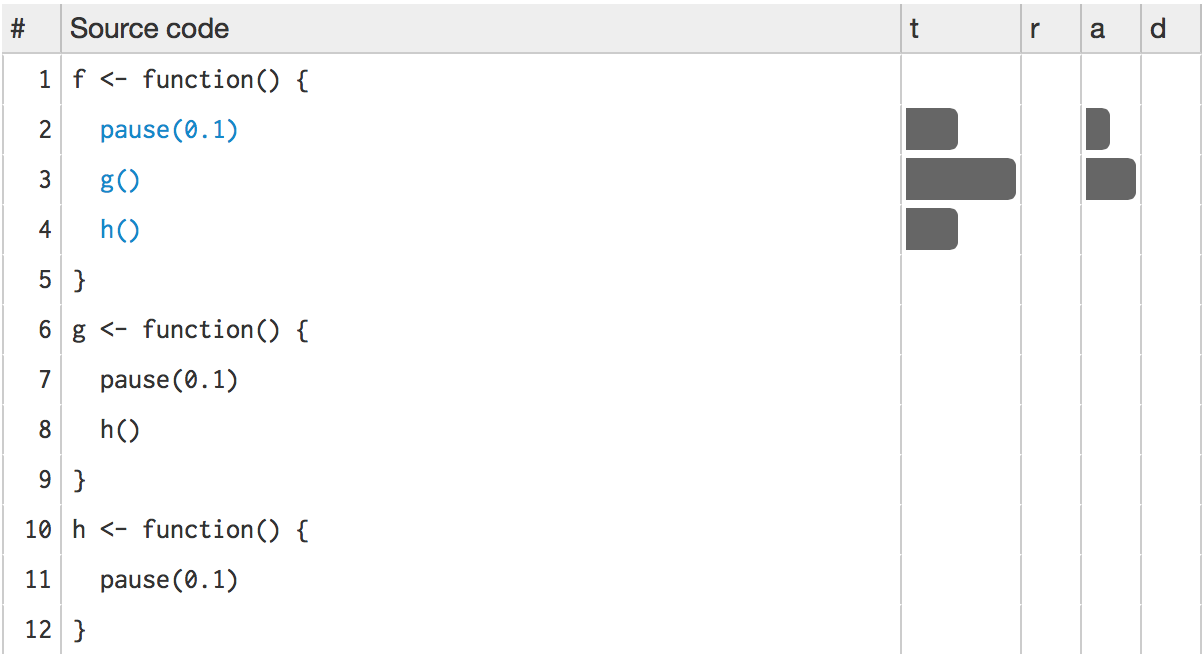
\includegraphics[width=4.35in]{screenshots/profiling-lineprof-f.png}

The \texttt{t} column visualises how much time is spent on each line.
(You'll learn about the other columns in
\hyperref[memory-profiling]{memory profiling}.) While not precise, it
allows you to spot bottlenecks, and you can get precise numbers by
hovering over each bar. This shows that twice as much time is spent on
\texttt{g()} as on \texttt{h()}, so it would make sense to drill down
into \texttt{g()} for more details. To do so, click \texttt{g()}:

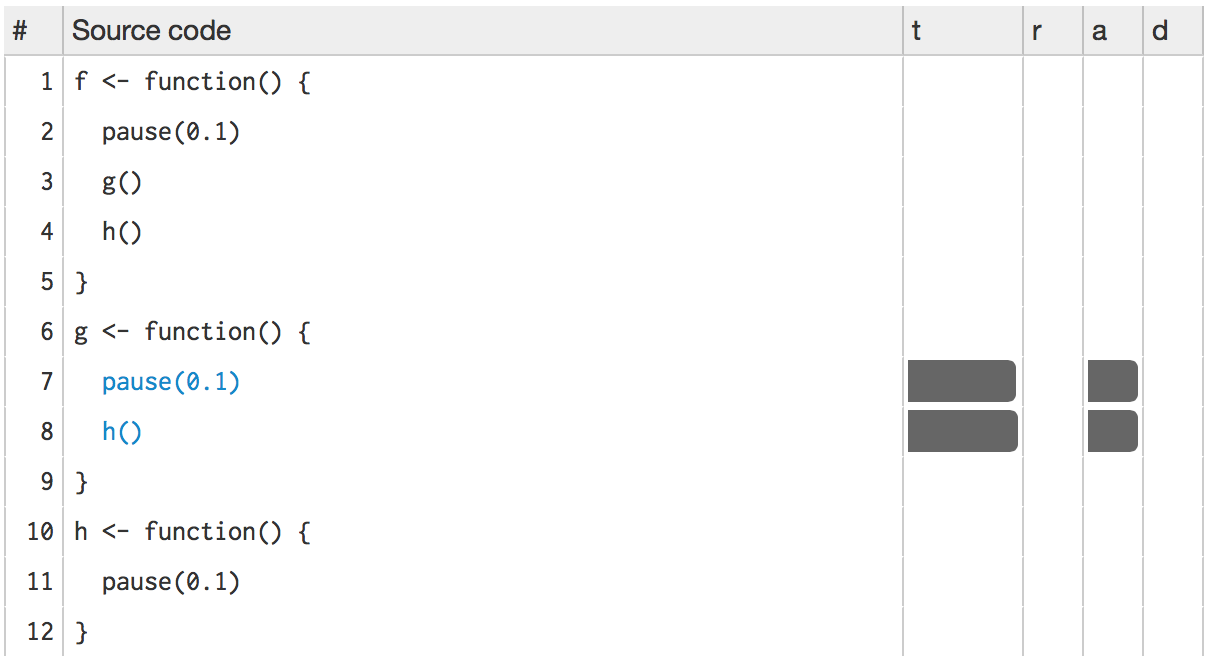
\includegraphics[width=4.35in]{screenshots/profiling-lineprof-g.png}

Then \texttt{h()}:

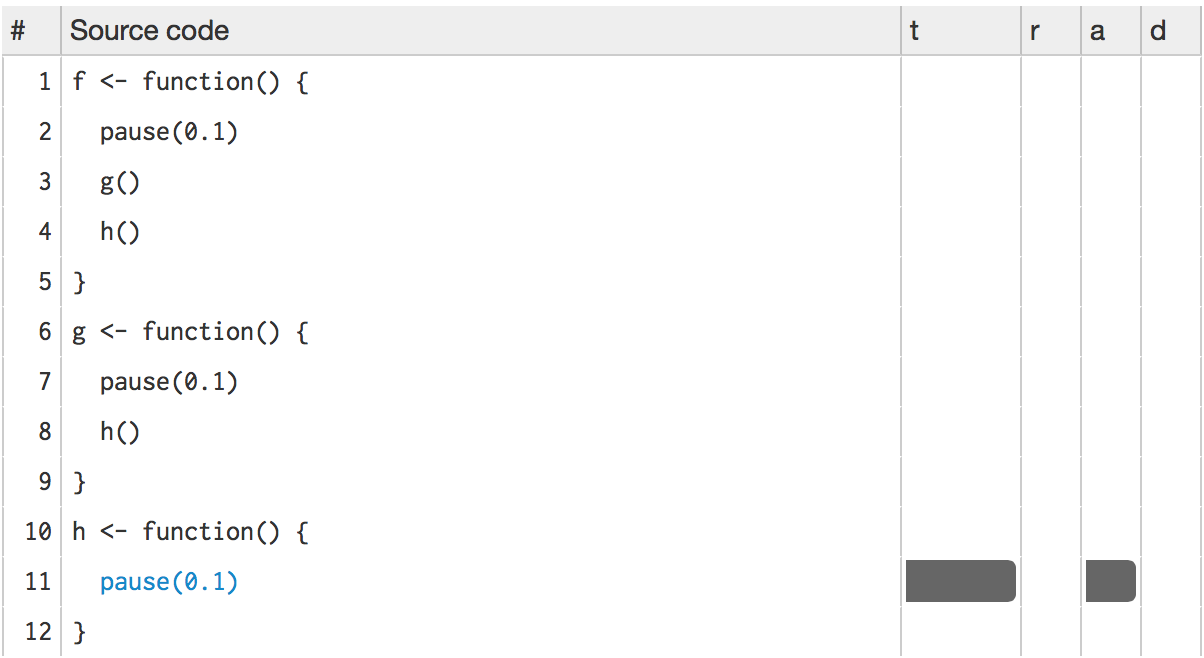
\includegraphics[width=4.35in]{screenshots/profiling-lineprof-h.png}

This technique should allow you to quickly identify the major
bottlenecks in your code.

\subsection{Limitations}

There are some other limitations to profiling:

\begin{itemize}
\item
  Profiling does not extend to C code. You can see if your R code calls
  C/C++ code but not what functions are called inside of your C/C++
  code. Unfortunately, tools for profiling compiled code are beyond the
  scope of this book (i.e., I have no idea how to do it).
\item
  Similarly, you can't see what's going on inside primitive functions or
  byte code compiled code.
\item
  If you're doing a lot of functional programming with anonymous
  functions, it can be hard to figure out exactly which function is
  being called. The easiest way to work around this is to name your
  functions.
\item
  Lazy evaluation means that arguments are often evaluated inside
  another function. For example, in the following code, profiling would
  make it seem like \texttt{i()} was called by \texttt{j()} because the
  argument isn't evaluated until it's needed by \texttt{j()}.

\begin{Shaded}
\begin{Highlighting}[]
\NormalTok{i <-}\StringTok{ }\NormalTok{function() \{}
  \KeywordTok{pause}\NormalTok{(}\FloatTok{0.1}\NormalTok{)}
  \DecValTok{10}
\NormalTok{\}}
\NormalTok{j <-}\StringTok{ }\NormalTok{function(x) \{}
  \NormalTok{x +}\StringTok{ }\DecValTok{10}
\NormalTok{\}}
\KeywordTok{j}\NormalTok{(}\KeywordTok{i}\NormalTok{())}
\end{Highlighting}
\end{Shaded}

  If this is confusing, you can create temporary variables to force
  computation to happen earlier.
\end{itemize}

\hyperdef{}{improve-perf}{\section{Improving
performance}\label{improve-perf}}

\begin{quote}
``We should forget about small efficiencies, say about 97\% of the time:
premature optimization is the root of all evil. Yet we should not pass
up our opportunities in that critical 3\%. A good programmer will not be
lulled into complacency by such reasoning, he will be wise to look
carefully at the critical code; but only after that code has been
identified.''

--- Donald Knuth.
\end{quote}

Once you've used profiling to identify a bottleneck, you need to make it
faster. The following sections introduce you to a number of techniques
that I've found broadly useful: \index{improving performance}
\index{performance!improving}

\begin{enumerate}
\def\labelenumi{\arabic{enumi}.}
\itemsep1pt\parskip0pt\parsep0pt
\item
  Look for existing solutions.
\item
  Do less work.
\item
  Vectorise.
\item
  Parallelise.
\item
  Avoid copies.
\item
  Byte-code compile.
\end{enumerate}

A final technique is to rewrite in a faster language, like C++. That's a
big topic and is covered in \hyperref[rcpp]{Rcpp}.

Before we get into specific techniques, I'll first describe a general
strategy and organisational style that's useful when working on
performance.

\hyperdef{}{code-organisation}{\section{Code
organisation}\label{code-organisation}}

There are two traps that are easy to fall into when trying to make your
code faster:

\begin{enumerate}
\def\labelenumi{\arabic{enumi}.}
\itemsep1pt\parskip0pt\parsep0pt
\item
  Writing faster but incorrect code.
\item
  Writing code that you think is faster, but is actually no better.
\end{enumerate}

The strategy outlined below will help you avoid these pitfalls.
\index{improving performance!strategy}

When tackling a bottleneck, you're likely to come up with multiple
approaches. Write a function for each approach, encapsulating all
relevant behaviour. This makes it easier to check that each approach
returns the correct result and to time how long it takes to run. To
demonstrate the strategy, I'll compare two approaches for computing the
mean:

\begin{Shaded}
\begin{Highlighting}[]
\NormalTok{mean1 <-}\StringTok{ }\NormalTok{function(x) }\KeywordTok{mean}\NormalTok{(x)}
\NormalTok{mean2 <-}\StringTok{ }\NormalTok{function(x) }\KeywordTok{sum}\NormalTok{(x) /}\StringTok{ }\KeywordTok{length}\NormalTok{(x)}
\end{Highlighting}
\end{Shaded}

I recommend that you keep a record of everything you try, even the
failures. If a similar problem occurs in the future, it'll be useful to
see everything you've tried. To do this I often use R Markdown, which
makes it easy to intermingle code with detailed comments and notes.

Next, generate a representative test case. The case should be big enough
to capture the essence of your problem but small enough that it takes
only a few seconds to run. You don't want it to take too long because
you'll need to run the test case many times to compare approaches. On
the other hand, you don't want the case to be too small because then
results might not scale up to the real problem.

Use this test case to quickly check that all variants return the same
result. An easy way to do so is with \texttt{stopifnot()} and
\texttt{all.equal()}. For real problems with fewer possible outputs, you
may need more tests to make sure that an approach doesn't accidentally
return the correct answer. That's unlikely for the mean.
\indexc{stopifnot()}

\begin{Shaded}
\begin{Highlighting}[]
\NormalTok{x <-}\StringTok{ }\KeywordTok{runif}\NormalTok{(}\DecValTok{100}\NormalTok{)}
\KeywordTok{stopifnot}\NormalTok{(}\KeywordTok{all.equal}\NormalTok{(}\KeywordTok{mean1}\NormalTok{(x), }\KeywordTok{mean2}\NormalTok{(x)))}
\end{Highlighting}
\end{Shaded}

Finally, use the \texttt{microbenchmark} package to compare how long
each variation takes to run. For bigger problems, reduce the
\texttt{times} parameter so that it only takes a couple of seconds to
run. Focus on the median time, and use the upper and lower quartiles to
gauge the variability of the measurement. \indexc{microbenchmark()}

\begin{Shaded}
\begin{Highlighting}[]
\KeywordTok{microbenchmark}\NormalTok{(}
  \KeywordTok{mean1}\NormalTok{(x),}
  \KeywordTok{mean2}\NormalTok{(x)}
\NormalTok{)}
\CommentTok{#> Unit: nanoseconds}
\CommentTok{#>      expr   min    lq median    uq    max neval}
\CommentTok{#>  mean1(x) 5,680 6,080  6,250 6,490 38,500   100}
\CommentTok{#>  mean2(x)   763 1,010  1,220 1,380 17,300   100}
\end{Highlighting}
\end{Shaded}

(You might be surprised by the results: \texttt{mean(x)} is considerably
slower than \texttt{sum(x) / length(x)}. This is because, among other
reasons, \texttt{mean(x)} makes two passes over the vector to be more
numerically accurate.)

Before you start experimenting, you should have a target speed that
defines when the bottleneck is no longer a problem. Setting such a goal
is important because you don't want to spend valuable time
over-optimising your code.

If you'd like to see this strategy in action, I've used it a few times
on stackoverflow:

\begin{itemize}
\itemsep1pt\parskip0pt\parsep0pt
\item
  \url{http://stackoverflow.com/questions/22515525\#22518603}
\item
  \url{http://stackoverflow.com/questions/22515175\#22515856}
\item
  \url{http://stackoverflow.com/questions/3476015\#22511936}
\end{itemize}

\hyperdef{}{already-solved}{\section{Has someone already solved the
problem?}\label{already-solved}}

Once you've organised your code and captured all the variations you can
think of, it's natural to see what others have done. You are part of a
large community, and it's quite possible that someone has already
tackled the same problem. If your bottleneck is a function in a package,
it's worth looking at other packages that do the same thing. Two good
places to start are:

\begin{itemize}
\item
  \href{http://cran.rstudio.com/web/views/}{CRAN task views}. If there's
  a CRAN task view related to your problem domain, it's worth looking at
  the packages listed there.
\item
  Reverse dependencies of Rcpp, as listed on its
  \href{http://cran.r-project.org/web/packages/Rcpp}{CRAN page}. Since
  these packages use C++, it's possible to find a solution to your
  bottleneck written in a higher performance language.
\end{itemize}

Otherwise, the challenge is describing your bottleneck in a way that
helps you find related problems and solutions. Knowing the name of the
problem or its synonyms will make this search much easier. But because
you don't know what it's called, it's hard to search for it! By reading
broadly about statistics and algorithms, you can build up your own
knowledge base over time. Alternatively, ask others. Talk to your
colleagues and brainstorm some possible names, then search on Google and
stackoverflow. It's often helpful to restrict your search to R related
pages. For Google, try \href{http://www.rseek.org/}{rseek}. For
stackoverflow, restrict your search by including the R tag,
\texttt{{[}R{]}}, in your search. \index{searching}

As discussed above, record all solutions that you find, not just those
that immediately appear to be faster. Some solutions might be initially
slower, but because they are easier to optimise they end up being
faster. You may also be able to combine the fastest parts from different
approaches. If you've found a solution that's fast enough,
congratulations! If appropriate, you may want to share your solution
with the R community. Otherwise, read on.

\subsection{Exercises}

\begin{enumerate}
\def\labelenumi{\arabic{enumi}.}
\item
  What are faster alternatives to \texttt{lm}? Which are specifically
  designed to work with larger datasets?
\item
  What package implements a version of \texttt{match()} that's faster
  for repeated lookups? How much faster is it?
\item
  List four functions (not just those in base R) that convert a string
  into a date time object. What are their strengths and weaknesses?
\item
  How many different ways can you compute a 1d density estimate in R?
\item
  Which packages provide the ability to compute a rolling mean?
\item
  What are the alternatives to \texttt{optim()}?
\end{enumerate}

\hyperdef{}{be-lazy}{\section{Do as little as possible}\label{be-lazy}}

The easiest way to make a function faster is to let it do less work. One
way to do that is use a function tailored to a more specific type of
input or ouput, or a more specific problem. For example:

\begin{itemize}
\item
  \texttt{rowSums()}, \texttt{colSums()}, \texttt{rowMeans()}, and
  \texttt{colMeans()} are faster than equivalent invocations that use
  \texttt{apply()} because they are vectorised (the topic of the next
  section).
\item
  \texttt{vapply()} is faster than \texttt{sapply()} because it
  pre-specifies the output type.
\item
  If you want to see if a vector contains a single value,
  \texttt{any(x == 10)} is much faster than \texttt{10 \%in\% x}. This
  is because testing equality is simpler than testing inclusion in a
  set.
\end{itemize}

Having this knowledge at your fingertips requires knowing that
alternative functions exist: you need to have a good vocabulary. Start
with \hyperref[vocabulary]{the basics}, and expand your vocab by
regularly reading R code. Good places to read code are the
\href{https://stat.ethz.ch/mailman/listinfo/r-help}{R-help mailing list}
and \href{http://stackoverflow.com/questions/tagged/r}{stackoverflow}.

Some functions coerce their inputs into a specific type. If your input
is not the right type, the function has to do extra work. Instead, look
for a function that works with your data as it is, or consider changing
the way you store your data. The most common example of this problem is
using \texttt{apply()} on a data frame. \texttt{apply()} always turns
its input into a matrix. Not only is this error prone (because a data
frame is more general than a matrix), it is also slower.

Other functions will do less work if you give them more information
about the problem. It's always worthwhile to carefully read the
documentation and experiment with different arguments. Some examples
that I've discovered in the past include:

\begin{itemize}
\item
  \texttt{read.csv()}: specify known column types with
  \texttt{colClasses}.
\item
  \texttt{factor()}: specify known levels with \texttt{levels}.
\item
  \texttt{cut()}: don't generate labels with \texttt{labels = FALSE} if
  you don't need them, or, even better, use \texttt{findInterval()} as
  mentioned in the ``see also'' section of the documentation.
\item
  \texttt{unlist(x, use.names = FALSE)} is much faster than
  \texttt{unlist(x)}.
\item
  \texttt{interaction()}: if you only need combinations that exist in
  the data, use \texttt{drop = TRUE}.
\end{itemize}

Sometimes you can make a function faster by avoiding method dispatch. As
we saw in (\hyperref[extreme-dynamism]{Extreme dynamism}), method
dispatch in R can be costly. If you're calling a method in a tight loop,
you can avoid some of the costs by doing the method lookup only once:
\index{methods!cost of dispatch, avoiding}

\begin{itemize}
\item
  For S3, you can do this by calling \texttt{generic.class()} instead of
  \texttt{generic()}.
\item
  For S4, you can do this by using \texttt{findMethod()} to find the
  method, saving it to a variable, and then calling that function.
\end{itemize}

For example, calling \texttt{mean.default()} quite a bit faster than
calling \texttt{mean()} for small vectors:

\begin{Shaded}
\begin{Highlighting}[]
\NormalTok{x <-}\StringTok{ }\KeywordTok{runif}\NormalTok{(}\FloatTok{1e2}\NormalTok{)}

\KeywordTok{microbenchmark}\NormalTok{(}
  \KeywordTok{mean}\NormalTok{(x),}
  \KeywordTok{mean.default}\NormalTok{(x)}
\NormalTok{)}
\CommentTok{#> Unit: microseconds}
\CommentTok{#>             expr  min   lq median   uq  max neval}
\CommentTok{#>          mean(x) 4.86 5.09   5.25 5.45 47.1   100}
\CommentTok{#>  mean.default(x) 1.38 1.56   1.64 1.76 32.7   100}
\end{Highlighting}
\end{Shaded}

This optimisation is a little risky. While \texttt{mean.default()} is
almost twice as fast, it'll fail in surprising ways if \texttt{x} is not
a numeric vector. You should only use it if you know for sure what
\texttt{x} is.

Knowing that you're dealing with a specific type of input can be another
way to write faster code. For example, \texttt{as.data.frame()} is quite
slow because it coerces each element into a data frame and then
\texttt{rbind()}s them together. If you have a named list with vectors
of equal length, you can directly transform it into a data frame. In
this case, if you're able to make strong assumptions about your input,
you can write a method that's about 20x faster than the default.

\begin{Shaded}
\begin{Highlighting}[]
\NormalTok{quickdf <-}\StringTok{ }\NormalTok{function(l) \{}
  \KeywordTok{class}\NormalTok{(l) <-}\StringTok{ "data.frame"}
  \KeywordTok{attr}\NormalTok{(l, }\StringTok{"row.names"}\NormalTok{) <-}\StringTok{ }\KeywordTok{.set_row_names}\NormalTok{(}\KeywordTok{length}\NormalTok{(l[[}\DecValTok{1}\NormalTok{]]))}
  \NormalTok{l}
\NormalTok{\}}

\NormalTok{l <-}\StringTok{ }\KeywordTok{lapply}\NormalTok{(}\DecValTok{1}\NormalTok{:}\DecValTok{26}\NormalTok{, function(i) }\KeywordTok{runif}\NormalTok{(}\FloatTok{1e3}\NormalTok{))}
\KeywordTok{names}\NormalTok{(l) <-}\StringTok{ }\NormalTok{letters}

\KeywordTok{microbenchmark}\NormalTok{(}
  \DataTypeTok{quick_df      =} \KeywordTok{quickdf}\NormalTok{(l),}
  \DataTypeTok{as.data.frame =} \KeywordTok{as.data.frame}\NormalTok{(l)}
\NormalTok{)}
\CommentTok{#> Unit: microseconds}
\CommentTok{#>           expr     min      lq  median      uq   max neval}
\CommentTok{#>       quick_df    14.4    16.1    21.1    28.3    81   100}
\CommentTok{#>  as.data.frame 1,480.0 1,530.0 1,600.0 1,870.0 4,300   100}
\end{Highlighting}
\end{Shaded}

Again, note the trade-off. This method is fast because it's dangerous.
If you give it bad inputs, you'll get a corrupt data frame:

\begin{Shaded}
\begin{Highlighting}[]
\KeywordTok{quickdf}\NormalTok{(}\KeywordTok{list}\NormalTok{(}\DataTypeTok{x =} \DecValTok{1}\NormalTok{, }\DataTypeTok{y =} \DecValTok{1}\NormalTok{:}\DecValTok{2}\NormalTok{))}
\CommentTok{#> Warning in format.data.frame(x, digits = digits, na.encode =}
\CommentTok{#> FALSE): corrupt data frame: columns will be truncated or}
\CommentTok{#> padded with NAs}
\CommentTok{#>   x y}
\CommentTok{#> 1 1 1}
\end{Highlighting}
\end{Shaded}

To come up with this minimal method, I carefully read through and then
rewrote the source code for \texttt{as.data.frame.list()} and
\texttt{data.frame()}. I made many small changes, each time checking
that I hadn't broken existing behaviour. After several hours work, I was
able to isolate the minimal code shown above. This is a very useful
technique. Most base R functions are written for flexibility and
functionality, not performance. Thus, rewriting for your specific need
can often yield substantial improvements. To do this, you'll need to
read the source code. It can be complex and confusing, but don't give
up!

The following example shows a progressive simplification of the
\texttt{diff()} function if you only want computing differences between
adjacent values. At each step, I replace one argument with a specific
case, and then check to see that the function still works. The initial
function is long and complicated, but by restricting the arguments I not
only make it around twice as fast, I also make it easier to understand.

First, I take the code of \texttt{diff()} and reformat it to my style:
\indexc{diff()}

\begin{Shaded}
\begin{Highlighting}[]
\NormalTok{diff1 <-}\StringTok{ }\NormalTok{function (x, }\DataTypeTok{lag =} \NormalTok{1L, }\DataTypeTok{differences =} \NormalTok{1L) \{}
  \NormalTok{ismat <-}\StringTok{ }\KeywordTok{is.matrix}\NormalTok{(x)}
  \NormalTok{xlen <-}\StringTok{ }\NormalTok{if (ismat) }\KeywordTok{dim}\NormalTok{(x)[1L] else }\KeywordTok{length}\NormalTok{(x)}
  \NormalTok{if (}\KeywordTok{length}\NormalTok{(lag) >}\StringTok{ }\NormalTok{1L ||}\StringTok{ }\KeywordTok{length}\NormalTok{(differences) >}\StringTok{ }\NormalTok{1L ||}\StringTok{ }
\StringTok{      }\NormalTok{lag <}\StringTok{ }\NormalTok{1L ||}\StringTok{ }\NormalTok{differences <}\StringTok{ }\NormalTok{1L)}
    \KeywordTok{stop}\NormalTok{(}\StringTok{"'lag' and 'differences' must be integers >= 1"}\NormalTok{)}

  \NormalTok{if (lag *}\StringTok{ }\NormalTok{differences >=}\StringTok{ }\NormalTok{xlen) \{}
    \KeywordTok{return}\NormalTok{(x[0L])}
  \NormalTok{\}}

  \NormalTok{r <-}\StringTok{ }\KeywordTok{unclass}\NormalTok{(x)}
  \NormalTok{i1 <-}\StringTok{ }\NormalTok{-}\KeywordTok{seq_len}\NormalTok{(lag)}
  \NormalTok{if (ismat) \{}
    \NormalTok{for (i in }\KeywordTok{seq_len}\NormalTok{(differences)) \{}
      \NormalTok{r <-}\StringTok{ }\NormalTok{r[i1, , drop =}\StringTok{ }\OtherTok{FALSE}\NormalTok{] -}\StringTok{ }
\StringTok{        }\NormalTok{r[-}\KeywordTok{nrow}\NormalTok{(r):-(}\KeywordTok{nrow}\NormalTok{(r) -}\StringTok{ }\NormalTok{lag +}\StringTok{ }\NormalTok{1L), , drop =}\StringTok{ }\OtherTok{FALSE}\NormalTok{]}
    \NormalTok{\}}
  \NormalTok{\} else \{}
    \NormalTok{for (i in }\KeywordTok{seq_len}\NormalTok{(differences)) \{}
      \NormalTok{r <-}\StringTok{ }\NormalTok{r[i1] -}\StringTok{ }\NormalTok{r[-}\KeywordTok{length}\NormalTok{(r):-(}\KeywordTok{length}\NormalTok{(r) -}\StringTok{ }\NormalTok{lag +}\StringTok{ }\NormalTok{1L)]}
    \NormalTok{\}}
  \NormalTok{\}}
  \KeywordTok{class}\NormalTok{(r) <-}\StringTok{ }\KeywordTok{oldClass}\NormalTok{(x)}
  \NormalTok{r}
\NormalTok{\}}
\end{Highlighting}
\end{Shaded}

Next, I assume vector input. This allows me to remove the
\texttt{is.matrix()} test and the method that uses matrix subsetting.

\begin{Shaded}
\begin{Highlighting}[]
\NormalTok{diff2 <-}\StringTok{ }\NormalTok{function (x, }\DataTypeTok{lag =} \NormalTok{1L, }\DataTypeTok{differences =} \NormalTok{1L) \{}
  \NormalTok{xlen <-}\StringTok{ }\KeywordTok{length}\NormalTok{(x)}
  \NormalTok{if (}\KeywordTok{length}\NormalTok{(lag) >}\StringTok{ }\NormalTok{1L ||}\StringTok{ }\KeywordTok{length}\NormalTok{(differences) >}\StringTok{ }\NormalTok{1L ||}\StringTok{ }
\StringTok{      }\NormalTok{lag <}\StringTok{ }\NormalTok{1L ||}\StringTok{ }\NormalTok{differences <}\StringTok{ }\NormalTok{1L)}
    \KeywordTok{stop}\NormalTok{(}\StringTok{"'lag' and 'differences' must be integers >= 1"}\NormalTok{)}

  \NormalTok{if (lag *}\StringTok{ }\NormalTok{differences >=}\StringTok{ }\NormalTok{xlen) \{}
    \KeywordTok{return}\NormalTok{(x[0L])}
  \NormalTok{\}}

  \NormalTok{i1 <-}\StringTok{ }\NormalTok{-}\KeywordTok{seq_len}\NormalTok{(lag)}
  \NormalTok{for (i in }\KeywordTok{seq_len}\NormalTok{(differences)) \{}
    \NormalTok{x <-}\StringTok{ }\NormalTok{x[i1] -}\StringTok{ }\NormalTok{x[-}\KeywordTok{length}\NormalTok{(x):-(}\KeywordTok{length}\NormalTok{(x) -}\StringTok{ }\NormalTok{lag +}\StringTok{ }\NormalTok{1L)]}
  \NormalTok{\}}
  \NormalTok{x}
\NormalTok{\}}
\KeywordTok{diff2}\NormalTok{(}\KeywordTok{cumsum}\NormalTok{(}\DecValTok{0}\NormalTok{:}\DecValTok{10}\NormalTok{))}
\CommentTok{#>  [1]  1  2  3  4  5  6  7  8  9 10}
\end{Highlighting}
\end{Shaded}

I now assume that \texttt{difference = 1L}. This simplifies input
checking and eliminates the for loop:

\begin{Shaded}
\begin{Highlighting}[]
\NormalTok{diff3 <-}\StringTok{ }\NormalTok{function (x, }\DataTypeTok{lag =} \NormalTok{1L) \{}
  \NormalTok{xlen <-}\StringTok{ }\KeywordTok{length}\NormalTok{(x)}
  \NormalTok{if (}\KeywordTok{length}\NormalTok{(lag) >}\StringTok{ }\NormalTok{1L ||}\StringTok{ }\NormalTok{lag <}\StringTok{ }\NormalTok{1L)}
    \KeywordTok{stop}\NormalTok{(}\StringTok{"'lag' must be integer >= 1"}\NormalTok{)}

  \NormalTok{if (lag >=}\StringTok{ }\NormalTok{xlen) \{}
    \KeywordTok{return}\NormalTok{(x[0L])}
  \NormalTok{\}}

  \NormalTok{i1 <-}\StringTok{ }\NormalTok{-}\KeywordTok{seq_len}\NormalTok{(lag)}
  \NormalTok{x[i1] -}\StringTok{ }\NormalTok{x[-}\KeywordTok{length}\NormalTok{(x):-(}\KeywordTok{length}\NormalTok{(x) -}\StringTok{ }\NormalTok{lag +}\StringTok{ }\NormalTok{1L)]}
\NormalTok{\}}
\KeywordTok{diff3}\NormalTok{(}\KeywordTok{cumsum}\NormalTok{(}\DecValTok{0}\NormalTok{:}\DecValTok{10}\NormalTok{))}
\CommentTok{#>  [1]  1  2  3  4  5  6  7  8  9 10}
\end{Highlighting}
\end{Shaded}

Finally I assume \texttt{lag = 1L}. This eliminates input checking and
simplifies subsetting.

\begin{Shaded}
\begin{Highlighting}[]
\NormalTok{diff4 <-}\StringTok{ }\NormalTok{function (x) \{}
  \NormalTok{xlen <-}\StringTok{ }\KeywordTok{length}\NormalTok{(x)}
  \NormalTok{if (xlen <=}\StringTok{ }\DecValTok{1}\NormalTok{) }\KeywordTok{return}\NormalTok{(x[0L])}

  \NormalTok{x[-}\DecValTok{1}\NormalTok{] -}\StringTok{ }\NormalTok{x[-xlen]}
\NormalTok{\}}
\KeywordTok{diff4}\NormalTok{(}\KeywordTok{cumsum}\NormalTok{(}\DecValTok{0}\NormalTok{:}\DecValTok{10}\NormalTok{))}
\CommentTok{#>  [1]  1  2  3  4  5  6  7  8  9 10}
\end{Highlighting}
\end{Shaded}

Now \texttt{diff4()} is both considerably simpler and considerably
faster than \texttt{diff1()}:

\begin{Shaded}
\begin{Highlighting}[]
\NormalTok{x <-}\StringTok{ }\KeywordTok{runif}\NormalTok{(}\DecValTok{100}\NormalTok{)}
\KeywordTok{microbenchmark}\NormalTok{(}
  \KeywordTok{diff1}\NormalTok{(x),}
  \KeywordTok{diff2}\NormalTok{(x),}
  \KeywordTok{diff3}\NormalTok{(x),}
  \KeywordTok{diff4}\NormalTok{(x)}
\NormalTok{)}
\CommentTok{#> Unit: microseconds}
\CommentTok{#>      expr   min    lq median    uq  max neval}
\CommentTok{#>  diff1(x) 11.70 14.00  14.60 15.10 43.7   100}
\CommentTok{#>  diff2(x) 10.20 12.60  12.80 13.10 69.4   100}
\CommentTok{#>  diff3(x)  9.03 11.00  11.30 11.70 29.4   100}
\CommentTok{#>  diff4(x)  7.12  9.38   9.56  9.82 16.8   100}
\end{Highlighting}
\end{Shaded}

You'll be able to make \texttt{diff()} even faster for this special case
once you've read \hyperref[rcpp]{Rcpp}.

A final example of doing less work is to use simpler data structures.
For example, when working with rows from a data frame, it's often faster
to work with row indices than data frames. For instance, if you wanted
to compute a bootstrap estimate of the correlation between two columns
in a data frame, there are two basic approaches: you can either work
with the whole data frame or with the individual vectors. The following
example shows that working with vectors is about twice as fast.
\index{bootstrapping}

\begin{Shaded}
\begin{Highlighting}[]
\NormalTok{sample_rows <-}\StringTok{ }\NormalTok{function(df, i) }\KeywordTok{sample.int}\NormalTok{(}\KeywordTok{nrow}\NormalTok{(df), i, }
  \DataTypeTok{replace =} \OtherTok{TRUE}\NormalTok{)}

\CommentTok{# Generate a new data frame containing randomly selected rows}
\NormalTok{boot_cor1 <-}\StringTok{ }\NormalTok{function(df, i) \{}
  \NormalTok{sub <-}\StringTok{ }\NormalTok{df[}\KeywordTok{sample_rows}\NormalTok{(df, i), , drop =}\StringTok{ }\OtherTok{FALSE}\NormalTok{]}
  \KeywordTok{cor}\NormalTok{(sub$x, sub$y)}
\NormalTok{\}}

\CommentTok{# Generate new vectors from random rows}
\NormalTok{boot_cor2 <-}\StringTok{ }\NormalTok{function(df, i ) \{}
  \NormalTok{idx <-}\StringTok{ }\KeywordTok{sample_rows}\NormalTok{(df, i)}
  \KeywordTok{cor}\NormalTok{(df$x[idx], df$y[idx])}
\NormalTok{\}}

\NormalTok{df <-}\StringTok{ }\KeywordTok{data.frame}\NormalTok{(}\DataTypeTok{x =} \KeywordTok{runif}\NormalTok{(}\DecValTok{100}\NormalTok{), }\DataTypeTok{y =} \KeywordTok{runif}\NormalTok{(}\DecValTok{100}\NormalTok{))}
\KeywordTok{microbenchmark}\NormalTok{(}
  \KeywordTok{boot_cor1}\NormalTok{(df, }\DecValTok{10}\NormalTok{),}
  \KeywordTok{boot_cor2}\NormalTok{(df, }\DecValTok{10}\NormalTok{)}
\NormalTok{)}
\CommentTok{#> Unit: microseconds}
\CommentTok{#>               expr   min    lq median    uq max neval}
\CommentTok{#>  boot_cor1(df, 10) 129.0 136.0  141.0 148.0 752   100}
\CommentTok{#>  boot_cor2(df, 10)  76.5  79.5   82.1  87.3 130   100}
\end{Highlighting}
\end{Shaded}

\subsection{Exercises}

\begin{enumerate}
\def\labelenumi{\arabic{enumi}.}
\item
  How do the results change if you compare \texttt{mean()} and
  \texttt{mean.default()} on 10,000 observations, rather than on 100?
\item
  The following code provides an alternative implementation of
  \texttt{rowSums()}. Why is it faster for this input?

\begin{Shaded}
\begin{Highlighting}[]
\NormalTok{rowSums2 <-}\StringTok{ }\NormalTok{function(df) \{}
  \NormalTok{out <-}\StringTok{ }\NormalTok{df[[1L]]}
  \NormalTok{if (}\KeywordTok{ncol}\NormalTok{(df) ==}\StringTok{ }\DecValTok{1}\NormalTok{) }\KeywordTok{return}\NormalTok{(out)}

  \NormalTok{for (i in }\DecValTok{2}\NormalTok{:}\KeywordTok{ncol}\NormalTok{(df)) \{}
    \NormalTok{out <-}\StringTok{ }\NormalTok{out +}\StringTok{ }\NormalTok{df[[i]]}
  \NormalTok{\}}
  \NormalTok{out}
\NormalTok{\}}

\NormalTok{df <-}\StringTok{ }\KeywordTok{as.data.frame}\NormalTok{(}
  \KeywordTok{replicate}\NormalTok{(}\FloatTok{1e3}\NormalTok{, }\KeywordTok{sample}\NormalTok{(}\DecValTok{100}\NormalTok{, }\FloatTok{1e4}\NormalTok{, }\DataTypeTok{replace =} \OtherTok{TRUE}\NormalTok{))}
\NormalTok{)}
\KeywordTok{system.time}\NormalTok{(}\KeywordTok{rowSums}\NormalTok{(df))}
\CommentTok{#>    user  system elapsed }
\CommentTok{#>   0.062   0.003   0.066}
\KeywordTok{system.time}\NormalTok{(}\KeywordTok{rowSums2}\NormalTok{(df))}
\CommentTok{#>    user  system elapsed }
\CommentTok{#>   0.056   0.008   0.063}
\end{Highlighting}
\end{Shaded}
\item
  What's the difference between \texttt{rowSums()} and
  \texttt{.rowSums()}?
\item
  Make a faster version of \texttt{chisq.test()} that only computes the
  chi-square test statistic when the input is two numeric vectors with
  no missing values. You can try simplifying \texttt{chisq.test()} or by
  coding from the
  \href{http://en.wikipedia.org/wiki/Pearson\%27s_chi-squared_test}{mathematical
  definition}.
\item
  Can you make a faster version of \texttt{table()} for the case of an
  input of two integer vectors with no missing values? Can you use it to
  speed up your chi-square test?
\item
  Imagine you want to compute the bootstrap distribution of a sample
  correlation using \texttt{cor\_df()} and the data in the example
  below. Given that you want to run this many times, how can you make
  this code faster? (Hint: the function has three components that you
  can speed up.)

\begin{Shaded}
\begin{Highlighting}[]
\NormalTok{n <-}\StringTok{ }\FloatTok{1e6}
\NormalTok{df <-}\StringTok{ }\KeywordTok{data.frame}\NormalTok{(}\DataTypeTok{a =} \KeywordTok{rnorm}\NormalTok{(n), }\DataTypeTok{b =} \KeywordTok{rnorm}\NormalTok{(n))}

\NormalTok{cor_df <-}\StringTok{ }\NormalTok{function(i) \{}
  \NormalTok{i <-}\StringTok{ }\KeywordTok{sample}\NormalTok{(}\KeywordTok{seq}\NormalTok{(n), n *}\StringTok{ }\FloatTok{0.01}\NormalTok{)}
  \KeywordTok{cor}\NormalTok{(q[i, , }\DataTypeTok{drop =} \OtherTok{FALSE}\NormalTok{])[}\DecValTok{2}\NormalTok{,}\DecValTok{1}\NormalTok{]}
\NormalTok{\}}
\end{Highlighting}
\end{Shaded}

  Is there a way to vectorise this procedure?
\end{enumerate}

\hyperdef{}{vectorise}{\section{Vectorise}\label{vectorise}}

If you've used R for any length of time, you've probably heard the
admonishment to ``vectorise your code''. But what does that actually
mean? Vectorising your code is not just about avoiding for loops,
although that's often a step. Vectorising is about taking a ``whole
object'' approach to a problem, thinking about vectors, not scalars.
There are two key attributes of a vectorised function:
\index{vectorising code}

\begin{itemize}
\item
  It makes many problems simpler. Instead of having to think about the
  components of a vector, you only think about entire vectors.
\item
  The loops in a vectorised function are written in C instead of R.
  Loops in C are much faster because they have much less overhead.
\end{itemize}

\hyperref[functionals]{Functionals} stressed the importance of
vectorised code as a higher level abstraction. Vectorisation is also
important for writing fast R code. This doesn't mean simply using
\texttt{apply()} or \texttt{lapply()}, or even \texttt{Vectorise()}.
Those functions improve the interface of a function, but don't
fundamentally change performance. Using vectorisation for performance
means finding the existing R function that is implemented in C and most
closely applies to your problem.

Vectorised functions that apply to many common performance bottlenecks
include:

\begin{itemize}
\item
  \texttt{rowSums()}, \texttt{colSums()}, \texttt{rowMeans()}, and
  \texttt{colMeans()}. These vectorised matrix functions will always be
  faster than using \texttt{apply()}. You can sometimes use these
  functions to build other vectorised functions.

\begin{Shaded}
\begin{Highlighting}[]
\NormalTok{rowAny <-}\StringTok{ }\NormalTok{function(x) }\KeywordTok{rowSums}\NormalTok{(x) >}\StringTok{ }\DecValTok{0}
\NormalTok{rowAll <-}\StringTok{ }\NormalTok{function(x) }\KeywordTok{rowSums}\NormalTok{(x) ==}\StringTok{ }\KeywordTok{ncol}\NormalTok{(x)}
\end{Highlighting}
\end{Shaded}
\item
  Vectorised subsetting can lead to big improvements in speed. Remember
  the techniques behind lookup tables (\hyperref[lookup-tables]{lookup
  tables}) and matching and merging by hand
  (\hyperref[matching-merging]{matching and merging by hand}). Also
  remember that you can use subsetting assignment to replace multiple
  values in a single step. If \texttt{x} is a vector, matrix or data
  frame then \texttt{x{[}is.na(x){]} \textless{}- 0} will replace all
  missing values with 0.
\item
  If you're extracting or replacing values in scattered locations in a
  matrix or data frame, subset with an integer matrix. See
  \hyperref[matrix-subsetting]{matrix subsetting} for more details.
\item
  If you're converting continuous values to categorical make sure you
  know how to use \texttt{cut()} and \texttt{findInterval()}.
\item
  Be aware of vectorised functions like \texttt{cumsum()} and
  \texttt{diff()}.
\end{itemize}

Matrix algebra is a general example of vectorisation. There loops are
executed by highly tuned external libraries like BLAS. If you can figure
out a way to use matrix algebra to solve your problem, you'll often get
a very fast solution. The ability to solve problems with matrix algebra
is a product of experience. While this skill is something you'll develop
over time, a good place to start is to ask people with experience in
your domain. \index{matrix algebra}

The downside of vectorisation is that it makes it harder to predict how
operations will scale. The following example measures how long it takes
to use character subsetting to lookup 1, 10, and 100 elements from a
list. You might expect that looking up 10 elements would take 10x as
long as looking up 1, and that looking up 100 elements would take 10x
longer again. In fact, the following example shows that it only takes
about 9 times longer to look up 100 elements than it does to look up 1.

\begin{Shaded}
\begin{Highlighting}[]
\NormalTok{lookup <-}\StringTok{ }\KeywordTok{setNames}\NormalTok{(}\KeywordTok{as.list}\NormalTok{(}\KeywordTok{sample}\NormalTok{(}\DecValTok{100}\NormalTok{, }\DecValTok{26}\NormalTok{)), letters)}

\NormalTok{x1 <-}\StringTok{ "j"}
\NormalTok{x10 <-}\StringTok{ }\KeywordTok{sample}\NormalTok{(letters, }\DecValTok{10}\NormalTok{)}
\NormalTok{x100 <-}\StringTok{ }\KeywordTok{sample}\NormalTok{(letters, }\DecValTok{100}\NormalTok{, }\DataTypeTok{replace =} \OtherTok{TRUE}\NormalTok{)}

\KeywordTok{microbenchmark}\NormalTok{(}
  \NormalTok{lookup[x1],}
  \NormalTok{lookup[x10],}
  \NormalTok{lookup[x100]}
\NormalTok{)}
\CommentTok{#> Unit: nanoseconds}
\CommentTok{#>          expr   min    lq median    uq    max neval}
\CommentTok{#>    lookup[x1]   553   576    634   686  2,120   100}
\CommentTok{#>   lookup[x10] 1,430 1,500  1,580 1,660 32,600   100}
\CommentTok{#>  lookup[x100] 6,020 6,080  6,110 6,180 13,000   100}
\end{Highlighting}
\end{Shaded}

Vectorisation won't solve every problem, and rather than torturing an
existing algorithm into one that uses a vectorised approach, you're
often better off writing your own vectorised function in C++. You'll
learn how to do so in \hyperref[rcpp]{Rcpp}.

\subsection{Exercises}

\begin{enumerate}
\def\labelenumi{\arabic{enumi}.}
\item
  The density functions, e.g., \texttt{dnorm()}, have a common
  interface. Which arguments are vectorised over? What does
  \texttt{rnorm(10, mean = 10:1)} do?
\item
  Compare the speed of \texttt{apply(x, 1, sum)} with
  \texttt{rowSums(x)} for varying sizes of \texttt{x}.
\item
  How can you use \texttt{crossprod()} to compute a weighted sum? How
  much faster is it than the naive \texttt{sum(x * w)}?
\end{enumerate}

\hyperdef{}{avoid-copies}{\section{Avoid copies}\label{avoid-copies}}

A pernicious source of slow R code is growing an object with a loop.
Whenever you use \texttt{c()}, \texttt{append()}, \texttt{cbind()},
\texttt{rbind()}, or \texttt{paste()} to create a bigger object, R must
first allocate space for the new object and then copy the old object to
its new home. If you're repeating this many times, like in a for loop,
this can be quite expensive. You've entered Circle 2 of the
\href{http://www.burns-stat.com/pages/Tutor/R_inferno.pdf}{``R
inferno''}. \index{avoiding copies}

Here's a little example that shows the problem. We first generate some
random strings, and then combine them either iteratively with a loop
using \texttt{collapse()}, or in a single pass using \texttt{paste()}.
Note that the performance of \texttt{collapse()} gets relatively worse
as the number of strings grows: combining 100 strings takes almost 30
times longer than combining 10 strings. \indexc{paste()}

\begin{Shaded}
\begin{Highlighting}[]
\NormalTok{random_string <-}\StringTok{ }\NormalTok{function() \{}
  \KeywordTok{paste}\NormalTok{(}\KeywordTok{sample}\NormalTok{(letters, }\DecValTok{50}\NormalTok{, }\DataTypeTok{replace =} \OtherTok{TRUE}\NormalTok{), }\DataTypeTok{collapse =} \StringTok{""}\NormalTok{)}
\NormalTok{\}}
\NormalTok{strings10 <-}\StringTok{ }\KeywordTok{replicate}\NormalTok{(}\DecValTok{10}\NormalTok{, }\KeywordTok{random_string}\NormalTok{())}
\NormalTok{strings100 <-}\StringTok{ }\KeywordTok{replicate}\NormalTok{(}\DecValTok{100}\NormalTok{, }\KeywordTok{random_string}\NormalTok{())}

\NormalTok{collapse <-}\StringTok{ }\NormalTok{function(xs) \{}
  \NormalTok{out <-}\StringTok{ ""}
  \NormalTok{for (x in xs) \{}
    \NormalTok{out <-}\StringTok{ }\KeywordTok{paste0}\NormalTok{(out, x)}
  \NormalTok{\}}
  \NormalTok{out}
\NormalTok{\}}

\KeywordTok{microbenchmark}\NormalTok{(}
  \DataTypeTok{loop10  =} \KeywordTok{collapse}\NormalTok{(strings10),}
  \DataTypeTok{loop100 =} \KeywordTok{collapse}\NormalTok{(strings100),}
  \DataTypeTok{vec10   =} \KeywordTok{paste}\NormalTok{(strings10, }\DataTypeTok{collapse =} \StringTok{""}\NormalTok{),}
  \DataTypeTok{vec100  =} \KeywordTok{paste}\NormalTok{(strings100, }\DataTypeTok{collapse =} \StringTok{""}\NormalTok{)}
\NormalTok{)}
\CommentTok{#> Unit: microseconds}
\CommentTok{#>     expr    min     lq median     uq     max neval}
\CommentTok{#>   loop10  23.50  24.90   25.8  28.70    61.9   100}
\CommentTok{#>  loop100 901.00 912.00  920.0 965.00 1,300.0   100}
\CommentTok{#>    vec10   5.77   6.26    6.6   7.27    34.6   100}
\CommentTok{#>   vec100  47.40  49.10   49.9  53.20    86.0   100}
\end{Highlighting}
\end{Shaded}

Modifying an object in a loop, e.g., \texttt{x{[}i{]} \textless{}- y},
can also create a copy, depending on the class of \texttt{x}.
\hyperref[modification]{Modification in place} discusses this issue in
more depth and gives you some tools to determine when you're making
copies.

\hyperdef{}{byte-code}{\section{Byte code compilation}\label{byte-code}}

R 2.13.0 introduced a byte code compiler which can increase the speed of
some code. Using the compiler is an easy way to get improvements in
speed. Even if it doesn't work well for your function, you won't have
invested a lot of time in the effort. The following example shows the
pure R version of \texttt{lapply()} from \hyperref[lapply]{functionals}.
Compiling it gives a considerable speedup, although it's still not quite
as fast as the C version provided by base R. \index{byte-code compiler}
\index{compiler}

\begin{Shaded}
\begin{Highlighting}[]
\NormalTok{lapply2 <-}\StringTok{ }\NormalTok{function(x, f, ...) \{}
  \NormalTok{out <-}\StringTok{ }\KeywordTok{vector}\NormalTok{(}\StringTok{"list"}\NormalTok{, }\KeywordTok{length}\NormalTok{(x))}
  \NormalTok{for (i in }\KeywordTok{seq_along}\NormalTok{(x)) \{}
    \NormalTok{out[[i]] <-}\StringTok{ }\KeywordTok{f}\NormalTok{(x[[i]], ...)}
  \NormalTok{\}}
  \NormalTok{out}
\NormalTok{\}}

\NormalTok{lapply2_c <-}\StringTok{ }\NormalTok{compiler::}\KeywordTok{cmpfun}\NormalTok{(lapply2)}

\NormalTok{x <-}\StringTok{ }\KeywordTok{list}\NormalTok{(}\DecValTok{1}\NormalTok{:}\DecValTok{10}\NormalTok{, letters, }\KeywordTok{c}\NormalTok{(F, T), }\OtherTok{NULL}\NormalTok{)}
\KeywordTok{microbenchmark}\NormalTok{(}
  \KeywordTok{lapply2}\NormalTok{(x, is.null),}
  \KeywordTok{lapply2_c}\NormalTok{(x, is.null),}
  \KeywordTok{lapply}\NormalTok{(x, is.null)}
\NormalTok{)}
\CommentTok{#> Unit: microseconds}
\CommentTok{#>                   expr  min   lq median   uq   max neval}
\CommentTok{#>    lapply2(x, is.null) 5.50 5.95   6.21 6.69 42.60   100}
\CommentTok{#>  lapply2_c(x, is.null) 3.19 3.51   3.70 4.00 11.00   100}
\CommentTok{#>     lapply(x, is.null) 2.27 2.61   2.79 3.07  9.45   100}
\end{Highlighting}
\end{Shaded}

Byte code compilation really helps here, but in most cases you're more
likely to get a 5-10\% improvement. All base R functions are byte code
compiled by default.

\hyperdef{}{t-test}{\section{Case study: t-test}\label{t-test}}

The following case study shows how to make t-tests faster using some of
the techniques described above. It's based on an example in
\href{http://stat-computing.org/newsletter/issues/scgn-18-1.pdf}{``Computing
thousands of test statistics simultaneously in R''} by Holger Schwender
and Tina Müller. I thoroughly recommend reading the paper in full to see
the same idea applied to other tests. \indexc{t.test()}

Imagine we have run 1000 experiments (rows), each of which collects data
on 50 individuals (columns). The first 25 individuals in each experiment
are assigned to group 1 and the rest to group 2. We'll first generate
some random data to represent this problem:

\begin{Shaded}
\begin{Highlighting}[]
\NormalTok{m <-}\StringTok{ }\DecValTok{1000}
\NormalTok{n <-}\StringTok{ }\DecValTok{50}
\NormalTok{X <-}\StringTok{ }\KeywordTok{matrix}\NormalTok{(}\KeywordTok{rnorm}\NormalTok{(m *}\StringTok{ }\NormalTok{n, }\DataTypeTok{mean =} \DecValTok{10}\NormalTok{, }\DataTypeTok{sd =} \DecValTok{3}\NormalTok{), }\DataTypeTok{nrow =} \NormalTok{m)}
\NormalTok{grp <-}\StringTok{ }\KeywordTok{rep}\NormalTok{(}\DecValTok{1}\NormalTok{:}\DecValTok{2}\NormalTok{, }\DataTypeTok{each =} \NormalTok{n /}\StringTok{ }\DecValTok{2}\NormalTok{)}
\end{Highlighting}
\end{Shaded}

For data in this form, there are two ways to use \texttt{t.test()}. We
can either use the formula interface or provide two vectors, one for
each group. Timing reveals that the formula interface is considerably
slower.

\begin{Shaded}
\begin{Highlighting}[]
\KeywordTok{system.time}\NormalTok{(for(i in }\DecValTok{1}\NormalTok{:m) }\KeywordTok{t.test}\NormalTok{(X[i, ] ~}\StringTok{ }\NormalTok{grp)$stat)}
\CommentTok{#>    user  system elapsed }
\CommentTok{#>   0.952   0.003   0.956}
\KeywordTok{system.time}\NormalTok{(}
  \NormalTok{for(i in }\DecValTok{1}\NormalTok{:m) }\KeywordTok{t.test}\NormalTok{(X[i, grp ==}\StringTok{ }\DecValTok{1}\NormalTok{], X[i, grp ==}\StringTok{ }\DecValTok{2}\NormalTok{])$stat}
\NormalTok{)}
\CommentTok{#>    user  system elapsed }
\CommentTok{#>   0.223   0.001   0.224}
\end{Highlighting}
\end{Shaded}

Of course, a for loop computes, but doesn't save the values. We'll use
\texttt{apply()} to do that. This adds a little overhead:

\begin{Shaded}
\begin{Highlighting}[]
\NormalTok{compT <-}\StringTok{ }\NormalTok{function(x, grp)\{}
  \KeywordTok{t.test}\NormalTok{(x[grp ==}\StringTok{ }\DecValTok{1}\NormalTok{], x[grp ==}\StringTok{ }\DecValTok{2}\NormalTok{])$stat}
\NormalTok{\}}
\KeywordTok{system.time}\NormalTok{(t1 <-}\StringTok{ }\KeywordTok{apply}\NormalTok{(X, }\DecValTok{1}\NormalTok{, compT, }\DataTypeTok{grp =} \NormalTok{grp))}
\CommentTok{#>    user  system elapsed }
\CommentTok{#>   0.225   0.002   0.230}
\end{Highlighting}
\end{Shaded}

How can we make this faster? First, we could try doing less work. If you
look at the source code of \texttt{stats:::t.test.default()}, you'll see
that it does a lot more than just compute the t-statistic. It also
computes the p-value and formats the output for printing. We can try to
make our code faster by stripping out those pieces.

\begin{Shaded}
\begin{Highlighting}[]
\NormalTok{my_t <-}\StringTok{ }\NormalTok{function(x, grp) \{}
  \NormalTok{t_stat <-}\StringTok{ }\NormalTok{function(x) \{}
    \NormalTok{m <-}\StringTok{ }\KeywordTok{mean}\NormalTok{(x)}
    \NormalTok{n <-}\StringTok{ }\KeywordTok{length}\NormalTok{(x)}
    \NormalTok{var <-}\StringTok{ }\KeywordTok{sum}\NormalTok{((x -}\StringTok{ }\NormalTok{m) ^}\StringTok{ }\DecValTok{2}\NormalTok{) /}\StringTok{ }\NormalTok{(n -}\StringTok{ }\DecValTok{1}\NormalTok{)}

    \KeywordTok{list}\NormalTok{(}\DataTypeTok{m =} \NormalTok{m, }\DataTypeTok{n =} \NormalTok{n, }\DataTypeTok{var =} \NormalTok{var)}
  \NormalTok{\}}

  \NormalTok{g1 <-}\StringTok{ }\KeywordTok{t_stat}\NormalTok{(x[grp ==}\StringTok{ }\DecValTok{1}\NormalTok{])}
  \NormalTok{g2 <-}\StringTok{ }\KeywordTok{t_stat}\NormalTok{(x[grp ==}\StringTok{ }\DecValTok{2}\NormalTok{])}

  \NormalTok{se_total <-}\StringTok{ }\KeywordTok{sqrt}\NormalTok{(g1$var /}\StringTok{ }\NormalTok{g1$n +}\StringTok{ }\NormalTok{g2$var /}\StringTok{ }\NormalTok{g2$n)}
  \NormalTok{(g1$m -}\StringTok{ }\NormalTok{g2$m) /}\StringTok{ }\NormalTok{se_total}
\NormalTok{\}}
\KeywordTok{system.time}\NormalTok{(t2 <-}\StringTok{ }\KeywordTok{apply}\NormalTok{(X, }\DecValTok{1}\NormalTok{, my_t, }\DataTypeTok{grp =} \NormalTok{grp))}
\CommentTok{#>    user  system elapsed }
\CommentTok{#>   0.034   0.002   0.036}
\KeywordTok{stopifnot}\NormalTok{(}\KeywordTok{all.equal}\NormalTok{(t1, t2))}
\end{Highlighting}
\end{Shaded}

This gives us about a 6x speed improvement.

Now that we have a fairly simple function, we can make it faster still
by vectorising it. Instead of looping over the array outside the
function, we will modify \texttt{t\_stat()} to work with a matrix of
values. Thus, \texttt{mean()} becomes \texttt{rowMeans()},
\texttt{length()} becomes \texttt{ncol()}, and \texttt{sum()} becomes
\texttt{rowSums()}. The rest of the code stays the same.

\begin{Shaded}
\begin{Highlighting}[]
\NormalTok{rowtstat <-}\StringTok{ }\NormalTok{function(X, grp)\{}
  \NormalTok{t_stat <-}\StringTok{ }\NormalTok{function(X) \{}
    \NormalTok{m <-}\StringTok{ }\KeywordTok{rowMeans}\NormalTok{(X)}
    \NormalTok{n <-}\StringTok{ }\KeywordTok{ncol}\NormalTok{(X)}
    \NormalTok{var <-}\StringTok{ }\KeywordTok{rowSums}\NormalTok{((X -}\StringTok{ }\NormalTok{m) ^}\StringTok{ }\DecValTok{2}\NormalTok{) /}\StringTok{ }\NormalTok{(n -}\StringTok{ }\DecValTok{1}\NormalTok{)}

    \KeywordTok{list}\NormalTok{(}\DataTypeTok{m =} \NormalTok{m, }\DataTypeTok{n =} \NormalTok{n, }\DataTypeTok{var =} \NormalTok{var)}
  \NormalTok{\}}

  \NormalTok{g1 <-}\StringTok{ }\KeywordTok{t_stat}\NormalTok{(X[, grp ==}\StringTok{ }\DecValTok{1}\NormalTok{])}
  \NormalTok{g2 <-}\StringTok{ }\KeywordTok{t_stat}\NormalTok{(X[, grp ==}\StringTok{ }\DecValTok{2}\NormalTok{])}

  \NormalTok{se_total <-}\StringTok{ }\KeywordTok{sqrt}\NormalTok{(g1$var /}\StringTok{ }\NormalTok{g1$n +}\StringTok{ }\NormalTok{g2$var /}\StringTok{ }\NormalTok{g2$n)}
  \NormalTok{(g1$m -}\StringTok{ }\NormalTok{g2$m) /}\StringTok{ }\NormalTok{se_total}
\NormalTok{\}}
\KeywordTok{system.time}\NormalTok{(t3 <-}\StringTok{ }\KeywordTok{rowtstat}\NormalTok{(X, grp))}
\CommentTok{#>    user  system elapsed }
\CommentTok{#>   0.001   0.000   0.001}
\KeywordTok{stopifnot}\NormalTok{(}\KeywordTok{all.equal}\NormalTok{(t1, t3))}
\end{Highlighting}
\end{Shaded}

That's much faster! It's at least 40x faster than our previous effort,
and around 1000x faster than where we started.

Finally, we could try byte code compilation. Here we'll need to use
\texttt{microbenchmark()} instead of \texttt{system.time()} in order to
get enough accuracy to see a difference:

\begin{Shaded}
\begin{Highlighting}[]
\NormalTok{rowtstat_bc <-}\StringTok{ }\NormalTok{compiler::}\KeywordTok{cmpfun}\NormalTok{(rowtstat)}

\KeywordTok{microbenchmark}\NormalTok{(}
  \KeywordTok{rowtstat}\NormalTok{(X, grp),}
  \KeywordTok{rowtstat_bc}\NormalTok{(X, grp),}
  \DataTypeTok{unit =} \StringTok{"ms"}
\NormalTok{)}
\CommentTok{#> Unit: milliseconds}
\CommentTok{#>                 expr   min   lq median   uq   max neval}
\CommentTok{#>     rowtstat(X, grp) 0.758 1.14   1.18 1.25 14.90   100}
\CommentTok{#>  rowtstat_bc(X, grp) 0.777 1.11   1.16 1.24  1.77   100}
\end{Highlighting}
\end{Shaded}

In this example, byte code compilation doesn't help at all.

\hyperdef{}{parallelise}{\section{Parallelise}\label{parallelise}}

Parallelisation uses multiple cores to work simultaneously on different
parts of a problem. It doesn't reduce the computing time, but it saves
your time because you're using more of your computer's resources.
Parallel computing is a complex topic, and there's no way to cover it in
depth here. Some resources I recommend are: \index{parallel computing}
\index{multicore}

\begin{itemize}
\item
  \href{http://amazon.com/B005Z29QT4}{\emph{Parallel R}} by Q. Ethan
  McCallum and Stephen Weston.
\item
  \href{http://heather.cs.ucdavis.edu/paralleldatasci.pdf}{\emph{Parallel
  Computing for Data Science}} by Norm Matloff.
\end{itemize}

What I want to show is a simple application of parallel computing to
what are called ``embarrassingly parallel problems''. An embarrassingly
parallel problem is one that's made up of many simple problems that can
be solved independently. A great example of this is \texttt{lapply()}
because it operates on each element independently of the others. It's
very easy to parallelise \texttt{lapply()} on Linux and the Mac because
you simply substitute \texttt{mclapply()} for \texttt{lapply()}. The
following code snippet runs a trivial (but slow) function on all cores
of your computer.

\begin{Shaded}
\begin{Highlighting}[]
\KeywordTok{library}\NormalTok{(parallel)}
\end{Highlighting}
\end{Shaded}

\begin{Shaded}
\begin{Highlighting}[]
\NormalTok{cores <-}\StringTok{ }\KeywordTok{detectCores}\NormalTok{()}
\NormalTok{cores}
\CommentTok{#> [1] 8}

\NormalTok{pause <-}\StringTok{ }\NormalTok{function(i) \{}
  \NormalTok{function(x) }\KeywordTok{Sys.sleep}\NormalTok{(i)}
\NormalTok{\}}

\KeywordTok{system.time}\NormalTok{(}\KeywordTok{lapply}\NormalTok{(}\DecValTok{1}\NormalTok{:}\DecValTok{10}\NormalTok{, }\KeywordTok{pause}\NormalTok{(}\FloatTok{0.25}\NormalTok{)))}
\CommentTok{#>    user  system elapsed }
\CommentTok{#>   0.001   0.001   2.523}
\KeywordTok{system.time}\NormalTok{(}\KeywordTok{mclapply}\NormalTok{(}\DecValTok{1}\NormalTok{:}\DecValTok{10}\NormalTok{, }\KeywordTok{pause}\NormalTok{(}\FloatTok{0.25}\NormalTok{), }\DataTypeTok{mc.cores =} \NormalTok{cores))}
\CommentTok{#>    user  system elapsed }
\CommentTok{#>   0.013   0.031   0.517}
\end{Highlighting}
\end{Shaded}

Life is a bit harder in Windows. You need to first set up a local
cluster and then use \texttt{parLapply()}: \indexc{mclapply()}
\indexc{parLapply()}

\begin{Shaded}
\begin{Highlighting}[]
\NormalTok{cluster <-}\StringTok{ }\KeywordTok{makePSOCKcluster}\NormalTok{(cores)}
\KeywordTok{system.time}\NormalTok{(}\KeywordTok{parLapply}\NormalTok{(cluster, }\DecValTok{1}\NormalTok{:}\DecValTok{10}\NormalTok{, function(i) }\KeywordTok{Sys.sleep}\NormalTok{(}\DecValTok{1}\NormalTok{)))}
\CommentTok{#>    user  system elapsed }
\CommentTok{#>   0.003   0.000   2.006}
\end{Highlighting}
\end{Shaded}

The main difference between \texttt{mclapply()} and
\texttt{makePSOCKcluster()} is that the individual processes generated
by \texttt{mclapply()} inherit from the current process, while those
generated by \texttt{makePSOCKcluster()} start with a fresh session.
This means that most real code will need some setup. Use
\texttt{clusterEvalQ()} to run arbitrary code on each cluster and load
needed packages, and \texttt{clusterExport()} to copy objects in the
current session to the remote sessions.

\begin{Shaded}
\begin{Highlighting}[]
\NormalTok{x <-}\StringTok{ }\DecValTok{10}
\NormalTok{psock <-}\StringTok{ }\NormalTok{parallel::}\KeywordTok{makePSOCKcluster}\NormalTok{(1L)}
\KeywordTok{clusterEvalQ}\NormalTok{(psock, x)}
\CommentTok{#> Error: one node produced an error: object 'x' not found }

\KeywordTok{clusterExport}\NormalTok{(psock, }\StringTok{"x"}\NormalTok{)}
\KeywordTok{clusterEvalQ}\NormalTok{(psock, x)}
\CommentTok{#> [[1]]}
\CommentTok{#> [1] 10}
\end{Highlighting}
\end{Shaded}

There is some communication overhead with parallel computing. If the
subproblems are very small, then parallelisation might hurt rather than
help. It's also possible to distribute computation over a network of
computers (not just the cores on your local computer) but that's beyond
the scope of this book, because it gets increasingly complicated to
balance computation and communication costs. A good place to start for
more information is the
\href{http://cran.r-project.org/web/views/HighPerformanceComputing.html}{high
performance computing CRAN task view}.

\hyperdef{}{more-techniques}{\section{Other
techniques}\label{more-techniques}}

Being able to write fast R code is part of being a good R programmer.
Beyond the specific hints in this chapter, if you want to write fast R
code, you'll need to improve your general programming skills. Some ways
to do this are to:

\begin{itemize}
\item
  \href{http://www.r-bloggers.com/}{Read R blogs} to see what
  performance problems other people have struggled with, and how they
  have made their code faster.
\item
  Read other R programming books, like Norm Matloff's
  \href{http://amazon.com/1593273843}{\emph{The Art of R Programming}}
  or Patrick Burns'
  \href{http://www.burns-stat.com/documents/books/the-r-inferno/}{\emph{R
  Inferno}} to learn about common traps.
\item
  Take an algorithms and data structure course to learn some well known
  ways of tackling certain classes of problems. I have heard good things
  about Princeton's
  \href{https://www.coursera.org/course/algs4partI}{Algorithms course}
  offered on Coursera.
\item
  Read general books about optimisation like
  \href{http://carlos.bueno.org/optimization/mature-optimization.pdf}{\emph{Mature
  optimisation}} by Carlos Bueno, or the
  \href{http://amazon.com/020161622X}{\emph{Pragmatic Programmer}} by
  Andrew Hunt and David Thomas.
\end{itemize}

You can also reach out to the community for help. Stackoverflow can be a
useful resource. You'll need to put some effort into creating an easily
digestible example that also captures the salient features of your
problem. If your example is too complex, few people will have the time
and motivation to attempt a solution. If it's too simple, you'll get
answers that solve the toy problem but not the real problem. If you also
try to answer questions on stackoverflow, you'll quickly get a feel for
what makes a good question.

\chapter{Memory}\label{memory}

A solid understanding of R's memory management will help you predict how
much memory you'll need for a given task and help you to make the most
of the memory you have. It can even help you write faster code because
accidental copies are a major cause of slow code. The goal of this
chapter is to help you understand the basics of memory management in R,
moving from individual objects to functions to larger blocks of code.
Along the way, you'll learn about some common myths, such as that you
need to call \texttt{gc()} to free up memory, or that \texttt{for} loops
are always slow. \index{memory}

\paragraph{Outline}

\begin{itemize}
\item
  \hyperref[object-size]{Object size} shows you how to use
  \texttt{object\_size()} to see how much memory an object occupies, and
  uses that as a launching point to improve your understanding of how R
  objects are stored in memory.
\item
  \hyperref[gc]{Memory usage and garbage collection} introduces you to
  the \texttt{mem\_used()} and \texttt{mem\_changed()} functions that
  will help you understand how R allocates and frees memory.
\item
  \hyperref[memory-profiling]{Memory profiling with lineprof} shows you
  how to use the lineprof package to understand how memory is allocated
  and released in larger code blocks.
\item
  \hyperref[modification]{Modification in place} introduces you to the
  \texttt{address()} and \texttt{refs()} functions so that you can
  understand when R modifies in place and when R modifies a copy.
  Understanding when objects are copied is very important for writing
  efficient R code.
\end{itemize}

\paragraph{Prerequisites}

In this chapter, we'll use tools from the pryr and lineprof packages to
understand memory usage, and a sample dataset from ggplot2. If you don't
already have them, run this code to get the packages you need:

\begin{Shaded}
\begin{Highlighting}[]
\KeywordTok{install.packages}\NormalTok{(}\StringTok{"ggplot2"}\NormalTok{)}
\KeywordTok{install.packages}\NormalTok{(}\StringTok{"pryr"}\NormalTok{)}
\NormalTok{devtools::}\KeywordTok{install_github}\NormalTok{(}\StringTok{"hadley/lineprof"}\NormalTok{)}
\end{Highlighting}
\end{Shaded}

\paragraph{Sources}

The details of R's memory management are not documented in a single
place. Most of the information in this chapter was gleaned from a close
reading of the documentation (particularly \texttt{?Memory} and
\texttt{?gc}), the
\href{http://cran.r-project.org/doc/manuals/R-exts.html\#Profiling-R-code-for-memory-use}{memory
profiling} section of R-exts, and the
\href{http://cran.r-project.org/doc/manuals/R-ints.html\#SEXPs}{SEXPs}
section of R-ints. The rest I figured out by reading the C source code,
performing small experiments, and asking questions on R-devel. Any
mistakes are entirely mine.

\hyperdef{}{object-size}{\section{Object size}\label{object-size}}

To understand memory usage in R, we will start with
\texttt{pryr::object\_size()}. This function tells you how many bytes of
memory an object occupies: \index{object\_size()}

\begin{Shaded}
\begin{Highlighting}[]
\KeywordTok{library}\NormalTok{(pryr)}
\KeywordTok{object_size}\NormalTok{(}\DecValTok{1}\NormalTok{:}\DecValTok{10}\NormalTok{)}
\CommentTok{#> 88 B}
\KeywordTok{object_size}\NormalTok{(mean)}
\CommentTok{#> 832 B}
\KeywordTok{object_size}\NormalTok{(mtcars)}
\CommentTok{#> 6.74 kB}
\end{Highlighting}
\end{Shaded}

(This function is better than the built-in \texttt{object.size()}
because it accounts for shared elements within an object and includes
the size of environments.)

Something interesting occurs if we use \texttt{object\_size()} to
systematically explore the size of an integer vector. The code below
computes and plots the memory usage of integer vectors ranging in length
from 0 to 50 elements. You might expect that the size of an empty vector
would be zero and that memory usage would grow proportionately with
length. Neither of those things are true! \index{vectors!size of}

\begin{Shaded}
\begin{Highlighting}[]
\NormalTok{sizes <-}\StringTok{ }\KeywordTok{sapply}\NormalTok{(}\DecValTok{0}\NormalTok{:}\DecValTok{50}\NormalTok{, function(n) }\KeywordTok{object_size}\NormalTok{(}\KeywordTok{seq_len}\NormalTok{(n)))}
\KeywordTok{plot}\NormalTok{(}\DecValTok{0}\NormalTok{:}\DecValTok{50}\NormalTok{, sizes, }\DataTypeTok{xlab =} \StringTok{"Length"}\NormalTok{, }\DataTypeTok{ylab =} \StringTok{"Size (bytes)"}\NormalTok{, }
  \DataTypeTok{type =} \StringTok{"s"}\NormalTok{)}
\end{Highlighting}
\end{Shaded}

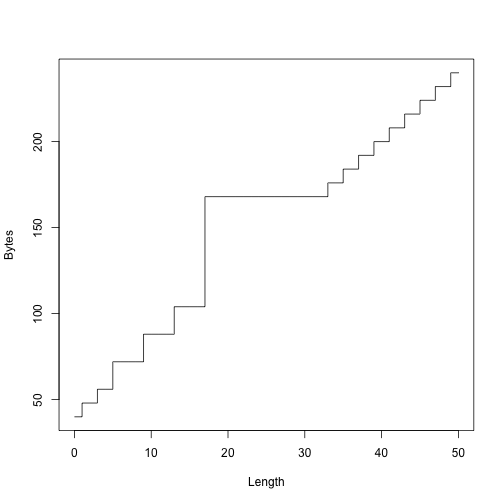
\includegraphics{figures/size-q.pdf}

This isn't just an artefact of integer vectors. Every length 0 vector
occupies 40 bytes of memory:

\begin{Shaded}
\begin{Highlighting}[]
\KeywordTok{object_size}\NormalTok{(}\KeywordTok{numeric}\NormalTok{())}
\CommentTok{#> 40 B}
\KeywordTok{object_size}\NormalTok{(}\KeywordTok{logical}\NormalTok{())}
\CommentTok{#> 40 B}
\KeywordTok{object_size}\NormalTok{(}\KeywordTok{raw}\NormalTok{())}
\CommentTok{#> 40 B}
\KeywordTok{object_size}\NormalTok{(}\KeywordTok{list}\NormalTok{())}
\CommentTok{#> 40 B}
\end{Highlighting}
\end{Shaded}

Those 40 bytes are used to store four components possessed by every
object in R:

\begin{itemize}
\item
  Object metadata (4 bytes). These metadata store the base type
  (e.g.~integer) and information used for debugging and memory
  management.
\item
  Two pointers: one to the next object in memory and one to the previous
  object (2 * 8 bytes). This doubly-linked list makes it easy for
  internal R code to loop through every object in memory.
\item
  A pointer to the attributes (8 bytes).
\end{itemize}

All vectors have three additional components: \indexc{SEXP}

\begin{itemize}
\item
  The length of the vector (4 bytes). By using only 4 bytes, you might
  expect that R could only support vectors up to $2 ^ {4 \times 8 - 1}$
  ($2 ^ {31}$, about two billion) elements. But in R 3.0.0 and later,
  you can actually have vectors up to $2 ^ {52}$ elements.
  \href{http://cran.r-project.org/doc/manuals/R-ints.html\#Long-vectors}{Read
  R-internals} to see how support for long vectors was added without
  having to change the size of this field. \index{long vectors}
  \index{atomic vectors!long}
\item
  The ``true'' length of the vector (4 bytes). This is basically never
  used, except when the object is the hash table used for an
  environment. In that case, the true length represents the allocated
  space, and the length represents the space currently used.
\item
  The data (?? bytes). An empty vector has 0 bytes of data, but it's
  obviously very important otherwise! Numeric vectors occupy 8 bytes for
  every element, integer vectors 4, and complex vectors 16.
\end{itemize}

If you're keeping count you'll notice that this only adds up to 36
bytes. The remaining 4 bytes are used for padding so that each component
starts on an 8 byte (= 64-bit) boundary. Most cpu architectures require
pointers to be aligned in this way, and even if they don't require it,
accessing non-aligned pointers tends to be rather slow. (If you're
interested, you can read more about it in
\href{http://www.catb.org/esr/structure-packing/}{C structure packing}.)

This explains the intercept on the graph. But why does the memory size
grow irregularly? To understand why, you need to know a little bit about
how R requests memory from the operating system. Requesting memory (with
\texttt{malloc()}) is a relatively expensive operation. Having to
request memory every time a small vector is created would slow R down
considerably. Instead, R asks for a big block of memory and then manages
that block itself. This block is called the small vector pool and is
used for vectors less than 128 bytes long. For efficiency and
simplicity, it only allocates vectors that are 8, 16, 32, 48, 64, or 128
bytes long. If we adjust our previous plot to remove the 40 bytes of
overhead, we can see that those values correspond to the jumps in memory
use.

\begin{Shaded}
\begin{Highlighting}[]
\KeywordTok{plot}\NormalTok{(}\DecValTok{0}\NormalTok{:}\DecValTok{50}\NormalTok{, sizes -}\StringTok{ }\DecValTok{40}\NormalTok{, }\DataTypeTok{xlab =} \StringTok{"Length"}\NormalTok{, }
  \DataTypeTok{ylab =} \StringTok{"Bytes excluding overhead"}\NormalTok{, }\DataTypeTok{type =} \StringTok{"n"}\NormalTok{)}
\KeywordTok{abline}\NormalTok{(}\DataTypeTok{h =} \DecValTok{0}\NormalTok{, }\DataTypeTok{col =} \StringTok{"grey80"}\NormalTok{)}
\KeywordTok{abline}\NormalTok{(}\DataTypeTok{h =} \KeywordTok{c}\NormalTok{(}\DecValTok{8}\NormalTok{, }\DecValTok{16}\NormalTok{, }\DecValTok{32}\NormalTok{, }\DecValTok{48}\NormalTok{, }\DecValTok{64}\NormalTok{, }\DecValTok{128}\NormalTok{), }\DataTypeTok{col =} \StringTok{"grey80"}\NormalTok{)}
\KeywordTok{abline}\NormalTok{(}\DataTypeTok{a =} \DecValTok{0}\NormalTok{, }\DataTypeTok{b =} \DecValTok{4}\NormalTok{, }\DataTypeTok{col =} \StringTok{"grey90"}\NormalTok{, }\DataTypeTok{lwd =} \DecValTok{4}\NormalTok{)}
\KeywordTok{lines}\NormalTok{(sizes -}\StringTok{ }\DecValTok{40}\NormalTok{, }\DataTypeTok{type =} \StringTok{"s"}\NormalTok{)}
\end{Highlighting}
\end{Shaded}

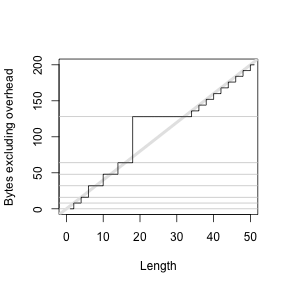
\includegraphics{figures/size-a.pdf}

Beyond 128 bytes, it no longer makes sense for R to manage vectors.
After all, allocating big chunks of memory is something that operating
systems are very good at. Beyond 128 bytes, R will ask for memory in
multiples of 8 bytes. This ensures good alignment.

A subtlety of the size of an object is that components can be shared
across multiple objects. For example, look at the following code:

\begin{Shaded}
\begin{Highlighting}[]
\NormalTok{x <-}\StringTok{ }\DecValTok{1}\NormalTok{:}\FloatTok{1e6}
\KeywordTok{object_size}\NormalTok{(x)}
\CommentTok{#> 4 MB}

\NormalTok{y <-}\StringTok{ }\KeywordTok{list}\NormalTok{(x, x, x)}
\KeywordTok{object_size}\NormalTok{(y)}
\CommentTok{#> 4 MB}
\end{Highlighting}
\end{Shaded}

\texttt{y} isn't three times as big as \texttt{x} because R is smart
enough to not copy \texttt{x} three times; instead it just points to the
existing \texttt{x}.

It's misleading to look at the sizes of \texttt{x} and \texttt{y}
individually. If you want to know how much space they take up together,
you have to supply them to the same \texttt{object\_size()} call:

\begin{Shaded}
\begin{Highlighting}[]
\KeywordTok{object_size}\NormalTok{(x, y)}
\CommentTok{#> 4 MB}
\end{Highlighting}
\end{Shaded}

In this case, \texttt{x} and \texttt{y} together take up the same amount
of space as \texttt{y} alone. This is not always the case. If there are
no shared components, as in the following example, then you can add up
the sizes of individual components to find out the total size:

\begin{Shaded}
\begin{Highlighting}[]
\NormalTok{x1 <-}\StringTok{ }\DecValTok{1}\NormalTok{:}\FloatTok{1e6}
\NormalTok{y1 <-}\StringTok{ }\KeywordTok{list}\NormalTok{(}\DecValTok{1}\NormalTok{:}\FloatTok{1e6}\NormalTok{, }\DecValTok{1}\NormalTok{:}\FloatTok{1e6}\NormalTok{, }\DecValTok{1}\NormalTok{:}\FloatTok{1e6}\NormalTok{)}

\KeywordTok{object_size}\NormalTok{(x1)}
\CommentTok{#> 4 MB}
\KeywordTok{object_size}\NormalTok{(y1)}
\CommentTok{#> 12 MB}
\KeywordTok{object_size}\NormalTok{(x1, y1)}
\CommentTok{#> 16 MB}
\KeywordTok{object_size}\NormalTok{(x1) +}\StringTok{ }\KeywordTok{object_size}\NormalTok{(y1) ==}\StringTok{ }\KeywordTok{object_size}\NormalTok{(x1, y1)}
\CommentTok{#> [1] TRUE}
\end{Highlighting}
\end{Shaded}

The same issue also comes up with strings, because R has a global string
pool. This means that each unique string is only stored in one place,
and therefore character vectors take up less memory than you might
expect: \index{string pool}

\begin{Shaded}
\begin{Highlighting}[]
\KeywordTok{object_size}\NormalTok{(}\StringTok{"banana"}\NormalTok{)}
\CommentTok{#> 96 B}
\KeywordTok{object_size}\NormalTok{(}\KeywordTok{rep}\NormalTok{(}\StringTok{"banana"}\NormalTok{, }\DecValTok{10}\NormalTok{))}
\CommentTok{#> 216 B}
\end{Highlighting}
\end{Shaded}

\subsection{Exercises}

\begin{enumerate}
\def\labelenumi{\arabic{enumi}.}
\item
  Repeat the analysis above for numeric, logical, and complex vectors.
\item
  If a data frame has one million rows, and three variables (two
  numeric, and one integer), how much space will it take up? Work out it
  out from theory, then verify your work by creating a data frame and
  measuring its size.
\item
  Compare the sizes of the elements in the following two lists. Each
  contains basically the same data, but one contains vectors of small
  strings while the other contains a single long string.

\begin{Shaded}
\begin{Highlighting}[]
\NormalTok{vec <-}\StringTok{ }\KeywordTok{lapply}\NormalTok{(}\DecValTok{0}\NormalTok{:}\DecValTok{50}\NormalTok{, function(i) }\KeywordTok{c}\NormalTok{(}\StringTok{"ba"}\NormalTok{, }\KeywordTok{rep}\NormalTok{(}\StringTok{"na"}\NormalTok{, i)))}
\NormalTok{str <-}\StringTok{ }\KeywordTok{lapply}\NormalTok{(vec, paste0, }\DataTypeTok{collapse =} \StringTok{""}\NormalTok{)}
\end{Highlighting}
\end{Shaded}
\item
  Which takes up more memory: a factor (\texttt{x}) or the equivalent
  character vector (\texttt{as.character(x)})? Why?
\item
  Explain the difference in size between \texttt{1:5} and
  \texttt{list(1:5)}.
\end{enumerate}

\hyperdef{}{gc}{\section{Memory usage and garbage collection}\label{gc}}

While \texttt{object\_size()} tells you the size of a single object,
\texttt{pryr::mem\_used()} tells you the total size of all objects in
memory: \indexc{mem\_used()}

\begin{Shaded}
\begin{Highlighting}[]
\KeywordTok{library}\NormalTok{(pryr)}
\KeywordTok{mem_used}\NormalTok{()}
\CommentTok{#> 45.4 MB}
\end{Highlighting}
\end{Shaded}

This number won't agree with the amount of memory reported by your
operating system for a number of reasons:

\begin{enumerate}
\def\labelenumi{\arabic{enumi}.}
\item
  It only includes objects created by R, not the R interpreter itself.
\item
  Both R and the operating system are lazy: they won't reclaim memory
  until it's actually needed. R might be holding on to memory because
  the OS hasn't yet asked for it back.
\item
  R counts the memory occupied by objects but there may be gaps due to
  deleted objects. This problem is known as memory fragmentation.
\end{enumerate}

\texttt{mem\_change()} builds on top of \texttt{mem\_used()} to tell you
how memory changes during code execution. Positive numbers represent an
increase in the memory used by R, and negative numbers represent a
decrease. \indexc{mem\_change()}

\begin{Shaded}
\begin{Highlighting}[]
\CommentTok{# Need about 4 mb to store 1 million integers}
\KeywordTok{mem_change}\NormalTok{(x <-}\StringTok{ }\DecValTok{1}\NormalTok{:}\FloatTok{1e6}\NormalTok{)}
\CommentTok{#> 4.01 MB}
\CommentTok{# We get that memory back when we delete it}
\KeywordTok{mem_change}\NormalTok{(}\KeywordTok{rm}\NormalTok{(x))}
\CommentTok{#> -4 MB}
\end{Highlighting}
\end{Shaded}

Even operations that don't do anything use up a little memory. This is
because R is tracking the history of everything you do. You can ignore
anything on the order of around 2 kB.

\begin{Shaded}
\begin{Highlighting}[]
\KeywordTok{mem_change}\NormalTok{(}\OtherTok{NULL}\NormalTok{)}
\CommentTok{#> 1.47 kB}
\KeywordTok{mem_change}\NormalTok{(}\OtherTok{NULL}\NormalTok{)}
\CommentTok{#> 1.47 kB}
\end{Highlighting}
\end{Shaded}

In some languages, you have to explicitly delete unused objects for
their memory to be returned. R uses an alternative approach: garbage
collection (or GC for short). GC automatically releases memory when an
object is no longer used. It does this by tracking how many names point
to each object, and when there are no names pointing to an object, it
deletes that object. \index{garbage collection}

\begin{Shaded}
\begin{Highlighting}[]
\CommentTok{# Create a big object}
\KeywordTok{mem_change}\NormalTok{(x <-}\StringTok{ }\DecValTok{1}\NormalTok{:}\FloatTok{1e6}\NormalTok{)}
\CommentTok{#> 4 MB}
\CommentTok{# Also point to 1:1e6 from y}
\KeywordTok{mem_change}\NormalTok{(y <-}\StringTok{ }\NormalTok{x)}
\CommentTok{#> -4 MB}
\CommentTok{# Remove x, no memory freed because y is still pointing to it}
\KeywordTok{mem_change}\NormalTok{(}\KeywordTok{rm}\NormalTok{(x))}
\CommentTok{#> 1.42 kB}
\CommentTok{# Now nothing points to it and the memory can be freed}
\KeywordTok{mem_change}\NormalTok{(}\KeywordTok{rm}\NormalTok{(y))}
\CommentTok{#> -4 MB}
\end{Highlighting}
\end{Shaded}

Despite what you might have read elsewhere, there's never any need to
call \texttt{gc()} yourself. R will automatically run garbage collection
whenever it needs more space; if you want to see when that is, call
\texttt{gcinfo(TRUE)}. The only reason you \emph{might} want to call
\texttt{gc()} is to ask R to return memory to the operating system.
However, even that might not have any effect: older versions of Windows
had no way for a program to return memory to the OS. \indexc{gc()}

GC takes care of releasing objects that are no longer used. However, you
do need to be aware of possible memory leaks. A memory leak occurs when
you keep pointing to an object without realising it. In R, the two main
causes of memory leaks are formulas and closures because they both
capture the enclosing environment. The following code illustrates the
problem. In \texttt{f1()}, \texttt{1:1e6} is only referenced inside the
function, so when the function completes the memory is returned and the
net change is 0. The net memory change will be 0. \texttt{f2()} and
\texttt{f3()} both return objects that capture environments, so that
\texttt{x} is not freed when the function completes.
\index{memory!leaks}

\begin{Shaded}
\begin{Highlighting}[]
\NormalTok{f1 <-}\StringTok{ }\NormalTok{function() \{}
  \NormalTok{x <-}\StringTok{ }\DecValTok{1}\NormalTok{:}\FloatTok{1e6}
  \DecValTok{10}
\NormalTok{\}}
\KeywordTok{mem_change}\NormalTok{(x <-}\StringTok{ }\KeywordTok{f1}\NormalTok{())}
\CommentTok{#> 1.38 kB}
\KeywordTok{object_size}\NormalTok{(x)}
\CommentTok{#> 48 B}

\NormalTok{f2 <-}\StringTok{ }\NormalTok{function() \{}
  \NormalTok{x <-}\StringTok{ }\DecValTok{1}\NormalTok{:}\FloatTok{1e6}
  \NormalTok{a ~}\StringTok{ }\NormalTok{b}
\NormalTok{\}}
\KeywordTok{mem_change}\NormalTok{(y <-}\StringTok{ }\KeywordTok{f2}\NormalTok{())}
\CommentTok{#> 4 MB}
\KeywordTok{object_size}\NormalTok{(y)}
\CommentTok{#> 4 MB}

\NormalTok{f3 <-}\StringTok{ }\NormalTok{function() \{}
  \NormalTok{x <-}\StringTok{ }\DecValTok{1}\NormalTok{:}\FloatTok{1e6}
  \NormalTok{function() }\DecValTok{10}
\NormalTok{\}}
\KeywordTok{mem_change}\NormalTok{(z <-}\StringTok{ }\KeywordTok{f3}\NormalTok{())}
\CommentTok{#> 4 MB}
\KeywordTok{object_size}\NormalTok{(z)}
\CommentTok{#> 4.01 MB}
\end{Highlighting}
\end{Shaded}

\hyperdef{}{memory-profiling}{\section{Memory profiling with
lineprof}\label{memory-profiling}}

\texttt{mem\_change()} captures the net change in memory when running a
block of code. Sometimes, however, we may want to measure incremental
change. One way to do this is to use memory profiling to capture usage
every few milliseconds. This functionality is provided by
\texttt{utils::Rprof()} but it doesn't provide a very useful display of
the results. Instead we'll use the
\href{https://github.com/hadley/lineprof}{lineprof} package. It is
powered by \texttt{Rprof()}, but displays the results in a more
informative manner. \index{memory!profiling}

To demonstrate \texttt{lineprof}, we're going to explore a bare-bones
implementation of \texttt{read.delim()} with only three arguments:
\indexc{read\_delim()}

\begin{Shaded}
\begin{Highlighting}[]
\NormalTok{read_delim <-}\StringTok{ }\NormalTok{function(file, }\DataTypeTok{header =} \OtherTok{TRUE}\NormalTok{, }\DataTypeTok{sep =} \StringTok{","}\NormalTok{) \{}
  \CommentTok{# Determine number of fields by reading first line}
  \NormalTok{first <-}\StringTok{ }\KeywordTok{scan}\NormalTok{(file, }\DataTypeTok{what =} \KeywordTok{character}\NormalTok{(}\DecValTok{1}\NormalTok{), }\DataTypeTok{nlines =} \DecValTok{1}\NormalTok{,}
    \DataTypeTok{sep =} \NormalTok{sep, }\DataTypeTok{quiet =} \OtherTok{TRUE}\NormalTok{)}
  \NormalTok{p <-}\StringTok{ }\KeywordTok{length}\NormalTok{(first)}

  \CommentTok{# Load all fields as character vectors}
  \NormalTok{all <-}\StringTok{ }\KeywordTok{scan}\NormalTok{(file, }\DataTypeTok{what =} \KeywordTok{as.list}\NormalTok{(}\KeywordTok{rep}\NormalTok{(}\StringTok{"character"}\NormalTok{, p)),}
    \DataTypeTok{sep =} \NormalTok{sep, }\DataTypeTok{skip =} \NormalTok{if (header) }\DecValTok{1} \NormalTok{else }\DecValTok{0}\NormalTok{, }\DataTypeTok{quiet =} \OtherTok{TRUE}\NormalTok{)}

  \CommentTok{# Convert from strings to appropriate types (never to factors)}
  \NormalTok{all[] <-}\StringTok{ }\KeywordTok{lapply}\NormalTok{(all, type.convert, }\DataTypeTok{as.is =} \OtherTok{TRUE}\NormalTok{)}

  \CommentTok{# Set column names}
  \NormalTok{if (header) \{}
    \KeywordTok{names}\NormalTok{(all) <-}\StringTok{ }\NormalTok{first}
  \NormalTok{\} else \{}
    \KeywordTok{names}\NormalTok{(all) <-}\StringTok{ }\KeywordTok{paste0}\NormalTok{(}\StringTok{"V"}\NormalTok{, }\KeywordTok{seq_along}\NormalTok{(all))}
  \NormalTok{\}}

  \CommentTok{# Convert list into data frame}
  \KeywordTok{as.data.frame}\NormalTok{(all)}
\NormalTok{\}}
\end{Highlighting}
\end{Shaded}

We'll also create a sample csv file:

\begin{Shaded}
\begin{Highlighting}[]
\KeywordTok{library}\NormalTok{(ggplot2)}
\KeywordTok{write.csv}\NormalTok{(diamonds, }\StringTok{"diamonds.csv"}\NormalTok{, }\DataTypeTok{row.names =} \OtherTok{FALSE}\NormalTok{)}
\end{Highlighting}
\end{Shaded}

Using lineprof is straightforward. \texttt{source()} the code, apply
\texttt{lineprof()} to an expression, then use \texttt{shine()} to view
the results. Note that you \emph{must} use \texttt{source()} to load the
code. This is because lineprof uses srcrefs to match up the code and run
times. The needed srcrefs are only created when you load code from disk.

\begin{Shaded}
\begin{Highlighting}[]
\KeywordTok{library}\NormalTok{(lineprof)}

\KeywordTok{source}\NormalTok{(}\StringTok{"code/read-delim.R"}\NormalTok{)}
\NormalTok{prof <-}\StringTok{ }\KeywordTok{lineprof}\NormalTok{(}\KeywordTok{read_delim}\NormalTok{(}\StringTok{"diamonds.csv"}\NormalTok{))}
\KeywordTok{shine}\NormalTok{(prof)}
\end{Highlighting}
\end{Shaded}

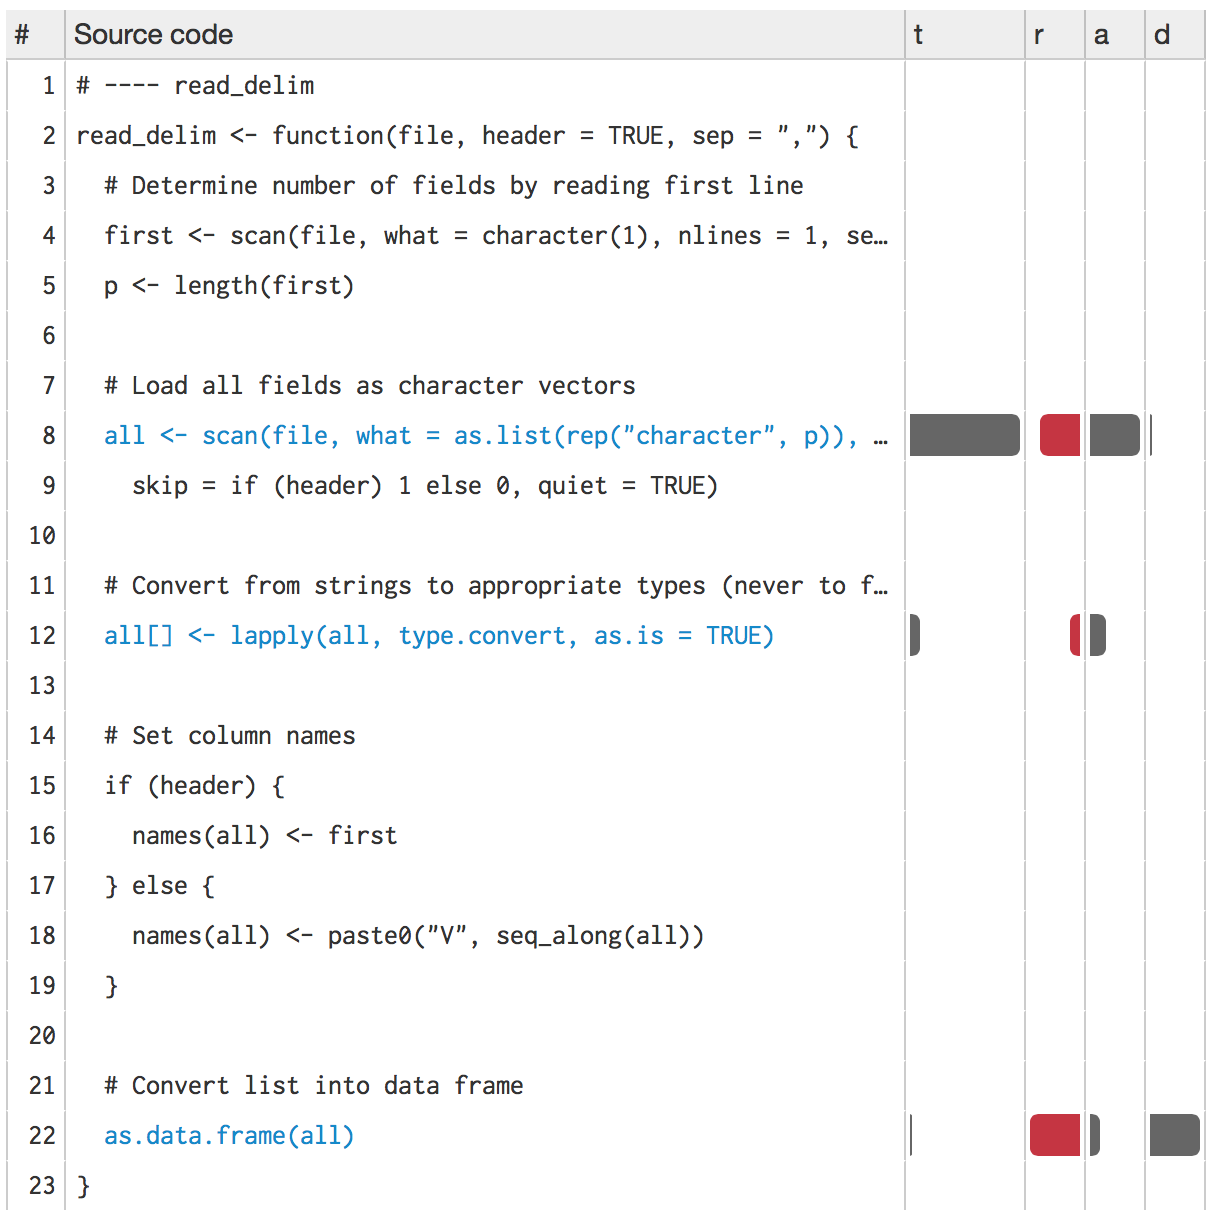
\includegraphics[width=4.35in]{screenshots/memory-lineprof.png}

\texttt{shine()} will also open a new web page (or if you're using
RStudio, a new pane) that shows your source code annotated with
information about memory usage. \texttt{shine()} starts a shiny app
which will ``block'' your R session. To exit, press escape or ctrl +
break.

Next to the source code, four columns provide details about the
performance of the code:

\begin{itemize}
\item
  \texttt{t}, the time (in seconds) spent on that line of code
  (explained in \hyperref[measure-perf]{measuring performance}).
\item
  \texttt{a}, the memory (in megabytes) allocated by that line of code.
\item
  \texttt{r}, the memory (in megabytes) released by that line of code.
  While memory allocation is deterministic, memory release is
  stochastic: it depends on when the GC was run. This means that memory
  release only tells you that the memory released was no longer needed
  before this line.
\item
  \texttt{d}, the number of vector duplications that occurred. A vector
  duplication occurs when R copies a vector as a result of its copy on
  modify semantics.
\end{itemize}

You can hover over any of the bars to get the exact numbers. In this
example, looking at the allocations tells us most of the story:

\begin{itemize}
\item
  \texttt{scan()} allocates about 2.5 MB of memory, which is very close
  to the 2.8 MB of space that the file occupies on disk. You wouldn't
  expect the two numbers to be identical because R doesn't need to store
  the commas and because the global string pool will save some memory.
\item
  Converting the columns allocates another 0.6 MB of memory. You'd also
  expect this step to free some memory because we've converted string
  columns into integer and numeric columns (which occupy less space),
  but we can't see those releases because GC hasn't been triggered yet.
\item
  Finally, calling \texttt{as.data.frame()} on a list allocates about
  1.6 megabytes of memory and performs over 600 duplications. This is
  because \texttt{as.data.frame()} isn't terribly efficient and ends up
  copying the input multiple times. We'll discuss duplication more in
  the next section.
\end{itemize}

There are two downsides to profiling:

\begin{enumerate}
\def\labelenumi{\arabic{enumi}.}
\item
  \texttt{read\_delim()} only takes around half a second, but profiling
  can, at best, capture memory usage every 1 ms. This means we'll only
  get about 500 samples.
\item
  Since GC is lazy, we can never tell exactly when memory is no longer
  needed.
\end{enumerate}

You can work around both problems by using \texttt{torture = TRUE},
which forces R to run GC after every allocation (see
\texttt{gctorture()} for more details). This helps with both problems
because memory is freed as soon as possible, and R runs 10--100x slower.
This effectively makes the resolution of the timer greater, so that you
can see smaller allocations and exactly when memory is no longer needed.

\subsection{Exercises}

\begin{enumerate}
\def\labelenumi{\arabic{enumi}.}
\item
  When the input is a list, we can make a more efficient
  \texttt{as.data.frame()} by using special knowledge. A data frame is a
  list with class \texttt{data.frame} and \texttt{row.names} attribute.
  \texttt{row.names} is either a character vector or vector of
  sequential integers, stored in a special format created by
  \texttt{.set\_row\_names()}. This leads to an alternative
  \texttt{as.data.frame()}:

\begin{Shaded}
\begin{Highlighting}[]
\NormalTok{to_df <-}\StringTok{ }\NormalTok{function(x) \{}
  \KeywordTok{class}\NormalTok{(x) <-}\StringTok{ "data.frame"}
  \KeywordTok{attr}\NormalTok{(x, }\StringTok{"row.names"}\NormalTok{) <-}\StringTok{ }\KeywordTok{.set_row_names}\NormalTok{(}\KeywordTok{length}\NormalTok{(x[[}\DecValTok{1}\NormalTok{]]))}
  \NormalTok{x}
\NormalTok{\}}
\end{Highlighting}
\end{Shaded}

  What impact does this function have on \texttt{read\_delim()}? What
  are the downsides of this function?
\item
  Line profile the following function with \texttt{torture = TRUE}. What
  is surprising? Read the source code of \texttt{rm()} to figure out
  what's going on.

\begin{Shaded}
\begin{Highlighting}[]
\NormalTok{f <-}\StringTok{ }\NormalTok{function(}\DataTypeTok{n =} \FloatTok{1e5}\NormalTok{) \{}
  \NormalTok{x <-}\StringTok{ }\KeywordTok{rep}\NormalTok{(}\DecValTok{1}\NormalTok{, n)}
  \KeywordTok{rm}\NormalTok{(x)}
\NormalTok{\}}
\end{Highlighting}
\end{Shaded}
\end{enumerate}

\hyperdef{}{modification}{\section{Modification in
place}\label{modification}}

What happens to \texttt{x} in the following code?
\index{copy-on-modify!exceptions} \index{avoiding copies}

\begin{Shaded}
\begin{Highlighting}[]
\NormalTok{x <-}\StringTok{ }\DecValTok{1}\NormalTok{:}\DecValTok{10}
\NormalTok{x[}\DecValTok{5}\NormalTok{] <-}\StringTok{ }\DecValTok{10}
\NormalTok{x}
\CommentTok{#>  [1]  1  2  3  4 10  6  7  8  9 10}
\end{Highlighting}
\end{Shaded}

There are two possibilities:

\begin{enumerate}
\def\labelenumi{\arabic{enumi}.}
\item
  R modifies \texttt{x} in place.
\item
  R makes a copy of \texttt{x} to a new location, modifies the copy, and
  then uses the name \texttt{x} to point to the new location.
\end{enumerate}

It turns out that R can do either depending on the circumstances. In the
example above, it will modify in place. But if another variable also
points to \texttt{x}, then R will copy it to a new location. To explore
what's going on in greater detail, we use two tools from the pryr
package. Given the name of a variable, \texttt{address()} will tell us
the variable's location in memory and \texttt{refs()} will tell us how
many names point to that location. \indexc{address()} \indexc{refs()}

\begin{Shaded}
\begin{Highlighting}[]
\KeywordTok{library}\NormalTok{(pryr)}
\NormalTok{x <-}\StringTok{ }\DecValTok{1}\NormalTok{:}\DecValTok{10}
\KeywordTok{c}\NormalTok{(}\KeywordTok{address}\NormalTok{(x), }\KeywordTok{refs}\NormalTok{(x))}
\CommentTok{# [1] "0x103100060" "1"}

\NormalTok{y <-}\StringTok{ }\NormalTok{x}
\KeywordTok{c}\NormalTok{(}\KeywordTok{address}\NormalTok{(y), }\KeywordTok{refs}\NormalTok{(y))}
\CommentTok{# [1] "0x103100060" "2"}
\end{Highlighting}
\end{Shaded}

(Note that if you're using RStudio, \texttt{refs()} will always return
2: the environment browser makes a reference to every object you create
on the command line.)

\texttt{refs()} is only an estimate. It can only distinguish between one
and more than one reference (future versions of R might do better). This
means that \texttt{refs()} returns 2 in both of the following cases:
\index{reference counting}

\begin{Shaded}
\begin{Highlighting}[]
\NormalTok{x <-}\StringTok{ }\DecValTok{1}\NormalTok{:}\DecValTok{5}
\NormalTok{y <-}\StringTok{ }\NormalTok{x}
\KeywordTok{rm}\NormalTok{(y)}
\CommentTok{# Should really be 1, because we've deleted y}
\KeywordTok{refs}\NormalTok{(x)}
\CommentTok{#> [1] 2}

\NormalTok{x <-}\StringTok{ }\DecValTok{1}\NormalTok{:}\DecValTok{5}
\NormalTok{y <-}\StringTok{ }\NormalTok{x}
\NormalTok{z <-}\StringTok{ }\NormalTok{x}
\CommentTok{# Should really be 3}
\KeywordTok{refs}\NormalTok{(x)}
\CommentTok{#> [1] 2}
\end{Highlighting}
\end{Shaded}

When \texttt{refs(x)} is 1, modification will occur in place. When
\texttt{refs(x)} is 2, R will make a copy (this ensures that other
pointers to the object remain unaffected). Note that in the following
example, \texttt{y} keeps pointing to the same location while \texttt{x}
changes.

\begin{Shaded}
\begin{Highlighting}[]
\NormalTok{x <-}\StringTok{ }\DecValTok{1}\NormalTok{:}\DecValTok{10}
\NormalTok{y <-}\StringTok{ }\NormalTok{x}
\KeywordTok{c}\NormalTok{(}\KeywordTok{address}\NormalTok{(x), }\KeywordTok{address}\NormalTok{(y))}
\CommentTok{#> [1] "0x7fa9239c65b0" "0x7fa9239c65b0"}

\NormalTok{x[}\DecValTok{5}\NormalTok{] <-}\StringTok{ }\NormalTok{6L}
\KeywordTok{c}\NormalTok{(}\KeywordTok{address}\NormalTok{(x), }\KeywordTok{address}\NormalTok{(y))}
\CommentTok{#> [1] "0x7fa926be6a08" "0x7fa9239c65b0"}
\end{Highlighting}
\end{Shaded}

Another useful function is \texttt{tracemem()}. It prints a message
every time the traced object is copied: \indexc{tracemem()}

\begin{Shaded}
\begin{Highlighting}[]
\NormalTok{x <-}\StringTok{ }\DecValTok{1}\NormalTok{:}\DecValTok{10}
\CommentTok{# Prints the current memory location of the object}
\KeywordTok{tracemem}\NormalTok{(x)}
\CommentTok{# [1] "<0x7feeaaa1c6b8>"}

\NormalTok{x[}\DecValTok{5}\NormalTok{] <-}\StringTok{ }\NormalTok{6L}

\NormalTok{y <-}\StringTok{ }\NormalTok{x}
\CommentTok{# Prints where it has moved from and to}
\NormalTok{x[}\DecValTok{5}\NormalTok{] <-}\StringTok{ }\NormalTok{6L}
\CommentTok{# tracemem[0x7feeaaa1c6b8 -> 0x7feeaaa1c768]:}
\end{Highlighting}
\end{Shaded}

For interactive use, \texttt{tracemem()} is slightly more useful than
\texttt{refs()}, but because it just prints a message, it's harder to
program with. I don't use it in this book because it interacts poorly
with \href{http://yihui.name/knitr/}{knitr}, the tool I use to
interleave text and code.

Non-primitive functions that touch the object always increment the ref
count. Primitive functions usually don't. (The reasons are a little
complicated, but see the R-devel thread
\href{http://r.789695.n4.nabble.com/Confused-about-NAMED-td4103326.html}{confused
about NAMED}.) \index{primitive functions}

\begin{Shaded}
\begin{Highlighting}[]
\CommentTok{# Touching the object forces an increment}
\NormalTok{f <-}\StringTok{ }\NormalTok{function(x) x}
\NormalTok{\{x <-}\StringTok{ }\DecValTok{1}\NormalTok{:}\DecValTok{10}\NormalTok{; }\KeywordTok{f}\NormalTok{(x); }\KeywordTok{refs}\NormalTok{(x)\}}
\CommentTok{#> [1] 2}

\CommentTok{# Sum is primitive, so no increment}
\NormalTok{\{x <-}\StringTok{ }\DecValTok{1}\NormalTok{:}\DecValTok{10}\NormalTok{; }\KeywordTok{sum}\NormalTok{(x); }\KeywordTok{refs}\NormalTok{(x)\}}
\CommentTok{#> [1] 1}

\CommentTok{# f() and g() never evaluate x, so refs don't increment}
\NormalTok{f <-}\StringTok{ }\NormalTok{function(x) }\DecValTok{10}
\NormalTok{g <-}\StringTok{ }\NormalTok{function(x) }\KeywordTok{substitute}\NormalTok{(x)}

\NormalTok{\{x <-}\StringTok{ }\DecValTok{1}\NormalTok{:}\DecValTok{10}\NormalTok{; }\KeywordTok{f}\NormalTok{(x); }\KeywordTok{refs}\NormalTok{(x)\}}
\CommentTok{#> [1] 1}
\NormalTok{\{x <-}\StringTok{ }\DecValTok{1}\NormalTok{:}\DecValTok{10}\NormalTok{; }\KeywordTok{g}\NormalTok{(x); }\KeywordTok{refs}\NormalTok{(x)\}}
\CommentTok{#> [1] 1}
\end{Highlighting}
\end{Shaded}

Generally, provided that the object is not referred to elsewhere, any
primitive replacement function will modify in place. This includes
\texttt{{[}{[}\textless{}-}, \texttt{{[}\textless{}-},
\texttt{@\textless{}-}, \texttt{\$\textless{}-},
\texttt{attr\textless{}-}, \texttt{attributes\textless{}-},
\texttt{class\textless{}-}, \texttt{dim\textless{}-},
\texttt{dimnames\textless{}-}, \texttt{names\textless{}-}, and
\texttt{levels\textless{}-}. To be precise, all non-primitive functions
increment refs, but a primitive function may be written in such a way
that it doesn't. The rules are sufficiently complicated that there's
little point in trying to memorise them. Instead, you should approach
the problem practically by using \texttt{refs()} and \texttt{address()}
to figure out when objects are being copied.
\index{subsetting|subassignment}

While determining that copies are being made is not hard, preventing
such behaviour is. If you find yourself resorting to exotic tricks to
avoid copies, it may be time to rewrite your function in C++, as
described in \hyperref[rcpp]{Rcpp}.

\subsection{Loops}

For loops in R have a reputation for being slow. Often that slowness is
because you're modifying a copy instead of modifying in place. Consider
the following code. It subtracts the median from each column of a large
data frame: \index{loops!avoiding copies}

\begin{Shaded}
\begin{Highlighting}[]
\NormalTok{x <-}\StringTok{ }\KeywordTok{data.frame}\NormalTok{(}\KeywordTok{matrix}\NormalTok{(}\KeywordTok{runif}\NormalTok{(}\DecValTok{100} \NormalTok{*}\StringTok{ }\FloatTok{1e4}\NormalTok{), }\DataTypeTok{ncol =} \DecValTok{100}\NormalTok{))}
\NormalTok{medians <-}\StringTok{ }\KeywordTok{vapply}\NormalTok{(x, median, }\KeywordTok{numeric}\NormalTok{(}\DecValTok{1}\NormalTok{))}

\NormalTok{for(i in }\KeywordTok{seq_along}\NormalTok{(medians)) \{}
  \NormalTok{x[, i] <-}\StringTok{ }\NormalTok{x[, i] -}\StringTok{ }\NormalTok{medians[i]}
\NormalTok{\}}
\end{Highlighting}
\end{Shaded}

You may be surprised to realise that every iteration of the loop copies
the data frame. We can see that more clearly by using \texttt{address()}
and \texttt{refs()} for a small sample of the loop:

\begin{Shaded}
\begin{Highlighting}[]
\NormalTok{for(i in }\DecValTok{1}\NormalTok{:}\DecValTok{5}\NormalTok{) \{}
  \NormalTok{x[, i] <-}\StringTok{ }\NormalTok{x[, i] -}\StringTok{ }\NormalTok{medians[i]}
  \KeywordTok{print}\NormalTok{(}\KeywordTok{c}\NormalTok{(}\KeywordTok{address}\NormalTok{(x), }\KeywordTok{refs}\NormalTok{(x)))}
\NormalTok{\}}
\CommentTok{#> [1] "0x7fa92502c3e0" "2"             }
\CommentTok{#> [1] "0x7fa92502cdd0" "2"             }
\CommentTok{#> [1] "0x7fa92502d7c0" "2"             }
\CommentTok{#> [1] "0x7fa92502e1b0" "2"             }
\CommentTok{#> [1] "0x7fa92500bfe0" "2"}
\end{Highlighting}
\end{Shaded}

For each iteration, \texttt{x} is moved to a new location so
\texttt{refs(x)} is always 2. This occurs because
\texttt{{[}\textless{}-.data.frame} is not a primitive function, so it
always increments the refs. We can make the function substantially more
efficient by using a list instead of a data frame. Modifying a list uses
primitive functions, so the refs are not incremented and all
modifications occur in place:

\begin{Shaded}
\begin{Highlighting}[]
\NormalTok{y <-}\StringTok{ }\KeywordTok{as.list}\NormalTok{(x)}

\NormalTok{for(i in }\DecValTok{1}\NormalTok{:}\DecValTok{5}\NormalTok{) \{}
  \NormalTok{y[[i]] <-}\StringTok{ }\NormalTok{y[[i]] -}\StringTok{ }\NormalTok{medians[i]}
  \KeywordTok{print}\NormalTok{(}\KeywordTok{c}\NormalTok{(}\KeywordTok{address}\NormalTok{(y), }\KeywordTok{refs}\NormalTok{(y)))}
\NormalTok{\}}
\CommentTok{#> [1] "0x7fa9250238d0" "2"             }
\CommentTok{#> [1] "0x7fa925016850" "2"             }
\CommentTok{#> [1] "0x7fa9250027e0" "2"             }
\CommentTok{#> [1] "0x7fa92501fd60" "2"             }
\CommentTok{#> [1] "0x7fa925006be0" "2"}
\end{Highlighting}
\end{Shaded}

This behaviour was substantially more problematic prior to R 3.1.0,
because every copy of the data frame was a deep copy. This made the
motivating example take around 5 s, compared to 0.01 s today.

\subsection{Exercises}

\begin{enumerate}
\def\labelenumi{\arabic{enumi}.}
\item
  The code below makes one duplication. Where does it occur and why?
  (Hint: look at \texttt{refs(y)}.)

\begin{Shaded}
\begin{Highlighting}[]
\NormalTok{y <-}\StringTok{ }\KeywordTok{as.list}\NormalTok{(x)}
\NormalTok{for(i in }\KeywordTok{seq_along}\NormalTok{(medians)) \{}
  \NormalTok{y[[i]] <-}\StringTok{ }\NormalTok{y[[i]] -}\StringTok{ }\NormalTok{medians[i]}
\NormalTok{\}}
\end{Highlighting}
\end{Shaded}
\item
  The implementation of \texttt{as.data.frame()} in the previous section
  has one big downside. What is it and how could you avoid it?
\end{enumerate}

\chapter{High performance functions with Rcpp}\label{rcpp}

Sometimes R code just isn't fast enough. You've used profiling to figure
out where your bottlenecks are, and you've done everything you can in R,
but your code still isn't fast enough. In this chapter you'll learn how
to improve performance by rewriting key functions in C++. This magic
comes by way of the \href{http://www.rcpp.org/}{Rcpp} package, a
fantastic tool written by Dirk Eddelbuettel and Romain Francois (with
key contributions by Doug Bates, John Chambers, and JJ Allaire). Rcpp
makes it very simple to connect C++ to R. While it is \emph{possible} to
write C or Fortran code for use in R, it will be painful by comparison.
Rcpp provides a clean, approachable API that lets you write
high-performance code, insulated from R's arcane C API. \index{Rcpp}
\index{C++}

Typical bottlenecks that C++ can address include:

\begin{itemize}
\item
  Loops that can't be easily vectorised because subsequent iterations
  depend on previous ones.
\item
  Recursive functions, or problems which involve calling functions
  millions of times. The overhead of calling a function in C++ is much
  lower than that in R.
\item
  Problems that require advanced data structures and algorithms that R
  doesn't provide. Through the standard template library (STL), C++ has
  efficient implementations of many important data structures, from
  ordered maps to double-ended queues.
\end{itemize}

The aim of this chapter is to discuss only those aspects of C++ and Rcpp
that are absolutely necessary to help you eliminate bottlenecks in your
code. We won't spend much time on advanced features like object oriented
programming or templates because the focus is on writing small,
self-contained functions, not big programs. A working knowledge of C++
is helpful, but not essential. Many good tutorials and references are
freely available, including \url{http://www.learncpp.com/} and
\url{http://www.cplusplus.com/}. For more advanced topics, the
\emph{Effective C++} series by Scott Meyers is popular choice. You may
also enjoy Dirk Eddelbuettel's
\href{http://www.springer.com/statistics/computational+statistics/book/978-1-4614-6867-7}{\emph{Seamless
R and C++ integration with Rcpp}}, which goes into much greater detail
into all aspects of Rcpp.

\paragraph{Outline}

\begin{itemize}
\item
  \hyperref[rcpp-intro]{Getting started with C++} teaches you how to
  write C++ by converting simple R functions to their C++ equivalents.
  You'll learn how C++ differs from R, and what the key scalar, vector,
  and matrix classes are called.
\item
  \hyperref[sourceCpp]{Using sourceCpp} shows you how to use
  \texttt{sourceCpp()} to load a C++ file from disk in the same way you
  use \texttt{source()} to load a file of R code.
\item
  \hyperref[rcpp-classes]{Attributes \& other classes} discusses how to
  modify attributes from Rcpp, and mentions some of the other important
  classes.
\item
  \hyperref[rcpp-na]{Missing values} teaches you how to work with R's
  missing values in C++.
\item
  \hyperref[rcpp-sugar]{Rcpp sugar} discusses Rcpp ``sugar'', which
  allows you to avoid loops in C++ and write code that looks very
  similar to vectorised R code.
\item
  \hyperref[stl]{The STL} shows you how to use some of the most
  important data structures and algorithms from the standard template
  library, or STL, built-in to C++.
\item
  \hyperref[rcpp-case-studies]{Case studies} shows two real case studies
  where Rcpp was used to get considerable performance improvements.
\item
  \hyperref[rcpp-package]{Putting Rcpp in a package} teaches you how to
  add C++ code to a package.
\item
  \hyperref[rcpp-more]{Learning more} concludes the chapter with
  pointers to more resources to help you learn Rcpp and C++.
\end{itemize}

\paragraph{Prerequistes}

All examples in this chapter need version 0.10.1 or above of the
\texttt{Rcpp} package. This version includes \texttt{cppFunction()} and
\texttt{sourceCpp()}, which makes it very easy to connect C++ to R.
Install the latest version of Rcpp from CRAN with
\texttt{install.packages("Rcpp")}.

You'll also need a working C++ compiler. To get it:

\begin{itemize}
\itemsep1pt\parskip0pt\parsep0pt
\item
  On Windows, install
  \href{http://cran.r-project.org/bin/windows/Rtools/}{Rtools}.
\item
  On Mac, install Xcode from the app store.
\item
  On Linux, \texttt{sudo apt-get install r-base-dev} or similar.
\end{itemize}

\hyperdef{}{rcpp-intro}{\section{Getting started with
C++}\label{rcpp-intro}}

\texttt{cppFunction()} allows you to write C++ functions in R:
\indexc{cppFunction()}

\begin{Shaded}
\begin{Highlighting}[]
\KeywordTok{library}\NormalTok{(Rcpp)}
\CommentTok{#> }
\CommentTok{#> Attaching package: 'Rcpp'}
\CommentTok{#> }
\CommentTok{#> The following object is masked from 'package:inline':}
\CommentTok{#> }
\CommentTok{#>     registerPlugin}
\KeywordTok{cppFunction}\NormalTok{(}\StringTok{'int add(int x, int y, int z) \{}
\StringTok{  int sum = x + y + z;}
\StringTok{  return sum;}
\StringTok{\}'}\NormalTok{)}
\CommentTok{# add works like a regular R function}
\NormalTok{add}
\CommentTok{#> function (x, y, z) }
\CommentTok{#> .Primitive(".Call")(<pointer: 0x10fff9e10>, x, y, z)}
\KeywordTok{add}\NormalTok{(}\DecValTok{1}\NormalTok{, }\DecValTok{2}\NormalTok{, }\DecValTok{3}\NormalTok{)}
\CommentTok{#> [1] 6}
\end{Highlighting}
\end{Shaded}

When you run this code, Rcpp will compile the C++ code and construct an
R function that connects to the compiled C++ function. We're going to
use this simple interface to learn how to write C++. C++ is a large
language, and there's no way to cover it all in just one chapter.
Instead, you'll get the basics so that you can start writing useful
functions to address bottlenecks in your R code.

The following sections will teach you the basics by translating simple R
functions to their C++ equivalents. We'll start simple with a function
that has no inputs and a scalar output, and then get progressively more
complicated:

\begin{itemize}
\itemsep1pt\parskip0pt\parsep0pt
\item
  Scalar input and scalar output
\item
  Vector input and scalar output
\item
  Vector input and vector output
\item
  Matrix input and vector output
\end{itemize}

\subsection{No inputs, scalar output}

Let's start with a very simple function. It has no arguments and always
returns the integer 1:

\begin{Shaded}
\begin{Highlighting}[]
\NormalTok{one <-}\StringTok{ }\NormalTok{function() 1L}
\end{Highlighting}
\end{Shaded}

The equivalent C++ function is:

\begin{Shaded}
\begin{Highlighting}[]
\DataTypeTok{int} \NormalTok{one() \{}
  \KeywordTok{return} \DecValTok{1}\NormalTok{;}
\NormalTok{\}}
\end{Highlighting}
\end{Shaded}

We can compile and use this from R with \texttt{cppFunction}

\begin{Shaded}
\begin{Highlighting}[]
\KeywordTok{cppFunction}\NormalTok{(}\StringTok{'int one() \{}
\StringTok{  return 1;}
\StringTok{\}'}\NormalTok{)}
\end{Highlighting}
\end{Shaded}

This small function illustrates a number of important differences
between R and C++:

\begin{itemize}
\item
  The syntax to create a function looks like the syntax to call a
  function; you don't use assignment to create functions as you do in R.
\item
  You must declare the type of output the function returns. This
  function returns an \texttt{int} (a scalar integer). The classes for
  the most common types of R vectors are: \texttt{NumericVector},
  \texttt{IntegerVector}, \texttt{CharacterVector}, and
  \texttt{LogicalVector}.
\item
  Scalars and vectors are different. The scalar equivalents of numeric,
  integer, character, and logical vectors are: \texttt{double},
  \texttt{int}, \texttt{String}, and \texttt{bool}.
\item
  You must use an explicit \texttt{return} statement to return a value
  from a function.
\item
  Every statement is terminated by a \texttt{;}.
\end{itemize}

\subsection{Scalar input, scalar output}

The next example function implements a scalar version of the
\texttt{sign()} function which returns 1 if the input is positive, and
-1 if it's negative:

\begin{Shaded}
\begin{Highlighting}[]
\NormalTok{signR <-}\StringTok{ }\NormalTok{function(x) \{}
  \NormalTok{if (x >}\StringTok{ }\DecValTok{0}\NormalTok{) \{}
    \DecValTok{1}
  \NormalTok{\} else if (x ==}\StringTok{ }\DecValTok{0}\NormalTok{) \{}
    \DecValTok{0}
  \NormalTok{\} else \{}
    \NormalTok{-}\DecValTok{1}
  \NormalTok{\}}
\NormalTok{\}}

\KeywordTok{cppFunction}\NormalTok{(}\StringTok{'int signC(int x) \{}
\StringTok{  if (x > 0) \{}
\StringTok{    return 1;}
\StringTok{  \} else if (x == 0) \{}
\StringTok{    return 0;}
\StringTok{  \} else \{}
\StringTok{    return -1;}
\StringTok{  \}}
\StringTok{\}'}\NormalTok{)}
\end{Highlighting}
\end{Shaded}

In the C++ version:

\begin{itemize}
\item
  We declare the type of each input in the same way we declare the type
  of the output. While this makes the code a little more verbose, it
  also makes it very obvious what type of input the function needs.
\item
  The \texttt{if} syntax is identical --- while there are some big
  differences between R and C++, there are also lots of similarities!
  C++ also has a \texttt{while} statement that works the same way as
  R's. As in R you can use \texttt{break} to exit the loop, but to skip
  one iteration you need to use \texttt{continue} instead of
  \texttt{next}.
\end{itemize}

\subsection{Vector input, scalar output}

One big difference between R and C++ is that the cost of loops is much
lower in C++. For example, we could implement the \texttt{sum} function
in R using a loop. If you've been programming in R a while, you'll
probably have a visceral reaction to this function!

\begin{Shaded}
\begin{Highlighting}[]
\NormalTok{sumR <-}\StringTok{ }\NormalTok{function(x) \{}
  \NormalTok{total <-}\StringTok{ }\DecValTok{0}
  \NormalTok{for (i in }\KeywordTok{seq_along}\NormalTok{(x)) \{}
    \NormalTok{total <-}\StringTok{ }\NormalTok{total +}\StringTok{ }\NormalTok{x[i]}
  \NormalTok{\}}
  \NormalTok{total}
\NormalTok{\}}
\end{Highlighting}
\end{Shaded}

In C++, loops have very little overhead, so it's fine to use them. In
\hyperref[stl]{STL}, you'll see alternatives to \texttt{for} loops that
more clearly express your intent; they're not faster, but they can make
your code easier to understand.

\begin{Shaded}
\begin{Highlighting}[]
\KeywordTok{cppFunction}\NormalTok{(}\StringTok{'double sumC(NumericVector x) \{}
\StringTok{  int n = x.size();}
\StringTok{  double total = 0;}
\StringTok{  for(int i = 0; i < n; ++i) \{}
\StringTok{    total += x[i];}
\StringTok{  \}}
\StringTok{  return total;}
\StringTok{\}'}\NormalTok{)}
\end{Highlighting}
\end{Shaded}

The C++ version is similar, but:

\begin{itemize}
\item
  To find the length of the vector, we use the \texttt{.size()} method,
  which returns an integer. C++ methods are called with \texttt{.}
  (i.e., a full stop).
\item
  The \texttt{for} statement has a different syntax:
  \texttt{for(init; check; increment)}. This loop is initialised by
  creating a new variable called \texttt{i} with value 0. Before each
  iteration we check that \texttt{i \textless{} n}, and terminate the
  loop if it's not. After each iteration, we increment the value of
  \texttt{i} by one, using the special prefix operator \texttt{++} which
  increases the value of \texttt{i} by 1.
\item
  In C++, vector indices start at 0. I'll say this again because it's so
  important: \textbf{IN C++, VECTOR INDICES START AT 0}! This is a very
  common source of bugs when converting R functions to C++.
\item
  Use \texttt{=} for assignment, not \texttt{\textless{}-}.
\item
  C++ provides operators that modify in-place:
  \texttt{total += x{[}i{]}} is equivalent to
  \texttt{total = total + x{[}i{]}}. Similar in-place operators are
  \texttt{-=}, \texttt{*=}, and \texttt{/=}.
\end{itemize}

This is a good example of where C++ is much more efficient than R. As
shown by the following microbenchmark, \texttt{sumC()} is competitive
with the built-in (and highly optimised) \texttt{sum()}, while
\texttt{sumR()} is several orders of magnitude slower.

\begin{Shaded}
\begin{Highlighting}[]
\NormalTok{x <-}\StringTok{ }\KeywordTok{runif}\NormalTok{(}\FloatTok{1e3}\NormalTok{)}
\KeywordTok{microbenchmark}\NormalTok{(}
  \KeywordTok{sum}\NormalTok{(x),}
  \KeywordTok{sumC}\NormalTok{(x),}
  \KeywordTok{sumR}\NormalTok{(x)}
\NormalTok{)}
\CommentTok{#> Unit: microseconds}
\CommentTok{#>     expr    min     lq median     uq      max neval}
\CommentTok{#>   sum(x)   1.07   1.33   1.66   1.95     6.24   100}
\CommentTok{#>  sumC(x)   2.49   2.99   3.54   4.36    21.50   100}
\CommentTok{#>  sumR(x) 333.00 367.00 388.00 428.00 1,390.00   100}
\end{Highlighting}
\end{Shaded}

\subsection{Vector input, vector output}

Next we'll create a function that computes the Euclidean distance
between a value and a vector of values:

\begin{Shaded}
\begin{Highlighting}[]
\NormalTok{pdistR <-}\StringTok{ }\NormalTok{function(x, ys) \{}
  \KeywordTok{sqrt}\NormalTok{((x -}\StringTok{ }\NormalTok{ys) ^}\StringTok{ }\DecValTok{2}\NormalTok{)}
\NormalTok{\}}
\end{Highlighting}
\end{Shaded}

It's not obvious that we want \texttt{x} to be a scalar from the
function definition. We'd need to make that clear in the documentation.
That's not a problem in the C++ version because we have to be explicit
about types:

\begin{Shaded}
\begin{Highlighting}[]
\KeywordTok{cppFunction}\NormalTok{(}\StringTok{'NumericVector pdistC(double x, NumericVector ys) \{}
\StringTok{  int n = ys.size();}
\StringTok{  NumericVector out(n);}

\StringTok{  for(int i = 0; i < n; ++i) \{}
\StringTok{    out[i] = sqrt(pow(ys[i] - x, 2.0));}
\StringTok{  \}}
\StringTok{  return out;}
\StringTok{\}'}\NormalTok{)}
\end{Highlighting}
\end{Shaded}

This function introduces only a few new concepts:

\begin{itemize}
\item
  We create a new numeric vector of length \texttt{n} with a
  constructor: \texttt{NumericVector out(n)}. Another useful way of
  making a vector is to copy an existing one:
  \texttt{NumericVector zs = clone(ys)}.
\item
  C++ uses \texttt{pow()}, not \texttt{\^{}}, for exponentiation.
\end{itemize}

Note that because the R version is fully vectorised, it's already going
to be fast. On my computer, it takes around 8 ms with a 1 million
element \texttt{y} vector. The C++ function is twice as fast,
\textasciitilde{}4 ms, but assuming it took you 10 minutes to write the
C++ function, you'd need to run it \textasciitilde{}150,000 times to
make rewriting worthwhile. The reason why the C++ function is faster is
subtle, and relates to memory management. The R version needs to create
an intermediate vector the same length as y (\texttt{x - ys}), and
allocating memory is an expensive operation. The C++ function avoids
this overhead because it uses an intermediate scalar.

In the sugar section, you'll see how to rewrite this function to take
advantage of Rcpp's vectorised operations so that the C++ code is almost
as concise as R code.

\subsection{Matrix input, vector output}

Each vector type has a matrix equivalent: \texttt{NumericMatrix},
\texttt{IntegerMatrix}, \texttt{CharacterMatrix}, and
\texttt{LogicalMatrix}. Using them is straightforward. For example, we
could create a function that reproduces \texttt{rowSums()}:

\begin{Shaded}
\begin{Highlighting}[]
\KeywordTok{cppFunction}\NormalTok{(}\StringTok{'NumericVector rowSumsC(NumericMatrix x) \{}
\StringTok{  int nrow = x.nrow(), ncol = x.ncol();}
\StringTok{  NumericVector out(nrow);}

\StringTok{  for (int i = 0; i < nrow; i++) \{}
\StringTok{    double total = 0;}
\StringTok{    for (int j = 0; j < ncol; j++) \{}
\StringTok{      total += x(i, j);}
\StringTok{    \}}
\StringTok{    out[i] = total;}
\StringTok{  \}}
\StringTok{  return out;}
\StringTok{\}'}\NormalTok{)}
\KeywordTok{set.seed}\NormalTok{(}\DecValTok{1014}\NormalTok{)}
\NormalTok{x <-}\StringTok{ }\KeywordTok{matrix}\NormalTok{(}\KeywordTok{sample}\NormalTok{(}\DecValTok{100}\NormalTok{), }\DecValTok{10}\NormalTok{)}
\KeywordTok{rowSums}\NormalTok{(x)}
\CommentTok{#>  [1] 458 558 488 458 536 537 488 491 508 528}
\KeywordTok{rowSumsC}\NormalTok{(x)}
\CommentTok{#>  [1] 458 558 488 458 536 537 488 491 508 528}
\end{Highlighting}
\end{Shaded}

The main differences:

\begin{itemize}
\item
  In C++, you subset a matrix with \texttt{()}, not \texttt{{[}{]}}.
\item
  Use \texttt{.nrow()} and \texttt{.ncol()} \emph{methods} to get the
  dimensions of a matrix.
\end{itemize}

\hyperdef{}{sourceCpp}{\subsection{Using sourceCpp}\label{sourceCpp}}

So far, we've used inline C++ with \texttt{cppFunction()}. This makes
presentation simpler, but for real problems, it's usually easier to use
stand-alone C++ files and then source them into R using
\texttt{sourceCpp()}. This lets you take advantage of text editor
support for C++ files (e.g., syntax highlighting) as well as making it
easier to identify the line numbers in compilation errors.
\indexc{sourceCpp()}

Your stand-alone C++ file should have extension \texttt{.cpp}, and needs
to start with:

\begin{Shaded}
\begin{Highlighting}[]
\OtherTok{#include <Rcpp.h>}
\KeywordTok{using} \KeywordTok{namespace} \NormalTok{Rcpp;}
\end{Highlighting}
\end{Shaded}

And for each function that you want available within R, you need to
prefix it with:

\begin{Shaded}
\begin{Highlighting}[]
\CommentTok{// [[Rcpp::export]]}
\end{Highlighting}
\end{Shaded}

Note that the space is mandatory.

If you're familiar with roxygen2, you might wonder how this relates to
\texttt{@export}. \texttt{Rcpp::export} controls whether a function is
exported from C++ to R; \texttt{@export} controls whether a function is
exported from a package and made available to the user.

You can embed R code in special C++ comment blocks. This is really
convenient if you want to run some test code:

\begin{Shaded}
\begin{Highlighting}[]
\CommentTok{/*** R}
\CommentTok{# This is R code}
\CommentTok{*/}
\end{Highlighting}
\end{Shaded}

The R code is run with \texttt{source(echo = TRUE)} so you don't need to
explicitly print output.

To compile the C++ code, use \texttt{sourceCpp("path/to/file.cpp")}.
This will create the matching R functions and add them to your current
session. Note that these functions can not be saved in a \texttt{.Rdata}
file and reloaded in a later session; they must be recreated each time
you restart R. For example, running \texttt{sourceCpp()} on the
following file implements mean in C++ and then compares it to the
built-in \texttt{mean()}:

\begin{Shaded}
\begin{Highlighting}[]
\OtherTok{#include <Rcpp.h>}
\KeywordTok{using} \KeywordTok{namespace} \NormalTok{Rcpp;}

\CommentTok{// [[Rcpp::export]]}
\DataTypeTok{double} \NormalTok{meanC(NumericVector x) \{}
  \DataTypeTok{int} \NormalTok{n = x.size();}
  \DataTypeTok{double} \NormalTok{total = }\DecValTok{0}\NormalTok{;}

  \KeywordTok{for}\NormalTok{(}\DataTypeTok{int} \NormalTok{i = }\DecValTok{0}\NormalTok{; i < n; ++i) \{}
    \NormalTok{total += x[i];}
  \NormalTok{\}}
  \KeywordTok{return} \NormalTok{total / n;}
\NormalTok{\}}

\CommentTok{/*** R}
\CommentTok{library(microbenchmark)}
\CommentTok{x <- runif(1e5)}
\CommentTok{microbenchmark(}
\CommentTok{  mean(x),}
\CommentTok{  meanC(x)}
\CommentTok{)}
\CommentTok{*/}
\end{Highlighting}
\end{Shaded}

NB: if you run this code yourself, you'll notice that \texttt{meanC()}
is much faster than the built-in \texttt{mean()}. This is because it
trades numerical accuracy for speed.

For the remainder of this chapter C++ code will be presented stand-alone
rather than wrapped in a call to \texttt{cppFunction}. If you want to
try compiling and/or modifying the examples you should paste them into a
C++ source file that includes the elements described above.

\subsection{Exercises}

With the basics of C++ in hand, it's now a great time to practice by
reading and writing some simple C++ functions. For each of the following
functions, read the code and figure out what the corresponding base R
function is. You might not understand every part of the code yet, but
you should be able to figure out the basics of what the function does.

\begin{Shaded}
\begin{Highlighting}[]
\DataTypeTok{double} \NormalTok{f1(NumericVector x) \{}
  \DataTypeTok{int} \NormalTok{n = x.size();}
  \DataTypeTok{double} \NormalTok{y = }\DecValTok{0}\NormalTok{;}

  \KeywordTok{for}\NormalTok{(}\DataTypeTok{int} \NormalTok{i = }\DecValTok{0}\NormalTok{; i < n; ++i) \{}
    \NormalTok{y += x[i] / n;}
  \NormalTok{\}}
  \KeywordTok{return} \NormalTok{y;}
\NormalTok{\}}

\NormalTok{NumericVector f2(NumericVector x) \{}
  \DataTypeTok{int} \NormalTok{n = x.size();}
  \NormalTok{NumericVector out(n);}

  \NormalTok{out[}\DecValTok{0}\NormalTok{] = x[}\DecValTok{0}\NormalTok{];}
  \KeywordTok{for}\NormalTok{(}\DataTypeTok{int} \NormalTok{i = }\DecValTok{1}\NormalTok{; i < n; ++i) \{}
    \NormalTok{out[i] = out[i - }\DecValTok{1}\NormalTok{] + x[i];}
  \NormalTok{\}}
  \KeywordTok{return} \NormalTok{out;}
\NormalTok{\}}

\DataTypeTok{bool} \NormalTok{f3(LogicalVector x) \{}
  \DataTypeTok{int} \NormalTok{n = x.size();}

  \KeywordTok{for}\NormalTok{(}\DataTypeTok{int} \NormalTok{i = }\DecValTok{0}\NormalTok{; i < n; ++i) \{}
    \KeywordTok{if} \NormalTok{(x[i]) }\KeywordTok{return} \KeywordTok{true}\NormalTok{;}
  \NormalTok{\}}
  \KeywordTok{return} \KeywordTok{false}\NormalTok{;}
\NormalTok{\}}

\DataTypeTok{int} \NormalTok{f4(Function pred, List x) \{}
  \DataTypeTok{int} \NormalTok{n = x.size();}

  \KeywordTok{for}\NormalTok{(}\DataTypeTok{int} \NormalTok{i = }\DecValTok{0}\NormalTok{; i < n; ++i) \{}
    \NormalTok{LogicalVector res = pred(x[i]);}
    \KeywordTok{if} \NormalTok{(res[}\DecValTok{0}\NormalTok{]) }\KeywordTok{return} \NormalTok{i + }\DecValTok{1}\NormalTok{;}
  \NormalTok{\}}
  \KeywordTok{return} \DecValTok{0}\NormalTok{;}
\NormalTok{\}}

\NormalTok{NumericVector f5(NumericVector x, NumericVector y) \{}
  \DataTypeTok{int} \NormalTok{n = std::max(x.size(), y.size());}
  \NormalTok{NumericVector x1 = rep_len(x, n);}
  \NormalTok{NumericVector y1 = rep_len(y, n);}

  \NormalTok{NumericVector out(n);}

  \KeywordTok{for} \NormalTok{(}\DataTypeTok{int} \NormalTok{i = }\DecValTok{0}\NormalTok{; i < n; ++i) \{}
    \NormalTok{out[i] = std::min(x1[i], y1[i]);}
  \NormalTok{\}}

  \KeywordTok{return} \NormalTok{out;}
\NormalTok{\}}
\end{Highlighting}
\end{Shaded}

To practice your function writing skills, convert the following
functions into C++. For now, assume the inputs have no missing values.

\begin{enumerate}
\def\labelenumi{\arabic{enumi}.}
\item
  \texttt{all()}
\item
  \texttt{cumprod()}, \texttt{cummin()}, \texttt{cummax()}.
\item
  \texttt{diff()}. Start by assuming lag 1, and then generalise for lag
  \texttt{n}.
\item
  \texttt{range}.
\item
  \texttt{var}. Read about the approaches you can take on
  \href{http://en.wikipedia.org/wiki/Algorithms_for_calculating_variance}{wikipedia}.
  Whenever implementing a numerical algorithm, it's always good to check
  what is already known about the problem.
\end{enumerate}

\hyperdef{}{rcpp-classes}{\section{Attributes and other
classes}\label{rcpp-classes}}

You've already seen the basic vector classes (\texttt{IntegerVector},
\texttt{NumericVector}, \texttt{LogicalVector},
\texttt{CharacterVector}) and their scalar (\texttt{int},
\texttt{double}, \texttt{bool}, \texttt{String}) and matrix
(\texttt{IntegerMatrix}, \texttt{NumericMatrix}, \texttt{LogicalMatrix},
\texttt{CharacterMatrix}) equivalents.

All R objects have attributes, which can be queried and modified with
\texttt{.attr()}. Rcpp also provides \texttt{.names()} as an alias for
the name attribute. The following code snippet illustrates these
methods. Note the use of \texttt{::create()}, a \emph{class} method.
This allows you to create an R vector from C++ scalar values:
\index{attributes!in C++ } \index{names!in C++}

\begin{Shaded}
\begin{Highlighting}[]
\OtherTok{#include <Rcpp.h>}
\KeywordTok{using} \KeywordTok{namespace} \NormalTok{Rcpp;}

\CommentTok{// [[Rcpp::export]]}
\NormalTok{NumericVector attribs() \{}
  \NormalTok{NumericVector out = NumericVector::create(}\DecValTok{1}\NormalTok{, }\DecValTok{2}\NormalTok{, }\DecValTok{3}\NormalTok{);}

  \NormalTok{out.names() = CharacterVector::create(}\StringTok{"a"}\NormalTok{, }\StringTok{"b"}\NormalTok{, }\StringTok{"c"}\NormalTok{);}
  \NormalTok{out.attr(}\StringTok{"my-attr"}\NormalTok{) = }\StringTok{"my-value"}\NormalTok{;}
  \NormalTok{out.attr(}\StringTok{"class"}\NormalTok{) = }\StringTok{"my-class"}\NormalTok{;}

  \KeywordTok{return} \NormalTok{out;}
\NormalTok{\}}
\end{Highlighting}
\end{Shaded}

For S4 objects, \texttt{.slot()} plays a similar role to
\texttt{.attr()}.

\subsection{Lists and data frames}

Rcpp also provides classes \texttt{List} and \texttt{DataFrame}, but
they are more useful for output than input. This is because lists and
data frames can contain arbitrary classes but C++ needs to know their
classes in advance. If the list has known structure (e.g., it's an S3
object), you can extract the components and manually convert them to
their C++ equivalents with \texttt{as()}. For example, the object
created by \texttt{lm()}, the function that fits a linear model, is a
list whose components are always of the same type. The following code
illustrates how you might extract the mean percentage error
(\texttt{mpe()}) of a linear model. This isn't a good example of when to
use C++, because it's so easily implemented in R, but it shows how to
work with an important S3 class. Note the use of \texttt{.inherits()}
and the \texttt{stop()} to check that the object really is a linear
model. \index{lists!in C++} \index{data frames!in C++}

\begin{Shaded}
\begin{Highlighting}[]
\OtherTok{#include <Rcpp.h>}
\KeywordTok{using} \KeywordTok{namespace} \NormalTok{Rcpp;}

\CommentTok{// [[Rcpp::export]]}
\DataTypeTok{double} \NormalTok{mpe(List mod) \{}
  \KeywordTok{if} \NormalTok{(!mod.inherits(}\StringTok{"lm"}\NormalTok{)) stop(}\StringTok{"Input must be a linear model"}\NormalTok{);}

  \NormalTok{NumericVector resid = as<NumericVector>(mod[}\StringTok{"residuals"}\NormalTok{]);}
  \NormalTok{NumericVector fitted = as<NumericVector>(mod[}\StringTok{"fitted.values"}\NormalTok{]);}

  \DataTypeTok{int} \NormalTok{n = resid.size();}
  \DataTypeTok{double} \NormalTok{err = }\DecValTok{0}\NormalTok{;}
  \KeywordTok{for}\NormalTok{(}\DataTypeTok{int} \NormalTok{i = }\DecValTok{0}\NormalTok{; i < n; ++i) \{}
    \NormalTok{err += resid[i] / (fitted[i] + resid[i]);}
  \NormalTok{\}}
  \KeywordTok{return} \NormalTok{err / n;}
\NormalTok{\}}
\end{Highlighting}
\end{Shaded}

\begin{Shaded}
\begin{Highlighting}[]
\NormalTok{mod <-}\StringTok{ }\KeywordTok{lm}\NormalTok{(mpg ~}\StringTok{ }\NormalTok{wt, }\DataTypeTok{data =} \NormalTok{mtcars)}
\KeywordTok{mpe}\NormalTok{(mod)}
\CommentTok{#> [1] -0.0154}
\end{Highlighting}
\end{Shaded}

\subsection{Functions}\label{functions-rcpp}

You can put R functions in an object of type \texttt{Function}. This
makes calling an R function from C++ straightforward. We first define
our C++ function: \index{functions!in C++}

\begin{Shaded}
\begin{Highlighting}[]
\OtherTok{#include <Rcpp.h>}
\KeywordTok{using} \KeywordTok{namespace} \NormalTok{Rcpp;}

\CommentTok{// [[Rcpp::export]]}
\NormalTok{RObject callWithOne(Function f) \{}
  \KeywordTok{return} \NormalTok{f(}\DecValTok{1}\NormalTok{);}
\NormalTok{\}}
\end{Highlighting}
\end{Shaded}

Then call it from R:

\begin{Shaded}
\begin{Highlighting}[]
\KeywordTok{callWithOne}\NormalTok{(function(x) x +}\StringTok{ }\DecValTok{1}\NormalTok{)}
\CommentTok{#> [1] 2}
\KeywordTok{callWithOne}\NormalTok{(paste)}
\CommentTok{#> [1] "1"}
\end{Highlighting}
\end{Shaded}

What type of object does an R function return? We don't know, so we use
the catchall type \texttt{RObject}. An alternative is to return a
\texttt{List}. For example, the following code is a basic implementation
of \texttt{lapply} in C++:

\begin{Shaded}
\begin{Highlighting}[]
\OtherTok{#include <Rcpp.h>}
\KeywordTok{using} \KeywordTok{namespace} \NormalTok{Rcpp;}

\CommentTok{// [[Rcpp::export]]}
\NormalTok{List lapply1(List input, Function f) \{}
  \DataTypeTok{int} \NormalTok{n = input.size();}
  \NormalTok{List out(n);}

  \KeywordTok{for}\NormalTok{(}\DataTypeTok{int} \NormalTok{i = }\DecValTok{0}\NormalTok{; i < n; i++) \{}
    \NormalTok{out[i] = f(input[i]);}
  \NormalTok{\}}

  \KeywordTok{return} \NormalTok{out;}
\NormalTok{\}}
\end{Highlighting}
\end{Shaded}

Calling R functions with positional arguments is obvious:

\begin{Shaded}
\begin{Highlighting}[]
\NormalTok{f(}\StringTok{"y"}\NormalTok{, }\DecValTok{1}\NormalTok{);}
\end{Highlighting}
\end{Shaded}

But to use named arguments, you need a special syntax:

\begin{Shaded}
\begin{Highlighting}[]
\NormalTok{f(_[}\StringTok{"x"}\NormalTok{] = }\StringTok{"y"}\NormalTok{, _[}\StringTok{"value"}\NormalTok{] = }\DecValTok{1}\NormalTok{);}
\end{Highlighting}
\end{Shaded}

\subsection{Other types}

There are also classes for many more specialised language objects:
\texttt{Environment}, \texttt{ComplexVector}, \texttt{RawVector},
\texttt{DottedPair}, \texttt{Language}, \texttt{Promise},
\texttt{Symbol}, \texttt{WeakReference}, and so on. These are beyond the
scope of this chapter and won't be discussed further.

\hyperdef{}{rcpp-na}{\section{Missing values}\label{rcpp-na}}

If you're working with missing values, you need to know two things:
\index{missing values!in C++}

\begin{itemize}
\itemsep1pt\parskip0pt\parsep0pt
\item
  how R's missing values behave in C++'s scalars (e.g.,
  \texttt{double}).
\item
  how to get and set missing values in vectors (e.g.,
  \texttt{NumericVector}).
\end{itemize}

\subsection{Scalars}

The following code explores what happens when you take one of R's
missing values, coerce it into a scalar, and then coerce back to an R
vector. Note that this kind of experimentation is a useful way to figure
out what any operation does.

\begin{Shaded}
\begin{Highlighting}[]
\OtherTok{#include <Rcpp.h>}
\KeywordTok{using} \KeywordTok{namespace} \NormalTok{Rcpp;}

\CommentTok{// [[Rcpp::export]]}
\NormalTok{List scalar_missings() \{}
  \DataTypeTok{int} \NormalTok{int_s = NA_INTEGER;}
  \NormalTok{String chr_s = NA_STRING;}
  \DataTypeTok{bool} \NormalTok{lgl_s = NA_LOGICAL;}
  \DataTypeTok{double} \NormalTok{num_s = NA_REAL;}

  \KeywordTok{return} \NormalTok{List::create(int_s, chr_s, lgl_s, num_s);}
\NormalTok{\}}
\end{Highlighting}
\end{Shaded}

\begin{Shaded}
\begin{Highlighting}[]
\KeywordTok{str}\NormalTok{(}\KeywordTok{scalar_missings}\NormalTok{())}
\CommentTok{#> List of 4}
\CommentTok{#>  $ : int NA}
\CommentTok{#>  $ : chr NA}
\CommentTok{#>  $ : logi TRUE}
\CommentTok{#>  $ : num NA}
\end{Highlighting}
\end{Shaded}

With the exception of \texttt{bool}, things look pretty good here: all
of the missing values have been preserved. However, as we'll see in the
following sections, things are not quite as straightforward as they
seem.

\subsubsection{Integers}

With integers, missing values are stored as the smallest integer. If you
don't do anything to them, they'll be preserved. But, since C++ doesn't
know that the smallest integer has this special behaviour, if you do
anything to it you're likely to get an incorrect value: for example,
\texttt{evalCpp('NA\_INTEGER + 1')} gives -2147483647.

So if you want to work with missing values in integers, either use a
length one \texttt{IntegerVector} or be very careful with your code.

\subsubsection{Doubles}

With doubles, you may be able to get away with ignoring missing values
and working with NaNs (not a number). This is because R's NA is a
special type of IEEE 754 floating point number NaN. So any logical
expression that involves a NaN (or in C++, NAN) always evaluates as
FALSE:

\begin{Shaded}
\begin{Highlighting}[]
\KeywordTok{evalCpp}\NormalTok{(}\StringTok{"NAN == 1"}\NormalTok{)}
\CommentTok{#> [1] FALSE}
\KeywordTok{evalCpp}\NormalTok{(}\StringTok{"NAN < 1"}\NormalTok{)}
\CommentTok{#> [1] FALSE}
\KeywordTok{evalCpp}\NormalTok{(}\StringTok{"NAN > 1"}\NormalTok{)}
\CommentTok{#> [1] FALSE}
\KeywordTok{evalCpp}\NormalTok{(}\StringTok{"NAN == NAN"}\NormalTok{)}
\CommentTok{#> [1] FALSE}
\end{Highlighting}
\end{Shaded}

But be careful when combining then with boolean values:

\begin{Shaded}
\begin{Highlighting}[]
\KeywordTok{evalCpp}\NormalTok{(}\StringTok{"NAN && TRUE"}\NormalTok{)}
\CommentTok{#> [1] TRUE}
\KeywordTok{evalCpp}\NormalTok{(}\StringTok{"NAN || FALSE"}\NormalTok{)}
\CommentTok{#> [1] TRUE}
\end{Highlighting}
\end{Shaded}

However, in numeric contexts NaNs will propagate NAs:

\begin{Shaded}
\begin{Highlighting}[]
\KeywordTok{evalCpp}\NormalTok{(}\StringTok{"NAN + 1"}\NormalTok{)}
\CommentTok{#> [1] NaN}
\KeywordTok{evalCpp}\NormalTok{(}\StringTok{"NAN - 1"}\NormalTok{)}
\CommentTok{#> [1] NaN}
\KeywordTok{evalCpp}\NormalTok{(}\StringTok{"NAN / 1"}\NormalTok{)}
\CommentTok{#> [1] NaN}
\KeywordTok{evalCpp}\NormalTok{(}\StringTok{"NAN * 1"}\NormalTok{)}
\CommentTok{#> [1] NaN}
\end{Highlighting}
\end{Shaded}

\subsection{Strings}

\texttt{String} is a scalar string class introduced by Rcpp, so it knows
how to deal with missing values.

\subsection{Boolean}

While C++'s \texttt{bool} has two possible values (\texttt{true} or
\texttt{false}), a logical vector in R has three (\texttt{TRUE},
\texttt{FALSE}, and \texttt{NA}). If you coerce a length 1 logical
vector, make sure it doesn't contain any missing values otherwise they
will be converted to TRUE.

\subsection{Vectors}\label{vectors-rcpp}

With vectors, you need to use a missing value specific to the type of
vector, \texttt{NA\_REAL}, \texttt{NA\_INTEGER}, \texttt{NA\_LOGICAL},
\texttt{NA\_STRING}:

\begin{Shaded}
\begin{Highlighting}[]
\OtherTok{#include <Rcpp.h>}
\KeywordTok{using} \KeywordTok{namespace} \NormalTok{Rcpp;}

\CommentTok{// [[Rcpp::export]]}
\NormalTok{List missing_sampler() \{}
  \KeywordTok{return} \NormalTok{List::create(}
    \NormalTok{NumericVector::create(NA_REAL),}
    \NormalTok{IntegerVector::create(NA_INTEGER),}
    \NormalTok{LogicalVector::create(NA_LOGICAL),}
    \NormalTok{CharacterVector::create(NA_STRING));}
\NormalTok{\}}
\end{Highlighting}
\end{Shaded}

\begin{Shaded}
\begin{Highlighting}[]
\KeywordTok{str}\NormalTok{(}\KeywordTok{missing_sampler}\NormalTok{())}
\CommentTok{#> List of 4}
\CommentTok{#>  $ : num NA}
\CommentTok{#>  $ : int NA}
\CommentTok{#>  $ : logi NA}
\CommentTok{#>  $ : chr NA}
\end{Highlighting}
\end{Shaded}

To check if a value in a vector is missing, use the class method
\texttt{::is\_na()}:

\begin{Shaded}
\begin{Highlighting}[]
\OtherTok{#include <Rcpp.h>}
\KeywordTok{using} \KeywordTok{namespace} \NormalTok{Rcpp;}

\CommentTok{// [[Rcpp::export]]}
\NormalTok{LogicalVector is_naC(NumericVector x) \{}
  \DataTypeTok{int} \NormalTok{n = x.size();}
  \NormalTok{LogicalVector out(n);}

  \KeywordTok{for} \NormalTok{(}\DataTypeTok{int} \NormalTok{i = }\DecValTok{0}\NormalTok{; i < n; ++i) \{}
    \NormalTok{out[i] = NumericVector::is_na(x[i]);}
  \NormalTok{\}}
  \KeywordTok{return} \NormalTok{out;}
\NormalTok{\}}
\end{Highlighting}
\end{Shaded}

\begin{Shaded}
\begin{Highlighting}[]
\KeywordTok{is_naC}\NormalTok{(}\KeywordTok{c}\NormalTok{(}\OtherTok{NA}\NormalTok{, }\FloatTok{5.4}\NormalTok{, }\FloatTok{3.2}\NormalTok{, }\OtherTok{NA}\NormalTok{))}
\CommentTok{#> [1]  TRUE FALSE FALSE  TRUE}
\end{Highlighting}
\end{Shaded}

Another alternative is the sugar function \texttt{is\_na()}, which takes
a vector and returns a logical vector.

\begin{Shaded}
\begin{Highlighting}[]
\OtherTok{#include <Rcpp.h>}
\KeywordTok{using} \KeywordTok{namespace} \NormalTok{Rcpp;}

\CommentTok{// [[Rcpp::export]]}
\NormalTok{LogicalVector is_naC2(NumericVector x) \{}
  \KeywordTok{return} \NormalTok{is_na(x);}
\NormalTok{\}}
\end{Highlighting}
\end{Shaded}

\begin{Shaded}
\begin{Highlighting}[]
\KeywordTok{is_naC2}\NormalTok{(}\KeywordTok{c}\NormalTok{(}\OtherTok{NA}\NormalTok{, }\FloatTok{5.4}\NormalTok{, }\FloatTok{3.2}\NormalTok{, }\OtherTok{NA}\NormalTok{))}
\CommentTok{#> [1]  TRUE FALSE FALSE  TRUE}
\end{Highlighting}
\end{Shaded}

\subsection{Exercises}

\begin{enumerate}
\def\labelenumi{\arabic{enumi}.}
\item
  Rewrite any of the functions from the first exercise to deal with
  missing values. If \texttt{na.rm} is true, ignore the missing values.
  If \texttt{na.rm} is false, return a missing value if the input
  contains any missing values. Some good functions to practice with are
  \texttt{min()}, \texttt{max()}, \texttt{range()}, \texttt{mean()}, and
  \texttt{var()}.
\item
  Rewrite \texttt{cumsum()} and \texttt{diff()} so they can handle
  missing values. Note that these functions have slightly more
  complicated behaviour.
\end{enumerate}

\hyperdef{}{rcpp-sugar}{\section{Rcpp sugar}\label{rcpp-sugar}}

Rcpp provides a lot of syntactic ``sugar'' to ensure that C++ functions
work very similarly to their R equivalents. In fact, Rcpp sugar makes it
possible to write efficient C++ code that looks almost identical to its
R equivalent. If there's a sugar version of the function you're
interested in, you should use it: it'll be both expressive and well
tested. Sugar functions aren't always faster than a handwritten
equivalent, but they will get faster in the future as more time is spent
on optimising Rcpp.

Sugar functions can be roughly broken down into

\begin{itemize}
\itemsep1pt\parskip0pt\parsep0pt
\item
  arithmetic and logical operators
\item
  logical summary functions
\item
  vector views
\item
  other useful functions
\end{itemize}

\subsection{Arithmetic and logical operators}

All the basic arithmetic and logical operators are vectorised:
\texttt{+} \texttt{*}, \texttt{-}, \texttt{/}, \texttt{pow},
\texttt{\textless{}}, \texttt{\textless{}=}, \texttt{\textgreater{}},
\texttt{\textgreater{}=}, \texttt{==}, \texttt{!=}, \texttt{!}. For
example, we could use sugar to considerably simplify the implementation
of \texttt{pdistC()}.

\begin{Shaded}
\begin{Highlighting}[]
\NormalTok{pdistR <-}\StringTok{ }\NormalTok{function(x, ys) \{}
  \KeywordTok{sqrt}\NormalTok{((x -}\StringTok{ }\NormalTok{ys) ^}\StringTok{ }\DecValTok{2}\NormalTok{)}
\NormalTok{\}}
\end{Highlighting}
\end{Shaded}

\begin{Shaded}
\begin{Highlighting}[]
\OtherTok{#include <Rcpp.h>}
\KeywordTok{using} \KeywordTok{namespace} \NormalTok{Rcpp;}

\CommentTok{// [[Rcpp::export]]}
\NormalTok{NumericVector pdistC2(}\DataTypeTok{double} \NormalTok{x, NumericVector ys) \{}
  \KeywordTok{return} \NormalTok{sqrt(pow((x - ys), }\DecValTok{2}\NormalTok{));}
\NormalTok{\}}
\end{Highlighting}
\end{Shaded}

\subsection{Logical summary functions}

The sugar function \texttt{any()} and \texttt{all()} are fully lazy so
that \texttt{any(x == 0)}, for example, might only need to evaluate one
element of a vector, and return a special type that can be converted
into a \texttt{bool} using \texttt{.is\_true()}, \texttt{.is\_false()},
or \texttt{.is\_na()}. We could also use this sugar to write an
efficient function to determine whether or not a numeric vector contains
any missing values. To do this in R, we could use
\texttt{any(is.na(x))}:

\begin{Shaded}
\begin{Highlighting}[]
\NormalTok{any_naR <-}\StringTok{ }\NormalTok{function(x) }\KeywordTok{any}\NormalTok{(}\KeywordTok{is.na}\NormalTok{(x))}
\end{Highlighting}
\end{Shaded}

However, this will do the same amount of work regardless of the location
of the missing value. Here's the C++ implementation:

\begin{Shaded}
\begin{Highlighting}[]
\OtherTok{#include <Rcpp.h>}
\KeywordTok{using} \KeywordTok{namespace} \NormalTok{Rcpp;}

\CommentTok{// [[Rcpp::export]]}
\DataTypeTok{bool} \NormalTok{any_naC(NumericVector x) \{}
  \KeywordTok{return} \NormalTok{is_true(any(is_na(x)));}
\NormalTok{\}}
\end{Highlighting}
\end{Shaded}

\begin{Shaded}
\begin{Highlighting}[]
\NormalTok{x0 <-}\StringTok{ }\KeywordTok{runif}\NormalTok{(}\FloatTok{1e5}\NormalTok{)}
\NormalTok{x1 <-}\StringTok{ }\KeywordTok{c}\NormalTok{(x0, }\OtherTok{NA}\NormalTok{)}
\NormalTok{x2 <-}\StringTok{ }\KeywordTok{c}\NormalTok{(}\OtherTok{NA}\NormalTok{, x0)}

\KeywordTok{microbenchmark}\NormalTok{(}
  \KeywordTok{any_naR}\NormalTok{(x0), }\KeywordTok{any_naC}\NormalTok{(x0),}
  \KeywordTok{any_naR}\NormalTok{(x1), }\KeywordTok{any_naC}\NormalTok{(x1),}
  \KeywordTok{any_naR}\NormalTok{(x2), }\KeywordTok{any_naC}\NormalTok{(x2)}
\NormalTok{)}
\CommentTok{#> Unit: microseconds}
\CommentTok{#>         expr    min     lq median     uq   max neval}
\CommentTok{#>  any_naR(x0) 253.00 255.00 262.00 295.00 1,370   100}
\CommentTok{#>  any_naC(x0) 308.00 309.00 310.00 324.00 1,050   100}
\CommentTok{#>  any_naR(x1) 253.00 256.00 260.00 351.00 1,160   100}
\CommentTok{#>  any_naC(x1) 308.00 309.00 312.00 322.00 1,350   100}
\CommentTok{#>  any_naR(x2)  86.50  91.50  94.00 111.00 1,070   100}
\CommentTok{#>  any_naC(x2)   1.79   2.32   2.93   3.69    10   100}
\end{Highlighting}
\end{Shaded}

\subsection{Vector views}

A number of helpful functions provide a ``view'' of a vector:
\texttt{head()}, \texttt{tail()}, \texttt{rep\_each()},
\texttt{rep\_len()}, \texttt{rev()}, \texttt{seq\_along()}, and
\texttt{seq\_len()}. In R these would all produce copies of the vector,
but in Rcpp they simply point to the existing vector and override the
subsetting operator (\texttt{{[}}) to implement special behaviour. This
makes them very efficient: for instance, \texttt{rep\_len(x, 1e6)} does
not have to make a million copies of x.

\subsection{Other useful functions}

Finally, there's a grab bag of sugar functions that mimic frequently
used R functions:

\begin{itemize}
\item
  Math functions: \texttt{abs()}, \texttt{acos()}, \texttt{asin()},
  \texttt{atan()}, \texttt{beta()}, \texttt{ceil()}, \texttt{ceiling()},
  \texttt{choose()}, \texttt{cos()}, \texttt{cosh()},
  \texttt{digamma()}, \texttt{exp()}, \texttt{expm1()},
  \texttt{factorial()}, \texttt{floor()}, \texttt{gamma()},
  \texttt{lbeta()}, \texttt{lchoose()}, \texttt{lfactorial()},
  \texttt{lgamma()}, \texttt{log()}, \texttt{log10()}, \texttt{log1p()},
  \texttt{pentagamma()}, \texttt{psigamma()}, \texttt{round()},
  \texttt{signif()}, \texttt{sin()}, \texttt{sinh()}, \texttt{sqrt()},
  \texttt{tan()}, \texttt{tanh()}, \texttt{tetragamma()},
  \texttt{trigamma()}, \texttt{trunc()}.
\item
  Scalar summaries: \texttt{mean()}, \texttt{min()}, \texttt{max()},
  \texttt{sum()}, \texttt{sd()}, and (for vectors) \texttt{var()}.
\item
  Vector summaries: \texttt{cumsum()}, \texttt{diff()}, \texttt{pmin()},
  and \texttt{pmax()}.
\item
  Finding values: \texttt{match()}, \texttt{self\_match()},
  \texttt{which\_max()}, \texttt{which\_min()}.
\item
  Dealing with duplicates: \texttt{duplicated()}, \texttt{unique()}.
\item
  \texttt{d/q/p/r} for all standard distributions.
\end{itemize}

Finally, \texttt{noNA(x)} asserts that the vector \texttt{x} does not
contain any missing values, and allows optimisation of some mathematical
operations.

\hyperdef{}{stl}{\section{The STL}\label{stl}}

The real strength of C++ shows itself when you need to implement more
complex algorithms. The standard template library (STL) provides a set
of extremely useful data structures and algorithms. This section will
explain some of the most important algorithms and data structures and
point you in the right direction to learn more. I can't teach you
everything you need to know about the STL, but hopefully the examples
will show you the power of the STL, and persuade you that it's useful to
learn more. \index{standard template library}

If you need an algorithm or data structure that isn't implemented in
STL, a good place to look is \href{http://www.boost.org/doc/}{boost}.
Installing boost on your computer is beyond the scope of this chapter,
but once you have it installed, you can use boost data structures and
algorithms by including the appropriate header file with (e.g.)
\texttt{\#include \textless{}boost/array.hpp\textgreater{}}.

\subsection{Using iterators}

Iterators are used extensively in the STL: many functions either accept
or return iterators. They are the next step up from basic loops,
abstracting away the details of the underlying data structure. Iterators
have three main operators: \index{iterators}

\begin{enumerate}
\def\labelenumi{\arabic{enumi}.}
\itemsep1pt\parskip0pt\parsep0pt
\item
  Advance with \texttt{++}.
\item
  Get the value they refer to, or \textbf{dereference}, with \texttt{*}.
\item
  Compare with \texttt{==}.
\end{enumerate}

For example we could re-write our sum function using iterators:

\begin{Shaded}
\begin{Highlighting}[]
\OtherTok{#include <Rcpp.h>}
\KeywordTok{using} \KeywordTok{namespace} \NormalTok{Rcpp;}

\CommentTok{// [[Rcpp::export]]}
\DataTypeTok{double} \NormalTok{sum3(NumericVector x) \{}
  \DataTypeTok{double} \NormalTok{total = }\DecValTok{0}\NormalTok{;}
  
  \NormalTok{NumericVector::iterator it;}
  \KeywordTok{for}\NormalTok{(it = x.begin(); it != x.end(); ++it) \{}
    \NormalTok{total += *it;}
  \NormalTok{\}}
  \KeywordTok{return} \NormalTok{total;}
\NormalTok{\}}
\end{Highlighting}
\end{Shaded}

The main changes are in the for loop:

\begin{itemize}
\item
  We start at \texttt{x.begin()} and loop until we get to
  \texttt{x.end()}. A small optimization is to store the value of the
  end iterator so we don't need to look it up each time. This only saves
  about 2 ns per iteration, so it's only important when the calculations
  in the loop are very simple.
\item
  Instead of indexing into x, we use the dereference operator to get its
  current value: \texttt{*it}.
\item
  Notice the type of the iterator: \texttt{NumericVector::iterator}.
  Each vector type has its own iterator type:
  \texttt{LogicalVector::iterator}, \texttt{CharacterVector::iterator},
  etc.
\end{itemize}

Iterators also allow us to use the C++ equivalents of the apply family
of functions. For example, we could again rewrite \texttt{sum()} to use
the \texttt{accumulate()} function, which takes a starting and an ending
iterator, and adds up all the values in the vector. The third argument
to accumulate gives the initial value: it's particularly important
because this also determines the data type that accumulate uses (so we
use \texttt{0.0} and not \texttt{0} so that accumulate uses a
\texttt{double}, not an \texttt{int}.). To use \texttt{accumulate()} we
need to include the \texttt{\textless{}numeric\textgreater{}} header.

\begin{Shaded}
\begin{Highlighting}[]
\OtherTok{#include <numeric>}
\OtherTok{#include <Rcpp.h>}
\KeywordTok{using} \KeywordTok{namespace} \NormalTok{Rcpp;}

\CommentTok{// [[Rcpp::export]]}
\DataTypeTok{double} \NormalTok{sum4(NumericVector x) \{}
  \KeywordTok{return} \NormalTok{std::accumulate(x.begin(), x.end(), }\FloatTok{0.}\DecValTok{0}\NormalTok{);}
\NormalTok{\}}
\end{Highlighting}
\end{Shaded}

\texttt{accumulate()} (along with the other functions in
\texttt{\textless{}numeric\textgreater{}}, like
\texttt{adjacent\_difference()}, \texttt{inner\_product()}, and
\texttt{partial\_sum()}) is not that important in Rcpp because Rcpp
sugar provides equivalents.

\subsection{Algorithms}

The \texttt{\textless{}algorithm\textgreater{}} header provides a large
number of algorithms that work with iterators. A good reference is
available at \url{http://www.cplusplus.com/reference/algorithm/}. For
example, we could write a basic Rcpp version of \texttt{findInterval()}
that takes two arguments a vector of values and a vector of breaks, and
locates the bin that each x falls into. This shows off a few more
advanced iterator features. Read the code below and see if you can
figure out how it works. \indexc{findInterval()}

\begin{Shaded}
\begin{Highlighting}[]
\OtherTok{#include <algorithm>}
\OtherTok{#include <Rcpp.h>}
\KeywordTok{using} \KeywordTok{namespace} \NormalTok{Rcpp;}

\CommentTok{// [[Rcpp::export]]}
\NormalTok{IntegerVector findInterval2(NumericVector x, NumericVector breaks) \{}
  \NormalTok{IntegerVector out(x.size());}

  \NormalTok{NumericVector::iterator it, pos;}
  \NormalTok{IntegerVector::iterator out_it;}

  \KeywordTok{for}\NormalTok{(it = x.begin(), out_it = out.begin(); it != x.end(); }
      \NormalTok{++it, ++out_it) \{}
    \NormalTok{pos = std::upper_bound(breaks.begin(), breaks.end(), *it);}
    \NormalTok{*out_it = std::distance(breaks.begin(), pos);}
  \NormalTok{\}}

  \KeywordTok{return} \NormalTok{out;}
\NormalTok{\}}
\end{Highlighting}
\end{Shaded}

The key points are:

\begin{itemize}
\item
  We step through two iterators (input and output) simultaneously.
\item
  We can assign into an dereferenced iterator (\texttt{out\_it}) to
  change the values in \texttt{out}.
\item
  \texttt{upper\_bound()} returns an iterator. If we wanted the value of
  the \texttt{upper\_bound()} we could dereference it; to figure out its
  location, we use the \texttt{distance()} function.
\item
  Small note: if we want this function to be as fast as
  \texttt{findInterval()} in R (which uses handwritten C code), we need
  to compute the calls to \texttt{.begin()} and \texttt{.end()} once and
  save the results. This is easy, but it distracts from this example so
  it has been omitted. Making this change yields a function that's
  slightly faster than R's \texttt{findInterval()} function, but is
  about 1/10 of the code.
\end{itemize}

It's generally better to use algorithms from the STL than hand rolled
loops. In \emph{Effective STL}, Scott Meyers gives three reasons:
efficiency, correctness, and maintainability. Algorithms from the STL
are written by C++ experts to be extremely efficient, and they have been
around for a long time so they are well tested. Using standard
algorithms also makes the intent of your code more clear, helping to
make it more readable and more maintainable.

\subsection{Data structures}\label{data-structures-rcpp}

The STL provides a large set of data structures: \texttt{array},
\texttt{bitset}, \texttt{list}, \texttt{forward\_list}, \texttt{map},
\texttt{multimap}, \texttt{multiset}, \texttt{priority\_queue},
\texttt{queue}, \texttt{dequeue}, \texttt{set}, \texttt{stack},
\texttt{unordered\_map}, \texttt{unordered\_set},
\texttt{unordered\_multimap}, \texttt{unordered\_multiset}, and
\texttt{vector}. The most important of these data structures are the
\texttt{vector}, the \texttt{unordered\_set}, and the
\texttt{unordered\_map}. We'll focus on these three in this section, but
using the others is similar: they just have different performance
trade-offs. For example, the \texttt{deque} (pronounced ``deck'') has a
very similar interface to vectors but a different underlying
implementation that has different performance trade-offs. You may want
to try them for your problem. A good reference for STL data structures
is \url{http://www.cplusplus.com/reference/stl/} --- I recommend you
keep it open while working with the STL.

Rcpp knows how to convert from many STL data structures to their R
equivalents, so you can return them from your functions without
explicitly converting to R data structures.

\subsection{Vectors}\label{vectors-stl}

An STL vector is very similar to an R vector, except that it grows
efficiently. This makes vectors appropriate to use when you don't know
in advance how big the output will be. Vectors are templated, which
means that you need to specify the type of object the vector will
contain when you create it: \texttt{vector\textless{}int\textgreater{}},
\texttt{vector\textless{}bool\textgreater{}},
\texttt{vector\textless{}double\textgreater{}},
\texttt{vector\textless{}String\textgreater{}}. You can access
individual elements of a vector using the standard \texttt{{[}{]}}
notation, and you can add a new element to the end of the vector using
\texttt{.push\_back()}. If you have some idea in advance how big the
vector will be, you can use \texttt{.reserve()} to allocate sufficient
storage. \index{vectors!in C++}

The following code implements run length encoding (\texttt{rle()}). It
produces two vectors of output: a vector of values, and a vector
\texttt{lengths} giving how many times each element is repeated. It
works by looping through the input vector \texttt{x} comparing each
value to the previous: if it's the same, then it increments the last
value in \texttt{lengths}; if it's different, it adds the value to the
end of \texttt{values}, and sets the corresponding length to 1.

\begin{Shaded}
\begin{Highlighting}[]
\OtherTok{#include <Rcpp.h>}
\KeywordTok{using} \KeywordTok{namespace} \NormalTok{Rcpp;}

\CommentTok{// [[Rcpp::export]]}
\NormalTok{List rleC(NumericVector x) \{}
  \NormalTok{std::vector<}\DataTypeTok{int}\NormalTok{> lengths;}
  \NormalTok{std::vector<}\DataTypeTok{double}\NormalTok{> values;}

  \CommentTok{// Initialise first value}
  \DataTypeTok{int} \NormalTok{i = }\DecValTok{0}\NormalTok{;}
  \DataTypeTok{double} \NormalTok{prev = x[}\DecValTok{0}\NormalTok{];}
  \NormalTok{values.push_back(prev);}
  \NormalTok{lengths.push_back(}\DecValTok{1}\NormalTok{);}

  \NormalTok{NumericVector::iterator it;}
  \KeywordTok{for}\NormalTok{(it = x.begin() + }\DecValTok{1}\NormalTok{; it != x.end(); ++it) \{}
    \KeywordTok{if} \NormalTok{(prev == *it) \{}
      \NormalTok{lengths[i]++;}
    \NormalTok{\} }\KeywordTok{else} \NormalTok{\{}
      \NormalTok{values.push_back(*it);}
      \NormalTok{lengths.push_back(}\DecValTok{1}\NormalTok{);}

      \NormalTok{i++;}
      \NormalTok{prev = *it;}
    \NormalTok{\}}
  \NormalTok{\}}

  \KeywordTok{return} \NormalTok{List::create(}
    \NormalTok{_[}\StringTok{"lengths"}\NormalTok{] = lengths, }
    \NormalTok{_[}\StringTok{"values"}\NormalTok{] = values}
  \NormalTok{);}
\NormalTok{\}}
\end{Highlighting}
\end{Shaded}

(An alternative implementation would be to replace \texttt{i} with the
iterator \texttt{lengths.rbegin()} which always points to the last
element of the vector. You might want to try implementing that
yourself.)

Other methods of a vector are described at
\url{http://www.cplusplus.com/reference/vector/vector/}.

\subsection{Sets}

Sets maintain a unique set of values, and can efficiently tell if you've
seen a value before. They are useful for problems that involve
duplicates or unique values (like \texttt{unique}, \texttt{duplicated},
or \texttt{in}). C++ provides both ordered (\texttt{std::set}) and
unordered sets (\texttt{std::unordered\_set}), depending on whether or
not order matters for you. Unordered sets tend to be much faster
(because they use a hash table internally rather than a tree), so even
if you need an ordered set, you should consider using an unordered set
and then sorting the output. Like vectors, sets are templated, so you
need to request the appropriate type of set for your purpose:
\texttt{unordered\_set\textless{}int\textgreater{}},
\texttt{unordered\_set\textless{}bool\textgreater{}}, etc. More details
are available at \url{http://www.cplusplus.com/reference/set/set/} and
\url{http://www.cplusplus.com/reference/unordered_set/unordered_set/}.
\index{sets}

The following function uses an unordered set to implement an equivalent
to \texttt{duplicated()} for integer vectors. Note the use of
\texttt{seen.insert(x{[}i{]}).second}. \texttt{insert()} returns a pair,
the \texttt{.first} value is an iterator that points to element and the
\texttt{.second} value is a boolean that's true if the value was a new
addition to the set.

\begin{Shaded}
\begin{Highlighting}[]
\CommentTok{// [[Rcpp::plugins(cpp11)]]}
\OtherTok{#include <Rcpp.h>}
\OtherTok{#include <unordered_set>}
\KeywordTok{using} \KeywordTok{namespace} \NormalTok{Rcpp;}

\CommentTok{// [[Rcpp::export]]}
\NormalTok{LogicalVector duplicatedC(IntegerVector x) \{}
  \NormalTok{std::unordered_set<}\DataTypeTok{int}\NormalTok{> seen;}
  \DataTypeTok{int} \NormalTok{n = x.size();}
  \NormalTok{LogicalVector out(n);}

  \KeywordTok{for} \NormalTok{(}\DataTypeTok{int} \NormalTok{i = }\DecValTok{0}\NormalTok{; i < n; ++i) \{}
    \NormalTok{out[i] = !seen.insert(x[i]).second;}
  \NormalTok{\}}

  \KeywordTok{return} \NormalTok{out;}
\NormalTok{\}}
\end{Highlighting}
\end{Shaded}

Note that unordered sets are only available in C++ 11, which means we
need to use the \texttt{cpp11} plugin,
\texttt{{[}{[}Rcpp::plugins(cpp11){]}{]}}.

\subsection{Map}

A map is similar to a set, but instead of storing presence or absence,
it can store additional data. It's useful for functions like
\texttt{table()} or \texttt{match()} that need to look up a value. As
with sets, there are ordered (\texttt{std::map}) and unordered
(\texttt{std::unordered\_map}) versions. Since maps have a value and a
key, you need to specify both types when initialising a map:
\texttt{map\textless{}double, int\textgreater{}},
\texttt{unordered\_map\textless{}int, double\textgreater{}}, and so on.
The following example shows how you could use a \texttt{map} to
implement \texttt{table()} for numeric vectors: \index{maps}

\begin{Shaded}
\begin{Highlighting}[]
\OtherTok{#include <Rcpp.h>}
\KeywordTok{using} \KeywordTok{namespace} \NormalTok{Rcpp;}

\CommentTok{// [[Rcpp::export]]}
\NormalTok{std::map<}\DataTypeTok{double}\NormalTok{, }\DataTypeTok{int}\NormalTok{> tableC(NumericVector x) \{}
  \NormalTok{std::map<}\DataTypeTok{double}\NormalTok{, }\DataTypeTok{int}\NormalTok{> counts;}

  \DataTypeTok{int} \NormalTok{n = x.size();}
  \KeywordTok{for} \NormalTok{(}\DataTypeTok{int} \NormalTok{i = }\DecValTok{0}\NormalTok{; i < n; i++) \{}
    \NormalTok{counts[x[i]]++;}
  \NormalTok{\}}

  \KeywordTok{return} \NormalTok{counts;}
\NormalTok{\}}
\end{Highlighting}
\end{Shaded}

Note that unordered maps are only available in C++ 11, so to use them,
you'll again need \texttt{{[}{[}Rcpp::plugins(cpp11){]}{]}}.

\subsection{Exercises}

To practice using the STL algorithms and data structures, implement the
following using R functions in C++, using the hints provided:

\begin{enumerate}
\def\labelenumi{\arabic{enumi}.}
\item
  \texttt{median.default()} using \texttt{partial\_sort}.
\item
  \texttt{\%in\%} using \texttt{unordered\_set} and the \texttt{find()}
  or \texttt{count()} methods.
\item
  \texttt{unique()} using an \texttt{unordered\_set} (challenge: do it
  in one line!).
\item
  \texttt{min()} using \texttt{std::min()}, or \texttt{max()} using
  \texttt{std::max()}.
\item
  \texttt{which.min()} using \texttt{min\_element}, or
  \texttt{which.max()} using \texttt{max\_element}.
\item
  \texttt{setdiff()}, \texttt{union()}, and \texttt{intersect()} for
  integers using sorted ranges and \texttt{set\_union},
  \texttt{set\_intersection} and \texttt{set\_difference}.
\end{enumerate}

\hyperdef{}{rcpp-case-studies}{\section{Case
studies}\label{rcpp-case-studies}}

The following case studies illustrate some real life uses of C++ to
replace slow R code.

\subsection{Gibbs sampler}

The following case study updates an example
\href{http://dirk.eddelbuettel.com/blog/2011/07/14/}{blogged about} by
Dirk Eddelbuettel, illustrating the conversion of a Gibbs sampler in R
to C++. The R and C++ code shown below is very similar (it only took a
few minutes to convert the R version to the C++ version), but runs about
20 times faster on my computer. Dirk's blog post also shows another way
to make it even faster: using the faster random number generator
functions in GSL (easily accessible from R through the RcppGSL package)
can make it another 2--3x faster. \index{Gibbs sampler}

The R code is as follows:

\begin{Shaded}
\begin{Highlighting}[]
\NormalTok{gibbs_r <-}\StringTok{ }\NormalTok{function(N, thin) \{}
  \NormalTok{mat <-}\StringTok{ }\KeywordTok{matrix}\NormalTok{(}\DataTypeTok{nrow =} \NormalTok{N, }\DataTypeTok{ncol =} \DecValTok{2}\NormalTok{)}
  \NormalTok{x <-}\StringTok{ }\NormalTok{y <-}\StringTok{ }\DecValTok{0}

  \NormalTok{for (i in }\DecValTok{1}\NormalTok{:N) \{}
    \NormalTok{for (j in }\DecValTok{1}\NormalTok{:thin) \{}
      \NormalTok{x <-}\StringTok{ }\KeywordTok{rgamma}\NormalTok{(}\DecValTok{1}\NormalTok{, }\DecValTok{3}\NormalTok{, y *}\StringTok{ }\NormalTok{y +}\StringTok{ }\DecValTok{4}\NormalTok{)}
      \NormalTok{y <-}\StringTok{ }\KeywordTok{rnorm}\NormalTok{(}\DecValTok{1}\NormalTok{, }\DecValTok{1} \NormalTok{/}\StringTok{ }\NormalTok{(x +}\StringTok{ }\DecValTok{1}\NormalTok{), }\DecValTok{1} \NormalTok{/}\StringTok{ }\KeywordTok{sqrt}\NormalTok{(}\DecValTok{2} \NormalTok{*}\StringTok{ }\NormalTok{(x +}\StringTok{ }\DecValTok{1}\NormalTok{)))}
    \NormalTok{\}}
    \NormalTok{mat[i, ] <-}\StringTok{ }\KeywordTok{c}\NormalTok{(x, y)}
  \NormalTok{\}}
  \NormalTok{mat}
\NormalTok{\}}
\end{Highlighting}
\end{Shaded}

This is straightforward to convert to C++. We:

\begin{itemize}
\item
  add type declarations to all variables
\item
  use \texttt{(} instead of \texttt{{[}} to index into the matrix
\item
  subscript the results of \texttt{rgamma} and \texttt{rnorm} to convert
  from a vector into a scalar
\end{itemize}

\begin{Shaded}
\begin{Highlighting}[]
\OtherTok{#include <Rcpp.h>}
\KeywordTok{using} \KeywordTok{namespace} \NormalTok{Rcpp;}

\CommentTok{// [[Rcpp::export]]}
\NormalTok{NumericMatrix gibbs_cpp(}\DataTypeTok{int} \NormalTok{N, }\DataTypeTok{int} \NormalTok{thin) \{}
  \NormalTok{NumericMatrix mat(N, }\DecValTok{2}\NormalTok{);}
  \DataTypeTok{double} \NormalTok{x = }\DecValTok{0}\NormalTok{, y = }\DecValTok{0}\NormalTok{;}

  \KeywordTok{for}\NormalTok{(}\DataTypeTok{int} \NormalTok{i = }\DecValTok{0}\NormalTok{; i < N; i++) \{}
    \KeywordTok{for}\NormalTok{(}\DataTypeTok{int} \NormalTok{j = }\DecValTok{0}\NormalTok{; j < thin; j++) \{}
      \NormalTok{x = rgamma(}\DecValTok{1}\NormalTok{, }\DecValTok{3}\NormalTok{, }\DecValTok{1} \NormalTok{/ (y * y + }\DecValTok{4}\NormalTok{))[}\DecValTok{0}\NormalTok{];}
      \NormalTok{y = rnorm(}\DecValTok{1}\NormalTok{, }\DecValTok{1} \NormalTok{/ (x + }\DecValTok{1}\NormalTok{), }\DecValTok{1} \NormalTok{/ sqrt(}\DecValTok{2} \NormalTok{* (x + }\DecValTok{1}\NormalTok{)))[}\DecValTok{0}\NormalTok{];}
    \NormalTok{\}}
    \NormalTok{mat(i, }\DecValTok{0}\NormalTok{) = x;}
    \NormalTok{mat(i, }\DecValTok{1}\NormalTok{) = y;}
  \NormalTok{\}}

  \KeywordTok{return}\NormalTok{(mat);}
\NormalTok{\}}
\end{Highlighting}
\end{Shaded}

Benchmarking the two implementations yields:

\begin{Shaded}
\begin{Highlighting}[]
\KeywordTok{microbenchmark}\NormalTok{(}
  \KeywordTok{gibbs_r}\NormalTok{(}\DecValTok{100}\NormalTok{, }\DecValTok{10}\NormalTok{),}
  \KeywordTok{gibbs_cpp}\NormalTok{(}\DecValTok{100}\NormalTok{, }\DecValTok{10}\NormalTok{)}
\NormalTok{)}
\CommentTok{#> Unit: microseconds}
\CommentTok{#>                expr   min    lq median    uq    max neval}
\CommentTok{#>    gibbs_r(100, 10) 6,980 8,150  8,430 8,740 44,100   100}
\CommentTok{#>  gibbs_cpp(100, 10)   258   273    279   293  1,330   100}
\end{Highlighting}
\end{Shaded}

\subsection{R vectorisation vs.~C++ vectorisation}

This example is adapted from
\href{http://www.babelgraph.org/wp/?p=358}{``Rcpp is smoking fast for
agent-based models in data frames''}. The challenge is to predict a
model response from three inputs. The basic R version of the predictor
looks like:

\begin{Shaded}
\begin{Highlighting}[]
\NormalTok{vacc1a <-}\StringTok{ }\NormalTok{function(age, female, ily) \{}
  \NormalTok{p <-}\StringTok{ }\FloatTok{0.25} \NormalTok{+}\StringTok{ }\FloatTok{0.3} \NormalTok{*}\StringTok{ }\DecValTok{1} \NormalTok{/}\StringTok{ }\NormalTok{(}\DecValTok{1} \NormalTok{-}\StringTok{ }\KeywordTok{exp}\NormalTok{(}\FloatTok{0.04} \NormalTok{*}\StringTok{ }\NormalTok{age)) +}\StringTok{ }\FloatTok{0.1} \NormalTok{*}\StringTok{ }\NormalTok{ily}
  \NormalTok{p <-}\StringTok{ }\NormalTok{p *}\StringTok{ }\NormalTok{if (female) }\FloatTok{1.25} \NormalTok{else }\FloatTok{0.75}
  \NormalTok{p <-}\StringTok{ }\KeywordTok{max}\NormalTok{(}\DecValTok{0}\NormalTok{, p)}
  \NormalTok{p <-}\StringTok{ }\KeywordTok{min}\NormalTok{(}\DecValTok{1}\NormalTok{, p)}
  \NormalTok{p}
\NormalTok{\}}
\end{Highlighting}
\end{Shaded}

We want to be able to apply this function to many inputs, so we might
write a vector-input version using a for loop.

\begin{Shaded}
\begin{Highlighting}[]
\NormalTok{vacc1 <-}\StringTok{ }\NormalTok{function(age, female, ily) \{}
  \NormalTok{n <-}\StringTok{ }\KeywordTok{length}\NormalTok{(age)}
  \NormalTok{out <-}\StringTok{ }\KeywordTok{numeric}\NormalTok{(n)}
  \NormalTok{for (i in }\KeywordTok{seq_len}\NormalTok{(n)) \{}
    \NormalTok{out[i] <-}\StringTok{ }\KeywordTok{vacc1a}\NormalTok{(age[i], female[i], ily[i])}
  \NormalTok{\}}
  \NormalTok{out}
\NormalTok{\}}
\end{Highlighting}
\end{Shaded}

If you're familiar with R, you'll have a gut feeling that this will be
slow, and indeed it is. There are two ways we could attack this problem.
If you have a good R vocabulary, you might immediately see how to
vectorise the function (using \texttt{ifelse()}, \texttt{pmin()}, and
\texttt{pmax()}). Alternatively, we could rewrite \texttt{vacc1a()} and
\texttt{vacc1()} in C++, using our knowledge that loops and function
calls have much lower overhead in C++.

Either approach is fairly straightforward. In R:

\begin{Shaded}
\begin{Highlighting}[]
\NormalTok{vacc2 <-}\StringTok{ }\NormalTok{function(age, female, ily) \{}
  \NormalTok{p <-}\StringTok{ }\FloatTok{0.25} \NormalTok{+}\StringTok{ }\FloatTok{0.3} \NormalTok{*}\StringTok{ }\DecValTok{1} \NormalTok{/}\StringTok{ }\NormalTok{(}\DecValTok{1} \NormalTok{-}\StringTok{ }\KeywordTok{exp}\NormalTok{(}\FloatTok{0.04} \NormalTok{*}\StringTok{ }\NormalTok{age)) +}\StringTok{ }\FloatTok{0.1} \NormalTok{*}\StringTok{ }\NormalTok{ily}
  \NormalTok{p <-}\StringTok{ }\NormalTok{p *}\StringTok{ }\KeywordTok{ifelse}\NormalTok{(female, }\FloatTok{1.25}\NormalTok{, }\FloatTok{0.75}\NormalTok{)}
  \NormalTok{p <-}\StringTok{ }\KeywordTok{pmax}\NormalTok{(}\DecValTok{0}\NormalTok{, p)}
  \NormalTok{p <-}\StringTok{ }\KeywordTok{pmin}\NormalTok{(}\DecValTok{1}\NormalTok{, p)}
  \NormalTok{p}
\NormalTok{\}}
\end{Highlighting}
\end{Shaded}

(If you've worked R a lot you might recognise some potential bottlenecks
in this code: \texttt{ifelse}, \texttt{pmin}, and \texttt{pmax} are
known to be slow, and could be replaced with
\texttt{p + 0.75 + 0.5 * female},
\texttt{p{[}p \textless{} 0{]} \textless{}- 0},
\texttt{p{[}p \textgreater{} 1{]} \textless{}- 1}. You might want to try
timing those variations yourself.)

Or in C++:

\begin{Shaded}
\begin{Highlighting}[]
\OtherTok{#include <Rcpp.h>}
\KeywordTok{using} \KeywordTok{namespace} \NormalTok{Rcpp;}

\DataTypeTok{double} \NormalTok{vacc3a(}\DataTypeTok{double} \NormalTok{age, }\DataTypeTok{bool} \NormalTok{female, }\DataTypeTok{bool} \NormalTok{ily)\{}
  \DataTypeTok{double} \NormalTok{p = }\FloatTok{0.}\DecValTok{25} \NormalTok{+ }\FloatTok{0.}\DecValTok{3} \NormalTok{* }\DecValTok{1} \NormalTok{/ (}\DecValTok{1} \NormalTok{- exp(}\FloatTok{0.}\BaseNTok{04} \NormalTok{* age)) + }\FloatTok{0.}\DecValTok{1} \NormalTok{* ily;}
  \NormalTok{p = p * (female ? }\FloatTok{1.}\DecValTok{25} \NormalTok{: }\FloatTok{0.}\DecValTok{75}\NormalTok{);}
  \NormalTok{p = std::max(p, }\FloatTok{0.}\DecValTok{0}\NormalTok{);}
  \NormalTok{p = std::min(p, }\FloatTok{1.}\DecValTok{0}\NormalTok{);}
  \KeywordTok{return} \NormalTok{p;}
\NormalTok{\}}

\CommentTok{// [[Rcpp::export]]}
\NormalTok{NumericVector vacc3(NumericVector age, LogicalVector female, }
                    \NormalTok{LogicalVector ily) \{}
  \DataTypeTok{int} \NormalTok{n = age.size();}
  \NormalTok{NumericVector out(n);}

  \KeywordTok{for}\NormalTok{(}\DataTypeTok{int} \NormalTok{i = }\DecValTok{0}\NormalTok{; i < n; ++i) \{}
    \NormalTok{out[i] = vacc3a(age[i], female[i], ily[i]);}
  \NormalTok{\}}

  \KeywordTok{return} \NormalTok{out;}
\NormalTok{\}}
\end{Highlighting}
\end{Shaded}

We next generate some sample data, and check that all three versions
return the same values:

\begin{Shaded}
\begin{Highlighting}[]
\NormalTok{n <-}\StringTok{ }\DecValTok{1000}
\NormalTok{age <-}\StringTok{ }\KeywordTok{rnorm}\NormalTok{(n, }\DataTypeTok{mean =} \DecValTok{50}\NormalTok{, }\DataTypeTok{sd =} \DecValTok{10}\NormalTok{)}
\NormalTok{female <-}\StringTok{ }\KeywordTok{sample}\NormalTok{(}\KeywordTok{c}\NormalTok{(T, F), n, }\DataTypeTok{rep =} \OtherTok{TRUE}\NormalTok{)}
\NormalTok{ily <-}\StringTok{ }\KeywordTok{sample}\NormalTok{(}\KeywordTok{c}\NormalTok{(T, F), n, }\DataTypeTok{prob =} \KeywordTok{c}\NormalTok{(}\FloatTok{0.8}\NormalTok{, }\FloatTok{0.2}\NormalTok{), }\DataTypeTok{rep =} \OtherTok{TRUE}\NormalTok{)}

\KeywordTok{stopifnot}\NormalTok{(}
  \KeywordTok{all.equal}\NormalTok{(}\KeywordTok{vacc1}\NormalTok{(age, female, ily), }\KeywordTok{vacc2}\NormalTok{(age, female, ily)),}
  \KeywordTok{all.equal}\NormalTok{(}\KeywordTok{vacc1}\NormalTok{(age, female, ily), }\KeywordTok{vacc3}\NormalTok{(age, female, ily))}
\NormalTok{)}
\end{Highlighting}
\end{Shaded}

The original blog post forgot to do this, and introduced a bug in the
C++ version: it used \texttt{0.004} instead of \texttt{0.04}. Finally,
we can benchmark our three approaches:

\begin{Shaded}
\begin{Highlighting}[]
\KeywordTok{microbenchmark}\NormalTok{(}
  \DataTypeTok{vacc1 =} \KeywordTok{vacc1}\NormalTok{(age, female, ily),}
  \DataTypeTok{vacc2 =} \KeywordTok{vacc2}\NormalTok{(age, female, ily),}
  \DataTypeTok{vacc3 =} \KeywordTok{vacc3}\NormalTok{(age, female, ily)}
\NormalTok{)}
\CommentTok{#> Unit: microseconds}
\CommentTok{#>   expr     min      lq  median      uq    max neval}
\CommentTok{#>  vacc1 4,210.0 4,680.0 5,150.0 6,050.0 11,800   100}
\CommentTok{#>  vacc2   327.0   373.0   403.0   449.0    750   100}
\CommentTok{#>  vacc3    16.6    20.1    27.5    34.1     82   100}
\end{Highlighting}
\end{Shaded}

Not surprisingly, our original approach with loops is very slow.
Vectorising in R gives a huge speedup, and we can eke out even more
performance (\textasciitilde{}10x) with the C++ loop. I was a little
surprised that the C++ was so much faster, but it is because the R
version has to create 11 vectors to store intermediate results, where
the C++ code only needs to create 1.

\hyperdef{}{rcpp-package}{\section{Using Rcpp in a
package}\label{rcpp-package}}

The same C++ code that is used with \texttt{sourceCpp()} can also be
bundled into a package. There are several benefits of moving code from a
stand-alone C++ source file to a package: \index{Rcpp!in a package}

\begin{enumerate}
\def\labelenumi{\arabic{enumi}.}
\item
  Your code can be made available to users without C++ development
  tools.
\item
  Multiple source files and their dependencies are handled automatically
  by the R package build system.
\item
  Packages provide additional infrastructure for testing, documentation,
  and consistency.
\end{enumerate}

To add \texttt{Rcpp} to an existing package, you put your C++ files in
the \texttt{src/} directory and modify/create the following
configuration files:

\begin{itemize}
\item
  In \texttt{DESCRIPTION} add

\begin{verbatim}
LinkingTo: Rcpp
Imports: Rcpp
\end{verbatim}
\item
  Make sure your \texttt{NAMESPACE} includes:

\begin{verbatim}
useDynLib(mypackage)
importFrom(Rcpp, sourceCpp)
\end{verbatim}

  We need to import something (anything) from Rcpp so that internal Rcpp
  code is properly loaded. This is a bug in R and hopefully will be
  fixed in the future.
\end{itemize}

To generate a new Rcpp package that includes a simple ``hello world''
function you can use \texttt{Rcpp.package.skeleton()}:

\begin{Shaded}
\begin{Highlighting}[]
\KeywordTok{Rcpp.package.skeleton}\NormalTok{(}\StringTok{"NewPackage"}\NormalTok{, }\DataTypeTok{attributes =} \OtherTok{TRUE}\NormalTok{)}
\end{Highlighting}
\end{Shaded}

To generate a package based on C++ files that you've been using with
\texttt{sourceCpp()}, use the \texttt{cpp\_files} parameter:

\begin{Shaded}
\begin{Highlighting}[]
\KeywordTok{Rcpp.package.skeleton}\NormalTok{(}\StringTok{"NewPackage"}\NormalTok{, }\DataTypeTok{example_code =} \OtherTok{FALSE}\NormalTok{,}
                      \DataTypeTok{cpp_files =} \KeywordTok{c}\NormalTok{(}\StringTok{"convolve.cpp"}\NormalTok{))}
\end{Highlighting}
\end{Shaded}

Before building the packge, you'll need to run
\texttt{Rcpp::compileAttributes()}. This function scans the C++ files
for \texttt{Rcpp::export} attributes and generates the code required to
make the functions available in R. Re-run \texttt{compileAttributes()}
whenever functions are added, removed, or have their signatures changed.
This is done automatically by the devtools package and by Rstudio.

For more details see the Rcpp package vignette,
\texttt{vignette("Rcpp-package")}.

\hyperdef{}{rcpp-more}{\section{Learning more}\label{rcpp-more}}

This chapter has only touched on a small part of Rcpp, giving you the
basic tools to rewrite poorly performing R code in C++. The
\href{http://www.rcpp.org/book}{Rcpp book} is the best reference to
learn more about Rcpp. As noted, Rcpp has many other capabilities that
make it easy to interface R to existing C++ code, including:

\begin{itemize}
\item
  Additional features of attributes including specifying default
  arguments, linking in external C++ dependencies, and exporting C++
  interfaces from packages. These features and more are covered in the
  Rcpp attributes vignette, \texttt{vignette("Rcpp-attributes")}.
\item
  Automatically creating wrappers between C++ data structures and R data
  structures, including mapping C++ classes to reference classes. A good
  introduction to this topic is Rcpp modules vignette,
  \texttt{vignette("Rcpp-modules")}
\item
  The Rcpp quick reference guide, \texttt{vignette("Rcpp-quickref")},
  contains a useful summary of Rcpp classes and common programming
  idioms.
\end{itemize}

I strongly recommend keeping an eye on the
\href{http://www.rcpp.org}{Rcpp homepage} and
\href{http://dirk.eddelbuettel.com/code/rcpp.html}{Dirk's Rcpp page} as
well as signing up for the
\href{http://lists.r-forge.r-project.org/cgi-bin/mailman/listinfo/rcpp-devel}{Rcpp
mailing list}. Rcpp is still under active development, and is getting
better with every release.

Other resources I've found helpful in learning C++ are:

\begin{itemize}
\item
  \href{http://amzn.com/0321334876?tag=devtools-20}{\emph{Effective
  C++}} and
  \href{http://amzn.com/0201749629?tag=devtools-20}{\emph{Effective
  STL}} by Scott Meyers.
\item
  \href{http://www.icce.rug.nl/documents/cplusplus/cplusplus.html}{\emph{C++
  Annotations}}, aimed at ``knowledgeable users of C (or any other
  language using a C-like grammar, like Perl or Java) who would like to
  know more about, or make the transition to, C++''.
\item
  \href{http://www.cs.helsinki.fi/u/tpkarkka/alglib/k06/}{\emph{Algorithm
  Libraries}}, which provides a more technical, but still concise,
  description of important STL concepts. (Follow the links under notes).
\end{itemize}

Writing performant code may also require you to rethink your basic
approach: a solid understanding of basic data structures and algorithms
is very helpful here. That's beyond the scope of this book, but I'd
suggest the
\href{http://amzn.com/0387948600?tag=devtools-20}{\emph{Algorithm Design
Manual}}, MIT's
\href{http://ocw.mit.edu/courses/electrical-engineering-and-computer-science/6-046j-introduction-to-algorithms-sma-5503-fall-2005/}{\emph{Introduction
to Algorithms}}, \emph{Algorithms} by Robert Sedgewick and Kevin Wayne
which has a free \href{http://algs4.cs.princeton.edu/home/}{online
textbook} and a matching
\href{https://www.coursera.org/course/algs4partI}{coursera course}.

\section{Acknowledgments}

I'd like to thank the Rcpp-mailing list for many helpful conversations,
particularly Romain Francois and Dirk Eddelbuettel who have not only
provided detailed answers to many of my questions, but have been
incredibly responsive at improving Rcpp. This chapter would not have
been possible without JJ Allaire; he encouraged me to learn C++ and then
answered many of my dumb questions along the way.

\chapter{R's C interface}\label{c-api}

Reading R's source code is an extremely powerful technique for improving
your programming skills. However, many base R functions, and many
functions in older packages, are written in C. It's useful to be able to
figure out how those functions work, so this chapter will introduce you
to R's C API. You'll need some basic C knowledge, which you can get from
a standard C text (e.g.,
\href{http://amzn.com/0131101633?tag=devtools-20}{\emph{The C
Programming Language}} by Kernigan and Ritchie), or from
\hyperref[rcpp]{Rcpp}. You'll need a little patience, but it is possible
to read R's C source code, and you will learn a lot doing it. \index{C}

The contents of this chapter draw heavily from Section 5 (``System and
foreign language interfaces'') of
\href{http://cran.r-project.org/doc/manuals/R-exts.html}{Writing R
extensions}, but focus on best practices and modern tools. This means it
does not cover the old \texttt{.C} interface, the old API defined in
\texttt{Rdefines.h}, or rarely used language features. To see R's
complete C API, look at the header file \texttt{Rinternals.h}. It's
easiest to find and display this file from within R:

\begin{Shaded}
\begin{Highlighting}[]
\NormalTok{rinternals <-}\StringTok{ }\KeywordTok{file.path}\NormalTok{(}\KeywordTok{R.home}\NormalTok{(}\StringTok{"include"}\NormalTok{), }\StringTok{"Rinternals.h"}\NormalTok{)}
\KeywordTok{file.show}\NormalTok{(rinternals)}
\end{Highlighting}
\end{Shaded}

All functions are defined with either the prefix \texttt{Rf\_} or
\texttt{R\_} but are exported without it (unless
\texttt{\#define R\_NO\_REMAP} has been used).

I do not recommend using C for writing new high-performance code.
Instead write C++ with Rcpp. The Rcpp API protects you from many of the
historical idiosyncracies of the R API, takes care of memory management
for you, and provides many useful helper methods.

\paragraph{Outline}

\begin{itemize}
\item
  \hyperref[calling-c]{Calling C} shows the basics of creating and
  calling C functions with the inline package.
\item
  \hyperref[c-data-structures]{C data structures} shows how to translate
  data structure names from R to C.
\item
  \hyperref[c-vectors]{Creating and modifying vectors} teaches you how
  to create, modify, and coerce vectors in C.
\item
  \hyperref[c-pairlists]{Pairlists} shows you how to work with
  pairlists. You need to know this because the distinction between
  pairlists and list is more important in C than R.
\item
  \hyperref[c-input-validation]{Input validation} talks about the
  importance of input validation so that your C function doesn't crash
  R.
\item
  \hyperref[c-find-source]{Finding the C source for a function}
  concludes the chapter by showing you how to find the C source code for
  internal and primitive R functions.
\end{itemize}

\paragraph{Prerequisites}

To understand existing C code, it's useful to generate simple examples
of your own that you can experiment with. To that end, all examples in
this chapter use the \texttt{inline} package, which makes it extremely
easy to compile and link C code to your current R session. Get it by
running \texttt{install.packages("inline")}. To easily find the C code
associated with internal and primitive functions, you'll need a function
from pryr. Get the package with \texttt{install.packages("pryr")}.

You'll also need a C compiler. Windows users can use
\href{http://cran.r-project.org/bin/windows/Rtools/}{Rtools}. Mac users
will need the \href{http://developer.apple.com/}{Xcode command line
tools}. Most Linux distributions will come with the necessary compilers.

In Windows, it's necessary that the Rtools executables directory
(typically \texttt{C:\textbackslash{}Rtools\textbackslash{}bin}) and the
C compiler executables directory (typically
\texttt{C:\textbackslash{}Rtools\textbackslash{}gcc-4.6.3\textbackslash{}bin})
are included in the Windows \texttt{PATH} environment variable. You may
need to reboot Windows before R can recognise these values.

\hyperdef{}{calling-c}{\section{Calling C functions from
R}\label{calling-c}}

Generally, calling a C function from R requires two pieces: a C function
and an R wrapper function that uses \texttt{.Call()}. The simple
function below adds two numbers together and illustrates some of the
complexities of coding in C:

\begin{Shaded}
\begin{Highlighting}[]
\CommentTok{// In C ----------------------------------------}
\OtherTok{#include <R.h>}
\OtherTok{#include <Rinternals.h>}

\NormalTok{SEXP add(SEXP a, SEXP b) \{}
  \NormalTok{SEXP result = PROTECT(allocVector(REALSXP, }\DecValTok{1}\NormalTok{));}
  \NormalTok{REAL(result)[}\DecValTok{0}\NormalTok{] = asReal(a) + asReal(b);}
  \NormalTok{UNPROTECT(}\DecValTok{1}\NormalTok{);}

  \KeywordTok{return} \NormalTok{result;}
\NormalTok{\}}
\end{Highlighting}
\end{Shaded}

\begin{Shaded}
\begin{Highlighting}[]
\CommentTok{# In R ----------------------------------------}
\NormalTok{add <-}\StringTok{ }\NormalTok{function(a, b) \{}
  \KeywordTok{.Call}\NormalTok{(}\StringTok{"add"}\NormalTok{, a, b)}
\NormalTok{\}}
\end{Highlighting}
\end{Shaded}

(An alternative to using \texttt{.Call} is to use \texttt{.External}. It
is used almost identically, except that the C function will receive a
single argument containing a \texttt{LISTSXP}, a pairlist from which the
arguments can be extracted. This makes it possible to write functions
that take a variable number of arguments. However, it's not commonly
used in base R and \texttt{inline} does not currently support
\texttt{.External} functions so I don't discuss it further in this
chapter.) \indexc{.Call()} \indexc{.External()}

In this chapter we'll produce the two pieces in one step by using the
\texttt{inline} package. This allows us to write: \indexc{cfunction()}

\begin{Shaded}
\begin{Highlighting}[]
\NormalTok{add <-}\StringTok{ }\KeywordTok{cfunction}\NormalTok{(}\KeywordTok{c}\NormalTok{(}\DataTypeTok{a =} \StringTok{"integer"}\NormalTok{, }\DataTypeTok{b =} \StringTok{"integer"}\NormalTok{), }\StringTok{"}
\StringTok{  SEXP result = PROTECT(allocVector(REALSXP, 1));}
\StringTok{  REAL(result)[0] = asReal(a) + asReal(b);}
\StringTok{  UNPROTECT(1);}

\StringTok{  return result;}
\StringTok{"}\NormalTok{)}
\KeywordTok{add}\NormalTok{(}\DecValTok{1}\NormalTok{, }\DecValTok{5}\NormalTok{)}
\CommentTok{#> [1] 6}
\end{Highlighting}
\end{Shaded}

Before we begin reading and writing C code, we need to know a little
about the basic data structures.

\hyperdef{}{c-data-structures}{\section{C data
structures}\label{c-data-structures}}

At the C-level, all R objects are stored in a common datatype, the
\texttt{SEXP}, or S-expression. All R objects are S-expressions so every
C function that you create must return a \texttt{SEXP} as output and
take \texttt{SEXP}s as inputs. (Technically, this is a pointer to a
structure with typedef \texttt{SEXPREC}.) A \texttt{SEXP} is a variant
type, with subtypes for all R's data structures. The most important
types are: \indexc{SEXP}

\begin{itemize}
\itemsep1pt\parskip0pt\parsep0pt
\item
  \texttt{REALSXP}: numeric vector
\item
  \texttt{INTSXP}: integer vector
\item
  \texttt{LGLSXP}: logical vector
\item
  \texttt{STRSXP}: character vector
\item
  \texttt{VECSXP}: list
\item
  \texttt{CLOSXP}: function (closure)
\item
  \texttt{ENVSXP}: environment
\end{itemize}

\textbf{Beware:} In C, lists are called \texttt{VECSXP}s not
\texttt{LISTSXP}s. This is because early implementations of lists were
Lisp-like linked lists, which are now known as ``pairlists''.

Character vectors are a little more complicated than the other atomic
vectors. A \texttt{STRSXP}s contains a vector of \texttt{CHARSXP}s,
where each \texttt{CHARSXP} points to C-style string stored in a global
pool. This design allows individual \texttt{CHARSXP}'s to be shared
between multiple character vectors, reducing memory usage. See
\hyperref[object-size]{object size} for more details.

There are also \texttt{SEXP}s for less common object types:

\begin{itemize}
\itemsep1pt\parskip0pt\parsep0pt
\item
  \texttt{CPLXSXP}: complex vectors
\item
  \texttt{LISTSXP}: ``pair'' lists. At the R level, you only need to
  care about the distinction lists and pairlists for function arguments,
  but internally they are used in many more places
\item
  \texttt{DOTSXP}: `\ldots{}'
\item
  \texttt{SYMSXP}: names/symbols
\item
  \texttt{NILSXP}: \texttt{NULL}
\end{itemize}

And \texttt{SEXP}s for internal objects, objects that are usually only
created and used by C functions, not R functions:

\begin{itemize}
\itemsep1pt\parskip0pt\parsep0pt
\item
  \texttt{LANGSXP}: language constructs
\item
  \texttt{CHARSXP}: ``scalar'' strings
\item
  \texttt{PROMSXP}: promises, lazily evaluated function arguments
\item
  \texttt{EXPRSXP}: expressions
\end{itemize}

There's no built-in R function to easily access these names, but pryr
provides \texttt{sexp\_type()}:

\begin{Shaded}
\begin{Highlighting}[]
\KeywordTok{library}\NormalTok{(pryr)}

\KeywordTok{sexp_type}\NormalTok{(10L)}
\CommentTok{#> [1] "INTSXP"}
\KeywordTok{sexp_type}\NormalTok{(}\StringTok{"a"}\NormalTok{)}
\CommentTok{#> [1] "STRSXP"}
\KeywordTok{sexp_type}\NormalTok{(T)}
\CommentTok{#> [1] "LGLSXP"}
\KeywordTok{sexp_type}\NormalTok{(}\KeywordTok{list}\NormalTok{(}\DataTypeTok{a =} \DecValTok{1}\NormalTok{))}
\CommentTok{#> [1] "VECSXP"}
\KeywordTok{sexp_type}\NormalTok{(}\KeywordTok{pairlist}\NormalTok{(}\DataTypeTok{a =} \DecValTok{1}\NormalTok{))}
\CommentTok{#> [1] "LISTSXP"}
\end{Highlighting}
\end{Shaded}

\hyperdef{}{c-vectors}{\section{Creating and modifying
vectors}\label{c-vectors}}

At the heart of every C function are conversions between R data
structures and C data structures. Inputs and output will always be R
data structures (\texttt{SEXP}s) and you will need to convert them to C
data structures in order to do any work. This section focusses on
vectors because they're the type of object you're most likely to work
with.

An additional complication is the garbage collector: if you don't
protect every R object you create, the garbage collector will think they
are unused and delete them.

\subsection{Creating vectors and garbage collection}

The simplest way to create a new R-level object is to use
\texttt{allocVector()}. It takes two arguments, the type of
\texttt{SEXP} (or \texttt{SEXPTYPE}) to create, and the length of the
vector. The following code creates a three element list containing a
logical vector, a numeric vector, and an integer vector, all of length
four: \indexc{PROTECT()}

\begin{Shaded}
\begin{Highlighting}[]
\NormalTok{dummy <-}\StringTok{ }\KeywordTok{cfunction}\NormalTok{(}\DataTypeTok{body =} \StringTok{'}
\StringTok{  SEXP dbls = PROTECT(allocVector(REALSXP, 4));}
\StringTok{  SEXP lgls = PROTECT(allocVector(LGLSXP, 4));}
\StringTok{  SEXP ints = PROTECT(allocVector(INTSXP, 4));}

\StringTok{  SEXP vec = PROTECT(allocVector(VECSXP, 3));}
\StringTok{  SET_VECTOR_ELT(vec, 0, dbls);}
\StringTok{  SET_VECTOR_ELT(vec, 1, lgls);}
\StringTok{  SET_VECTOR_ELT(vec, 2, ints);}

\StringTok{  UNPROTECT(4);}
\StringTok{  return vec;}
\StringTok{'}\NormalTok{)}
\KeywordTok{dummy}\NormalTok{()}
\CommentTok{#> [[1]]}
\CommentTok{#> [1] 6.95e-310 6.95e-310 6.95e-310  0.00e+00}
\CommentTok{#> }
\CommentTok{#> [[2]]}
\CommentTok{#> [1] TRUE TRUE TRUE TRUE}
\CommentTok{#> }
\CommentTok{#> [[3]]}
\CommentTok{#> [1] -738103480      32751 -738104536      32751}
\end{Highlighting}
\end{Shaded}

You might wonder what all the \texttt{PROTECT()} calls do. They tell R
that the object is in use and shouldn't be deleted if the garbage
collector is activated. (We don't need to protect objects that R already
knows we're using, like function arguments.)

You also need to make sure that every protected object is unprotected.
\texttt{UNPROTECT()} takes a single integer argument, \texttt{n}, and
unprotects the last n objects that were protected. The number of
protects and unprotects must match. If not, R will warn about a ``stack
imbalance in .Call''. Other specialised forms of protection are needed
in some circumstances:

\begin{itemize}
\item
  \texttt{UNPROTECT\_PTR()} unprotects the object pointed to by the
  \texttt{SEXP}s.
\item
  \texttt{PROTECT\_WITH\_INDEX()} saves an index of the protection
  location that can be used to replace the protected value using
  \texttt{REPROTECT()}.
\end{itemize}

Consult the R externals section on
\href{http://cran.r-project.org/doc/manuals/R-exts.html\#Garbage-Collection}{garbage
collection} for more details.

Properly protecting the R objects you allocate is extremely important!
Improper protection leads to difficulty diagnosing errors, typically
segfaults, but other corruption is possible as well. In general, if you
allocate a new R object, you must \texttt{PROTECT} it.

If you run \texttt{dummy()} a few times, you'll notice the output
varies. This is because \texttt{allocVector()} assigns memory to each
output, but it doesn't clean it out first. For real functions, you may
want to loop through each element in the vector and set it to a
constant. The most efficient way to do that is to use \texttt{memset()}:

\begin{Shaded}
\begin{Highlighting}[]
\NormalTok{zeroes <-}\StringTok{ }\KeywordTok{cfunction}\NormalTok{(}\KeywordTok{c}\NormalTok{(}\DataTypeTok{n_ =} \StringTok{"integer"}\NormalTok{), }\StringTok{'}
\StringTok{  int n = asInteger(n_);}

\StringTok{  SEXP out = PROTECT(allocVector(INTSXP, n));}
\StringTok{  memset(INTEGER(out), 0, n * sizeof(int));}
\StringTok{  UNPROTECT(1);}

\StringTok{  return out;}
\StringTok{'}\NormalTok{)}
\KeywordTok{zeroes}\NormalTok{(}\DecValTok{10}\NormalTok{);}
\CommentTok{#>  [1] 0 0 0 0 0 0 0 0 0 0}
\end{Highlighting}
\end{Shaded}

\subsection{Missing and non-finite values}

Each atomic vector has a special constant for getting or setting missing
values:

\begin{itemize}
\itemsep1pt\parskip0pt\parsep0pt
\item
  \texttt{INTSXP}: \texttt{NA\_INTEGER}
\item
  \texttt{LGLSXP}: \texttt{NA\_LOGICAL}
\item
  \texttt{STRSXP}: \texttt{NA\_STRING}
\end{itemize}

Missing values are somewhat more complicated for \texttt{REALSXP}
because there is an existing protocol for missing values defined by the
floating point standard
(\href{http://en.wikipedia.org/wiki/IEEE_floating_point}{IEEE 754}). In
doubles, an \texttt{NA} is \texttt{NaN} with a special bit pattern (the
lowest word is 1954, the year Ross Ihaka was born), and there are other
special values for positive and negative infinity. Use \texttt{ISNA()},
\texttt{ISNAN()}, and \texttt{!R\_FINITE()} macros to check for missing,
NaN, or non-finite values. Use the constants \texttt{NA\_REAL},
\texttt{R\_NaN}, \texttt{R\_PosInf}, and \texttt{R\_NegInf} to set those
values. \index{missing values!in C}

We can use this knowledge to make a simple version of \texttt{is.NA()}:

\begin{Shaded}
\begin{Highlighting}[]
\NormalTok{is_na <-}\StringTok{ }\KeywordTok{cfunction}\NormalTok{(}\KeywordTok{c}\NormalTok{(}\DataTypeTok{x =} \StringTok{"ANY"}\NormalTok{), }\StringTok{'}
\StringTok{  int n = length(x);}

\StringTok{  SEXP out = PROTECT(allocVector(LGLSXP, n));}

\StringTok{  for (int i = 0; i < n; i++) \{}
\StringTok{    switch(TYPEOF(x)) \{}
\StringTok{      case LGLSXP:}
\StringTok{        LOGICAL(out)[i] = (LOGICAL(x)[i] == NA_LOGICAL);}
\StringTok{        break;}
\StringTok{      case INTSXP:}
\StringTok{        LOGICAL(out)[i] = (INTEGER(x)[i] == NA_INTEGER);}
\StringTok{        break;}
\StringTok{      case REALSXP:}
\StringTok{        LOGICAL(out)[i] = ISNA(REAL(x)[i]);}
\StringTok{        break;}
\StringTok{      case STRSXP:}
\StringTok{        LOGICAL(out)[i] = (STRING_ELT(x, i) == NA_STRING);}
\StringTok{        break;}
\StringTok{      default:}
\StringTok{        LOGICAL(out)[i] = NA_LOGICAL;}
\StringTok{    \}}
\StringTok{  \}}
\StringTok{  UNPROTECT(1);}

\StringTok{  return out;}
\StringTok{'}\NormalTok{)}
\KeywordTok{is_na}\NormalTok{(}\KeywordTok{c}\NormalTok{(}\OtherTok{NA}\NormalTok{, 1L))}
\CommentTok{#> [1]  TRUE FALSE}
\KeywordTok{is_na}\NormalTok{(}\KeywordTok{c}\NormalTok{(}\OtherTok{NA}\NormalTok{, }\DecValTok{1}\NormalTok{))}
\CommentTok{#> [1]  TRUE FALSE}
\KeywordTok{is_na}\NormalTok{(}\KeywordTok{c}\NormalTok{(}\OtherTok{NA}\NormalTok{, }\StringTok{"a"}\NormalTok{))}
\CommentTok{#> [1]  TRUE FALSE}
\KeywordTok{is_na}\NormalTok{(}\KeywordTok{c}\NormalTok{(}\OtherTok{NA}\NormalTok{, }\OtherTok{TRUE}\NormalTok{))}
\CommentTok{#> [1]  TRUE FALSE}
\end{Highlighting}
\end{Shaded}

Note that \texttt{base::is.na()} returns \texttt{TRUE} for both
\texttt{NA} and \texttt{NaN}s in a numeric vector, as opposed to the C
\texttt{ISNA()} macro, which returns \texttt{TRUE} only for
\texttt{NA\_REAL}s.

\subsection{Accessing vector data}

There is a helper function for each atomic vector that allows you to
access the C array which stores the data in a vector. Use
\texttt{REAL()}, \texttt{INTEGER()}, \texttt{LOGICAL()},
\texttt{COMPLEX()}, and \texttt{RAW()} to access the C array inside
numeric, integer, logical, complex, and raw vectors. The following
example shows how to use \texttt{REAL()} to inspect and modify a numeric
vector: \index{vectors!in C}

\begin{Shaded}
\begin{Highlighting}[]
\NormalTok{add_one <-}\StringTok{ }\KeywordTok{cfunction}\NormalTok{(}\KeywordTok{c}\NormalTok{(}\DataTypeTok{x =} \StringTok{"numeric"}\NormalTok{), }\StringTok{"}
\StringTok{  int n = length(x);}
\StringTok{  SEXP out = PROTECT(allocVector(REALSXP, n));}
\StringTok{  }
\StringTok{  for (int i = 0; i < n; i++) \{}
\StringTok{    REAL(out)[i] = REAL(x)[i] + 1;}
\StringTok{  \}}
\StringTok{  UNPROTECT(1);}

\StringTok{  return out;}
\StringTok{"}\NormalTok{)}
\KeywordTok{add_one}\NormalTok{(}\KeywordTok{as.numeric}\NormalTok{(}\DecValTok{1}\NormalTok{:}\DecValTok{10}\NormalTok{))}
\CommentTok{#>  [1]  2  3  4  5  6  7  8  9 10 11}
\end{Highlighting}
\end{Shaded}

When working with longer vectors, there's a performance advantage to
using the helper function once and saving the result in a pointer:

\begin{Shaded}
\begin{Highlighting}[]
\NormalTok{add_two <-}\StringTok{ }\KeywordTok{cfunction}\NormalTok{(}\KeywordTok{c}\NormalTok{(}\DataTypeTok{x =} \StringTok{"numeric"}\NormalTok{), }\StringTok{"}
\StringTok{  int n = length(x);}
\StringTok{  double *px, *pout;}

\StringTok{  SEXP out = PROTECT(allocVector(REALSXP, n));}

\StringTok{  px = REAL(x);}
\StringTok{  pout = REAL(out);}
\StringTok{  for (int i = 0; i < n; i++) \{}
\StringTok{    pout[i] = px[i] + 2;}
\StringTok{  \}}
\StringTok{  UNPROTECT(1);}

\StringTok{  return out;}
\StringTok{"}\NormalTok{)}
\KeywordTok{add_two}\NormalTok{(}\KeywordTok{as.numeric}\NormalTok{(}\DecValTok{1}\NormalTok{:}\DecValTok{10}\NormalTok{))}
\CommentTok{#>  [1]  3  4  5  6  7  8  9 10 11 12}

\NormalTok{x <-}\StringTok{ }\KeywordTok{as.numeric}\NormalTok{(}\DecValTok{1}\NormalTok{:}\FloatTok{1e6}\NormalTok{)}
\KeywordTok{microbenchmark}\NormalTok{(}
  \KeywordTok{add_one}\NormalTok{(x),}
  \KeywordTok{add_two}\NormalTok{(x)}
\NormalTok{)}
\CommentTok{#> Unit: milliseconds}
\CommentTok{#>        expr  min   lq median   uq  max neval}
\CommentTok{#>  add_one(x) 5.03 5.45   6.17 7.77 38.4   100}
\CommentTok{#>  add_two(x) 1.20 1.46   2.15 3.74 36.7   100}
\end{Highlighting}
\end{Shaded}

On my computer, \texttt{add\_two()} is about twice as fast as
\texttt{add\_one()} for a million element vector. This is a common idiom
in base R.

\subsection{Character vectors and lists}

Strings and lists are more complicated because the individual elements
of a vector are \texttt{SEXP}s, not basic C data structures. Each
element of a \texttt{STRSXP} is a \texttt{CHARSXP}s, an immutable object
that contains a pointer to C string stored in a global pool. Use
\texttt{STRING\_ELT(x, i)} to extract the \texttt{CHARSXP}, and
\texttt{CHAR(STRING\_ELT(x, i))} to get the actual \texttt{const char*}
string. Set values with \texttt{SET\_STRING\_ELT(x, i, value)}. Use
\texttt{mkChar()} to turn a C string into a \texttt{CHARSXP} and
\texttt{mkString()} to turn a C string into a \texttt{STRSXP}. Use
\texttt{mkChar()} to create strings to insert in an existing vector, use
\texttt{mkString()} to create a new (length 1) vector.

The following function shows how to make a character vector containing
known strings:

\begin{Shaded}
\begin{Highlighting}[]
\NormalTok{abc <-}\StringTok{ }\KeywordTok{cfunction}\NormalTok{(}\OtherTok{NULL}\NormalTok{, }\StringTok{'}
\StringTok{  SEXP out = PROTECT(allocVector(STRSXP, 3));}

\StringTok{  SET_STRING_ELT(out, 0, mkChar("a"));}
\StringTok{  SET_STRING_ELT(out, 1, mkChar("b"));}
\StringTok{  SET_STRING_ELT(out, 2, mkChar("c"));}

\StringTok{  UNPROTECT(1);}

\StringTok{  return out;}
\StringTok{'}\NormalTok{)}
\KeywordTok{abc}\NormalTok{()}
\CommentTok{#> [1] "a" "b" "c"}
\end{Highlighting}
\end{Shaded}

Things are a little harder if you want to modify the strings in the
vector because you need to know a lot about string manipulation in C
(which is hard, and harder to do right). For any problem that involves
any kind of string modification, you're better off using Rcpp.

The elements of a list can be any other \texttt{SEXP}, which generally
makes them hard to work with in C (you'll need lots of \texttt{switch}
statements to deal with the possibilities). The accessor functions for
lists are \texttt{VECTOR\_ELT(x, i)} and
\texttt{SET\_VECTOR\_ELT(x, i, value)}.

\subsection{Modifying inputs}

You must be very careful when modifying function inputs. The following
function has some rather unexpected behaviour:

\begin{Shaded}
\begin{Highlighting}[]
\NormalTok{add_three <-}\StringTok{ }\KeywordTok{cfunction}\NormalTok{(}\KeywordTok{c}\NormalTok{(}\DataTypeTok{x =} \StringTok{"numeric"}\NormalTok{), }\StringTok{'}
\StringTok{  REAL(x)[0] = REAL(x)[0] + 3;}
\StringTok{  return x;}
\StringTok{'}\NormalTok{)}
\NormalTok{x <-}\StringTok{ }\DecValTok{1}
\NormalTok{y <-}\StringTok{ }\NormalTok{x}
\KeywordTok{add_three}\NormalTok{(x)}
\CommentTok{#> [1] 4}
\NormalTok{x}
\CommentTok{#> [1] 4}
\NormalTok{y}
\CommentTok{#> [1] 4}
\end{Highlighting}
\end{Shaded}

Not only has it modified the value of \texttt{x}, it has also modified
\texttt{y}! This happens because of R's lazy copy-on-modify semantics.
To avoid problems like this, always \texttt{duplicate()} inputs before
modifying them:

\begin{Shaded}
\begin{Highlighting}[]
\NormalTok{add_four <-}\StringTok{ }\KeywordTok{cfunction}\NormalTok{(}\KeywordTok{c}\NormalTok{(}\DataTypeTok{x =} \StringTok{"numeric"}\NormalTok{), }\StringTok{'}
\StringTok{  SEXP x_copy = PROTECT(duplicate(x));}
\StringTok{  REAL(x_copy)[0] = REAL(x_copy)[0] + 4;}
\StringTok{  UNPROTECT(1);}
\StringTok{  return x_copy;}
\StringTok{'}\NormalTok{)}
\NormalTok{x <-}\StringTok{ }\DecValTok{1}
\NormalTok{y <-}\StringTok{ }\NormalTok{x}
\KeywordTok{add_four}\NormalTok{(x)}
\CommentTok{#> [1] 5}
\NormalTok{x}
\CommentTok{#> [1] 1}
\NormalTok{y}
\CommentTok{#> [1] 1}
\end{Highlighting}
\end{Shaded}

If you're working with lists, use \texttt{shallow\_duplicate()} to make
a shallow copy; \texttt{duplicate()} will also copy every element in the
list.

\subsection{Coercing scalars}

There are a few helper functions that turn length one R vectors into C
scalars:

\begin{itemize}
\itemsep1pt\parskip0pt\parsep0pt
\item
  \texttt{asLogical(x): LGLSXP -\textgreater{} int}
\item
  \texttt{asInteger(x): INTSXP -\textgreater{} int}
\item
  \texttt{asReal(x): REALSXP -\textgreater{} double}
\item
  \texttt{CHAR(asChar(x)): STRSXP -\textgreater{} const char*}
\end{itemize}

And helpers to go in the opposite direction:

\begin{itemize}
\itemsep1pt\parskip0pt\parsep0pt
\item
  \texttt{ScalarLogical(x): int -\textgreater{} LGLSXP}
\item
  \texttt{ScalarInteger(x): int -\textgreater{} INTSXP}
\item
  \texttt{ScalarReal(x): double -\textgreater{} REALSXP}
\item
  \texttt{mkString(x): const char* -\textgreater{} STRSXP}
\end{itemize}

These all create R-level objects, so they need to be
\texttt{PROTECT()}ed.

\subsection{Long vectors}

As of R 3.0.0, R vectors can have length greater than \(2 ^ 31 - 1\).
This means that vector lengths can no longer be reliably stored in an
\texttt{int} and if you want your code to work with long vectors, you
can't write code like \texttt{int n = length(x)}. Instead use the
\texttt{R\_xlen\_t} type and the \texttt{xlength()} function, and write
\texttt{R\_xlen\_t n = xlength(x)}. \index{long vectors!in C}

\hyperdef{}{c-pairlists}{\section{Pairlists}\label{c-pairlists}}

In R code, there are only a few instances when you need to care about
the difference between a pairlist and a list (as described in
\hyperref[pairlists]{Pairlists}). In C, pairlists play much more
important role because they are used for calls, unevaluated arguments,
attributes, and in \texttt{...}. In C, lists and pairlists differ
primarily in how you access and name elements. \index{pairlists}

Unlike lists (\texttt{VECSXP}s), pairlists (\texttt{LISTSXP}s) have no
way to index into an arbitrary location. Instead, R provides a set of
helper functions that navigate along a linked list. The basic helpers
are \texttt{CAR()}, which extracts the first element of the list, and
\texttt{CDR()}, which extracts the rest of the list. These can be
composed to get \texttt{CAAR()}, \texttt{CDAR()}, \texttt{CADDR()},
\texttt{CADDDR()}, and so on. Corresponding to the getters, R provides
setters \texttt{SETCAR()}, \texttt{SETCDR()}, etc.

The following example shows how \texttt{CAR()} and \texttt{CDR()} can
pull out pieces of a quoted function call:

\begin{Shaded}
\begin{Highlighting}[]
\NormalTok{car <-}\StringTok{ }\KeywordTok{cfunction}\NormalTok{(}\KeywordTok{c}\NormalTok{(}\DataTypeTok{x =} \StringTok{"ANY"}\NormalTok{), }\StringTok{'return CAR(x);'}\NormalTok{)}
\NormalTok{cdr <-}\StringTok{ }\KeywordTok{cfunction}\NormalTok{(}\KeywordTok{c}\NormalTok{(}\DataTypeTok{x =} \StringTok{"ANY"}\NormalTok{), }\StringTok{'return CDR(x);'}\NormalTok{)}
\NormalTok{cadr <-}\StringTok{ }\KeywordTok{cfunction}\NormalTok{(}\KeywordTok{c}\NormalTok{(}\DataTypeTok{x =} \StringTok{"ANY"}\NormalTok{), }\StringTok{'return CADR(x);'}\NormalTok{)}

\NormalTok{x <-}\StringTok{ }\KeywordTok{quote}\NormalTok{(}\KeywordTok{f}\NormalTok{(}\DataTypeTok{a =} \DecValTok{1}\NormalTok{, }\DataTypeTok{b =} \DecValTok{2}\NormalTok{))}
\CommentTok{# The first element}
\KeywordTok{car}\NormalTok{(x)}
\CommentTok{#> f}
\CommentTok{# Second and third elements}
\KeywordTok{cdr}\NormalTok{(x)}
\CommentTok{#> $a}
\CommentTok{#> [1] 1}
\CommentTok{#> }
\CommentTok{#> $b}
\CommentTok{#> [1] 2}
\CommentTok{# Second element}
\KeywordTok{car}\NormalTok{(}\KeywordTok{cdr}\NormalTok{(x))}
\CommentTok{#> [1] 1}
\KeywordTok{cadr}\NormalTok{(x)}
\CommentTok{#> [1] 1}
\end{Highlighting}
\end{Shaded}

Pairlists are always terminated with \texttt{R\_NilValue}. To loop over
all elements of a pairlist, use this template:

\begin{Shaded}
\begin{Highlighting}[]
\NormalTok{count <-}\StringTok{ }\KeywordTok{cfunction}\NormalTok{(}\KeywordTok{c}\NormalTok{(}\DataTypeTok{x =} \StringTok{"ANY"}\NormalTok{), }\StringTok{'}
\StringTok{  SEXP el, nxt;}
\StringTok{  int i = 0;}

\StringTok{  for(nxt = x; nxt != R_NilValue; el = CAR(nxt), nxt = CDR(nxt)) \{}
\StringTok{    i++;}
\StringTok{  \}}
\StringTok{  return ScalarInteger(i);}
\StringTok{'}\NormalTok{)}
\KeywordTok{count}\NormalTok{(}\KeywordTok{quote}\NormalTok{(}\KeywordTok{f}\NormalTok{(a, b, c)))}
\CommentTok{#> [1] 4}
\KeywordTok{count}\NormalTok{(}\KeywordTok{quote}\NormalTok{(}\KeywordTok{f}\NormalTok{()))}
\CommentTok{#> [1] 1}
\end{Highlighting}
\end{Shaded}

You can make new pairlists with \texttt{CONS()} and new calls with
\texttt{LCONS()}. Remember to set the last value to
\texttt{R\_NilValue}. Since these are R objects as well, they are
eligible for garbage collection and must be \texttt{PROTECT}ed. In fact,
it is unsafe to write code like the following:

\begin{Shaded}
\begin{Highlighting}[]
\NormalTok{new_call <-}\StringTok{ }\KeywordTok{cfunction}\NormalTok{(}\OtherTok{NULL}\NormalTok{, }\StringTok{'}
\StringTok{  return LCONS(install("+"), LCONS(}
\StringTok{    ScalarReal(10), LCONS(}
\StringTok{      ScalarReal(5), R_NilValue}
\StringTok{    )}
\StringTok{  ));}
\StringTok{'}\NormalTok{)}
\KeywordTok{gctorture}\NormalTok{(}\OtherTok{TRUE}\NormalTok{)}
\KeywordTok{new_call}\NormalTok{()}
\CommentTok{#> 5 + 5}
\KeywordTok{gctorture}\NormalTok{(}\OtherTok{FALSE}\NormalTok{)}
\end{Highlighting}
\end{Shaded}

On my machine, I get the result \texttt{5 + 5} --- highly unexpected! In
fact, to be safe, we must \texttt{PROTECT} each \texttt{ScalarReal} that
is generated, as every R object allocation can trigger the garbage
collector.

\begin{Shaded}
\begin{Highlighting}[]
\NormalTok{new_call <-}\StringTok{ }\KeywordTok{cfunction}\NormalTok{(}\OtherTok{NULL}\NormalTok{, }\StringTok{'}
\StringTok{  SEXP REALSXP_10 = PROTECT(ScalarReal(10));}
\StringTok{  SEXP REALSXP_5 = PROTECT(ScalarReal(5));}
\StringTok{  SEXP out = PROTECT(LCONS(install("+"), LCONS(}
\StringTok{    REALSXP_10, LCONS(}
\StringTok{      REALSXP_5, R_NilValue}
\StringTok{    )}
\StringTok{  )));}
\StringTok{  UNPROTECT(3);}
\StringTok{  return out;}
\StringTok{'}\NormalTok{)}
\KeywordTok{gctorture}\NormalTok{(}\OtherTok{TRUE}\NormalTok{)}
\KeywordTok{new_call}\NormalTok{()}
\CommentTok{#> 10 + 5}
\KeywordTok{gctorture}\NormalTok{(}\OtherTok{FALSE}\NormalTok{)}
\end{Highlighting}
\end{Shaded}

\texttt{TAG()} and \texttt{SET\_TAG()} allow you to get and set the tag
(aka name) associated with an element of a pairlist. The tag should be a
symbol. To create a symbol (the equivalent of \texttt{as.symbol()} in
R), use \texttt{install()}.

Attributes are also pairlists, but come with the helper functions
\texttt{setAttrib()} and \texttt{getAttrib()}:

\begin{Shaded}
\begin{Highlighting}[]
\NormalTok{set_attr <-}\StringTok{ }\KeywordTok{cfunction}\NormalTok{(}\KeywordTok{c}\NormalTok{(}\DataTypeTok{obj =} \StringTok{"SEXP"}\NormalTok{, }\DataTypeTok{attr =} \StringTok{"SEXP"}\NormalTok{, }\DataTypeTok{value =} \StringTok{"SEXP"}\NormalTok{), }\StringTok{'}
\StringTok{  const char* attr_s = CHAR(asChar(attr));}

\StringTok{  duplicate(obj);}
\StringTok{  setAttrib(obj, install(attr_s), value);}
\StringTok{  return obj;}
\StringTok{'}\NormalTok{)}
\NormalTok{x <-}\StringTok{ }\DecValTok{1}\NormalTok{:}\DecValTok{10}
\KeywordTok{set_attr}\NormalTok{(x, }\StringTok{"a"}\NormalTok{, }\DecValTok{1}\NormalTok{)}
\CommentTok{#>  [1]  1  2  3  4  5  6  7  8  9 10}
\CommentTok{#> attr(,"a")}
\CommentTok{#> [1] 1}
\end{Highlighting}
\end{Shaded}

(Note that \texttt{setAttrib()} and \texttt{getAttrib()} must do a
linear search over the attributes pairlist.)

There are some (confusingly named) shortcuts for common setting
operations: \texttt{classgets()}, \texttt{namesgets()},
\texttt{dimgets()}, and \texttt{dimnamesgets()} are the internal
versions of the default methods of \texttt{class\textless{}-},
\texttt{names\textless{}-}, \texttt{dim\textless{}-}, and
\texttt{dimnames\textless{}-}.

\hyperdef{}{c-input-validation}{\section{Input
validation}\label{c-input-validation}}

If the user provides unexpected input to your function (e.g., a list
instead of a numeric vector), it's very easy to crash R. For this
reason, it's a good idea to write a wrapper function that checks
arguments are of the correct type. It's usually easier to do this at the
R level. For example, going back to our first example of C code, we
might rename the C function to \texttt{add\_} and write a wrapper around
it to check that the inputs are ok:

\begin{Shaded}
\begin{Highlighting}[]
\NormalTok{add_ <-}\StringTok{ }\KeywordTok{cfunction}\NormalTok{(}\KeywordTok{signature}\NormalTok{(}\DataTypeTok{a =} \StringTok{"integer"}\NormalTok{, }\DataTypeTok{b =} \StringTok{"integer"}\NormalTok{), }\StringTok{"}
\StringTok{  SEXP result = PROTECT(allocVector(REALSXP, 1));}
\StringTok{  REAL(result)[0] = asReal(a) + asReal(b);}
\StringTok{  UNPROTECT(1);}

\StringTok{  return result;}
\StringTok{"}\NormalTok{)}
\NormalTok{add <-}\StringTok{ }\NormalTok{function(a, b) \{}
  \KeywordTok{stopifnot}\NormalTok{(}\KeywordTok{is.numeric}\NormalTok{(a), }\KeywordTok{is.numeric}\NormalTok{(b))}
  \KeywordTok{stopifnot}\NormalTok{(}\KeywordTok{length}\NormalTok{(a) ==}\StringTok{ }\DecValTok{1}\NormalTok{, }\KeywordTok{length}\NormalTok{(b) ==}\StringTok{ }\DecValTok{1}\NormalTok{)}
  \KeywordTok{add_}\NormalTok{(a, b)}
\NormalTok{\}}
\end{Highlighting}
\end{Shaded}

Alternatively, if we wanted to be more accepting of diverse inputs we
could do the following:

\begin{Shaded}
\begin{Highlighting}[]
\NormalTok{add <-}\StringTok{ }\NormalTok{function(a, b) \{}
  \NormalTok{a <-}\StringTok{ }\KeywordTok{as.numeric}\NormalTok{(a)}
  \NormalTok{b <-}\StringTok{ }\KeywordTok{as.numeric}\NormalTok{(b)}

  \NormalTok{if (}\KeywordTok{length}\NormalTok{(a) >}\StringTok{ }\DecValTok{1}\NormalTok{) }\KeywordTok{warning}\NormalTok{(}\StringTok{"Only first element of a used"}\NormalTok{)}
  \NormalTok{if (}\KeywordTok{length}\NormalTok{(b) >}\StringTok{ }\DecValTok{1}\NormalTok{) }\KeywordTok{warning}\NormalTok{(}\StringTok{"Only first element of b used"}\NormalTok{)}
  
  \KeywordTok{add_}\NormalTok{(a, b)}
\NormalTok{\}}
\end{Highlighting}
\end{Shaded}

To coerce objects at the C level, use
\texttt{PROTECT(new = coerceVector(old, SEXPTYPE))}. This will return an
error if the \texttt{SEXP} can not be converted to the desired type.

To check if an object is of a specified type, you can use
\texttt{TYPEOF}, which returns a \texttt{SEXPTYPE}:

\begin{Shaded}
\begin{Highlighting}[]
\NormalTok{is_numeric <-}\StringTok{ }\KeywordTok{cfunction}\NormalTok{(}\KeywordTok{c}\NormalTok{(}\StringTok{"x"} \NormalTok{=}\StringTok{ "ANY"}\NormalTok{), }\StringTok{"}
\StringTok{  return ScalarLogical(TYPEOF(x) == REALSXP);}
\StringTok{"}\NormalTok{)}
\KeywordTok{is_numeric}\NormalTok{(}\DecValTok{7}\NormalTok{)}
\CommentTok{#> [1] TRUE}
\KeywordTok{is_numeric}\NormalTok{(}\StringTok{"a"}\NormalTok{)}
\CommentTok{#> [1] FALSE}
\end{Highlighting}
\end{Shaded}

There are also a number of helper functions which return 0 for FALSE and
1 for TRUE:

\begin{itemize}
\item
  For atomic vectors: \texttt{isInteger()}, \texttt{isReal()},
  \texttt{isComplex()}, \texttt{isLogical()}, \texttt{isString()}.
\item
  For combinations of atomic vectors: \texttt{isNumeric()} (integer,
  logical, real), \texttt{isNumber()} (integer, logical, real, complex),
  \texttt{isVectorAtomic()} (logical, integer, numeric, complex, string,
  raw).
\item
  For matrices (\texttt{isMatrix()}) and arrays (\texttt{isArray()}).
\item
  For more esoteric objects: \texttt{isEnvironment()},
  \texttt{isExpression()}, \texttt{isList()} (a pair list),
  \texttt{isNewList()} (a list), \texttt{isSymbol()}, \texttt{isNull()},
  \texttt{isObject()} (S4 objects), \texttt{isVector()} (atomic vectors,
  lists, expressions).
\end{itemize}

Note that some of these functions behave differently to similarly named
R functions with similar names. For example \texttt{isVector()} is true
for atomic vectors, lists, and expressions, where \texttt{is.vector()}
returns \texttt{TRUE} only if its input has no attributes apart from
names.

\hyperdef{}{c-find-source}{\section{Finding the C source code for a
function}\label{c-find-source}}

In the base package, R doesn't use \texttt{.Call()}. Instead, it uses
two special functions: \texttt{.Internal()} and \texttt{.Primitive()}.
Finding the source code for these functions is an arduous task: you
first need to look for their C function name in
\texttt{src/main/names.c} and then search the R source code.
\texttt{pryr::show\_c\_source()} automates this task using GitHub code
search: \indexc{.Internal()} \index{primitive functions}

\begin{Shaded}
\begin{Highlighting}[]
\NormalTok{tabulate}
\CommentTok{#> function (bin, nbins = max(1L, bin, na.rm = TRUE)) }
\CommentTok{#> \{}
\CommentTok{#>     if (!is.numeric(bin) && !is.factor(bin)) }
\CommentTok{#>         stop("'bin' must be numeric or a factor")}
\CommentTok{#>     if (typeof(bin) != "integer") }
\CommentTok{#>         bin <- as.integer(bin)}
\CommentTok{#>     if (nbins > .Machine$integer.max) }
\CommentTok{#>         stop("attempt to make a table with >= 2^31 elements")}
\CommentTok{#>     nbins <- as.integer(nbins)}
\CommentTok{#>     if (is.na(nbins)) }
\CommentTok{#>         stop("invalid value of 'nbins'")}
\CommentTok{#>     .Internal(tabulate(bin, nbins))}
\CommentTok{#> \}}
\CommentTok{#> <bytecode: 0x7fc52c9c5ff0>}
\CommentTok{#> <environment: namespace:base>}
\end{Highlighting}
\end{Shaded}

\begin{Shaded}
\begin{Highlighting}[]
\NormalTok{pryr::}\KeywordTok{show_c_source}\NormalTok{(}\KeywordTok{.Internal}\NormalTok{(}\KeywordTok{tabulate}\NormalTok{(bin, nbins)))}
\CommentTok{#> tabulate is implemented by do_tabulate with op = 0}
\end{Highlighting}
\end{Shaded}

This reveals the following C source code (slightly edited for clarity):

\begin{Shaded}
\begin{Highlighting}[]
\NormalTok{SEXP attribute_hidden do_tabulate(SEXP call, SEXP op, SEXP args, }
                                  \NormalTok{SEXP rho) \{}
  \NormalTok{checkArity(op, args);}
  \NormalTok{SEXP in = CAR(args), nbin = CADR(args);}
  \KeywordTok{if} \NormalTok{(TYPEOF(in) != INTSXP)  error(}\StringTok{"invalid input"}\NormalTok{);}

  \NormalTok{R_xlen_t n = XLENGTH(in);}
  \CommentTok{/* FIXME: could in principle be a long vector */}
  \DataTypeTok{int} \NormalTok{nb = asInteger(nbin);}
  \KeywordTok{if} \NormalTok{(nb == NA_INTEGER || nb < }\DecValTok{0}\NormalTok{)}
    \NormalTok{error(_(}\StringTok{"invalid '%s' argument"}\NormalTok{), }\StringTok{"nbin"}\NormalTok{);}
  
  \NormalTok{SEXP ans = allocVector(INTSXP, nb);}
  \DataTypeTok{int} \NormalTok{*x = INTEGER(in), *y = INTEGER(ans);}
  \NormalTok{memset(y, }\DecValTok{0}\NormalTok{, nb * }\KeywordTok{sizeof}\NormalTok{(}\DataTypeTok{int}\NormalTok{));}
  \KeywordTok{for}\NormalTok{(R_xlen_t i = }\DecValTok{0} \NormalTok{; i < n ; i++) \{}
    \KeywordTok{if} \NormalTok{(x[i] != NA_INTEGER && x[i] > }\DecValTok{0} \NormalTok{&& x[i] <= nb) \{}
      \NormalTok{y[x[i] - }\DecValTok{1}\NormalTok{]++;}
    \NormalTok{\}}
  \NormalTok{\}}
     
  \KeywordTok{return} \NormalTok{ans;}
\NormalTok{\}}
\end{Highlighting}
\end{Shaded}

Internal and primitive functions have a somewhat different interface
than \texttt{.Call()} functions. They always have four arguments:

\begin{itemize}
\item
  \texttt{SEXP call}: the complete call to the function.
  \texttt{CAR(call)} gives the name of the function (as a symbol);
  \texttt{CDR(call)} gives the arguments.
\item
  \texttt{SEXP op}: an ``offset pointer''. This is used when multiple R
  functions use the same C function. For example \texttt{do\_logic()}
  implements \texttt{\&}, \texttt{\textbar{}}, and \texttt{!}.
  \texttt{show\_c\_source()} prints this out for you.
\item
  \texttt{SEXP args}: a pairlist containing the unevaluated arguments to
  the function.
\item
  \texttt{SEXP rho}: the environment in which the call was executed.
\end{itemize}

This gives internal functions an incredible amount of flexibility as to
how and when the arguments are evaluated. For example, internal S3
generics call \texttt{DispatchOrEval()} which either calls the
appropriate S3 method or evaluates all the arguments in place. This
flexibility come at a price, because it makes the code harder to
understand. However, evaluating the arguments is usually the first step
and the rest of the function is straightforward.

The following code shows \texttt{do\_tabulate()} converted into standard
a \texttt{.Call()} interface:

\begin{Shaded}
\begin{Highlighting}[]
\NormalTok{tabulate2 <-}\StringTok{ }\KeywordTok{cfunction}\NormalTok{(}\KeywordTok{c}\NormalTok{(}\DataTypeTok{bin =} \StringTok{"SEXP"}\NormalTok{, }\DataTypeTok{nbins =} \StringTok{"SEXP"}\NormalTok{), }\StringTok{'}
\StringTok{  if (TYPEOF(bin) != INTSXP)  error("invalid input");}
\StringTok{  }
\StringTok{  R_xlen_t n = XLENGTH(bin);}
\StringTok{  /* FIXME: could in principle be a long vector */}
\StringTok{  int nb = asInteger(nbins);}
\StringTok{  if (nb == NA_INTEGER || nb < 0)}
\StringTok{    error("invalid }\CharTok{\textbackslash{}'}\StringTok{%s}\CharTok{\textbackslash{}'}\StringTok{ argument", "nbin");}

\StringTok{  SEXP ans = allocVector(INTSXP, nb);}
\StringTok{  int *x = INTEGER(bin), *y = INTEGER(ans);}
\StringTok{  memset(y, 0, nb * sizeof(int));}
\StringTok{  for(R_xlen_t i = 0 ; i < n ; i++) \{}
\StringTok{    if (x[i] != NA_INTEGER && x[i] > 0 && x[i] <= nb) \{}
\StringTok{      y[x[i] - 1]++;}
\StringTok{    \}}
\StringTok{  \}}
\StringTok{     }
\StringTok{  return ans;}
\StringTok{'}\NormalTok{)}
\KeywordTok{tabulate2}\NormalTok{(}\KeywordTok{c}\NormalTok{(1L, 1L, 1L, 2L, 2L), }\DecValTok{3}\NormalTok{)}
\CommentTok{#> [1] 3 2 0}
\end{Highlighting}
\end{Shaded}

To get this to compile, I also removed the call to \texttt{\_()} which
is an internal R function used to translate error messages between
different languages.

The final version below moves more of the coercion logic into an
accompanying R function, and does some minor restructuring to make the
code a little easier to understand. I also added a \texttt{PROTECT()};
this is probably missing in the original because the author knew that it
would be safe.

\begin{Shaded}
\begin{Highlighting}[]
\NormalTok{tabulate_ <-}\StringTok{ }\KeywordTok{cfunction}\NormalTok{(}\KeywordTok{c}\NormalTok{(}\DataTypeTok{bin =} \StringTok{"SEXP"}\NormalTok{, }\DataTypeTok{nbins =} \StringTok{"SEXP"}\NormalTok{), }\StringTok{'  }
\StringTok{  int nb = asInteger(nbins);}

\StringTok{  // Allocate vector for output - assumes that there are }
\StringTok{  // less than 2^32 bins, and that each bin has less than }
\StringTok{  // 2^32 elements in it.}
\StringTok{  SEXP out = PROTECT(allocVector(INTSXP, nb));}
\StringTok{  int *pbin = INTEGER(bin), *pout = INTEGER(out);}
\StringTok{  memset(pout, 0, nb * sizeof(int));}

\StringTok{  R_xlen_t n = xlength(bin);}
\StringTok{  for(R_xlen_t i = 0; i < n; i++) \{}
\StringTok{    int val = pbin[i];}
\StringTok{    if (val != NA_INTEGER && val > 0 && val <= nb) \{}
\StringTok{      pout[val - 1]++; // C is zero-indexed}
\StringTok{    \}}
\StringTok{  \}}
\StringTok{  UNPROTECT(1);   }
\StringTok{  }
\StringTok{  return out;}
\StringTok{'}\NormalTok{)}

\NormalTok{tabulate3 <-}\StringTok{ }\NormalTok{function(bin, nbins) \{}
  \NormalTok{bin <-}\StringTok{ }\KeywordTok{as.integer}\NormalTok{(bin)}
  \NormalTok{if (}\KeywordTok{length}\NormalTok{(nbins) !=}\StringTok{ }\DecValTok{1} \NormalTok{||}\StringTok{ }\NormalTok{nbins <=}\StringTok{ }\DecValTok{0} \NormalTok{||}\StringTok{ }\KeywordTok{is.na}\NormalTok{(nbins)) \{}
    \KeywordTok{stop}\NormalTok{(}\StringTok{"nbins must be a positive integer"}\NormalTok{, }\DataTypeTok{call. =} \OtherTok{FALSE}\NormalTok{)}
  \NormalTok{\}}
  \KeywordTok{tabulate_}\NormalTok{(bin, nbins)}
\NormalTok{\}}
\KeywordTok{tabulate3}\NormalTok{(}\KeywordTok{c}\NormalTok{(}\DecValTok{1}\NormalTok{, }\DecValTok{1}\NormalTok{, }\DecValTok{1}\NormalTok{, }\DecValTok{2}\NormalTok{, }\DecValTok{2}\NormalTok{), }\DecValTok{3}\NormalTok{)}
\CommentTok{#> [1] 3 2 0}
\end{Highlighting}
\end{Shaded}



\cleardoublepage
\markboth{Index}{Index}
\addcontentsline{toc}{chapter}{Index}
\printindex

\end{document}
